\documentclass[twoside]{book}

% Packages required by doxygen
\usepackage{fixltx2e}
\usepackage{calc}
\usepackage{doxygen}
\usepackage[export]{adjustbox} % also loads graphicx
\usepackage{graphicx}
\usepackage[utf8]{inputenc}
\usepackage{makeidx}
\usepackage{multicol}
\usepackage{multirow}
\PassOptionsToPackage{warn}{textcomp}
\usepackage{textcomp}
\usepackage[nointegrals]{wasysym}
\usepackage[table]{xcolor}

% Font selection
\usepackage[T1]{fontenc}
\usepackage[scaled=.90]{helvet}
\usepackage{courier}
\usepackage{amssymb}
\usepackage{sectsty}
\renewcommand{\familydefault}{\sfdefault}
\allsectionsfont{%
  \fontseries{bc}\selectfont%
  \color{darkgray}%
}
\renewcommand{\DoxyLabelFont}{%
  \fontseries{bc}\selectfont%
  \color{darkgray}%
}
\newcommand{\+}{\discretionary{\mbox{\scriptsize$\hookleftarrow$}}{}{}}

% Page & text layout
\usepackage{geometry}
\geometry{%
  a4paper,%
  top=2.5cm,%
  bottom=2.5cm,%
  left=2.5cm,%
  right=2.5cm%
}
\tolerance=750
\hfuzz=15pt
\hbadness=750
\setlength{\emergencystretch}{15pt}
\setlength{\parindent}{0cm}
\setlength{\parskip}{0.2cm}
\makeatletter
\renewcommand{\paragraph}{%
  \@startsection{paragraph}{4}{0ex}{-1.0ex}{1.0ex}{%
    \normalfont\normalsize\bfseries\SS@parafont%
  }%
}
\renewcommand{\subparagraph}{%
  \@startsection{subparagraph}{5}{0ex}{-1.0ex}{1.0ex}{%
    \normalfont\normalsize\bfseries\SS@subparafont%
  }%
}
\makeatother

% Headers & footers
\usepackage{fancyhdr}
\pagestyle{fancyplain}
\fancyhead[LE]{\fancyplain{}{\bfseries\thepage}}
\fancyhead[CE]{\fancyplain{}{}}
\fancyhead[RE]{\fancyplain{}{\bfseries\leftmark}}
\fancyhead[LO]{\fancyplain{}{\bfseries\rightmark}}
\fancyhead[CO]{\fancyplain{}{}}
\fancyhead[RO]{\fancyplain{}{\bfseries\thepage}}
\fancyfoot[LE]{\fancyplain{}{}}
\fancyfoot[CE]{\fancyplain{}{}}
\fancyfoot[RE]{\fancyplain{}{\bfseries\scriptsize Generated on Mon Oct 5 2015 12\+:34\+:57 for Monte\+Python by Doxygen }}
\fancyfoot[LO]{\fancyplain{}{\bfseries\scriptsize Generated on Mon Oct 5 2015 12\+:34\+:57 for Monte\+Python by Doxygen }}
\fancyfoot[CO]{\fancyplain{}{}}
\fancyfoot[RO]{\fancyplain{}{}}
\renewcommand{\footrulewidth}{0.4pt}
\renewcommand{\chaptermark}[1]{%
  \markboth{#1}{}%
}
\renewcommand{\sectionmark}[1]{%
  \markright{\thesection\ #1}%
}

% Indices & bibliography
\usepackage{natbib}
\usepackage[titles]{tocloft}
\setcounter{tocdepth}{3}
\setcounter{secnumdepth}{5}
\makeindex

% Hyperlinks (required, but should be loaded last)
\usepackage{ifpdf}
\ifpdf
  \usepackage[pdftex,pagebackref=true]{hyperref}
\else
  \usepackage[ps2pdf,pagebackref=true]{hyperref}
\fi
\hypersetup{%
  colorlinks=true,%
  linkcolor=blue,%
  citecolor=blue,%
  unicode%
}

% Custom commands
\newcommand{\clearemptydoublepage}{%
  \newpage{\pagestyle{empty}\cleardoublepage}%
}


%===== C O N T E N T S =====

\begin{document}

% Titlepage & ToC
\hypersetup{pageanchor=false,
             bookmarks=true,
             bookmarksnumbered=true,
             pdfencoding=unicode
            }
\pagenumbering{roman}
\begin{titlepage}
\vspace*{7cm}
\begin{center}%
{\Large Monte\+Python }\\
\vspace*{1cm}
{\large Generated by Doxygen 1.8.9.1}\\
\vspace*{0.5cm}
{\small Mon Oct 5 2015 12:34:57}\\
\end{center}
\end{titlepage}
\clearemptydoublepage
\tableofcontents
\clearemptydoublepage
\pagenumbering{arabic}
\hypersetup{pageanchor=true}

%--- Begin generated contents ---
\chapter{Hierarchical Index}
\section{Class Hierarchy}
This inheritance list is sorted roughly, but not completely, alphabetically\+:\begin{DoxyCompactList}
\item \contentsline{section}{Monte\+Python\+\_\+cxx.\+\_\+object}{\pageref{classMontePython__cxx_1_1__object}}{}
\begin{DoxyCompactList}
\item \contentsline{section}{Monte\+Python\+\_\+cxx.\+Convert\+\_\+\+Qick\+Array}{\pageref{classMontePython__cxx_1_1Convert__QickArray}}{}
\item \contentsline{section}{Monte\+Python\+\_\+cxx.\+Func}{\pageref{classMontePython__cxx_1_1Func}}{}
\begin{DoxyCompactList}
\item \contentsline{section}{Monte\+Python\+\_\+cxx.\+Dist}{\pageref{classMontePython__cxx_1_1Dist}}{}
\item \contentsline{section}{Monte\+Python\+\_\+cxx.\+Du\+Bois\+Local\+Energy}{\pageref{classMontePython__cxx_1_1DuBoisLocalEnergy}}{}
\item \contentsline{section}{Monte\+Python\+\_\+cxx.\+Du\+Bois\+Potential\+Energy}{\pageref{classMontePython__cxx_1_1DuBoisPotentialEnergy}}{}
\item \contentsline{section}{Monte\+Python\+\_\+cxx.\+Du\+Bois\+Q\+Force}{\pageref{classMontePython__cxx_1_1DuBoisQForce}}{}
\item \contentsline{section}{Monte\+Python\+\_\+cxx.\+Du\+Bois\+Vortex\+Excitation\+Energy}{\pageref{classMontePython__cxx_1_1DuBoisVortexExcitationEnergy}}{}
\item \contentsline{section}{Monte\+Python\+\_\+cxx.\+Du\+Bois\+Vortex\+Local\+Energy}{\pageref{classMontePython__cxx_1_1DuBoisVortexLocalEnergy}}{}
\item \contentsline{section}{Monte\+Python\+\_\+cxx.\+Du\+Bois\+Vortex\+Potential\+Energy}{\pageref{classMontePython__cxx_1_1DuBoisVortexPotentialEnergy}}{}
\item \contentsline{section}{Monte\+Python\+\_\+cxx.\+Du\+Bois\+Vortex\+Q\+Force}{\pageref{classMontePython__cxx_1_1DuBoisVortexQForce}}{}
\item \contentsline{section}{Monte\+Python\+\_\+cxx.\+Liq\+He4\+Local\+Energy}{\pageref{classMontePython__cxx_1_1LiqHe4LocalEnergy}}{}
\item \contentsline{section}{Monte\+Python\+\_\+cxx.\+Liq\+He4\+Q\+Force}{\pageref{classMontePython__cxx_1_1LiqHe4QForce}}{}
\item \contentsline{section}{Monte\+Python\+\_\+cxx.\+Liq\+He4\+Q\+Force\+Num}{\pageref{classMontePython__cxx_1_1LiqHe4QForceNum}}{}
\begin{DoxyCompactList}
\item \contentsline{section}{Monte\+Python\+\_\+cxx.\+Liq\+He4\+Wf\+Exp}{\pageref{classMontePython__cxx_1_1LiqHe4WfExp}}{}
\end{DoxyCompactList}
\item \contentsline{section}{Monte\+Python\+\_\+cxx.\+Mateusz\+Local\+Energy}{\pageref{classMontePython__cxx_1_1MateuszLocalEnergy}}{}
\item \contentsline{section}{Monte\+Python\+\_\+cxx.\+Mateusz\+Potential\+Energy}{\pageref{classMontePython__cxx_1_1MateuszPotentialEnergy}}{}
\item \contentsline{section}{Monte\+Python\+\_\+cxx.\+Mateusz\+Q\+Force}{\pageref{classMontePython__cxx_1_1MateuszQForce}}{}
\item \contentsline{section}{Monte\+Python\+\_\+cxx.\+Move}{\pageref{classMontePython__cxx_1_1Move}}{}
\begin{DoxyCompactList}
\item \contentsline{section}{Monte\+Python\+\_\+cxx.\+Du\+Bois\+Move}{\pageref{classMontePython__cxx_1_1DuBoisMove}}{}
\end{DoxyCompactList}
\item \contentsline{section}{Monte\+Python\+\_\+cxx.\+Nabla}{\pageref{classMontePython__cxx_1_1Nabla}}{}
\item \contentsline{section}{Monte\+Python\+\_\+cxx.\+Nabla2}{\pageref{classMontePython__cxx_1_1Nabla2}}{}
\item \contentsline{section}{Monte\+Python\+\_\+cxx.\+Polls\+Kd}{\pageref{classMontePython__cxx_1_1PollsKd}}{}
\item \contentsline{section}{Monte\+Python\+\_\+cxx.\+Polls\+Local\+Energy}{\pageref{classMontePython__cxx_1_1PollsLocalEnergy}}{}
\item \contentsline{section}{Monte\+Python\+\_\+cxx.\+Polls\+Q\+Force}{\pageref{classMontePython__cxx_1_1PollsQForce}}{}
\item \contentsline{section}{Monte\+Python\+\_\+cxx.\+Polls\+Vortex\+Local\+Energy}{\pageref{classMontePython__cxx_1_1PollsVortexLocalEnergy}}{}
\item \contentsline{section}{Monte\+Python\+\_\+cxx.\+Polls\+Vortex\+Q\+Force}{\pageref{classMontePython__cxx_1_1PollsVortexQForce}}{}
\item \contentsline{section}{Monte\+Python\+\_\+cxx.\+Potential}{\pageref{classMontePython__cxx_1_1Potential}}{}
\item \contentsline{section}{Monte\+Python\+\_\+cxx.\+Reatto2\+Vortex\+Excitation\+Energy}{\pageref{classMontePython__cxx_1_1Reatto2VortexExcitationEnergy}}{}
\item \contentsline{section}{Monte\+Python\+\_\+cxx.\+Reatto2\+Vortex\+Local\+Energy}{\pageref{classMontePython__cxx_1_1Reatto2VortexLocalEnergy}}{}
\item \contentsline{section}{Monte\+Python\+\_\+cxx.\+Reatto2\+Vortex\+Potential\+Energy}{\pageref{classMontePython__cxx_1_1Reatto2VortexPotentialEnergy}}{}
\item \contentsline{section}{Monte\+Python\+\_\+cxx.\+Reatto2\+Vortex\+Q\+Force}{\pageref{classMontePython__cxx_1_1Reatto2VortexQForce}}{}
\item \contentsline{section}{Monte\+Python\+\_\+cxx.\+Reatto\+Vortex\+Excitation\+Energy}{\pageref{classMontePython__cxx_1_1ReattoVortexExcitationEnergy}}{}
\item \contentsline{section}{Monte\+Python\+\_\+cxx.\+Reatto\+Vortex\+Local\+Energy}{\pageref{classMontePython__cxx_1_1ReattoVortexLocalEnergy}}{}
\item \contentsline{section}{Monte\+Python\+\_\+cxx.\+Reatto\+Vortex\+Potential\+Energy}{\pageref{classMontePython__cxx_1_1ReattoVortexPotentialEnergy}}{}
\item \contentsline{section}{Monte\+Python\+\_\+cxx.\+Reatto\+Vortex\+Q\+Force}{\pageref{classMontePython__cxx_1_1ReattoVortexQForce}}{}
\item \contentsline{section}{Monte\+Python\+\_\+cxx.\+Wave}{\pageref{classMontePython__cxx_1_1Wave}}{}
\begin{DoxyCompactList}
\item \contentsline{section}{Monte\+Python\+\_\+cxx.\+Correlation}{\pageref{classMontePython__cxx_1_1Correlation}}{}
\item \contentsline{section}{Monte\+Python\+\_\+cxx.\+Du\+Bois\+Vortex\+Wave}{\pageref{classMontePython__cxx_1_1DuBoisVortexWave}}{}
\item \contentsline{section}{Monte\+Python\+\_\+cxx.\+Du\+Bois\+Vortex\+Wave\+All}{\pageref{classMontePython__cxx_1_1DuBoisVortexWaveAll}}{}
\item \contentsline{section}{Monte\+Python\+\_\+cxx.\+Du\+Bois\+Wave}{\pageref{classMontePython__cxx_1_1DuBoisWave}}{}
\begin{DoxyCompactList}
\item \contentsline{section}{Monte\+Python\+\_\+cxx.\+Du\+Bois\+Gauss}{\pageref{classMontePython__cxx_1_1DuBoisGauss}}{}
\item \contentsline{section}{Monte\+Python\+\_\+cxx.\+Du\+Bois\+Jastrow}{\pageref{classMontePython__cxx_1_1DuBoisJastrow}}{}
\end{DoxyCompactList}
\item \contentsline{section}{Monte\+Python\+\_\+cxx.\+Du\+Bois\+Wave\+All}{\pageref{classMontePython__cxx_1_1DuBoisWaveAll}}{}
\item \contentsline{section}{Monte\+Python\+\_\+cxx.\+Helium}{\pageref{classMontePython__cxx_1_1Helium}}{}
\item \contentsline{section}{Monte\+Python\+\_\+cxx.\+Liq\+He4\+Wave}{\pageref{classMontePython__cxx_1_1LiqHe4Wave}}{}
\item \contentsline{section}{Monte\+Python\+\_\+cxx.\+Liq\+He4\+Wave\+All}{\pageref{classMontePython__cxx_1_1LiqHe4WaveAll}}{}
\item \contentsline{section}{Monte\+Python\+\_\+cxx.\+Mateusz\+Wave}{\pageref{classMontePython__cxx_1_1MateuszWave}}{}
\item \contentsline{section}{Monte\+Python\+\_\+cxx.\+Mateusz\+Wave\+All}{\pageref{classMontePython__cxx_1_1MateuszWaveAll}}{}
\item \contentsline{section}{Monte\+Python\+\_\+cxx.\+Polls\+Vortex\+Wave}{\pageref{classMontePython__cxx_1_1PollsVortexWave}}{}
\item \contentsline{section}{Monte\+Python\+\_\+cxx.\+Polls\+Vortex\+Wave\+All}{\pageref{classMontePython__cxx_1_1PollsVortexWaveAll}}{}
\item \contentsline{section}{Monte\+Python\+\_\+cxx.\+Polls\+Wave}{\pageref{classMontePython__cxx_1_1PollsWave}}{}
\begin{DoxyCompactList}
\item \contentsline{section}{Monte\+Python\+\_\+cxx.\+Polls\+Gauss}{\pageref{classMontePython__cxx_1_1PollsGauss}}{}
\item \contentsline{section}{Monte\+Python\+\_\+cxx.\+Polls\+Jastrow}{\pageref{classMontePython__cxx_1_1PollsJastrow}}{}
\end{DoxyCompactList}
\item \contentsline{section}{Monte\+Python\+\_\+cxx.\+Polls\+Wave\+All}{\pageref{classMontePython__cxx_1_1PollsWaveAll}}{}
\item \contentsline{section}{Monte\+Python\+\_\+cxx.\+Reatto2\+Vortex\+Wave}{\pageref{classMontePython__cxx_1_1Reatto2VortexWave}}{}
\item \contentsline{section}{Monte\+Python\+\_\+cxx.\+Reatto2\+Vortex\+Wave\+All}{\pageref{classMontePython__cxx_1_1Reatto2VortexWaveAll}}{}
\item \contentsline{section}{Monte\+Python\+\_\+cxx.\+Reatto\+Vortex\+Wave}{\pageref{classMontePython__cxx_1_1ReattoVortexWave}}{}
\item \contentsline{section}{Monte\+Python\+\_\+cxx.\+Reatto\+Vortex\+Wave\+All}{\pageref{classMontePython__cxx_1_1ReattoVortexWaveAll}}{}
\item \contentsline{section}{Monte\+Python\+\_\+cxx.\+Wave1s}{\pageref{classMontePython__cxx_1_1Wave1s}}{}
\end{DoxyCompactList}
\end{DoxyCompactList}
\item \contentsline{section}{Monte\+Python\+\_\+cxx.\+M\+Cpp}{\pageref{classMontePython__cxx_1_1MCpp}}{}
\item \contentsline{section}{Monte\+Python\+\_\+cxx.\+Random}{\pageref{classMontePython__cxx_1_1Random}}{}
\item \contentsline{section}{Monte\+Python\+\_\+cxx.\+Rng\+Stream}{\pageref{classMontePython__cxx_1_1RngStream}}{}
\item \contentsline{section}{Monte\+Python\+\_\+cxx.\+Walker}{\pageref{classMontePython__cxx_1_1Walker}}{}
\item \contentsline{section}{Monte\+Python\+\_\+cxx.\+Warray}{\pageref{classMontePython__cxx_1_1Warray}}{}
\end{DoxyCompactList}
\item \contentsline{section}{Monte\+Python.\+Monte\+Python}{\pageref{classMontePython_1_1MontePython}}{}
\item object\begin{DoxyCompactList}
\item \contentsline{section}{Walker\+Array.\+Walker\+Array}{\pageref{classWalkerArray_1_1WalkerArray}}{}
\end{DoxyCompactList}
\end{DoxyCompactList}

\chapter{Class Index}
\section{Class List}
Here are the classes, structs, unions and interfaces with brief descriptions\+:\begin{DoxyCompactList}
\item\contentsline{section}{\hyperlink{classMontePython__cxx_1_1__object}{Monte\+Python\+\_\+cxx.\+\_\+object} }{\pageref{classMontePython__cxx_1_1__object}}{}
\item\contentsline{section}{\hyperlink{classMontePython__cxx_1_1Convert__QickArray}{Monte\+Python\+\_\+cxx.\+Convert\+\_\+\+Qick\+Array} }{\pageref{classMontePython__cxx_1_1Convert__QickArray}}{}
\item\contentsline{section}{\hyperlink{classMontePython__cxx_1_1Correlation}{Monte\+Python\+\_\+cxx.\+Correlation} }{\pageref{classMontePython__cxx_1_1Correlation}}{}
\item\contentsline{section}{\hyperlink{classMontePython__cxx_1_1Dist}{Monte\+Python\+\_\+cxx.\+Dist} }{\pageref{classMontePython__cxx_1_1Dist}}{}
\item\contentsline{section}{\hyperlink{classMontePython__cxx_1_1DuBoisGauss}{Monte\+Python\+\_\+cxx.\+Du\+Bois\+Gauss} }{\pageref{classMontePython__cxx_1_1DuBoisGauss}}{}
\item\contentsline{section}{\hyperlink{classMontePython__cxx_1_1DuBoisJastrow}{Monte\+Python\+\_\+cxx.\+Du\+Bois\+Jastrow} }{\pageref{classMontePython__cxx_1_1DuBoisJastrow}}{}
\item\contentsline{section}{\hyperlink{classMontePython__cxx_1_1DuBoisLocalEnergy}{Monte\+Python\+\_\+cxx.\+Du\+Bois\+Local\+Energy} }{\pageref{classMontePython__cxx_1_1DuBoisLocalEnergy}}{}
\item\contentsline{section}{\hyperlink{classMontePython__cxx_1_1DuBoisMove}{Monte\+Python\+\_\+cxx.\+Du\+Bois\+Move} }{\pageref{classMontePython__cxx_1_1DuBoisMove}}{}
\item\contentsline{section}{\hyperlink{classMontePython__cxx_1_1DuBoisPotentialEnergy}{Monte\+Python\+\_\+cxx.\+Du\+Bois\+Potential\+Energy} }{\pageref{classMontePython__cxx_1_1DuBoisPotentialEnergy}}{}
\item\contentsline{section}{\hyperlink{classMontePython__cxx_1_1DuBoisQForce}{Monte\+Python\+\_\+cxx.\+Du\+Bois\+Q\+Force} }{\pageref{classMontePython__cxx_1_1DuBoisQForce}}{}
\item\contentsline{section}{\hyperlink{classMontePython__cxx_1_1DuBoisVortexExcitationEnergy}{Monte\+Python\+\_\+cxx.\+Du\+Bois\+Vortex\+Excitation\+Energy} }{\pageref{classMontePython__cxx_1_1DuBoisVortexExcitationEnergy}}{}
\item\contentsline{section}{\hyperlink{classMontePython__cxx_1_1DuBoisVortexLocalEnergy}{Monte\+Python\+\_\+cxx.\+Du\+Bois\+Vortex\+Local\+Energy} }{\pageref{classMontePython__cxx_1_1DuBoisVortexLocalEnergy}}{}
\item\contentsline{section}{\hyperlink{classMontePython__cxx_1_1DuBoisVortexPotentialEnergy}{Monte\+Python\+\_\+cxx.\+Du\+Bois\+Vortex\+Potential\+Energy} }{\pageref{classMontePython__cxx_1_1DuBoisVortexPotentialEnergy}}{}
\item\contentsline{section}{\hyperlink{classMontePython__cxx_1_1DuBoisVortexQForce}{Monte\+Python\+\_\+cxx.\+Du\+Bois\+Vortex\+Q\+Force} }{\pageref{classMontePython__cxx_1_1DuBoisVortexQForce}}{}
\item\contentsline{section}{\hyperlink{classMontePython__cxx_1_1DuBoisVortexWave}{Monte\+Python\+\_\+cxx.\+Du\+Bois\+Vortex\+Wave} }{\pageref{classMontePython__cxx_1_1DuBoisVortexWave}}{}
\item\contentsline{section}{\hyperlink{classMontePython__cxx_1_1DuBoisVortexWaveAll}{Monte\+Python\+\_\+cxx.\+Du\+Bois\+Vortex\+Wave\+All} }{\pageref{classMontePython__cxx_1_1DuBoisVortexWaveAll}}{}
\item\contentsline{section}{\hyperlink{classMontePython__cxx_1_1DuBoisWave}{Monte\+Python\+\_\+cxx.\+Du\+Bois\+Wave} }{\pageref{classMontePython__cxx_1_1DuBoisWave}}{}
\item\contentsline{section}{\hyperlink{classMontePython__cxx_1_1DuBoisWaveAll}{Monte\+Python\+\_\+cxx.\+Du\+Bois\+Wave\+All} }{\pageref{classMontePython__cxx_1_1DuBoisWaveAll}}{}
\item\contentsline{section}{\hyperlink{classMontePython__cxx_1_1Func}{Monte\+Python\+\_\+cxx.\+Func} }{\pageref{classMontePython__cxx_1_1Func}}{}
\item\contentsline{section}{\hyperlink{classMontePython__cxx_1_1Helium}{Monte\+Python\+\_\+cxx.\+Helium} }{\pageref{classMontePython__cxx_1_1Helium}}{}
\item\contentsline{section}{\hyperlink{classMontePython__cxx_1_1LiqHe4LocalEnergy}{Monte\+Python\+\_\+cxx.\+Liq\+He4\+Local\+Energy} }{\pageref{classMontePython__cxx_1_1LiqHe4LocalEnergy}}{}
\item\contentsline{section}{\hyperlink{classMontePython__cxx_1_1LiqHe4QForce}{Monte\+Python\+\_\+cxx.\+Liq\+He4\+Q\+Force} }{\pageref{classMontePython__cxx_1_1LiqHe4QForce}}{}
\item\contentsline{section}{\hyperlink{classMontePython__cxx_1_1LiqHe4QForceNum}{Monte\+Python\+\_\+cxx.\+Liq\+He4\+Q\+Force\+Num} }{\pageref{classMontePython__cxx_1_1LiqHe4QForceNum}}{}
\item\contentsline{section}{\hyperlink{classMontePython__cxx_1_1LiqHe4Wave}{Monte\+Python\+\_\+cxx.\+Liq\+He4\+Wave} }{\pageref{classMontePython__cxx_1_1LiqHe4Wave}}{}
\item\contentsline{section}{\hyperlink{classMontePython__cxx_1_1LiqHe4WaveAll}{Monte\+Python\+\_\+cxx.\+Liq\+He4\+Wave\+All} }{\pageref{classMontePython__cxx_1_1LiqHe4WaveAll}}{}
\item\contentsline{section}{\hyperlink{classMontePython__cxx_1_1LiqHe4WfExp}{Monte\+Python\+\_\+cxx.\+Liq\+He4\+Wf\+Exp} }{\pageref{classMontePython__cxx_1_1LiqHe4WfExp}}{}
\item\contentsline{section}{\hyperlink{classMontePython__cxx_1_1MateuszLocalEnergy}{Monte\+Python\+\_\+cxx.\+Mateusz\+Local\+Energy} }{\pageref{classMontePython__cxx_1_1MateuszLocalEnergy}}{}
\item\contentsline{section}{\hyperlink{classMontePython__cxx_1_1MateuszPotentialEnergy}{Monte\+Python\+\_\+cxx.\+Mateusz\+Potential\+Energy} }{\pageref{classMontePython__cxx_1_1MateuszPotentialEnergy}}{}
\item\contentsline{section}{\hyperlink{classMontePython__cxx_1_1MateuszQForce}{Monte\+Python\+\_\+cxx.\+Mateusz\+Q\+Force} }{\pageref{classMontePython__cxx_1_1MateuszQForce}}{}
\item\contentsline{section}{\hyperlink{classMontePython__cxx_1_1MateuszWave}{Monte\+Python\+\_\+cxx.\+Mateusz\+Wave} }{\pageref{classMontePython__cxx_1_1MateuszWave}}{}
\item\contentsline{section}{\hyperlink{classMontePython__cxx_1_1MateuszWaveAll}{Monte\+Python\+\_\+cxx.\+Mateusz\+Wave\+All} }{\pageref{classMontePython__cxx_1_1MateuszWaveAll}}{}
\item\contentsline{section}{\hyperlink{classMontePython__cxx_1_1MCpp}{Monte\+Python\+\_\+cxx.\+M\+Cpp} }{\pageref{classMontePython__cxx_1_1MCpp}}{}
\item\contentsline{section}{\hyperlink{classMontePython_1_1MontePython}{Monte\+Python.\+Monte\+Python} }{\pageref{classMontePython_1_1MontePython}}{}
\item\contentsline{section}{\hyperlink{classMontePython__cxx_1_1Move}{Monte\+Python\+\_\+cxx.\+Move} }{\pageref{classMontePython__cxx_1_1Move}}{}
\item\contentsline{section}{\hyperlink{classMontePython__cxx_1_1Nabla}{Monte\+Python\+\_\+cxx.\+Nabla} }{\pageref{classMontePython__cxx_1_1Nabla}}{}
\item\contentsline{section}{\hyperlink{classMontePython__cxx_1_1Nabla2}{Monte\+Python\+\_\+cxx.\+Nabla2} }{\pageref{classMontePython__cxx_1_1Nabla2}}{}
\item\contentsline{section}{\hyperlink{classMontePython__cxx_1_1PollsGauss}{Monte\+Python\+\_\+cxx.\+Polls\+Gauss} }{\pageref{classMontePython__cxx_1_1PollsGauss}}{}
\item\contentsline{section}{\hyperlink{classMontePython__cxx_1_1PollsJastrow}{Monte\+Python\+\_\+cxx.\+Polls\+Jastrow} }{\pageref{classMontePython__cxx_1_1PollsJastrow}}{}
\item\contentsline{section}{\hyperlink{classMontePython__cxx_1_1PollsKd}{Monte\+Python\+\_\+cxx.\+Polls\+Kd} }{\pageref{classMontePython__cxx_1_1PollsKd}}{}
\item\contentsline{section}{\hyperlink{classMontePython__cxx_1_1PollsLocalEnergy}{Monte\+Python\+\_\+cxx.\+Polls\+Local\+Energy} }{\pageref{classMontePython__cxx_1_1PollsLocalEnergy}}{}
\item\contentsline{section}{\hyperlink{classMontePython__cxx_1_1PollsQForce}{Monte\+Python\+\_\+cxx.\+Polls\+Q\+Force} }{\pageref{classMontePython__cxx_1_1PollsQForce}}{}
\item\contentsline{section}{\hyperlink{classMontePython__cxx_1_1PollsVortexLocalEnergy}{Monte\+Python\+\_\+cxx.\+Polls\+Vortex\+Local\+Energy} }{\pageref{classMontePython__cxx_1_1PollsVortexLocalEnergy}}{}
\item\contentsline{section}{\hyperlink{classMontePython__cxx_1_1PollsVortexQForce}{Monte\+Python\+\_\+cxx.\+Polls\+Vortex\+Q\+Force} }{\pageref{classMontePython__cxx_1_1PollsVortexQForce}}{}
\item\contentsline{section}{\hyperlink{classMontePython__cxx_1_1PollsVortexWave}{Monte\+Python\+\_\+cxx.\+Polls\+Vortex\+Wave} }{\pageref{classMontePython__cxx_1_1PollsVortexWave}}{}
\item\contentsline{section}{\hyperlink{classMontePython__cxx_1_1PollsVortexWaveAll}{Monte\+Python\+\_\+cxx.\+Polls\+Vortex\+Wave\+All} }{\pageref{classMontePython__cxx_1_1PollsVortexWaveAll}}{}
\item\contentsline{section}{\hyperlink{classMontePython__cxx_1_1PollsWave}{Monte\+Python\+\_\+cxx.\+Polls\+Wave} }{\pageref{classMontePython__cxx_1_1PollsWave}}{}
\item\contentsline{section}{\hyperlink{classMontePython__cxx_1_1PollsWaveAll}{Monte\+Python\+\_\+cxx.\+Polls\+Wave\+All} }{\pageref{classMontePython__cxx_1_1PollsWaveAll}}{}
\item\contentsline{section}{\hyperlink{classMontePython__cxx_1_1Potential}{Monte\+Python\+\_\+cxx.\+Potential} }{\pageref{classMontePython__cxx_1_1Potential}}{}
\item\contentsline{section}{\hyperlink{classMontePython__cxx_1_1Random}{Monte\+Python\+\_\+cxx.\+Random} }{\pageref{classMontePython__cxx_1_1Random}}{}
\item\contentsline{section}{\hyperlink{classMontePython__cxx_1_1Reatto2VortexExcitationEnergy}{Monte\+Python\+\_\+cxx.\+Reatto2\+Vortex\+Excitation\+Energy} }{\pageref{classMontePython__cxx_1_1Reatto2VortexExcitationEnergy}}{}
\item\contentsline{section}{\hyperlink{classMontePython__cxx_1_1Reatto2VortexLocalEnergy}{Monte\+Python\+\_\+cxx.\+Reatto2\+Vortex\+Local\+Energy} }{\pageref{classMontePython__cxx_1_1Reatto2VortexLocalEnergy}}{}
\item\contentsline{section}{\hyperlink{classMontePython__cxx_1_1Reatto2VortexPotentialEnergy}{Monte\+Python\+\_\+cxx.\+Reatto2\+Vortex\+Potential\+Energy} }{\pageref{classMontePython__cxx_1_1Reatto2VortexPotentialEnergy}}{}
\item\contentsline{section}{\hyperlink{classMontePython__cxx_1_1Reatto2VortexQForce}{Monte\+Python\+\_\+cxx.\+Reatto2\+Vortex\+Q\+Force} }{\pageref{classMontePython__cxx_1_1Reatto2VortexQForce}}{}
\item\contentsline{section}{\hyperlink{classMontePython__cxx_1_1Reatto2VortexWave}{Monte\+Python\+\_\+cxx.\+Reatto2\+Vortex\+Wave} }{\pageref{classMontePython__cxx_1_1Reatto2VortexWave}}{}
\item\contentsline{section}{\hyperlink{classMontePython__cxx_1_1Reatto2VortexWaveAll}{Monte\+Python\+\_\+cxx.\+Reatto2\+Vortex\+Wave\+All} }{\pageref{classMontePython__cxx_1_1Reatto2VortexWaveAll}}{}
\item\contentsline{section}{\hyperlink{classMontePython__cxx_1_1ReattoVortexExcitationEnergy}{Monte\+Python\+\_\+cxx.\+Reatto\+Vortex\+Excitation\+Energy} }{\pageref{classMontePython__cxx_1_1ReattoVortexExcitationEnergy}}{}
\item\contentsline{section}{\hyperlink{classMontePython__cxx_1_1ReattoVortexLocalEnergy}{Monte\+Python\+\_\+cxx.\+Reatto\+Vortex\+Local\+Energy} }{\pageref{classMontePython__cxx_1_1ReattoVortexLocalEnergy}}{}
\item\contentsline{section}{\hyperlink{classMontePython__cxx_1_1ReattoVortexPotentialEnergy}{Monte\+Python\+\_\+cxx.\+Reatto\+Vortex\+Potential\+Energy} }{\pageref{classMontePython__cxx_1_1ReattoVortexPotentialEnergy}}{}
\item\contentsline{section}{\hyperlink{classMontePython__cxx_1_1ReattoVortexQForce}{Monte\+Python\+\_\+cxx.\+Reatto\+Vortex\+Q\+Force} }{\pageref{classMontePython__cxx_1_1ReattoVortexQForce}}{}
\item\contentsline{section}{\hyperlink{classMontePython__cxx_1_1ReattoVortexWave}{Monte\+Python\+\_\+cxx.\+Reatto\+Vortex\+Wave} }{\pageref{classMontePython__cxx_1_1ReattoVortexWave}}{}
\item\contentsline{section}{\hyperlink{classMontePython__cxx_1_1ReattoVortexWaveAll}{Monte\+Python\+\_\+cxx.\+Reatto\+Vortex\+Wave\+All} }{\pageref{classMontePython__cxx_1_1ReattoVortexWaveAll}}{}
\item\contentsline{section}{\hyperlink{classMontePython__cxx_1_1RngStream}{Monte\+Python\+\_\+cxx.\+Rng\+Stream} }{\pageref{classMontePython__cxx_1_1RngStream}}{}
\item\contentsline{section}{\hyperlink{classMontePython__cxx_1_1Walker}{Monte\+Python\+\_\+cxx.\+Walker} }{\pageref{classMontePython__cxx_1_1Walker}}{}
\item\contentsline{section}{\hyperlink{classWalkerArray_1_1WalkerArray}{Walker\+Array.\+Walker\+Array} }{\pageref{classWalkerArray_1_1WalkerArray}}{}
\item\contentsline{section}{\hyperlink{classMontePython__cxx_1_1Warray}{Monte\+Python\+\_\+cxx.\+Warray} }{\pageref{classMontePython__cxx_1_1Warray}}{}
\item\contentsline{section}{\hyperlink{classMontePython__cxx_1_1Wave}{Monte\+Python\+\_\+cxx.\+Wave} }{\pageref{classMontePython__cxx_1_1Wave}}{}
\item\contentsline{section}{\hyperlink{classMontePython__cxx_1_1Wave1s}{Monte\+Python\+\_\+cxx.\+Wave1s} }{\pageref{classMontePython__cxx_1_1Wave1s}}{}
\end{DoxyCompactList}

\chapter{Class Documentation}
\hypertarget{classMontePython__cxx_1_1__object}{}\section{Monte\+Python\+\_\+cxx.\+\_\+object Class Reference}
\label{classMontePython__cxx_1_1__object}\index{Monte\+Python\+\_\+cxx.\+\_\+object@{Monte\+Python\+\_\+cxx.\+\_\+object}}


Inheritance diagram for Monte\+Python\+\_\+cxx.\+\_\+object\+:
\nopagebreak
\begin{figure}[H]
\begin{center}
\leavevmode
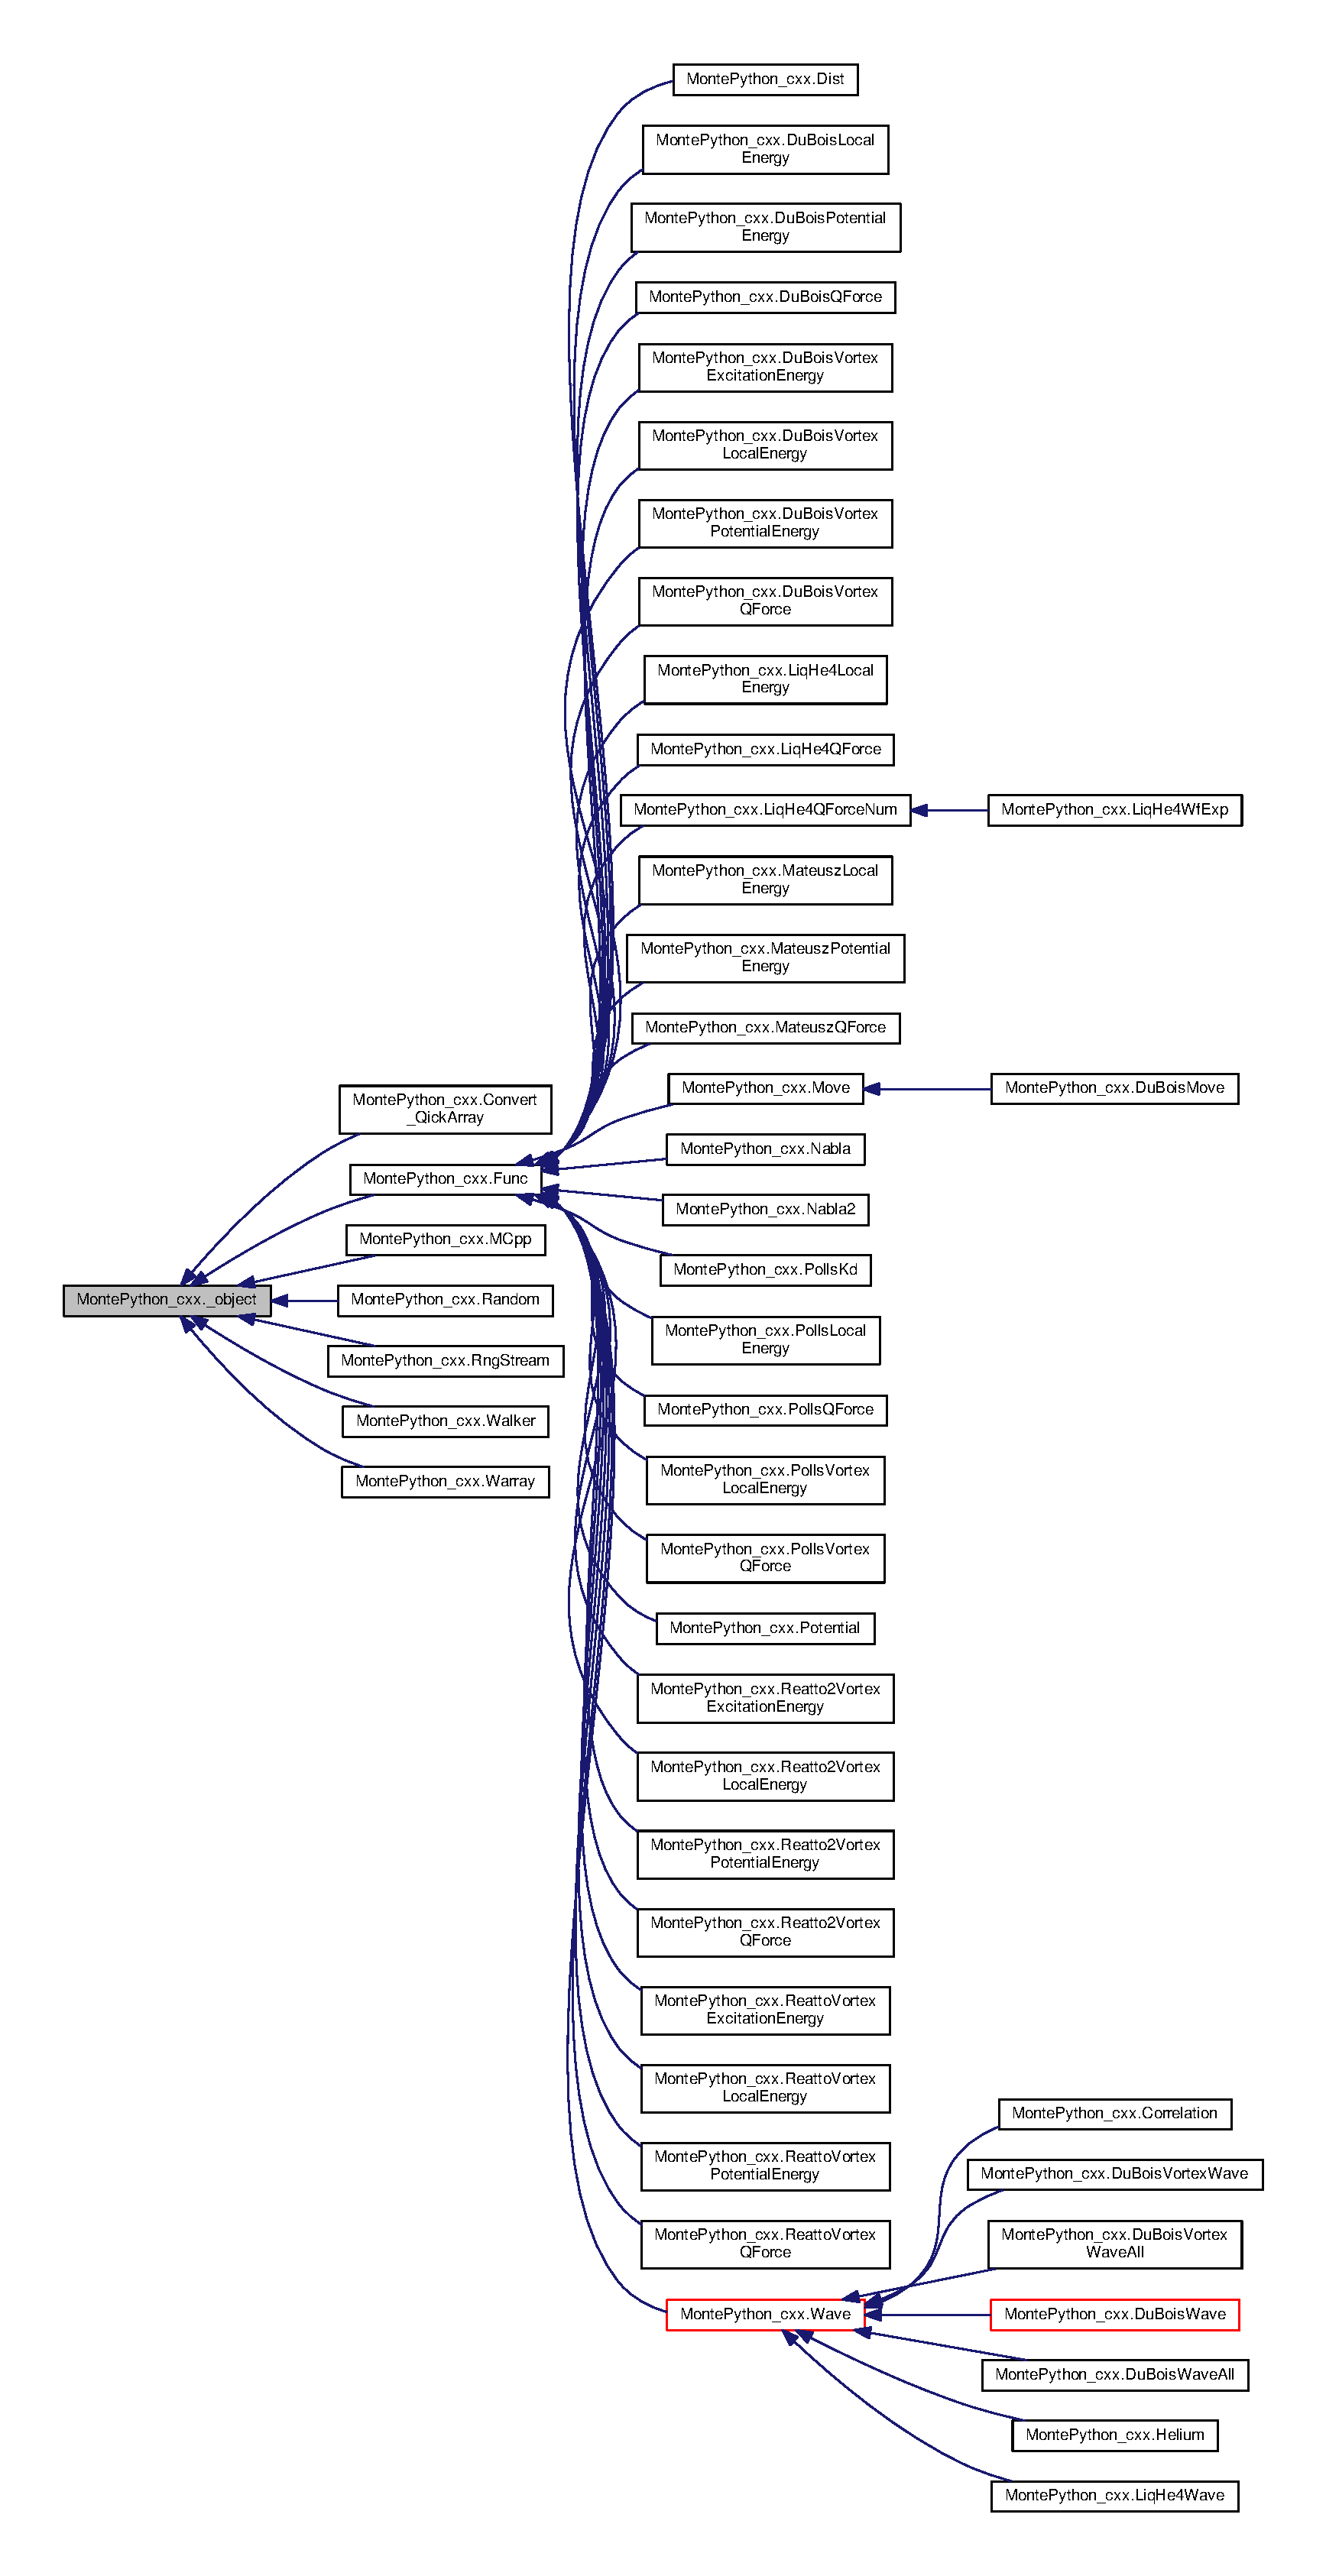
\includegraphics[height=550pt]{classMontePython__cxx_1_1__object__inherit__graph}
\end{center}
\end{figure}


The documentation for this class was generated from the following file\+:\begin{DoxyCompactItemize}
\item 
Monte\+Python\+\_\+cxx.\+py\end{DoxyCompactItemize}

\hypertarget{classMontePython__cxx_1_1Convert__QickArray}{}\section{Monte\+Python\+\_\+cxx.\+Convert\+\_\+\+Qick\+Array Class Reference}
\label{classMontePython__cxx_1_1Convert__QickArray}\index{Monte\+Python\+\_\+cxx.\+Convert\+\_\+\+Qick\+Array@{Monte\+Python\+\_\+cxx.\+Convert\+\_\+\+Qick\+Array}}


Inheritance diagram for Monte\+Python\+\_\+cxx.\+Convert\+\_\+\+Qick\+Array\+:
\nopagebreak
\begin{figure}[H]
\begin{center}
\leavevmode
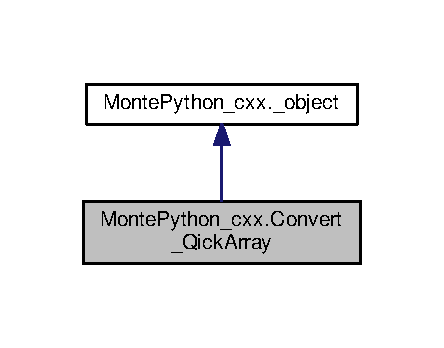
\includegraphics[width=213pt]{classMontePython__cxx_1_1Convert__QickArray__inherit__graph}
\end{center}
\end{figure}


Collaboration diagram for Monte\+Python\+\_\+cxx.\+Convert\+\_\+\+Qick\+Array\+:
\nopagebreak
\begin{figure}[H]
\begin{center}
\leavevmode
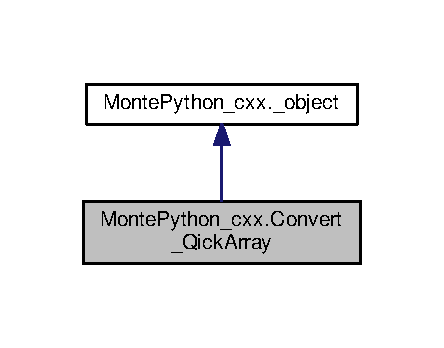
\includegraphics[width=213pt]{classMontePython__cxx_1_1Convert__QickArray__coll__graph}
\end{center}
\end{figure}
\subsection*{Public Member Functions}
\begin{DoxyCompactItemize}
\item 
def \hyperlink{classMontePython__cxx_1_1Convert__QickArray_a248fc9cad31385be9c478b1db0440e61}{\+\_\+\+\_\+init\+\_\+\+\_\+} (self)
\item 
def \hyperlink{classMontePython__cxx_1_1Convert__QickArray_a6042af47f1612c75887d899e3394988b}{my2py} (self, args)
\item 
def \hyperlink{classMontePython__cxx_1_1Convert__QickArray_a94d162d20ff1ada746f3449a7b84cb48}{py2my} (self, args)
\item 
def \hyperlink{classMontePython__cxx_1_1Convert__QickArray_aaf24ae72722f9469a90a6f7ef554ac4a}{my2py\+\_\+copy} (self, args)
\item 
def \hyperlink{classMontePython__cxx_1_1Convert__QickArray_a8c8bf46bde047728d8138ef632d31ad5}{py2my\+\_\+copy} (self, args)
\item 
def \hyperlink{classMontePython__cxx_1_1Convert__QickArray_a053da60df844cd2ff8b7264dd3416b7a}{dump} (self, args)
\end{DoxyCompactItemize}
\subsection*{Public Attributes}
\begin{DoxyCompactItemize}
\item 
\hypertarget{classMontePython__cxx_1_1Convert__QickArray_a8a2c164191969f58e9c2162b2a5f9a6f}{}{\bfseries this}\label{classMontePython__cxx_1_1Convert__QickArray_a8a2c164191969f58e9c2162b2a5f9a6f}

\end{DoxyCompactItemize}
\subsection*{Static Private Attributes}
\begin{DoxyCompactItemize}
\item 
\hypertarget{classMontePython__cxx_1_1Convert__QickArray_a362f999e51fc5045f9511471e5e1afc8}{}dictionary {\bfseries \+\_\+\+\_\+swig\+\_\+setmethods\+\_\+\+\_\+} = \{\}\label{classMontePython__cxx_1_1Convert__QickArray_a362f999e51fc5045f9511471e5e1afc8}

\item 
\hypertarget{classMontePython__cxx_1_1Convert__QickArray_a76d8184c750a0b62914cd166ff1f1754}{}tuple {\bfseries \+\_\+\+\_\+setattr\+\_\+\+\_\+} = lambdaself,name,value\+:\+\_\+swig\+\_\+setattr(self, \hyperlink{classMontePython__cxx_1_1Convert__QickArray}{Convert\+\_\+\+Qick\+Array}, name, value)\label{classMontePython__cxx_1_1Convert__QickArray_a76d8184c750a0b62914cd166ff1f1754}

\item 
\hypertarget{classMontePython__cxx_1_1Convert__QickArray_a57019f25e7bb80649b4b65e1613a0bc7}{}dictionary {\bfseries \+\_\+\+\_\+swig\+\_\+getmethods\+\_\+\+\_\+} = \{\}\label{classMontePython__cxx_1_1Convert__QickArray_a57019f25e7bb80649b4b65e1613a0bc7}

\item 
\hypertarget{classMontePython__cxx_1_1Convert__QickArray_ad1eab0b9364362ed6c36f1896e080993}{}tuple {\bfseries \+\_\+\+\_\+getattr\+\_\+\+\_\+} = lambdaself,name\+:\+\_\+swig\+\_\+getattr(self, \hyperlink{classMontePython__cxx_1_1Convert__QickArray}{Convert\+\_\+\+Qick\+Array}, name)\label{classMontePython__cxx_1_1Convert__QickArray_ad1eab0b9364362ed6c36f1896e080993}

\item 
\hypertarget{classMontePython__cxx_1_1Convert__QickArray_a10b77a508664a837fff2f88f65fea5b7}{}{\bfseries \+\_\+\+\_\+repr\+\_\+\+\_\+} = \+\_\+swig\+\_\+repr\label{classMontePython__cxx_1_1Convert__QickArray_a10b77a508664a837fff2f88f65fea5b7}

\item 
\hypertarget{classMontePython__cxx_1_1Convert__QickArray_a989ee4b28c717571eb3ddd100de9d9cc}{}{\bfseries \+\_\+\+\_\+swig\+\_\+destroy\+\_\+\+\_\+} = \+\_\+\+Monte\+Python\+\_\+cxx.\+delete\+\_\+\+Convert\+\_\+\+Qick\+Array\label{classMontePython__cxx_1_1Convert__QickArray_a989ee4b28c717571eb3ddd100de9d9cc}

\end{DoxyCompactItemize}


\subsection{Detailed Description}
\begin{DoxyVerb}Proxy of C++ Convert_QickArray class\end{DoxyVerb}
 

\subsection{Constructor \& Destructor Documentation}
\hypertarget{classMontePython__cxx_1_1Convert__QickArray_a248fc9cad31385be9c478b1db0440e61}{}\index{Monte\+Python\+\_\+cxx\+::\+Convert\+\_\+\+Qick\+Array@{Monte\+Python\+\_\+cxx\+::\+Convert\+\_\+\+Qick\+Array}!\+\_\+\+\_\+init\+\_\+\+\_\+@{\+\_\+\+\_\+init\+\_\+\+\_\+}}
\index{\+\_\+\+\_\+init\+\_\+\+\_\+@{\+\_\+\+\_\+init\+\_\+\+\_\+}!Monte\+Python\+\_\+cxx\+::\+Convert\+\_\+\+Qick\+Array@{Monte\+Python\+\_\+cxx\+::\+Convert\+\_\+\+Qick\+Array}}
\subsubsection[{\+\_\+\+\_\+init\+\_\+\+\_\+}]{\setlength{\rightskip}{0pt plus 5cm}def Monte\+Python\+\_\+cxx.\+Convert\+\_\+\+Qick\+Array.\+\_\+\+\_\+init\+\_\+\+\_\+ (
\begin{DoxyParamCaption}
\item[{}]{self}
\end{DoxyParamCaption}
)}\label{classMontePython__cxx_1_1Convert__QickArray_a248fc9cad31385be9c478b1db0440e61}
\begin{DoxyVerb}__init__(Convert_QickArray self) -> Convert_QickArray\end{DoxyVerb}
 

\subsection{Member Function Documentation}
\hypertarget{classMontePython__cxx_1_1Convert__QickArray_a053da60df844cd2ff8b7264dd3416b7a}{}\index{Monte\+Python\+\_\+cxx\+::\+Convert\+\_\+\+Qick\+Array@{Monte\+Python\+\_\+cxx\+::\+Convert\+\_\+\+Qick\+Array}!dump@{dump}}
\index{dump@{dump}!Monte\+Python\+\_\+cxx\+::\+Convert\+\_\+\+Qick\+Array@{Monte\+Python\+\_\+cxx\+::\+Convert\+\_\+\+Qick\+Array}}
\subsubsection[{dump}]{\setlength{\rightskip}{0pt plus 5cm}def Monte\+Python\+\_\+cxx.\+Convert\+\_\+\+Qick\+Array.\+dump (
\begin{DoxyParamCaption}
\item[{}]{self, }
\item[{}]{args}
\end{DoxyParamCaption}
)}\label{classMontePython__cxx_1_1Convert__QickArray_a053da60df844cd2ff8b7264dd3416b7a}
\begin{DoxyVerb}dump(Convert_QickArray self, QickArray & a)\end{DoxyVerb}
 \hypertarget{classMontePython__cxx_1_1Convert__QickArray_a6042af47f1612c75887d899e3394988b}{}\index{Monte\+Python\+\_\+cxx\+::\+Convert\+\_\+\+Qick\+Array@{Monte\+Python\+\_\+cxx\+::\+Convert\+\_\+\+Qick\+Array}!my2py@{my2py}}
\index{my2py@{my2py}!Monte\+Python\+\_\+cxx\+::\+Convert\+\_\+\+Qick\+Array@{Monte\+Python\+\_\+cxx\+::\+Convert\+\_\+\+Qick\+Array}}
\subsubsection[{my2py}]{\setlength{\rightskip}{0pt plus 5cm}def Monte\+Python\+\_\+cxx.\+Convert\+\_\+\+Qick\+Array.\+my2py (
\begin{DoxyParamCaption}
\item[{}]{self, }
\item[{}]{args}
\end{DoxyParamCaption}
)}\label{classMontePython__cxx_1_1Convert__QickArray_a6042af47f1612c75887d899e3394988b}
\begin{DoxyVerb}my2py(Convert_QickArray self, QickArray & a) -> PyObject *\end{DoxyVerb}
 \hypertarget{classMontePython__cxx_1_1Convert__QickArray_aaf24ae72722f9469a90a6f7ef554ac4a}{}\index{Monte\+Python\+\_\+cxx\+::\+Convert\+\_\+\+Qick\+Array@{Monte\+Python\+\_\+cxx\+::\+Convert\+\_\+\+Qick\+Array}!my2py\+\_\+copy@{my2py\+\_\+copy}}
\index{my2py\+\_\+copy@{my2py\+\_\+copy}!Monte\+Python\+\_\+cxx\+::\+Convert\+\_\+\+Qick\+Array@{Monte\+Python\+\_\+cxx\+::\+Convert\+\_\+\+Qick\+Array}}
\subsubsection[{my2py\+\_\+copy}]{\setlength{\rightskip}{0pt plus 5cm}def Monte\+Python\+\_\+cxx.\+Convert\+\_\+\+Qick\+Array.\+my2py\+\_\+copy (
\begin{DoxyParamCaption}
\item[{}]{self, }
\item[{}]{args}
\end{DoxyParamCaption}
)}\label{classMontePython__cxx_1_1Convert__QickArray_aaf24ae72722f9469a90a6f7ef554ac4a}
\begin{DoxyVerb}my2py_copy(Convert_QickArray self, QickArray & a) -> PyObject *\end{DoxyVerb}
 \hypertarget{classMontePython__cxx_1_1Convert__QickArray_a94d162d20ff1ada746f3449a7b84cb48}{}\index{Monte\+Python\+\_\+cxx\+::\+Convert\+\_\+\+Qick\+Array@{Monte\+Python\+\_\+cxx\+::\+Convert\+\_\+\+Qick\+Array}!py2my@{py2my}}
\index{py2my@{py2my}!Monte\+Python\+\_\+cxx\+::\+Convert\+\_\+\+Qick\+Array@{Monte\+Python\+\_\+cxx\+::\+Convert\+\_\+\+Qick\+Array}}
\subsubsection[{py2my}]{\setlength{\rightskip}{0pt plus 5cm}def Monte\+Python\+\_\+cxx.\+Convert\+\_\+\+Qick\+Array.\+py2my (
\begin{DoxyParamCaption}
\item[{}]{self, }
\item[{}]{args}
\end{DoxyParamCaption}
)}\label{classMontePython__cxx_1_1Convert__QickArray_a94d162d20ff1ada746f3449a7b84cb48}
\begin{DoxyVerb}py2my(Convert_QickArray self, PyObject * a) -> QickArray *\end{DoxyVerb}
 \hypertarget{classMontePython__cxx_1_1Convert__QickArray_a8c8bf46bde047728d8138ef632d31ad5}{}\index{Monte\+Python\+\_\+cxx\+::\+Convert\+\_\+\+Qick\+Array@{Monte\+Python\+\_\+cxx\+::\+Convert\+\_\+\+Qick\+Array}!py2my\+\_\+copy@{py2my\+\_\+copy}}
\index{py2my\+\_\+copy@{py2my\+\_\+copy}!Monte\+Python\+\_\+cxx\+::\+Convert\+\_\+\+Qick\+Array@{Monte\+Python\+\_\+cxx\+::\+Convert\+\_\+\+Qick\+Array}}
\subsubsection[{py2my\+\_\+copy}]{\setlength{\rightskip}{0pt plus 5cm}def Monte\+Python\+\_\+cxx.\+Convert\+\_\+\+Qick\+Array.\+py2my\+\_\+copy (
\begin{DoxyParamCaption}
\item[{}]{self, }
\item[{}]{args}
\end{DoxyParamCaption}
)}\label{classMontePython__cxx_1_1Convert__QickArray_a8c8bf46bde047728d8138ef632d31ad5}
\begin{DoxyVerb}py2my_copy(Convert_QickArray self, PyObject * a) -> QickArray *\end{DoxyVerb}
 

The documentation for this class was generated from the following file\+:\begin{DoxyCompactItemize}
\item 
Monte\+Python\+\_\+cxx.\+py\end{DoxyCompactItemize}

\hypertarget{classMontePython__cxx_1_1Correlation}{}\section{Monte\+Python\+\_\+cxx.\+Correlation Class Reference}
\label{classMontePython__cxx_1_1Correlation}\index{Monte\+Python\+\_\+cxx.\+Correlation@{Monte\+Python\+\_\+cxx.\+Correlation}}


Inheritance diagram for Monte\+Python\+\_\+cxx.\+Correlation\+:
\nopagebreak
\begin{figure}[H]
\begin{center}
\leavevmode
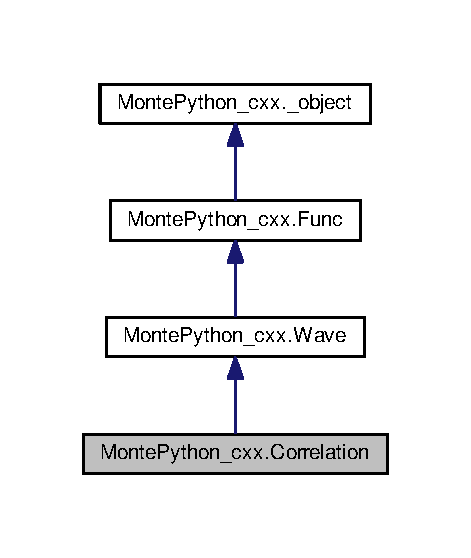
\includegraphics[width=226pt]{classMontePython__cxx_1_1Correlation__inherit__graph}
\end{center}
\end{figure}


Collaboration diagram for Monte\+Python\+\_\+cxx.\+Correlation\+:
\nopagebreak
\begin{figure}[H]
\begin{center}
\leavevmode
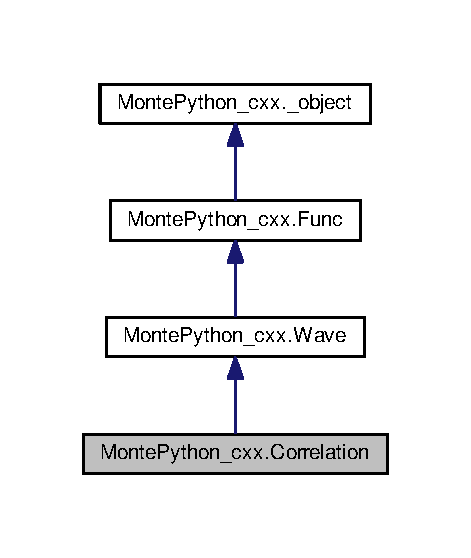
\includegraphics[width=226pt]{classMontePython__cxx_1_1Correlation__coll__graph}
\end{center}
\end{figure}
\subsection*{Public Member Functions}
\begin{DoxyCompactItemize}
\item 
def \hyperlink{classMontePython__cxx_1_1Correlation_abf182825b46e796e58dc7f1191c65495}{set\+Params} (self, args)
\item 
def \hyperlink{classMontePython__cxx_1_1Correlation_a8c0d313cd7e79d538349a59ce2afce09}{value\+Pt} (self, args)
\item 
def \hyperlink{classMontePython__cxx_1_1Correlation_a1f0c6fa3340d89d307623bd1c73fa65e}{\+\_\+\+\_\+call\+\_\+\+\_\+} (self, args)
\item 
def \hyperlink{classMontePython__cxx_1_1Correlation_a72322ab7109a1ba02acb2e17df7398fb}{\+\_\+\+\_\+init\+\_\+\+\_\+} (self)
\end{DoxyCompactItemize}
\subsection*{Public Attributes}
\begin{DoxyCompactItemize}
\item 
\hypertarget{classMontePython__cxx_1_1Correlation_a95ed7e076c2245aa470a3023149cc9b0}{}{\bfseries this}\label{classMontePython__cxx_1_1Correlation_a95ed7e076c2245aa470a3023149cc9b0}

\end{DoxyCompactItemize}
\subsection*{Static Private Attributes}
\begin{DoxyCompactItemize}
\item 
\hypertarget{classMontePython__cxx_1_1Correlation_ab7c6e3f139fa5e6ef7e4e256e8215009}{}dictionary {\bfseries \+\_\+\+\_\+swig\+\_\+setmethods\+\_\+\+\_\+} = \{\}\label{classMontePython__cxx_1_1Correlation_ab7c6e3f139fa5e6ef7e4e256e8215009}

\item 
\hypertarget{classMontePython__cxx_1_1Correlation_ace65695eb28b2191751afd09d203c377}{}tuple {\bfseries \+\_\+\+\_\+setattr\+\_\+\+\_\+} = lambdaself,name,value\+:\+\_\+swig\+\_\+setattr(self, \hyperlink{classMontePython__cxx_1_1Correlation}{Correlation}, name, value)\label{classMontePython__cxx_1_1Correlation_ace65695eb28b2191751afd09d203c377}

\item 
\hypertarget{classMontePython__cxx_1_1Correlation_a2c48587e7ea751d0f9ac3be2e8dc571b}{}dictionary {\bfseries \+\_\+\+\_\+swig\+\_\+getmethods\+\_\+\+\_\+} = \{\}\label{classMontePython__cxx_1_1Correlation_a2c48587e7ea751d0f9ac3be2e8dc571b}

\item 
\hypertarget{classMontePython__cxx_1_1Correlation_a4c4256508bce5a05cee26aad9971e6ea}{}tuple {\bfseries \+\_\+\+\_\+getattr\+\_\+\+\_\+} = lambdaself,name\+:\+\_\+swig\+\_\+getattr(self, \hyperlink{classMontePython__cxx_1_1Correlation}{Correlation}, name)\label{classMontePython__cxx_1_1Correlation_a4c4256508bce5a05cee26aad9971e6ea}

\item 
\hypertarget{classMontePython__cxx_1_1Correlation_a293c7ff649872a8aec72ce106086a7aa}{}{\bfseries \+\_\+\+\_\+repr\+\_\+\+\_\+} = \+\_\+swig\+\_\+repr\label{classMontePython__cxx_1_1Correlation_a293c7ff649872a8aec72ce106086a7aa}

\item 
\hypertarget{classMontePython__cxx_1_1Correlation_ae865672530d9d62b9017d712f720d1be}{}{\bfseries \+\_\+\+\_\+swig\+\_\+destroy\+\_\+\+\_\+} = \+\_\+\+Monte\+Python\+\_\+cxx.\+delete\+\_\+\+Correlation\label{classMontePython__cxx_1_1Correlation_ae865672530d9d62b9017d712f720d1be}

\end{DoxyCompactItemize}


\subsection{Detailed Description}
\begin{DoxyVerb}Proxy of C++ Correlation class\end{DoxyVerb}
 

\subsection{Constructor \& Destructor Documentation}
\hypertarget{classMontePython__cxx_1_1Correlation_a72322ab7109a1ba02acb2e17df7398fb}{}\index{Monte\+Python\+\_\+cxx\+::\+Correlation@{Monte\+Python\+\_\+cxx\+::\+Correlation}!\+\_\+\+\_\+init\+\_\+\+\_\+@{\+\_\+\+\_\+init\+\_\+\+\_\+}}
\index{\+\_\+\+\_\+init\+\_\+\+\_\+@{\+\_\+\+\_\+init\+\_\+\+\_\+}!Monte\+Python\+\_\+cxx\+::\+Correlation@{Monte\+Python\+\_\+cxx\+::\+Correlation}}
\subsubsection[{\+\_\+\+\_\+init\+\_\+\+\_\+}]{\setlength{\rightskip}{0pt plus 5cm}def Monte\+Python\+\_\+cxx.\+Correlation.\+\_\+\+\_\+init\+\_\+\+\_\+ (
\begin{DoxyParamCaption}
\item[{}]{self}
\end{DoxyParamCaption}
)}\label{classMontePython__cxx_1_1Correlation_a72322ab7109a1ba02acb2e17df7398fb}
\begin{DoxyVerb}__init__(Correlation self) -> Correlation\end{DoxyVerb}
 

\subsection{Member Function Documentation}
\hypertarget{classMontePython__cxx_1_1Correlation_a1f0c6fa3340d89d307623bd1c73fa65e}{}\index{Monte\+Python\+\_\+cxx\+::\+Correlation@{Monte\+Python\+\_\+cxx\+::\+Correlation}!\+\_\+\+\_\+call\+\_\+\+\_\+@{\+\_\+\+\_\+call\+\_\+\+\_\+}}
\index{\+\_\+\+\_\+call\+\_\+\+\_\+@{\+\_\+\+\_\+call\+\_\+\+\_\+}!Monte\+Python\+\_\+cxx\+::\+Correlation@{Monte\+Python\+\_\+cxx\+::\+Correlation}}
\subsubsection[{\+\_\+\+\_\+call\+\_\+\+\_\+}]{\setlength{\rightskip}{0pt plus 5cm}def Monte\+Python\+\_\+cxx.\+Correlation.\+\_\+\+\_\+call\+\_\+\+\_\+ (
\begin{DoxyParamCaption}
\item[{}]{self, }
\item[{}]{args}
\end{DoxyParamCaption}
)}\label{classMontePython__cxx_1_1Correlation_a1f0c6fa3340d89d307623bd1c73fa65e}
\begin{DoxyVerb}__call__(Correlation self, QickArray & pos) -> double\end{DoxyVerb}
 \hypertarget{classMontePython__cxx_1_1Correlation_abf182825b46e796e58dc7f1191c65495}{}\index{Monte\+Python\+\_\+cxx\+::\+Correlation@{Monte\+Python\+\_\+cxx\+::\+Correlation}!set\+Params@{set\+Params}}
\index{set\+Params@{set\+Params}!Monte\+Python\+\_\+cxx\+::\+Correlation@{Monte\+Python\+\_\+cxx\+::\+Correlation}}
\subsubsection[{set\+Params}]{\setlength{\rightskip}{0pt plus 5cm}def Monte\+Python\+\_\+cxx.\+Correlation.\+set\+Params (
\begin{DoxyParamCaption}
\item[{}]{self, }
\item[{}]{args}
\end{DoxyParamCaption}
)}\label{classMontePython__cxx_1_1Correlation_abf182825b46e796e58dc7f1191c65495}
\begin{DoxyVerb}setParams(Correlation self, QickArray & params_)\end{DoxyVerb}
 \hypertarget{classMontePython__cxx_1_1Correlation_a8c0d313cd7e79d538349a59ce2afce09}{}\index{Monte\+Python\+\_\+cxx\+::\+Correlation@{Monte\+Python\+\_\+cxx\+::\+Correlation}!value\+Pt@{value\+Pt}}
\index{value\+Pt@{value\+Pt}!Monte\+Python\+\_\+cxx\+::\+Correlation@{Monte\+Python\+\_\+cxx\+::\+Correlation}}
\subsubsection[{value\+Pt}]{\setlength{\rightskip}{0pt plus 5cm}def Monte\+Python\+\_\+cxx.\+Correlation.\+value\+Pt (
\begin{DoxyParamCaption}
\item[{}]{self, }
\item[{}]{args}
\end{DoxyParamCaption}
)}\label{classMontePython__cxx_1_1Correlation_a8c0d313cd7e79d538349a59ce2afce09}
\begin{DoxyVerb}valuePt(Correlation self, QickArray & pos) -> double\end{DoxyVerb}
 

The documentation for this class was generated from the following file\+:\begin{DoxyCompactItemize}
\item 
Monte\+Python\+\_\+cxx.\+py\end{DoxyCompactItemize}

\hypertarget{classMontePython__cxx_1_1Dist}{}\section{Monte\+Python\+\_\+cxx.\+Dist Class Reference}
\label{classMontePython__cxx_1_1Dist}\index{Monte\+Python\+\_\+cxx.\+Dist@{Monte\+Python\+\_\+cxx.\+Dist}}


Inheritance diagram for Monte\+Python\+\_\+cxx.\+Dist\+:
\nopagebreak
\begin{figure}[H]
\begin{center}
\leavevmode
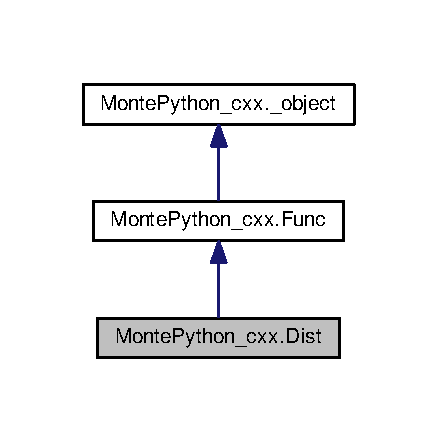
\includegraphics[width=210pt]{classMontePython__cxx_1_1Dist__inherit__graph}
\end{center}
\end{figure}


Collaboration diagram for Monte\+Python\+\_\+cxx.\+Dist\+:
\nopagebreak
\begin{figure}[H]
\begin{center}
\leavevmode
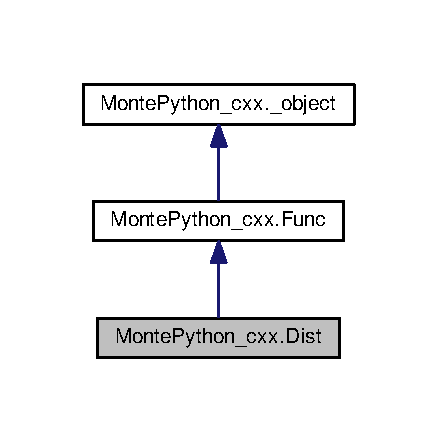
\includegraphics[width=210pt]{classMontePython__cxx_1_1Dist__coll__graph}
\end{center}
\end{figure}
\subsection*{Public Member Functions}
\begin{DoxyCompactItemize}
\item 
def \hyperlink{classMontePython__cxx_1_1Dist_a476c97823f5262aef7efb979be8cceb8}{value\+Pt} (self, args)
\item 
def \hyperlink{classMontePython__cxx_1_1Dist_a2a00e84f2fc6061f0b1c8c01265c5e1b}{\+\_\+\+\_\+call\+\_\+\+\_\+} (self, args)
\item 
def \hyperlink{classMontePython__cxx_1_1Dist_ac13e88a03dec3a6613c077d4e940b9f5}{\+\_\+\+\_\+init\+\_\+\+\_\+} (self)
\end{DoxyCompactItemize}
\subsection*{Public Attributes}
\begin{DoxyCompactItemize}
\item 
\hypertarget{classMontePython__cxx_1_1Dist_a9236d8349ac58fced7859c6b546ebc00}{}{\bfseries this}\label{classMontePython__cxx_1_1Dist_a9236d8349ac58fced7859c6b546ebc00}

\end{DoxyCompactItemize}
\subsection*{Static Private Attributes}
\begin{DoxyCompactItemize}
\item 
\hypertarget{classMontePython__cxx_1_1Dist_acd9b935c74e8df2e3380b8f72cc3c19f}{}dictionary {\bfseries \+\_\+\+\_\+swig\+\_\+setmethods\+\_\+\+\_\+} = \{\}\label{classMontePython__cxx_1_1Dist_acd9b935c74e8df2e3380b8f72cc3c19f}

\item 
\hypertarget{classMontePython__cxx_1_1Dist_a12aa3c9146a49d6708e5c58215090139}{}tuple {\bfseries \+\_\+\+\_\+setattr\+\_\+\+\_\+} = lambdaself,name,value\+:\+\_\+swig\+\_\+setattr(self, \hyperlink{classMontePython__cxx_1_1Dist}{Dist}, name, value)\label{classMontePython__cxx_1_1Dist_a12aa3c9146a49d6708e5c58215090139}

\item 
\hypertarget{classMontePython__cxx_1_1Dist_a95e97f322b4bf5a748f0e92cbc771665}{}dictionary {\bfseries \+\_\+\+\_\+swig\+\_\+getmethods\+\_\+\+\_\+} = \{\}\label{classMontePython__cxx_1_1Dist_a95e97f322b4bf5a748f0e92cbc771665}

\item 
\hypertarget{classMontePython__cxx_1_1Dist_a4a1697eb64141a1bd636b41b27fdb17b}{}tuple {\bfseries \+\_\+\+\_\+getattr\+\_\+\+\_\+} = lambdaself,name\+:\+\_\+swig\+\_\+getattr(self, \hyperlink{classMontePython__cxx_1_1Dist}{Dist}, name)\label{classMontePython__cxx_1_1Dist_a4a1697eb64141a1bd636b41b27fdb17b}

\item 
\hypertarget{classMontePython__cxx_1_1Dist_a26520ef017a9f08c26a5c4cfde0b0217}{}{\bfseries \+\_\+\+\_\+repr\+\_\+\+\_\+} = \+\_\+swig\+\_\+repr\label{classMontePython__cxx_1_1Dist_a26520ef017a9f08c26a5c4cfde0b0217}

\item 
\hypertarget{classMontePython__cxx_1_1Dist_a61e6995208c0ffc17d1bb646b031e827}{}{\bfseries \+\_\+\+\_\+swig\+\_\+destroy\+\_\+\+\_\+} = \+\_\+\+Monte\+Python\+\_\+cxx.\+delete\+\_\+\+Dist\label{classMontePython__cxx_1_1Dist_a61e6995208c0ffc17d1bb646b031e827}

\end{DoxyCompactItemize}


\subsection{Detailed Description}
\begin{DoxyVerb}Proxy of C++ Dist class\end{DoxyVerb}
 

\subsection{Constructor \& Destructor Documentation}
\hypertarget{classMontePython__cxx_1_1Dist_ac13e88a03dec3a6613c077d4e940b9f5}{}\index{Monte\+Python\+\_\+cxx\+::\+Dist@{Monte\+Python\+\_\+cxx\+::\+Dist}!\+\_\+\+\_\+init\+\_\+\+\_\+@{\+\_\+\+\_\+init\+\_\+\+\_\+}}
\index{\+\_\+\+\_\+init\+\_\+\+\_\+@{\+\_\+\+\_\+init\+\_\+\+\_\+}!Monte\+Python\+\_\+cxx\+::\+Dist@{Monte\+Python\+\_\+cxx\+::\+Dist}}
\subsubsection[{\+\_\+\+\_\+init\+\_\+\+\_\+}]{\setlength{\rightskip}{0pt plus 5cm}def Monte\+Python\+\_\+cxx.\+Dist.\+\_\+\+\_\+init\+\_\+\+\_\+ (
\begin{DoxyParamCaption}
\item[{}]{self}
\end{DoxyParamCaption}
)}\label{classMontePython__cxx_1_1Dist_ac13e88a03dec3a6613c077d4e940b9f5}
\begin{DoxyVerb}__init__(Dist self) -> Dist\end{DoxyVerb}
 

\subsection{Member Function Documentation}
\hypertarget{classMontePython__cxx_1_1Dist_a2a00e84f2fc6061f0b1c8c01265c5e1b}{}\index{Monte\+Python\+\_\+cxx\+::\+Dist@{Monte\+Python\+\_\+cxx\+::\+Dist}!\+\_\+\+\_\+call\+\_\+\+\_\+@{\+\_\+\+\_\+call\+\_\+\+\_\+}}
\index{\+\_\+\+\_\+call\+\_\+\+\_\+@{\+\_\+\+\_\+call\+\_\+\+\_\+}!Monte\+Python\+\_\+cxx\+::\+Dist@{Monte\+Python\+\_\+cxx\+::\+Dist}}
\subsubsection[{\+\_\+\+\_\+call\+\_\+\+\_\+}]{\setlength{\rightskip}{0pt plus 5cm}def Monte\+Python\+\_\+cxx.\+Dist.\+\_\+\+\_\+call\+\_\+\+\_\+ (
\begin{DoxyParamCaption}
\item[{}]{self, }
\item[{}]{args}
\end{DoxyParamCaption}
)}\label{classMontePython__cxx_1_1Dist_a2a00e84f2fc6061f0b1c8c01265c5e1b}
\begin{DoxyVerb}__call__(Dist self, QickArray & pos, double l) -> QickArray &\end{DoxyVerb}
 \hypertarget{classMontePython__cxx_1_1Dist_a476c97823f5262aef7efb979be8cceb8}{}\index{Monte\+Python\+\_\+cxx\+::\+Dist@{Monte\+Python\+\_\+cxx\+::\+Dist}!value\+Pt@{value\+Pt}}
\index{value\+Pt@{value\+Pt}!Monte\+Python\+\_\+cxx\+::\+Dist@{Monte\+Python\+\_\+cxx\+::\+Dist}}
\subsubsection[{value\+Pt}]{\setlength{\rightskip}{0pt plus 5cm}def Monte\+Python\+\_\+cxx.\+Dist.\+value\+Pt (
\begin{DoxyParamCaption}
\item[{}]{self, }
\item[{}]{args}
\end{DoxyParamCaption}
)}\label{classMontePython__cxx_1_1Dist_a476c97823f5262aef7efb979be8cceb8}
\begin{DoxyVerb}valuePt(Dist self, QickArray & pos, double l) -> QickArray &\end{DoxyVerb}
 

The documentation for this class was generated from the following file\+:\begin{DoxyCompactItemize}
\item 
Monte\+Python\+\_\+cxx.\+py\end{DoxyCompactItemize}

\hypertarget{classMontePython__cxx_1_1DuBoisGauss}{}\section{Monte\+Python\+\_\+cxx.\+Du\+Bois\+Gauss Class Reference}
\label{classMontePython__cxx_1_1DuBoisGauss}\index{Monte\+Python\+\_\+cxx.\+Du\+Bois\+Gauss@{Monte\+Python\+\_\+cxx.\+Du\+Bois\+Gauss}}


Inheritance diagram for Monte\+Python\+\_\+cxx.\+Du\+Bois\+Gauss\+:
\nopagebreak
\begin{figure}[H]
\begin{center}
\leavevmode
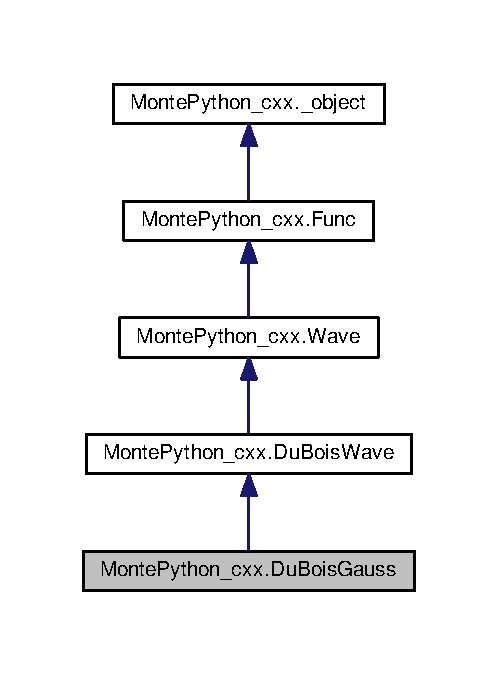
\includegraphics[width=239pt]{classMontePython__cxx_1_1DuBoisGauss__inherit__graph}
\end{center}
\end{figure}


Collaboration diagram for Monte\+Python\+\_\+cxx.\+Du\+Bois\+Gauss\+:
\nopagebreak
\begin{figure}[H]
\begin{center}
\leavevmode
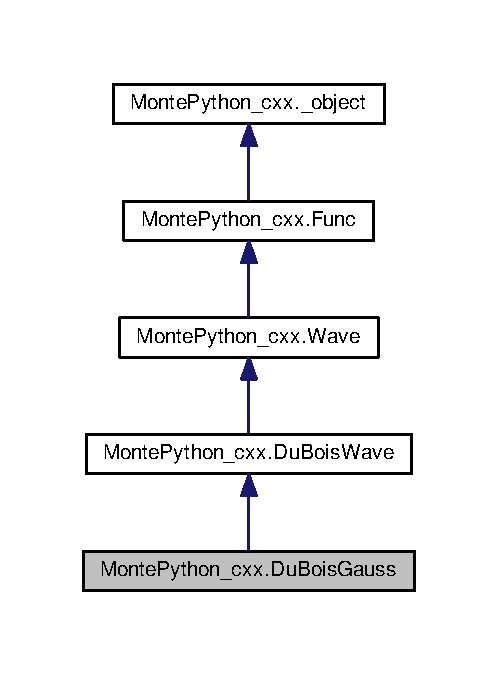
\includegraphics[width=239pt]{classMontePython__cxx_1_1DuBoisGauss__coll__graph}
\end{center}
\end{figure}
\subsection*{Public Member Functions}
\begin{DoxyCompactItemize}
\item 
def \hyperlink{classMontePython__cxx_1_1DuBoisGauss_a787908576ab3659adabe93ea9a8a6639}{value\+Pt} (self, args)
\item 
def \hyperlink{classMontePython__cxx_1_1DuBoisGauss_a38fa91aca193bcccde433013a04f9125}{\+\_\+\+\_\+call\+\_\+\+\_\+} (self, args)
\item 
def \hyperlink{classMontePython__cxx_1_1DuBoisGauss_a5dec80e93e531f4cacec418699cfbf16}{\+\_\+\+\_\+init\+\_\+\+\_\+} (self)
\end{DoxyCompactItemize}
\subsection*{Public Attributes}
\begin{DoxyCompactItemize}
\item 
\hypertarget{classMontePython__cxx_1_1DuBoisGauss_a680a7dc0120737a77f4ccea839b575c7}{}{\bfseries this}\label{classMontePython__cxx_1_1DuBoisGauss_a680a7dc0120737a77f4ccea839b575c7}

\end{DoxyCompactItemize}
\subsection*{Static Private Attributes}
\begin{DoxyCompactItemize}
\item 
\hypertarget{classMontePython__cxx_1_1DuBoisGauss_a433eaf202c7a171fb7498e6e7e54da9a}{}dictionary {\bfseries \+\_\+\+\_\+swig\+\_\+setmethods\+\_\+\+\_\+} = \{\}\label{classMontePython__cxx_1_1DuBoisGauss_a433eaf202c7a171fb7498e6e7e54da9a}

\item 
\hypertarget{classMontePython__cxx_1_1DuBoisGauss_a89306da6dc501c11a27108b24e1edf35}{}tuple {\bfseries \+\_\+\+\_\+setattr\+\_\+\+\_\+} = lambdaself,name,value\+:\+\_\+swig\+\_\+setattr(self, \hyperlink{classMontePython__cxx_1_1DuBoisGauss}{Du\+Bois\+Gauss}, name, value)\label{classMontePython__cxx_1_1DuBoisGauss_a89306da6dc501c11a27108b24e1edf35}

\item 
\hypertarget{classMontePython__cxx_1_1DuBoisGauss_ad886a66d3ab5c237fe5ac7d55e07e958}{}dictionary {\bfseries \+\_\+\+\_\+swig\+\_\+getmethods\+\_\+\+\_\+} = \{\}\label{classMontePython__cxx_1_1DuBoisGauss_ad886a66d3ab5c237fe5ac7d55e07e958}

\item 
\hypertarget{classMontePython__cxx_1_1DuBoisGauss_aa8ae51d7234ced5c0ec8c2ac099fd9fc}{}tuple {\bfseries \+\_\+\+\_\+getattr\+\_\+\+\_\+} = lambdaself,name\+:\+\_\+swig\+\_\+getattr(self, \hyperlink{classMontePython__cxx_1_1DuBoisGauss}{Du\+Bois\+Gauss}, name)\label{classMontePython__cxx_1_1DuBoisGauss_aa8ae51d7234ced5c0ec8c2ac099fd9fc}

\item 
\hypertarget{classMontePython__cxx_1_1DuBoisGauss_afd54d91061c53cbc7e226c2a263affea}{}{\bfseries \+\_\+\+\_\+repr\+\_\+\+\_\+} = \+\_\+swig\+\_\+repr\label{classMontePython__cxx_1_1DuBoisGauss_afd54d91061c53cbc7e226c2a263affea}

\item 
\hypertarget{classMontePython__cxx_1_1DuBoisGauss_acbf285cdd4ad5fb5e1b578e9f1328d20}{}{\bfseries \+\_\+\+\_\+swig\+\_\+destroy\+\_\+\+\_\+} = \+\_\+\+Monte\+Python\+\_\+cxx.\+delete\+\_\+\+Du\+Bois\+Gauss\label{classMontePython__cxx_1_1DuBoisGauss_acbf285cdd4ad5fb5e1b578e9f1328d20}

\end{DoxyCompactItemize}


\subsection{Detailed Description}
\begin{DoxyVerb}Proxy of C++ DuBoisGauss class\end{DoxyVerb}
 

\subsection{Constructor \& Destructor Documentation}
\hypertarget{classMontePython__cxx_1_1DuBoisGauss_a5dec80e93e531f4cacec418699cfbf16}{}\index{Monte\+Python\+\_\+cxx\+::\+Du\+Bois\+Gauss@{Monte\+Python\+\_\+cxx\+::\+Du\+Bois\+Gauss}!\+\_\+\+\_\+init\+\_\+\+\_\+@{\+\_\+\+\_\+init\+\_\+\+\_\+}}
\index{\+\_\+\+\_\+init\+\_\+\+\_\+@{\+\_\+\+\_\+init\+\_\+\+\_\+}!Monte\+Python\+\_\+cxx\+::\+Du\+Bois\+Gauss@{Monte\+Python\+\_\+cxx\+::\+Du\+Bois\+Gauss}}
\subsubsection[{\+\_\+\+\_\+init\+\_\+\+\_\+}]{\setlength{\rightskip}{0pt plus 5cm}def Monte\+Python\+\_\+cxx.\+Du\+Bois\+Gauss.\+\_\+\+\_\+init\+\_\+\+\_\+ (
\begin{DoxyParamCaption}
\item[{}]{self}
\end{DoxyParamCaption}
)}\label{classMontePython__cxx_1_1DuBoisGauss_a5dec80e93e531f4cacec418699cfbf16}
\begin{DoxyVerb}__init__(DuBoisGauss self) -> DuBoisGauss\end{DoxyVerb}
 

\subsection{Member Function Documentation}
\hypertarget{classMontePython__cxx_1_1DuBoisGauss_a38fa91aca193bcccde433013a04f9125}{}\index{Monte\+Python\+\_\+cxx\+::\+Du\+Bois\+Gauss@{Monte\+Python\+\_\+cxx\+::\+Du\+Bois\+Gauss}!\+\_\+\+\_\+call\+\_\+\+\_\+@{\+\_\+\+\_\+call\+\_\+\+\_\+}}
\index{\+\_\+\+\_\+call\+\_\+\+\_\+@{\+\_\+\+\_\+call\+\_\+\+\_\+}!Monte\+Python\+\_\+cxx\+::\+Du\+Bois\+Gauss@{Monte\+Python\+\_\+cxx\+::\+Du\+Bois\+Gauss}}
\subsubsection[{\+\_\+\+\_\+call\+\_\+\+\_\+}]{\setlength{\rightskip}{0pt plus 5cm}def Monte\+Python\+\_\+cxx.\+Du\+Bois\+Gauss.\+\_\+\+\_\+call\+\_\+\+\_\+ (
\begin{DoxyParamCaption}
\item[{}]{self, }
\item[{}]{args}
\end{DoxyParamCaption}
)}\label{classMontePython__cxx_1_1DuBoisGauss_a38fa91aca193bcccde433013a04f9125}
\begin{DoxyVerb}__call__(DuBoisGauss self, QickArray & pos) -> double\end{DoxyVerb}
 \hypertarget{classMontePython__cxx_1_1DuBoisGauss_a787908576ab3659adabe93ea9a8a6639}{}\index{Monte\+Python\+\_\+cxx\+::\+Du\+Bois\+Gauss@{Monte\+Python\+\_\+cxx\+::\+Du\+Bois\+Gauss}!value\+Pt@{value\+Pt}}
\index{value\+Pt@{value\+Pt}!Monte\+Python\+\_\+cxx\+::\+Du\+Bois\+Gauss@{Monte\+Python\+\_\+cxx\+::\+Du\+Bois\+Gauss}}
\subsubsection[{value\+Pt}]{\setlength{\rightskip}{0pt plus 5cm}def Monte\+Python\+\_\+cxx.\+Du\+Bois\+Gauss.\+value\+Pt (
\begin{DoxyParamCaption}
\item[{}]{self, }
\item[{}]{args}
\end{DoxyParamCaption}
)}\label{classMontePython__cxx_1_1DuBoisGauss_a787908576ab3659adabe93ea9a8a6639}
\begin{DoxyVerb}valuePt(DuBoisGauss self, QickArray & pos) -> double\end{DoxyVerb}
 

The documentation for this class was generated from the following file\+:\begin{DoxyCompactItemize}
\item 
Monte\+Python\+\_\+cxx.\+py\end{DoxyCompactItemize}

\hypertarget{classMontePython__cxx_1_1DuBoisJastrow}{}\section{Monte\+Python\+\_\+cxx.\+Du\+Bois\+Jastrow Class Reference}
\label{classMontePython__cxx_1_1DuBoisJastrow}\index{Monte\+Python\+\_\+cxx.\+Du\+Bois\+Jastrow@{Monte\+Python\+\_\+cxx.\+Du\+Bois\+Jastrow}}


Inheritance diagram for Monte\+Python\+\_\+cxx.\+Du\+Bois\+Jastrow\+:
\nopagebreak
\begin{figure}[H]
\begin{center}
\leavevmode
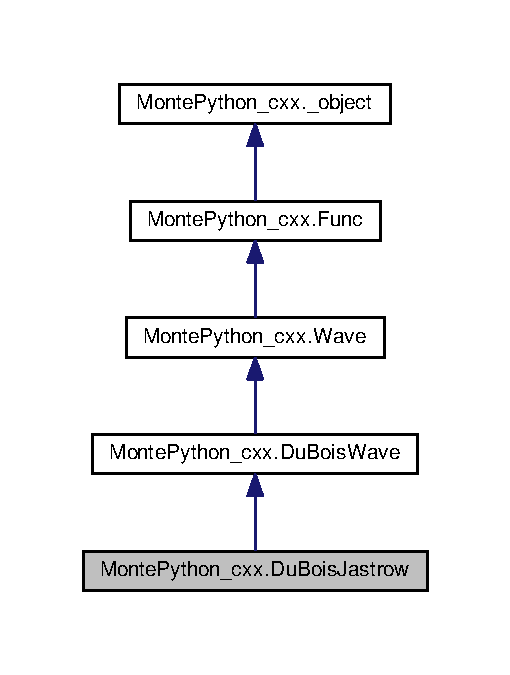
\includegraphics[width=245pt]{classMontePython__cxx_1_1DuBoisJastrow__inherit__graph}
\end{center}
\end{figure}


Collaboration diagram for Monte\+Python\+\_\+cxx.\+Du\+Bois\+Jastrow\+:
\nopagebreak
\begin{figure}[H]
\begin{center}
\leavevmode
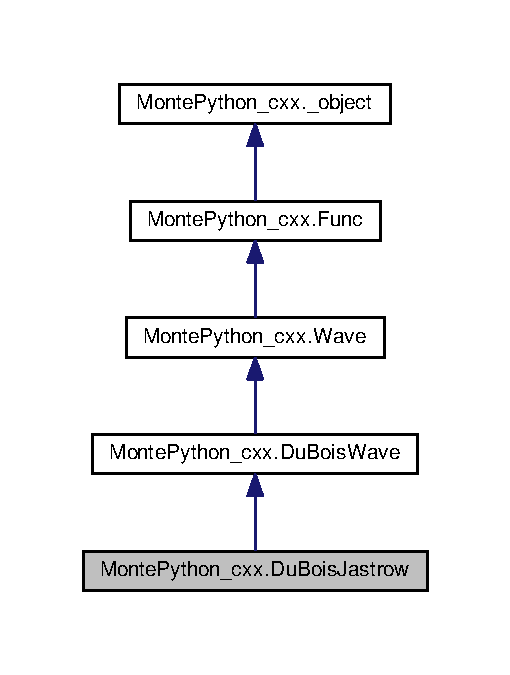
\includegraphics[width=245pt]{classMontePython__cxx_1_1DuBoisJastrow__coll__graph}
\end{center}
\end{figure}
\subsection*{Public Member Functions}
\begin{DoxyCompactItemize}
\item 
def \hyperlink{classMontePython__cxx_1_1DuBoisJastrow_a659649ff4b7e94df0de61f02000ca145}{set\+Params} (self, args)
\item 
def \hyperlink{classMontePython__cxx_1_1DuBoisJastrow_ab11797d6cc1f39dfe435a00813c84e2d}{value\+Pt} (self, args)
\item 
def \hyperlink{classMontePython__cxx_1_1DuBoisJastrow_a8427ec3cef4cf56875c3b905be82591c}{\+\_\+\+\_\+call\+\_\+\+\_\+} (self, args)
\item 
def \hyperlink{classMontePython__cxx_1_1DuBoisJastrow_ad3066d0cb1c1fb05b7981208b0bb2f61}{\+\_\+\+\_\+init\+\_\+\+\_\+} (self)
\end{DoxyCompactItemize}
\subsection*{Public Attributes}
\begin{DoxyCompactItemize}
\item 
\hypertarget{classMontePython__cxx_1_1DuBoisJastrow_a36f6bc926cef38dbfd68d9255dd5fbf4}{}{\bfseries this}\label{classMontePython__cxx_1_1DuBoisJastrow_a36f6bc926cef38dbfd68d9255dd5fbf4}

\end{DoxyCompactItemize}
\subsection*{Static Private Attributes}
\begin{DoxyCompactItemize}
\item 
\hypertarget{classMontePython__cxx_1_1DuBoisJastrow_a732f9b837b386085402f1f03011d7539}{}dictionary {\bfseries \+\_\+\+\_\+swig\+\_\+setmethods\+\_\+\+\_\+} = \{\}\label{classMontePython__cxx_1_1DuBoisJastrow_a732f9b837b386085402f1f03011d7539}

\item 
\hypertarget{classMontePython__cxx_1_1DuBoisJastrow_acb3d90c5bdc55fd408e559f2d5fac170}{}tuple {\bfseries \+\_\+\+\_\+setattr\+\_\+\+\_\+} = lambdaself,name,value\+:\+\_\+swig\+\_\+setattr(self, \hyperlink{classMontePython__cxx_1_1DuBoisJastrow}{Du\+Bois\+Jastrow}, name, value)\label{classMontePython__cxx_1_1DuBoisJastrow_acb3d90c5bdc55fd408e559f2d5fac170}

\item 
\hypertarget{classMontePython__cxx_1_1DuBoisJastrow_a7ad1853b1e6bea21055c01d6d36e38ff}{}dictionary {\bfseries \+\_\+\+\_\+swig\+\_\+getmethods\+\_\+\+\_\+} = \{\}\label{classMontePython__cxx_1_1DuBoisJastrow_a7ad1853b1e6bea21055c01d6d36e38ff}

\item 
\hypertarget{classMontePython__cxx_1_1DuBoisJastrow_af15ca982a357ec9f2b730cc644890070}{}tuple {\bfseries \+\_\+\+\_\+getattr\+\_\+\+\_\+} = lambdaself,name\+:\+\_\+swig\+\_\+getattr(self, \hyperlink{classMontePython__cxx_1_1DuBoisJastrow}{Du\+Bois\+Jastrow}, name)\label{classMontePython__cxx_1_1DuBoisJastrow_af15ca982a357ec9f2b730cc644890070}

\item 
\hypertarget{classMontePython__cxx_1_1DuBoisJastrow_aee807c361d3b6f7b436b1275c24107de}{}{\bfseries \+\_\+\+\_\+repr\+\_\+\+\_\+} = \+\_\+swig\+\_\+repr\label{classMontePython__cxx_1_1DuBoisJastrow_aee807c361d3b6f7b436b1275c24107de}

\item 
\hypertarget{classMontePython__cxx_1_1DuBoisJastrow_a77a3629416a5c2894fdd68b7d18d9dab}{}{\bfseries \+\_\+\+\_\+swig\+\_\+destroy\+\_\+\+\_\+} = \+\_\+\+Monte\+Python\+\_\+cxx.\+delete\+\_\+\+Du\+Bois\+Jastrow\label{classMontePython__cxx_1_1DuBoisJastrow_a77a3629416a5c2894fdd68b7d18d9dab}

\end{DoxyCompactItemize}


\subsection{Detailed Description}
\begin{DoxyVerb}Proxy of C++ DuBoisJastrow class\end{DoxyVerb}
 

\subsection{Constructor \& Destructor Documentation}
\hypertarget{classMontePython__cxx_1_1DuBoisJastrow_ad3066d0cb1c1fb05b7981208b0bb2f61}{}\index{Monte\+Python\+\_\+cxx\+::\+Du\+Bois\+Jastrow@{Monte\+Python\+\_\+cxx\+::\+Du\+Bois\+Jastrow}!\+\_\+\+\_\+init\+\_\+\+\_\+@{\+\_\+\+\_\+init\+\_\+\+\_\+}}
\index{\+\_\+\+\_\+init\+\_\+\+\_\+@{\+\_\+\+\_\+init\+\_\+\+\_\+}!Monte\+Python\+\_\+cxx\+::\+Du\+Bois\+Jastrow@{Monte\+Python\+\_\+cxx\+::\+Du\+Bois\+Jastrow}}
\subsubsection[{\+\_\+\+\_\+init\+\_\+\+\_\+}]{\setlength{\rightskip}{0pt plus 5cm}def Monte\+Python\+\_\+cxx.\+Du\+Bois\+Jastrow.\+\_\+\+\_\+init\+\_\+\+\_\+ (
\begin{DoxyParamCaption}
\item[{}]{self}
\end{DoxyParamCaption}
)}\label{classMontePython__cxx_1_1DuBoisJastrow_ad3066d0cb1c1fb05b7981208b0bb2f61}
\begin{DoxyVerb}__init__(DuBoisJastrow self) -> DuBoisJastrow\end{DoxyVerb}
 

\subsection{Member Function Documentation}
\hypertarget{classMontePython__cxx_1_1DuBoisJastrow_a8427ec3cef4cf56875c3b905be82591c}{}\index{Monte\+Python\+\_\+cxx\+::\+Du\+Bois\+Jastrow@{Monte\+Python\+\_\+cxx\+::\+Du\+Bois\+Jastrow}!\+\_\+\+\_\+call\+\_\+\+\_\+@{\+\_\+\+\_\+call\+\_\+\+\_\+}}
\index{\+\_\+\+\_\+call\+\_\+\+\_\+@{\+\_\+\+\_\+call\+\_\+\+\_\+}!Monte\+Python\+\_\+cxx\+::\+Du\+Bois\+Jastrow@{Monte\+Python\+\_\+cxx\+::\+Du\+Bois\+Jastrow}}
\subsubsection[{\+\_\+\+\_\+call\+\_\+\+\_\+}]{\setlength{\rightskip}{0pt plus 5cm}def Monte\+Python\+\_\+cxx.\+Du\+Bois\+Jastrow.\+\_\+\+\_\+call\+\_\+\+\_\+ (
\begin{DoxyParamCaption}
\item[{}]{self, }
\item[{}]{args}
\end{DoxyParamCaption}
)}\label{classMontePython__cxx_1_1DuBoisJastrow_a8427ec3cef4cf56875c3b905be82591c}
\begin{DoxyVerb}__call__(DuBoisJastrow self, QickArray & pos) -> double\end{DoxyVerb}
 \hypertarget{classMontePython__cxx_1_1DuBoisJastrow_a659649ff4b7e94df0de61f02000ca145}{}\index{Monte\+Python\+\_\+cxx\+::\+Du\+Bois\+Jastrow@{Monte\+Python\+\_\+cxx\+::\+Du\+Bois\+Jastrow}!set\+Params@{set\+Params}}
\index{set\+Params@{set\+Params}!Monte\+Python\+\_\+cxx\+::\+Du\+Bois\+Jastrow@{Monte\+Python\+\_\+cxx\+::\+Du\+Bois\+Jastrow}}
\subsubsection[{set\+Params}]{\setlength{\rightskip}{0pt plus 5cm}def Monte\+Python\+\_\+cxx.\+Du\+Bois\+Jastrow.\+set\+Params (
\begin{DoxyParamCaption}
\item[{}]{self, }
\item[{}]{args}
\end{DoxyParamCaption}
)}\label{classMontePython__cxx_1_1DuBoisJastrow_a659649ff4b7e94df0de61f02000ca145}
\begin{DoxyVerb}setParams(DuBoisJastrow self, QickArray & params_)\end{DoxyVerb}
 \hypertarget{classMontePython__cxx_1_1DuBoisJastrow_ab11797d6cc1f39dfe435a00813c84e2d}{}\index{Monte\+Python\+\_\+cxx\+::\+Du\+Bois\+Jastrow@{Monte\+Python\+\_\+cxx\+::\+Du\+Bois\+Jastrow}!value\+Pt@{value\+Pt}}
\index{value\+Pt@{value\+Pt}!Monte\+Python\+\_\+cxx\+::\+Du\+Bois\+Jastrow@{Monte\+Python\+\_\+cxx\+::\+Du\+Bois\+Jastrow}}
\subsubsection[{value\+Pt}]{\setlength{\rightskip}{0pt plus 5cm}def Monte\+Python\+\_\+cxx.\+Du\+Bois\+Jastrow.\+value\+Pt (
\begin{DoxyParamCaption}
\item[{}]{self, }
\item[{}]{args}
\end{DoxyParamCaption}
)}\label{classMontePython__cxx_1_1DuBoisJastrow_ab11797d6cc1f39dfe435a00813c84e2d}
\begin{DoxyVerb}valuePt(DuBoisJastrow self, QickArray & pos) -> double\end{DoxyVerb}
 

The documentation for this class was generated from the following file\+:\begin{DoxyCompactItemize}
\item 
Monte\+Python\+\_\+cxx.\+py\end{DoxyCompactItemize}

\hypertarget{classMontePython__cxx_1_1DuBoisLocalEnergy}{}\section{Monte\+Python\+\_\+cxx.\+Du\+Bois\+Local\+Energy Class Reference}
\label{classMontePython__cxx_1_1DuBoisLocalEnergy}\index{Monte\+Python\+\_\+cxx.\+Du\+Bois\+Local\+Energy@{Monte\+Python\+\_\+cxx.\+Du\+Bois\+Local\+Energy}}


Inheritance diagram for Monte\+Python\+\_\+cxx.\+Du\+Bois\+Local\+Energy\+:
\nopagebreak
\begin{figure}[H]
\begin{center}
\leavevmode
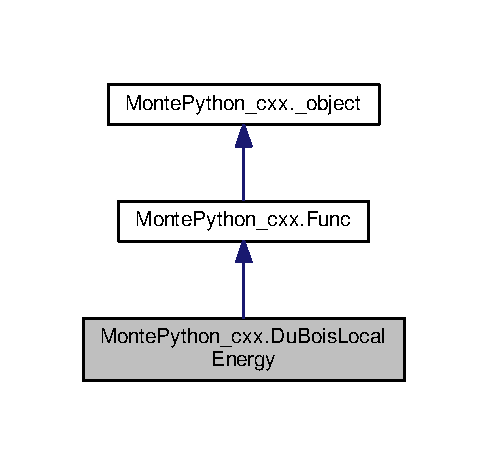
\includegraphics[width=234pt]{classMontePython__cxx_1_1DuBoisLocalEnergy__inherit__graph}
\end{center}
\end{figure}


Collaboration diagram for Monte\+Python\+\_\+cxx.\+Du\+Bois\+Local\+Energy\+:
\nopagebreak
\begin{figure}[H]
\begin{center}
\leavevmode
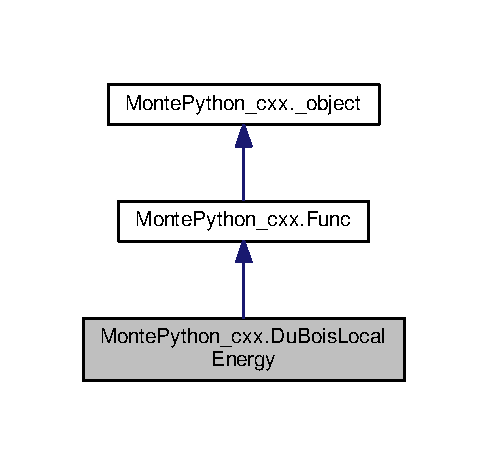
\includegraphics[width=234pt]{classMontePython__cxx_1_1DuBoisLocalEnergy__coll__graph}
\end{center}
\end{figure}
\subsection*{Public Member Functions}
\begin{DoxyCompactItemize}
\item 
def \hyperlink{classMontePython__cxx_1_1DuBoisLocalEnergy_a0fa0e1df9698e62f96778b3cbd504790}{set\+Params} (self, args)
\item 
def \hyperlink{classMontePython__cxx_1_1DuBoisLocalEnergy_a9f5f04aa78f658d43b17009c14eb08a2}{value\+Pt} (self, args)
\item 
def \hyperlink{classMontePython__cxx_1_1DuBoisLocalEnergy_a6a71340610d0b1c235b7b5416f641180}{\+\_\+\+\_\+call\+\_\+\+\_\+} (self, args)
\item 
def \hyperlink{classMontePython__cxx_1_1DuBoisLocalEnergy_af282e741ee21d335773fae1e1c9f89ca}{\+\_\+\+\_\+init\+\_\+\+\_\+} (self)
\end{DoxyCompactItemize}
\subsection*{Public Attributes}
\begin{DoxyCompactItemize}
\item 
\hypertarget{classMontePython__cxx_1_1DuBoisLocalEnergy_a4724180803d9e378a2af2cd9cf0451fb}{}{\bfseries this}\label{classMontePython__cxx_1_1DuBoisLocalEnergy_a4724180803d9e378a2af2cd9cf0451fb}

\end{DoxyCompactItemize}
\subsection*{Static Private Attributes}
\begin{DoxyCompactItemize}
\item 
\hypertarget{classMontePython__cxx_1_1DuBoisLocalEnergy_a026a8fdf942868dcc8c293dde56a7164}{}dictionary {\bfseries \+\_\+\+\_\+swig\+\_\+setmethods\+\_\+\+\_\+} = \{\}\label{classMontePython__cxx_1_1DuBoisLocalEnergy_a026a8fdf942868dcc8c293dde56a7164}

\item 
\hypertarget{classMontePython__cxx_1_1DuBoisLocalEnergy_aeb0e14f4c19454d0f9bcb58cb896d1c3}{}tuple {\bfseries \+\_\+\+\_\+setattr\+\_\+\+\_\+} = lambdaself,name,value\+:\+\_\+swig\+\_\+setattr(self, \hyperlink{classMontePython__cxx_1_1DuBoisLocalEnergy}{Du\+Bois\+Local\+Energy}, name, value)\label{classMontePython__cxx_1_1DuBoisLocalEnergy_aeb0e14f4c19454d0f9bcb58cb896d1c3}

\item 
\hypertarget{classMontePython__cxx_1_1DuBoisLocalEnergy_afecdf3a26668b8d0c96dfd7be2b3ebd5}{}dictionary {\bfseries \+\_\+\+\_\+swig\+\_\+getmethods\+\_\+\+\_\+} = \{\}\label{classMontePython__cxx_1_1DuBoisLocalEnergy_afecdf3a26668b8d0c96dfd7be2b3ebd5}

\item 
\hypertarget{classMontePython__cxx_1_1DuBoisLocalEnergy_ae83b82022753402dd25316798d745a77}{}tuple {\bfseries \+\_\+\+\_\+getattr\+\_\+\+\_\+} = lambdaself,name\+:\+\_\+swig\+\_\+getattr(self, \hyperlink{classMontePython__cxx_1_1DuBoisLocalEnergy}{Du\+Bois\+Local\+Energy}, name)\label{classMontePython__cxx_1_1DuBoisLocalEnergy_ae83b82022753402dd25316798d745a77}

\item 
\hypertarget{classMontePython__cxx_1_1DuBoisLocalEnergy_a7b302c1c515dd8a2ec0c85a034e2a7f5}{}{\bfseries \+\_\+\+\_\+repr\+\_\+\+\_\+} = \+\_\+swig\+\_\+repr\label{classMontePython__cxx_1_1DuBoisLocalEnergy_a7b302c1c515dd8a2ec0c85a034e2a7f5}

\item 
\hypertarget{classMontePython__cxx_1_1DuBoisLocalEnergy_ac5a0168d2572114752a9fc5bbdcd2e38}{}{\bfseries \+\_\+\+\_\+swig\+\_\+destroy\+\_\+\+\_\+} = \+\_\+\+Monte\+Python\+\_\+cxx.\+delete\+\_\+\+Du\+Bois\+Local\+Energy\label{classMontePython__cxx_1_1DuBoisLocalEnergy_ac5a0168d2572114752a9fc5bbdcd2e38}

\end{DoxyCompactItemize}


\subsection{Detailed Description}
\begin{DoxyVerb}Proxy of C++ DuBoisLocalEnergy class\end{DoxyVerb}
 

\subsection{Constructor \& Destructor Documentation}
\hypertarget{classMontePython__cxx_1_1DuBoisLocalEnergy_af282e741ee21d335773fae1e1c9f89ca}{}\index{Monte\+Python\+\_\+cxx\+::\+Du\+Bois\+Local\+Energy@{Monte\+Python\+\_\+cxx\+::\+Du\+Bois\+Local\+Energy}!\+\_\+\+\_\+init\+\_\+\+\_\+@{\+\_\+\+\_\+init\+\_\+\+\_\+}}
\index{\+\_\+\+\_\+init\+\_\+\+\_\+@{\+\_\+\+\_\+init\+\_\+\+\_\+}!Monte\+Python\+\_\+cxx\+::\+Du\+Bois\+Local\+Energy@{Monte\+Python\+\_\+cxx\+::\+Du\+Bois\+Local\+Energy}}
\subsubsection[{\+\_\+\+\_\+init\+\_\+\+\_\+}]{\setlength{\rightskip}{0pt plus 5cm}def Monte\+Python\+\_\+cxx.\+Du\+Bois\+Local\+Energy.\+\_\+\+\_\+init\+\_\+\+\_\+ (
\begin{DoxyParamCaption}
\item[{}]{self}
\end{DoxyParamCaption}
)}\label{classMontePython__cxx_1_1DuBoisLocalEnergy_af282e741ee21d335773fae1e1c9f89ca}
\begin{DoxyVerb}__init__(DuBoisLocalEnergy self) -> DuBoisLocalEnergy\end{DoxyVerb}
 

\subsection{Member Function Documentation}
\hypertarget{classMontePython__cxx_1_1DuBoisLocalEnergy_a6a71340610d0b1c235b7b5416f641180}{}\index{Monte\+Python\+\_\+cxx\+::\+Du\+Bois\+Local\+Energy@{Monte\+Python\+\_\+cxx\+::\+Du\+Bois\+Local\+Energy}!\+\_\+\+\_\+call\+\_\+\+\_\+@{\+\_\+\+\_\+call\+\_\+\+\_\+}}
\index{\+\_\+\+\_\+call\+\_\+\+\_\+@{\+\_\+\+\_\+call\+\_\+\+\_\+}!Monte\+Python\+\_\+cxx\+::\+Du\+Bois\+Local\+Energy@{Monte\+Python\+\_\+cxx\+::\+Du\+Bois\+Local\+Energy}}
\subsubsection[{\+\_\+\+\_\+call\+\_\+\+\_\+}]{\setlength{\rightskip}{0pt plus 5cm}def Monte\+Python\+\_\+cxx.\+Du\+Bois\+Local\+Energy.\+\_\+\+\_\+call\+\_\+\+\_\+ (
\begin{DoxyParamCaption}
\item[{}]{self, }
\item[{}]{args}
\end{DoxyParamCaption}
)}\label{classMontePython__cxx_1_1DuBoisLocalEnergy_a6a71340610d0b1c235b7b5416f641180}
\begin{DoxyVerb}__call__(DuBoisLocalEnergy self, QickArray & pos) -> double\end{DoxyVerb}
 \hypertarget{classMontePython__cxx_1_1DuBoisLocalEnergy_a0fa0e1df9698e62f96778b3cbd504790}{}\index{Monte\+Python\+\_\+cxx\+::\+Du\+Bois\+Local\+Energy@{Monte\+Python\+\_\+cxx\+::\+Du\+Bois\+Local\+Energy}!set\+Params@{set\+Params}}
\index{set\+Params@{set\+Params}!Monte\+Python\+\_\+cxx\+::\+Du\+Bois\+Local\+Energy@{Monte\+Python\+\_\+cxx\+::\+Du\+Bois\+Local\+Energy}}
\subsubsection[{set\+Params}]{\setlength{\rightskip}{0pt plus 5cm}def Monte\+Python\+\_\+cxx.\+Du\+Bois\+Local\+Energy.\+set\+Params (
\begin{DoxyParamCaption}
\item[{}]{self, }
\item[{}]{args}
\end{DoxyParamCaption}
)}\label{classMontePython__cxx_1_1DuBoisLocalEnergy_a0fa0e1df9698e62f96778b3cbd504790}
\begin{DoxyVerb}setParams(DuBoisLocalEnergy self, QickArray & params_)\end{DoxyVerb}
 \hypertarget{classMontePython__cxx_1_1DuBoisLocalEnergy_a9f5f04aa78f658d43b17009c14eb08a2}{}\index{Monte\+Python\+\_\+cxx\+::\+Du\+Bois\+Local\+Energy@{Monte\+Python\+\_\+cxx\+::\+Du\+Bois\+Local\+Energy}!value\+Pt@{value\+Pt}}
\index{value\+Pt@{value\+Pt}!Monte\+Python\+\_\+cxx\+::\+Du\+Bois\+Local\+Energy@{Monte\+Python\+\_\+cxx\+::\+Du\+Bois\+Local\+Energy}}
\subsubsection[{value\+Pt}]{\setlength{\rightskip}{0pt plus 5cm}def Monte\+Python\+\_\+cxx.\+Du\+Bois\+Local\+Energy.\+value\+Pt (
\begin{DoxyParamCaption}
\item[{}]{self, }
\item[{}]{args}
\end{DoxyParamCaption}
)}\label{classMontePython__cxx_1_1DuBoisLocalEnergy_a9f5f04aa78f658d43b17009c14eb08a2}
\begin{DoxyVerb}valuePt(DuBoisLocalEnergy self, QickArray & pos) -> double
valuePt(DuBoisLocalEnergy self, QickArray & pos, int dummy) -> double
\end{DoxyVerb}
 

The documentation for this class was generated from the following file\+:\begin{DoxyCompactItemize}
\item 
Monte\+Python\+\_\+cxx.\+py\end{DoxyCompactItemize}

\hypertarget{classMontePython__cxx_1_1DuBoisMove}{}\section{Monte\+Python\+\_\+cxx.\+Du\+Bois\+Move Class Reference}
\label{classMontePython__cxx_1_1DuBoisMove}\index{Monte\+Python\+\_\+cxx.\+Du\+Bois\+Move@{Monte\+Python\+\_\+cxx.\+Du\+Bois\+Move}}


Inheritance diagram for Monte\+Python\+\_\+cxx.\+Du\+Bois\+Move\+:
\nopagebreak
\begin{figure}[H]
\begin{center}
\leavevmode
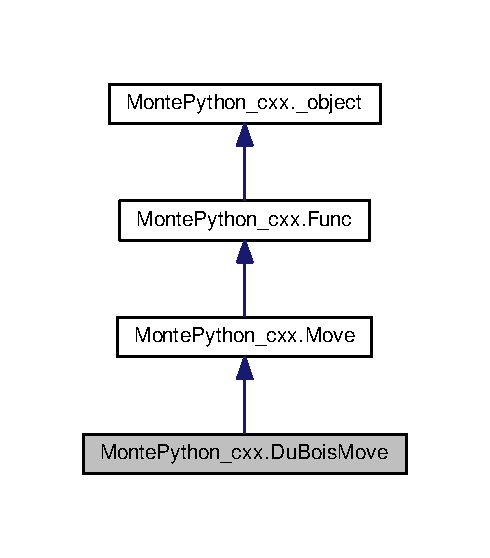
\includegraphics[width=235pt]{classMontePython__cxx_1_1DuBoisMove__inherit__graph}
\end{center}
\end{figure}


Collaboration diagram for Monte\+Python\+\_\+cxx.\+Du\+Bois\+Move\+:
\nopagebreak
\begin{figure}[H]
\begin{center}
\leavevmode
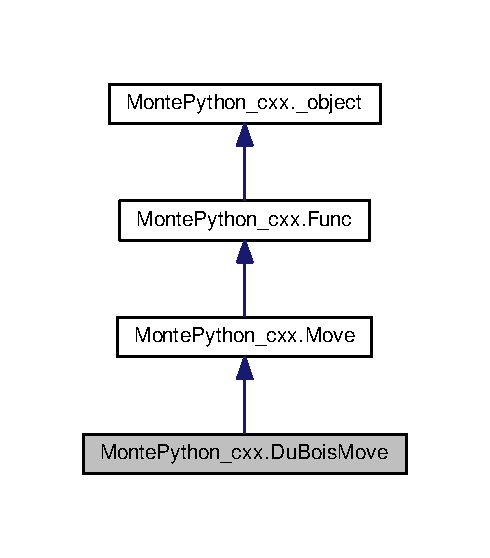
\includegraphics[width=235pt]{classMontePython__cxx_1_1DuBoisMove__coll__graph}
\end{center}
\end{figure}
\subsection*{Public Member Functions}
\begin{DoxyCompactItemize}
\item 
def \hyperlink{classMontePython__cxx_1_1DuBoisMove_ab3b73323c57aa0a66479dae8e27b06d9}{set\+Params} (self, args)
\item 
def \hyperlink{classMontePython__cxx_1_1DuBoisMove_a8d9585c1ea11c8c6499a46ae6e7969de}{get\+Impossible} (self)
\item 
def \hyperlink{classMontePython__cxx_1_1DuBoisMove_a3f32c1a72865be7daf007b84581df35b}{value\+Pt} (self, args)
\item 
def \hyperlink{classMontePython__cxx_1_1DuBoisMove_ac31ce48a51e59000a2157d017256ed8e}{\+\_\+\+\_\+call\+\_\+\+\_\+} (self, args)
\item 
def \hyperlink{classMontePython__cxx_1_1DuBoisMove_aa0c490502c79d926f45931805e87fb92}{\+\_\+\+\_\+init\+\_\+\+\_\+} (self)
\end{DoxyCompactItemize}
\subsection*{Public Attributes}
\begin{DoxyCompactItemize}
\item 
\hypertarget{classMontePython__cxx_1_1DuBoisMove_a39a08d500ea788acb71367af6f73db44}{}{\bfseries this}\label{classMontePython__cxx_1_1DuBoisMove_a39a08d500ea788acb71367af6f73db44}

\end{DoxyCompactItemize}
\subsection*{Static Private Attributes}
\begin{DoxyCompactItemize}
\item 
\hypertarget{classMontePython__cxx_1_1DuBoisMove_a7e1aad681435b4cda58621abef8081cf}{}dictionary {\bfseries \+\_\+\+\_\+swig\+\_\+setmethods\+\_\+\+\_\+} = \{\}\label{classMontePython__cxx_1_1DuBoisMove_a7e1aad681435b4cda58621abef8081cf}

\item 
\hypertarget{classMontePython__cxx_1_1DuBoisMove_a30e7ada4adb81be7a29ee08da8754d52}{}tuple {\bfseries \+\_\+\+\_\+setattr\+\_\+\+\_\+} = lambdaself,name,value\+:\+\_\+swig\+\_\+setattr(self, \hyperlink{classMontePython__cxx_1_1DuBoisMove}{Du\+Bois\+Move}, name, value)\label{classMontePython__cxx_1_1DuBoisMove_a30e7ada4adb81be7a29ee08da8754d52}

\item 
\hypertarget{classMontePython__cxx_1_1DuBoisMove_ab87a99207e02ec19bb2cfb389390a584}{}dictionary {\bfseries \+\_\+\+\_\+swig\+\_\+getmethods\+\_\+\+\_\+} = \{\}\label{classMontePython__cxx_1_1DuBoisMove_ab87a99207e02ec19bb2cfb389390a584}

\item 
\hypertarget{classMontePython__cxx_1_1DuBoisMove_a214d0ed1b400ce4fbd96b58fd6585140}{}tuple {\bfseries \+\_\+\+\_\+getattr\+\_\+\+\_\+} = lambdaself,name\+:\+\_\+swig\+\_\+getattr(self, \hyperlink{classMontePython__cxx_1_1DuBoisMove}{Du\+Bois\+Move}, name)\label{classMontePython__cxx_1_1DuBoisMove_a214d0ed1b400ce4fbd96b58fd6585140}

\item 
\hypertarget{classMontePython__cxx_1_1DuBoisMove_aef5801e3a8ed46391bfa3c76cc7ab62f}{}{\bfseries \+\_\+\+\_\+repr\+\_\+\+\_\+} = \+\_\+swig\+\_\+repr\label{classMontePython__cxx_1_1DuBoisMove_aef5801e3a8ed46391bfa3c76cc7ab62f}

\item 
\hypertarget{classMontePython__cxx_1_1DuBoisMove_a82ebfcd11327d4a7c2011195cd77e388}{}{\bfseries \+\_\+\+\_\+swig\+\_\+destroy\+\_\+\+\_\+} = \+\_\+\+Monte\+Python\+\_\+cxx.\+delete\+\_\+\+Du\+Bois\+Move\label{classMontePython__cxx_1_1DuBoisMove_a82ebfcd11327d4a7c2011195cd77e388}

\end{DoxyCompactItemize}


\subsection{Detailed Description}
\begin{DoxyVerb}Proxy of C++ DuBoisMove class\end{DoxyVerb}
 

\subsection{Constructor \& Destructor Documentation}
\hypertarget{classMontePython__cxx_1_1DuBoisMove_aa0c490502c79d926f45931805e87fb92}{}\index{Monte\+Python\+\_\+cxx\+::\+Du\+Bois\+Move@{Monte\+Python\+\_\+cxx\+::\+Du\+Bois\+Move}!\+\_\+\+\_\+init\+\_\+\+\_\+@{\+\_\+\+\_\+init\+\_\+\+\_\+}}
\index{\+\_\+\+\_\+init\+\_\+\+\_\+@{\+\_\+\+\_\+init\+\_\+\+\_\+}!Monte\+Python\+\_\+cxx\+::\+Du\+Bois\+Move@{Monte\+Python\+\_\+cxx\+::\+Du\+Bois\+Move}}
\subsubsection[{\+\_\+\+\_\+init\+\_\+\+\_\+}]{\setlength{\rightskip}{0pt plus 5cm}def Monte\+Python\+\_\+cxx.\+Du\+Bois\+Move.\+\_\+\+\_\+init\+\_\+\+\_\+ (
\begin{DoxyParamCaption}
\item[{}]{self}
\end{DoxyParamCaption}
)}\label{classMontePython__cxx_1_1DuBoisMove_aa0c490502c79d926f45931805e87fb92}
\begin{DoxyVerb}__init__(DuBoisMove self) -> DuBoisMove\end{DoxyVerb}
 

\subsection{Member Function Documentation}
\hypertarget{classMontePython__cxx_1_1DuBoisMove_ac31ce48a51e59000a2157d017256ed8e}{}\index{Monte\+Python\+\_\+cxx\+::\+Du\+Bois\+Move@{Monte\+Python\+\_\+cxx\+::\+Du\+Bois\+Move}!\+\_\+\+\_\+call\+\_\+\+\_\+@{\+\_\+\+\_\+call\+\_\+\+\_\+}}
\index{\+\_\+\+\_\+call\+\_\+\+\_\+@{\+\_\+\+\_\+call\+\_\+\+\_\+}!Monte\+Python\+\_\+cxx\+::\+Du\+Bois\+Move@{Monte\+Python\+\_\+cxx\+::\+Du\+Bois\+Move}}
\subsubsection[{\+\_\+\+\_\+call\+\_\+\+\_\+}]{\setlength{\rightskip}{0pt plus 5cm}def Monte\+Python\+\_\+cxx.\+Du\+Bois\+Move.\+\_\+\+\_\+call\+\_\+\+\_\+ (
\begin{DoxyParamCaption}
\item[{}]{self, }
\item[{}]{args}
\end{DoxyParamCaption}
)}\label{classMontePython__cxx_1_1DuBoisMove_ac31ce48a51e59000a2157d017256ed8e}
\begin{DoxyVerb}__call__(DuBoisMove self, QickArray & pos, int i, Random ran) -> QickArray
__call__(DuBoisMove self, QickArray & pos, int i, QickArray & x, Random ran) -> QickArray &
\end{DoxyVerb}
 \hypertarget{classMontePython__cxx_1_1DuBoisMove_a8d9585c1ea11c8c6499a46ae6e7969de}{}\index{Monte\+Python\+\_\+cxx\+::\+Du\+Bois\+Move@{Monte\+Python\+\_\+cxx\+::\+Du\+Bois\+Move}!get\+Impossible@{get\+Impossible}}
\index{get\+Impossible@{get\+Impossible}!Monte\+Python\+\_\+cxx\+::\+Du\+Bois\+Move@{Monte\+Python\+\_\+cxx\+::\+Du\+Bois\+Move}}
\subsubsection[{get\+Impossible}]{\setlength{\rightskip}{0pt plus 5cm}def Monte\+Python\+\_\+cxx.\+Du\+Bois\+Move.\+get\+Impossible (
\begin{DoxyParamCaption}
\item[{}]{self}
\end{DoxyParamCaption}
)}\label{classMontePython__cxx_1_1DuBoisMove_a8d9585c1ea11c8c6499a46ae6e7969de}
\begin{DoxyVerb}getImpossible(DuBoisMove self) -> bool\end{DoxyVerb}
 \hypertarget{classMontePython__cxx_1_1DuBoisMove_ab3b73323c57aa0a66479dae8e27b06d9}{}\index{Monte\+Python\+\_\+cxx\+::\+Du\+Bois\+Move@{Monte\+Python\+\_\+cxx\+::\+Du\+Bois\+Move}!set\+Params@{set\+Params}}
\index{set\+Params@{set\+Params}!Monte\+Python\+\_\+cxx\+::\+Du\+Bois\+Move@{Monte\+Python\+\_\+cxx\+::\+Du\+Bois\+Move}}
\subsubsection[{set\+Params}]{\setlength{\rightskip}{0pt plus 5cm}def Monte\+Python\+\_\+cxx.\+Du\+Bois\+Move.\+set\+Params (
\begin{DoxyParamCaption}
\item[{}]{self, }
\item[{}]{args}
\end{DoxyParamCaption}
)}\label{classMontePython__cxx_1_1DuBoisMove_ab3b73323c57aa0a66479dae8e27b06d9}
\begin{DoxyVerb}setParams(DuBoisMove self, QickArray & params_)\end{DoxyVerb}
 \hypertarget{classMontePython__cxx_1_1DuBoisMove_a3f32c1a72865be7daf007b84581df35b}{}\index{Monte\+Python\+\_\+cxx\+::\+Du\+Bois\+Move@{Monte\+Python\+\_\+cxx\+::\+Du\+Bois\+Move}!value\+Pt@{value\+Pt}}
\index{value\+Pt@{value\+Pt}!Monte\+Python\+\_\+cxx\+::\+Du\+Bois\+Move@{Monte\+Python\+\_\+cxx\+::\+Du\+Bois\+Move}}
\subsubsection[{value\+Pt}]{\setlength{\rightskip}{0pt plus 5cm}def Monte\+Python\+\_\+cxx.\+Du\+Bois\+Move.\+value\+Pt (
\begin{DoxyParamCaption}
\item[{}]{self, }
\item[{}]{args}
\end{DoxyParamCaption}
)}\label{classMontePython__cxx_1_1DuBoisMove_a3f32c1a72865be7daf007b84581df35b}
\begin{DoxyVerb}valuePt(DuBoisMove self, QickArray & pos, int i, Random ran) -> QickArray
valuePt(DuBoisMove self, QickArray & pos, int i, QickArray & x, Random ran) -> QickArray &
\end{DoxyVerb}
 

The documentation for this class was generated from the following file\+:\begin{DoxyCompactItemize}
\item 
Monte\+Python\+\_\+cxx.\+py\end{DoxyCompactItemize}

\hypertarget{classMontePython__cxx_1_1DuBoisPotentialEnergy}{}\section{Monte\+Python\+\_\+cxx.\+Du\+Bois\+Potential\+Energy Class Reference}
\label{classMontePython__cxx_1_1DuBoisPotentialEnergy}\index{Monte\+Python\+\_\+cxx.\+Du\+Bois\+Potential\+Energy@{Monte\+Python\+\_\+cxx.\+Du\+Bois\+Potential\+Energy}}


Inheritance diagram for Monte\+Python\+\_\+cxx.\+Du\+Bois\+Potential\+Energy\+:
\nopagebreak
\begin{figure}[H]
\begin{center}
\leavevmode
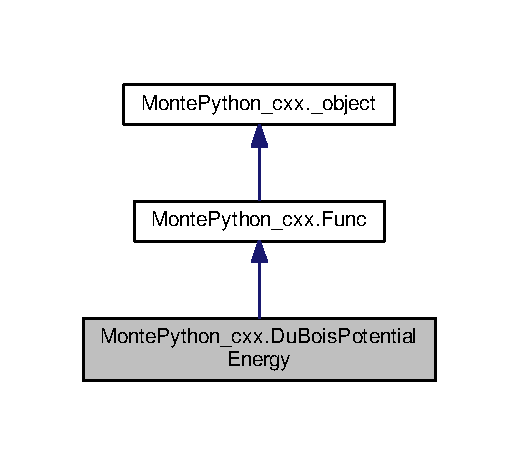
\includegraphics[width=249pt]{classMontePython__cxx_1_1DuBoisPotentialEnergy__inherit__graph}
\end{center}
\end{figure}


Collaboration diagram for Monte\+Python\+\_\+cxx.\+Du\+Bois\+Potential\+Energy\+:
\nopagebreak
\begin{figure}[H]
\begin{center}
\leavevmode
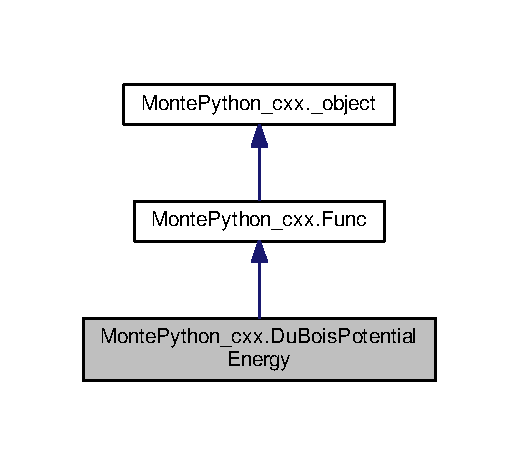
\includegraphics[width=249pt]{classMontePython__cxx_1_1DuBoisPotentialEnergy__coll__graph}
\end{center}
\end{figure}
\subsection*{Public Member Functions}
\begin{DoxyCompactItemize}
\item 
def \hyperlink{classMontePython__cxx_1_1DuBoisPotentialEnergy_a51ea3cb724a58cd53bf2627d0675ab77}{set\+Params} (self, args)
\item 
def \hyperlink{classMontePython__cxx_1_1DuBoisPotentialEnergy_a8f9a89b0411438ba0f5239ffbdefc989}{value\+Pt} (self, args)
\item 
def \hyperlink{classMontePython__cxx_1_1DuBoisPotentialEnergy_acadce239953113575c98b92cd10bfcfa}{\+\_\+\+\_\+call\+\_\+\+\_\+} (self, args)
\item 
def \hyperlink{classMontePython__cxx_1_1DuBoisPotentialEnergy_a42b758fe853e166f62a505d8ee5b77eb}{\+\_\+\+\_\+init\+\_\+\+\_\+} (self)
\end{DoxyCompactItemize}
\subsection*{Public Attributes}
\begin{DoxyCompactItemize}
\item 
\hypertarget{classMontePython__cxx_1_1DuBoisPotentialEnergy_a45cd5af8c1872c501d4b092e69ae11fb}{}{\bfseries this}\label{classMontePython__cxx_1_1DuBoisPotentialEnergy_a45cd5af8c1872c501d4b092e69ae11fb}

\end{DoxyCompactItemize}
\subsection*{Static Private Attributes}
\begin{DoxyCompactItemize}
\item 
\hypertarget{classMontePython__cxx_1_1DuBoisPotentialEnergy_ada69a71b53db57879a7dfd3165f64f6e}{}dictionary {\bfseries \+\_\+\+\_\+swig\+\_\+setmethods\+\_\+\+\_\+} = \{\}\label{classMontePython__cxx_1_1DuBoisPotentialEnergy_ada69a71b53db57879a7dfd3165f64f6e}

\item 
\hypertarget{classMontePython__cxx_1_1DuBoisPotentialEnergy_a1d89f790e102b695f5c009cd2f5e9e6e}{}tuple {\bfseries \+\_\+\+\_\+setattr\+\_\+\+\_\+} = lambdaself,name,value\+:\+\_\+swig\+\_\+setattr(self, \hyperlink{classMontePython__cxx_1_1DuBoisPotentialEnergy}{Du\+Bois\+Potential\+Energy}, name, value)\label{classMontePython__cxx_1_1DuBoisPotentialEnergy_a1d89f790e102b695f5c009cd2f5e9e6e}

\item 
\hypertarget{classMontePython__cxx_1_1DuBoisPotentialEnergy_a3d4f8a747638b8d6e7621c11d788994a}{}dictionary {\bfseries \+\_\+\+\_\+swig\+\_\+getmethods\+\_\+\+\_\+} = \{\}\label{classMontePython__cxx_1_1DuBoisPotentialEnergy_a3d4f8a747638b8d6e7621c11d788994a}

\item 
\hypertarget{classMontePython__cxx_1_1DuBoisPotentialEnergy_a20c7ceb0e44360647823cccf022ae68f}{}tuple {\bfseries \+\_\+\+\_\+getattr\+\_\+\+\_\+} = lambdaself,name\+:\+\_\+swig\+\_\+getattr(self, \hyperlink{classMontePython__cxx_1_1DuBoisPotentialEnergy}{Du\+Bois\+Potential\+Energy}, name)\label{classMontePython__cxx_1_1DuBoisPotentialEnergy_a20c7ceb0e44360647823cccf022ae68f}

\item 
\hypertarget{classMontePython__cxx_1_1DuBoisPotentialEnergy_a16b959379f4753ebb27e814a45dbed72}{}{\bfseries \+\_\+\+\_\+repr\+\_\+\+\_\+} = \+\_\+swig\+\_\+repr\label{classMontePython__cxx_1_1DuBoisPotentialEnergy_a16b959379f4753ebb27e814a45dbed72}

\item 
\hypertarget{classMontePython__cxx_1_1DuBoisPotentialEnergy_ac8db1e7f07c3730024bc87bdf8d152f3}{}{\bfseries \+\_\+\+\_\+swig\+\_\+destroy\+\_\+\+\_\+} = \+\_\+\+Monte\+Python\+\_\+cxx.\+delete\+\_\+\+Du\+Bois\+Potential\+Energy\label{classMontePython__cxx_1_1DuBoisPotentialEnergy_ac8db1e7f07c3730024bc87bdf8d152f3}

\end{DoxyCompactItemize}


\subsection{Detailed Description}
\begin{DoxyVerb}Proxy of C++ DuBoisPotentialEnergy class\end{DoxyVerb}
 

\subsection{Constructor \& Destructor Documentation}
\hypertarget{classMontePython__cxx_1_1DuBoisPotentialEnergy_a42b758fe853e166f62a505d8ee5b77eb}{}\index{Monte\+Python\+\_\+cxx\+::\+Du\+Bois\+Potential\+Energy@{Monte\+Python\+\_\+cxx\+::\+Du\+Bois\+Potential\+Energy}!\+\_\+\+\_\+init\+\_\+\+\_\+@{\+\_\+\+\_\+init\+\_\+\+\_\+}}
\index{\+\_\+\+\_\+init\+\_\+\+\_\+@{\+\_\+\+\_\+init\+\_\+\+\_\+}!Monte\+Python\+\_\+cxx\+::\+Du\+Bois\+Potential\+Energy@{Monte\+Python\+\_\+cxx\+::\+Du\+Bois\+Potential\+Energy}}
\subsubsection[{\+\_\+\+\_\+init\+\_\+\+\_\+}]{\setlength{\rightskip}{0pt plus 5cm}def Monte\+Python\+\_\+cxx.\+Du\+Bois\+Potential\+Energy.\+\_\+\+\_\+init\+\_\+\+\_\+ (
\begin{DoxyParamCaption}
\item[{}]{self}
\end{DoxyParamCaption}
)}\label{classMontePython__cxx_1_1DuBoisPotentialEnergy_a42b758fe853e166f62a505d8ee5b77eb}
\begin{DoxyVerb}__init__(DuBoisPotentialEnergy self) -> DuBoisPotentialEnergy\end{DoxyVerb}
 

\subsection{Member Function Documentation}
\hypertarget{classMontePython__cxx_1_1DuBoisPotentialEnergy_acadce239953113575c98b92cd10bfcfa}{}\index{Monte\+Python\+\_\+cxx\+::\+Du\+Bois\+Potential\+Energy@{Monte\+Python\+\_\+cxx\+::\+Du\+Bois\+Potential\+Energy}!\+\_\+\+\_\+call\+\_\+\+\_\+@{\+\_\+\+\_\+call\+\_\+\+\_\+}}
\index{\+\_\+\+\_\+call\+\_\+\+\_\+@{\+\_\+\+\_\+call\+\_\+\+\_\+}!Monte\+Python\+\_\+cxx\+::\+Du\+Bois\+Potential\+Energy@{Monte\+Python\+\_\+cxx\+::\+Du\+Bois\+Potential\+Energy}}
\subsubsection[{\+\_\+\+\_\+call\+\_\+\+\_\+}]{\setlength{\rightskip}{0pt plus 5cm}def Monte\+Python\+\_\+cxx.\+Du\+Bois\+Potential\+Energy.\+\_\+\+\_\+call\+\_\+\+\_\+ (
\begin{DoxyParamCaption}
\item[{}]{self, }
\item[{}]{args}
\end{DoxyParamCaption}
)}\label{classMontePython__cxx_1_1DuBoisPotentialEnergy_acadce239953113575c98b92cd10bfcfa}
\begin{DoxyVerb}__call__(DuBoisPotentialEnergy self, QickArray & pos) -> double\end{DoxyVerb}
 \hypertarget{classMontePython__cxx_1_1DuBoisPotentialEnergy_a51ea3cb724a58cd53bf2627d0675ab77}{}\index{Monte\+Python\+\_\+cxx\+::\+Du\+Bois\+Potential\+Energy@{Monte\+Python\+\_\+cxx\+::\+Du\+Bois\+Potential\+Energy}!set\+Params@{set\+Params}}
\index{set\+Params@{set\+Params}!Monte\+Python\+\_\+cxx\+::\+Du\+Bois\+Potential\+Energy@{Monte\+Python\+\_\+cxx\+::\+Du\+Bois\+Potential\+Energy}}
\subsubsection[{set\+Params}]{\setlength{\rightskip}{0pt plus 5cm}def Monte\+Python\+\_\+cxx.\+Du\+Bois\+Potential\+Energy.\+set\+Params (
\begin{DoxyParamCaption}
\item[{}]{self, }
\item[{}]{args}
\end{DoxyParamCaption}
)}\label{classMontePython__cxx_1_1DuBoisPotentialEnergy_a51ea3cb724a58cd53bf2627d0675ab77}
\begin{DoxyVerb}setParams(DuBoisPotentialEnergy self, QickArray & params_)\end{DoxyVerb}
 \hypertarget{classMontePython__cxx_1_1DuBoisPotentialEnergy_a8f9a89b0411438ba0f5239ffbdefc989}{}\index{Monte\+Python\+\_\+cxx\+::\+Du\+Bois\+Potential\+Energy@{Monte\+Python\+\_\+cxx\+::\+Du\+Bois\+Potential\+Energy}!value\+Pt@{value\+Pt}}
\index{value\+Pt@{value\+Pt}!Monte\+Python\+\_\+cxx\+::\+Du\+Bois\+Potential\+Energy@{Monte\+Python\+\_\+cxx\+::\+Du\+Bois\+Potential\+Energy}}
\subsubsection[{value\+Pt}]{\setlength{\rightskip}{0pt plus 5cm}def Monte\+Python\+\_\+cxx.\+Du\+Bois\+Potential\+Energy.\+value\+Pt (
\begin{DoxyParamCaption}
\item[{}]{self, }
\item[{}]{args}
\end{DoxyParamCaption}
)}\label{classMontePython__cxx_1_1DuBoisPotentialEnergy_a8f9a89b0411438ba0f5239ffbdefc989}
\begin{DoxyVerb}valuePt(DuBoisPotentialEnergy self, QickArray & pos) -> double\end{DoxyVerb}
 

The documentation for this class was generated from the following file\+:\begin{DoxyCompactItemize}
\item 
Monte\+Python\+\_\+cxx.\+py\end{DoxyCompactItemize}

\hypertarget{classMontePython__cxx_1_1DuBoisQForce}{}\section{Monte\+Python\+\_\+cxx.\+Du\+Bois\+Q\+Force Class Reference}
\label{classMontePython__cxx_1_1DuBoisQForce}\index{Monte\+Python\+\_\+cxx.\+Du\+Bois\+Q\+Force@{Monte\+Python\+\_\+cxx.\+Du\+Bois\+Q\+Force}}


Inheritance diagram for Monte\+Python\+\_\+cxx.\+Du\+Bois\+Q\+Force\+:
\nopagebreak
\begin{figure}[H]
\begin{center}
\leavevmode
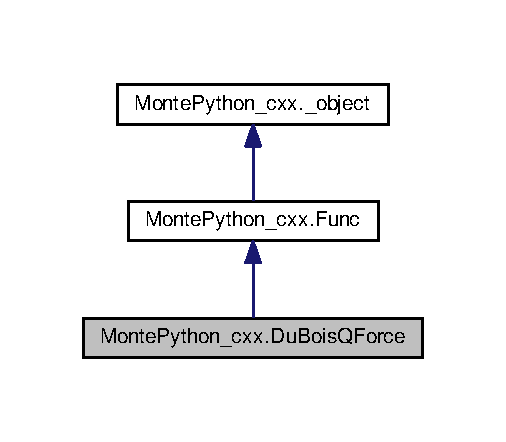
\includegraphics[width=243pt]{classMontePython__cxx_1_1DuBoisQForce__inherit__graph}
\end{center}
\end{figure}


Collaboration diagram for Monte\+Python\+\_\+cxx.\+Du\+Bois\+Q\+Force\+:
\nopagebreak
\begin{figure}[H]
\begin{center}
\leavevmode
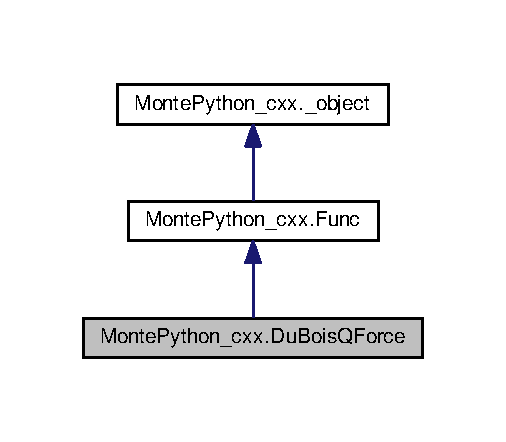
\includegraphics[width=243pt]{classMontePython__cxx_1_1DuBoisQForce__coll__graph}
\end{center}
\end{figure}
\subsection*{Public Member Functions}
\begin{DoxyCompactItemize}
\item 
def \hyperlink{classMontePython__cxx_1_1DuBoisQForce_a89366df1d55c80fc49a0950a5a1c6fce}{set\+Params} (self, args)
\item 
def \hyperlink{classMontePython__cxx_1_1DuBoisQForce_a03e6a2a7e2ce522eb78020bf020eb069}{value\+Pt} (self, args)
\item 
def \hyperlink{classMontePython__cxx_1_1DuBoisQForce_a01be349a65fa2100ec0cd7346367747e}{\+\_\+\+\_\+call\+\_\+\+\_\+} (self, args)
\item 
def \hyperlink{classMontePython__cxx_1_1DuBoisQForce_a869a270084ee136dc146a240098a66a9}{\+\_\+\+\_\+init\+\_\+\+\_\+} (self)
\end{DoxyCompactItemize}
\subsection*{Public Attributes}
\begin{DoxyCompactItemize}
\item 
\hypertarget{classMontePython__cxx_1_1DuBoisQForce_a3f40a8e403f06d8306ed7da8d48e1ffc}{}{\bfseries this}\label{classMontePython__cxx_1_1DuBoisQForce_a3f40a8e403f06d8306ed7da8d48e1ffc}

\end{DoxyCompactItemize}
\subsection*{Static Private Attributes}
\begin{DoxyCompactItemize}
\item 
\hypertarget{classMontePython__cxx_1_1DuBoisQForce_a4722237d210ece6a5609f2f1e2cd412c}{}dictionary {\bfseries \+\_\+\+\_\+swig\+\_\+setmethods\+\_\+\+\_\+} = \{\}\label{classMontePython__cxx_1_1DuBoisQForce_a4722237d210ece6a5609f2f1e2cd412c}

\item 
\hypertarget{classMontePython__cxx_1_1DuBoisQForce_a1bbca8bf0dc1faa110b1c94d6689fda0}{}tuple {\bfseries \+\_\+\+\_\+setattr\+\_\+\+\_\+} = lambdaself,name,value\+:\+\_\+swig\+\_\+setattr(self, \hyperlink{classMontePython__cxx_1_1DuBoisQForce}{Du\+Bois\+Q\+Force}, name, value)\label{classMontePython__cxx_1_1DuBoisQForce_a1bbca8bf0dc1faa110b1c94d6689fda0}

\item 
\hypertarget{classMontePython__cxx_1_1DuBoisQForce_a4729c24f8df144e0ec808588a71cf7de}{}dictionary {\bfseries \+\_\+\+\_\+swig\+\_\+getmethods\+\_\+\+\_\+} = \{\}\label{classMontePython__cxx_1_1DuBoisQForce_a4729c24f8df144e0ec808588a71cf7de}

\item 
\hypertarget{classMontePython__cxx_1_1DuBoisQForce_aee6b184b8cd1bc24c3c1fe65b5495685}{}tuple {\bfseries \+\_\+\+\_\+getattr\+\_\+\+\_\+} = lambdaself,name\+:\+\_\+swig\+\_\+getattr(self, \hyperlink{classMontePython__cxx_1_1DuBoisQForce}{Du\+Bois\+Q\+Force}, name)\label{classMontePython__cxx_1_1DuBoisQForce_aee6b184b8cd1bc24c3c1fe65b5495685}

\item 
\hypertarget{classMontePython__cxx_1_1DuBoisQForce_a3ecf8259c4038f63dcf6d7e8826c50ef}{}{\bfseries \+\_\+\+\_\+repr\+\_\+\+\_\+} = \+\_\+swig\+\_\+repr\label{classMontePython__cxx_1_1DuBoisQForce_a3ecf8259c4038f63dcf6d7e8826c50ef}

\item 
\hypertarget{classMontePython__cxx_1_1DuBoisQForce_a712d3a0166664e6320e4e779ee23da53}{}{\bfseries \+\_\+\+\_\+swig\+\_\+destroy\+\_\+\+\_\+} = \+\_\+\+Monte\+Python\+\_\+cxx.\+delete\+\_\+\+Du\+Bois\+Q\+Force\label{classMontePython__cxx_1_1DuBoisQForce_a712d3a0166664e6320e4e779ee23da53}

\end{DoxyCompactItemize}


\subsection{Detailed Description}
\begin{DoxyVerb}Proxy of C++ DuBoisQForce class\end{DoxyVerb}
 

\subsection{Constructor \& Destructor Documentation}
\hypertarget{classMontePython__cxx_1_1DuBoisQForce_a869a270084ee136dc146a240098a66a9}{}\index{Monte\+Python\+\_\+cxx\+::\+Du\+Bois\+Q\+Force@{Monte\+Python\+\_\+cxx\+::\+Du\+Bois\+Q\+Force}!\+\_\+\+\_\+init\+\_\+\+\_\+@{\+\_\+\+\_\+init\+\_\+\+\_\+}}
\index{\+\_\+\+\_\+init\+\_\+\+\_\+@{\+\_\+\+\_\+init\+\_\+\+\_\+}!Monte\+Python\+\_\+cxx\+::\+Du\+Bois\+Q\+Force@{Monte\+Python\+\_\+cxx\+::\+Du\+Bois\+Q\+Force}}
\subsubsection[{\+\_\+\+\_\+init\+\_\+\+\_\+}]{\setlength{\rightskip}{0pt plus 5cm}def Monte\+Python\+\_\+cxx.\+Du\+Bois\+Q\+Force.\+\_\+\+\_\+init\+\_\+\+\_\+ (
\begin{DoxyParamCaption}
\item[{}]{self}
\end{DoxyParamCaption}
)}\label{classMontePython__cxx_1_1DuBoisQForce_a869a270084ee136dc146a240098a66a9}
\begin{DoxyVerb}__init__(DuBoisQForce self) -> DuBoisQForce\end{DoxyVerb}
 

\subsection{Member Function Documentation}
\hypertarget{classMontePython__cxx_1_1DuBoisQForce_a01be349a65fa2100ec0cd7346367747e}{}\index{Monte\+Python\+\_\+cxx\+::\+Du\+Bois\+Q\+Force@{Monte\+Python\+\_\+cxx\+::\+Du\+Bois\+Q\+Force}!\+\_\+\+\_\+call\+\_\+\+\_\+@{\+\_\+\+\_\+call\+\_\+\+\_\+}}
\index{\+\_\+\+\_\+call\+\_\+\+\_\+@{\+\_\+\+\_\+call\+\_\+\+\_\+}!Monte\+Python\+\_\+cxx\+::\+Du\+Bois\+Q\+Force@{Monte\+Python\+\_\+cxx\+::\+Du\+Bois\+Q\+Force}}
\subsubsection[{\+\_\+\+\_\+call\+\_\+\+\_\+}]{\setlength{\rightskip}{0pt plus 5cm}def Monte\+Python\+\_\+cxx.\+Du\+Bois\+Q\+Force.\+\_\+\+\_\+call\+\_\+\+\_\+ (
\begin{DoxyParamCaption}
\item[{}]{self, }
\item[{}]{args}
\end{DoxyParamCaption}
)}\label{classMontePython__cxx_1_1DuBoisQForce_a01be349a65fa2100ec0cd7346367747e}
\begin{DoxyVerb}__call__(DuBoisQForce self, QickArray & pos, bool dummy) -> QickArray &\end{DoxyVerb}
 \hypertarget{classMontePython__cxx_1_1DuBoisQForce_a89366df1d55c80fc49a0950a5a1c6fce}{}\index{Monte\+Python\+\_\+cxx\+::\+Du\+Bois\+Q\+Force@{Monte\+Python\+\_\+cxx\+::\+Du\+Bois\+Q\+Force}!set\+Params@{set\+Params}}
\index{set\+Params@{set\+Params}!Monte\+Python\+\_\+cxx\+::\+Du\+Bois\+Q\+Force@{Monte\+Python\+\_\+cxx\+::\+Du\+Bois\+Q\+Force}}
\subsubsection[{set\+Params}]{\setlength{\rightskip}{0pt plus 5cm}def Monte\+Python\+\_\+cxx.\+Du\+Bois\+Q\+Force.\+set\+Params (
\begin{DoxyParamCaption}
\item[{}]{self, }
\item[{}]{args}
\end{DoxyParamCaption}
)}\label{classMontePython__cxx_1_1DuBoisQForce_a89366df1d55c80fc49a0950a5a1c6fce}
\begin{DoxyVerb}setParams(DuBoisQForce self, QickArray & params_)\end{DoxyVerb}
 \hypertarget{classMontePython__cxx_1_1DuBoisQForce_a03e6a2a7e2ce522eb78020bf020eb069}{}\index{Monte\+Python\+\_\+cxx\+::\+Du\+Bois\+Q\+Force@{Monte\+Python\+\_\+cxx\+::\+Du\+Bois\+Q\+Force}!value\+Pt@{value\+Pt}}
\index{value\+Pt@{value\+Pt}!Monte\+Python\+\_\+cxx\+::\+Du\+Bois\+Q\+Force@{Monte\+Python\+\_\+cxx\+::\+Du\+Bois\+Q\+Force}}
\subsubsection[{value\+Pt}]{\setlength{\rightskip}{0pt plus 5cm}def Monte\+Python\+\_\+cxx.\+Du\+Bois\+Q\+Force.\+value\+Pt (
\begin{DoxyParamCaption}
\item[{}]{self, }
\item[{}]{args}
\end{DoxyParamCaption}
)}\label{classMontePython__cxx_1_1DuBoisQForce_a03e6a2a7e2ce522eb78020bf020eb069}
\begin{DoxyVerb}valuePt(DuBoisQForce self, QickArray & pos, bool dummy) -> QickArray &\end{DoxyVerb}
 

The documentation for this class was generated from the following file\+:\begin{DoxyCompactItemize}
\item 
Monte\+Python\+\_\+cxx.\+py\end{DoxyCompactItemize}

\hypertarget{classMontePython__cxx_1_1DuBoisVortexExcitationEnergy}{}\section{Monte\+Python\+\_\+cxx.\+Du\+Bois\+Vortex\+Excitation\+Energy Class Reference}
\label{classMontePython__cxx_1_1DuBoisVortexExcitationEnergy}\index{Monte\+Python\+\_\+cxx.\+Du\+Bois\+Vortex\+Excitation\+Energy@{Monte\+Python\+\_\+cxx.\+Du\+Bois\+Vortex\+Excitation\+Energy}}


Inheritance diagram for Monte\+Python\+\_\+cxx.\+Du\+Bois\+Vortex\+Excitation\+Energy\+:
\nopagebreak
\begin{figure}[H]
\begin{center}
\leavevmode
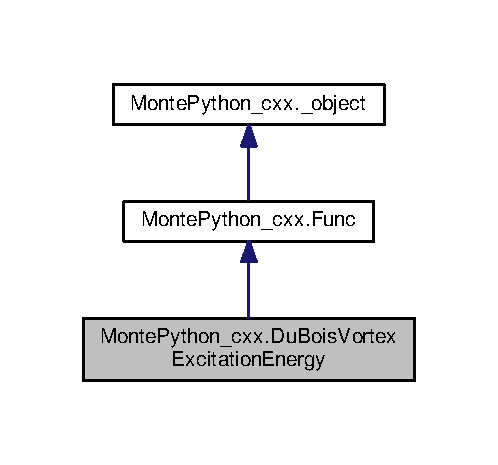
\includegraphics[width=239pt]{classMontePython__cxx_1_1DuBoisVortexExcitationEnergy__inherit__graph}
\end{center}
\end{figure}


Collaboration diagram for Monte\+Python\+\_\+cxx.\+Du\+Bois\+Vortex\+Excitation\+Energy\+:
\nopagebreak
\begin{figure}[H]
\begin{center}
\leavevmode
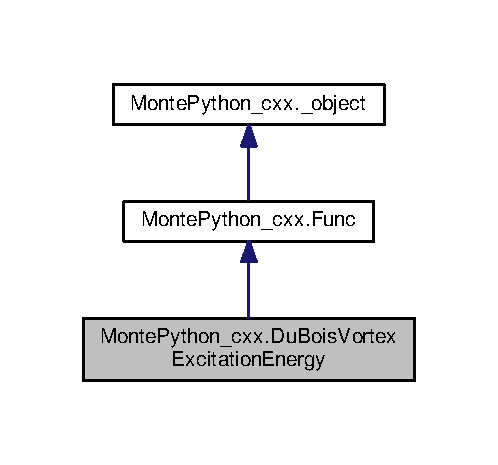
\includegraphics[width=239pt]{classMontePython__cxx_1_1DuBoisVortexExcitationEnergy__coll__graph}
\end{center}
\end{figure}
\subsection*{Public Member Functions}
\begin{DoxyCompactItemize}
\item 
def \hyperlink{classMontePython__cxx_1_1DuBoisVortexExcitationEnergy_a129a46d52b427cf4f8f5007567351b6e}{set\+Params} (self, args)
\item 
def \hyperlink{classMontePython__cxx_1_1DuBoisVortexExcitationEnergy_a50689e5140009be1b1eacbedf61b7fac}{value\+Pt} (self, args)
\item 
def \hyperlink{classMontePython__cxx_1_1DuBoisVortexExcitationEnergy_a290f18baa47ff46ff023747a0286f9b1}{\+\_\+\+\_\+call\+\_\+\+\_\+} (self, args)
\item 
def \hyperlink{classMontePython__cxx_1_1DuBoisVortexExcitationEnergy_aee334159a1bcd20f91a3bfb333eafc4f}{\+\_\+\+\_\+init\+\_\+\+\_\+} (self)
\end{DoxyCompactItemize}
\subsection*{Public Attributes}
\begin{DoxyCompactItemize}
\item 
\hypertarget{classMontePython__cxx_1_1DuBoisVortexExcitationEnergy_ae6b5b40dd7a72cacadb9b1c70131f781}{}{\bfseries this}\label{classMontePython__cxx_1_1DuBoisVortexExcitationEnergy_ae6b5b40dd7a72cacadb9b1c70131f781}

\end{DoxyCompactItemize}
\subsection*{Static Private Attributes}
\begin{DoxyCompactItemize}
\item 
\hypertarget{classMontePython__cxx_1_1DuBoisVortexExcitationEnergy_abed192bab3bd2b9345319225c3a7468b}{}dictionary {\bfseries \+\_\+\+\_\+swig\+\_\+setmethods\+\_\+\+\_\+} = \{\}\label{classMontePython__cxx_1_1DuBoisVortexExcitationEnergy_abed192bab3bd2b9345319225c3a7468b}

\item 
\hypertarget{classMontePython__cxx_1_1DuBoisVortexExcitationEnergy_a61b6a66ee7109173f31a611efa78af9d}{}tuple {\bfseries \+\_\+\+\_\+setattr\+\_\+\+\_\+} = lambdaself,name,value\+:\+\_\+swig\+\_\+setattr(self, \hyperlink{classMontePython__cxx_1_1DuBoisVortexExcitationEnergy}{Du\+Bois\+Vortex\+Excitation\+Energy}, name, value)\label{classMontePython__cxx_1_1DuBoisVortexExcitationEnergy_a61b6a66ee7109173f31a611efa78af9d}

\item 
\hypertarget{classMontePython__cxx_1_1DuBoisVortexExcitationEnergy_aed6bc35f821f78ebdebc558d0d5d47a8}{}dictionary {\bfseries \+\_\+\+\_\+swig\+\_\+getmethods\+\_\+\+\_\+} = \{\}\label{classMontePython__cxx_1_1DuBoisVortexExcitationEnergy_aed6bc35f821f78ebdebc558d0d5d47a8}

\item 
\hypertarget{classMontePython__cxx_1_1DuBoisVortexExcitationEnergy_a20f18564b2f2b2e2a17f24275ce4ffa6}{}tuple {\bfseries \+\_\+\+\_\+getattr\+\_\+\+\_\+} = lambdaself,name\+:\+\_\+swig\+\_\+getattr(self, \hyperlink{classMontePython__cxx_1_1DuBoisVortexExcitationEnergy}{Du\+Bois\+Vortex\+Excitation\+Energy}, name)\label{classMontePython__cxx_1_1DuBoisVortexExcitationEnergy_a20f18564b2f2b2e2a17f24275ce4ffa6}

\item 
\hypertarget{classMontePython__cxx_1_1DuBoisVortexExcitationEnergy_a323733b48132e7921b272eada09a6695}{}{\bfseries \+\_\+\+\_\+repr\+\_\+\+\_\+} = \+\_\+swig\+\_\+repr\label{classMontePython__cxx_1_1DuBoisVortexExcitationEnergy_a323733b48132e7921b272eada09a6695}

\item 
\hypertarget{classMontePython__cxx_1_1DuBoisVortexExcitationEnergy_a469f0a35a04fa57db76d4ae194b16168}{}{\bfseries \+\_\+\+\_\+swig\+\_\+destroy\+\_\+\+\_\+} = \+\_\+\+Monte\+Python\+\_\+cxx.\+delete\+\_\+\+Du\+Bois\+Vortex\+Excitation\+Energy\label{classMontePython__cxx_1_1DuBoisVortexExcitationEnergy_a469f0a35a04fa57db76d4ae194b16168}

\end{DoxyCompactItemize}


\subsection{Detailed Description}
\begin{DoxyVerb}Proxy of C++ DuBoisVortexExcitationEnergy class\end{DoxyVerb}
 

\subsection{Constructor \& Destructor Documentation}
\hypertarget{classMontePython__cxx_1_1DuBoisVortexExcitationEnergy_aee334159a1bcd20f91a3bfb333eafc4f}{}\index{Monte\+Python\+\_\+cxx\+::\+Du\+Bois\+Vortex\+Excitation\+Energy@{Monte\+Python\+\_\+cxx\+::\+Du\+Bois\+Vortex\+Excitation\+Energy}!\+\_\+\+\_\+init\+\_\+\+\_\+@{\+\_\+\+\_\+init\+\_\+\+\_\+}}
\index{\+\_\+\+\_\+init\+\_\+\+\_\+@{\+\_\+\+\_\+init\+\_\+\+\_\+}!Monte\+Python\+\_\+cxx\+::\+Du\+Bois\+Vortex\+Excitation\+Energy@{Monte\+Python\+\_\+cxx\+::\+Du\+Bois\+Vortex\+Excitation\+Energy}}
\subsubsection[{\+\_\+\+\_\+init\+\_\+\+\_\+}]{\setlength{\rightskip}{0pt plus 5cm}def Monte\+Python\+\_\+cxx.\+Du\+Bois\+Vortex\+Excitation\+Energy.\+\_\+\+\_\+init\+\_\+\+\_\+ (
\begin{DoxyParamCaption}
\item[{}]{self}
\end{DoxyParamCaption}
)}\label{classMontePython__cxx_1_1DuBoisVortexExcitationEnergy_aee334159a1bcd20f91a3bfb333eafc4f}
\begin{DoxyVerb}__init__(DuBoisVortexExcitationEnergy self) -> DuBoisVortexExcitationEnergy\end{DoxyVerb}
 

\subsection{Member Function Documentation}
\hypertarget{classMontePython__cxx_1_1DuBoisVortexExcitationEnergy_a290f18baa47ff46ff023747a0286f9b1}{}\index{Monte\+Python\+\_\+cxx\+::\+Du\+Bois\+Vortex\+Excitation\+Energy@{Monte\+Python\+\_\+cxx\+::\+Du\+Bois\+Vortex\+Excitation\+Energy}!\+\_\+\+\_\+call\+\_\+\+\_\+@{\+\_\+\+\_\+call\+\_\+\+\_\+}}
\index{\+\_\+\+\_\+call\+\_\+\+\_\+@{\+\_\+\+\_\+call\+\_\+\+\_\+}!Monte\+Python\+\_\+cxx\+::\+Du\+Bois\+Vortex\+Excitation\+Energy@{Monte\+Python\+\_\+cxx\+::\+Du\+Bois\+Vortex\+Excitation\+Energy}}
\subsubsection[{\+\_\+\+\_\+call\+\_\+\+\_\+}]{\setlength{\rightskip}{0pt plus 5cm}def Monte\+Python\+\_\+cxx.\+Du\+Bois\+Vortex\+Excitation\+Energy.\+\_\+\+\_\+call\+\_\+\+\_\+ (
\begin{DoxyParamCaption}
\item[{}]{self, }
\item[{}]{args}
\end{DoxyParamCaption}
)}\label{classMontePython__cxx_1_1DuBoisVortexExcitationEnergy_a290f18baa47ff46ff023747a0286f9b1}
\begin{DoxyVerb}__call__(DuBoisVortexExcitationEnergy self, QickArray & pos) -> double\end{DoxyVerb}
 \hypertarget{classMontePython__cxx_1_1DuBoisVortexExcitationEnergy_a129a46d52b427cf4f8f5007567351b6e}{}\index{Monte\+Python\+\_\+cxx\+::\+Du\+Bois\+Vortex\+Excitation\+Energy@{Monte\+Python\+\_\+cxx\+::\+Du\+Bois\+Vortex\+Excitation\+Energy}!set\+Params@{set\+Params}}
\index{set\+Params@{set\+Params}!Monte\+Python\+\_\+cxx\+::\+Du\+Bois\+Vortex\+Excitation\+Energy@{Monte\+Python\+\_\+cxx\+::\+Du\+Bois\+Vortex\+Excitation\+Energy}}
\subsubsection[{set\+Params}]{\setlength{\rightskip}{0pt plus 5cm}def Monte\+Python\+\_\+cxx.\+Du\+Bois\+Vortex\+Excitation\+Energy.\+set\+Params (
\begin{DoxyParamCaption}
\item[{}]{self, }
\item[{}]{args}
\end{DoxyParamCaption}
)}\label{classMontePython__cxx_1_1DuBoisVortexExcitationEnergy_a129a46d52b427cf4f8f5007567351b6e}
\begin{DoxyVerb}setParams(DuBoisVortexExcitationEnergy self, QickArray & params_)\end{DoxyVerb}
 \hypertarget{classMontePython__cxx_1_1DuBoisVortexExcitationEnergy_a50689e5140009be1b1eacbedf61b7fac}{}\index{Monte\+Python\+\_\+cxx\+::\+Du\+Bois\+Vortex\+Excitation\+Energy@{Monte\+Python\+\_\+cxx\+::\+Du\+Bois\+Vortex\+Excitation\+Energy}!value\+Pt@{value\+Pt}}
\index{value\+Pt@{value\+Pt}!Monte\+Python\+\_\+cxx\+::\+Du\+Bois\+Vortex\+Excitation\+Energy@{Monte\+Python\+\_\+cxx\+::\+Du\+Bois\+Vortex\+Excitation\+Energy}}
\subsubsection[{value\+Pt}]{\setlength{\rightskip}{0pt plus 5cm}def Monte\+Python\+\_\+cxx.\+Du\+Bois\+Vortex\+Excitation\+Energy.\+value\+Pt (
\begin{DoxyParamCaption}
\item[{}]{self, }
\item[{}]{args}
\end{DoxyParamCaption}
)}\label{classMontePython__cxx_1_1DuBoisVortexExcitationEnergy_a50689e5140009be1b1eacbedf61b7fac}
\begin{DoxyVerb}valuePt(DuBoisVortexExcitationEnergy self, QickArray & pos) -> double\end{DoxyVerb}
 

The documentation for this class was generated from the following file\+:\begin{DoxyCompactItemize}
\item 
Monte\+Python\+\_\+cxx.\+py\end{DoxyCompactItemize}

\hypertarget{classMontePython__cxx_1_1DuBoisVortexLocalEnergy}{}\section{Monte\+Python\+\_\+cxx.\+Du\+Bois\+Vortex\+Local\+Energy Class Reference}
\label{classMontePython__cxx_1_1DuBoisVortexLocalEnergy}\index{Monte\+Python\+\_\+cxx.\+Du\+Bois\+Vortex\+Local\+Energy@{Monte\+Python\+\_\+cxx.\+Du\+Bois\+Vortex\+Local\+Energy}}


Inheritance diagram for Monte\+Python\+\_\+cxx.\+Du\+Bois\+Vortex\+Local\+Energy\+:
\nopagebreak
\begin{figure}[H]
\begin{center}
\leavevmode
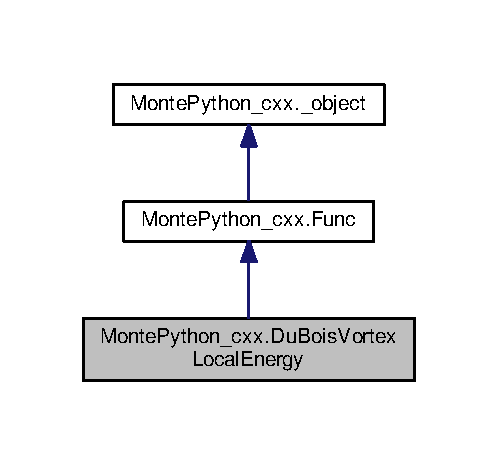
\includegraphics[width=239pt]{classMontePython__cxx_1_1DuBoisVortexLocalEnergy__inherit__graph}
\end{center}
\end{figure}


Collaboration diagram for Monte\+Python\+\_\+cxx.\+Du\+Bois\+Vortex\+Local\+Energy\+:
\nopagebreak
\begin{figure}[H]
\begin{center}
\leavevmode
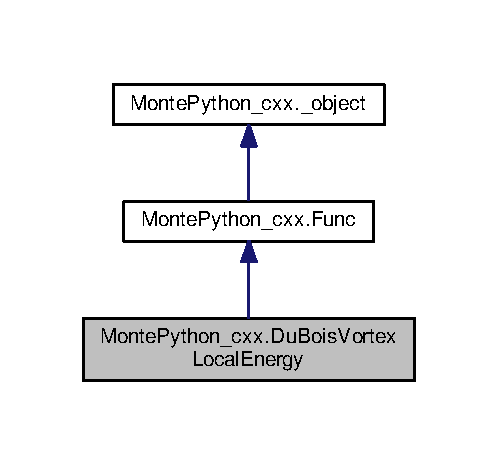
\includegraphics[width=239pt]{classMontePython__cxx_1_1DuBoisVortexLocalEnergy__coll__graph}
\end{center}
\end{figure}
\subsection*{Public Member Functions}
\begin{DoxyCompactItemize}
\item 
def \hyperlink{classMontePython__cxx_1_1DuBoisVortexLocalEnergy_a7f1e4b47cd09ee3e4a0267c3bd5d9c0f}{set\+Params} (self, args)
\item 
def \hyperlink{classMontePython__cxx_1_1DuBoisVortexLocalEnergy_a8498ea2cc21a3f75719898a94cd18f37}{value\+Pt} (self, args)
\item 
def \hyperlink{classMontePython__cxx_1_1DuBoisVortexLocalEnergy_abf60be54f40085a4fc12f017a0840798}{\+\_\+\+\_\+call\+\_\+\+\_\+} (self, args)
\item 
def \hyperlink{classMontePython__cxx_1_1DuBoisVortexLocalEnergy_ad82f61eb80d83a8b06230ddabe894c6a}{\+\_\+\+\_\+init\+\_\+\+\_\+} (self)
\end{DoxyCompactItemize}
\subsection*{Public Attributes}
\begin{DoxyCompactItemize}
\item 
\hypertarget{classMontePython__cxx_1_1DuBoisVortexLocalEnergy_a8e6644d2542ac629e9379b59c244d559}{}{\bfseries this}\label{classMontePython__cxx_1_1DuBoisVortexLocalEnergy_a8e6644d2542ac629e9379b59c244d559}

\end{DoxyCompactItemize}
\subsection*{Static Private Attributes}
\begin{DoxyCompactItemize}
\item 
\hypertarget{classMontePython__cxx_1_1DuBoisVortexLocalEnergy_a8098e80f915c4e629711bbd631f160f9}{}dictionary {\bfseries \+\_\+\+\_\+swig\+\_\+setmethods\+\_\+\+\_\+} = \{\}\label{classMontePython__cxx_1_1DuBoisVortexLocalEnergy_a8098e80f915c4e629711bbd631f160f9}

\item 
\hypertarget{classMontePython__cxx_1_1DuBoisVortexLocalEnergy_a837100dff9210e6793f46358a1d11242}{}tuple {\bfseries \+\_\+\+\_\+setattr\+\_\+\+\_\+} = lambdaself,name,value\+:\+\_\+swig\+\_\+setattr(self, \hyperlink{classMontePython__cxx_1_1DuBoisVortexLocalEnergy}{Du\+Bois\+Vortex\+Local\+Energy}, name, value)\label{classMontePython__cxx_1_1DuBoisVortexLocalEnergy_a837100dff9210e6793f46358a1d11242}

\item 
\hypertarget{classMontePython__cxx_1_1DuBoisVortexLocalEnergy_a510c0e9c23e19aacb0bf15ed79e9cbbf}{}dictionary {\bfseries \+\_\+\+\_\+swig\+\_\+getmethods\+\_\+\+\_\+} = \{\}\label{classMontePython__cxx_1_1DuBoisVortexLocalEnergy_a510c0e9c23e19aacb0bf15ed79e9cbbf}

\item 
\hypertarget{classMontePython__cxx_1_1DuBoisVortexLocalEnergy_a71f3c04894c1bb0c4f4c47be7fe19461}{}tuple {\bfseries \+\_\+\+\_\+getattr\+\_\+\+\_\+} = lambdaself,name\+:\+\_\+swig\+\_\+getattr(self, \hyperlink{classMontePython__cxx_1_1DuBoisVortexLocalEnergy}{Du\+Bois\+Vortex\+Local\+Energy}, name)\label{classMontePython__cxx_1_1DuBoisVortexLocalEnergy_a71f3c04894c1bb0c4f4c47be7fe19461}

\item 
\hypertarget{classMontePython__cxx_1_1DuBoisVortexLocalEnergy_a266322fc36cca6e54d9f7e53e3ef0a70}{}{\bfseries \+\_\+\+\_\+repr\+\_\+\+\_\+} = \+\_\+swig\+\_\+repr\label{classMontePython__cxx_1_1DuBoisVortexLocalEnergy_a266322fc36cca6e54d9f7e53e3ef0a70}

\item 
\hypertarget{classMontePython__cxx_1_1DuBoisVortexLocalEnergy_a5be62a2d2affb989d498d8bd9c91fa88}{}{\bfseries \+\_\+\+\_\+swig\+\_\+destroy\+\_\+\+\_\+} = \+\_\+\+Monte\+Python\+\_\+cxx.\+delete\+\_\+\+Du\+Bois\+Vortex\+Local\+Energy\label{classMontePython__cxx_1_1DuBoisVortexLocalEnergy_a5be62a2d2affb989d498d8bd9c91fa88}

\end{DoxyCompactItemize}


\subsection{Detailed Description}
\begin{DoxyVerb}Proxy of C++ DuBoisVortexLocalEnergy class\end{DoxyVerb}
 

\subsection{Constructor \& Destructor Documentation}
\hypertarget{classMontePython__cxx_1_1DuBoisVortexLocalEnergy_ad82f61eb80d83a8b06230ddabe894c6a}{}\index{Monte\+Python\+\_\+cxx\+::\+Du\+Bois\+Vortex\+Local\+Energy@{Monte\+Python\+\_\+cxx\+::\+Du\+Bois\+Vortex\+Local\+Energy}!\+\_\+\+\_\+init\+\_\+\+\_\+@{\+\_\+\+\_\+init\+\_\+\+\_\+}}
\index{\+\_\+\+\_\+init\+\_\+\+\_\+@{\+\_\+\+\_\+init\+\_\+\+\_\+}!Monte\+Python\+\_\+cxx\+::\+Du\+Bois\+Vortex\+Local\+Energy@{Monte\+Python\+\_\+cxx\+::\+Du\+Bois\+Vortex\+Local\+Energy}}
\subsubsection[{\+\_\+\+\_\+init\+\_\+\+\_\+}]{\setlength{\rightskip}{0pt plus 5cm}def Monte\+Python\+\_\+cxx.\+Du\+Bois\+Vortex\+Local\+Energy.\+\_\+\+\_\+init\+\_\+\+\_\+ (
\begin{DoxyParamCaption}
\item[{}]{self}
\end{DoxyParamCaption}
)}\label{classMontePython__cxx_1_1DuBoisVortexLocalEnergy_ad82f61eb80d83a8b06230ddabe894c6a}
\begin{DoxyVerb}__init__(DuBoisVortexLocalEnergy self) -> DuBoisVortexLocalEnergy\end{DoxyVerb}
 

\subsection{Member Function Documentation}
\hypertarget{classMontePython__cxx_1_1DuBoisVortexLocalEnergy_abf60be54f40085a4fc12f017a0840798}{}\index{Monte\+Python\+\_\+cxx\+::\+Du\+Bois\+Vortex\+Local\+Energy@{Monte\+Python\+\_\+cxx\+::\+Du\+Bois\+Vortex\+Local\+Energy}!\+\_\+\+\_\+call\+\_\+\+\_\+@{\+\_\+\+\_\+call\+\_\+\+\_\+}}
\index{\+\_\+\+\_\+call\+\_\+\+\_\+@{\+\_\+\+\_\+call\+\_\+\+\_\+}!Monte\+Python\+\_\+cxx\+::\+Du\+Bois\+Vortex\+Local\+Energy@{Monte\+Python\+\_\+cxx\+::\+Du\+Bois\+Vortex\+Local\+Energy}}
\subsubsection[{\+\_\+\+\_\+call\+\_\+\+\_\+}]{\setlength{\rightskip}{0pt plus 5cm}def Monte\+Python\+\_\+cxx.\+Du\+Bois\+Vortex\+Local\+Energy.\+\_\+\+\_\+call\+\_\+\+\_\+ (
\begin{DoxyParamCaption}
\item[{}]{self, }
\item[{}]{args}
\end{DoxyParamCaption}
)}\label{classMontePython__cxx_1_1DuBoisVortexLocalEnergy_abf60be54f40085a4fc12f017a0840798}
\begin{DoxyVerb}__call__(DuBoisVortexLocalEnergy self, QickArray & pos) -> double\end{DoxyVerb}
 \hypertarget{classMontePython__cxx_1_1DuBoisVortexLocalEnergy_a7f1e4b47cd09ee3e4a0267c3bd5d9c0f}{}\index{Monte\+Python\+\_\+cxx\+::\+Du\+Bois\+Vortex\+Local\+Energy@{Monte\+Python\+\_\+cxx\+::\+Du\+Bois\+Vortex\+Local\+Energy}!set\+Params@{set\+Params}}
\index{set\+Params@{set\+Params}!Monte\+Python\+\_\+cxx\+::\+Du\+Bois\+Vortex\+Local\+Energy@{Monte\+Python\+\_\+cxx\+::\+Du\+Bois\+Vortex\+Local\+Energy}}
\subsubsection[{set\+Params}]{\setlength{\rightskip}{0pt plus 5cm}def Monte\+Python\+\_\+cxx.\+Du\+Bois\+Vortex\+Local\+Energy.\+set\+Params (
\begin{DoxyParamCaption}
\item[{}]{self, }
\item[{}]{args}
\end{DoxyParamCaption}
)}\label{classMontePython__cxx_1_1DuBoisVortexLocalEnergy_a7f1e4b47cd09ee3e4a0267c3bd5d9c0f}
\begin{DoxyVerb}setParams(DuBoisVortexLocalEnergy self, QickArray & params_)\end{DoxyVerb}
 \hypertarget{classMontePython__cxx_1_1DuBoisVortexLocalEnergy_a8498ea2cc21a3f75719898a94cd18f37}{}\index{Monte\+Python\+\_\+cxx\+::\+Du\+Bois\+Vortex\+Local\+Energy@{Monte\+Python\+\_\+cxx\+::\+Du\+Bois\+Vortex\+Local\+Energy}!value\+Pt@{value\+Pt}}
\index{value\+Pt@{value\+Pt}!Monte\+Python\+\_\+cxx\+::\+Du\+Bois\+Vortex\+Local\+Energy@{Monte\+Python\+\_\+cxx\+::\+Du\+Bois\+Vortex\+Local\+Energy}}
\subsubsection[{value\+Pt}]{\setlength{\rightskip}{0pt plus 5cm}def Monte\+Python\+\_\+cxx.\+Du\+Bois\+Vortex\+Local\+Energy.\+value\+Pt (
\begin{DoxyParamCaption}
\item[{}]{self, }
\item[{}]{args}
\end{DoxyParamCaption}
)}\label{classMontePython__cxx_1_1DuBoisVortexLocalEnergy_a8498ea2cc21a3f75719898a94cd18f37}
\begin{DoxyVerb}valuePt(DuBoisVortexLocalEnergy self, QickArray & pos) -> double
valuePt(DuBoisVortexLocalEnergy self, QickArray & pos, int dummy) -> double
\end{DoxyVerb}
 

The documentation for this class was generated from the following file\+:\begin{DoxyCompactItemize}
\item 
Monte\+Python\+\_\+cxx.\+py\end{DoxyCompactItemize}

\hypertarget{classMontePython__cxx_1_1DuBoisVortexPotentialEnergy}{}\section{Monte\+Python\+\_\+cxx.\+Du\+Bois\+Vortex\+Potential\+Energy Class Reference}
\label{classMontePython__cxx_1_1DuBoisVortexPotentialEnergy}\index{Monte\+Python\+\_\+cxx.\+Du\+Bois\+Vortex\+Potential\+Energy@{Monte\+Python\+\_\+cxx.\+Du\+Bois\+Vortex\+Potential\+Energy}}


Inheritance diagram for Monte\+Python\+\_\+cxx.\+Du\+Bois\+Vortex\+Potential\+Energy\+:
\nopagebreak
\begin{figure}[H]
\begin{center}
\leavevmode
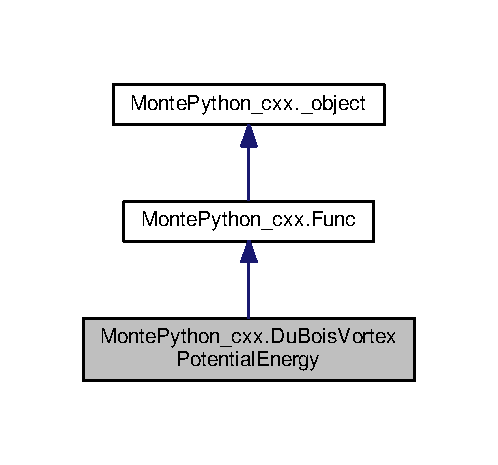
\includegraphics[width=239pt]{classMontePython__cxx_1_1DuBoisVortexPotentialEnergy__inherit__graph}
\end{center}
\end{figure}


Collaboration diagram for Monte\+Python\+\_\+cxx.\+Du\+Bois\+Vortex\+Potential\+Energy\+:
\nopagebreak
\begin{figure}[H]
\begin{center}
\leavevmode
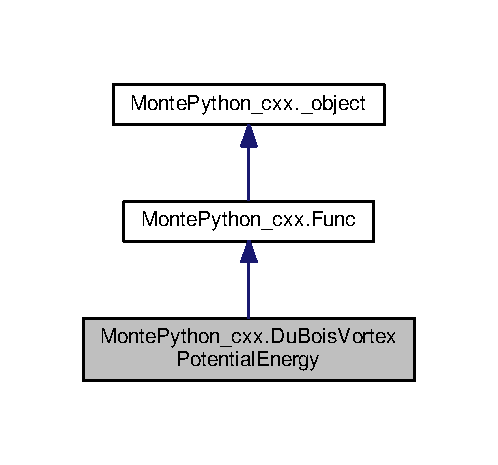
\includegraphics[width=239pt]{classMontePython__cxx_1_1DuBoisVortexPotentialEnergy__coll__graph}
\end{center}
\end{figure}
\subsection*{Public Member Functions}
\begin{DoxyCompactItemize}
\item 
def \hyperlink{classMontePython__cxx_1_1DuBoisVortexPotentialEnergy_a9e864e23293e662266f7b748a023b6dc}{set\+Params} (self, args)
\item 
def \hyperlink{classMontePython__cxx_1_1DuBoisVortexPotentialEnergy_acc4d803fdb2430eec51bd19cb17ded1e}{value\+Pt} (self, args)
\item 
def \hyperlink{classMontePython__cxx_1_1DuBoisVortexPotentialEnergy_aa99e01acccd564c434fc5003ee884964}{\+\_\+\+\_\+call\+\_\+\+\_\+} (self, args)
\item 
def \hyperlink{classMontePython__cxx_1_1DuBoisVortexPotentialEnergy_ae96f2dd2a8b52ce915334eabfdce4758}{\+\_\+\+\_\+init\+\_\+\+\_\+} (self)
\end{DoxyCompactItemize}
\subsection*{Public Attributes}
\begin{DoxyCompactItemize}
\item 
\hypertarget{classMontePython__cxx_1_1DuBoisVortexPotentialEnergy_aa3b2d56c347a6c529c6127d0c94872b2}{}{\bfseries this}\label{classMontePython__cxx_1_1DuBoisVortexPotentialEnergy_aa3b2d56c347a6c529c6127d0c94872b2}

\end{DoxyCompactItemize}
\subsection*{Static Private Attributes}
\begin{DoxyCompactItemize}
\item 
\hypertarget{classMontePython__cxx_1_1DuBoisVortexPotentialEnergy_ad7d505785f4e3b3955bd01d6cebe19a2}{}dictionary {\bfseries \+\_\+\+\_\+swig\+\_\+setmethods\+\_\+\+\_\+} = \{\}\label{classMontePython__cxx_1_1DuBoisVortexPotentialEnergy_ad7d505785f4e3b3955bd01d6cebe19a2}

\item 
\hypertarget{classMontePython__cxx_1_1DuBoisVortexPotentialEnergy_aaf882c179de55b9d16aecf4c48099204}{}tuple {\bfseries \+\_\+\+\_\+setattr\+\_\+\+\_\+} = lambdaself,name,value\+:\+\_\+swig\+\_\+setattr(self, \hyperlink{classMontePython__cxx_1_1DuBoisVortexPotentialEnergy}{Du\+Bois\+Vortex\+Potential\+Energy}, name, value)\label{classMontePython__cxx_1_1DuBoisVortexPotentialEnergy_aaf882c179de55b9d16aecf4c48099204}

\item 
\hypertarget{classMontePython__cxx_1_1DuBoisVortexPotentialEnergy_ae02ea0c6be3d7f1b2d1b78c02641dd68}{}dictionary {\bfseries \+\_\+\+\_\+swig\+\_\+getmethods\+\_\+\+\_\+} = \{\}\label{classMontePython__cxx_1_1DuBoisVortexPotentialEnergy_ae02ea0c6be3d7f1b2d1b78c02641dd68}

\item 
\hypertarget{classMontePython__cxx_1_1DuBoisVortexPotentialEnergy_aa193df97e843c1273b77eea21857e080}{}tuple {\bfseries \+\_\+\+\_\+getattr\+\_\+\+\_\+} = lambdaself,name\+:\+\_\+swig\+\_\+getattr(self, \hyperlink{classMontePython__cxx_1_1DuBoisVortexPotentialEnergy}{Du\+Bois\+Vortex\+Potential\+Energy}, name)\label{classMontePython__cxx_1_1DuBoisVortexPotentialEnergy_aa193df97e843c1273b77eea21857e080}

\item 
\hypertarget{classMontePython__cxx_1_1DuBoisVortexPotentialEnergy_a71b13419fb64ca1d96b3e42b3bc0ee72}{}{\bfseries \+\_\+\+\_\+repr\+\_\+\+\_\+} = \+\_\+swig\+\_\+repr\label{classMontePython__cxx_1_1DuBoisVortexPotentialEnergy_a71b13419fb64ca1d96b3e42b3bc0ee72}

\item 
\hypertarget{classMontePython__cxx_1_1DuBoisVortexPotentialEnergy_a394c1ee60ee4c0f2c86cab93387d0b4b}{}{\bfseries \+\_\+\+\_\+swig\+\_\+destroy\+\_\+\+\_\+} = \+\_\+\+Monte\+Python\+\_\+cxx.\+delete\+\_\+\+Du\+Bois\+Vortex\+Potential\+Energy\label{classMontePython__cxx_1_1DuBoisVortexPotentialEnergy_a394c1ee60ee4c0f2c86cab93387d0b4b}

\end{DoxyCompactItemize}


\subsection{Detailed Description}
\begin{DoxyVerb}Proxy of C++ DuBoisVortexPotentialEnergy class\end{DoxyVerb}
 

\subsection{Constructor \& Destructor Documentation}
\hypertarget{classMontePython__cxx_1_1DuBoisVortexPotentialEnergy_ae96f2dd2a8b52ce915334eabfdce4758}{}\index{Monte\+Python\+\_\+cxx\+::\+Du\+Bois\+Vortex\+Potential\+Energy@{Monte\+Python\+\_\+cxx\+::\+Du\+Bois\+Vortex\+Potential\+Energy}!\+\_\+\+\_\+init\+\_\+\+\_\+@{\+\_\+\+\_\+init\+\_\+\+\_\+}}
\index{\+\_\+\+\_\+init\+\_\+\+\_\+@{\+\_\+\+\_\+init\+\_\+\+\_\+}!Monte\+Python\+\_\+cxx\+::\+Du\+Bois\+Vortex\+Potential\+Energy@{Monte\+Python\+\_\+cxx\+::\+Du\+Bois\+Vortex\+Potential\+Energy}}
\subsubsection[{\+\_\+\+\_\+init\+\_\+\+\_\+}]{\setlength{\rightskip}{0pt plus 5cm}def Monte\+Python\+\_\+cxx.\+Du\+Bois\+Vortex\+Potential\+Energy.\+\_\+\+\_\+init\+\_\+\+\_\+ (
\begin{DoxyParamCaption}
\item[{}]{self}
\end{DoxyParamCaption}
)}\label{classMontePython__cxx_1_1DuBoisVortexPotentialEnergy_ae96f2dd2a8b52ce915334eabfdce4758}
\begin{DoxyVerb}__init__(DuBoisVortexPotentialEnergy self) -> DuBoisVortexPotentialEnergy\end{DoxyVerb}
 

\subsection{Member Function Documentation}
\hypertarget{classMontePython__cxx_1_1DuBoisVortexPotentialEnergy_aa99e01acccd564c434fc5003ee884964}{}\index{Monte\+Python\+\_\+cxx\+::\+Du\+Bois\+Vortex\+Potential\+Energy@{Monte\+Python\+\_\+cxx\+::\+Du\+Bois\+Vortex\+Potential\+Energy}!\+\_\+\+\_\+call\+\_\+\+\_\+@{\+\_\+\+\_\+call\+\_\+\+\_\+}}
\index{\+\_\+\+\_\+call\+\_\+\+\_\+@{\+\_\+\+\_\+call\+\_\+\+\_\+}!Monte\+Python\+\_\+cxx\+::\+Du\+Bois\+Vortex\+Potential\+Energy@{Monte\+Python\+\_\+cxx\+::\+Du\+Bois\+Vortex\+Potential\+Energy}}
\subsubsection[{\+\_\+\+\_\+call\+\_\+\+\_\+}]{\setlength{\rightskip}{0pt plus 5cm}def Monte\+Python\+\_\+cxx.\+Du\+Bois\+Vortex\+Potential\+Energy.\+\_\+\+\_\+call\+\_\+\+\_\+ (
\begin{DoxyParamCaption}
\item[{}]{self, }
\item[{}]{args}
\end{DoxyParamCaption}
)}\label{classMontePython__cxx_1_1DuBoisVortexPotentialEnergy_aa99e01acccd564c434fc5003ee884964}
\begin{DoxyVerb}__call__(DuBoisVortexPotentialEnergy self, QickArray & pos) -> double\end{DoxyVerb}
 \hypertarget{classMontePython__cxx_1_1DuBoisVortexPotentialEnergy_a9e864e23293e662266f7b748a023b6dc}{}\index{Monte\+Python\+\_\+cxx\+::\+Du\+Bois\+Vortex\+Potential\+Energy@{Monte\+Python\+\_\+cxx\+::\+Du\+Bois\+Vortex\+Potential\+Energy}!set\+Params@{set\+Params}}
\index{set\+Params@{set\+Params}!Monte\+Python\+\_\+cxx\+::\+Du\+Bois\+Vortex\+Potential\+Energy@{Monte\+Python\+\_\+cxx\+::\+Du\+Bois\+Vortex\+Potential\+Energy}}
\subsubsection[{set\+Params}]{\setlength{\rightskip}{0pt plus 5cm}def Monte\+Python\+\_\+cxx.\+Du\+Bois\+Vortex\+Potential\+Energy.\+set\+Params (
\begin{DoxyParamCaption}
\item[{}]{self, }
\item[{}]{args}
\end{DoxyParamCaption}
)}\label{classMontePython__cxx_1_1DuBoisVortexPotentialEnergy_a9e864e23293e662266f7b748a023b6dc}
\begin{DoxyVerb}setParams(DuBoisVortexPotentialEnergy self, QickArray & params_)\end{DoxyVerb}
 \hypertarget{classMontePython__cxx_1_1DuBoisVortexPotentialEnergy_acc4d803fdb2430eec51bd19cb17ded1e}{}\index{Monte\+Python\+\_\+cxx\+::\+Du\+Bois\+Vortex\+Potential\+Energy@{Monte\+Python\+\_\+cxx\+::\+Du\+Bois\+Vortex\+Potential\+Energy}!value\+Pt@{value\+Pt}}
\index{value\+Pt@{value\+Pt}!Monte\+Python\+\_\+cxx\+::\+Du\+Bois\+Vortex\+Potential\+Energy@{Monte\+Python\+\_\+cxx\+::\+Du\+Bois\+Vortex\+Potential\+Energy}}
\subsubsection[{value\+Pt}]{\setlength{\rightskip}{0pt plus 5cm}def Monte\+Python\+\_\+cxx.\+Du\+Bois\+Vortex\+Potential\+Energy.\+value\+Pt (
\begin{DoxyParamCaption}
\item[{}]{self, }
\item[{}]{args}
\end{DoxyParamCaption}
)}\label{classMontePython__cxx_1_1DuBoisVortexPotentialEnergy_acc4d803fdb2430eec51bd19cb17ded1e}
\begin{DoxyVerb}valuePt(DuBoisVortexPotentialEnergy self, QickArray & pos) -> double\end{DoxyVerb}
 

The documentation for this class was generated from the following file\+:\begin{DoxyCompactItemize}
\item 
Monte\+Python\+\_\+cxx.\+py\end{DoxyCompactItemize}

\hypertarget{classMontePython__cxx_1_1DuBoisVortexQForce}{}\section{Monte\+Python\+\_\+cxx.\+Du\+Bois\+Vortex\+Q\+Force Class Reference}
\label{classMontePython__cxx_1_1DuBoisVortexQForce}\index{Monte\+Python\+\_\+cxx.\+Du\+Bois\+Vortex\+Q\+Force@{Monte\+Python\+\_\+cxx.\+Du\+Bois\+Vortex\+Q\+Force}}


Inheritance diagram for Monte\+Python\+\_\+cxx.\+Du\+Bois\+Vortex\+Q\+Force\+:
\nopagebreak
\begin{figure}[H]
\begin{center}
\leavevmode
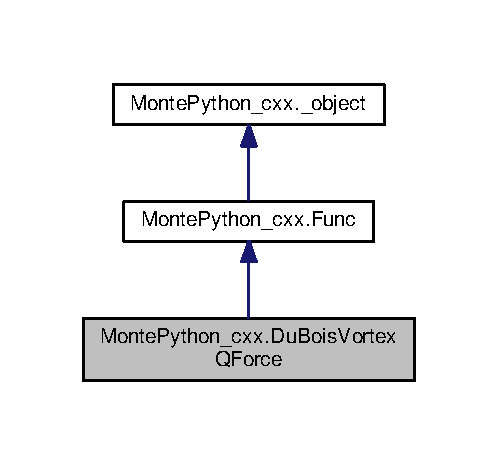
\includegraphics[width=239pt]{classMontePython__cxx_1_1DuBoisVortexQForce__inherit__graph}
\end{center}
\end{figure}


Collaboration diagram for Monte\+Python\+\_\+cxx.\+Du\+Bois\+Vortex\+Q\+Force\+:
\nopagebreak
\begin{figure}[H]
\begin{center}
\leavevmode
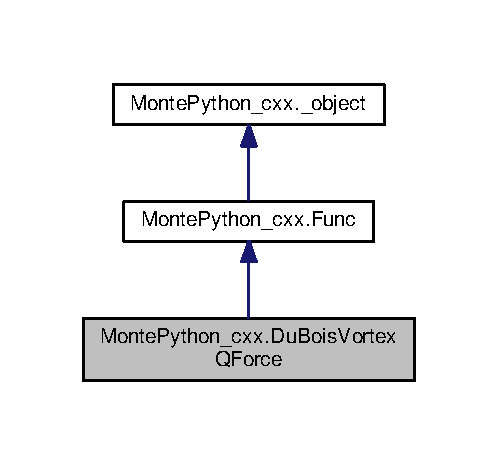
\includegraphics[width=239pt]{classMontePython__cxx_1_1DuBoisVortexQForce__coll__graph}
\end{center}
\end{figure}
\subsection*{Public Member Functions}
\begin{DoxyCompactItemize}
\item 
def \hyperlink{classMontePython__cxx_1_1DuBoisVortexQForce_aeb1c00839a5a09dbdf960e0185d8da22}{set\+Params} (self, args)
\item 
def \hyperlink{classMontePython__cxx_1_1DuBoisVortexQForce_a148ac1a5e9b3ff24c712de9f54d446e3}{value\+Pt} (self, args)
\item 
def \hyperlink{classMontePython__cxx_1_1DuBoisVortexQForce_a96d4afd698fb8f45a745e1f1a9c7d7f0}{\+\_\+\+\_\+call\+\_\+\+\_\+} (self, args)
\item 
def \hyperlink{classMontePython__cxx_1_1DuBoisVortexQForce_ac45faf207de6abd9be9702d8eaab6f04}{\+\_\+\+\_\+init\+\_\+\+\_\+} (self)
\end{DoxyCompactItemize}
\subsection*{Public Attributes}
\begin{DoxyCompactItemize}
\item 
\hypertarget{classMontePython__cxx_1_1DuBoisVortexQForce_a6790f6c4b729fabd04e6d6b90b3b0496}{}{\bfseries this}\label{classMontePython__cxx_1_1DuBoisVortexQForce_a6790f6c4b729fabd04e6d6b90b3b0496}

\end{DoxyCompactItemize}
\subsection*{Static Private Attributes}
\begin{DoxyCompactItemize}
\item 
\hypertarget{classMontePython__cxx_1_1DuBoisVortexQForce_ae7faa9f365cfa6fd9eddae86607a70f6}{}dictionary {\bfseries \+\_\+\+\_\+swig\+\_\+setmethods\+\_\+\+\_\+} = \{\}\label{classMontePython__cxx_1_1DuBoisVortexQForce_ae7faa9f365cfa6fd9eddae86607a70f6}

\item 
\hypertarget{classMontePython__cxx_1_1DuBoisVortexQForce_a838f4ae717c2932de827e303b27a1a18}{}tuple {\bfseries \+\_\+\+\_\+setattr\+\_\+\+\_\+} = lambdaself,name,value\+:\+\_\+swig\+\_\+setattr(self, \hyperlink{classMontePython__cxx_1_1DuBoisVortexQForce}{Du\+Bois\+Vortex\+Q\+Force}, name, value)\label{classMontePython__cxx_1_1DuBoisVortexQForce_a838f4ae717c2932de827e303b27a1a18}

\item 
\hypertarget{classMontePython__cxx_1_1DuBoisVortexQForce_a07d2c7eecf7fdddb58ed8ef3e2fe6a3d}{}dictionary {\bfseries \+\_\+\+\_\+swig\+\_\+getmethods\+\_\+\+\_\+} = \{\}\label{classMontePython__cxx_1_1DuBoisVortexQForce_a07d2c7eecf7fdddb58ed8ef3e2fe6a3d}

\item 
\hypertarget{classMontePython__cxx_1_1DuBoisVortexQForce_a7af95eb93c798a54077252e045d1a808}{}tuple {\bfseries \+\_\+\+\_\+getattr\+\_\+\+\_\+} = lambdaself,name\+:\+\_\+swig\+\_\+getattr(self, \hyperlink{classMontePython__cxx_1_1DuBoisVortexQForce}{Du\+Bois\+Vortex\+Q\+Force}, name)\label{classMontePython__cxx_1_1DuBoisVortexQForce_a7af95eb93c798a54077252e045d1a808}

\item 
\hypertarget{classMontePython__cxx_1_1DuBoisVortexQForce_ad3a2cf6785e0cb60f3a74c7beafe6a63}{}{\bfseries \+\_\+\+\_\+repr\+\_\+\+\_\+} = \+\_\+swig\+\_\+repr\label{classMontePython__cxx_1_1DuBoisVortexQForce_ad3a2cf6785e0cb60f3a74c7beafe6a63}

\item 
\hypertarget{classMontePython__cxx_1_1DuBoisVortexQForce_a4b5536845ffb35a2d5e5b1d1b5ec1925}{}{\bfseries \+\_\+\+\_\+swig\+\_\+destroy\+\_\+\+\_\+} = \+\_\+\+Monte\+Python\+\_\+cxx.\+delete\+\_\+\+Du\+Bois\+Vortex\+Q\+Force\label{classMontePython__cxx_1_1DuBoisVortexQForce_a4b5536845ffb35a2d5e5b1d1b5ec1925}

\end{DoxyCompactItemize}


\subsection{Detailed Description}
\begin{DoxyVerb}Proxy of C++ DuBoisVortexQForce class\end{DoxyVerb}
 

\subsection{Constructor \& Destructor Documentation}
\hypertarget{classMontePython__cxx_1_1DuBoisVortexQForce_ac45faf207de6abd9be9702d8eaab6f04}{}\index{Monte\+Python\+\_\+cxx\+::\+Du\+Bois\+Vortex\+Q\+Force@{Monte\+Python\+\_\+cxx\+::\+Du\+Bois\+Vortex\+Q\+Force}!\+\_\+\+\_\+init\+\_\+\+\_\+@{\+\_\+\+\_\+init\+\_\+\+\_\+}}
\index{\+\_\+\+\_\+init\+\_\+\+\_\+@{\+\_\+\+\_\+init\+\_\+\+\_\+}!Monte\+Python\+\_\+cxx\+::\+Du\+Bois\+Vortex\+Q\+Force@{Monte\+Python\+\_\+cxx\+::\+Du\+Bois\+Vortex\+Q\+Force}}
\subsubsection[{\+\_\+\+\_\+init\+\_\+\+\_\+}]{\setlength{\rightskip}{0pt plus 5cm}def Monte\+Python\+\_\+cxx.\+Du\+Bois\+Vortex\+Q\+Force.\+\_\+\+\_\+init\+\_\+\+\_\+ (
\begin{DoxyParamCaption}
\item[{}]{self}
\end{DoxyParamCaption}
)}\label{classMontePython__cxx_1_1DuBoisVortexQForce_ac45faf207de6abd9be9702d8eaab6f04}
\begin{DoxyVerb}__init__(DuBoisVortexQForce self) -> DuBoisVortexQForce\end{DoxyVerb}
 

\subsection{Member Function Documentation}
\hypertarget{classMontePython__cxx_1_1DuBoisVortexQForce_a96d4afd698fb8f45a745e1f1a9c7d7f0}{}\index{Monte\+Python\+\_\+cxx\+::\+Du\+Bois\+Vortex\+Q\+Force@{Monte\+Python\+\_\+cxx\+::\+Du\+Bois\+Vortex\+Q\+Force}!\+\_\+\+\_\+call\+\_\+\+\_\+@{\+\_\+\+\_\+call\+\_\+\+\_\+}}
\index{\+\_\+\+\_\+call\+\_\+\+\_\+@{\+\_\+\+\_\+call\+\_\+\+\_\+}!Monte\+Python\+\_\+cxx\+::\+Du\+Bois\+Vortex\+Q\+Force@{Monte\+Python\+\_\+cxx\+::\+Du\+Bois\+Vortex\+Q\+Force}}
\subsubsection[{\+\_\+\+\_\+call\+\_\+\+\_\+}]{\setlength{\rightskip}{0pt plus 5cm}def Monte\+Python\+\_\+cxx.\+Du\+Bois\+Vortex\+Q\+Force.\+\_\+\+\_\+call\+\_\+\+\_\+ (
\begin{DoxyParamCaption}
\item[{}]{self, }
\item[{}]{args}
\end{DoxyParamCaption}
)}\label{classMontePython__cxx_1_1DuBoisVortexQForce_a96d4afd698fb8f45a745e1f1a9c7d7f0}
\begin{DoxyVerb}__call__(DuBoisVortexQForce self, QickArray & pos, bool dummy) -> QickArray &\end{DoxyVerb}
 \hypertarget{classMontePython__cxx_1_1DuBoisVortexQForce_aeb1c00839a5a09dbdf960e0185d8da22}{}\index{Monte\+Python\+\_\+cxx\+::\+Du\+Bois\+Vortex\+Q\+Force@{Monte\+Python\+\_\+cxx\+::\+Du\+Bois\+Vortex\+Q\+Force}!set\+Params@{set\+Params}}
\index{set\+Params@{set\+Params}!Monte\+Python\+\_\+cxx\+::\+Du\+Bois\+Vortex\+Q\+Force@{Monte\+Python\+\_\+cxx\+::\+Du\+Bois\+Vortex\+Q\+Force}}
\subsubsection[{set\+Params}]{\setlength{\rightskip}{0pt plus 5cm}def Monte\+Python\+\_\+cxx.\+Du\+Bois\+Vortex\+Q\+Force.\+set\+Params (
\begin{DoxyParamCaption}
\item[{}]{self, }
\item[{}]{args}
\end{DoxyParamCaption}
)}\label{classMontePython__cxx_1_1DuBoisVortexQForce_aeb1c00839a5a09dbdf960e0185d8da22}
\begin{DoxyVerb}setParams(DuBoisVortexQForce self, QickArray & params_)\end{DoxyVerb}
 \hypertarget{classMontePython__cxx_1_1DuBoisVortexQForce_a148ac1a5e9b3ff24c712de9f54d446e3}{}\index{Monte\+Python\+\_\+cxx\+::\+Du\+Bois\+Vortex\+Q\+Force@{Monte\+Python\+\_\+cxx\+::\+Du\+Bois\+Vortex\+Q\+Force}!value\+Pt@{value\+Pt}}
\index{value\+Pt@{value\+Pt}!Monte\+Python\+\_\+cxx\+::\+Du\+Bois\+Vortex\+Q\+Force@{Monte\+Python\+\_\+cxx\+::\+Du\+Bois\+Vortex\+Q\+Force}}
\subsubsection[{value\+Pt}]{\setlength{\rightskip}{0pt plus 5cm}def Monte\+Python\+\_\+cxx.\+Du\+Bois\+Vortex\+Q\+Force.\+value\+Pt (
\begin{DoxyParamCaption}
\item[{}]{self, }
\item[{}]{args}
\end{DoxyParamCaption}
)}\label{classMontePython__cxx_1_1DuBoisVortexQForce_a148ac1a5e9b3ff24c712de9f54d446e3}
\begin{DoxyVerb}valuePt(DuBoisVortexQForce self, QickArray & pos, bool dummy) -> QickArray &\end{DoxyVerb}
 

The documentation for this class was generated from the following file\+:\begin{DoxyCompactItemize}
\item 
Monte\+Python\+\_\+cxx.\+py\end{DoxyCompactItemize}

\hypertarget{classMontePython__cxx_1_1DuBoisVortexWave}{}\section{Monte\+Python\+\_\+cxx.\+Du\+Bois\+Vortex\+Wave Class Reference}
\label{classMontePython__cxx_1_1DuBoisVortexWave}\index{Monte\+Python\+\_\+cxx.\+Du\+Bois\+Vortex\+Wave@{Monte\+Python\+\_\+cxx.\+Du\+Bois\+Vortex\+Wave}}


Inheritance diagram for Monte\+Python\+\_\+cxx.\+Du\+Bois\+Vortex\+Wave\+:
\nopagebreak
\begin{figure}[H]
\begin{center}
\leavevmode
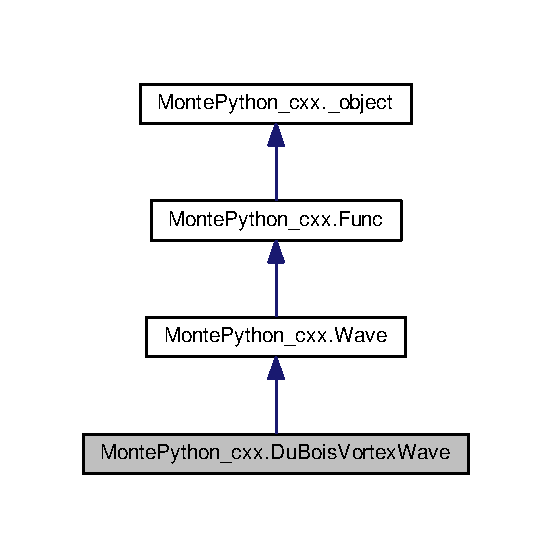
\includegraphics[width=265pt]{classMontePython__cxx_1_1DuBoisVortexWave__inherit__graph}
\end{center}
\end{figure}


Collaboration diagram for Monte\+Python\+\_\+cxx.\+Du\+Bois\+Vortex\+Wave\+:
\nopagebreak
\begin{figure}[H]
\begin{center}
\leavevmode
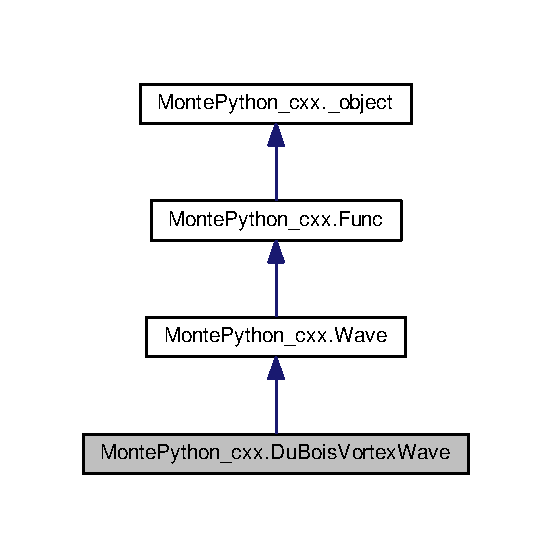
\includegraphics[width=265pt]{classMontePython__cxx_1_1DuBoisVortexWave__coll__graph}
\end{center}
\end{figure}
\subsection*{Public Member Functions}
\begin{DoxyCompactItemize}
\item 
def \hyperlink{classMontePython__cxx_1_1DuBoisVortexWave_ace69a9a9446930b58685c2857676149a}{set\+Params} (self, args)
\item 
def \hyperlink{classMontePython__cxx_1_1DuBoisVortexWave_a2c2b35f9369210fa49d9c08e410b61b1}{value\+Pt} (self, args)
\item 
def \hyperlink{classMontePython__cxx_1_1DuBoisVortexWave_aeeec49f1d8b8a9dc18a8acca9f1bdfe9}{\+\_\+\+\_\+call\+\_\+\+\_\+} (self, args)
\item 
def \hyperlink{classMontePython__cxx_1_1DuBoisVortexWave_a859ea18b245d99474fa5fae54cf62954}{\+\_\+\+\_\+init\+\_\+\+\_\+} (self)
\end{DoxyCompactItemize}
\subsection*{Public Attributes}
\begin{DoxyCompactItemize}
\item 
\hypertarget{classMontePython__cxx_1_1DuBoisVortexWave_a56fe011bdc8b78ce09b17955b376fe12}{}{\bfseries this}\label{classMontePython__cxx_1_1DuBoisVortexWave_a56fe011bdc8b78ce09b17955b376fe12}

\end{DoxyCompactItemize}
\subsection*{Static Private Attributes}
\begin{DoxyCompactItemize}
\item 
\hypertarget{classMontePython__cxx_1_1DuBoisVortexWave_a6c62fd054ed29f57836a81859e349e59}{}dictionary {\bfseries \+\_\+\+\_\+swig\+\_\+setmethods\+\_\+\+\_\+} = \{\}\label{classMontePython__cxx_1_1DuBoisVortexWave_a6c62fd054ed29f57836a81859e349e59}

\item 
\hypertarget{classMontePython__cxx_1_1DuBoisVortexWave_a523f89ac79561d337d9a6c94de2e6d5c}{}tuple {\bfseries \+\_\+\+\_\+setattr\+\_\+\+\_\+} = lambdaself,name,value\+:\+\_\+swig\+\_\+setattr(self, \hyperlink{classMontePython__cxx_1_1DuBoisVortexWave}{Du\+Bois\+Vortex\+Wave}, name, value)\label{classMontePython__cxx_1_1DuBoisVortexWave_a523f89ac79561d337d9a6c94de2e6d5c}

\item 
\hypertarget{classMontePython__cxx_1_1DuBoisVortexWave_aee927f6b24ebe352c67c2f3c5347c16c}{}dictionary {\bfseries \+\_\+\+\_\+swig\+\_\+getmethods\+\_\+\+\_\+} = \{\}\label{classMontePython__cxx_1_1DuBoisVortexWave_aee927f6b24ebe352c67c2f3c5347c16c}

\item 
\hypertarget{classMontePython__cxx_1_1DuBoisVortexWave_a385469e58fb4683e8f75ff3c5a1a4537}{}tuple {\bfseries \+\_\+\+\_\+getattr\+\_\+\+\_\+} = lambdaself,name\+:\+\_\+swig\+\_\+getattr(self, \hyperlink{classMontePython__cxx_1_1DuBoisVortexWave}{Du\+Bois\+Vortex\+Wave}, name)\label{classMontePython__cxx_1_1DuBoisVortexWave_a385469e58fb4683e8f75ff3c5a1a4537}

\item 
\hypertarget{classMontePython__cxx_1_1DuBoisVortexWave_a16c8b8f4e8d7f8cdbd9931a7593154dc}{}{\bfseries \+\_\+\+\_\+repr\+\_\+\+\_\+} = \+\_\+swig\+\_\+repr\label{classMontePython__cxx_1_1DuBoisVortexWave_a16c8b8f4e8d7f8cdbd9931a7593154dc}

\item 
\hypertarget{classMontePython__cxx_1_1DuBoisVortexWave_ae8f11b9ac8369695c12053a708075d31}{}{\bfseries \+\_\+\+\_\+swig\+\_\+destroy\+\_\+\+\_\+} = \+\_\+\+Monte\+Python\+\_\+cxx.\+delete\+\_\+\+Du\+Bois\+Vortex\+Wave\label{classMontePython__cxx_1_1DuBoisVortexWave_ae8f11b9ac8369695c12053a708075d31}

\end{DoxyCompactItemize}


\subsection{Detailed Description}
\begin{DoxyVerb}Proxy of C++ DuBoisVortexWave class\end{DoxyVerb}
 

\subsection{Constructor \& Destructor Documentation}
\hypertarget{classMontePython__cxx_1_1DuBoisVortexWave_a859ea18b245d99474fa5fae54cf62954}{}\index{Monte\+Python\+\_\+cxx\+::\+Du\+Bois\+Vortex\+Wave@{Monte\+Python\+\_\+cxx\+::\+Du\+Bois\+Vortex\+Wave}!\+\_\+\+\_\+init\+\_\+\+\_\+@{\+\_\+\+\_\+init\+\_\+\+\_\+}}
\index{\+\_\+\+\_\+init\+\_\+\+\_\+@{\+\_\+\+\_\+init\+\_\+\+\_\+}!Monte\+Python\+\_\+cxx\+::\+Du\+Bois\+Vortex\+Wave@{Monte\+Python\+\_\+cxx\+::\+Du\+Bois\+Vortex\+Wave}}
\subsubsection[{\+\_\+\+\_\+init\+\_\+\+\_\+}]{\setlength{\rightskip}{0pt plus 5cm}def Monte\+Python\+\_\+cxx.\+Du\+Bois\+Vortex\+Wave.\+\_\+\+\_\+init\+\_\+\+\_\+ (
\begin{DoxyParamCaption}
\item[{}]{self}
\end{DoxyParamCaption}
)}\label{classMontePython__cxx_1_1DuBoisVortexWave_a859ea18b245d99474fa5fae54cf62954}
\begin{DoxyVerb}__init__(DuBoisVortexWave self) -> DuBoisVortexWave\end{DoxyVerb}
 

\subsection{Member Function Documentation}
\hypertarget{classMontePython__cxx_1_1DuBoisVortexWave_aeeec49f1d8b8a9dc18a8acca9f1bdfe9}{}\index{Monte\+Python\+\_\+cxx\+::\+Du\+Bois\+Vortex\+Wave@{Monte\+Python\+\_\+cxx\+::\+Du\+Bois\+Vortex\+Wave}!\+\_\+\+\_\+call\+\_\+\+\_\+@{\+\_\+\+\_\+call\+\_\+\+\_\+}}
\index{\+\_\+\+\_\+call\+\_\+\+\_\+@{\+\_\+\+\_\+call\+\_\+\+\_\+}!Monte\+Python\+\_\+cxx\+::\+Du\+Bois\+Vortex\+Wave@{Monte\+Python\+\_\+cxx\+::\+Du\+Bois\+Vortex\+Wave}}
\subsubsection[{\+\_\+\+\_\+call\+\_\+\+\_\+}]{\setlength{\rightskip}{0pt plus 5cm}def Monte\+Python\+\_\+cxx.\+Du\+Bois\+Vortex\+Wave.\+\_\+\+\_\+call\+\_\+\+\_\+ (
\begin{DoxyParamCaption}
\item[{}]{self, }
\item[{}]{args}
\end{DoxyParamCaption}
)}\label{classMontePython__cxx_1_1DuBoisVortexWave_aeeec49f1d8b8a9dc18a8acca9f1bdfe9}
\begin{DoxyVerb}__call__(DuBoisVortexWave self, QickArray & pos) -> double\end{DoxyVerb}
 \hypertarget{classMontePython__cxx_1_1DuBoisVortexWave_ace69a9a9446930b58685c2857676149a}{}\index{Monte\+Python\+\_\+cxx\+::\+Du\+Bois\+Vortex\+Wave@{Monte\+Python\+\_\+cxx\+::\+Du\+Bois\+Vortex\+Wave}!set\+Params@{set\+Params}}
\index{set\+Params@{set\+Params}!Monte\+Python\+\_\+cxx\+::\+Du\+Bois\+Vortex\+Wave@{Monte\+Python\+\_\+cxx\+::\+Du\+Bois\+Vortex\+Wave}}
\subsubsection[{set\+Params}]{\setlength{\rightskip}{0pt plus 5cm}def Monte\+Python\+\_\+cxx.\+Du\+Bois\+Vortex\+Wave.\+set\+Params (
\begin{DoxyParamCaption}
\item[{}]{self, }
\item[{}]{args}
\end{DoxyParamCaption}
)}\label{classMontePython__cxx_1_1DuBoisVortexWave_ace69a9a9446930b58685c2857676149a}
\begin{DoxyVerb}setParams(DuBoisVortexWave self, QickArray & params_)\end{DoxyVerb}
 \hypertarget{classMontePython__cxx_1_1DuBoisVortexWave_a2c2b35f9369210fa49d9c08e410b61b1}{}\index{Monte\+Python\+\_\+cxx\+::\+Du\+Bois\+Vortex\+Wave@{Monte\+Python\+\_\+cxx\+::\+Du\+Bois\+Vortex\+Wave}!value\+Pt@{value\+Pt}}
\index{value\+Pt@{value\+Pt}!Monte\+Python\+\_\+cxx\+::\+Du\+Bois\+Vortex\+Wave@{Monte\+Python\+\_\+cxx\+::\+Du\+Bois\+Vortex\+Wave}}
\subsubsection[{value\+Pt}]{\setlength{\rightskip}{0pt plus 5cm}def Monte\+Python\+\_\+cxx.\+Du\+Bois\+Vortex\+Wave.\+value\+Pt (
\begin{DoxyParamCaption}
\item[{}]{self, }
\item[{}]{args}
\end{DoxyParamCaption}
)}\label{classMontePython__cxx_1_1DuBoisVortexWave_a2c2b35f9369210fa49d9c08e410b61b1}
\begin{DoxyVerb}valuePt(DuBoisVortexWave self, QickArray & pos) -> double\end{DoxyVerb}
 

The documentation for this class was generated from the following file\+:\begin{DoxyCompactItemize}
\item 
Monte\+Python\+\_\+cxx.\+py\end{DoxyCompactItemize}

\hypertarget{classMontePython__cxx_1_1DuBoisVortexWaveAll}{}\section{Monte\+Python\+\_\+cxx.\+Du\+Bois\+Vortex\+Wave\+All Class Reference}
\label{classMontePython__cxx_1_1DuBoisVortexWaveAll}\index{Monte\+Python\+\_\+cxx.\+Du\+Bois\+Vortex\+Wave\+All@{Monte\+Python\+\_\+cxx.\+Du\+Bois\+Vortex\+Wave\+All}}


Inheritance diagram for Monte\+Python\+\_\+cxx.\+Du\+Bois\+Vortex\+Wave\+All\+:
\nopagebreak
\begin{figure}[H]
\begin{center}
\leavevmode
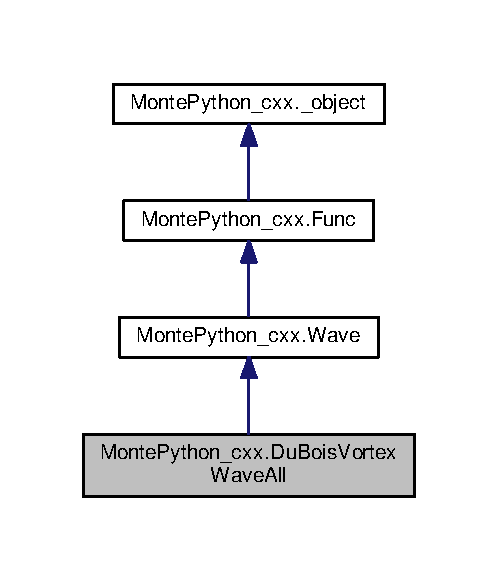
\includegraphics[width=239pt]{classMontePython__cxx_1_1DuBoisVortexWaveAll__inherit__graph}
\end{center}
\end{figure}


Collaboration diagram for Monte\+Python\+\_\+cxx.\+Du\+Bois\+Vortex\+Wave\+All\+:
\nopagebreak
\begin{figure}[H]
\begin{center}
\leavevmode
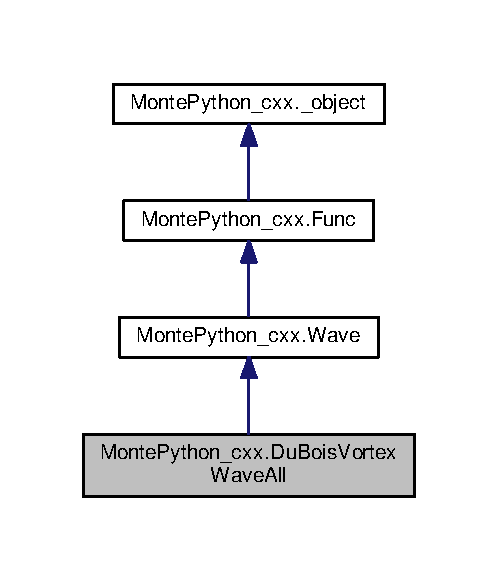
\includegraphics[width=239pt]{classMontePython__cxx_1_1DuBoisVortexWaveAll__coll__graph}
\end{center}
\end{figure}
\subsection*{Public Member Functions}
\begin{DoxyCompactItemize}
\item 
def \hyperlink{classMontePython__cxx_1_1DuBoisVortexWaveAll_ab12a62387bcfc28f3b8ebef0a3b6a7c3}{set\+Params} (self, args)
\item 
def \hyperlink{classMontePython__cxx_1_1DuBoisVortexWaveAll_ac989082a655eba12f3e818c2cc6fa82b}{value\+Pt} (self, args)
\item 
def \hyperlink{classMontePython__cxx_1_1DuBoisVortexWaveAll_aeb79cb247556ed4401c746de05ae04fa}{\+\_\+\+\_\+call\+\_\+\+\_\+} (self, args)
\item 
def \hyperlink{classMontePython__cxx_1_1DuBoisVortexWaveAll_aadfde44e0983d24ed8d1dee6e8a83ec4}{\+\_\+\+\_\+init\+\_\+\+\_\+} (self)
\end{DoxyCompactItemize}
\subsection*{Public Attributes}
\begin{DoxyCompactItemize}
\item 
\hypertarget{classMontePython__cxx_1_1DuBoisVortexWaveAll_a37f39733d1bad1ad9877f4d93c217000}{}{\bfseries this}\label{classMontePython__cxx_1_1DuBoisVortexWaveAll_a37f39733d1bad1ad9877f4d93c217000}

\end{DoxyCompactItemize}
\subsection*{Static Private Attributes}
\begin{DoxyCompactItemize}
\item 
\hypertarget{classMontePython__cxx_1_1DuBoisVortexWaveAll_af04471dea49f306acd3f38d4c4d5ae02}{}dictionary {\bfseries \+\_\+\+\_\+swig\+\_\+setmethods\+\_\+\+\_\+} = \{\}\label{classMontePython__cxx_1_1DuBoisVortexWaveAll_af04471dea49f306acd3f38d4c4d5ae02}

\item 
\hypertarget{classMontePython__cxx_1_1DuBoisVortexWaveAll_a51285ffa33b4fb32feb7a15bedd494cd}{}tuple {\bfseries \+\_\+\+\_\+setattr\+\_\+\+\_\+} = lambdaself,name,value\+:\+\_\+swig\+\_\+setattr(self, \hyperlink{classMontePython__cxx_1_1DuBoisVortexWaveAll}{Du\+Bois\+Vortex\+Wave\+All}, name, value)\label{classMontePython__cxx_1_1DuBoisVortexWaveAll_a51285ffa33b4fb32feb7a15bedd494cd}

\item 
\hypertarget{classMontePython__cxx_1_1DuBoisVortexWaveAll_afa76b6de96821f3f686fab70a47d9c22}{}dictionary {\bfseries \+\_\+\+\_\+swig\+\_\+getmethods\+\_\+\+\_\+} = \{\}\label{classMontePython__cxx_1_1DuBoisVortexWaveAll_afa76b6de96821f3f686fab70a47d9c22}

\item 
\hypertarget{classMontePython__cxx_1_1DuBoisVortexWaveAll_ad0f556f0cae614bfe6b9caa122b79c71}{}tuple {\bfseries \+\_\+\+\_\+getattr\+\_\+\+\_\+} = lambdaself,name\+:\+\_\+swig\+\_\+getattr(self, \hyperlink{classMontePython__cxx_1_1DuBoisVortexWaveAll}{Du\+Bois\+Vortex\+Wave\+All}, name)\label{classMontePython__cxx_1_1DuBoisVortexWaveAll_ad0f556f0cae614bfe6b9caa122b79c71}

\item 
\hypertarget{classMontePython__cxx_1_1DuBoisVortexWaveAll_a833adb016f67537b52f39ee195822f8f}{}{\bfseries \+\_\+\+\_\+repr\+\_\+\+\_\+} = \+\_\+swig\+\_\+repr\label{classMontePython__cxx_1_1DuBoisVortexWaveAll_a833adb016f67537b52f39ee195822f8f}

\item 
\hypertarget{classMontePython__cxx_1_1DuBoisVortexWaveAll_aa03a783e741530cc7c0a08e3cb7f95a7}{}{\bfseries \+\_\+\+\_\+swig\+\_\+destroy\+\_\+\+\_\+} = \+\_\+\+Monte\+Python\+\_\+cxx.\+delete\+\_\+\+Du\+Bois\+Vortex\+Wave\+All\label{classMontePython__cxx_1_1DuBoisVortexWaveAll_aa03a783e741530cc7c0a08e3cb7f95a7}

\end{DoxyCompactItemize}


\subsection{Detailed Description}
\begin{DoxyVerb}Proxy of C++ DuBoisVortexWaveAll class\end{DoxyVerb}
 

\subsection{Constructor \& Destructor Documentation}
\hypertarget{classMontePython__cxx_1_1DuBoisVortexWaveAll_aadfde44e0983d24ed8d1dee6e8a83ec4}{}\index{Monte\+Python\+\_\+cxx\+::\+Du\+Bois\+Vortex\+Wave\+All@{Monte\+Python\+\_\+cxx\+::\+Du\+Bois\+Vortex\+Wave\+All}!\+\_\+\+\_\+init\+\_\+\+\_\+@{\+\_\+\+\_\+init\+\_\+\+\_\+}}
\index{\+\_\+\+\_\+init\+\_\+\+\_\+@{\+\_\+\+\_\+init\+\_\+\+\_\+}!Monte\+Python\+\_\+cxx\+::\+Du\+Bois\+Vortex\+Wave\+All@{Monte\+Python\+\_\+cxx\+::\+Du\+Bois\+Vortex\+Wave\+All}}
\subsubsection[{\+\_\+\+\_\+init\+\_\+\+\_\+}]{\setlength{\rightskip}{0pt plus 5cm}def Monte\+Python\+\_\+cxx.\+Du\+Bois\+Vortex\+Wave\+All.\+\_\+\+\_\+init\+\_\+\+\_\+ (
\begin{DoxyParamCaption}
\item[{}]{self}
\end{DoxyParamCaption}
)}\label{classMontePython__cxx_1_1DuBoisVortexWaveAll_aadfde44e0983d24ed8d1dee6e8a83ec4}
\begin{DoxyVerb}__init__(DuBoisVortexWaveAll self) -> DuBoisVortexWaveAll\end{DoxyVerb}
 

\subsection{Member Function Documentation}
\hypertarget{classMontePython__cxx_1_1DuBoisVortexWaveAll_aeb79cb247556ed4401c746de05ae04fa}{}\index{Monte\+Python\+\_\+cxx\+::\+Du\+Bois\+Vortex\+Wave\+All@{Monte\+Python\+\_\+cxx\+::\+Du\+Bois\+Vortex\+Wave\+All}!\+\_\+\+\_\+call\+\_\+\+\_\+@{\+\_\+\+\_\+call\+\_\+\+\_\+}}
\index{\+\_\+\+\_\+call\+\_\+\+\_\+@{\+\_\+\+\_\+call\+\_\+\+\_\+}!Monte\+Python\+\_\+cxx\+::\+Du\+Bois\+Vortex\+Wave\+All@{Monte\+Python\+\_\+cxx\+::\+Du\+Bois\+Vortex\+Wave\+All}}
\subsubsection[{\+\_\+\+\_\+call\+\_\+\+\_\+}]{\setlength{\rightskip}{0pt plus 5cm}def Monte\+Python\+\_\+cxx.\+Du\+Bois\+Vortex\+Wave\+All.\+\_\+\+\_\+call\+\_\+\+\_\+ (
\begin{DoxyParamCaption}
\item[{}]{self, }
\item[{}]{args}
\end{DoxyParamCaption}
)}\label{classMontePython__cxx_1_1DuBoisVortexWaveAll_aeb79cb247556ed4401c746de05ae04fa}
\begin{DoxyVerb}__call__(DuBoisVortexWaveAll self, QickArray & pos) -> double\end{DoxyVerb}
 \hypertarget{classMontePython__cxx_1_1DuBoisVortexWaveAll_ab12a62387bcfc28f3b8ebef0a3b6a7c3}{}\index{Monte\+Python\+\_\+cxx\+::\+Du\+Bois\+Vortex\+Wave\+All@{Monte\+Python\+\_\+cxx\+::\+Du\+Bois\+Vortex\+Wave\+All}!set\+Params@{set\+Params}}
\index{set\+Params@{set\+Params}!Monte\+Python\+\_\+cxx\+::\+Du\+Bois\+Vortex\+Wave\+All@{Monte\+Python\+\_\+cxx\+::\+Du\+Bois\+Vortex\+Wave\+All}}
\subsubsection[{set\+Params}]{\setlength{\rightskip}{0pt plus 5cm}def Monte\+Python\+\_\+cxx.\+Du\+Bois\+Vortex\+Wave\+All.\+set\+Params (
\begin{DoxyParamCaption}
\item[{}]{self, }
\item[{}]{args}
\end{DoxyParamCaption}
)}\label{classMontePython__cxx_1_1DuBoisVortexWaveAll_ab12a62387bcfc28f3b8ebef0a3b6a7c3}
\begin{DoxyVerb}setParams(DuBoisVortexWaveAll self, QickArray & params_)\end{DoxyVerb}
 \hypertarget{classMontePython__cxx_1_1DuBoisVortexWaveAll_ac989082a655eba12f3e818c2cc6fa82b}{}\index{Monte\+Python\+\_\+cxx\+::\+Du\+Bois\+Vortex\+Wave\+All@{Monte\+Python\+\_\+cxx\+::\+Du\+Bois\+Vortex\+Wave\+All}!value\+Pt@{value\+Pt}}
\index{value\+Pt@{value\+Pt}!Monte\+Python\+\_\+cxx\+::\+Du\+Bois\+Vortex\+Wave\+All@{Monte\+Python\+\_\+cxx\+::\+Du\+Bois\+Vortex\+Wave\+All}}
\subsubsection[{value\+Pt}]{\setlength{\rightskip}{0pt plus 5cm}def Monte\+Python\+\_\+cxx.\+Du\+Bois\+Vortex\+Wave\+All.\+value\+Pt (
\begin{DoxyParamCaption}
\item[{}]{self, }
\item[{}]{args}
\end{DoxyParamCaption}
)}\label{classMontePython__cxx_1_1DuBoisVortexWaveAll_ac989082a655eba12f3e818c2cc6fa82b}
\begin{DoxyVerb}valuePt(DuBoisVortexWaveAll self, QickArray & pos) -> double\end{DoxyVerb}
 

The documentation for this class was generated from the following file\+:\begin{DoxyCompactItemize}
\item 
Monte\+Python\+\_\+cxx.\+py\end{DoxyCompactItemize}

\hypertarget{classMontePython__cxx_1_1DuBoisWave}{}\section{Monte\+Python\+\_\+cxx.\+Du\+Bois\+Wave Class Reference}
\label{classMontePython__cxx_1_1DuBoisWave}\index{Monte\+Python\+\_\+cxx.\+Du\+Bois\+Wave@{Monte\+Python\+\_\+cxx.\+Du\+Bois\+Wave}}


Inheritance diagram for Monte\+Python\+\_\+cxx.\+Du\+Bois\+Wave\+:
\nopagebreak
\begin{figure}[H]
\begin{center}
\leavevmode
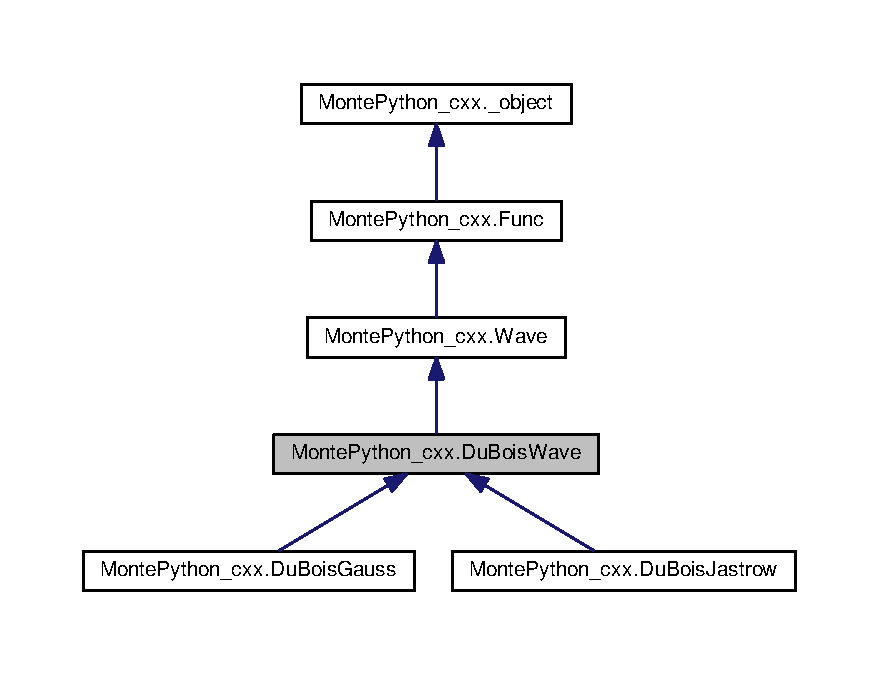
\includegraphics[width=350pt]{classMontePython__cxx_1_1DuBoisWave__inherit__graph}
\end{center}
\end{figure}


Collaboration diagram for Monte\+Python\+\_\+cxx.\+Du\+Bois\+Wave\+:
\nopagebreak
\begin{figure}[H]
\begin{center}
\leavevmode
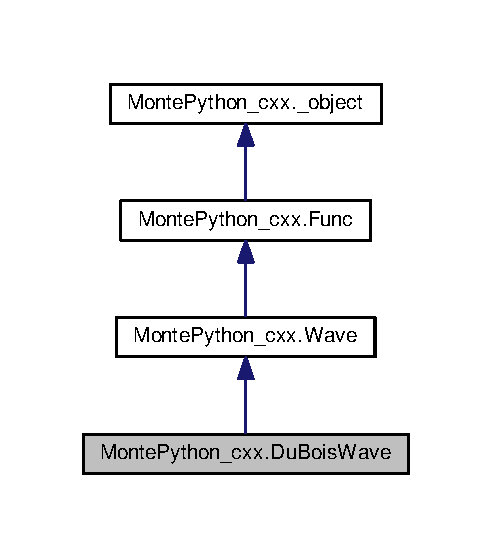
\includegraphics[width=236pt]{classMontePython__cxx_1_1DuBoisWave__coll__graph}
\end{center}
\end{figure}
\subsection*{Public Member Functions}
\begin{DoxyCompactItemize}
\item 
def \hyperlink{classMontePython__cxx_1_1DuBoisWave_a2274beece9d7d2ed7f7fdf0ae619e5e7}{set\+Params} (self, args)
\item 
def \hyperlink{classMontePython__cxx_1_1DuBoisWave_a3ce97c646707c488d1601e82fd28bce7}{value\+Pt} (self, args)
\item 
def \hyperlink{classMontePython__cxx_1_1DuBoisWave_a897d63f5ee2e5050b8742441ec1e26f9}{\+\_\+\+\_\+call\+\_\+\+\_\+} (self, args)
\item 
def \hyperlink{classMontePython__cxx_1_1DuBoisWave_a69ea0eb80b4c1db4a3dce6f20d916025}{\+\_\+\+\_\+init\+\_\+\+\_\+} (self)
\end{DoxyCompactItemize}
\subsection*{Public Attributes}
\begin{DoxyCompactItemize}
\item 
\hypertarget{classMontePython__cxx_1_1DuBoisWave_a3f1e7f312ea894811e5a368620b73ead}{}{\bfseries this}\label{classMontePython__cxx_1_1DuBoisWave_a3f1e7f312ea894811e5a368620b73ead}

\end{DoxyCompactItemize}
\subsection*{Static Private Attributes}
\begin{DoxyCompactItemize}
\item 
\hypertarget{classMontePython__cxx_1_1DuBoisWave_a7d6fb9dfe2f1da070d6447f999d2533a}{}dictionary {\bfseries \+\_\+\+\_\+swig\+\_\+setmethods\+\_\+\+\_\+} = \{\}\label{classMontePython__cxx_1_1DuBoisWave_a7d6fb9dfe2f1da070d6447f999d2533a}

\item 
\hypertarget{classMontePython__cxx_1_1DuBoisWave_a2f1d1f3ab2ea3add6915de83c41d34d5}{}tuple {\bfseries \+\_\+\+\_\+setattr\+\_\+\+\_\+} = lambdaself,name,value\+:\+\_\+swig\+\_\+setattr(self, \hyperlink{classMontePython__cxx_1_1DuBoisWave}{Du\+Bois\+Wave}, name, value)\label{classMontePython__cxx_1_1DuBoisWave_a2f1d1f3ab2ea3add6915de83c41d34d5}

\item 
\hypertarget{classMontePython__cxx_1_1DuBoisWave_a2ff16ff62f8f554cff1c97670bd02d6d}{}dictionary {\bfseries \+\_\+\+\_\+swig\+\_\+getmethods\+\_\+\+\_\+} = \{\}\label{classMontePython__cxx_1_1DuBoisWave_a2ff16ff62f8f554cff1c97670bd02d6d}

\item 
\hypertarget{classMontePython__cxx_1_1DuBoisWave_ac641e8db1a1acd606852ed6555a77eb5}{}tuple {\bfseries \+\_\+\+\_\+getattr\+\_\+\+\_\+} = lambdaself,name\+:\+\_\+swig\+\_\+getattr(self, \hyperlink{classMontePython__cxx_1_1DuBoisWave}{Du\+Bois\+Wave}, name)\label{classMontePython__cxx_1_1DuBoisWave_ac641e8db1a1acd606852ed6555a77eb5}

\item 
\hypertarget{classMontePython__cxx_1_1DuBoisWave_a9e0d5521e7c38b109dfd882907dc6461}{}{\bfseries \+\_\+\+\_\+repr\+\_\+\+\_\+} = \+\_\+swig\+\_\+repr\label{classMontePython__cxx_1_1DuBoisWave_a9e0d5521e7c38b109dfd882907dc6461}

\item 
\hypertarget{classMontePython__cxx_1_1DuBoisWave_a32e5a094fb95974ec7ea76f18872dd96}{}{\bfseries \+\_\+\+\_\+swig\+\_\+destroy\+\_\+\+\_\+} = \+\_\+\+Monte\+Python\+\_\+cxx.\+delete\+\_\+\+Du\+Bois\+Wave\label{classMontePython__cxx_1_1DuBoisWave_a32e5a094fb95974ec7ea76f18872dd96}

\end{DoxyCompactItemize}


\subsection{Detailed Description}
\begin{DoxyVerb}Proxy of C++ DuBoisWave class\end{DoxyVerb}
 

\subsection{Constructor \& Destructor Documentation}
\hypertarget{classMontePython__cxx_1_1DuBoisWave_a69ea0eb80b4c1db4a3dce6f20d916025}{}\index{Monte\+Python\+\_\+cxx\+::\+Du\+Bois\+Wave@{Monte\+Python\+\_\+cxx\+::\+Du\+Bois\+Wave}!\+\_\+\+\_\+init\+\_\+\+\_\+@{\+\_\+\+\_\+init\+\_\+\+\_\+}}
\index{\+\_\+\+\_\+init\+\_\+\+\_\+@{\+\_\+\+\_\+init\+\_\+\+\_\+}!Monte\+Python\+\_\+cxx\+::\+Du\+Bois\+Wave@{Monte\+Python\+\_\+cxx\+::\+Du\+Bois\+Wave}}
\subsubsection[{\+\_\+\+\_\+init\+\_\+\+\_\+}]{\setlength{\rightskip}{0pt plus 5cm}def Monte\+Python\+\_\+cxx.\+Du\+Bois\+Wave.\+\_\+\+\_\+init\+\_\+\+\_\+ (
\begin{DoxyParamCaption}
\item[{}]{self}
\end{DoxyParamCaption}
)}\label{classMontePython__cxx_1_1DuBoisWave_a69ea0eb80b4c1db4a3dce6f20d916025}
\begin{DoxyVerb}__init__(DuBoisWave self) -> DuBoisWave\end{DoxyVerb}
 

\subsection{Member Function Documentation}
\hypertarget{classMontePython__cxx_1_1DuBoisWave_a897d63f5ee2e5050b8742441ec1e26f9}{}\index{Monte\+Python\+\_\+cxx\+::\+Du\+Bois\+Wave@{Monte\+Python\+\_\+cxx\+::\+Du\+Bois\+Wave}!\+\_\+\+\_\+call\+\_\+\+\_\+@{\+\_\+\+\_\+call\+\_\+\+\_\+}}
\index{\+\_\+\+\_\+call\+\_\+\+\_\+@{\+\_\+\+\_\+call\+\_\+\+\_\+}!Monte\+Python\+\_\+cxx\+::\+Du\+Bois\+Wave@{Monte\+Python\+\_\+cxx\+::\+Du\+Bois\+Wave}}
\subsubsection[{\+\_\+\+\_\+call\+\_\+\+\_\+}]{\setlength{\rightskip}{0pt plus 5cm}def Monte\+Python\+\_\+cxx.\+Du\+Bois\+Wave.\+\_\+\+\_\+call\+\_\+\+\_\+ (
\begin{DoxyParamCaption}
\item[{}]{self, }
\item[{}]{args}
\end{DoxyParamCaption}
)}\label{classMontePython__cxx_1_1DuBoisWave_a897d63f5ee2e5050b8742441ec1e26f9}
\begin{DoxyVerb}__call__(DuBoisWave self, QickArray & pos) -> double\end{DoxyVerb}
 \hypertarget{classMontePython__cxx_1_1DuBoisWave_a2274beece9d7d2ed7f7fdf0ae619e5e7}{}\index{Monte\+Python\+\_\+cxx\+::\+Du\+Bois\+Wave@{Monte\+Python\+\_\+cxx\+::\+Du\+Bois\+Wave}!set\+Params@{set\+Params}}
\index{set\+Params@{set\+Params}!Monte\+Python\+\_\+cxx\+::\+Du\+Bois\+Wave@{Monte\+Python\+\_\+cxx\+::\+Du\+Bois\+Wave}}
\subsubsection[{set\+Params}]{\setlength{\rightskip}{0pt plus 5cm}def Monte\+Python\+\_\+cxx.\+Du\+Bois\+Wave.\+set\+Params (
\begin{DoxyParamCaption}
\item[{}]{self, }
\item[{}]{args}
\end{DoxyParamCaption}
)}\label{classMontePython__cxx_1_1DuBoisWave_a2274beece9d7d2ed7f7fdf0ae619e5e7}
\begin{DoxyVerb}setParams(DuBoisWave self, QickArray & params_)\end{DoxyVerb}
 \hypertarget{classMontePython__cxx_1_1DuBoisWave_a3ce97c646707c488d1601e82fd28bce7}{}\index{Monte\+Python\+\_\+cxx\+::\+Du\+Bois\+Wave@{Monte\+Python\+\_\+cxx\+::\+Du\+Bois\+Wave}!value\+Pt@{value\+Pt}}
\index{value\+Pt@{value\+Pt}!Monte\+Python\+\_\+cxx\+::\+Du\+Bois\+Wave@{Monte\+Python\+\_\+cxx\+::\+Du\+Bois\+Wave}}
\subsubsection[{value\+Pt}]{\setlength{\rightskip}{0pt plus 5cm}def Monte\+Python\+\_\+cxx.\+Du\+Bois\+Wave.\+value\+Pt (
\begin{DoxyParamCaption}
\item[{}]{self, }
\item[{}]{args}
\end{DoxyParamCaption}
)}\label{classMontePython__cxx_1_1DuBoisWave_a3ce97c646707c488d1601e82fd28bce7}
\begin{DoxyVerb}valuePt(DuBoisWave self, QickArray & pos) -> double\end{DoxyVerb}
 

The documentation for this class was generated from the following file\+:\begin{DoxyCompactItemize}
\item 
Monte\+Python\+\_\+cxx.\+py\end{DoxyCompactItemize}

\hypertarget{classMontePython__cxx_1_1DuBoisWaveAll}{}\section{Monte\+Python\+\_\+cxx.\+Du\+Bois\+Wave\+All Class Reference}
\label{classMontePython__cxx_1_1DuBoisWaveAll}\index{Monte\+Python\+\_\+cxx.\+Du\+Bois\+Wave\+All@{Monte\+Python\+\_\+cxx.\+Du\+Bois\+Wave\+All}}


Inheritance diagram for Monte\+Python\+\_\+cxx.\+Du\+Bois\+Wave\+All\+:
\nopagebreak
\begin{figure}[H]
\begin{center}
\leavevmode
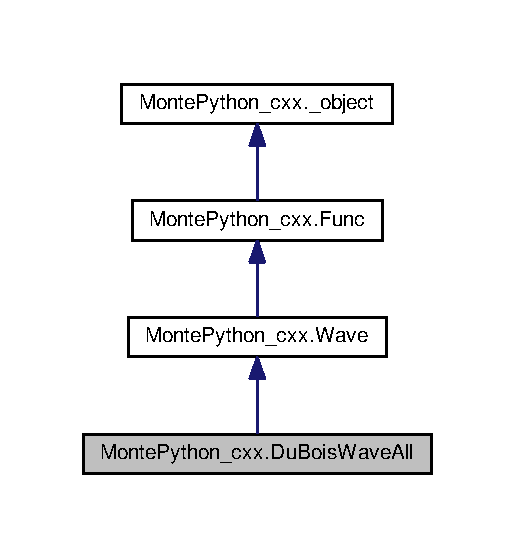
\includegraphics[width=247pt]{classMontePython__cxx_1_1DuBoisWaveAll__inherit__graph}
\end{center}
\end{figure}


Collaboration diagram for Monte\+Python\+\_\+cxx.\+Du\+Bois\+Wave\+All\+:
\nopagebreak
\begin{figure}[H]
\begin{center}
\leavevmode
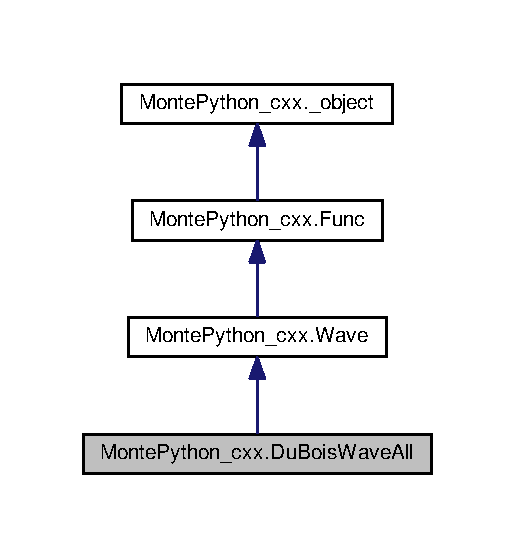
\includegraphics[width=247pt]{classMontePython__cxx_1_1DuBoisWaveAll__coll__graph}
\end{center}
\end{figure}
\subsection*{Public Member Functions}
\begin{DoxyCompactItemize}
\item 
def \hyperlink{classMontePython__cxx_1_1DuBoisWaveAll_a940a91f9bc21bc8b5f821294bae3b95a}{set\+Params} (self, args)
\item 
def \hyperlink{classMontePython__cxx_1_1DuBoisWaveAll_af33d930a76d1e703ac44883e96669c4f}{value\+Pt} (self, args)
\item 
def \hyperlink{classMontePython__cxx_1_1DuBoisWaveAll_aae04493077d640185d3937ff1f6cf147}{\+\_\+\+\_\+call\+\_\+\+\_\+} (self, args)
\item 
def \hyperlink{classMontePython__cxx_1_1DuBoisWaveAll_a6dd09776e1284edc54cf9a45e2a71deb}{\+\_\+\+\_\+init\+\_\+\+\_\+} (self)
\end{DoxyCompactItemize}
\subsection*{Public Attributes}
\begin{DoxyCompactItemize}
\item 
\hypertarget{classMontePython__cxx_1_1DuBoisWaveAll_a82b04cfd847af964769548c4a8aebaaa}{}{\bfseries this}\label{classMontePython__cxx_1_1DuBoisWaveAll_a82b04cfd847af964769548c4a8aebaaa}

\end{DoxyCompactItemize}
\subsection*{Static Private Attributes}
\begin{DoxyCompactItemize}
\item 
\hypertarget{classMontePython__cxx_1_1DuBoisWaveAll_ae7869eebda916be712b61c3200b12e19}{}dictionary {\bfseries \+\_\+\+\_\+swig\+\_\+setmethods\+\_\+\+\_\+} = \{\}\label{classMontePython__cxx_1_1DuBoisWaveAll_ae7869eebda916be712b61c3200b12e19}

\item 
\hypertarget{classMontePython__cxx_1_1DuBoisWaveAll_a9925f24332ccfc0b7affe981f1883b70}{}tuple {\bfseries \+\_\+\+\_\+setattr\+\_\+\+\_\+} = lambdaself,name,value\+:\+\_\+swig\+\_\+setattr(self, \hyperlink{classMontePython__cxx_1_1DuBoisWaveAll}{Du\+Bois\+Wave\+All}, name, value)\label{classMontePython__cxx_1_1DuBoisWaveAll_a9925f24332ccfc0b7affe981f1883b70}

\item 
\hypertarget{classMontePython__cxx_1_1DuBoisWaveAll_ab606da2bec42245cc38398c597464b91}{}dictionary {\bfseries \+\_\+\+\_\+swig\+\_\+getmethods\+\_\+\+\_\+} = \{\}\label{classMontePython__cxx_1_1DuBoisWaveAll_ab606da2bec42245cc38398c597464b91}

\item 
\hypertarget{classMontePython__cxx_1_1DuBoisWaveAll_af812e052a7c12d75d0e3d06f1f228fbf}{}tuple {\bfseries \+\_\+\+\_\+getattr\+\_\+\+\_\+} = lambdaself,name\+:\+\_\+swig\+\_\+getattr(self, \hyperlink{classMontePython__cxx_1_1DuBoisWaveAll}{Du\+Bois\+Wave\+All}, name)\label{classMontePython__cxx_1_1DuBoisWaveAll_af812e052a7c12d75d0e3d06f1f228fbf}

\item 
\hypertarget{classMontePython__cxx_1_1DuBoisWaveAll_a544218b3434ac8e35bd07abad3debca4}{}{\bfseries \+\_\+\+\_\+repr\+\_\+\+\_\+} = \+\_\+swig\+\_\+repr\label{classMontePython__cxx_1_1DuBoisWaveAll_a544218b3434ac8e35bd07abad3debca4}

\item 
\hypertarget{classMontePython__cxx_1_1DuBoisWaveAll_a4656662c8f98d62cc2b10ebeb0d0eae7}{}{\bfseries \+\_\+\+\_\+swig\+\_\+destroy\+\_\+\+\_\+} = \+\_\+\+Monte\+Python\+\_\+cxx.\+delete\+\_\+\+Du\+Bois\+Wave\+All\label{classMontePython__cxx_1_1DuBoisWaveAll_a4656662c8f98d62cc2b10ebeb0d0eae7}

\end{DoxyCompactItemize}


\subsection{Detailed Description}
\begin{DoxyVerb}Proxy of C++ DuBoisWaveAll class\end{DoxyVerb}
 

\subsection{Constructor \& Destructor Documentation}
\hypertarget{classMontePython__cxx_1_1DuBoisWaveAll_a6dd09776e1284edc54cf9a45e2a71deb}{}\index{Monte\+Python\+\_\+cxx\+::\+Du\+Bois\+Wave\+All@{Monte\+Python\+\_\+cxx\+::\+Du\+Bois\+Wave\+All}!\+\_\+\+\_\+init\+\_\+\+\_\+@{\+\_\+\+\_\+init\+\_\+\+\_\+}}
\index{\+\_\+\+\_\+init\+\_\+\+\_\+@{\+\_\+\+\_\+init\+\_\+\+\_\+}!Monte\+Python\+\_\+cxx\+::\+Du\+Bois\+Wave\+All@{Monte\+Python\+\_\+cxx\+::\+Du\+Bois\+Wave\+All}}
\subsubsection[{\+\_\+\+\_\+init\+\_\+\+\_\+}]{\setlength{\rightskip}{0pt plus 5cm}def Monte\+Python\+\_\+cxx.\+Du\+Bois\+Wave\+All.\+\_\+\+\_\+init\+\_\+\+\_\+ (
\begin{DoxyParamCaption}
\item[{}]{self}
\end{DoxyParamCaption}
)}\label{classMontePython__cxx_1_1DuBoisWaveAll_a6dd09776e1284edc54cf9a45e2a71deb}
\begin{DoxyVerb}__init__(DuBoisWaveAll self) -> DuBoisWaveAll\end{DoxyVerb}
 

\subsection{Member Function Documentation}
\hypertarget{classMontePython__cxx_1_1DuBoisWaveAll_aae04493077d640185d3937ff1f6cf147}{}\index{Monte\+Python\+\_\+cxx\+::\+Du\+Bois\+Wave\+All@{Monte\+Python\+\_\+cxx\+::\+Du\+Bois\+Wave\+All}!\+\_\+\+\_\+call\+\_\+\+\_\+@{\+\_\+\+\_\+call\+\_\+\+\_\+}}
\index{\+\_\+\+\_\+call\+\_\+\+\_\+@{\+\_\+\+\_\+call\+\_\+\+\_\+}!Monte\+Python\+\_\+cxx\+::\+Du\+Bois\+Wave\+All@{Monte\+Python\+\_\+cxx\+::\+Du\+Bois\+Wave\+All}}
\subsubsection[{\+\_\+\+\_\+call\+\_\+\+\_\+}]{\setlength{\rightskip}{0pt plus 5cm}def Monte\+Python\+\_\+cxx.\+Du\+Bois\+Wave\+All.\+\_\+\+\_\+call\+\_\+\+\_\+ (
\begin{DoxyParamCaption}
\item[{}]{self, }
\item[{}]{args}
\end{DoxyParamCaption}
)}\label{classMontePython__cxx_1_1DuBoisWaveAll_aae04493077d640185d3937ff1f6cf147}
\begin{DoxyVerb}__call__(DuBoisWaveAll self, QickArray & pos) -> double\end{DoxyVerb}
 \hypertarget{classMontePython__cxx_1_1DuBoisWaveAll_a940a91f9bc21bc8b5f821294bae3b95a}{}\index{Monte\+Python\+\_\+cxx\+::\+Du\+Bois\+Wave\+All@{Monte\+Python\+\_\+cxx\+::\+Du\+Bois\+Wave\+All}!set\+Params@{set\+Params}}
\index{set\+Params@{set\+Params}!Monte\+Python\+\_\+cxx\+::\+Du\+Bois\+Wave\+All@{Monte\+Python\+\_\+cxx\+::\+Du\+Bois\+Wave\+All}}
\subsubsection[{set\+Params}]{\setlength{\rightskip}{0pt plus 5cm}def Monte\+Python\+\_\+cxx.\+Du\+Bois\+Wave\+All.\+set\+Params (
\begin{DoxyParamCaption}
\item[{}]{self, }
\item[{}]{args}
\end{DoxyParamCaption}
)}\label{classMontePython__cxx_1_1DuBoisWaveAll_a940a91f9bc21bc8b5f821294bae3b95a}
\begin{DoxyVerb}setParams(DuBoisWaveAll self, QickArray & params_)\end{DoxyVerb}
 \hypertarget{classMontePython__cxx_1_1DuBoisWaveAll_af33d930a76d1e703ac44883e96669c4f}{}\index{Monte\+Python\+\_\+cxx\+::\+Du\+Bois\+Wave\+All@{Monte\+Python\+\_\+cxx\+::\+Du\+Bois\+Wave\+All}!value\+Pt@{value\+Pt}}
\index{value\+Pt@{value\+Pt}!Monte\+Python\+\_\+cxx\+::\+Du\+Bois\+Wave\+All@{Monte\+Python\+\_\+cxx\+::\+Du\+Bois\+Wave\+All}}
\subsubsection[{value\+Pt}]{\setlength{\rightskip}{0pt plus 5cm}def Monte\+Python\+\_\+cxx.\+Du\+Bois\+Wave\+All.\+value\+Pt (
\begin{DoxyParamCaption}
\item[{}]{self, }
\item[{}]{args}
\end{DoxyParamCaption}
)}\label{classMontePython__cxx_1_1DuBoisWaveAll_af33d930a76d1e703ac44883e96669c4f}
\begin{DoxyVerb}valuePt(DuBoisWaveAll self, QickArray & pos) -> double\end{DoxyVerb}
 

The documentation for this class was generated from the following file\+:\begin{DoxyCompactItemize}
\item 
Monte\+Python\+\_\+cxx.\+py\end{DoxyCompactItemize}

\hypertarget{classMontePython__cxx_1_1Func}{}\section{Monte\+Python\+\_\+cxx.\+Func Class Reference}
\label{classMontePython__cxx_1_1Func}\index{Monte\+Python\+\_\+cxx.\+Func@{Monte\+Python\+\_\+cxx.\+Func}}


Inheritance diagram for Monte\+Python\+\_\+cxx.\+Func\+:
\nopagebreak
\begin{figure}[H]
\begin{center}
\leavevmode
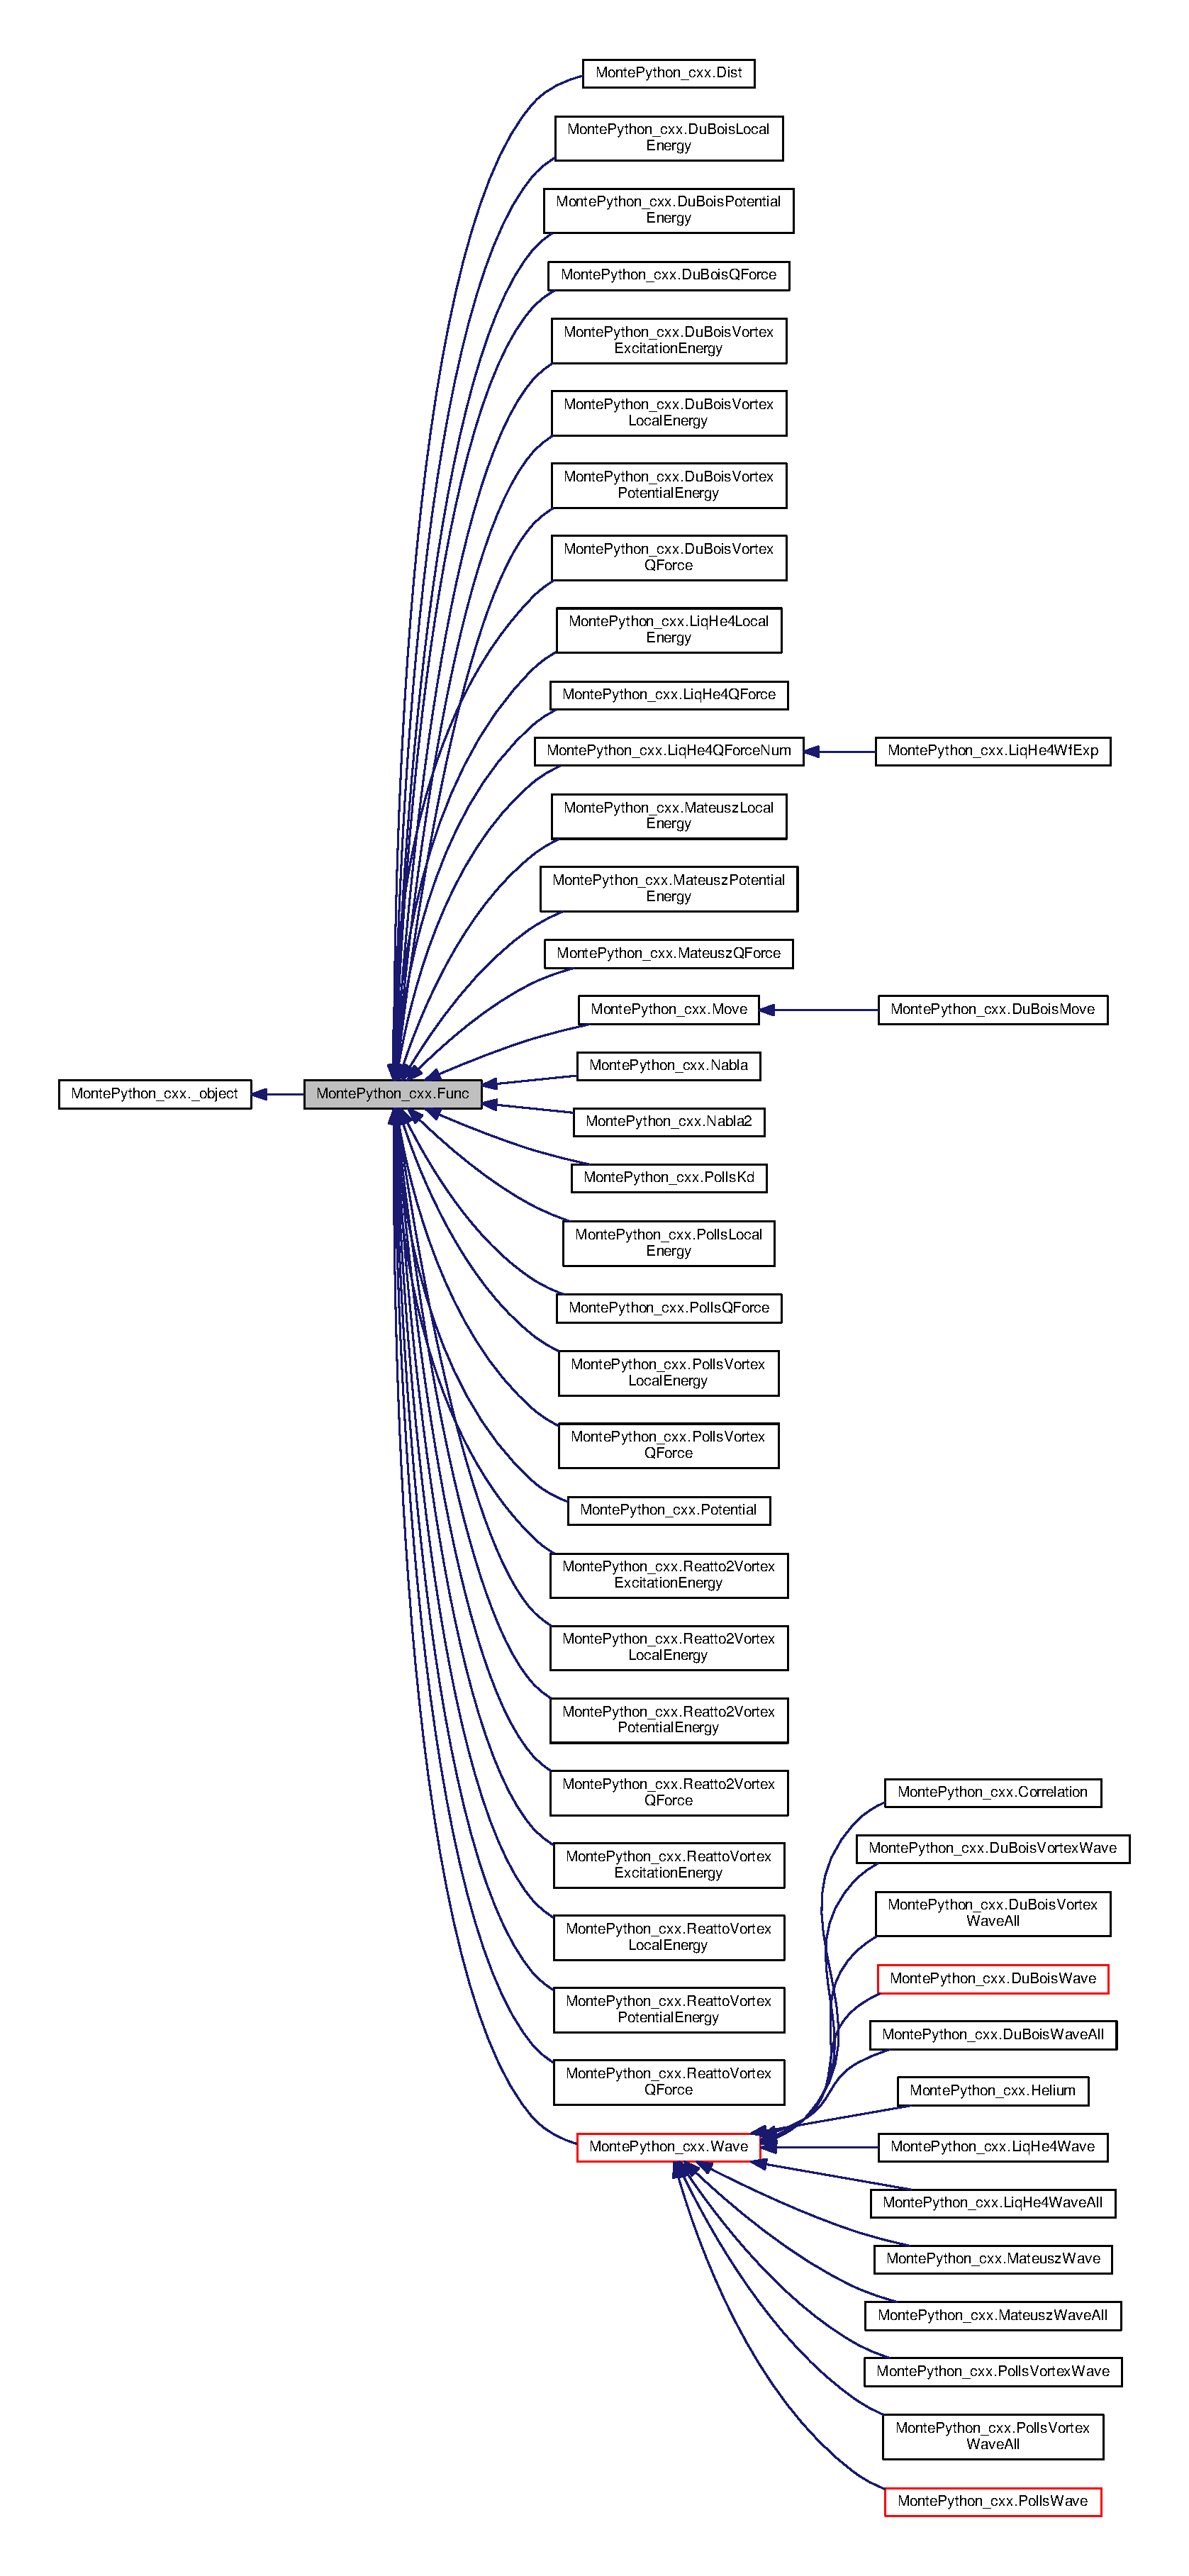
\includegraphics[height=550pt]{classMontePython__cxx_1_1Func__inherit__graph}
\end{center}
\end{figure}


Collaboration diagram for Monte\+Python\+\_\+cxx.\+Func\+:
\nopagebreak
\begin{figure}[H]
\begin{center}
\leavevmode
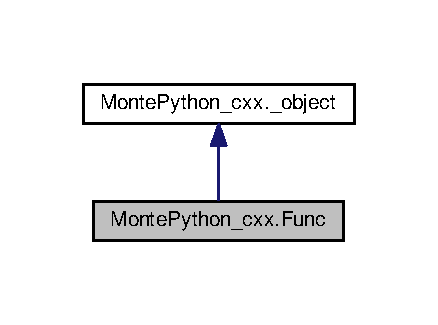
\includegraphics[width=210pt]{classMontePython__cxx_1_1Func__coll__graph}
\end{center}
\end{figure}
\subsection*{Public Member Functions}
\begin{DoxyCompactItemize}
\item 
def \hyperlink{classMontePython__cxx_1_1Func_a84b9bc6208735485c30d1b21182ed81f}{set\+Params} (self, args)
\item 
def \hyperlink{classMontePython__cxx_1_1Func_a6a6ab69fac1f1629d90499011237c631}{get\+Impossible} (self)
\item 
def \hyperlink{classMontePython__cxx_1_1Func_a53476af0f03d502c63a4ae2a65f4a0b7}{value\+Pt} (self, args)
\item 
def \hyperlink{classMontePython__cxx_1_1Func_a9ca4408c85ae96c8feae3f20bb288144}{\+\_\+\+\_\+call\+\_\+\+\_\+} (self, args)
\item 
def \hyperlink{classMontePython__cxx_1_1Func_ad38accd52a7370704b5482e6dbcb88cb}{sqr} (self, args)
\item 
def \hyperlink{classMontePython__cxx_1_1Func_a09bc358cbee40b7e742c474cb3d8cd8c}{\+\_\+\+\_\+init\+\_\+\+\_\+} (self)
\end{DoxyCompactItemize}
\subsection*{Public Attributes}
\begin{DoxyCompactItemize}
\item 
\hypertarget{classMontePython__cxx_1_1Func_ad3085ee8b7efab758df39e0970220b8f}{}{\bfseries this}\label{classMontePython__cxx_1_1Func_ad3085ee8b7efab758df39e0970220b8f}

\end{DoxyCompactItemize}
\subsection*{Static Private Attributes}
\begin{DoxyCompactItemize}
\item 
\hypertarget{classMontePython__cxx_1_1Func_acc8467835ccaf51d589694f96ecdd97c}{}dictionary {\bfseries \+\_\+\+\_\+swig\+\_\+setmethods\+\_\+\+\_\+} = \{\}\label{classMontePython__cxx_1_1Func_acc8467835ccaf51d589694f96ecdd97c}

\item 
\hypertarget{classMontePython__cxx_1_1Func_a457342b683008ffdf90e97b30c3e10fb}{}tuple {\bfseries \+\_\+\+\_\+setattr\+\_\+\+\_\+} = lambdaself,name,value\+:\+\_\+swig\+\_\+setattr(self, \hyperlink{classMontePython__cxx_1_1Func}{Func}, name, value)\label{classMontePython__cxx_1_1Func_a457342b683008ffdf90e97b30c3e10fb}

\item 
\hypertarget{classMontePython__cxx_1_1Func_aaef40405a6d762fce14f2322452de850}{}dictionary {\bfseries \+\_\+\+\_\+swig\+\_\+getmethods\+\_\+\+\_\+} = \{\}\label{classMontePython__cxx_1_1Func_aaef40405a6d762fce14f2322452de850}

\item 
\hypertarget{classMontePython__cxx_1_1Func_a4d48a675dbe5edcb31f14859e854e623}{}tuple {\bfseries \+\_\+\+\_\+getattr\+\_\+\+\_\+} = lambdaself,name\+:\+\_\+swig\+\_\+getattr(self, \hyperlink{classMontePython__cxx_1_1Func}{Func}, name)\label{classMontePython__cxx_1_1Func_a4d48a675dbe5edcb31f14859e854e623}

\item 
\hypertarget{classMontePython__cxx_1_1Func_a6ef995a5f62c27f14e6582f2364b1a93}{}{\bfseries \+\_\+\+\_\+repr\+\_\+\+\_\+} = \+\_\+swig\+\_\+repr\label{classMontePython__cxx_1_1Func_a6ef995a5f62c27f14e6582f2364b1a93}

\item 
\hypertarget{classMontePython__cxx_1_1Func_abc63cc68234e25e9aa81216559b28d11}{}{\bfseries \+\_\+\+\_\+swig\+\_\+destroy\+\_\+\+\_\+} = \+\_\+\+Monte\+Python\+\_\+cxx.\+delete\+\_\+\+Func\label{classMontePython__cxx_1_1Func_abc63cc68234e25e9aa81216559b28d11}

\item 
\hypertarget{classMontePython__cxx_1_1Func_aa9b7f85168babb643a6264c1c4c5e1db}{}{\bfseries \+\_\+\+\_\+del\+\_\+\+\_\+} = lambdaself\+:\+None;\label{classMontePython__cxx_1_1Func_aa9b7f85168babb643a6264c1c4c5e1db}

\end{DoxyCompactItemize}


\subsection{Detailed Description}
\begin{DoxyVerb}Proxy of C++ Func class\end{DoxyVerb}
 

\subsection{Constructor \& Destructor Documentation}
\hypertarget{classMontePython__cxx_1_1Func_a09bc358cbee40b7e742c474cb3d8cd8c}{}\index{Monte\+Python\+\_\+cxx\+::\+Func@{Monte\+Python\+\_\+cxx\+::\+Func}!\+\_\+\+\_\+init\+\_\+\+\_\+@{\+\_\+\+\_\+init\+\_\+\+\_\+}}
\index{\+\_\+\+\_\+init\+\_\+\+\_\+@{\+\_\+\+\_\+init\+\_\+\+\_\+}!Monte\+Python\+\_\+cxx\+::\+Func@{Monte\+Python\+\_\+cxx\+::\+Func}}
\subsubsection[{\+\_\+\+\_\+init\+\_\+\+\_\+}]{\setlength{\rightskip}{0pt plus 5cm}def Monte\+Python\+\_\+cxx.\+Func.\+\_\+\+\_\+init\+\_\+\+\_\+ (
\begin{DoxyParamCaption}
\item[{}]{self}
\end{DoxyParamCaption}
)}\label{classMontePython__cxx_1_1Func_a09bc358cbee40b7e742c474cb3d8cd8c}
\begin{DoxyVerb}__init__(Func self) -> Func\end{DoxyVerb}
 

\subsection{Member Function Documentation}
\hypertarget{classMontePython__cxx_1_1Func_a9ca4408c85ae96c8feae3f20bb288144}{}\index{Monte\+Python\+\_\+cxx\+::\+Func@{Monte\+Python\+\_\+cxx\+::\+Func}!\+\_\+\+\_\+call\+\_\+\+\_\+@{\+\_\+\+\_\+call\+\_\+\+\_\+}}
\index{\+\_\+\+\_\+call\+\_\+\+\_\+@{\+\_\+\+\_\+call\+\_\+\+\_\+}!Monte\+Python\+\_\+cxx\+::\+Func@{Monte\+Python\+\_\+cxx\+::\+Func}}
\subsubsection[{\+\_\+\+\_\+call\+\_\+\+\_\+}]{\setlength{\rightskip}{0pt plus 5cm}def Monte\+Python\+\_\+cxx.\+Func.\+\_\+\+\_\+call\+\_\+\+\_\+ (
\begin{DoxyParamCaption}
\item[{}]{self, }
\item[{}]{args}
\end{DoxyParamCaption}
)}\label{classMontePython__cxx_1_1Func_a9ca4408c85ae96c8feae3f20bb288144}
\begin{DoxyVerb}__call__(Func self, double x, double y) -> double
__call__(Func self, QickArray & pos) -> double
__call__(Func self, QickArray & pos, int i, Random ran) -> QickArray
__call__(Func self, QickArray & pos, int i, QickArray & x, Random ran) -> QickArray
__call__(Func self, QickArray & pos, bool dummy) -> QickArray
__call__(Func self, Func func, QickArray & pos) -> double
__call__(Func self, QickArray & pos, Func func) -> QickArray
__call__(Func self, QickArray & pos, double x) -> QickArray &
\end{DoxyVerb}
 \hypertarget{classMontePython__cxx_1_1Func_a6a6ab69fac1f1629d90499011237c631}{}\index{Monte\+Python\+\_\+cxx\+::\+Func@{Monte\+Python\+\_\+cxx\+::\+Func}!get\+Impossible@{get\+Impossible}}
\index{get\+Impossible@{get\+Impossible}!Monte\+Python\+\_\+cxx\+::\+Func@{Monte\+Python\+\_\+cxx\+::\+Func}}
\subsubsection[{get\+Impossible}]{\setlength{\rightskip}{0pt plus 5cm}def Monte\+Python\+\_\+cxx.\+Func.\+get\+Impossible (
\begin{DoxyParamCaption}
\item[{}]{self}
\end{DoxyParamCaption}
)}\label{classMontePython__cxx_1_1Func_a6a6ab69fac1f1629d90499011237c631}
\begin{DoxyVerb}getImpossible(Func self) -> bool\end{DoxyVerb}
 \hypertarget{classMontePython__cxx_1_1Func_a84b9bc6208735485c30d1b21182ed81f}{}\index{Monte\+Python\+\_\+cxx\+::\+Func@{Monte\+Python\+\_\+cxx\+::\+Func}!set\+Params@{set\+Params}}
\index{set\+Params@{set\+Params}!Monte\+Python\+\_\+cxx\+::\+Func@{Monte\+Python\+\_\+cxx\+::\+Func}}
\subsubsection[{set\+Params}]{\setlength{\rightskip}{0pt plus 5cm}def Monte\+Python\+\_\+cxx.\+Func.\+set\+Params (
\begin{DoxyParamCaption}
\item[{}]{self, }
\item[{}]{args}
\end{DoxyParamCaption}
)}\label{classMontePython__cxx_1_1Func_a84b9bc6208735485c30d1b21182ed81f}
\begin{DoxyVerb}setParams(Func self, QickArray & params_)\end{DoxyVerb}
 \hypertarget{classMontePython__cxx_1_1Func_ad38accd52a7370704b5482e6dbcb88cb}{}\index{Monte\+Python\+\_\+cxx\+::\+Func@{Monte\+Python\+\_\+cxx\+::\+Func}!sqr@{sqr}}
\index{sqr@{sqr}!Monte\+Python\+\_\+cxx\+::\+Func@{Monte\+Python\+\_\+cxx\+::\+Func}}
\subsubsection[{sqr}]{\setlength{\rightskip}{0pt plus 5cm}def Monte\+Python\+\_\+cxx.\+Func.\+sqr (
\begin{DoxyParamCaption}
\item[{}]{self, }
\item[{}]{args}
\end{DoxyParamCaption}
)}\label{classMontePython__cxx_1_1Func_ad38accd52a7370704b5482e6dbcb88cb}
\begin{DoxyVerb}sqr(Func self, double x) -> double\end{DoxyVerb}
 \hypertarget{classMontePython__cxx_1_1Func_a53476af0f03d502c63a4ae2a65f4a0b7}{}\index{Monte\+Python\+\_\+cxx\+::\+Func@{Monte\+Python\+\_\+cxx\+::\+Func}!value\+Pt@{value\+Pt}}
\index{value\+Pt@{value\+Pt}!Monte\+Python\+\_\+cxx\+::\+Func@{Monte\+Python\+\_\+cxx\+::\+Func}}
\subsubsection[{value\+Pt}]{\setlength{\rightskip}{0pt plus 5cm}def Monte\+Python\+\_\+cxx.\+Func.\+value\+Pt (
\begin{DoxyParamCaption}
\item[{}]{self, }
\item[{}]{args}
\end{DoxyParamCaption}
)}\label{classMontePython__cxx_1_1Func_a53476af0f03d502c63a4ae2a65f4a0b7}
\begin{DoxyVerb}valuePt(Func self, double x, double y) -> double
valuePt(Func self, QickArray & pos) -> double
valuePt(Func self, QickArray & pos, int dummy) -> double
valuePt(Func self, QickArray & pos, int i, Random ran) -> QickArray
valuePt(Func self, QickArray & pos, int i, QickArray & x, Random ran) -> QickArray
valuePt(Func self, QickArray & pos, bool dummy) -> QickArray
valuePt(Func self, Func func, QickArray & pos) -> double
valuePt(Func self, QickArray & pos, Func func) -> QickArray
valuePt(Func self, QickArray & pos, double x) -> QickArray &
\end{DoxyVerb}
 

The documentation for this class was generated from the following file\+:\begin{DoxyCompactItemize}
\item 
Monte\+Python\+\_\+cxx.\+py\end{DoxyCompactItemize}

\hypertarget{classMontePython__cxx_1_1Helium}{}\section{Monte\+Python\+\_\+cxx.\+Helium Class Reference}
\label{classMontePython__cxx_1_1Helium}\index{Monte\+Python\+\_\+cxx.\+Helium@{Monte\+Python\+\_\+cxx.\+Helium}}


Inheritance diagram for Monte\+Python\+\_\+cxx.\+Helium\+:
\nopagebreak
\begin{figure}[H]
\begin{center}
\leavevmode
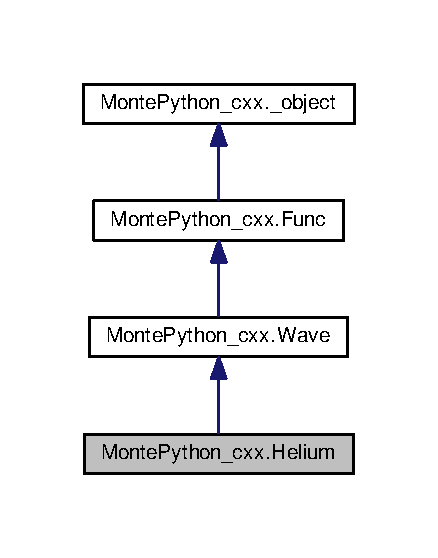
\includegraphics[width=210pt]{classMontePython__cxx_1_1Helium__inherit__graph}
\end{center}
\end{figure}


Collaboration diagram for Monte\+Python\+\_\+cxx.\+Helium\+:
\nopagebreak
\begin{figure}[H]
\begin{center}
\leavevmode
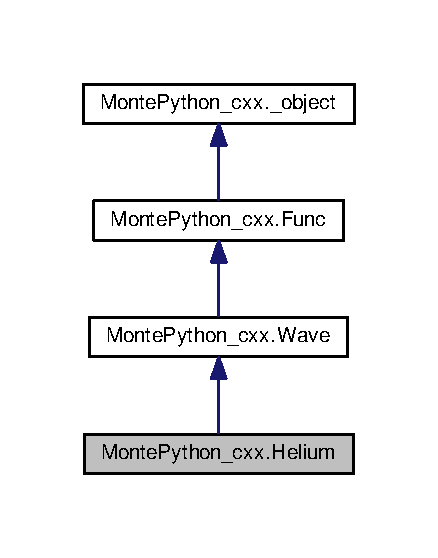
\includegraphics[width=210pt]{classMontePython__cxx_1_1Helium__coll__graph}
\end{center}
\end{figure}
\subsection*{Public Member Functions}
\begin{DoxyCompactItemize}
\item 
def \hyperlink{classMontePython__cxx_1_1Helium_a918ede66a3ed21e5ac82d22b9c668a0b}{set\+Params} (self, args)
\item 
def \hyperlink{classMontePython__cxx_1_1Helium_a730fee02af82ee1b0d274d2bf10c21d3}{value\+Pt} (self, args)
\item 
def \hyperlink{classMontePython__cxx_1_1Helium_ade191aeb115c184ff52373c87cdad9a5}{\+\_\+\+\_\+call\+\_\+\+\_\+} (self, args)
\item 
def \hyperlink{classMontePython__cxx_1_1Helium_aefabd0e6b5572a11ca43fde649caf01f}{\+\_\+\+\_\+init\+\_\+\+\_\+} (self)
\end{DoxyCompactItemize}
\subsection*{Public Attributes}
\begin{DoxyCompactItemize}
\item 
\hypertarget{classMontePython__cxx_1_1Helium_a3c63a6ac0ecf60dd4522dd9e5642b54b}{}{\bfseries this}\label{classMontePython__cxx_1_1Helium_a3c63a6ac0ecf60dd4522dd9e5642b54b}

\end{DoxyCompactItemize}
\subsection*{Static Private Attributes}
\begin{DoxyCompactItemize}
\item 
\hypertarget{classMontePython__cxx_1_1Helium_afb278ddd1dce33665736eced8590f138}{}dictionary {\bfseries \+\_\+\+\_\+swig\+\_\+setmethods\+\_\+\+\_\+} = \{\}\label{classMontePython__cxx_1_1Helium_afb278ddd1dce33665736eced8590f138}

\item 
\hypertarget{classMontePython__cxx_1_1Helium_ae13a338690d05160edd6f9d95c4b1e2b}{}tuple {\bfseries \+\_\+\+\_\+setattr\+\_\+\+\_\+} = lambdaself,name,value\+:\+\_\+swig\+\_\+setattr(self, \hyperlink{classMontePython__cxx_1_1Helium}{Helium}, name, value)\label{classMontePython__cxx_1_1Helium_ae13a338690d05160edd6f9d95c4b1e2b}

\item 
\hypertarget{classMontePython__cxx_1_1Helium_a40be2408a68b3d011eb950711631edcc}{}dictionary {\bfseries \+\_\+\+\_\+swig\+\_\+getmethods\+\_\+\+\_\+} = \{\}\label{classMontePython__cxx_1_1Helium_a40be2408a68b3d011eb950711631edcc}

\item 
\hypertarget{classMontePython__cxx_1_1Helium_ae3eb7437e193aaccd339e4dfb33fffc9}{}tuple {\bfseries \+\_\+\+\_\+getattr\+\_\+\+\_\+} = lambdaself,name\+:\+\_\+swig\+\_\+getattr(self, \hyperlink{classMontePython__cxx_1_1Helium}{Helium}, name)\label{classMontePython__cxx_1_1Helium_ae3eb7437e193aaccd339e4dfb33fffc9}

\item 
\hypertarget{classMontePython__cxx_1_1Helium_aa22251123c99ef6818adabcf96876111}{}{\bfseries \+\_\+\+\_\+repr\+\_\+\+\_\+} = \+\_\+swig\+\_\+repr\label{classMontePython__cxx_1_1Helium_aa22251123c99ef6818adabcf96876111}

\item 
\hypertarget{classMontePython__cxx_1_1Helium_a7a784f5221071761827dec2b910e0163}{}{\bfseries \+\_\+\+\_\+swig\+\_\+destroy\+\_\+\+\_\+} = \+\_\+\+Monte\+Python\+\_\+cxx.\+delete\+\_\+\+Helium\label{classMontePython__cxx_1_1Helium_a7a784f5221071761827dec2b910e0163}

\end{DoxyCompactItemize}


\subsection{Detailed Description}
\begin{DoxyVerb}Proxy of C++ Helium class\end{DoxyVerb}
 

\subsection{Constructor \& Destructor Documentation}
\hypertarget{classMontePython__cxx_1_1Helium_aefabd0e6b5572a11ca43fde649caf01f}{}\index{Monte\+Python\+\_\+cxx\+::\+Helium@{Monte\+Python\+\_\+cxx\+::\+Helium}!\+\_\+\+\_\+init\+\_\+\+\_\+@{\+\_\+\+\_\+init\+\_\+\+\_\+}}
\index{\+\_\+\+\_\+init\+\_\+\+\_\+@{\+\_\+\+\_\+init\+\_\+\+\_\+}!Monte\+Python\+\_\+cxx\+::\+Helium@{Monte\+Python\+\_\+cxx\+::\+Helium}}
\subsubsection[{\+\_\+\+\_\+init\+\_\+\+\_\+}]{\setlength{\rightskip}{0pt plus 5cm}def Monte\+Python\+\_\+cxx.\+Helium.\+\_\+\+\_\+init\+\_\+\+\_\+ (
\begin{DoxyParamCaption}
\item[{}]{self}
\end{DoxyParamCaption}
)}\label{classMontePython__cxx_1_1Helium_aefabd0e6b5572a11ca43fde649caf01f}
\begin{DoxyVerb}__init__(Helium self) -> Helium\end{DoxyVerb}
 

\subsection{Member Function Documentation}
\hypertarget{classMontePython__cxx_1_1Helium_ade191aeb115c184ff52373c87cdad9a5}{}\index{Monte\+Python\+\_\+cxx\+::\+Helium@{Monte\+Python\+\_\+cxx\+::\+Helium}!\+\_\+\+\_\+call\+\_\+\+\_\+@{\+\_\+\+\_\+call\+\_\+\+\_\+}}
\index{\+\_\+\+\_\+call\+\_\+\+\_\+@{\+\_\+\+\_\+call\+\_\+\+\_\+}!Monte\+Python\+\_\+cxx\+::\+Helium@{Monte\+Python\+\_\+cxx\+::\+Helium}}
\subsubsection[{\+\_\+\+\_\+call\+\_\+\+\_\+}]{\setlength{\rightskip}{0pt plus 5cm}def Monte\+Python\+\_\+cxx.\+Helium.\+\_\+\+\_\+call\+\_\+\+\_\+ (
\begin{DoxyParamCaption}
\item[{}]{self, }
\item[{}]{args}
\end{DoxyParamCaption}
)}\label{classMontePython__cxx_1_1Helium_ade191aeb115c184ff52373c87cdad9a5}
\begin{DoxyVerb}__call__(Helium self, QickArray & pos) -> double\end{DoxyVerb}
 \hypertarget{classMontePython__cxx_1_1Helium_a918ede66a3ed21e5ac82d22b9c668a0b}{}\index{Monte\+Python\+\_\+cxx\+::\+Helium@{Monte\+Python\+\_\+cxx\+::\+Helium}!set\+Params@{set\+Params}}
\index{set\+Params@{set\+Params}!Monte\+Python\+\_\+cxx\+::\+Helium@{Monte\+Python\+\_\+cxx\+::\+Helium}}
\subsubsection[{set\+Params}]{\setlength{\rightskip}{0pt plus 5cm}def Monte\+Python\+\_\+cxx.\+Helium.\+set\+Params (
\begin{DoxyParamCaption}
\item[{}]{self, }
\item[{}]{args}
\end{DoxyParamCaption}
)}\label{classMontePython__cxx_1_1Helium_a918ede66a3ed21e5ac82d22b9c668a0b}
\begin{DoxyVerb}setParams(Helium self, QickArray & params_)\end{DoxyVerb}
 \hypertarget{classMontePython__cxx_1_1Helium_a730fee02af82ee1b0d274d2bf10c21d3}{}\index{Monte\+Python\+\_\+cxx\+::\+Helium@{Monte\+Python\+\_\+cxx\+::\+Helium}!value\+Pt@{value\+Pt}}
\index{value\+Pt@{value\+Pt}!Monte\+Python\+\_\+cxx\+::\+Helium@{Monte\+Python\+\_\+cxx\+::\+Helium}}
\subsubsection[{value\+Pt}]{\setlength{\rightskip}{0pt plus 5cm}def Monte\+Python\+\_\+cxx.\+Helium.\+value\+Pt (
\begin{DoxyParamCaption}
\item[{}]{self, }
\item[{}]{args}
\end{DoxyParamCaption}
)}\label{classMontePython__cxx_1_1Helium_a730fee02af82ee1b0d274d2bf10c21d3}
\begin{DoxyVerb}valuePt(Helium self, QickArray & pos) -> double\end{DoxyVerb}
 

The documentation for this class was generated from the following file\+:\begin{DoxyCompactItemize}
\item 
Monte\+Python\+\_\+cxx.\+py\end{DoxyCompactItemize}

\hypertarget{classMontePython__cxx_1_1LiqHe4LocalEnergy}{}\section{Monte\+Python\+\_\+cxx.\+Liq\+He4\+Local\+Energy Class Reference}
\label{classMontePython__cxx_1_1LiqHe4LocalEnergy}\index{Monte\+Python\+\_\+cxx.\+Liq\+He4\+Local\+Energy@{Monte\+Python\+\_\+cxx.\+Liq\+He4\+Local\+Energy}}


Inheritance diagram for Monte\+Python\+\_\+cxx.\+Liq\+He4\+Local\+Energy\+:
\nopagebreak
\begin{figure}[H]
\begin{center}
\leavevmode
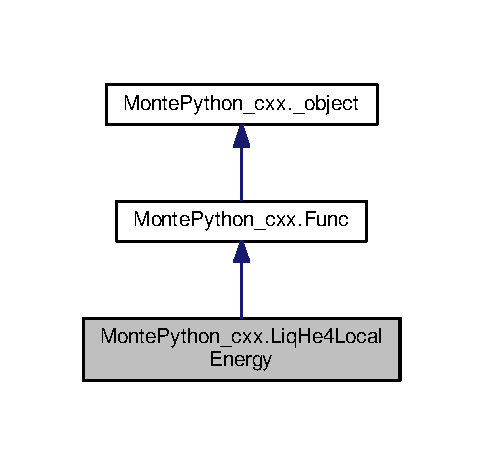
\includegraphics[width=232pt]{classMontePython__cxx_1_1LiqHe4LocalEnergy__inherit__graph}
\end{center}
\end{figure}


Collaboration diagram for Monte\+Python\+\_\+cxx.\+Liq\+He4\+Local\+Energy\+:
\nopagebreak
\begin{figure}[H]
\begin{center}
\leavevmode
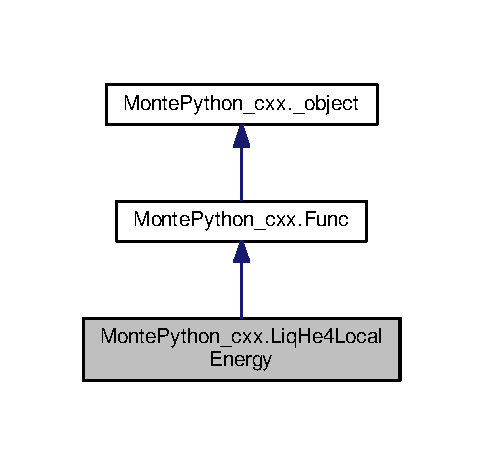
\includegraphics[width=232pt]{classMontePython__cxx_1_1LiqHe4LocalEnergy__coll__graph}
\end{center}
\end{figure}
\subsection*{Public Member Functions}
\begin{DoxyCompactItemize}
\item 
def \hyperlink{classMontePython__cxx_1_1LiqHe4LocalEnergy_ad230937699925551fde087370a5308b2}{set\+Params} (self, args)
\item 
def \hyperlink{classMontePython__cxx_1_1LiqHe4LocalEnergy_a358c425b9cec8651362981b5f70dc3ea}{value\+Pt} (self, args)
\item 
def \hyperlink{classMontePython__cxx_1_1LiqHe4LocalEnergy_a7c1ed8df2f49e4fafa753df731b7179d}{\+\_\+\+\_\+call\+\_\+\+\_\+} (self, args)
\item 
def \hyperlink{classMontePython__cxx_1_1LiqHe4LocalEnergy_a3107891e941cadedf20af4138fd88ea7}{\+\_\+\+\_\+init\+\_\+\+\_\+} (self)
\end{DoxyCompactItemize}
\subsection*{Public Attributes}
\begin{DoxyCompactItemize}
\item 
\hypertarget{classMontePython__cxx_1_1LiqHe4LocalEnergy_a01f035ffb57fb1090b94e9317540c914}{}{\bfseries this}\label{classMontePython__cxx_1_1LiqHe4LocalEnergy_a01f035ffb57fb1090b94e9317540c914}

\end{DoxyCompactItemize}
\subsection*{Static Private Attributes}
\begin{DoxyCompactItemize}
\item 
\hypertarget{classMontePython__cxx_1_1LiqHe4LocalEnergy_a29a3839abb7b7cff3ad52bb3f2b26aa2}{}dictionary {\bfseries \+\_\+\+\_\+swig\+\_\+setmethods\+\_\+\+\_\+} = \{\}\label{classMontePython__cxx_1_1LiqHe4LocalEnergy_a29a3839abb7b7cff3ad52bb3f2b26aa2}

\item 
\hypertarget{classMontePython__cxx_1_1LiqHe4LocalEnergy_a385e831ddfc46d1fbab59eaa501e440a}{}tuple {\bfseries \+\_\+\+\_\+setattr\+\_\+\+\_\+} = lambdaself,name,value\+:\+\_\+swig\+\_\+setattr(self, \hyperlink{classMontePython__cxx_1_1LiqHe4LocalEnergy}{Liq\+He4\+Local\+Energy}, name, value)\label{classMontePython__cxx_1_1LiqHe4LocalEnergy_a385e831ddfc46d1fbab59eaa501e440a}

\item 
\hypertarget{classMontePython__cxx_1_1LiqHe4LocalEnergy_ae9e91890c6a6b360271932fedc95d513}{}dictionary {\bfseries \+\_\+\+\_\+swig\+\_\+getmethods\+\_\+\+\_\+} = \{\}\label{classMontePython__cxx_1_1LiqHe4LocalEnergy_ae9e91890c6a6b360271932fedc95d513}

\item 
\hypertarget{classMontePython__cxx_1_1LiqHe4LocalEnergy_ad371960d2e8ada0536f73448a33e026a}{}tuple {\bfseries \+\_\+\+\_\+getattr\+\_\+\+\_\+} = lambdaself,name\+:\+\_\+swig\+\_\+getattr(self, \hyperlink{classMontePython__cxx_1_1LiqHe4LocalEnergy}{Liq\+He4\+Local\+Energy}, name)\label{classMontePython__cxx_1_1LiqHe4LocalEnergy_ad371960d2e8ada0536f73448a33e026a}

\item 
\hypertarget{classMontePython__cxx_1_1LiqHe4LocalEnergy_a25bc6174136c0301f85e9faacd13f780}{}{\bfseries \+\_\+\+\_\+repr\+\_\+\+\_\+} = \+\_\+swig\+\_\+repr\label{classMontePython__cxx_1_1LiqHe4LocalEnergy_a25bc6174136c0301f85e9faacd13f780}

\item 
\hypertarget{classMontePython__cxx_1_1LiqHe4LocalEnergy_afa92bd3be5bc92a58d9b674ecbe91583}{}{\bfseries \+\_\+\+\_\+swig\+\_\+destroy\+\_\+\+\_\+} = \+\_\+\+Monte\+Python\+\_\+cxx.\+delete\+\_\+\+Liq\+He4\+Local\+Energy\label{classMontePython__cxx_1_1LiqHe4LocalEnergy_afa92bd3be5bc92a58d9b674ecbe91583}

\end{DoxyCompactItemize}


\subsection{Detailed Description}
\begin{DoxyVerb}Proxy of C++ LiqHe4LocalEnergy class\end{DoxyVerb}
 

\subsection{Constructor \& Destructor Documentation}
\hypertarget{classMontePython__cxx_1_1LiqHe4LocalEnergy_a3107891e941cadedf20af4138fd88ea7}{}\index{Monte\+Python\+\_\+cxx\+::\+Liq\+He4\+Local\+Energy@{Monte\+Python\+\_\+cxx\+::\+Liq\+He4\+Local\+Energy}!\+\_\+\+\_\+init\+\_\+\+\_\+@{\+\_\+\+\_\+init\+\_\+\+\_\+}}
\index{\+\_\+\+\_\+init\+\_\+\+\_\+@{\+\_\+\+\_\+init\+\_\+\+\_\+}!Monte\+Python\+\_\+cxx\+::\+Liq\+He4\+Local\+Energy@{Monte\+Python\+\_\+cxx\+::\+Liq\+He4\+Local\+Energy}}
\subsubsection[{\+\_\+\+\_\+init\+\_\+\+\_\+}]{\setlength{\rightskip}{0pt plus 5cm}def Monte\+Python\+\_\+cxx.\+Liq\+He4\+Local\+Energy.\+\_\+\+\_\+init\+\_\+\+\_\+ (
\begin{DoxyParamCaption}
\item[{}]{self}
\end{DoxyParamCaption}
)}\label{classMontePython__cxx_1_1LiqHe4LocalEnergy_a3107891e941cadedf20af4138fd88ea7}
\begin{DoxyVerb}__init__(LiqHe4LocalEnergy self) -> LiqHe4LocalEnergy\end{DoxyVerb}
 

\subsection{Member Function Documentation}
\hypertarget{classMontePython__cxx_1_1LiqHe4LocalEnergy_a7c1ed8df2f49e4fafa753df731b7179d}{}\index{Monte\+Python\+\_\+cxx\+::\+Liq\+He4\+Local\+Energy@{Monte\+Python\+\_\+cxx\+::\+Liq\+He4\+Local\+Energy}!\+\_\+\+\_\+call\+\_\+\+\_\+@{\+\_\+\+\_\+call\+\_\+\+\_\+}}
\index{\+\_\+\+\_\+call\+\_\+\+\_\+@{\+\_\+\+\_\+call\+\_\+\+\_\+}!Monte\+Python\+\_\+cxx\+::\+Liq\+He4\+Local\+Energy@{Monte\+Python\+\_\+cxx\+::\+Liq\+He4\+Local\+Energy}}
\subsubsection[{\+\_\+\+\_\+call\+\_\+\+\_\+}]{\setlength{\rightskip}{0pt plus 5cm}def Monte\+Python\+\_\+cxx.\+Liq\+He4\+Local\+Energy.\+\_\+\+\_\+call\+\_\+\+\_\+ (
\begin{DoxyParamCaption}
\item[{}]{self, }
\item[{}]{args}
\end{DoxyParamCaption}
)}\label{classMontePython__cxx_1_1LiqHe4LocalEnergy_a7c1ed8df2f49e4fafa753df731b7179d}
\begin{DoxyVerb}__call__(LiqHe4LocalEnergy self, QickArray & pos) -> double\end{DoxyVerb}
 \hypertarget{classMontePython__cxx_1_1LiqHe4LocalEnergy_ad230937699925551fde087370a5308b2}{}\index{Monte\+Python\+\_\+cxx\+::\+Liq\+He4\+Local\+Energy@{Monte\+Python\+\_\+cxx\+::\+Liq\+He4\+Local\+Energy}!set\+Params@{set\+Params}}
\index{set\+Params@{set\+Params}!Monte\+Python\+\_\+cxx\+::\+Liq\+He4\+Local\+Energy@{Monte\+Python\+\_\+cxx\+::\+Liq\+He4\+Local\+Energy}}
\subsubsection[{set\+Params}]{\setlength{\rightskip}{0pt plus 5cm}def Monte\+Python\+\_\+cxx.\+Liq\+He4\+Local\+Energy.\+set\+Params (
\begin{DoxyParamCaption}
\item[{}]{self, }
\item[{}]{args}
\end{DoxyParamCaption}
)}\label{classMontePython__cxx_1_1LiqHe4LocalEnergy_ad230937699925551fde087370a5308b2}
\begin{DoxyVerb}setParams(LiqHe4LocalEnergy self, QickArray & params_)\end{DoxyVerb}
 \hypertarget{classMontePython__cxx_1_1LiqHe4LocalEnergy_a358c425b9cec8651362981b5f70dc3ea}{}\index{Monte\+Python\+\_\+cxx\+::\+Liq\+He4\+Local\+Energy@{Monte\+Python\+\_\+cxx\+::\+Liq\+He4\+Local\+Energy}!value\+Pt@{value\+Pt}}
\index{value\+Pt@{value\+Pt}!Monte\+Python\+\_\+cxx\+::\+Liq\+He4\+Local\+Energy@{Monte\+Python\+\_\+cxx\+::\+Liq\+He4\+Local\+Energy}}
\subsubsection[{value\+Pt}]{\setlength{\rightskip}{0pt plus 5cm}def Monte\+Python\+\_\+cxx.\+Liq\+He4\+Local\+Energy.\+value\+Pt (
\begin{DoxyParamCaption}
\item[{}]{self, }
\item[{}]{args}
\end{DoxyParamCaption}
)}\label{classMontePython__cxx_1_1LiqHe4LocalEnergy_a358c425b9cec8651362981b5f70dc3ea}
\begin{DoxyVerb}valuePt(LiqHe4LocalEnergy self, QickArray & pos) -> double\end{DoxyVerb}
 

The documentation for this class was generated from the following file\+:\begin{DoxyCompactItemize}
\item 
Monte\+Python\+\_\+cxx.\+py\end{DoxyCompactItemize}

\hypertarget{classMontePython__cxx_1_1LiqHe4QForce}{}\section{Monte\+Python\+\_\+cxx.\+Liq\+He4\+Q\+Force Class Reference}
\label{classMontePython__cxx_1_1LiqHe4QForce}\index{Monte\+Python\+\_\+cxx.\+Liq\+He4\+Q\+Force@{Monte\+Python\+\_\+cxx.\+Liq\+He4\+Q\+Force}}


Inheritance diagram for Monte\+Python\+\_\+cxx.\+Liq\+He4\+Q\+Force\+:
\nopagebreak
\begin{figure}[H]
\begin{center}
\leavevmode
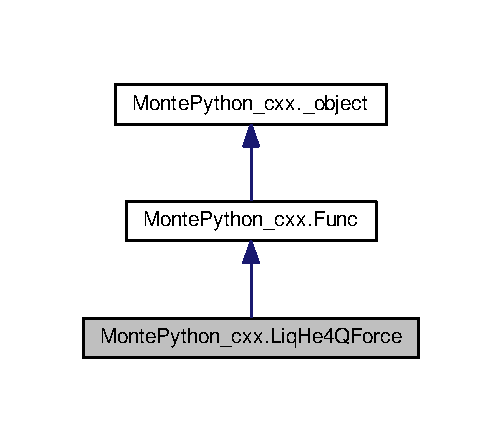
\includegraphics[width=241pt]{classMontePython__cxx_1_1LiqHe4QForce__inherit__graph}
\end{center}
\end{figure}


Collaboration diagram for Monte\+Python\+\_\+cxx.\+Liq\+He4\+Q\+Force\+:
\nopagebreak
\begin{figure}[H]
\begin{center}
\leavevmode
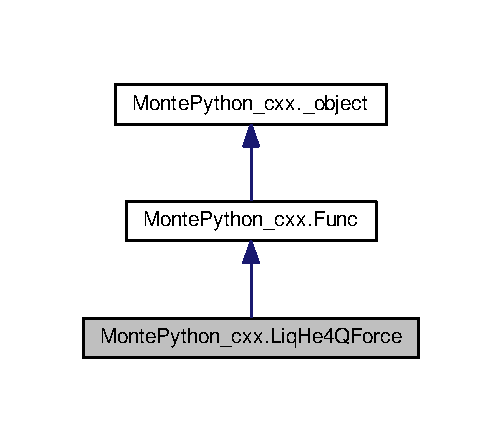
\includegraphics[width=241pt]{classMontePython__cxx_1_1LiqHe4QForce__coll__graph}
\end{center}
\end{figure}
\subsection*{Public Member Functions}
\begin{DoxyCompactItemize}
\item 
def \hyperlink{classMontePython__cxx_1_1LiqHe4QForce_aceae0c589524b9fd5cd8e12ee67b1227}{set\+Params} (self, args)
\item 
def \hyperlink{classMontePython__cxx_1_1LiqHe4QForce_a64134211ea9e7d6452bbdcc5ebc8d048}{value\+Pt} (self, args)
\item 
def \hyperlink{classMontePython__cxx_1_1LiqHe4QForce_aba75030eb38b62a6d672421abfc2b105}{\+\_\+\+\_\+call\+\_\+\+\_\+} (self, args)
\item 
def \hyperlink{classMontePython__cxx_1_1LiqHe4QForce_a5161efbae4eebf692f6dbdf295cac0a3}{\+\_\+\+\_\+init\+\_\+\+\_\+} (self)
\end{DoxyCompactItemize}
\subsection*{Public Attributes}
\begin{DoxyCompactItemize}
\item 
\hypertarget{classMontePython__cxx_1_1LiqHe4QForce_ae1410a74b2cdf5b87dc83c3f746593e9}{}{\bfseries this}\label{classMontePython__cxx_1_1LiqHe4QForce_ae1410a74b2cdf5b87dc83c3f746593e9}

\end{DoxyCompactItemize}
\subsection*{Static Private Attributes}
\begin{DoxyCompactItemize}
\item 
\hypertarget{classMontePython__cxx_1_1LiqHe4QForce_a439844b84804e3e711524a2a61577b99}{}dictionary {\bfseries \+\_\+\+\_\+swig\+\_\+setmethods\+\_\+\+\_\+} = \{\}\label{classMontePython__cxx_1_1LiqHe4QForce_a439844b84804e3e711524a2a61577b99}

\item 
\hypertarget{classMontePython__cxx_1_1LiqHe4QForce_ab3e449d56948fbad2b017002a9fbb435}{}tuple {\bfseries \+\_\+\+\_\+setattr\+\_\+\+\_\+} = lambdaself,name,value\+:\+\_\+swig\+\_\+setattr(self, \hyperlink{classMontePython__cxx_1_1LiqHe4QForce}{Liq\+He4\+Q\+Force}, name, value)\label{classMontePython__cxx_1_1LiqHe4QForce_ab3e449d56948fbad2b017002a9fbb435}

\item 
\hypertarget{classMontePython__cxx_1_1LiqHe4QForce_a119d3f8e1f8dbd8377fdcbea800c7576}{}dictionary {\bfseries \+\_\+\+\_\+swig\+\_\+getmethods\+\_\+\+\_\+} = \{\}\label{classMontePython__cxx_1_1LiqHe4QForce_a119d3f8e1f8dbd8377fdcbea800c7576}

\item 
\hypertarget{classMontePython__cxx_1_1LiqHe4QForce_ab1d6f91bd207b303dc323001a6dd383f}{}tuple {\bfseries \+\_\+\+\_\+getattr\+\_\+\+\_\+} = lambdaself,name\+:\+\_\+swig\+\_\+getattr(self, \hyperlink{classMontePython__cxx_1_1LiqHe4QForce}{Liq\+He4\+Q\+Force}, name)\label{classMontePython__cxx_1_1LiqHe4QForce_ab1d6f91bd207b303dc323001a6dd383f}

\item 
\hypertarget{classMontePython__cxx_1_1LiqHe4QForce_a734e59fdd57e7d74a7f0eee7061d94a5}{}{\bfseries \+\_\+\+\_\+repr\+\_\+\+\_\+} = \+\_\+swig\+\_\+repr\label{classMontePython__cxx_1_1LiqHe4QForce_a734e59fdd57e7d74a7f0eee7061d94a5}

\item 
\hypertarget{classMontePython__cxx_1_1LiqHe4QForce_a30beecd7d7bbb98fcdebcd78e2dd58d3}{}{\bfseries \+\_\+\+\_\+swig\+\_\+destroy\+\_\+\+\_\+} = \+\_\+\+Monte\+Python\+\_\+cxx.\+delete\+\_\+\+Liq\+He4\+Q\+Force\label{classMontePython__cxx_1_1LiqHe4QForce_a30beecd7d7bbb98fcdebcd78e2dd58d3}

\end{DoxyCompactItemize}


\subsection{Detailed Description}
\begin{DoxyVerb}Proxy of C++ LiqHe4QForce class\end{DoxyVerb}
 

\subsection{Constructor \& Destructor Documentation}
\hypertarget{classMontePython__cxx_1_1LiqHe4QForce_a5161efbae4eebf692f6dbdf295cac0a3}{}\index{Monte\+Python\+\_\+cxx\+::\+Liq\+He4\+Q\+Force@{Monte\+Python\+\_\+cxx\+::\+Liq\+He4\+Q\+Force}!\+\_\+\+\_\+init\+\_\+\+\_\+@{\+\_\+\+\_\+init\+\_\+\+\_\+}}
\index{\+\_\+\+\_\+init\+\_\+\+\_\+@{\+\_\+\+\_\+init\+\_\+\+\_\+}!Monte\+Python\+\_\+cxx\+::\+Liq\+He4\+Q\+Force@{Monte\+Python\+\_\+cxx\+::\+Liq\+He4\+Q\+Force}}
\subsubsection[{\+\_\+\+\_\+init\+\_\+\+\_\+}]{\setlength{\rightskip}{0pt plus 5cm}def Monte\+Python\+\_\+cxx.\+Liq\+He4\+Q\+Force.\+\_\+\+\_\+init\+\_\+\+\_\+ (
\begin{DoxyParamCaption}
\item[{}]{self}
\end{DoxyParamCaption}
)}\label{classMontePython__cxx_1_1LiqHe4QForce_a5161efbae4eebf692f6dbdf295cac0a3}
\begin{DoxyVerb}__init__(LiqHe4QForce self) -> LiqHe4QForce\end{DoxyVerb}
 

\subsection{Member Function Documentation}
\hypertarget{classMontePython__cxx_1_1LiqHe4QForce_aba75030eb38b62a6d672421abfc2b105}{}\index{Monte\+Python\+\_\+cxx\+::\+Liq\+He4\+Q\+Force@{Monte\+Python\+\_\+cxx\+::\+Liq\+He4\+Q\+Force}!\+\_\+\+\_\+call\+\_\+\+\_\+@{\+\_\+\+\_\+call\+\_\+\+\_\+}}
\index{\+\_\+\+\_\+call\+\_\+\+\_\+@{\+\_\+\+\_\+call\+\_\+\+\_\+}!Monte\+Python\+\_\+cxx\+::\+Liq\+He4\+Q\+Force@{Monte\+Python\+\_\+cxx\+::\+Liq\+He4\+Q\+Force}}
\subsubsection[{\+\_\+\+\_\+call\+\_\+\+\_\+}]{\setlength{\rightskip}{0pt plus 5cm}def Monte\+Python\+\_\+cxx.\+Liq\+He4\+Q\+Force.\+\_\+\+\_\+call\+\_\+\+\_\+ (
\begin{DoxyParamCaption}
\item[{}]{self, }
\item[{}]{args}
\end{DoxyParamCaption}
)}\label{classMontePython__cxx_1_1LiqHe4QForce_aba75030eb38b62a6d672421abfc2b105}
\begin{DoxyVerb}__call__(LiqHe4QForce self, QickArray & pos, bool dummy) -> QickArray &\end{DoxyVerb}
 \hypertarget{classMontePython__cxx_1_1LiqHe4QForce_aceae0c589524b9fd5cd8e12ee67b1227}{}\index{Monte\+Python\+\_\+cxx\+::\+Liq\+He4\+Q\+Force@{Monte\+Python\+\_\+cxx\+::\+Liq\+He4\+Q\+Force}!set\+Params@{set\+Params}}
\index{set\+Params@{set\+Params}!Monte\+Python\+\_\+cxx\+::\+Liq\+He4\+Q\+Force@{Monte\+Python\+\_\+cxx\+::\+Liq\+He4\+Q\+Force}}
\subsubsection[{set\+Params}]{\setlength{\rightskip}{0pt plus 5cm}def Monte\+Python\+\_\+cxx.\+Liq\+He4\+Q\+Force.\+set\+Params (
\begin{DoxyParamCaption}
\item[{}]{self, }
\item[{}]{args}
\end{DoxyParamCaption}
)}\label{classMontePython__cxx_1_1LiqHe4QForce_aceae0c589524b9fd5cd8e12ee67b1227}
\begin{DoxyVerb}setParams(LiqHe4QForce self, QickArray & params_)\end{DoxyVerb}
 \hypertarget{classMontePython__cxx_1_1LiqHe4QForce_a64134211ea9e7d6452bbdcc5ebc8d048}{}\index{Monte\+Python\+\_\+cxx\+::\+Liq\+He4\+Q\+Force@{Monte\+Python\+\_\+cxx\+::\+Liq\+He4\+Q\+Force}!value\+Pt@{value\+Pt}}
\index{value\+Pt@{value\+Pt}!Monte\+Python\+\_\+cxx\+::\+Liq\+He4\+Q\+Force@{Monte\+Python\+\_\+cxx\+::\+Liq\+He4\+Q\+Force}}
\subsubsection[{value\+Pt}]{\setlength{\rightskip}{0pt plus 5cm}def Monte\+Python\+\_\+cxx.\+Liq\+He4\+Q\+Force.\+value\+Pt (
\begin{DoxyParamCaption}
\item[{}]{self, }
\item[{}]{args}
\end{DoxyParamCaption}
)}\label{classMontePython__cxx_1_1LiqHe4QForce_a64134211ea9e7d6452bbdcc5ebc8d048}
\begin{DoxyVerb}valuePt(LiqHe4QForce self, QickArray & pos, bool dummy) -> QickArray &\end{DoxyVerb}
 

The documentation for this class was generated from the following file\+:\begin{DoxyCompactItemize}
\item 
Monte\+Python\+\_\+cxx.\+py\end{DoxyCompactItemize}

\hypertarget{classMontePython__cxx_1_1LiqHe4QForceNum}{}\section{Monte\+Python\+\_\+cxx.\+Liq\+He4\+Q\+Force\+Num Class Reference}
\label{classMontePython__cxx_1_1LiqHe4QForceNum}\index{Monte\+Python\+\_\+cxx.\+Liq\+He4\+Q\+Force\+Num@{Monte\+Python\+\_\+cxx.\+Liq\+He4\+Q\+Force\+Num}}


Inheritance diagram for Monte\+Python\+\_\+cxx.\+Liq\+He4\+Q\+Force\+Num\+:
\nopagebreak
\begin{figure}[H]
\begin{center}
\leavevmode
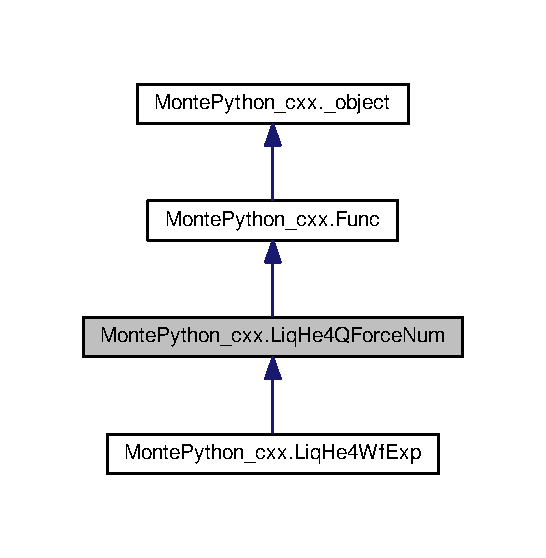
\includegraphics[width=262pt]{classMontePython__cxx_1_1LiqHe4QForceNum__inherit__graph}
\end{center}
\end{figure}


Collaboration diagram for Monte\+Python\+\_\+cxx.\+Liq\+He4\+Q\+Force\+Num\+:
\nopagebreak
\begin{figure}[H]
\begin{center}
\leavevmode
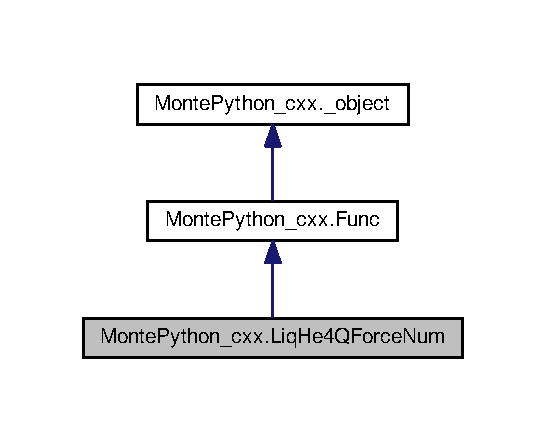
\includegraphics[width=262pt]{classMontePython__cxx_1_1LiqHe4QForceNum__coll__graph}
\end{center}
\end{figure}
\subsection*{Public Member Functions}
\begin{DoxyCompactItemize}
\item 
def \hyperlink{classMontePython__cxx_1_1LiqHe4QForceNum_a64c502cd19b8e65f5c9b5f4cddb41f60}{set\+Params} (self, args)
\item 
def \hyperlink{classMontePython__cxx_1_1LiqHe4QForceNum_a070425028c6c7c08e136fde84b00204f}{value\+Pt} (self, args)
\item 
def \hyperlink{classMontePython__cxx_1_1LiqHe4QForceNum_a1c7971c4fed28b2ce365ea75401420e5}{\+\_\+\+\_\+call\+\_\+\+\_\+} (self, args)
\item 
def \hyperlink{classMontePython__cxx_1_1LiqHe4QForceNum_ab9008bcb1b618c5ce8c2b3e257bedacf}{\+\_\+\+\_\+init\+\_\+\+\_\+} (self)
\end{DoxyCompactItemize}
\subsection*{Public Attributes}
\begin{DoxyCompactItemize}
\item 
\hypertarget{classMontePython__cxx_1_1LiqHe4QForceNum_a0950b6ec4fa8e7151674702255a5f021}{}{\bfseries this}\label{classMontePython__cxx_1_1LiqHe4QForceNum_a0950b6ec4fa8e7151674702255a5f021}

\end{DoxyCompactItemize}
\subsection*{Static Private Attributes}
\begin{DoxyCompactItemize}
\item 
\hypertarget{classMontePython__cxx_1_1LiqHe4QForceNum_a7c3e74b103d64ef8796cbda3d3f86fde}{}dictionary {\bfseries \+\_\+\+\_\+swig\+\_\+setmethods\+\_\+\+\_\+} = \{\}\label{classMontePython__cxx_1_1LiqHe4QForceNum_a7c3e74b103d64ef8796cbda3d3f86fde}

\item 
\hypertarget{classMontePython__cxx_1_1LiqHe4QForceNum_a5bf48893590dd2b90c3770271ec33f4d}{}tuple {\bfseries \+\_\+\+\_\+setattr\+\_\+\+\_\+} = lambdaself,name,value\+:\+\_\+swig\+\_\+setattr(self, \hyperlink{classMontePython__cxx_1_1LiqHe4QForceNum}{Liq\+He4\+Q\+Force\+Num}, name, value)\label{classMontePython__cxx_1_1LiqHe4QForceNum_a5bf48893590dd2b90c3770271ec33f4d}

\item 
\hypertarget{classMontePython__cxx_1_1LiqHe4QForceNum_af57fd2bdfeb3de46731c0299dc2db5ac}{}dictionary {\bfseries \+\_\+\+\_\+swig\+\_\+getmethods\+\_\+\+\_\+} = \{\}\label{classMontePython__cxx_1_1LiqHe4QForceNum_af57fd2bdfeb3de46731c0299dc2db5ac}

\item 
\hypertarget{classMontePython__cxx_1_1LiqHe4QForceNum_a5c654d8ee497ce330aa82d9f2058ee11}{}tuple {\bfseries \+\_\+\+\_\+getattr\+\_\+\+\_\+} = lambdaself,name\+:\+\_\+swig\+\_\+getattr(self, \hyperlink{classMontePython__cxx_1_1LiqHe4QForceNum}{Liq\+He4\+Q\+Force\+Num}, name)\label{classMontePython__cxx_1_1LiqHe4QForceNum_a5c654d8ee497ce330aa82d9f2058ee11}

\item 
\hypertarget{classMontePython__cxx_1_1LiqHe4QForceNum_a01508a5ffd2f4d0d4e35a9f923b2ef41}{}{\bfseries \+\_\+\+\_\+repr\+\_\+\+\_\+} = \+\_\+swig\+\_\+repr\label{classMontePython__cxx_1_1LiqHe4QForceNum_a01508a5ffd2f4d0d4e35a9f923b2ef41}

\item 
\hypertarget{classMontePython__cxx_1_1LiqHe4QForceNum_a0f049222801f5f320806afc3b96ed877}{}{\bfseries \+\_\+\+\_\+swig\+\_\+destroy\+\_\+\+\_\+} = \+\_\+\+Monte\+Python\+\_\+cxx.\+delete\+\_\+\+Liq\+He4\+Q\+Force\+Num\label{classMontePython__cxx_1_1LiqHe4QForceNum_a0f049222801f5f320806afc3b96ed877}

\end{DoxyCompactItemize}


\subsection{Detailed Description}
\begin{DoxyVerb}Proxy of C++ LiqHe4QForceNum class\end{DoxyVerb}
 

\subsection{Constructor \& Destructor Documentation}
\hypertarget{classMontePython__cxx_1_1LiqHe4QForceNum_ab9008bcb1b618c5ce8c2b3e257bedacf}{}\index{Monte\+Python\+\_\+cxx\+::\+Liq\+He4\+Q\+Force\+Num@{Monte\+Python\+\_\+cxx\+::\+Liq\+He4\+Q\+Force\+Num}!\+\_\+\+\_\+init\+\_\+\+\_\+@{\+\_\+\+\_\+init\+\_\+\+\_\+}}
\index{\+\_\+\+\_\+init\+\_\+\+\_\+@{\+\_\+\+\_\+init\+\_\+\+\_\+}!Monte\+Python\+\_\+cxx\+::\+Liq\+He4\+Q\+Force\+Num@{Monte\+Python\+\_\+cxx\+::\+Liq\+He4\+Q\+Force\+Num}}
\subsubsection[{\+\_\+\+\_\+init\+\_\+\+\_\+}]{\setlength{\rightskip}{0pt plus 5cm}def Monte\+Python\+\_\+cxx.\+Liq\+He4\+Q\+Force\+Num.\+\_\+\+\_\+init\+\_\+\+\_\+ (
\begin{DoxyParamCaption}
\item[{}]{self}
\end{DoxyParamCaption}
)}\label{classMontePython__cxx_1_1LiqHe4QForceNum_ab9008bcb1b618c5ce8c2b3e257bedacf}
\begin{DoxyVerb}__init__(LiqHe4QForceNum self) -> LiqHe4QForceNum\end{DoxyVerb}
 

\subsection{Member Function Documentation}
\hypertarget{classMontePython__cxx_1_1LiqHe4QForceNum_a1c7971c4fed28b2ce365ea75401420e5}{}\index{Monte\+Python\+\_\+cxx\+::\+Liq\+He4\+Q\+Force\+Num@{Monte\+Python\+\_\+cxx\+::\+Liq\+He4\+Q\+Force\+Num}!\+\_\+\+\_\+call\+\_\+\+\_\+@{\+\_\+\+\_\+call\+\_\+\+\_\+}}
\index{\+\_\+\+\_\+call\+\_\+\+\_\+@{\+\_\+\+\_\+call\+\_\+\+\_\+}!Monte\+Python\+\_\+cxx\+::\+Liq\+He4\+Q\+Force\+Num@{Monte\+Python\+\_\+cxx\+::\+Liq\+He4\+Q\+Force\+Num}}
\subsubsection[{\+\_\+\+\_\+call\+\_\+\+\_\+}]{\setlength{\rightskip}{0pt plus 5cm}def Monte\+Python\+\_\+cxx.\+Liq\+He4\+Q\+Force\+Num.\+\_\+\+\_\+call\+\_\+\+\_\+ (
\begin{DoxyParamCaption}
\item[{}]{self, }
\item[{}]{args}
\end{DoxyParamCaption}
)}\label{classMontePython__cxx_1_1LiqHe4QForceNum_a1c7971c4fed28b2ce365ea75401420e5}
\begin{DoxyVerb}__call__(LiqHe4QForceNum self, QickArray & pos, bool dummy) -> QickArray &\end{DoxyVerb}
 \hypertarget{classMontePython__cxx_1_1LiqHe4QForceNum_a64c502cd19b8e65f5c9b5f4cddb41f60}{}\index{Monte\+Python\+\_\+cxx\+::\+Liq\+He4\+Q\+Force\+Num@{Monte\+Python\+\_\+cxx\+::\+Liq\+He4\+Q\+Force\+Num}!set\+Params@{set\+Params}}
\index{set\+Params@{set\+Params}!Monte\+Python\+\_\+cxx\+::\+Liq\+He4\+Q\+Force\+Num@{Monte\+Python\+\_\+cxx\+::\+Liq\+He4\+Q\+Force\+Num}}
\subsubsection[{set\+Params}]{\setlength{\rightskip}{0pt plus 5cm}def Monte\+Python\+\_\+cxx.\+Liq\+He4\+Q\+Force\+Num.\+set\+Params (
\begin{DoxyParamCaption}
\item[{}]{self, }
\item[{}]{args}
\end{DoxyParamCaption}
)}\label{classMontePython__cxx_1_1LiqHe4QForceNum_a64c502cd19b8e65f5c9b5f4cddb41f60}
\begin{DoxyVerb}setParams(LiqHe4QForceNum self, QickArray & params_)\end{DoxyVerb}
 \hypertarget{classMontePython__cxx_1_1LiqHe4QForceNum_a070425028c6c7c08e136fde84b00204f}{}\index{Monte\+Python\+\_\+cxx\+::\+Liq\+He4\+Q\+Force\+Num@{Monte\+Python\+\_\+cxx\+::\+Liq\+He4\+Q\+Force\+Num}!value\+Pt@{value\+Pt}}
\index{value\+Pt@{value\+Pt}!Monte\+Python\+\_\+cxx\+::\+Liq\+He4\+Q\+Force\+Num@{Monte\+Python\+\_\+cxx\+::\+Liq\+He4\+Q\+Force\+Num}}
\subsubsection[{value\+Pt}]{\setlength{\rightskip}{0pt plus 5cm}def Monte\+Python\+\_\+cxx.\+Liq\+He4\+Q\+Force\+Num.\+value\+Pt (
\begin{DoxyParamCaption}
\item[{}]{self, }
\item[{}]{args}
\end{DoxyParamCaption}
)}\label{classMontePython__cxx_1_1LiqHe4QForceNum_a070425028c6c7c08e136fde84b00204f}
\begin{DoxyVerb}valuePt(LiqHe4QForceNum self, QickArray & pos, bool dummy) -> QickArray &\end{DoxyVerb}
 

The documentation for this class was generated from the following file\+:\begin{DoxyCompactItemize}
\item 
Monte\+Python\+\_\+cxx.\+py\end{DoxyCompactItemize}

\hypertarget{classMontePython__cxx_1_1LiqHe4Wave}{}\section{Monte\+Python\+\_\+cxx.\+Liq\+He4\+Wave Class Reference}
\label{classMontePython__cxx_1_1LiqHe4Wave}\index{Monte\+Python\+\_\+cxx.\+Liq\+He4\+Wave@{Monte\+Python\+\_\+cxx.\+Liq\+He4\+Wave}}


Inheritance diagram for Monte\+Python\+\_\+cxx.\+Liq\+He4\+Wave\+:
\nopagebreak
\begin{figure}[H]
\begin{center}
\leavevmode
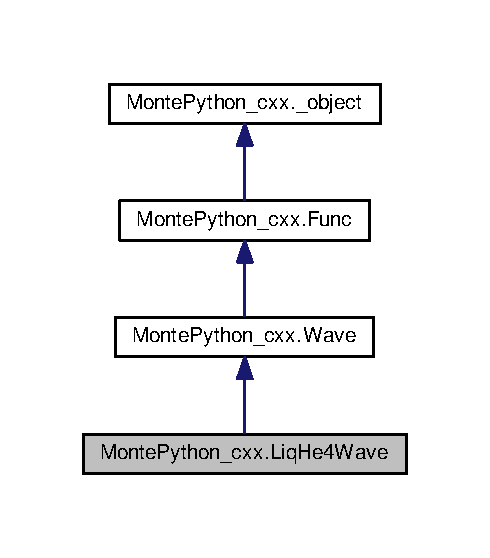
\includegraphics[width=235pt]{classMontePython__cxx_1_1LiqHe4Wave__inherit__graph}
\end{center}
\end{figure}


Collaboration diagram for Monte\+Python\+\_\+cxx.\+Liq\+He4\+Wave\+:
\nopagebreak
\begin{figure}[H]
\begin{center}
\leavevmode
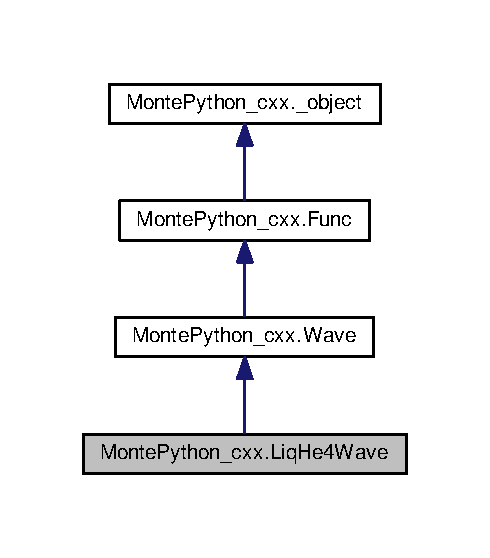
\includegraphics[width=235pt]{classMontePython__cxx_1_1LiqHe4Wave__coll__graph}
\end{center}
\end{figure}
\subsection*{Public Member Functions}
\begin{DoxyCompactItemize}
\item 
def \hyperlink{classMontePython__cxx_1_1LiqHe4Wave_a9fb7855179e1e1779e6f5e61aad94508}{set\+Params} (self, args)
\item 
def \hyperlink{classMontePython__cxx_1_1LiqHe4Wave_a4d943bc517c1a32cfdfe76748d6b087f}{value\+Pt} (self, args)
\item 
def \hyperlink{classMontePython__cxx_1_1LiqHe4Wave_a0604145deac62db776e907448e38adbf}{\+\_\+\+\_\+call\+\_\+\+\_\+} (self, args)
\item 
def \hyperlink{classMontePython__cxx_1_1LiqHe4Wave_a853439441228737bf2a2f6445c687163}{\+\_\+\+\_\+init\+\_\+\+\_\+} (self)
\end{DoxyCompactItemize}
\subsection*{Public Attributes}
\begin{DoxyCompactItemize}
\item 
\hypertarget{classMontePython__cxx_1_1LiqHe4Wave_a28c9beb4416f132efad1dc148c83ad70}{}{\bfseries this}\label{classMontePython__cxx_1_1LiqHe4Wave_a28c9beb4416f132efad1dc148c83ad70}

\end{DoxyCompactItemize}
\subsection*{Static Private Attributes}
\begin{DoxyCompactItemize}
\item 
\hypertarget{classMontePython__cxx_1_1LiqHe4Wave_a6da2f8692cf790b51aafb632d290c500}{}dictionary {\bfseries \+\_\+\+\_\+swig\+\_\+setmethods\+\_\+\+\_\+} = \{\}\label{classMontePython__cxx_1_1LiqHe4Wave_a6da2f8692cf790b51aafb632d290c500}

\item 
\hypertarget{classMontePython__cxx_1_1LiqHe4Wave_ac8493f76bf73f90143e3e6cc11b37dfa}{}tuple {\bfseries \+\_\+\+\_\+setattr\+\_\+\+\_\+} = lambdaself,name,value\+:\+\_\+swig\+\_\+setattr(self, \hyperlink{classMontePython__cxx_1_1LiqHe4Wave}{Liq\+He4\+Wave}, name, value)\label{classMontePython__cxx_1_1LiqHe4Wave_ac8493f76bf73f90143e3e6cc11b37dfa}

\item 
\hypertarget{classMontePython__cxx_1_1LiqHe4Wave_a3fd7cf3eda09f3687b48e7e6eca12edf}{}dictionary {\bfseries \+\_\+\+\_\+swig\+\_\+getmethods\+\_\+\+\_\+} = \{\}\label{classMontePython__cxx_1_1LiqHe4Wave_a3fd7cf3eda09f3687b48e7e6eca12edf}

\item 
\hypertarget{classMontePython__cxx_1_1LiqHe4Wave_a9dbda74c49a67a555ba83544ea83d4e1}{}tuple {\bfseries \+\_\+\+\_\+getattr\+\_\+\+\_\+} = lambdaself,name\+:\+\_\+swig\+\_\+getattr(self, \hyperlink{classMontePython__cxx_1_1LiqHe4Wave}{Liq\+He4\+Wave}, name)\label{classMontePython__cxx_1_1LiqHe4Wave_a9dbda74c49a67a555ba83544ea83d4e1}

\item 
\hypertarget{classMontePython__cxx_1_1LiqHe4Wave_aa83464e148a36eb95bd345e751c46677}{}{\bfseries \+\_\+\+\_\+repr\+\_\+\+\_\+} = \+\_\+swig\+\_\+repr\label{classMontePython__cxx_1_1LiqHe4Wave_aa83464e148a36eb95bd345e751c46677}

\item 
\hypertarget{classMontePython__cxx_1_1LiqHe4Wave_a7f6786a92722dbe26c9c35119939ef8b}{}{\bfseries \+\_\+\+\_\+swig\+\_\+destroy\+\_\+\+\_\+} = \+\_\+\+Monte\+Python\+\_\+cxx.\+delete\+\_\+\+Liq\+He4\+Wave\label{classMontePython__cxx_1_1LiqHe4Wave_a7f6786a92722dbe26c9c35119939ef8b}

\end{DoxyCompactItemize}


\subsection{Detailed Description}
\begin{DoxyVerb}Proxy of C++ LiqHe4Wave class\end{DoxyVerb}
 

\subsection{Constructor \& Destructor Documentation}
\hypertarget{classMontePython__cxx_1_1LiqHe4Wave_a853439441228737bf2a2f6445c687163}{}\index{Monte\+Python\+\_\+cxx\+::\+Liq\+He4\+Wave@{Monte\+Python\+\_\+cxx\+::\+Liq\+He4\+Wave}!\+\_\+\+\_\+init\+\_\+\+\_\+@{\+\_\+\+\_\+init\+\_\+\+\_\+}}
\index{\+\_\+\+\_\+init\+\_\+\+\_\+@{\+\_\+\+\_\+init\+\_\+\+\_\+}!Monte\+Python\+\_\+cxx\+::\+Liq\+He4\+Wave@{Monte\+Python\+\_\+cxx\+::\+Liq\+He4\+Wave}}
\subsubsection[{\+\_\+\+\_\+init\+\_\+\+\_\+}]{\setlength{\rightskip}{0pt plus 5cm}def Monte\+Python\+\_\+cxx.\+Liq\+He4\+Wave.\+\_\+\+\_\+init\+\_\+\+\_\+ (
\begin{DoxyParamCaption}
\item[{}]{self}
\end{DoxyParamCaption}
)}\label{classMontePython__cxx_1_1LiqHe4Wave_a853439441228737bf2a2f6445c687163}
\begin{DoxyVerb}__init__(LiqHe4Wave self) -> LiqHe4Wave\end{DoxyVerb}
 

\subsection{Member Function Documentation}
\hypertarget{classMontePython__cxx_1_1LiqHe4Wave_a0604145deac62db776e907448e38adbf}{}\index{Monte\+Python\+\_\+cxx\+::\+Liq\+He4\+Wave@{Monte\+Python\+\_\+cxx\+::\+Liq\+He4\+Wave}!\+\_\+\+\_\+call\+\_\+\+\_\+@{\+\_\+\+\_\+call\+\_\+\+\_\+}}
\index{\+\_\+\+\_\+call\+\_\+\+\_\+@{\+\_\+\+\_\+call\+\_\+\+\_\+}!Monte\+Python\+\_\+cxx\+::\+Liq\+He4\+Wave@{Monte\+Python\+\_\+cxx\+::\+Liq\+He4\+Wave}}
\subsubsection[{\+\_\+\+\_\+call\+\_\+\+\_\+}]{\setlength{\rightskip}{0pt plus 5cm}def Monte\+Python\+\_\+cxx.\+Liq\+He4\+Wave.\+\_\+\+\_\+call\+\_\+\+\_\+ (
\begin{DoxyParamCaption}
\item[{}]{self, }
\item[{}]{args}
\end{DoxyParamCaption}
)}\label{classMontePython__cxx_1_1LiqHe4Wave_a0604145deac62db776e907448e38adbf}
\begin{DoxyVerb}__call__(LiqHe4Wave self, QickArray & pos) -> double\end{DoxyVerb}
 \hypertarget{classMontePython__cxx_1_1LiqHe4Wave_a9fb7855179e1e1779e6f5e61aad94508}{}\index{Monte\+Python\+\_\+cxx\+::\+Liq\+He4\+Wave@{Monte\+Python\+\_\+cxx\+::\+Liq\+He4\+Wave}!set\+Params@{set\+Params}}
\index{set\+Params@{set\+Params}!Monte\+Python\+\_\+cxx\+::\+Liq\+He4\+Wave@{Monte\+Python\+\_\+cxx\+::\+Liq\+He4\+Wave}}
\subsubsection[{set\+Params}]{\setlength{\rightskip}{0pt plus 5cm}def Monte\+Python\+\_\+cxx.\+Liq\+He4\+Wave.\+set\+Params (
\begin{DoxyParamCaption}
\item[{}]{self, }
\item[{}]{args}
\end{DoxyParamCaption}
)}\label{classMontePython__cxx_1_1LiqHe4Wave_a9fb7855179e1e1779e6f5e61aad94508}
\begin{DoxyVerb}setParams(LiqHe4Wave self, QickArray & params_)\end{DoxyVerb}
 \hypertarget{classMontePython__cxx_1_1LiqHe4Wave_a4d943bc517c1a32cfdfe76748d6b087f}{}\index{Monte\+Python\+\_\+cxx\+::\+Liq\+He4\+Wave@{Monte\+Python\+\_\+cxx\+::\+Liq\+He4\+Wave}!value\+Pt@{value\+Pt}}
\index{value\+Pt@{value\+Pt}!Monte\+Python\+\_\+cxx\+::\+Liq\+He4\+Wave@{Monte\+Python\+\_\+cxx\+::\+Liq\+He4\+Wave}}
\subsubsection[{value\+Pt}]{\setlength{\rightskip}{0pt plus 5cm}def Monte\+Python\+\_\+cxx.\+Liq\+He4\+Wave.\+value\+Pt (
\begin{DoxyParamCaption}
\item[{}]{self, }
\item[{}]{args}
\end{DoxyParamCaption}
)}\label{classMontePython__cxx_1_1LiqHe4Wave_a4d943bc517c1a32cfdfe76748d6b087f}
\begin{DoxyVerb}valuePt(LiqHe4Wave self, QickArray & pos) -> double\end{DoxyVerb}
 

The documentation for this class was generated from the following file\+:\begin{DoxyCompactItemize}
\item 
Monte\+Python\+\_\+cxx.\+py\end{DoxyCompactItemize}

\hypertarget{classMontePython__cxx_1_1LiqHe4WaveAll}{}\section{Monte\+Python\+\_\+cxx.\+Liq\+He4\+Wave\+All Class Reference}
\label{classMontePython__cxx_1_1LiqHe4WaveAll}\index{Monte\+Python\+\_\+cxx.\+Liq\+He4\+Wave\+All@{Monte\+Python\+\_\+cxx.\+Liq\+He4\+Wave\+All}}


Inheritance diagram for Monte\+Python\+\_\+cxx.\+Liq\+He4\+Wave\+All\+:
\nopagebreak
\begin{figure}[H]
\begin{center}
\leavevmode
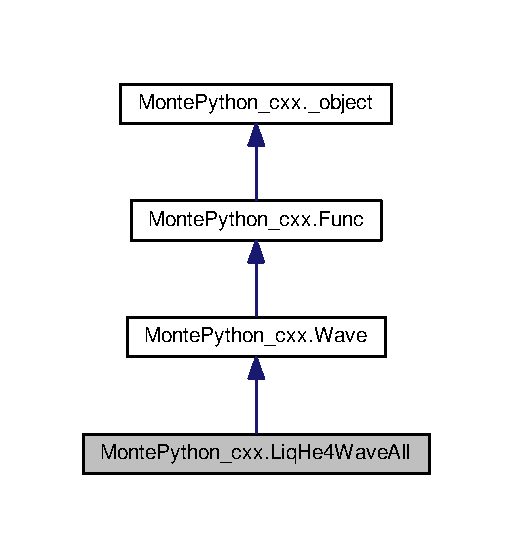
\includegraphics[width=246pt]{classMontePython__cxx_1_1LiqHe4WaveAll__inherit__graph}
\end{center}
\end{figure}


Collaboration diagram for Monte\+Python\+\_\+cxx.\+Liq\+He4\+Wave\+All\+:
\nopagebreak
\begin{figure}[H]
\begin{center}
\leavevmode
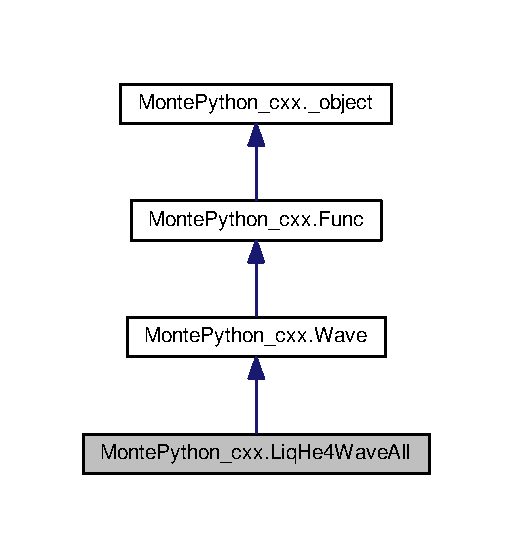
\includegraphics[width=246pt]{classMontePython__cxx_1_1LiqHe4WaveAll__coll__graph}
\end{center}
\end{figure}
\subsection*{Public Member Functions}
\begin{DoxyCompactItemize}
\item 
def \hyperlink{classMontePython__cxx_1_1LiqHe4WaveAll_af1ed254dfb18f5bdfa98e4e81ef45464}{set\+Params} (self, args)
\item 
def \hyperlink{classMontePython__cxx_1_1LiqHe4WaveAll_acebef3bf01d5285013473b0e43f3962c}{value\+Pt} (self, args)
\item 
def \hyperlink{classMontePython__cxx_1_1LiqHe4WaveAll_aa3d18ee6af9df1521846436c950e3cec}{\+\_\+\+\_\+call\+\_\+\+\_\+} (self, args)
\item 
def \hyperlink{classMontePython__cxx_1_1LiqHe4WaveAll_ae4d7cba00a8d1da0fc83595658e0d295}{\+\_\+\+\_\+init\+\_\+\+\_\+} (self)
\end{DoxyCompactItemize}
\subsection*{Public Attributes}
\begin{DoxyCompactItemize}
\item 
\hypertarget{classMontePython__cxx_1_1LiqHe4WaveAll_aefbe1fb90db411987617338e5b6eecac}{}{\bfseries this}\label{classMontePython__cxx_1_1LiqHe4WaveAll_aefbe1fb90db411987617338e5b6eecac}

\end{DoxyCompactItemize}
\subsection*{Static Private Attributes}
\begin{DoxyCompactItemize}
\item 
\hypertarget{classMontePython__cxx_1_1LiqHe4WaveAll_abc2b9ddaaf865a79017f09d1a454f1d3}{}dictionary {\bfseries \+\_\+\+\_\+swig\+\_\+setmethods\+\_\+\+\_\+} = \{\}\label{classMontePython__cxx_1_1LiqHe4WaveAll_abc2b9ddaaf865a79017f09d1a454f1d3}

\item 
\hypertarget{classMontePython__cxx_1_1LiqHe4WaveAll_aa3811b2fb7a617f053955f12da379ac3}{}tuple {\bfseries \+\_\+\+\_\+setattr\+\_\+\+\_\+} = lambdaself,name,value\+:\+\_\+swig\+\_\+setattr(self, \hyperlink{classMontePython__cxx_1_1LiqHe4WaveAll}{Liq\+He4\+Wave\+All}, name, value)\label{classMontePython__cxx_1_1LiqHe4WaveAll_aa3811b2fb7a617f053955f12da379ac3}

\item 
\hypertarget{classMontePython__cxx_1_1LiqHe4WaveAll_af80389fc830cc73157fa4033f86b32f4}{}dictionary {\bfseries \+\_\+\+\_\+swig\+\_\+getmethods\+\_\+\+\_\+} = \{\}\label{classMontePython__cxx_1_1LiqHe4WaveAll_af80389fc830cc73157fa4033f86b32f4}

\item 
\hypertarget{classMontePython__cxx_1_1LiqHe4WaveAll_ae0d9f89b4040869884c71afcbf8d699f}{}tuple {\bfseries \+\_\+\+\_\+getattr\+\_\+\+\_\+} = lambdaself,name\+:\+\_\+swig\+\_\+getattr(self, \hyperlink{classMontePython__cxx_1_1LiqHe4WaveAll}{Liq\+He4\+Wave\+All}, name)\label{classMontePython__cxx_1_1LiqHe4WaveAll_ae0d9f89b4040869884c71afcbf8d699f}

\item 
\hypertarget{classMontePython__cxx_1_1LiqHe4WaveAll_ae7e542887537b26a14454059f61bb46c}{}{\bfseries \+\_\+\+\_\+repr\+\_\+\+\_\+} = \+\_\+swig\+\_\+repr\label{classMontePython__cxx_1_1LiqHe4WaveAll_ae7e542887537b26a14454059f61bb46c}

\item 
\hypertarget{classMontePython__cxx_1_1LiqHe4WaveAll_a0ab06b2c03abe239dd2b40a59a4048cf}{}{\bfseries \+\_\+\+\_\+swig\+\_\+destroy\+\_\+\+\_\+} = \+\_\+\+Monte\+Python\+\_\+cxx.\+delete\+\_\+\+Liq\+He4\+Wave\+All\label{classMontePython__cxx_1_1LiqHe4WaveAll_a0ab06b2c03abe239dd2b40a59a4048cf}

\end{DoxyCompactItemize}


\subsection{Detailed Description}
\begin{DoxyVerb}Proxy of C++ LiqHe4WaveAll class\end{DoxyVerb}
 

\subsection{Constructor \& Destructor Documentation}
\hypertarget{classMontePython__cxx_1_1LiqHe4WaveAll_ae4d7cba00a8d1da0fc83595658e0d295}{}\index{Monte\+Python\+\_\+cxx\+::\+Liq\+He4\+Wave\+All@{Monte\+Python\+\_\+cxx\+::\+Liq\+He4\+Wave\+All}!\+\_\+\+\_\+init\+\_\+\+\_\+@{\+\_\+\+\_\+init\+\_\+\+\_\+}}
\index{\+\_\+\+\_\+init\+\_\+\+\_\+@{\+\_\+\+\_\+init\+\_\+\+\_\+}!Monte\+Python\+\_\+cxx\+::\+Liq\+He4\+Wave\+All@{Monte\+Python\+\_\+cxx\+::\+Liq\+He4\+Wave\+All}}
\subsubsection[{\+\_\+\+\_\+init\+\_\+\+\_\+}]{\setlength{\rightskip}{0pt plus 5cm}def Monte\+Python\+\_\+cxx.\+Liq\+He4\+Wave\+All.\+\_\+\+\_\+init\+\_\+\+\_\+ (
\begin{DoxyParamCaption}
\item[{}]{self}
\end{DoxyParamCaption}
)}\label{classMontePython__cxx_1_1LiqHe4WaveAll_ae4d7cba00a8d1da0fc83595658e0d295}
\begin{DoxyVerb}__init__(LiqHe4WaveAll self) -> LiqHe4WaveAll\end{DoxyVerb}
 

\subsection{Member Function Documentation}
\hypertarget{classMontePython__cxx_1_1LiqHe4WaveAll_aa3d18ee6af9df1521846436c950e3cec}{}\index{Monte\+Python\+\_\+cxx\+::\+Liq\+He4\+Wave\+All@{Monte\+Python\+\_\+cxx\+::\+Liq\+He4\+Wave\+All}!\+\_\+\+\_\+call\+\_\+\+\_\+@{\+\_\+\+\_\+call\+\_\+\+\_\+}}
\index{\+\_\+\+\_\+call\+\_\+\+\_\+@{\+\_\+\+\_\+call\+\_\+\+\_\+}!Monte\+Python\+\_\+cxx\+::\+Liq\+He4\+Wave\+All@{Monte\+Python\+\_\+cxx\+::\+Liq\+He4\+Wave\+All}}
\subsubsection[{\+\_\+\+\_\+call\+\_\+\+\_\+}]{\setlength{\rightskip}{0pt plus 5cm}def Monte\+Python\+\_\+cxx.\+Liq\+He4\+Wave\+All.\+\_\+\+\_\+call\+\_\+\+\_\+ (
\begin{DoxyParamCaption}
\item[{}]{self, }
\item[{}]{args}
\end{DoxyParamCaption}
)}\label{classMontePython__cxx_1_1LiqHe4WaveAll_aa3d18ee6af9df1521846436c950e3cec}
\begin{DoxyVerb}__call__(LiqHe4WaveAll self, QickArray & pos) -> double\end{DoxyVerb}
 \hypertarget{classMontePython__cxx_1_1LiqHe4WaveAll_af1ed254dfb18f5bdfa98e4e81ef45464}{}\index{Monte\+Python\+\_\+cxx\+::\+Liq\+He4\+Wave\+All@{Monte\+Python\+\_\+cxx\+::\+Liq\+He4\+Wave\+All}!set\+Params@{set\+Params}}
\index{set\+Params@{set\+Params}!Monte\+Python\+\_\+cxx\+::\+Liq\+He4\+Wave\+All@{Monte\+Python\+\_\+cxx\+::\+Liq\+He4\+Wave\+All}}
\subsubsection[{set\+Params}]{\setlength{\rightskip}{0pt plus 5cm}def Monte\+Python\+\_\+cxx.\+Liq\+He4\+Wave\+All.\+set\+Params (
\begin{DoxyParamCaption}
\item[{}]{self, }
\item[{}]{args}
\end{DoxyParamCaption}
)}\label{classMontePython__cxx_1_1LiqHe4WaveAll_af1ed254dfb18f5bdfa98e4e81ef45464}
\begin{DoxyVerb}setParams(LiqHe4WaveAll self, QickArray & params_)\end{DoxyVerb}
 \hypertarget{classMontePython__cxx_1_1LiqHe4WaveAll_acebef3bf01d5285013473b0e43f3962c}{}\index{Monte\+Python\+\_\+cxx\+::\+Liq\+He4\+Wave\+All@{Monte\+Python\+\_\+cxx\+::\+Liq\+He4\+Wave\+All}!value\+Pt@{value\+Pt}}
\index{value\+Pt@{value\+Pt}!Monte\+Python\+\_\+cxx\+::\+Liq\+He4\+Wave\+All@{Monte\+Python\+\_\+cxx\+::\+Liq\+He4\+Wave\+All}}
\subsubsection[{value\+Pt}]{\setlength{\rightskip}{0pt plus 5cm}def Monte\+Python\+\_\+cxx.\+Liq\+He4\+Wave\+All.\+value\+Pt (
\begin{DoxyParamCaption}
\item[{}]{self, }
\item[{}]{args}
\end{DoxyParamCaption}
)}\label{classMontePython__cxx_1_1LiqHe4WaveAll_acebef3bf01d5285013473b0e43f3962c}
\begin{DoxyVerb}valuePt(LiqHe4WaveAll self, QickArray & pos) -> double\end{DoxyVerb}
 

The documentation for this class was generated from the following file\+:\begin{DoxyCompactItemize}
\item 
Monte\+Python\+\_\+cxx.\+py\end{DoxyCompactItemize}

\hypertarget{classMontePython__cxx_1_1LiqHe4WfExp}{}\section{Monte\+Python\+\_\+cxx.\+Liq\+He4\+Wf\+Exp Class Reference}
\label{classMontePython__cxx_1_1LiqHe4WfExp}\index{Monte\+Python\+\_\+cxx.\+Liq\+He4\+Wf\+Exp@{Monte\+Python\+\_\+cxx.\+Liq\+He4\+Wf\+Exp}}


Inheritance diagram for Monte\+Python\+\_\+cxx.\+Liq\+He4\+Wf\+Exp\+:
\nopagebreak
\begin{figure}[H]
\begin{center}
\leavevmode
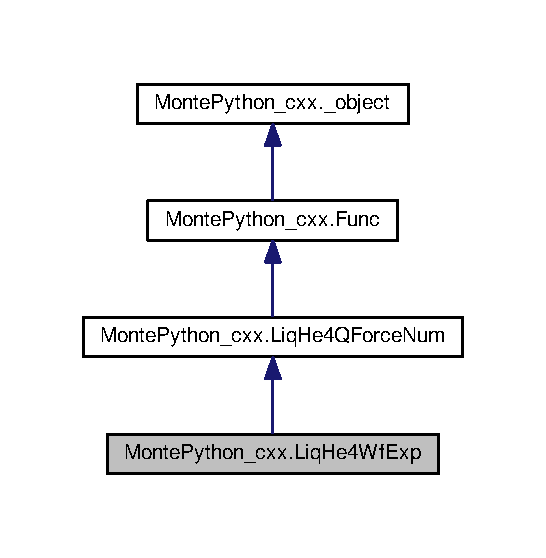
\includegraphics[width=262pt]{classMontePython__cxx_1_1LiqHe4WfExp__inherit__graph}
\end{center}
\end{figure}


Collaboration diagram for Monte\+Python\+\_\+cxx.\+Liq\+He4\+Wf\+Exp\+:
\nopagebreak
\begin{figure}[H]
\begin{center}
\leavevmode
\includegraphics[width=262pt]{classMontePython__cxx_1_1LiqHe4WfExp__coll__graph}
\end{center}
\end{figure}
\subsection*{Public Member Functions}
\begin{DoxyCompactItemize}
\item 
def \hyperlink{classMontePython__cxx_1_1LiqHe4WfExp_a19bd1b87c8225a8993198114d34e7ada}{set\+Params} (self, args)
\item 
def \hyperlink{classMontePython__cxx_1_1LiqHe4WfExp_a5fced62767bd46bf9399419eee79390f}{value\+Pt} (self, args)
\item 
def \hyperlink{classMontePython__cxx_1_1LiqHe4WfExp_a37f1b1995ce222cbde2336fd58b735bd}{\+\_\+\+\_\+call\+\_\+\+\_\+} (self, args)
\item 
def \hyperlink{classMontePython__cxx_1_1LiqHe4WfExp_ad6608765086bcae7a343f1dff4555180}{\+\_\+\+\_\+init\+\_\+\+\_\+} (self)
\end{DoxyCompactItemize}
\subsection*{Public Attributes}
\begin{DoxyCompactItemize}
\item 
\hypertarget{classMontePython__cxx_1_1LiqHe4WfExp_a28a3552f5da03de48636f5f1a9c05ecc}{}{\bfseries this}\label{classMontePython__cxx_1_1LiqHe4WfExp_a28a3552f5da03de48636f5f1a9c05ecc}

\end{DoxyCompactItemize}
\subsection*{Static Private Attributes}
\begin{DoxyCompactItemize}
\item 
\hypertarget{classMontePython__cxx_1_1LiqHe4WfExp_aa31f70202b64c481882ae5ac2cc349f7}{}dictionary {\bfseries \+\_\+\+\_\+swig\+\_\+setmethods\+\_\+\+\_\+} = \{\}\label{classMontePython__cxx_1_1LiqHe4WfExp_aa31f70202b64c481882ae5ac2cc349f7}

\item 
\hypertarget{classMontePython__cxx_1_1LiqHe4WfExp_aeac09c4cc7820215c0bed5cfd92277db}{}tuple {\bfseries \+\_\+\+\_\+setattr\+\_\+\+\_\+} = lambdaself,name,value\+:\+\_\+swig\+\_\+setattr(self, \hyperlink{classMontePython__cxx_1_1LiqHe4WfExp}{Liq\+He4\+Wf\+Exp}, name, value)\label{classMontePython__cxx_1_1LiqHe4WfExp_aeac09c4cc7820215c0bed5cfd92277db}

\item 
\hypertarget{classMontePython__cxx_1_1LiqHe4WfExp_a6d6517157ae1c561ae828f4834c235b8}{}dictionary {\bfseries \+\_\+\+\_\+swig\+\_\+getmethods\+\_\+\+\_\+} = \{\}\label{classMontePython__cxx_1_1LiqHe4WfExp_a6d6517157ae1c561ae828f4834c235b8}

\item 
\hypertarget{classMontePython__cxx_1_1LiqHe4WfExp_aca0f34fdb77c38e67fe37b274c144a5b}{}tuple {\bfseries \+\_\+\+\_\+getattr\+\_\+\+\_\+} = lambdaself,name\+:\+\_\+swig\+\_\+getattr(self, \hyperlink{classMontePython__cxx_1_1LiqHe4WfExp}{Liq\+He4\+Wf\+Exp}, name)\label{classMontePython__cxx_1_1LiqHe4WfExp_aca0f34fdb77c38e67fe37b274c144a5b}

\item 
\hypertarget{classMontePython__cxx_1_1LiqHe4WfExp_a0d14be73cca0a08bf1f30cfa787741af}{}{\bfseries \+\_\+\+\_\+repr\+\_\+\+\_\+} = \+\_\+swig\+\_\+repr\label{classMontePython__cxx_1_1LiqHe4WfExp_a0d14be73cca0a08bf1f30cfa787741af}

\item 
\hypertarget{classMontePython__cxx_1_1LiqHe4WfExp_acfe36ca0daa4ae086f1e06ea0fe66d3a}{}{\bfseries \+\_\+\+\_\+swig\+\_\+destroy\+\_\+\+\_\+} = \+\_\+\+Monte\+Python\+\_\+cxx.\+delete\+\_\+\+Liq\+He4\+Wf\+Exp\label{classMontePython__cxx_1_1LiqHe4WfExp_acfe36ca0daa4ae086f1e06ea0fe66d3a}

\end{DoxyCompactItemize}


\subsection{Detailed Description}
\begin{DoxyVerb}Proxy of C++ LiqHe4WfExp class\end{DoxyVerb}
 

\subsection{Constructor \& Destructor Documentation}
\hypertarget{classMontePython__cxx_1_1LiqHe4WfExp_ad6608765086bcae7a343f1dff4555180}{}\index{Monte\+Python\+\_\+cxx\+::\+Liq\+He4\+Wf\+Exp@{Monte\+Python\+\_\+cxx\+::\+Liq\+He4\+Wf\+Exp}!\+\_\+\+\_\+init\+\_\+\+\_\+@{\+\_\+\+\_\+init\+\_\+\+\_\+}}
\index{\+\_\+\+\_\+init\+\_\+\+\_\+@{\+\_\+\+\_\+init\+\_\+\+\_\+}!Monte\+Python\+\_\+cxx\+::\+Liq\+He4\+Wf\+Exp@{Monte\+Python\+\_\+cxx\+::\+Liq\+He4\+Wf\+Exp}}
\subsubsection[{\+\_\+\+\_\+init\+\_\+\+\_\+}]{\setlength{\rightskip}{0pt plus 5cm}def Monte\+Python\+\_\+cxx.\+Liq\+He4\+Wf\+Exp.\+\_\+\+\_\+init\+\_\+\+\_\+ (
\begin{DoxyParamCaption}
\item[{}]{self}
\end{DoxyParamCaption}
)}\label{classMontePython__cxx_1_1LiqHe4WfExp_ad6608765086bcae7a343f1dff4555180}
\begin{DoxyVerb}__init__(LiqHe4WfExp self) -> LiqHe4WfExp\end{DoxyVerb}
 

\subsection{Member Function Documentation}
\hypertarget{classMontePython__cxx_1_1LiqHe4WfExp_a37f1b1995ce222cbde2336fd58b735bd}{}\index{Monte\+Python\+\_\+cxx\+::\+Liq\+He4\+Wf\+Exp@{Monte\+Python\+\_\+cxx\+::\+Liq\+He4\+Wf\+Exp}!\+\_\+\+\_\+call\+\_\+\+\_\+@{\+\_\+\+\_\+call\+\_\+\+\_\+}}
\index{\+\_\+\+\_\+call\+\_\+\+\_\+@{\+\_\+\+\_\+call\+\_\+\+\_\+}!Monte\+Python\+\_\+cxx\+::\+Liq\+He4\+Wf\+Exp@{Monte\+Python\+\_\+cxx\+::\+Liq\+He4\+Wf\+Exp}}
\subsubsection[{\+\_\+\+\_\+call\+\_\+\+\_\+}]{\setlength{\rightskip}{0pt plus 5cm}def Monte\+Python\+\_\+cxx.\+Liq\+He4\+Wf\+Exp.\+\_\+\+\_\+call\+\_\+\+\_\+ (
\begin{DoxyParamCaption}
\item[{}]{self, }
\item[{}]{args}
\end{DoxyParamCaption}
)}\label{classMontePython__cxx_1_1LiqHe4WfExp_a37f1b1995ce222cbde2336fd58b735bd}
\begin{DoxyVerb}__call__(LiqHe4WfExp self, QickArray & pos) -> double\end{DoxyVerb}
 \hypertarget{classMontePython__cxx_1_1LiqHe4WfExp_a19bd1b87c8225a8993198114d34e7ada}{}\index{Monte\+Python\+\_\+cxx\+::\+Liq\+He4\+Wf\+Exp@{Monte\+Python\+\_\+cxx\+::\+Liq\+He4\+Wf\+Exp}!set\+Params@{set\+Params}}
\index{set\+Params@{set\+Params}!Monte\+Python\+\_\+cxx\+::\+Liq\+He4\+Wf\+Exp@{Monte\+Python\+\_\+cxx\+::\+Liq\+He4\+Wf\+Exp}}
\subsubsection[{set\+Params}]{\setlength{\rightskip}{0pt plus 5cm}def Monte\+Python\+\_\+cxx.\+Liq\+He4\+Wf\+Exp.\+set\+Params (
\begin{DoxyParamCaption}
\item[{}]{self, }
\item[{}]{args}
\end{DoxyParamCaption}
)}\label{classMontePython__cxx_1_1LiqHe4WfExp_a19bd1b87c8225a8993198114d34e7ada}
\begin{DoxyVerb}setParams(LiqHe4WfExp self, QickArray & params_)\end{DoxyVerb}
 \hypertarget{classMontePython__cxx_1_1LiqHe4WfExp_a5fced62767bd46bf9399419eee79390f}{}\index{Monte\+Python\+\_\+cxx\+::\+Liq\+He4\+Wf\+Exp@{Monte\+Python\+\_\+cxx\+::\+Liq\+He4\+Wf\+Exp}!value\+Pt@{value\+Pt}}
\index{value\+Pt@{value\+Pt}!Monte\+Python\+\_\+cxx\+::\+Liq\+He4\+Wf\+Exp@{Monte\+Python\+\_\+cxx\+::\+Liq\+He4\+Wf\+Exp}}
\subsubsection[{value\+Pt}]{\setlength{\rightskip}{0pt plus 5cm}def Monte\+Python\+\_\+cxx.\+Liq\+He4\+Wf\+Exp.\+value\+Pt (
\begin{DoxyParamCaption}
\item[{}]{self, }
\item[{}]{args}
\end{DoxyParamCaption}
)}\label{classMontePython__cxx_1_1LiqHe4WfExp_a5fced62767bd46bf9399419eee79390f}
\begin{DoxyVerb}valuePt(LiqHe4WfExp self, QickArray & pos) -> double\end{DoxyVerb}
 

The documentation for this class was generated from the following file\+:\begin{DoxyCompactItemize}
\item 
Monte\+Python\+\_\+cxx.\+py\end{DoxyCompactItemize}

\hypertarget{classMontePython__cxx_1_1MateuszLocalEnergy}{}\section{Monte\+Python\+\_\+cxx.\+Mateusz\+Local\+Energy Class Reference}
\label{classMontePython__cxx_1_1MateuszLocalEnergy}\index{Monte\+Python\+\_\+cxx.\+Mateusz\+Local\+Energy@{Monte\+Python\+\_\+cxx.\+Mateusz\+Local\+Energy}}


Inheritance diagram for Monte\+Python\+\_\+cxx.\+Mateusz\+Local\+Energy\+:
\nopagebreak
\begin{figure}[H]
\begin{center}
\leavevmode
\includegraphics[width=239pt]{classMontePython__cxx_1_1MateuszLocalEnergy__inherit__graph}
\end{center}
\end{figure}


Collaboration diagram for Monte\+Python\+\_\+cxx.\+Mateusz\+Local\+Energy\+:
\nopagebreak
\begin{figure}[H]
\begin{center}
\leavevmode
\includegraphics[width=239pt]{classMontePython__cxx_1_1MateuszLocalEnergy__coll__graph}
\end{center}
\end{figure}
\subsection*{Public Member Functions}
\begin{DoxyCompactItemize}
\item 
def \hyperlink{classMontePython__cxx_1_1MateuszLocalEnergy_a6630ef4e14d211b538d67cba1292331f}{set\+Params} (self, args)
\item 
def \hyperlink{classMontePython__cxx_1_1MateuszLocalEnergy_af7dce1501fd1f9b45ee1ec9cf504560d}{value\+Pt} (self, args)
\item 
def \hyperlink{classMontePython__cxx_1_1MateuszLocalEnergy_ad260692ecdec3770b2d92eec101e32ac}{\+\_\+\+\_\+call\+\_\+\+\_\+} (self, args)
\item 
def \hyperlink{classMontePython__cxx_1_1MateuszLocalEnergy_a170f9c04d3bebedddb1504e85b85ed68}{\+\_\+\+\_\+init\+\_\+\+\_\+} (self)
\end{DoxyCompactItemize}
\subsection*{Public Attributes}
\begin{DoxyCompactItemize}
\item 
\hypertarget{classMontePython__cxx_1_1MateuszLocalEnergy_a1f99f391d68ca0eb3e73c482ec178b45}{}{\bfseries this}\label{classMontePython__cxx_1_1MateuszLocalEnergy_a1f99f391d68ca0eb3e73c482ec178b45}

\end{DoxyCompactItemize}
\subsection*{Static Private Attributes}
\begin{DoxyCompactItemize}
\item 
\hypertarget{classMontePython__cxx_1_1MateuszLocalEnergy_a49a48dbcc19b52271babd78ad16de26c}{}dictionary {\bfseries \+\_\+\+\_\+swig\+\_\+setmethods\+\_\+\+\_\+} = \{\}\label{classMontePython__cxx_1_1MateuszLocalEnergy_a49a48dbcc19b52271babd78ad16de26c}

\item 
\hypertarget{classMontePython__cxx_1_1MateuszLocalEnergy_ad8c324d7e4e72e4fa33b3b7c1ec1ff99}{}tuple {\bfseries \+\_\+\+\_\+setattr\+\_\+\+\_\+} = lambdaself,name,value\+:\+\_\+swig\+\_\+setattr(self, \hyperlink{classMontePython__cxx_1_1MateuszLocalEnergy}{Mateusz\+Local\+Energy}, name, value)\label{classMontePython__cxx_1_1MateuszLocalEnergy_ad8c324d7e4e72e4fa33b3b7c1ec1ff99}

\item 
\hypertarget{classMontePython__cxx_1_1MateuszLocalEnergy_ac0189d8c162305bf0fb6568b19eebdf5}{}dictionary {\bfseries \+\_\+\+\_\+swig\+\_\+getmethods\+\_\+\+\_\+} = \{\}\label{classMontePython__cxx_1_1MateuszLocalEnergy_ac0189d8c162305bf0fb6568b19eebdf5}

\item 
\hypertarget{classMontePython__cxx_1_1MateuszLocalEnergy_aa9fac2867a0f407a89002a1641f158e5}{}tuple {\bfseries \+\_\+\+\_\+getattr\+\_\+\+\_\+} = lambdaself,name\+:\+\_\+swig\+\_\+getattr(self, \hyperlink{classMontePython__cxx_1_1MateuszLocalEnergy}{Mateusz\+Local\+Energy}, name)\label{classMontePython__cxx_1_1MateuszLocalEnergy_aa9fac2867a0f407a89002a1641f158e5}

\item 
\hypertarget{classMontePython__cxx_1_1MateuszLocalEnergy_afcfac0f89b9f8a59f88a76b2933eb6ca}{}{\bfseries \+\_\+\+\_\+repr\+\_\+\+\_\+} = \+\_\+swig\+\_\+repr\label{classMontePython__cxx_1_1MateuszLocalEnergy_afcfac0f89b9f8a59f88a76b2933eb6ca}

\item 
\hypertarget{classMontePython__cxx_1_1MateuszLocalEnergy_a88b3341c43ab2bd32ecb447e7e82e9de}{}{\bfseries \+\_\+\+\_\+swig\+\_\+destroy\+\_\+\+\_\+} = \+\_\+\+Monte\+Python\+\_\+cxx.\+delete\+\_\+\+Mateusz\+Local\+Energy\label{classMontePython__cxx_1_1MateuszLocalEnergy_a88b3341c43ab2bd32ecb447e7e82e9de}

\end{DoxyCompactItemize}


\subsection{Detailed Description}
\begin{DoxyVerb}Proxy of C++ MateuszLocalEnergy class\end{DoxyVerb}
 

\subsection{Constructor \& Destructor Documentation}
\hypertarget{classMontePython__cxx_1_1MateuszLocalEnergy_a170f9c04d3bebedddb1504e85b85ed68}{}\index{Monte\+Python\+\_\+cxx\+::\+Mateusz\+Local\+Energy@{Monte\+Python\+\_\+cxx\+::\+Mateusz\+Local\+Energy}!\+\_\+\+\_\+init\+\_\+\+\_\+@{\+\_\+\+\_\+init\+\_\+\+\_\+}}
\index{\+\_\+\+\_\+init\+\_\+\+\_\+@{\+\_\+\+\_\+init\+\_\+\+\_\+}!Monte\+Python\+\_\+cxx\+::\+Mateusz\+Local\+Energy@{Monte\+Python\+\_\+cxx\+::\+Mateusz\+Local\+Energy}}
\subsubsection[{\+\_\+\+\_\+init\+\_\+\+\_\+}]{\setlength{\rightskip}{0pt plus 5cm}def Monte\+Python\+\_\+cxx.\+Mateusz\+Local\+Energy.\+\_\+\+\_\+init\+\_\+\+\_\+ (
\begin{DoxyParamCaption}
\item[{}]{self}
\end{DoxyParamCaption}
)}\label{classMontePython__cxx_1_1MateuszLocalEnergy_a170f9c04d3bebedddb1504e85b85ed68}
\begin{DoxyVerb}__init__(MateuszLocalEnergy self) -> MateuszLocalEnergy\end{DoxyVerb}
 

\subsection{Member Function Documentation}
\hypertarget{classMontePython__cxx_1_1MateuszLocalEnergy_ad260692ecdec3770b2d92eec101e32ac}{}\index{Monte\+Python\+\_\+cxx\+::\+Mateusz\+Local\+Energy@{Monte\+Python\+\_\+cxx\+::\+Mateusz\+Local\+Energy}!\+\_\+\+\_\+call\+\_\+\+\_\+@{\+\_\+\+\_\+call\+\_\+\+\_\+}}
\index{\+\_\+\+\_\+call\+\_\+\+\_\+@{\+\_\+\+\_\+call\+\_\+\+\_\+}!Monte\+Python\+\_\+cxx\+::\+Mateusz\+Local\+Energy@{Monte\+Python\+\_\+cxx\+::\+Mateusz\+Local\+Energy}}
\subsubsection[{\+\_\+\+\_\+call\+\_\+\+\_\+}]{\setlength{\rightskip}{0pt plus 5cm}def Monte\+Python\+\_\+cxx.\+Mateusz\+Local\+Energy.\+\_\+\+\_\+call\+\_\+\+\_\+ (
\begin{DoxyParamCaption}
\item[{}]{self, }
\item[{}]{args}
\end{DoxyParamCaption}
)}\label{classMontePython__cxx_1_1MateuszLocalEnergy_ad260692ecdec3770b2d92eec101e32ac}
\begin{DoxyVerb}__call__(MateuszLocalEnergy self, QickArray & pos) -> double\end{DoxyVerb}
 \hypertarget{classMontePython__cxx_1_1MateuszLocalEnergy_a6630ef4e14d211b538d67cba1292331f}{}\index{Monte\+Python\+\_\+cxx\+::\+Mateusz\+Local\+Energy@{Monte\+Python\+\_\+cxx\+::\+Mateusz\+Local\+Energy}!set\+Params@{set\+Params}}
\index{set\+Params@{set\+Params}!Monte\+Python\+\_\+cxx\+::\+Mateusz\+Local\+Energy@{Monte\+Python\+\_\+cxx\+::\+Mateusz\+Local\+Energy}}
\subsubsection[{set\+Params}]{\setlength{\rightskip}{0pt plus 5cm}def Monte\+Python\+\_\+cxx.\+Mateusz\+Local\+Energy.\+set\+Params (
\begin{DoxyParamCaption}
\item[{}]{self, }
\item[{}]{args}
\end{DoxyParamCaption}
)}\label{classMontePython__cxx_1_1MateuszLocalEnergy_a6630ef4e14d211b538d67cba1292331f}
\begin{DoxyVerb}setParams(MateuszLocalEnergy self, QickArray & params_)\end{DoxyVerb}
 \hypertarget{classMontePython__cxx_1_1MateuszLocalEnergy_af7dce1501fd1f9b45ee1ec9cf504560d}{}\index{Monte\+Python\+\_\+cxx\+::\+Mateusz\+Local\+Energy@{Monte\+Python\+\_\+cxx\+::\+Mateusz\+Local\+Energy}!value\+Pt@{value\+Pt}}
\index{value\+Pt@{value\+Pt}!Monte\+Python\+\_\+cxx\+::\+Mateusz\+Local\+Energy@{Monte\+Python\+\_\+cxx\+::\+Mateusz\+Local\+Energy}}
\subsubsection[{value\+Pt}]{\setlength{\rightskip}{0pt plus 5cm}def Monte\+Python\+\_\+cxx.\+Mateusz\+Local\+Energy.\+value\+Pt (
\begin{DoxyParamCaption}
\item[{}]{self, }
\item[{}]{args}
\end{DoxyParamCaption}
)}\label{classMontePython__cxx_1_1MateuszLocalEnergy_af7dce1501fd1f9b45ee1ec9cf504560d}
\begin{DoxyVerb}valuePt(MateuszLocalEnergy self, QickArray & pos) -> double\end{DoxyVerb}
 

The documentation for this class was generated from the following file\+:\begin{DoxyCompactItemize}
\item 
Monte\+Python\+\_\+cxx.\+py\end{DoxyCompactItemize}

\hypertarget{classMontePython__cxx_1_1MateuszPotentialEnergy}{}\section{Monte\+Python\+\_\+cxx.\+Mateusz\+Potential\+Energy Class Reference}
\label{classMontePython__cxx_1_1MateuszPotentialEnergy}\index{Monte\+Python\+\_\+cxx.\+Mateusz\+Potential\+Energy@{Monte\+Python\+\_\+cxx.\+Mateusz\+Potential\+Energy}}


Inheritance diagram for Monte\+Python\+\_\+cxx.\+Mateusz\+Potential\+Energy\+:
\nopagebreak
\begin{figure}[H]
\begin{center}
\leavevmode
\includegraphics[width=254pt]{classMontePython__cxx_1_1MateuszPotentialEnergy__inherit__graph}
\end{center}
\end{figure}


Collaboration diagram for Monte\+Python\+\_\+cxx.\+Mateusz\+Potential\+Energy\+:
\nopagebreak
\begin{figure}[H]
\begin{center}
\leavevmode
\includegraphics[width=254pt]{classMontePython__cxx_1_1MateuszPotentialEnergy__coll__graph}
\end{center}
\end{figure}
\subsection*{Public Member Functions}
\begin{DoxyCompactItemize}
\item 
def \hyperlink{classMontePython__cxx_1_1MateuszPotentialEnergy_a2484565397734518405b714db0d04a42}{set\+Params} (self, args)
\item 
def \hyperlink{classMontePython__cxx_1_1MateuszPotentialEnergy_a0fd1acc82f2f2fb35d9576722a9b50ae}{value\+Pt} (self, args)
\item 
def \hyperlink{classMontePython__cxx_1_1MateuszPotentialEnergy_ad516dad153c4454a9fc2ab0d5a5a9e3a}{\+\_\+\+\_\+call\+\_\+\+\_\+} (self, args)
\item 
def \hyperlink{classMontePython__cxx_1_1MateuszPotentialEnergy_a492dbf538581f57d97b2b89dae68ed22}{\+\_\+\+\_\+init\+\_\+\+\_\+} (self)
\end{DoxyCompactItemize}
\subsection*{Public Attributes}
\begin{DoxyCompactItemize}
\item 
\hypertarget{classMontePython__cxx_1_1MateuszPotentialEnergy_afa39371918d5c244c93fd23d02a59fd1}{}{\bfseries this}\label{classMontePython__cxx_1_1MateuszPotentialEnergy_afa39371918d5c244c93fd23d02a59fd1}

\end{DoxyCompactItemize}
\subsection*{Static Private Attributes}
\begin{DoxyCompactItemize}
\item 
\hypertarget{classMontePython__cxx_1_1MateuszPotentialEnergy_a4602d1eb20498bb085a4fcece953b842}{}dictionary {\bfseries \+\_\+\+\_\+swig\+\_\+setmethods\+\_\+\+\_\+} = \{\}\label{classMontePython__cxx_1_1MateuszPotentialEnergy_a4602d1eb20498bb085a4fcece953b842}

\item 
\hypertarget{classMontePython__cxx_1_1MateuszPotentialEnergy_ae58cbfd02c7150eacd37fc96b03b5389}{}tuple {\bfseries \+\_\+\+\_\+setattr\+\_\+\+\_\+} = lambdaself,name,value\+:\+\_\+swig\+\_\+setattr(self, \hyperlink{classMontePython__cxx_1_1MateuszPotentialEnergy}{Mateusz\+Potential\+Energy}, name, value)\label{classMontePython__cxx_1_1MateuszPotentialEnergy_ae58cbfd02c7150eacd37fc96b03b5389}

\item 
\hypertarget{classMontePython__cxx_1_1MateuszPotentialEnergy_a288108983c3a137de3e1bf47b3b2bd0b}{}dictionary {\bfseries \+\_\+\+\_\+swig\+\_\+getmethods\+\_\+\+\_\+} = \{\}\label{classMontePython__cxx_1_1MateuszPotentialEnergy_a288108983c3a137de3e1bf47b3b2bd0b}

\item 
\hypertarget{classMontePython__cxx_1_1MateuszPotentialEnergy_a7225991c5ed16702697aa26c59875bf8}{}tuple {\bfseries \+\_\+\+\_\+getattr\+\_\+\+\_\+} = lambdaself,name\+:\+\_\+swig\+\_\+getattr(self, \hyperlink{classMontePython__cxx_1_1MateuszPotentialEnergy}{Mateusz\+Potential\+Energy}, name)\label{classMontePython__cxx_1_1MateuszPotentialEnergy_a7225991c5ed16702697aa26c59875bf8}

\item 
\hypertarget{classMontePython__cxx_1_1MateuszPotentialEnergy_a9b1d5e0cf78196e10c4f774e3c1de679}{}{\bfseries \+\_\+\+\_\+repr\+\_\+\+\_\+} = \+\_\+swig\+\_\+repr\label{classMontePython__cxx_1_1MateuszPotentialEnergy_a9b1d5e0cf78196e10c4f774e3c1de679}

\item 
\hypertarget{classMontePython__cxx_1_1MateuszPotentialEnergy_a6df330cd9ea8624dd38aa103bed30654}{}{\bfseries \+\_\+\+\_\+swig\+\_\+destroy\+\_\+\+\_\+} = \+\_\+\+Monte\+Python\+\_\+cxx.\+delete\+\_\+\+Mateusz\+Potential\+Energy\label{classMontePython__cxx_1_1MateuszPotentialEnergy_a6df330cd9ea8624dd38aa103bed30654}

\end{DoxyCompactItemize}


\subsection{Detailed Description}
\begin{DoxyVerb}Proxy of C++ MateuszPotentialEnergy class\end{DoxyVerb}
 

\subsection{Constructor \& Destructor Documentation}
\hypertarget{classMontePython__cxx_1_1MateuszPotentialEnergy_a492dbf538581f57d97b2b89dae68ed22}{}\index{Monte\+Python\+\_\+cxx\+::\+Mateusz\+Potential\+Energy@{Monte\+Python\+\_\+cxx\+::\+Mateusz\+Potential\+Energy}!\+\_\+\+\_\+init\+\_\+\+\_\+@{\+\_\+\+\_\+init\+\_\+\+\_\+}}
\index{\+\_\+\+\_\+init\+\_\+\+\_\+@{\+\_\+\+\_\+init\+\_\+\+\_\+}!Monte\+Python\+\_\+cxx\+::\+Mateusz\+Potential\+Energy@{Monte\+Python\+\_\+cxx\+::\+Mateusz\+Potential\+Energy}}
\subsubsection[{\+\_\+\+\_\+init\+\_\+\+\_\+}]{\setlength{\rightskip}{0pt plus 5cm}def Monte\+Python\+\_\+cxx.\+Mateusz\+Potential\+Energy.\+\_\+\+\_\+init\+\_\+\+\_\+ (
\begin{DoxyParamCaption}
\item[{}]{self}
\end{DoxyParamCaption}
)}\label{classMontePython__cxx_1_1MateuszPotentialEnergy_a492dbf538581f57d97b2b89dae68ed22}
\begin{DoxyVerb}__init__(MateuszPotentialEnergy self) -> MateuszPotentialEnergy\end{DoxyVerb}
 

\subsection{Member Function Documentation}
\hypertarget{classMontePython__cxx_1_1MateuszPotentialEnergy_ad516dad153c4454a9fc2ab0d5a5a9e3a}{}\index{Monte\+Python\+\_\+cxx\+::\+Mateusz\+Potential\+Energy@{Monte\+Python\+\_\+cxx\+::\+Mateusz\+Potential\+Energy}!\+\_\+\+\_\+call\+\_\+\+\_\+@{\+\_\+\+\_\+call\+\_\+\+\_\+}}
\index{\+\_\+\+\_\+call\+\_\+\+\_\+@{\+\_\+\+\_\+call\+\_\+\+\_\+}!Monte\+Python\+\_\+cxx\+::\+Mateusz\+Potential\+Energy@{Monte\+Python\+\_\+cxx\+::\+Mateusz\+Potential\+Energy}}
\subsubsection[{\+\_\+\+\_\+call\+\_\+\+\_\+}]{\setlength{\rightskip}{0pt plus 5cm}def Monte\+Python\+\_\+cxx.\+Mateusz\+Potential\+Energy.\+\_\+\+\_\+call\+\_\+\+\_\+ (
\begin{DoxyParamCaption}
\item[{}]{self, }
\item[{}]{args}
\end{DoxyParamCaption}
)}\label{classMontePython__cxx_1_1MateuszPotentialEnergy_ad516dad153c4454a9fc2ab0d5a5a9e3a}
\begin{DoxyVerb}__call__(MateuszPotentialEnergy self, QickArray & pos) -> double\end{DoxyVerb}
 \hypertarget{classMontePython__cxx_1_1MateuszPotentialEnergy_a2484565397734518405b714db0d04a42}{}\index{Monte\+Python\+\_\+cxx\+::\+Mateusz\+Potential\+Energy@{Monte\+Python\+\_\+cxx\+::\+Mateusz\+Potential\+Energy}!set\+Params@{set\+Params}}
\index{set\+Params@{set\+Params}!Monte\+Python\+\_\+cxx\+::\+Mateusz\+Potential\+Energy@{Monte\+Python\+\_\+cxx\+::\+Mateusz\+Potential\+Energy}}
\subsubsection[{set\+Params}]{\setlength{\rightskip}{0pt plus 5cm}def Monte\+Python\+\_\+cxx.\+Mateusz\+Potential\+Energy.\+set\+Params (
\begin{DoxyParamCaption}
\item[{}]{self, }
\item[{}]{args}
\end{DoxyParamCaption}
)}\label{classMontePython__cxx_1_1MateuszPotentialEnergy_a2484565397734518405b714db0d04a42}
\begin{DoxyVerb}setParams(MateuszPotentialEnergy self, QickArray & params_)\end{DoxyVerb}
 \hypertarget{classMontePython__cxx_1_1MateuszPotentialEnergy_a0fd1acc82f2f2fb35d9576722a9b50ae}{}\index{Monte\+Python\+\_\+cxx\+::\+Mateusz\+Potential\+Energy@{Monte\+Python\+\_\+cxx\+::\+Mateusz\+Potential\+Energy}!value\+Pt@{value\+Pt}}
\index{value\+Pt@{value\+Pt}!Monte\+Python\+\_\+cxx\+::\+Mateusz\+Potential\+Energy@{Monte\+Python\+\_\+cxx\+::\+Mateusz\+Potential\+Energy}}
\subsubsection[{value\+Pt}]{\setlength{\rightskip}{0pt plus 5cm}def Monte\+Python\+\_\+cxx.\+Mateusz\+Potential\+Energy.\+value\+Pt (
\begin{DoxyParamCaption}
\item[{}]{self, }
\item[{}]{args}
\end{DoxyParamCaption}
)}\label{classMontePython__cxx_1_1MateuszPotentialEnergy_a0fd1acc82f2f2fb35d9576722a9b50ae}
\begin{DoxyVerb}valuePt(MateuszPotentialEnergy self, QickArray & pos) -> double\end{DoxyVerb}
 

The documentation for this class was generated from the following file\+:\begin{DoxyCompactItemize}
\item 
Monte\+Python\+\_\+cxx.\+py\end{DoxyCompactItemize}

\hypertarget{classMontePython__cxx_1_1MateuszQForce}{}\section{Monte\+Python\+\_\+cxx.\+Mateusz\+Q\+Force Class Reference}
\label{classMontePython__cxx_1_1MateuszQForce}\index{Monte\+Python\+\_\+cxx.\+Mateusz\+Q\+Force@{Monte\+Python\+\_\+cxx.\+Mateusz\+Q\+Force}}


Inheritance diagram for Monte\+Python\+\_\+cxx.\+Mateusz\+Q\+Force\+:
\nopagebreak
\begin{figure}[H]
\begin{center}
\leavevmode
\includegraphics[width=248pt]{classMontePython__cxx_1_1MateuszQForce__inherit__graph}
\end{center}
\end{figure}


Collaboration diagram for Monte\+Python\+\_\+cxx.\+Mateusz\+Q\+Force\+:
\nopagebreak
\begin{figure}[H]
\begin{center}
\leavevmode
\includegraphics[width=248pt]{classMontePython__cxx_1_1MateuszQForce__coll__graph}
\end{center}
\end{figure}
\subsection*{Public Member Functions}
\begin{DoxyCompactItemize}
\item 
def \hyperlink{classMontePython__cxx_1_1MateuszQForce_ae83e49e08e124f5bfebeda4b90216d2f}{set\+Params} (self, args)
\item 
def \hyperlink{classMontePython__cxx_1_1MateuszQForce_a81cceed0d27f93b55b5dc20ff270bdc0}{value\+Pt} (self, args)
\item 
def \hyperlink{classMontePython__cxx_1_1MateuszQForce_ab2f6ab527b2898fe7ed8421bb2e94218}{\+\_\+\+\_\+call\+\_\+\+\_\+} (self, args)
\item 
def \hyperlink{classMontePython__cxx_1_1MateuszQForce_a6eb02942deedc143d1e175108ae161bd}{\+\_\+\+\_\+init\+\_\+\+\_\+} (self)
\end{DoxyCompactItemize}
\subsection*{Public Attributes}
\begin{DoxyCompactItemize}
\item 
\hypertarget{classMontePython__cxx_1_1MateuszQForce_a4cb171bb31ae6f6721fa508e8cd92bd6}{}{\bfseries this}\label{classMontePython__cxx_1_1MateuszQForce_a4cb171bb31ae6f6721fa508e8cd92bd6}

\end{DoxyCompactItemize}
\subsection*{Static Private Attributes}
\begin{DoxyCompactItemize}
\item 
\hypertarget{classMontePython__cxx_1_1MateuszQForce_a7e52680e3c2849bf6b4c898a88d0d67c}{}dictionary {\bfseries \+\_\+\+\_\+swig\+\_\+setmethods\+\_\+\+\_\+} = \{\}\label{classMontePython__cxx_1_1MateuszQForce_a7e52680e3c2849bf6b4c898a88d0d67c}

\item 
\hypertarget{classMontePython__cxx_1_1MateuszQForce_a5a91ac21598979d78de32ea076434397}{}tuple {\bfseries \+\_\+\+\_\+setattr\+\_\+\+\_\+} = lambdaself,name,value\+:\+\_\+swig\+\_\+setattr(self, \hyperlink{classMontePython__cxx_1_1MateuszQForce}{Mateusz\+Q\+Force}, name, value)\label{classMontePython__cxx_1_1MateuszQForce_a5a91ac21598979d78de32ea076434397}

\item 
\hypertarget{classMontePython__cxx_1_1MateuszQForce_a8ec498fb626a4869b5a60b6a3f8d6682}{}dictionary {\bfseries \+\_\+\+\_\+swig\+\_\+getmethods\+\_\+\+\_\+} = \{\}\label{classMontePython__cxx_1_1MateuszQForce_a8ec498fb626a4869b5a60b6a3f8d6682}

\item 
\hypertarget{classMontePython__cxx_1_1MateuszQForce_a02cf593107bca06d77303ef2960764a4}{}tuple {\bfseries \+\_\+\+\_\+getattr\+\_\+\+\_\+} = lambdaself,name\+:\+\_\+swig\+\_\+getattr(self, \hyperlink{classMontePython__cxx_1_1MateuszQForce}{Mateusz\+Q\+Force}, name)\label{classMontePython__cxx_1_1MateuszQForce_a02cf593107bca06d77303ef2960764a4}

\item 
\hypertarget{classMontePython__cxx_1_1MateuszQForce_a58045981c0021be49b8b837e6b504ddb}{}{\bfseries \+\_\+\+\_\+repr\+\_\+\+\_\+} = \+\_\+swig\+\_\+repr\label{classMontePython__cxx_1_1MateuszQForce_a58045981c0021be49b8b837e6b504ddb}

\item 
\hypertarget{classMontePython__cxx_1_1MateuszQForce_a12619f34d5b9853c6c9088f5dea81ea5}{}{\bfseries \+\_\+\+\_\+swig\+\_\+destroy\+\_\+\+\_\+} = \+\_\+\+Monte\+Python\+\_\+cxx.\+delete\+\_\+\+Mateusz\+Q\+Force\label{classMontePython__cxx_1_1MateuszQForce_a12619f34d5b9853c6c9088f5dea81ea5}

\end{DoxyCompactItemize}


\subsection{Detailed Description}
\begin{DoxyVerb}Proxy of C++ MateuszQForce class\end{DoxyVerb}
 

\subsection{Constructor \& Destructor Documentation}
\hypertarget{classMontePython__cxx_1_1MateuszQForce_a6eb02942deedc143d1e175108ae161bd}{}\index{Monte\+Python\+\_\+cxx\+::\+Mateusz\+Q\+Force@{Monte\+Python\+\_\+cxx\+::\+Mateusz\+Q\+Force}!\+\_\+\+\_\+init\+\_\+\+\_\+@{\+\_\+\+\_\+init\+\_\+\+\_\+}}
\index{\+\_\+\+\_\+init\+\_\+\+\_\+@{\+\_\+\+\_\+init\+\_\+\+\_\+}!Monte\+Python\+\_\+cxx\+::\+Mateusz\+Q\+Force@{Monte\+Python\+\_\+cxx\+::\+Mateusz\+Q\+Force}}
\subsubsection[{\+\_\+\+\_\+init\+\_\+\+\_\+}]{\setlength{\rightskip}{0pt plus 5cm}def Monte\+Python\+\_\+cxx.\+Mateusz\+Q\+Force.\+\_\+\+\_\+init\+\_\+\+\_\+ (
\begin{DoxyParamCaption}
\item[{}]{self}
\end{DoxyParamCaption}
)}\label{classMontePython__cxx_1_1MateuszQForce_a6eb02942deedc143d1e175108ae161bd}
\begin{DoxyVerb}__init__(MateuszQForce self) -> MateuszQForce\end{DoxyVerb}
 

\subsection{Member Function Documentation}
\hypertarget{classMontePython__cxx_1_1MateuszQForce_ab2f6ab527b2898fe7ed8421bb2e94218}{}\index{Monte\+Python\+\_\+cxx\+::\+Mateusz\+Q\+Force@{Monte\+Python\+\_\+cxx\+::\+Mateusz\+Q\+Force}!\+\_\+\+\_\+call\+\_\+\+\_\+@{\+\_\+\+\_\+call\+\_\+\+\_\+}}
\index{\+\_\+\+\_\+call\+\_\+\+\_\+@{\+\_\+\+\_\+call\+\_\+\+\_\+}!Monte\+Python\+\_\+cxx\+::\+Mateusz\+Q\+Force@{Monte\+Python\+\_\+cxx\+::\+Mateusz\+Q\+Force}}
\subsubsection[{\+\_\+\+\_\+call\+\_\+\+\_\+}]{\setlength{\rightskip}{0pt plus 5cm}def Monte\+Python\+\_\+cxx.\+Mateusz\+Q\+Force.\+\_\+\+\_\+call\+\_\+\+\_\+ (
\begin{DoxyParamCaption}
\item[{}]{self, }
\item[{}]{args}
\end{DoxyParamCaption}
)}\label{classMontePython__cxx_1_1MateuszQForce_ab2f6ab527b2898fe7ed8421bb2e94218}
\begin{DoxyVerb}__call__(MateuszQForce self, QickArray & pos, bool dummy) -> QickArray &\end{DoxyVerb}
 \hypertarget{classMontePython__cxx_1_1MateuszQForce_ae83e49e08e124f5bfebeda4b90216d2f}{}\index{Monte\+Python\+\_\+cxx\+::\+Mateusz\+Q\+Force@{Monte\+Python\+\_\+cxx\+::\+Mateusz\+Q\+Force}!set\+Params@{set\+Params}}
\index{set\+Params@{set\+Params}!Monte\+Python\+\_\+cxx\+::\+Mateusz\+Q\+Force@{Monte\+Python\+\_\+cxx\+::\+Mateusz\+Q\+Force}}
\subsubsection[{set\+Params}]{\setlength{\rightskip}{0pt plus 5cm}def Monte\+Python\+\_\+cxx.\+Mateusz\+Q\+Force.\+set\+Params (
\begin{DoxyParamCaption}
\item[{}]{self, }
\item[{}]{args}
\end{DoxyParamCaption}
)}\label{classMontePython__cxx_1_1MateuszQForce_ae83e49e08e124f5bfebeda4b90216d2f}
\begin{DoxyVerb}setParams(MateuszQForce self, QickArray & params_)\end{DoxyVerb}
 \hypertarget{classMontePython__cxx_1_1MateuszQForce_a81cceed0d27f93b55b5dc20ff270bdc0}{}\index{Monte\+Python\+\_\+cxx\+::\+Mateusz\+Q\+Force@{Monte\+Python\+\_\+cxx\+::\+Mateusz\+Q\+Force}!value\+Pt@{value\+Pt}}
\index{value\+Pt@{value\+Pt}!Monte\+Python\+\_\+cxx\+::\+Mateusz\+Q\+Force@{Monte\+Python\+\_\+cxx\+::\+Mateusz\+Q\+Force}}
\subsubsection[{value\+Pt}]{\setlength{\rightskip}{0pt plus 5cm}def Monte\+Python\+\_\+cxx.\+Mateusz\+Q\+Force.\+value\+Pt (
\begin{DoxyParamCaption}
\item[{}]{self, }
\item[{}]{args}
\end{DoxyParamCaption}
)}\label{classMontePython__cxx_1_1MateuszQForce_a81cceed0d27f93b55b5dc20ff270bdc0}
\begin{DoxyVerb}valuePt(MateuszQForce self, QickArray & pos, bool dummy) -> QickArray &\end{DoxyVerb}
 

The documentation for this class was generated from the following file\+:\begin{DoxyCompactItemize}
\item 
Monte\+Python\+\_\+cxx.\+py\end{DoxyCompactItemize}

\hypertarget{classMontePython__cxx_1_1MateuszWave}{}\section{Monte\+Python\+\_\+cxx.\+Mateusz\+Wave Class Reference}
\label{classMontePython__cxx_1_1MateuszWave}\index{Monte\+Python\+\_\+cxx.\+Mateusz\+Wave@{Monte\+Python\+\_\+cxx.\+Mateusz\+Wave}}


Inheritance diagram for Monte\+Python\+\_\+cxx.\+Mateusz\+Wave\+:
\nopagebreak
\begin{figure}[H]
\begin{center}
\leavevmode
\includegraphics[width=241pt]{classMontePython__cxx_1_1MateuszWave__inherit__graph}
\end{center}
\end{figure}


Collaboration diagram for Monte\+Python\+\_\+cxx.\+Mateusz\+Wave\+:
\nopagebreak
\begin{figure}[H]
\begin{center}
\leavevmode
\includegraphics[width=241pt]{classMontePython__cxx_1_1MateuszWave__coll__graph}
\end{center}
\end{figure}
\subsection*{Public Member Functions}
\begin{DoxyCompactItemize}
\item 
def \hyperlink{classMontePython__cxx_1_1MateuszWave_af442152e4bf32618aa23f5389141ce83}{set\+Params} (self, args)
\item 
def \hyperlink{classMontePython__cxx_1_1MateuszWave_ab0f075c0eee21f7eb1e4ec2dfdd98d74}{value\+Pt} (self, args)
\item 
def \hyperlink{classMontePython__cxx_1_1MateuszWave_af05950ecb1b16571f7da05230f318fa2}{\+\_\+\+\_\+call\+\_\+\+\_\+} (self, args)
\item 
def \hyperlink{classMontePython__cxx_1_1MateuszWave_a956b0919640617a3b036d6c120e31ced}{\+\_\+\+\_\+init\+\_\+\+\_\+} (self)
\end{DoxyCompactItemize}
\subsection*{Public Attributes}
\begin{DoxyCompactItemize}
\item 
\hypertarget{classMontePython__cxx_1_1MateuszWave_a6b1a7f41d2fc9c4a3c50de14e052970d}{}{\bfseries this}\label{classMontePython__cxx_1_1MateuszWave_a6b1a7f41d2fc9c4a3c50de14e052970d}

\end{DoxyCompactItemize}
\subsection*{Static Private Attributes}
\begin{DoxyCompactItemize}
\item 
\hypertarget{classMontePython__cxx_1_1MateuszWave_ab2e52f9c7aa5df9b76c17da7b2930a51}{}dictionary {\bfseries \+\_\+\+\_\+swig\+\_\+setmethods\+\_\+\+\_\+} = \{\}\label{classMontePython__cxx_1_1MateuszWave_ab2e52f9c7aa5df9b76c17da7b2930a51}

\item 
\hypertarget{classMontePython__cxx_1_1MateuszWave_ad8f57e18e6b4b55449828e59b29d5f69}{}tuple {\bfseries \+\_\+\+\_\+setattr\+\_\+\+\_\+} = lambdaself,name,value\+:\+\_\+swig\+\_\+setattr(self, \hyperlink{classMontePython__cxx_1_1MateuszWave}{Mateusz\+Wave}, name, value)\label{classMontePython__cxx_1_1MateuszWave_ad8f57e18e6b4b55449828e59b29d5f69}

\item 
\hypertarget{classMontePython__cxx_1_1MateuszWave_a68533aa6fa641a758e83be51b5332505}{}dictionary {\bfseries \+\_\+\+\_\+swig\+\_\+getmethods\+\_\+\+\_\+} = \{\}\label{classMontePython__cxx_1_1MateuszWave_a68533aa6fa641a758e83be51b5332505}

\item 
\hypertarget{classMontePython__cxx_1_1MateuszWave_a41b61616903308c373a461e8c0954614}{}tuple {\bfseries \+\_\+\+\_\+getattr\+\_\+\+\_\+} = lambdaself,name\+:\+\_\+swig\+\_\+getattr(self, \hyperlink{classMontePython__cxx_1_1MateuszWave}{Mateusz\+Wave}, name)\label{classMontePython__cxx_1_1MateuszWave_a41b61616903308c373a461e8c0954614}

\item 
\hypertarget{classMontePython__cxx_1_1MateuszWave_aba9cf9af146411882ef68951645b8017}{}{\bfseries \+\_\+\+\_\+repr\+\_\+\+\_\+} = \+\_\+swig\+\_\+repr\label{classMontePython__cxx_1_1MateuszWave_aba9cf9af146411882ef68951645b8017}

\item 
\hypertarget{classMontePython__cxx_1_1MateuszWave_a5f01de4a6d7564a736156d89a835b54c}{}{\bfseries \+\_\+\+\_\+swig\+\_\+destroy\+\_\+\+\_\+} = \+\_\+\+Monte\+Python\+\_\+cxx.\+delete\+\_\+\+Mateusz\+Wave\label{classMontePython__cxx_1_1MateuszWave_a5f01de4a6d7564a736156d89a835b54c}

\end{DoxyCompactItemize}


\subsection{Detailed Description}
\begin{DoxyVerb}Proxy of C++ MateuszWave class\end{DoxyVerb}
 

\subsection{Constructor \& Destructor Documentation}
\hypertarget{classMontePython__cxx_1_1MateuszWave_a956b0919640617a3b036d6c120e31ced}{}\index{Monte\+Python\+\_\+cxx\+::\+Mateusz\+Wave@{Monte\+Python\+\_\+cxx\+::\+Mateusz\+Wave}!\+\_\+\+\_\+init\+\_\+\+\_\+@{\+\_\+\+\_\+init\+\_\+\+\_\+}}
\index{\+\_\+\+\_\+init\+\_\+\+\_\+@{\+\_\+\+\_\+init\+\_\+\+\_\+}!Monte\+Python\+\_\+cxx\+::\+Mateusz\+Wave@{Monte\+Python\+\_\+cxx\+::\+Mateusz\+Wave}}
\subsubsection[{\+\_\+\+\_\+init\+\_\+\+\_\+}]{\setlength{\rightskip}{0pt plus 5cm}def Monte\+Python\+\_\+cxx.\+Mateusz\+Wave.\+\_\+\+\_\+init\+\_\+\+\_\+ (
\begin{DoxyParamCaption}
\item[{}]{self}
\end{DoxyParamCaption}
)}\label{classMontePython__cxx_1_1MateuszWave_a956b0919640617a3b036d6c120e31ced}
\begin{DoxyVerb}__init__(MateuszWave self) -> MateuszWave\end{DoxyVerb}
 

\subsection{Member Function Documentation}
\hypertarget{classMontePython__cxx_1_1MateuszWave_af05950ecb1b16571f7da05230f318fa2}{}\index{Monte\+Python\+\_\+cxx\+::\+Mateusz\+Wave@{Monte\+Python\+\_\+cxx\+::\+Mateusz\+Wave}!\+\_\+\+\_\+call\+\_\+\+\_\+@{\+\_\+\+\_\+call\+\_\+\+\_\+}}
\index{\+\_\+\+\_\+call\+\_\+\+\_\+@{\+\_\+\+\_\+call\+\_\+\+\_\+}!Monte\+Python\+\_\+cxx\+::\+Mateusz\+Wave@{Monte\+Python\+\_\+cxx\+::\+Mateusz\+Wave}}
\subsubsection[{\+\_\+\+\_\+call\+\_\+\+\_\+}]{\setlength{\rightskip}{0pt plus 5cm}def Monte\+Python\+\_\+cxx.\+Mateusz\+Wave.\+\_\+\+\_\+call\+\_\+\+\_\+ (
\begin{DoxyParamCaption}
\item[{}]{self, }
\item[{}]{args}
\end{DoxyParamCaption}
)}\label{classMontePython__cxx_1_1MateuszWave_af05950ecb1b16571f7da05230f318fa2}
\begin{DoxyVerb}__call__(MateuszWave self, QickArray & pos) -> double\end{DoxyVerb}
 \hypertarget{classMontePython__cxx_1_1MateuszWave_af442152e4bf32618aa23f5389141ce83}{}\index{Monte\+Python\+\_\+cxx\+::\+Mateusz\+Wave@{Monte\+Python\+\_\+cxx\+::\+Mateusz\+Wave}!set\+Params@{set\+Params}}
\index{set\+Params@{set\+Params}!Monte\+Python\+\_\+cxx\+::\+Mateusz\+Wave@{Monte\+Python\+\_\+cxx\+::\+Mateusz\+Wave}}
\subsubsection[{set\+Params}]{\setlength{\rightskip}{0pt plus 5cm}def Monte\+Python\+\_\+cxx.\+Mateusz\+Wave.\+set\+Params (
\begin{DoxyParamCaption}
\item[{}]{self, }
\item[{}]{args}
\end{DoxyParamCaption}
)}\label{classMontePython__cxx_1_1MateuszWave_af442152e4bf32618aa23f5389141ce83}
\begin{DoxyVerb}setParams(MateuszWave self, QickArray & params_)\end{DoxyVerb}
 \hypertarget{classMontePython__cxx_1_1MateuszWave_ab0f075c0eee21f7eb1e4ec2dfdd98d74}{}\index{Monte\+Python\+\_\+cxx\+::\+Mateusz\+Wave@{Monte\+Python\+\_\+cxx\+::\+Mateusz\+Wave}!value\+Pt@{value\+Pt}}
\index{value\+Pt@{value\+Pt}!Monte\+Python\+\_\+cxx\+::\+Mateusz\+Wave@{Monte\+Python\+\_\+cxx\+::\+Mateusz\+Wave}}
\subsubsection[{value\+Pt}]{\setlength{\rightskip}{0pt plus 5cm}def Monte\+Python\+\_\+cxx.\+Mateusz\+Wave.\+value\+Pt (
\begin{DoxyParamCaption}
\item[{}]{self, }
\item[{}]{args}
\end{DoxyParamCaption}
)}\label{classMontePython__cxx_1_1MateuszWave_ab0f075c0eee21f7eb1e4ec2dfdd98d74}
\begin{DoxyVerb}valuePt(MateuszWave self, QickArray & pos) -> double\end{DoxyVerb}
 

The documentation for this class was generated from the following file\+:\begin{DoxyCompactItemize}
\item 
Monte\+Python\+\_\+cxx.\+py\end{DoxyCompactItemize}

\hypertarget{classMontePython__cxx_1_1MateuszWaveAll}{}\section{Monte\+Python\+\_\+cxx.\+Mateusz\+Wave\+All Class Reference}
\label{classMontePython__cxx_1_1MateuszWaveAll}\index{Monte\+Python\+\_\+cxx.\+Mateusz\+Wave\+All@{Monte\+Python\+\_\+cxx.\+Mateusz\+Wave\+All}}


Inheritance diagram for Monte\+Python\+\_\+cxx.\+Mateusz\+Wave\+All\+:
\nopagebreak
\begin{figure}[H]
\begin{center}
\leavevmode
\includegraphics[width=253pt]{classMontePython__cxx_1_1MateuszWaveAll__inherit__graph}
\end{center}
\end{figure}


Collaboration diagram for Monte\+Python\+\_\+cxx.\+Mateusz\+Wave\+All\+:
\nopagebreak
\begin{figure}[H]
\begin{center}
\leavevmode
\includegraphics[width=253pt]{classMontePython__cxx_1_1MateuszWaveAll__coll__graph}
\end{center}
\end{figure}
\subsection*{Public Member Functions}
\begin{DoxyCompactItemize}
\item 
def \hyperlink{classMontePython__cxx_1_1MateuszWaveAll_a3a32dd61892a1101d064c2bf28d75867}{set\+Params} (self, args)
\item 
def \hyperlink{classMontePython__cxx_1_1MateuszWaveAll_aa77739bc5f272462f7e24a2fd489f37c}{value\+Pt} (self, args)
\item 
def \hyperlink{classMontePython__cxx_1_1MateuszWaveAll_af6f9a339fc82560ab6ddb49b32d3e010}{\+\_\+\+\_\+call\+\_\+\+\_\+} (self, args)
\item 
def \hyperlink{classMontePython__cxx_1_1MateuszWaveAll_ae3d1d64d10379adcecaac9c1f1a2f359}{\+\_\+\+\_\+init\+\_\+\+\_\+} (self)
\end{DoxyCompactItemize}
\subsection*{Public Attributes}
\begin{DoxyCompactItemize}
\item 
\hypertarget{classMontePython__cxx_1_1MateuszWaveAll_ab1a4e1762131ce5055ac6c48767982de}{}{\bfseries this}\label{classMontePython__cxx_1_1MateuszWaveAll_ab1a4e1762131ce5055ac6c48767982de}

\end{DoxyCompactItemize}
\subsection*{Static Private Attributes}
\begin{DoxyCompactItemize}
\item 
\hypertarget{classMontePython__cxx_1_1MateuszWaveAll_adc609b72dbc80dae9da395a8c2180984}{}dictionary {\bfseries \+\_\+\+\_\+swig\+\_\+setmethods\+\_\+\+\_\+} = \{\}\label{classMontePython__cxx_1_1MateuszWaveAll_adc609b72dbc80dae9da395a8c2180984}

\item 
\hypertarget{classMontePython__cxx_1_1MateuszWaveAll_a9ac26548d771bd5a5b5aefd7975ae6a6}{}tuple {\bfseries \+\_\+\+\_\+setattr\+\_\+\+\_\+} = lambdaself,name,value\+:\+\_\+swig\+\_\+setattr(self, \hyperlink{classMontePython__cxx_1_1MateuszWaveAll}{Mateusz\+Wave\+All}, name, value)\label{classMontePython__cxx_1_1MateuszWaveAll_a9ac26548d771bd5a5b5aefd7975ae6a6}

\item 
\hypertarget{classMontePython__cxx_1_1MateuszWaveAll_a4bdc11af26ab9773ca56e0394e67545f}{}dictionary {\bfseries \+\_\+\+\_\+swig\+\_\+getmethods\+\_\+\+\_\+} = \{\}\label{classMontePython__cxx_1_1MateuszWaveAll_a4bdc11af26ab9773ca56e0394e67545f}

\item 
\hypertarget{classMontePython__cxx_1_1MateuszWaveAll_a6912f6b46f84052d2da6c469ae288e89}{}tuple {\bfseries \+\_\+\+\_\+getattr\+\_\+\+\_\+} = lambdaself,name\+:\+\_\+swig\+\_\+getattr(self, \hyperlink{classMontePython__cxx_1_1MateuszWaveAll}{Mateusz\+Wave\+All}, name)\label{classMontePython__cxx_1_1MateuszWaveAll_a6912f6b46f84052d2da6c469ae288e89}

\item 
\hypertarget{classMontePython__cxx_1_1MateuszWaveAll_a6cb7ff013059c41c305ab931853e15e1}{}{\bfseries \+\_\+\+\_\+repr\+\_\+\+\_\+} = \+\_\+swig\+\_\+repr\label{classMontePython__cxx_1_1MateuszWaveAll_a6cb7ff013059c41c305ab931853e15e1}

\item 
\hypertarget{classMontePython__cxx_1_1MateuszWaveAll_a387eb3f8ff16a8f0309f2327eaed6e38}{}{\bfseries \+\_\+\+\_\+swig\+\_\+destroy\+\_\+\+\_\+} = \+\_\+\+Monte\+Python\+\_\+cxx.\+delete\+\_\+\+Mateusz\+Wave\+All\label{classMontePython__cxx_1_1MateuszWaveAll_a387eb3f8ff16a8f0309f2327eaed6e38}

\end{DoxyCompactItemize}


\subsection{Detailed Description}
\begin{DoxyVerb}Proxy of C++ MateuszWaveAll class\end{DoxyVerb}
 

\subsection{Constructor \& Destructor Documentation}
\hypertarget{classMontePython__cxx_1_1MateuszWaveAll_ae3d1d64d10379adcecaac9c1f1a2f359}{}\index{Monte\+Python\+\_\+cxx\+::\+Mateusz\+Wave\+All@{Monte\+Python\+\_\+cxx\+::\+Mateusz\+Wave\+All}!\+\_\+\+\_\+init\+\_\+\+\_\+@{\+\_\+\+\_\+init\+\_\+\+\_\+}}
\index{\+\_\+\+\_\+init\+\_\+\+\_\+@{\+\_\+\+\_\+init\+\_\+\+\_\+}!Monte\+Python\+\_\+cxx\+::\+Mateusz\+Wave\+All@{Monte\+Python\+\_\+cxx\+::\+Mateusz\+Wave\+All}}
\subsubsection[{\+\_\+\+\_\+init\+\_\+\+\_\+}]{\setlength{\rightskip}{0pt plus 5cm}def Monte\+Python\+\_\+cxx.\+Mateusz\+Wave\+All.\+\_\+\+\_\+init\+\_\+\+\_\+ (
\begin{DoxyParamCaption}
\item[{}]{self}
\end{DoxyParamCaption}
)}\label{classMontePython__cxx_1_1MateuszWaveAll_ae3d1d64d10379adcecaac9c1f1a2f359}
\begin{DoxyVerb}__init__(MateuszWaveAll self) -> MateuszWaveAll\end{DoxyVerb}
 

\subsection{Member Function Documentation}
\hypertarget{classMontePython__cxx_1_1MateuszWaveAll_af6f9a339fc82560ab6ddb49b32d3e010}{}\index{Monte\+Python\+\_\+cxx\+::\+Mateusz\+Wave\+All@{Monte\+Python\+\_\+cxx\+::\+Mateusz\+Wave\+All}!\+\_\+\+\_\+call\+\_\+\+\_\+@{\+\_\+\+\_\+call\+\_\+\+\_\+}}
\index{\+\_\+\+\_\+call\+\_\+\+\_\+@{\+\_\+\+\_\+call\+\_\+\+\_\+}!Monte\+Python\+\_\+cxx\+::\+Mateusz\+Wave\+All@{Monte\+Python\+\_\+cxx\+::\+Mateusz\+Wave\+All}}
\subsubsection[{\+\_\+\+\_\+call\+\_\+\+\_\+}]{\setlength{\rightskip}{0pt plus 5cm}def Monte\+Python\+\_\+cxx.\+Mateusz\+Wave\+All.\+\_\+\+\_\+call\+\_\+\+\_\+ (
\begin{DoxyParamCaption}
\item[{}]{self, }
\item[{}]{args}
\end{DoxyParamCaption}
)}\label{classMontePython__cxx_1_1MateuszWaveAll_af6f9a339fc82560ab6ddb49b32d3e010}
\begin{DoxyVerb}__call__(MateuszWaveAll self, QickArray & pos) -> double\end{DoxyVerb}
 \hypertarget{classMontePython__cxx_1_1MateuszWaveAll_a3a32dd61892a1101d064c2bf28d75867}{}\index{Monte\+Python\+\_\+cxx\+::\+Mateusz\+Wave\+All@{Monte\+Python\+\_\+cxx\+::\+Mateusz\+Wave\+All}!set\+Params@{set\+Params}}
\index{set\+Params@{set\+Params}!Monte\+Python\+\_\+cxx\+::\+Mateusz\+Wave\+All@{Monte\+Python\+\_\+cxx\+::\+Mateusz\+Wave\+All}}
\subsubsection[{set\+Params}]{\setlength{\rightskip}{0pt plus 5cm}def Monte\+Python\+\_\+cxx.\+Mateusz\+Wave\+All.\+set\+Params (
\begin{DoxyParamCaption}
\item[{}]{self, }
\item[{}]{args}
\end{DoxyParamCaption}
)}\label{classMontePython__cxx_1_1MateuszWaveAll_a3a32dd61892a1101d064c2bf28d75867}
\begin{DoxyVerb}setParams(MateuszWaveAll self, QickArray & params_)\end{DoxyVerb}
 \hypertarget{classMontePython__cxx_1_1MateuszWaveAll_aa77739bc5f272462f7e24a2fd489f37c}{}\index{Monte\+Python\+\_\+cxx\+::\+Mateusz\+Wave\+All@{Monte\+Python\+\_\+cxx\+::\+Mateusz\+Wave\+All}!value\+Pt@{value\+Pt}}
\index{value\+Pt@{value\+Pt}!Monte\+Python\+\_\+cxx\+::\+Mateusz\+Wave\+All@{Monte\+Python\+\_\+cxx\+::\+Mateusz\+Wave\+All}}
\subsubsection[{value\+Pt}]{\setlength{\rightskip}{0pt plus 5cm}def Monte\+Python\+\_\+cxx.\+Mateusz\+Wave\+All.\+value\+Pt (
\begin{DoxyParamCaption}
\item[{}]{self, }
\item[{}]{args}
\end{DoxyParamCaption}
)}\label{classMontePython__cxx_1_1MateuszWaveAll_aa77739bc5f272462f7e24a2fd489f37c}
\begin{DoxyVerb}valuePt(MateuszWaveAll self, QickArray & pos) -> double\end{DoxyVerb}
 

The documentation for this class was generated from the following file\+:\begin{DoxyCompactItemize}
\item 
Monte\+Python\+\_\+cxx.\+py\end{DoxyCompactItemize}

\hypertarget{classMontePython__cxx_1_1MCpp}{}\section{Monte\+Python\+\_\+cxx.\+M\+Cpp Class Reference}
\label{classMontePython__cxx_1_1MCpp}\index{Monte\+Python\+\_\+cxx.\+M\+Cpp@{Monte\+Python\+\_\+cxx.\+M\+Cpp}}


Inheritance diagram for Monte\+Python\+\_\+cxx.\+M\+Cpp\+:
\nopagebreak
\begin{figure}[H]
\begin{center}
\leavevmode
\includegraphics[width=210pt]{classMontePython__cxx_1_1MCpp__inherit__graph}
\end{center}
\end{figure}


Collaboration diagram for Monte\+Python\+\_\+cxx.\+M\+Cpp\+:
\nopagebreak
\begin{figure}[H]
\begin{center}
\leavevmode
\includegraphics[width=210pt]{classMontePython__cxx_1_1MCpp__coll__graph}
\end{center}
\end{figure}
\subsection*{Public Member Functions}
\begin{DoxyCompactItemize}
\item 
def \hyperlink{classMontePython__cxx_1_1MCpp_a8aa4c063732148f80bdbc85221928d2d}{Metropolis\+Step} (self, args)
\item 
def \hyperlink{classMontePython__cxx_1_1MCpp_a24bfc557bef0e6f19a50e0733e80d876}{diffuse} (self, args)
\item 
def \hyperlink{classMontePython__cxx_1_1MCpp_ab00dcec7dcd2577cdea3a198e69b40d8}{branch} (self, args)
\item 
def \hyperlink{classMontePython__cxx_1_1MCpp_a83b51d1d42219d0819d009569bfc2088}{Monte\+Carlo\+Step} (self, args)
\item 
def \hyperlink{classMontePython__cxx_1_1MCpp_a0fc96c503fb9e3bbae6c7e753ba625ea}{\+\_\+\+\_\+init\+\_\+\+\_\+} (self)
\end{DoxyCompactItemize}
\subsection*{Public Attributes}
\begin{DoxyCompactItemize}
\item 
\hypertarget{classMontePython__cxx_1_1MCpp_a7d33ee67eb42b87de34487219ae5441a}{}{\bfseries this}\label{classMontePython__cxx_1_1MCpp_a7d33ee67eb42b87de34487219ae5441a}

\end{DoxyCompactItemize}
\subsection*{Static Private Attributes}
\begin{DoxyCompactItemize}
\item 
\hypertarget{classMontePython__cxx_1_1MCpp_aa521d7f25cca587284a98466e024a361}{}dictionary {\bfseries \+\_\+\+\_\+swig\+\_\+setmethods\+\_\+\+\_\+} = \{\}\label{classMontePython__cxx_1_1MCpp_aa521d7f25cca587284a98466e024a361}

\item 
\hypertarget{classMontePython__cxx_1_1MCpp_a748284d77f8e673ab6e2f674aa5f6574}{}tuple {\bfseries \+\_\+\+\_\+setattr\+\_\+\+\_\+} = lambdaself,name,value\+:\+\_\+swig\+\_\+setattr(self, \hyperlink{classMontePython__cxx_1_1MCpp}{M\+Cpp}, name, value)\label{classMontePython__cxx_1_1MCpp_a748284d77f8e673ab6e2f674aa5f6574}

\item 
\hypertarget{classMontePython__cxx_1_1MCpp_a9782d8e30015bd2826dd4904cd949679}{}dictionary {\bfseries \+\_\+\+\_\+swig\+\_\+getmethods\+\_\+\+\_\+} = \{\}\label{classMontePython__cxx_1_1MCpp_a9782d8e30015bd2826dd4904cd949679}

\item 
\hypertarget{classMontePython__cxx_1_1MCpp_a56876d4f05de60f58b63f255dc5c8c96}{}tuple {\bfseries \+\_\+\+\_\+getattr\+\_\+\+\_\+} = lambdaself,name\+:\+\_\+swig\+\_\+getattr(self, \hyperlink{classMontePython__cxx_1_1MCpp}{M\+Cpp}, name)\label{classMontePython__cxx_1_1MCpp_a56876d4f05de60f58b63f255dc5c8c96}

\item 
\hypertarget{classMontePython__cxx_1_1MCpp_a02757e15e2c73d255380baa1143f5ed2}{}{\bfseries \+\_\+\+\_\+repr\+\_\+\+\_\+} = \+\_\+swig\+\_\+repr\label{classMontePython__cxx_1_1MCpp_a02757e15e2c73d255380baa1143f5ed2}

\item 
\hypertarget{classMontePython__cxx_1_1MCpp_a987efd141ade26c375ba1540633ad561}{}{\bfseries \+\_\+\+\_\+swig\+\_\+destroy\+\_\+\+\_\+} = \+\_\+\+Monte\+Python\+\_\+cxx.\+delete\+\_\+\+M\+Cpp\label{classMontePython__cxx_1_1MCpp_a987efd141ade26c375ba1540633ad561}

\end{DoxyCompactItemize}


\subsection{Detailed Description}
\begin{DoxyVerb}Proxy of C++ MCpp class\end{DoxyVerb}
 

\subsection{Constructor \& Destructor Documentation}
\hypertarget{classMontePython__cxx_1_1MCpp_a0fc96c503fb9e3bbae6c7e753ba625ea}{}\index{Monte\+Python\+\_\+cxx\+::\+M\+Cpp@{Monte\+Python\+\_\+cxx\+::\+M\+Cpp}!\+\_\+\+\_\+init\+\_\+\+\_\+@{\+\_\+\+\_\+init\+\_\+\+\_\+}}
\index{\+\_\+\+\_\+init\+\_\+\+\_\+@{\+\_\+\+\_\+init\+\_\+\+\_\+}!Monte\+Python\+\_\+cxx\+::\+M\+Cpp@{Monte\+Python\+\_\+cxx\+::\+M\+Cpp}}
\subsubsection[{\+\_\+\+\_\+init\+\_\+\+\_\+}]{\setlength{\rightskip}{0pt plus 5cm}def Monte\+Python\+\_\+cxx.\+M\+Cpp.\+\_\+\+\_\+init\+\_\+\+\_\+ (
\begin{DoxyParamCaption}
\item[{}]{self}
\end{DoxyParamCaption}
)}\label{classMontePython__cxx_1_1MCpp_a0fc96c503fb9e3bbae6c7e753ba625ea}
\begin{DoxyVerb}__init__(MCpp self) -> MCpp\end{DoxyVerb}
 

\subsection{Member Function Documentation}
\hypertarget{classMontePython__cxx_1_1MCpp_ab00dcec7dcd2577cdea3a198e69b40d8}{}\index{Monte\+Python\+\_\+cxx\+::\+M\+Cpp@{Monte\+Python\+\_\+cxx\+::\+M\+Cpp}!branch@{branch}}
\index{branch@{branch}!Monte\+Python\+\_\+cxx\+::\+M\+Cpp@{Monte\+Python\+\_\+cxx\+::\+M\+Cpp}}
\subsubsection[{branch}]{\setlength{\rightskip}{0pt plus 5cm}def Monte\+Python\+\_\+cxx.\+M\+Cpp.\+branch (
\begin{DoxyParamCaption}
\item[{}]{self, }
\item[{}]{args}
\end{DoxyParamCaption}
)}\label{classMontePython__cxx_1_1MCpp_ab00dcec7dcd2577cdea3a198e69b40d8}
\begin{DoxyVerb}branch(MCpp self, Walker walker, Random ran, Func local_e, Func pot_e, Func wf, Func wf_all, Func nabla, 
    Func nabla2, int numerical, double tau, double e_local_x, double e_trial)
\end{DoxyVerb}
 \hypertarget{classMontePython__cxx_1_1MCpp_a24bfc557bef0e6f19a50e0733e80d876}{}\index{Monte\+Python\+\_\+cxx\+::\+M\+Cpp@{Monte\+Python\+\_\+cxx\+::\+M\+Cpp}!diffuse@{diffuse}}
\index{diffuse@{diffuse}!Monte\+Python\+\_\+cxx\+::\+M\+Cpp@{Monte\+Python\+\_\+cxx\+::\+M\+Cpp}}
\subsubsection[{diffuse}]{\setlength{\rightskip}{0pt plus 5cm}def Monte\+Python\+\_\+cxx.\+M\+Cpp.\+diffuse (
\begin{DoxyParamCaption}
\item[{}]{self, }
\item[{}]{args}
\end{DoxyParamCaption}
)}\label{classMontePython__cxx_1_1MCpp_a24bfc557bef0e6f19a50e0733e80d876}
\begin{DoxyVerb}diffuse(MCpp self, Walker walker, Random ran, Func q_force, Func wf_all, Func nabla, QickArray & params, 
    QickArray & counters, int numerical, double wf_x, double wf_y, double D, 
    double tau) -> bool
\end{DoxyVerb}
 \hypertarget{classMontePython__cxx_1_1MCpp_a8aa4c063732148f80bdbc85221928d2d}{}\index{Monte\+Python\+\_\+cxx\+::\+M\+Cpp@{Monte\+Python\+\_\+cxx\+::\+M\+Cpp}!Metropolis\+Step@{Metropolis\+Step}}
\index{Metropolis\+Step@{Metropolis\+Step}!Monte\+Python\+\_\+cxx\+::\+M\+Cpp@{Monte\+Python\+\_\+cxx\+::\+M\+Cpp}}
\subsubsection[{Metropolis\+Step}]{\setlength{\rightskip}{0pt plus 5cm}def Monte\+Python\+\_\+cxx.\+M\+Cpp.\+Metropolis\+Step (
\begin{DoxyParamCaption}
\item[{}]{self, }
\item[{}]{args}
\end{DoxyParamCaption}
)}\label{classMontePython__cxx_1_1MCpp_a8aa4c063732148f80bdbc85221928d2d}
\begin{DoxyVerb}MetropolisStep(MCpp self, Walker walker, Random ran, Func move, Func wf, QickArray & params, QickArray & counters, 
    double step_length)
\end{DoxyVerb}
 \hypertarget{classMontePython__cxx_1_1MCpp_a83b51d1d42219d0819d009569bfc2088}{}\index{Monte\+Python\+\_\+cxx\+::\+M\+Cpp@{Monte\+Python\+\_\+cxx\+::\+M\+Cpp}!Monte\+Carlo\+Step@{Monte\+Carlo\+Step}}
\index{Monte\+Carlo\+Step@{Monte\+Carlo\+Step}!Monte\+Python\+\_\+cxx\+::\+M\+Cpp@{Monte\+Python\+\_\+cxx\+::\+M\+Cpp}}
\subsubsection[{Monte\+Carlo\+Step}]{\setlength{\rightskip}{0pt plus 5cm}def Monte\+Python\+\_\+cxx.\+M\+Cpp.\+Monte\+Carlo\+Step (
\begin{DoxyParamCaption}
\item[{}]{self, }
\item[{}]{args}
\end{DoxyParamCaption}
)}\label{classMontePython__cxx_1_1MCpp_a83b51d1d42219d0819d009569bfc2088}
\begin{DoxyVerb}MonteCarloStep(MCpp self, Walker walker, Random ran, Func wf, Func wf_all, Func local_e, Func q_force, Func move, 
    Func pot_e, Func nabla, Func nabla2, QickArray & params, QickArray & counters, 
    int metropolis, double D, double tau, double e_trial, bool update, 
    int numerical)
\end{DoxyVerb}
 

The documentation for this class was generated from the following file\+:\begin{DoxyCompactItemize}
\item 
Monte\+Python\+\_\+cxx.\+py\end{DoxyCompactItemize}

\hypertarget{classMontePython_1_1MontePython}{}\section{Monte\+Python.\+Monte\+Python Class Reference}
\label{classMontePython_1_1MontePython}\index{Monte\+Python.\+Monte\+Python@{Monte\+Python.\+Monte\+Python}}
\subsection*{Public Member Functions}
\begin{DoxyCompactItemize}
\item 
\hypertarget{classMontePython_1_1MontePython_ac5c9d52934b757556ee2abd6a429d324}{}def \hyperlink{classMontePython_1_1MontePython_ac5c9d52934b757556ee2abd6a429d324}{make\+\_\+infile} (self)\label{classMontePython_1_1MontePython_ac5c9d52934b757556ee2abd6a429d324}

\begin{DoxyCompactList}\small\item\em init functions\+:\#\#\#\#\#\#\#\#\#\#\#\#\#\#\#\#\#\#\#\#\#\#\#\#\# \end{DoxyCompactList}\item 
def \hyperlink{classMontePython_1_1MontePython_a35a41363f97309bcee95129d52f41db5}{\+\_\+\+\_\+init\+\_\+\+\_\+}
\item 
def \hyperlink{classMontePython_1_1MontePython_ac152997e855fb5416e29256177cbd8fd}{uni\+\_\+dist}
\begin{DoxyCompactList}\small\item\em user functions\+:\#\#\#\#\#\#\#\#\#\#\#\#\#\#\#\#\#\#\#\#\#\#\#\# \end{DoxyCompactList}\item 
def \hyperlink{classMontePython_1_1MontePython_aeb81100ae938bf567a87d2d4e899a359}{reset\+\_\+params} (self)
\item 
def \hyperlink{classMontePython_1_1MontePython_a5c96e4a549e78b80d4e11b4bce70089d}{reset\+\_\+work\+\_\+data} (self)
\item 
\hypertarget{classMontePython_1_1MontePython_a8ae81fa23feb2c6c4be262ff31f2d73a}{}def {\bfseries reset} (self)\label{classMontePython_1_1MontePython_a8ae81fa23feb2c6c4be262ff31f2d73a}

\item 
\hypertarget{classMontePython_1_1MontePython_a87f76e8605d36f2b755799b5908c8b28}{}def {\bfseries save\+\_\+walkers} (self)\label{classMontePython_1_1MontePython_a87f76e8605d36f2b755799b5908c8b28}

\item 
\hypertarget{classMontePython_1_1MontePython_aa73c95ada927814bf5ea9564445d6126}{}def {\bfseries load\+\_\+walkers} (self)\label{classMontePython_1_1MontePython_aa73c95ada927814bf5ea9564445d6126}

\item 
\hypertarget{classMontePython_1_1MontePython_a814a100795978e945ba9336a95f0a670}{}def {\bfseries checkpoint} (self, steps, termalization)\label{classMontePython_1_1MontePython_a814a100795978e945ba9336a95f0a670}

\item 
\hypertarget{classMontePython_1_1MontePython_a4057d5dc088bcfbced332428a5f3ae01}{}def {\bfseries all\+\_\+reduce} (self, x)\label{classMontePython_1_1MontePython_a4057d5dc088bcfbced332428a5f3ae01}

\item 
def \hyperlink{classMontePython_1_1MontePython_ae2885dfe6a92e9cd61d66c35c57bf01a}{metropolis\+\_\+steps} (self)
\item 
def \hyperlink{classMontePython_1_1MontePython_afd6860827a75a1416d249d32972c2593}{monte\+\_\+carlo\+\_\+steps} (self)
\item 
\hypertarget{classMontePython_1_1MontePython_a906c2fe504fb044e49663987a838865e}{}def {\bfseries numpy\+Float2\+Int\+List} (self, x)\label{classMontePython_1_1MontePython_a906c2fe504fb044e49663987a838865e}

\item 
def \hyperlink{classMontePython_1_1MontePython_a86bc5c7d789cea45d85c318a5d144019}{load\+\_\+balancing} (self)
\end{DoxyCompactItemize}
\subsection*{Public Attributes}
\begin{DoxyCompactItemize}
\item 
\hypertarget{classMontePython_1_1MontePython_a50481d4e5f8e359661ff3d34d383d44d}{}{\bfseries pypar}\label{classMontePython_1_1MontePython_a50481d4e5f8e359661ff3d34d383d44d}

\item 
\hypertarget{classMontePython_1_1MontePython_a27392eb76e462fd89d35a4499f0d5dac}{}{\bfseries file\+\_\+str}\label{classMontePython_1_1MontePython_a27392eb76e462fd89d35a4499f0d5dac}

\item 
\hypertarget{classMontePython_1_1MontePython_a4b2bac6e8c49a46854d49cad06890428}{}{\bfseries nabla}\label{classMontePython_1_1MontePython_a4b2bac6e8c49a46854d49cad06890428}

\item 
\hypertarget{classMontePython_1_1MontePython_a0366568f02b56d57432137cc29aceb33}{}{\bfseries nabla2}\label{classMontePython_1_1MontePython_a0366568f02b56d57432137cc29aceb33}

\item 
\hypertarget{classMontePython_1_1MontePython_a1dbdc5090473fbebc936e9498a9fed25}{}{\bfseries move}\label{classMontePython_1_1MontePython_a1dbdc5090473fbebc936e9498a9fed25}

\item 
\hypertarget{classMontePython_1_1MontePython_a76c7d6135b548c339247c8a81e5f7da6}{}{\bfseries t0}\label{classMontePython_1_1MontePython_a76c7d6135b548c339247c8a81e5f7da6}

\item 
\hypertarget{classMontePython_1_1MontePython_ad11e4d555f5cce8df8cbb5cd84e593e3}{}{\bfseries first\+\_\+balance}\label{classMontePython_1_1MontePython_ad11e4d555f5cce8df8cbb5cd84e593e3}

\item 
\hypertarget{classMontePython_1_1MontePython_a83a6634ad259b44ec9727472c8e1bfef}{}{\bfseries move\+\_\+params}\label{classMontePython_1_1MontePython_a83a6634ad259b44ec9727472c8e1bfef}

\item 
\hypertarget{classMontePython_1_1MontePython_a3547c45697cee7442186eacd8cd675c5}{}{\bfseries loc\+\_\+walkers}\label{classMontePython_1_1MontePython_a3547c45697cee7442186eacd8cd675c5}

\item 
\hypertarget{classMontePython_1_1MontePython_a98a63883f144c708136ead8fe380acc0}{}{\bfseries numproc}\label{classMontePython_1_1MontePython_a98a63883f144c708136ead8fe380acc0}

\item 
\hypertarget{classMontePython_1_1MontePython_a97fa48c7533b628c5d2182d1ec8ff5f3}{}{\bfseries myrank}\label{classMontePython_1_1MontePython_a97fa48c7533b628c5d2182d1ec8ff5f3}

\item 
\hypertarget{classMontePython_1_1MontePython_ac3c1a16fe4e5b0a09e2b10d67e7fe5ea}{}{\bfseries master\+\_\+rank}\label{classMontePython_1_1MontePython_ac3c1a16fe4e5b0a09e2b10d67e7fe5ea}

\item 
\hypertarget{classMontePython_1_1MontePython_afc3683bee2431ced71987d6daf750ff8}{}{\bfseries master}\label{classMontePython_1_1MontePython_afc3683bee2431ced71987d6daf750ff8}

\item 
\hypertarget{classMontePython_1_1MontePython_adfa2800c3d6305fd4f5743d55d785064}{}{\bfseries slave}\label{classMontePython_1_1MontePython_adfa2800c3d6305fd4f5743d55d785064}

\item 
\hypertarget{classMontePython_1_1MontePython_a48d1ac554aa519dd604636543d9f1268}{}{\bfseries ran}\label{classMontePython_1_1MontePython_a48d1ac554aa519dd604636543d9f1268}

\item 
\hypertarget{classMontePython_1_1MontePython_a985f874fb32097b92295c40339f89411}{}{\bfseries w\+\_\+block}\label{classMontePython_1_1MontePython_a985f874fb32097b92295c40339f89411}

\item 
\hypertarget{classMontePython_1_1MontePython_aa88532d6cbd7d70945747fe196a8f5f4}{}{\bfseries accept}\label{classMontePython_1_1MontePython_aa88532d6cbd7d70945747fe196a8f5f4}

\item 
\hypertarget{classMontePython_1_1MontePython_a77a30e5cccf6c08fc2f98c1aa78bfa2b}{}{\bfseries trials}\label{classMontePython_1_1MontePython_a77a30e5cccf6c08fc2f98c1aa78bfa2b}

\item 
\hypertarget{classMontePython_1_1MontePython_a2621187c8c545e403f179ee009319aa4}{}{\bfseries accept\+\_\+walker}\label{classMontePython_1_1MontePython_a2621187c8c545e403f179ee009319aa4}

\item 
\hypertarget{classMontePython_1_1MontePython_a38d0f717abd0785b4e4f797893e4f903}{}{\bfseries energy}\label{classMontePython_1_1MontePython_a38d0f717abd0785b4e4f797893e4f903}

\item 
\hypertarget{classMontePython_1_1MontePython_a0e9566c7c44c4538c7fd5656c2f9c323}{}{\bfseries energy2}\label{classMontePython_1_1MontePython_a0e9566c7c44c4538c7fd5656c2f9c323}

\item 
\hypertarget{classMontePython_1_1MontePython_a1ada8cb032bc2dbf24b61e0dc4cdf44d}{}{\bfseries update}\label{classMontePython_1_1MontePython_a1ada8cb032bc2dbf24b61e0dc4cdf44d}

\item 
\hypertarget{classMontePython_1_1MontePython_aef74b136a1d70e3c5dd489057cba1e18}{}{\bfseries num\+\_\+args}\label{classMontePython_1_1MontePython_aef74b136a1d70e3c5dd489057cba1e18}

\item 
\hypertarget{classMontePython_1_1MontePython_a998bab700f86f6b9e8c2f85db9f755aa}{}{\bfseries observables}\label{classMontePython_1_1MontePython_a998bab700f86f6b9e8c2f85db9f755aa}

\item 
\hypertarget{classMontePython_1_1MontePython_a20c1c4426416d6cede67d615f20dcfa7}{}{\bfseries params}\label{classMontePython_1_1MontePython_a20c1c4426416d6cede67d615f20dcfa7}

\item 
\hypertarget{classMontePython_1_1MontePython_adf51af646d20546df9608dbaa376e6b1}{}{\bfseries loc\+\_\+dens\+\_\+array}\label{classMontePython_1_1MontePython_adf51af646d20546df9608dbaa376e6b1}

\item 
\hypertarget{classMontePython_1_1MontePython_ab6f6ba1cccb2d182b06d68edd7790c37}{}{\bfseries no\+\_\+of\+\_\+walkers}\label{classMontePython_1_1MontePython_ab6f6ba1cccb2d182b06d68edd7790c37}

\item 
\hypertarget{classMontePython_1_1MontePython_ad2d2ac6c3ac255008b50031fb9fedee4}{}{\bfseries t1}\label{classMontePython_1_1MontePython_ad2d2ac6c3ac255008b50031fb9fedee4}

\end{DoxyCompactItemize}
\subsection*{Static Public Attributes}
\begin{DoxyCompactItemize}
\item 
tuple {\bfseries f}
\end{DoxyCompactItemize}
\subsection*{Private Member Functions}
\begin{DoxyCompactItemize}
\item 
def \hyperlink{classMontePython_1_1MontePython_abb0b8bcdbf58fa657c24052f045241e0}{\+\_\+\+\_\+set\+\_\+params} (self)
\item 
def \hyperlink{classMontePython_1_1MontePython_ae75ee5aa95caacffb3c22a64346f93d8}{\+\_\+\+\_\+set\+\_\+move\+\_\+params} (self)
\item 
\hypertarget{classMontePython_1_1MontePython_a744df5118714b5f3c7045f3c3b006b64}{}def {\bfseries \+\_\+\+\_\+set\+\_\+w\+\_\+p\+\_\+node} (self)\label{classMontePython_1_1MontePython_a744df5118714b5f3c7045f3c3b006b64}

\item 
def \hyperlink{classMontePython_1_1MontePython_a0138e484a9562de2681bf405b6b116b2}{\+\_\+\+\_\+init\+\_\+mpi} (self)
\item 
\hypertarget{classMontePython_1_1MontePython_aac273222b8e9e6267d656dccc78c1423}{}def {\bfseries \+\_\+\+\_\+set\+\_\+w\+\_\+block}\label{classMontePython_1_1MontePython_aac273222b8e9e6267d656dccc78c1423}

\item 
\hypertarget{classMontePython_1_1MontePython_a513762297492e12bcfa0d35c62ee080a}{}def {\bfseries \+\_\+\+\_\+set\+\_\+warray} (self)\label{classMontePython_1_1MontePython_a513762297492e12bcfa0d35c62ee080a}

\item 
def \hyperlink{classMontePython_1_1MontePython_ae1bd1bcab91678638894f3a2630b9ed1}{\+\_\+\+\_\+set\+\_\+work\+\_\+data} (self)
\item 
\hypertarget{classMontePython_1_1MontePython_aa3b29cc6ffadd601aa9a85ca43cdbd21}{}def {\bfseries \+\_\+\+\_\+wave\+\_\+type2funcs} (self, text)\label{classMontePython_1_1MontePython_aa3b29cc6ffadd601aa9a85ca43cdbd21}

\item 
\hypertarget{classMontePython_1_1MontePython_a8c248bc034dc8baafe8d4bee375e1959}{}def {\bfseries \+\_\+\+\_\+init\+\_\+file} (self, file\+\_\+str)\label{classMontePython_1_1MontePython_a8c248bc034dc8baafe8d4bee375e1959}

\item 
\hypertarget{classMontePython_1_1MontePython_a6cda1571aeb6967947a57fbad8fef8fd}{}def {\bfseries \+\_\+\+\_\+mk\+\_\+chkpt\+\_\+file} (self, steps, termalization)\label{classMontePython_1_1MontePython_a6cda1571aeb6967947a57fbad8fef8fd}

\item 
def \hyperlink{classMontePython_1_1MontePython_aae3184cc85613e6ef53c2cc1e4317c6e}{\+\_\+\+\_\+find\+\_\+opt\+\_\+w\+\_\+p\+\_\+node} (self)
\end{DoxyCompactItemize}


\subsection{Detailed Description}
\begin{DoxyVerb}Parallellized Diffusion Monte Carlo Simulation
Example on usage:
>>> import pypar
>>> import sys, math, numpy, MLab, os, pickle
>>> from MontePython import MontePython
>>> d = MontePython(pypar)
>>> d.reset_params()
>>> d.silent = True # to avoid too much noise
>>> d.blocks = 5
>>> d.tau_list = [[0.001,100,d.blocks],]
>>> blocks = d.blocks
>>> loc_tmp_nrg = numpy.empty(3,'f')
>>> tmp_nrg = numpy.empty(3*d.numproc,'f')
>>> tmp_nrg.shape = (d.numproc,3)
>>> def timestep(i_step):
...     M = d.no_of_walkers;
...     d.monte_carlo_steps()
...     d.update = False
...     #bring out your dead
...     for i in xrange(len(d.w_block)-1,-1,-1):
...         if d.w_block.isDead(i):
...             del(d.w_block[i])  #removing walker
...         else:
...             while d.w_block.tooAlive(i):
...                 d.w_block += d.w_block[i]
...                 d.w_block.calmWalker(len(d.w_block)-1)
...                 d.w_block.madeWalker(i)
...     d.load_balancing()
...     nrg = 0.; pot_nrg = 0.; vort_nrg = 0
...     loc_nrg = 0.; loc_pot_nrg = 0.; loc_vort_nrg = 0
...     d.time_step_counter += 1
...     loc_nrg     = d.w_block.warray.getLocalEnergies(*d.num_args)
...     loc_pot_nrg = d.w_block.warray.getOtherEnergies(d.pot_e)
...     if hasattr(d,'vort_e'):
...         loc_vort_nrg = d.w_block.warray.getOtherEnergies(d.vort_e)
...     loc_nrg      /= float(d.no_of_walkers*d.particles*d.scale)
...     loc_pot_nrg  /= float(d.no_of_walkers*d.particles*d.scale)
...     loc_vort_nrg /= float(d.no_of_walkers*d.particles*d.scale)
...     loc_tmp_nrg[0] = loc_nrg
...     loc_tmp_nrg[1] = loc_pot_nrg
...     loc_tmp_nrg[2] = loc_vort_nrg
...     d.pypar.gather(loc_tmp_nrg,
...                    d.master_rank,
...                    buffer=tmp_nrg)
...     if d.master:
...         nrg=float(numpy.sum(tmp_nrg[:,0]))
...         pot_nrg=float(numpy.sum(tmp_nrg[:,1]))
...         vort_nrg=float(numpy.sum(tmp_nrg[:,2]))
...         d.energy  += nrg
...         d.energy2 += nrg*nrg
...         if d.time_step_counter > d.termalization:
...             d.observables[i_step,0] = nrg
...             d.observables[i_step,1] = pot_nrg
...             d.observables[i_step,2] = vort_nrg
...         if not hasattr(d,'silent'):
...             print "Step no.", i_step+1, "\tnrg", nrg, "\tpot_nrg",\
               pot_nrg, "\tvort_nrg", vort_nrg, "\tno. of walkers",\
               d.no_of_walkers
...     # adjust trial energy (and no. of walkers)
...     nrg = -.5*math.log(float(d.no_of_walkers)/float(M))/float(d.tau)
...     d.e_trial += nrg
...     d.num_args[-1] = d.update
...
>>> d.uni_dist()
>>> for i in xrange(d.metropolis_termalization):
...     d.metropolis_steps()
...
>>> nrg = 0.
>>> nrg = d.w_block.warray.getLocalEnergies(*d.num_args)
>>> d.e_trial = d.all_reduce(nrg/d.no_of_walkers)
>>> if d.master:
...     print d.e_trial/d.particles/d.scale
...
1.5
>>> first_tau=True
>>> while d.tau_list: #loop over taus
...     tau = d.tau_list[0]
...     d.tau   = tau[0]
...     d.steps = tau[1]
...     d.blocks = tau[2]
...     if not os.access('observables_tau%g.dat'%d.tau,os.F_OK):
...         if d.master:
...             observables = numpy.zeros((3,d.blocks),'float')
...     elif d.master:
...         f = open('observables_tau%g.dat'%d.tau,'r')
...         observables = pickle.load(f)
...         f.close()
...     # resetting walkers if not first tau:
...     if first_tau:
...         first_tau=False
...     else:
...         d.uni_dist()
...         for i in xrange(d.metropolis_termalization):
...             d.metropolis_steps()
...     while tau[2] > 0: #loop over blocks
...         d.reset()
...         d.time_step_counter = 0
...         for i in range(d.termalization):
...             timestep(i)
...         d.energy = 0; d.energy2 = 0
...         for i in range(d.steps):
...             d.tau_list[0][1] = d.steps-i
...             timestep(i)
...         if d.master:
...             d.energy  /= float(d.steps)
...             d.energy2 /= float(d.steps)
...             d.energy2 -= d.energy*d.energy
...             observables[0,d.blocks-tau[2]] = d.energy
...             f = open('observables_tau%g.dat'%d.tau,'w')
...             pickle.dump(observables,f)
...             f.close()
...             print 'tau',d.tau,'block',d.blocks-tau[2],\
               'no. of walkers',d.no_of_walkers
...             print "energy = %g +/- %g"%(d.energy,\
                                     math.sqrt(d.energy2/\
                                               float(d.steps)))
...             print "sigma = %g"%d.energy2
...         tau[2] -= 1
...     if d.master:
...         print 'tau',d.tau,'no. of walkers',d.no_of_walkers
...         print "energy = %g +/- %g"%(MLab.mean(observables[0]),\
                                 math.sqrt(MLab.std(observables[0])/\
                                           float(len(observables[0]))))
...         print "sigma = %g"%MLab.std(observables[0])
...     del d.tau_list[0]
...
tau 0.001 block 0 no. of walkers 100
energy = 1.5 +/- 0
sigma = 0
tau 0.001 block 1 no. of walkers 100
energy = 1.5 +/- 0
sigma = 0
tau 0.001 block 2 no. of walkers 100
energy = 1.5 +/- 0
sigma = 0
tau 0.001 block 3 no. of walkers 100
energy = 1.5 +/- 0
sigma = 0
tau 0.001 block 4 no. of walkers 100
energy = 1.5 +/- 0
sigma = 0
tau 0.001 no. of walkers 100
energy = 1.5 +/- 0
sigma = 0
>>> pypar.Finalize()
>>>
\end{DoxyVerb}
 

\subsection{Constructor \& Destructor Documentation}
\hypertarget{classMontePython_1_1MontePython_a35a41363f97309bcee95129d52f41db5}{}\index{Monte\+Python\+::\+Monte\+Python@{Monte\+Python\+::\+Monte\+Python}!\+\_\+\+\_\+init\+\_\+\+\_\+@{\+\_\+\+\_\+init\+\_\+\+\_\+}}
\index{\+\_\+\+\_\+init\+\_\+\+\_\+@{\+\_\+\+\_\+init\+\_\+\+\_\+}!Monte\+Python\+::\+Monte\+Python@{Monte\+Python\+::\+Monte\+Python}}
\subsubsection[{\+\_\+\+\_\+init\+\_\+\+\_\+}]{\setlength{\rightskip}{0pt plus 5cm}def Monte\+Python.\+Monte\+Python.\+\_\+\+\_\+init\+\_\+\+\_\+ (
\begin{DoxyParamCaption}
\item[{}]{self, }
\item[{}]{pypar, }
\item[{}]{file\+\_\+str = {\ttfamily \textquotesingle{}\textquotesingle{}}}
\end{DoxyParamCaption}
)}\label{classMontePython_1_1MontePython_a35a41363f97309bcee95129d52f41db5}
\begin{DoxyVerb}Initialization of MontePython\end{DoxyVerb}
 

\subsection{Member Function Documentation}
\hypertarget{classMontePython_1_1MontePython_aae3184cc85613e6ef53c2cc1e4317c6e}{}\index{Monte\+Python\+::\+Monte\+Python@{Monte\+Python\+::\+Monte\+Python}!\+\_\+\+\_\+find\+\_\+opt\+\_\+w\+\_\+p\+\_\+node@{\+\_\+\+\_\+find\+\_\+opt\+\_\+w\+\_\+p\+\_\+node}}
\index{\+\_\+\+\_\+find\+\_\+opt\+\_\+w\+\_\+p\+\_\+node@{\+\_\+\+\_\+find\+\_\+opt\+\_\+w\+\_\+p\+\_\+node}!Monte\+Python\+::\+Monte\+Python@{Monte\+Python\+::\+Monte\+Python}}
\subsubsection[{\+\_\+\+\_\+find\+\_\+opt\+\_\+w\+\_\+p\+\_\+node}]{\setlength{\rightskip}{0pt plus 5cm}def Monte\+Python.\+Monte\+Python.\+\_\+\+\_\+find\+\_\+opt\+\_\+w\+\_\+p\+\_\+node (
\begin{DoxyParamCaption}
\item[{}]{self}
\end{DoxyParamCaption}
)\hspace{0.3cm}{\ttfamily [private]}}\label{classMontePython_1_1MontePython_aae3184cc85613e6ef53c2cc1e4317c6e}
\begin{DoxyVerb}Help function for load_balancing()
Finds and returns the optimal number of walkers
per node for a possibly non-uniform set of nodes
\end{DoxyVerb}
 \hypertarget{classMontePython_1_1MontePython_a0138e484a9562de2681bf405b6b116b2}{}\index{Monte\+Python\+::\+Monte\+Python@{Monte\+Python\+::\+Monte\+Python}!\+\_\+\+\_\+init\+\_\+mpi@{\+\_\+\+\_\+init\+\_\+mpi}}
\index{\+\_\+\+\_\+init\+\_\+mpi@{\+\_\+\+\_\+init\+\_\+mpi}!Monte\+Python\+::\+Monte\+Python@{Monte\+Python\+::\+Monte\+Python}}
\subsubsection[{\+\_\+\+\_\+init\+\_\+mpi}]{\setlength{\rightskip}{0pt plus 5cm}def Monte\+Python.\+Monte\+Python.\+\_\+\+\_\+init\+\_\+mpi (
\begin{DoxyParamCaption}
\item[{}]{self}
\end{DoxyParamCaption}
)\hspace{0.3cm}{\ttfamily [private]}}\label{classMontePython_1_1MontePython_a0138e484a9562de2681bf405b6b116b2}
\begin{DoxyVerb}mpi specific initialization\end{DoxyVerb}
 \hypertarget{classMontePython_1_1MontePython_ae75ee5aa95caacffb3c22a64346f93d8}{}\index{Monte\+Python\+::\+Monte\+Python@{Monte\+Python\+::\+Monte\+Python}!\+\_\+\+\_\+set\+\_\+move\+\_\+params@{\+\_\+\+\_\+set\+\_\+move\+\_\+params}}
\index{\+\_\+\+\_\+set\+\_\+move\+\_\+params@{\+\_\+\+\_\+set\+\_\+move\+\_\+params}!Monte\+Python\+::\+Monte\+Python@{Monte\+Python\+::\+Monte\+Python}}
\subsubsection[{\+\_\+\+\_\+set\+\_\+move\+\_\+params}]{\setlength{\rightskip}{0pt plus 5cm}def Monte\+Python.\+Monte\+Python.\+\_\+\+\_\+set\+\_\+move\+\_\+params (
\begin{DoxyParamCaption}
\item[{}]{self}
\end{DoxyParamCaption}
)\hspace{0.3cm}{\ttfamily [private]}}\label{classMontePython_1_1MontePython_ae75ee5aa95caacffb3c22a64346f93d8}
\begin{DoxyVerb}Function setting parameters for movement of walkers,
This is separated from set_params as tau is likely to
change during simulation\end{DoxyVerb}
 \hypertarget{classMontePython_1_1MontePython_abb0b8bcdbf58fa657c24052f045241e0}{}\index{Monte\+Python\+::\+Monte\+Python@{Monte\+Python\+::\+Monte\+Python}!\+\_\+\+\_\+set\+\_\+params@{\+\_\+\+\_\+set\+\_\+params}}
\index{\+\_\+\+\_\+set\+\_\+params@{\+\_\+\+\_\+set\+\_\+params}!Monte\+Python\+::\+Monte\+Python@{Monte\+Python\+::\+Monte\+Python}}
\subsubsection[{\+\_\+\+\_\+set\+\_\+params}]{\setlength{\rightskip}{0pt plus 5cm}def Monte\+Python.\+Monte\+Python.\+\_\+\+\_\+set\+\_\+params (
\begin{DoxyParamCaption}
\item[{}]{self}
\end{DoxyParamCaption}
)\hspace{0.3cm}{\ttfamily [private]}}\label{classMontePython_1_1MontePython_abb0b8bcdbf58fa657c24052f045241e0}
\begin{DoxyVerb}Function setting parameters for functors\end{DoxyVerb}
 \hypertarget{classMontePython_1_1MontePython_ae1bd1bcab91678638894f3a2630b9ed1}{}\index{Monte\+Python\+::\+Monte\+Python@{Monte\+Python\+::\+Monte\+Python}!\+\_\+\+\_\+set\+\_\+work\+\_\+data@{\+\_\+\+\_\+set\+\_\+work\+\_\+data}}
\index{\+\_\+\+\_\+set\+\_\+work\+\_\+data@{\+\_\+\+\_\+set\+\_\+work\+\_\+data}!Monte\+Python\+::\+Monte\+Python@{Monte\+Python\+::\+Monte\+Python}}
\subsubsection[{\+\_\+\+\_\+set\+\_\+work\+\_\+data}]{\setlength{\rightskip}{0pt plus 5cm}def Monte\+Python.\+Monte\+Python.\+\_\+\+\_\+set\+\_\+work\+\_\+data (
\begin{DoxyParamCaption}
\item[{}]{self}
\end{DoxyParamCaption}
)\hspace{0.3cm}{\ttfamily [private]}}\label{classMontePython_1_1MontePython_ae1bd1bcab91678638894f3a2630b9ed1}
\begin{DoxyVerb}function setting work arrays etc.\end{DoxyVerb}
 \hypertarget{classMontePython_1_1MontePython_a86bc5c7d789cea45d85c318a5d144019}{}\index{Monte\+Python\+::\+Monte\+Python@{Monte\+Python\+::\+Monte\+Python}!load\+\_\+balancing@{load\+\_\+balancing}}
\index{load\+\_\+balancing@{load\+\_\+balancing}!Monte\+Python\+::\+Monte\+Python@{Monte\+Python\+::\+Monte\+Python}}
\subsubsection[{load\+\_\+balancing}]{\setlength{\rightskip}{0pt plus 5cm}def Monte\+Python.\+Monte\+Python.\+load\+\_\+balancing (
\begin{DoxyParamCaption}
\item[{}]{self}
\end{DoxyParamCaption}
)}\label{classMontePython_1_1MontePython_a86bc5c7d789cea45d85c318a5d144019}
\begin{DoxyVerb}Function balancing load between nodes\end{DoxyVerb}
 \hypertarget{classMontePython_1_1MontePython_ae2885dfe6a92e9cd61d66c35c57bf01a}{}\index{Monte\+Python\+::\+Monte\+Python@{Monte\+Python\+::\+Monte\+Python}!metropolis\+\_\+steps@{metropolis\+\_\+steps}}
\index{metropolis\+\_\+steps@{metropolis\+\_\+steps}!Monte\+Python\+::\+Monte\+Python@{Monte\+Python\+::\+Monte\+Python}}
\subsubsection[{metropolis\+\_\+steps}]{\setlength{\rightskip}{0pt plus 5cm}def Monte\+Python.\+Monte\+Python.\+metropolis\+\_\+steps (
\begin{DoxyParamCaption}
\item[{}]{self}
\end{DoxyParamCaption}
)}\label{classMontePython_1_1MontePython_ae2885dfe6a92e9cd61d66c35c57bf01a}
\begin{DoxyVerb}Wrap around MCpp().MetropolisStep()\end{DoxyVerb}
 \hypertarget{classMontePython_1_1MontePython_afd6860827a75a1416d249d32972c2593}{}\index{Monte\+Python\+::\+Monte\+Python@{Monte\+Python\+::\+Monte\+Python}!monte\+\_\+carlo\+\_\+steps@{monte\+\_\+carlo\+\_\+steps}}
\index{monte\+\_\+carlo\+\_\+steps@{monte\+\_\+carlo\+\_\+steps}!Monte\+Python\+::\+Monte\+Python@{Monte\+Python\+::\+Monte\+Python}}
\subsubsection[{monte\+\_\+carlo\+\_\+steps}]{\setlength{\rightskip}{0pt plus 5cm}def Monte\+Python.\+Monte\+Python.\+monte\+\_\+carlo\+\_\+steps (
\begin{DoxyParamCaption}
\item[{}]{self}
\end{DoxyParamCaption}
)}\label{classMontePython_1_1MontePython_afd6860827a75a1416d249d32972c2593}
\begin{DoxyVerb}Wrap around MCpp().MonteCarloStep()\end{DoxyVerb}
 \hypertarget{classMontePython_1_1MontePython_aeb81100ae938bf567a87d2d4e899a359}{}\index{Monte\+Python\+::\+Monte\+Python@{Monte\+Python\+::\+Monte\+Python}!reset\+\_\+params@{reset\+\_\+params}}
\index{reset\+\_\+params@{reset\+\_\+params}!Monte\+Python\+::\+Monte\+Python@{Monte\+Python\+::\+Monte\+Python}}
\subsubsection[{reset\+\_\+params}]{\setlength{\rightskip}{0pt plus 5cm}def Monte\+Python.\+Monte\+Python.\+reset\+\_\+params (
\begin{DoxyParamCaption}
\item[{}]{self}
\end{DoxyParamCaption}
)}\label{classMontePython_1_1MontePython_aeb81100ae938bf567a87d2d4e899a359}
\begin{DoxyVerb}Function allowing users to change parameters sat in
the initialization file. Convenient if self has made a
default file. Note that it is safer to edit initialize.dat
and start over again.\end{DoxyVerb}
 \hypertarget{classMontePython_1_1MontePython_a5c96e4a549e78b80d4e11b4bce70089d}{}\index{Monte\+Python\+::\+Monte\+Python@{Monte\+Python\+::\+Monte\+Python}!reset\+\_\+work\+\_\+data@{reset\+\_\+work\+\_\+data}}
\index{reset\+\_\+work\+\_\+data@{reset\+\_\+work\+\_\+data}!Monte\+Python\+::\+Monte\+Python@{Monte\+Python\+::\+Monte\+Python}}
\subsubsection[{reset\+\_\+work\+\_\+data}]{\setlength{\rightskip}{0pt plus 5cm}def Monte\+Python.\+Monte\+Python.\+reset\+\_\+work\+\_\+data (
\begin{DoxyParamCaption}
\item[{}]{self}
\end{DoxyParamCaption}
)}\label{classMontePython_1_1MontePython_a5c96e4a549e78b80d4e11b4bce70089d}
\begin{DoxyVerb}Function allowing blocking without deleting everything.\end{DoxyVerb}
 \hypertarget{classMontePython_1_1MontePython_ac152997e855fb5416e29256177cbd8fd}{}\index{Monte\+Python\+::\+Monte\+Python@{Monte\+Python\+::\+Monte\+Python}!uni\+\_\+dist@{uni\+\_\+dist}}
\index{uni\+\_\+dist@{uni\+\_\+dist}!Monte\+Python\+::\+Monte\+Python@{Monte\+Python\+::\+Monte\+Python}}
\subsubsection[{uni\+\_\+dist}]{\setlength{\rightskip}{0pt plus 5cm}def Monte\+Python.\+Monte\+Python.\+uni\+\_\+dist (
\begin{DoxyParamCaption}
\item[{}]{self, }
\item[{}]{reset = {\ttfamily False}}
\end{DoxyParamCaption}
)}\label{classMontePython_1_1MontePython_ac152997e855fb5416e29256177cbd8fd}


user functions\+:\#\#\#\#\#\#\#\#\#\#\#\#\#\#\#\#\#\#\#\#\#\#\#\# 

\begin{DoxyVerb}Function distributing walkers uniformly
(or loading checkpointed walkers)\end{DoxyVerb}
 

\subsection{Member Data Documentation}
\hypertarget{classMontePython_1_1MontePython_a60101c328b6aa6fbd679a973ef17722f}{}\index{Monte\+Python\+::\+Monte\+Python@{Monte\+Python\+::\+Monte\+Python}!f@{f}}
\index{f@{f}!Monte\+Python\+::\+Monte\+Python@{Monte\+Python\+::\+Monte\+Python}}
\subsubsection[{f}]{\setlength{\rightskip}{0pt plus 5cm}tuple Monte\+Python.\+Monte\+Python.\+f\hspace{0.3cm}{\ttfamily [static]}}\label{classMontePython_1_1MontePython_a60101c328b6aa6fbd679a973ef17722f}
{\bfseries Initial value\+:}
\begin{DoxyCode}
1 = open(os.path.join(self.densdir,
2                                   \textcolor{stringliteral}{'dens%d\_'}%self.myrank+self.outfile+\textcolor{stringliteral}{'tmp'}),\textcolor{stringliteral}{'w'})
\end{DoxyCode}


The documentation for this class was generated from the following file\+:\begin{DoxyCompactItemize}
\item 
Monte\+Python.\+py\end{DoxyCompactItemize}

\hypertarget{classMontePython__cxx_1_1Move}{}\section{Monte\+Python\+\_\+cxx.\+Move Class Reference}
\label{classMontePython__cxx_1_1Move}\index{Monte\+Python\+\_\+cxx.\+Move@{Monte\+Python\+\_\+cxx.\+Move}}


Inheritance diagram for Monte\+Python\+\_\+cxx.\+Move\+:
\nopagebreak
\begin{figure}[H]
\begin{center}
\leavevmode
\includegraphics[width=235pt]{classMontePython__cxx_1_1Move__inherit__graph}
\end{center}
\end{figure}


Collaboration diagram for Monte\+Python\+\_\+cxx.\+Move\+:
\nopagebreak
\begin{figure}[H]
\begin{center}
\leavevmode
\includegraphics[width=210pt]{classMontePython__cxx_1_1Move__coll__graph}
\end{center}
\end{figure}
\subsection*{Public Member Functions}
\begin{DoxyCompactItemize}
\item 
def \hyperlink{classMontePython__cxx_1_1Move_ab9567c700108327b418de46e0463fc29}{set\+Params} (self, args)
\item 
def \hyperlink{classMontePython__cxx_1_1Move_a91508ba5f524fcc4f53facde7cc064e8}{get\+Impossible} (self)
\item 
def \hyperlink{classMontePython__cxx_1_1Move_ae4d99fac2f73b23b7ac98178f377c464}{value\+Pt} (self, args)
\item 
def \hyperlink{classMontePython__cxx_1_1Move_aef43d0102709c4db75143d5537362fa5}{\+\_\+\+\_\+call\+\_\+\+\_\+} (self, args)
\item 
def \hyperlink{classMontePython__cxx_1_1Move_a47b98c0ca1410e628ad34faa4a144dd3}{\+\_\+\+\_\+init\+\_\+\+\_\+} (self)
\end{DoxyCompactItemize}
\subsection*{Public Attributes}
\begin{DoxyCompactItemize}
\item 
\hypertarget{classMontePython__cxx_1_1Move_a575a1ef5f999f632c7d98fe982a5c8a6}{}{\bfseries this}\label{classMontePython__cxx_1_1Move_a575a1ef5f999f632c7d98fe982a5c8a6}

\end{DoxyCompactItemize}
\subsection*{Static Private Attributes}
\begin{DoxyCompactItemize}
\item 
\hypertarget{classMontePython__cxx_1_1Move_a8b8f3bc5d4ee776cb6f6f49c9d0ed35b}{}dictionary {\bfseries \+\_\+\+\_\+swig\+\_\+setmethods\+\_\+\+\_\+} = \{\}\label{classMontePython__cxx_1_1Move_a8b8f3bc5d4ee776cb6f6f49c9d0ed35b}

\item 
\hypertarget{classMontePython__cxx_1_1Move_ab98d7ea2afcdc0efe22d97e2f65b1c8d}{}tuple {\bfseries \+\_\+\+\_\+setattr\+\_\+\+\_\+} = lambdaself,name,value\+:\+\_\+swig\+\_\+setattr(self, \hyperlink{classMontePython__cxx_1_1Move}{Move}, name, value)\label{classMontePython__cxx_1_1Move_ab98d7ea2afcdc0efe22d97e2f65b1c8d}

\item 
\hypertarget{classMontePython__cxx_1_1Move_af0e511bcf40d2dacee77ba9c69c7c8c3}{}dictionary {\bfseries \+\_\+\+\_\+swig\+\_\+getmethods\+\_\+\+\_\+} = \{\}\label{classMontePython__cxx_1_1Move_af0e511bcf40d2dacee77ba9c69c7c8c3}

\item 
\hypertarget{classMontePython__cxx_1_1Move_a194278877087c00e1433724e33ac43e4}{}tuple {\bfseries \+\_\+\+\_\+getattr\+\_\+\+\_\+} = lambdaself,name\+:\+\_\+swig\+\_\+getattr(self, \hyperlink{classMontePython__cxx_1_1Move}{Move}, name)\label{classMontePython__cxx_1_1Move_a194278877087c00e1433724e33ac43e4}

\item 
\hypertarget{classMontePython__cxx_1_1Move_a7d8b49bc708602121c334849502f468b}{}{\bfseries \+\_\+\+\_\+repr\+\_\+\+\_\+} = \+\_\+swig\+\_\+repr\label{classMontePython__cxx_1_1Move_a7d8b49bc708602121c334849502f468b}

\item 
\hypertarget{classMontePython__cxx_1_1Move_a696fccbe5ed5ef9f39619ef25b1d157b}{}{\bfseries \+\_\+\+\_\+swig\+\_\+destroy\+\_\+\+\_\+} = \+\_\+\+Monte\+Python\+\_\+cxx.\+delete\+\_\+\+Move\label{classMontePython__cxx_1_1Move_a696fccbe5ed5ef9f39619ef25b1d157b}

\end{DoxyCompactItemize}


\subsection{Detailed Description}
\begin{DoxyVerb}Proxy of C++ Move class\end{DoxyVerb}
 

\subsection{Constructor \& Destructor Documentation}
\hypertarget{classMontePython__cxx_1_1Move_a47b98c0ca1410e628ad34faa4a144dd3}{}\index{Monte\+Python\+\_\+cxx\+::\+Move@{Monte\+Python\+\_\+cxx\+::\+Move}!\+\_\+\+\_\+init\+\_\+\+\_\+@{\+\_\+\+\_\+init\+\_\+\+\_\+}}
\index{\+\_\+\+\_\+init\+\_\+\+\_\+@{\+\_\+\+\_\+init\+\_\+\+\_\+}!Monte\+Python\+\_\+cxx\+::\+Move@{Monte\+Python\+\_\+cxx\+::\+Move}}
\subsubsection[{\+\_\+\+\_\+init\+\_\+\+\_\+}]{\setlength{\rightskip}{0pt plus 5cm}def Monte\+Python\+\_\+cxx.\+Move.\+\_\+\+\_\+init\+\_\+\+\_\+ (
\begin{DoxyParamCaption}
\item[{}]{self}
\end{DoxyParamCaption}
)}\label{classMontePython__cxx_1_1Move_a47b98c0ca1410e628ad34faa4a144dd3}
\begin{DoxyVerb}__init__(Move self) -> Move\end{DoxyVerb}
 

\subsection{Member Function Documentation}
\hypertarget{classMontePython__cxx_1_1Move_aef43d0102709c4db75143d5537362fa5}{}\index{Monte\+Python\+\_\+cxx\+::\+Move@{Monte\+Python\+\_\+cxx\+::\+Move}!\+\_\+\+\_\+call\+\_\+\+\_\+@{\+\_\+\+\_\+call\+\_\+\+\_\+}}
\index{\+\_\+\+\_\+call\+\_\+\+\_\+@{\+\_\+\+\_\+call\+\_\+\+\_\+}!Monte\+Python\+\_\+cxx\+::\+Move@{Monte\+Python\+\_\+cxx\+::\+Move}}
\subsubsection[{\+\_\+\+\_\+call\+\_\+\+\_\+}]{\setlength{\rightskip}{0pt plus 5cm}def Monte\+Python\+\_\+cxx.\+Move.\+\_\+\+\_\+call\+\_\+\+\_\+ (
\begin{DoxyParamCaption}
\item[{}]{self, }
\item[{}]{args}
\end{DoxyParamCaption}
)}\label{classMontePython__cxx_1_1Move_aef43d0102709c4db75143d5537362fa5}
\begin{DoxyVerb}__call__(Move self, QickArray & pos, int i, Random ran) -> QickArray
__call__(Move self, QickArray & pos, int i, QickArray & x, Random ran) -> QickArray &
\end{DoxyVerb}
 \hypertarget{classMontePython__cxx_1_1Move_a91508ba5f524fcc4f53facde7cc064e8}{}\index{Monte\+Python\+\_\+cxx\+::\+Move@{Monte\+Python\+\_\+cxx\+::\+Move}!get\+Impossible@{get\+Impossible}}
\index{get\+Impossible@{get\+Impossible}!Monte\+Python\+\_\+cxx\+::\+Move@{Monte\+Python\+\_\+cxx\+::\+Move}}
\subsubsection[{get\+Impossible}]{\setlength{\rightskip}{0pt plus 5cm}def Monte\+Python\+\_\+cxx.\+Move.\+get\+Impossible (
\begin{DoxyParamCaption}
\item[{}]{self}
\end{DoxyParamCaption}
)}\label{classMontePython__cxx_1_1Move_a91508ba5f524fcc4f53facde7cc064e8}
\begin{DoxyVerb}getImpossible(Move self) -> bool\end{DoxyVerb}
 \hypertarget{classMontePython__cxx_1_1Move_ab9567c700108327b418de46e0463fc29}{}\index{Monte\+Python\+\_\+cxx\+::\+Move@{Monte\+Python\+\_\+cxx\+::\+Move}!set\+Params@{set\+Params}}
\index{set\+Params@{set\+Params}!Monte\+Python\+\_\+cxx\+::\+Move@{Monte\+Python\+\_\+cxx\+::\+Move}}
\subsubsection[{set\+Params}]{\setlength{\rightskip}{0pt plus 5cm}def Monte\+Python\+\_\+cxx.\+Move.\+set\+Params (
\begin{DoxyParamCaption}
\item[{}]{self, }
\item[{}]{args}
\end{DoxyParamCaption}
)}\label{classMontePython__cxx_1_1Move_ab9567c700108327b418de46e0463fc29}
\begin{DoxyVerb}setParams(Move self, QickArray & params_)\end{DoxyVerb}
 \hypertarget{classMontePython__cxx_1_1Move_ae4d99fac2f73b23b7ac98178f377c464}{}\index{Monte\+Python\+\_\+cxx\+::\+Move@{Monte\+Python\+\_\+cxx\+::\+Move}!value\+Pt@{value\+Pt}}
\index{value\+Pt@{value\+Pt}!Monte\+Python\+\_\+cxx\+::\+Move@{Monte\+Python\+\_\+cxx\+::\+Move}}
\subsubsection[{value\+Pt}]{\setlength{\rightskip}{0pt plus 5cm}def Monte\+Python\+\_\+cxx.\+Move.\+value\+Pt (
\begin{DoxyParamCaption}
\item[{}]{self, }
\item[{}]{args}
\end{DoxyParamCaption}
)}\label{classMontePython__cxx_1_1Move_ae4d99fac2f73b23b7ac98178f377c464}
\begin{DoxyVerb}valuePt(Move self, QickArray & pos, int i, Random ran) -> QickArray
valuePt(Move self, QickArray & pos, int i, QickArray & x, Random ran) -> QickArray &
\end{DoxyVerb}
 

The documentation for this class was generated from the following file\+:\begin{DoxyCompactItemize}
\item 
Monte\+Python\+\_\+cxx.\+py\end{DoxyCompactItemize}

\hypertarget{classMontePython__cxx_1_1Nabla}{}\section{Monte\+Python\+\_\+cxx.\+Nabla Class Reference}
\label{classMontePython__cxx_1_1Nabla}\index{Monte\+Python\+\_\+cxx.\+Nabla@{Monte\+Python\+\_\+cxx.\+Nabla}}


Inheritance diagram for Monte\+Python\+\_\+cxx.\+Nabla\+:
\nopagebreak
\begin{figure}[H]
\begin{center}
\leavevmode
\includegraphics[width=210pt]{classMontePython__cxx_1_1Nabla__inherit__graph}
\end{center}
\end{figure}


Collaboration diagram for Monte\+Python\+\_\+cxx.\+Nabla\+:
\nopagebreak
\begin{figure}[H]
\begin{center}
\leavevmode
\includegraphics[width=210pt]{classMontePython__cxx_1_1Nabla__coll__graph}
\end{center}
\end{figure}
\subsection*{Public Member Functions}
\begin{DoxyCompactItemize}
\item 
def \hyperlink{classMontePython__cxx_1_1Nabla_ad9dfdd29d8bd8e75e49bc356799d352f}{value\+Pt} (self, args)
\item 
def \hyperlink{classMontePython__cxx_1_1Nabla_a0111c2b50cd58ec54feec0616b1c5130}{\+\_\+\+\_\+call\+\_\+\+\_\+} (self, args)
\item 
def \hyperlink{classMontePython__cxx_1_1Nabla_a866eab275e019ab2c4c5d77f70c36511}{\+\_\+\+\_\+init\+\_\+\+\_\+} (self)
\end{DoxyCompactItemize}
\subsection*{Public Attributes}
\begin{DoxyCompactItemize}
\item 
\hypertarget{classMontePython__cxx_1_1Nabla_ae5f9067cd3758bee8add76e80bbbac3e}{}{\bfseries this}\label{classMontePython__cxx_1_1Nabla_ae5f9067cd3758bee8add76e80bbbac3e}

\end{DoxyCompactItemize}
\subsection*{Static Private Attributes}
\begin{DoxyCompactItemize}
\item 
\hypertarget{classMontePython__cxx_1_1Nabla_a52c5c1a0fb4ad7bb297e66846327695d}{}dictionary {\bfseries \+\_\+\+\_\+swig\+\_\+setmethods\+\_\+\+\_\+} = \{\}\label{classMontePython__cxx_1_1Nabla_a52c5c1a0fb4ad7bb297e66846327695d}

\item 
\hypertarget{classMontePython__cxx_1_1Nabla_aa727b0d16c6a63cf28b591759bd740a8}{}tuple {\bfseries \+\_\+\+\_\+setattr\+\_\+\+\_\+} = lambdaself,name,value\+:\+\_\+swig\+\_\+setattr(self, \hyperlink{classMontePython__cxx_1_1Nabla}{Nabla}, name, value)\label{classMontePython__cxx_1_1Nabla_aa727b0d16c6a63cf28b591759bd740a8}

\item 
\hypertarget{classMontePython__cxx_1_1Nabla_a5062523e5fc18a56e024984234b379df}{}dictionary {\bfseries \+\_\+\+\_\+swig\+\_\+getmethods\+\_\+\+\_\+} = \{\}\label{classMontePython__cxx_1_1Nabla_a5062523e5fc18a56e024984234b379df}

\item 
\hypertarget{classMontePython__cxx_1_1Nabla_a63cac96b295a12e057218d89594066b1}{}tuple {\bfseries \+\_\+\+\_\+getattr\+\_\+\+\_\+} = lambdaself,name\+:\+\_\+swig\+\_\+getattr(self, \hyperlink{classMontePython__cxx_1_1Nabla}{Nabla}, name)\label{classMontePython__cxx_1_1Nabla_a63cac96b295a12e057218d89594066b1}

\item 
\hypertarget{classMontePython__cxx_1_1Nabla_adbef4dcd0217ef612fa33e8f42bb5be9}{}{\bfseries \+\_\+\+\_\+repr\+\_\+\+\_\+} = \+\_\+swig\+\_\+repr\label{classMontePython__cxx_1_1Nabla_adbef4dcd0217ef612fa33e8f42bb5be9}

\item 
\hypertarget{classMontePython__cxx_1_1Nabla_a84eaadbcb8563ac20f54db78a1ebf027}{}{\bfseries \+\_\+\+\_\+swig\+\_\+destroy\+\_\+\+\_\+} = \+\_\+\+Monte\+Python\+\_\+cxx.\+delete\+\_\+\+Nabla\label{classMontePython__cxx_1_1Nabla_a84eaadbcb8563ac20f54db78a1ebf027}

\end{DoxyCompactItemize}


\subsection{Detailed Description}
\begin{DoxyVerb}Proxy of C++ Nabla class\end{DoxyVerb}
 

\subsection{Constructor \& Destructor Documentation}
\hypertarget{classMontePython__cxx_1_1Nabla_a866eab275e019ab2c4c5d77f70c36511}{}\index{Monte\+Python\+\_\+cxx\+::\+Nabla@{Monte\+Python\+\_\+cxx\+::\+Nabla}!\+\_\+\+\_\+init\+\_\+\+\_\+@{\+\_\+\+\_\+init\+\_\+\+\_\+}}
\index{\+\_\+\+\_\+init\+\_\+\+\_\+@{\+\_\+\+\_\+init\+\_\+\+\_\+}!Monte\+Python\+\_\+cxx\+::\+Nabla@{Monte\+Python\+\_\+cxx\+::\+Nabla}}
\subsubsection[{\+\_\+\+\_\+init\+\_\+\+\_\+}]{\setlength{\rightskip}{0pt plus 5cm}def Monte\+Python\+\_\+cxx.\+Nabla.\+\_\+\+\_\+init\+\_\+\+\_\+ (
\begin{DoxyParamCaption}
\item[{}]{self}
\end{DoxyParamCaption}
)}\label{classMontePython__cxx_1_1Nabla_a866eab275e019ab2c4c5d77f70c36511}
\begin{DoxyVerb}__init__(Nabla self) -> Nabla\end{DoxyVerb}
 

\subsection{Member Function Documentation}
\hypertarget{classMontePython__cxx_1_1Nabla_a0111c2b50cd58ec54feec0616b1c5130}{}\index{Monte\+Python\+\_\+cxx\+::\+Nabla@{Monte\+Python\+\_\+cxx\+::\+Nabla}!\+\_\+\+\_\+call\+\_\+\+\_\+@{\+\_\+\+\_\+call\+\_\+\+\_\+}}
\index{\+\_\+\+\_\+call\+\_\+\+\_\+@{\+\_\+\+\_\+call\+\_\+\+\_\+}!Monte\+Python\+\_\+cxx\+::\+Nabla@{Monte\+Python\+\_\+cxx\+::\+Nabla}}
\subsubsection[{\+\_\+\+\_\+call\+\_\+\+\_\+}]{\setlength{\rightskip}{0pt plus 5cm}def Monte\+Python\+\_\+cxx.\+Nabla.\+\_\+\+\_\+call\+\_\+\+\_\+ (
\begin{DoxyParamCaption}
\item[{}]{self, }
\item[{}]{args}
\end{DoxyParamCaption}
)}\label{classMontePython__cxx_1_1Nabla_a0111c2b50cd58ec54feec0616b1c5130}
\begin{DoxyVerb}__call__(Nabla self, QickArray & pos, Func func) -> QickArray &\end{DoxyVerb}
 \hypertarget{classMontePython__cxx_1_1Nabla_ad9dfdd29d8bd8e75e49bc356799d352f}{}\index{Monte\+Python\+\_\+cxx\+::\+Nabla@{Monte\+Python\+\_\+cxx\+::\+Nabla}!value\+Pt@{value\+Pt}}
\index{value\+Pt@{value\+Pt}!Monte\+Python\+\_\+cxx\+::\+Nabla@{Monte\+Python\+\_\+cxx\+::\+Nabla}}
\subsubsection[{value\+Pt}]{\setlength{\rightskip}{0pt plus 5cm}def Monte\+Python\+\_\+cxx.\+Nabla.\+value\+Pt (
\begin{DoxyParamCaption}
\item[{}]{self, }
\item[{}]{args}
\end{DoxyParamCaption}
)}\label{classMontePython__cxx_1_1Nabla_ad9dfdd29d8bd8e75e49bc356799d352f}
\begin{DoxyVerb}valuePt(Nabla self, QickArray & pos, Func func) -> QickArray &\end{DoxyVerb}
 

The documentation for this class was generated from the following file\+:\begin{DoxyCompactItemize}
\item 
Monte\+Python\+\_\+cxx.\+py\end{DoxyCompactItemize}

\hypertarget{classMontePython__cxx_1_1Nabla2}{}\section{Monte\+Python\+\_\+cxx.\+Nabla2 Class Reference}
\label{classMontePython__cxx_1_1Nabla2}\index{Monte\+Python\+\_\+cxx.\+Nabla2@{Monte\+Python\+\_\+cxx.\+Nabla2}}


Inheritance diagram for Monte\+Python\+\_\+cxx.\+Nabla2\+:
\nopagebreak
\begin{figure}[H]
\begin{center}
\leavevmode
\includegraphics[width=210pt]{classMontePython__cxx_1_1Nabla2__inherit__graph}
\end{center}
\end{figure}


Collaboration diagram for Monte\+Python\+\_\+cxx.\+Nabla2\+:
\nopagebreak
\begin{figure}[H]
\begin{center}
\leavevmode
\includegraphics[width=210pt]{classMontePython__cxx_1_1Nabla2__coll__graph}
\end{center}
\end{figure}
\subsection*{Public Member Functions}
\begin{DoxyCompactItemize}
\item 
def \hyperlink{classMontePython__cxx_1_1Nabla2_a1b69bd68ecb2484029a7cc28b2e9905e}{value\+Pt} (self, args)
\item 
def \hyperlink{classMontePython__cxx_1_1Nabla2_aaa642621db28f3ed4e5ade96db483f0d}{\+\_\+\+\_\+call\+\_\+\+\_\+} (self, args)
\item 
def \hyperlink{classMontePython__cxx_1_1Nabla2_afdd305710e417aab2095e242d1c7d246}{\+\_\+\+\_\+init\+\_\+\+\_\+} (self)
\end{DoxyCompactItemize}
\subsection*{Public Attributes}
\begin{DoxyCompactItemize}
\item 
\hypertarget{classMontePython__cxx_1_1Nabla2_aba26d1a03b95cb8386747052a573cb15}{}{\bfseries this}\label{classMontePython__cxx_1_1Nabla2_aba26d1a03b95cb8386747052a573cb15}

\end{DoxyCompactItemize}
\subsection*{Static Private Attributes}
\begin{DoxyCompactItemize}
\item 
\hypertarget{classMontePython__cxx_1_1Nabla2_ac7fe906f45c2baf2790e307cff0d64ed}{}dictionary {\bfseries \+\_\+\+\_\+swig\+\_\+setmethods\+\_\+\+\_\+} = \{\}\label{classMontePython__cxx_1_1Nabla2_ac7fe906f45c2baf2790e307cff0d64ed}

\item 
\hypertarget{classMontePython__cxx_1_1Nabla2_ad06fc8107d7e4ee7cdba38f239a8cbe1}{}tuple {\bfseries \+\_\+\+\_\+setattr\+\_\+\+\_\+} = lambdaself,name,value\+:\+\_\+swig\+\_\+setattr(self, \hyperlink{classMontePython__cxx_1_1Nabla2}{Nabla2}, name, value)\label{classMontePython__cxx_1_1Nabla2_ad06fc8107d7e4ee7cdba38f239a8cbe1}

\item 
\hypertarget{classMontePython__cxx_1_1Nabla2_a745f18813d642190abb32df6c21b6f46}{}dictionary {\bfseries \+\_\+\+\_\+swig\+\_\+getmethods\+\_\+\+\_\+} = \{\}\label{classMontePython__cxx_1_1Nabla2_a745f18813d642190abb32df6c21b6f46}

\item 
\hypertarget{classMontePython__cxx_1_1Nabla2_a1a51aa7005757930d634084cb00b20eb}{}tuple {\bfseries \+\_\+\+\_\+getattr\+\_\+\+\_\+} = lambdaself,name\+:\+\_\+swig\+\_\+getattr(self, \hyperlink{classMontePython__cxx_1_1Nabla2}{Nabla2}, name)\label{classMontePython__cxx_1_1Nabla2_a1a51aa7005757930d634084cb00b20eb}

\item 
\hypertarget{classMontePython__cxx_1_1Nabla2_a70ec55aafa381f6cb336160b01d1e029}{}{\bfseries \+\_\+\+\_\+repr\+\_\+\+\_\+} = \+\_\+swig\+\_\+repr\label{classMontePython__cxx_1_1Nabla2_a70ec55aafa381f6cb336160b01d1e029}

\item 
\hypertarget{classMontePython__cxx_1_1Nabla2_ab1a9fa843842e4e4c8d51ea898f3398c}{}{\bfseries \+\_\+\+\_\+swig\+\_\+destroy\+\_\+\+\_\+} = \+\_\+\+Monte\+Python\+\_\+cxx.\+delete\+\_\+\+Nabla2\label{classMontePython__cxx_1_1Nabla2_ab1a9fa843842e4e4c8d51ea898f3398c}

\end{DoxyCompactItemize}


\subsection{Detailed Description}
\begin{DoxyVerb}Proxy of C++ Nabla2 class\end{DoxyVerb}
 

\subsection{Constructor \& Destructor Documentation}
\hypertarget{classMontePython__cxx_1_1Nabla2_afdd305710e417aab2095e242d1c7d246}{}\index{Monte\+Python\+\_\+cxx\+::\+Nabla2@{Monte\+Python\+\_\+cxx\+::\+Nabla2}!\+\_\+\+\_\+init\+\_\+\+\_\+@{\+\_\+\+\_\+init\+\_\+\+\_\+}}
\index{\+\_\+\+\_\+init\+\_\+\+\_\+@{\+\_\+\+\_\+init\+\_\+\+\_\+}!Monte\+Python\+\_\+cxx\+::\+Nabla2@{Monte\+Python\+\_\+cxx\+::\+Nabla2}}
\subsubsection[{\+\_\+\+\_\+init\+\_\+\+\_\+}]{\setlength{\rightskip}{0pt plus 5cm}def Monte\+Python\+\_\+cxx.\+Nabla2.\+\_\+\+\_\+init\+\_\+\+\_\+ (
\begin{DoxyParamCaption}
\item[{}]{self}
\end{DoxyParamCaption}
)}\label{classMontePython__cxx_1_1Nabla2_afdd305710e417aab2095e242d1c7d246}
\begin{DoxyVerb}__init__(Nabla2 self) -> Nabla2\end{DoxyVerb}
 

\subsection{Member Function Documentation}
\hypertarget{classMontePython__cxx_1_1Nabla2_aaa642621db28f3ed4e5ade96db483f0d}{}\index{Monte\+Python\+\_\+cxx\+::\+Nabla2@{Monte\+Python\+\_\+cxx\+::\+Nabla2}!\+\_\+\+\_\+call\+\_\+\+\_\+@{\+\_\+\+\_\+call\+\_\+\+\_\+}}
\index{\+\_\+\+\_\+call\+\_\+\+\_\+@{\+\_\+\+\_\+call\+\_\+\+\_\+}!Monte\+Python\+\_\+cxx\+::\+Nabla2@{Monte\+Python\+\_\+cxx\+::\+Nabla2}}
\subsubsection[{\+\_\+\+\_\+call\+\_\+\+\_\+}]{\setlength{\rightskip}{0pt plus 5cm}def Monte\+Python\+\_\+cxx.\+Nabla2.\+\_\+\+\_\+call\+\_\+\+\_\+ (
\begin{DoxyParamCaption}
\item[{}]{self, }
\item[{}]{args}
\end{DoxyParamCaption}
)}\label{classMontePython__cxx_1_1Nabla2_aaa642621db28f3ed4e5ade96db483f0d}
\begin{DoxyVerb}__call__(Nabla2 self, Func func, QickArray & pos) -> double\end{DoxyVerb}
 \hypertarget{classMontePython__cxx_1_1Nabla2_a1b69bd68ecb2484029a7cc28b2e9905e}{}\index{Monte\+Python\+\_\+cxx\+::\+Nabla2@{Monte\+Python\+\_\+cxx\+::\+Nabla2}!value\+Pt@{value\+Pt}}
\index{value\+Pt@{value\+Pt}!Monte\+Python\+\_\+cxx\+::\+Nabla2@{Monte\+Python\+\_\+cxx\+::\+Nabla2}}
\subsubsection[{value\+Pt}]{\setlength{\rightskip}{0pt plus 5cm}def Monte\+Python\+\_\+cxx.\+Nabla2.\+value\+Pt (
\begin{DoxyParamCaption}
\item[{}]{self, }
\item[{}]{args}
\end{DoxyParamCaption}
)}\label{classMontePython__cxx_1_1Nabla2_a1b69bd68ecb2484029a7cc28b2e9905e}
\begin{DoxyVerb}valuePt(Nabla2 self, Func func, QickArray & pos) -> double\end{DoxyVerb}
 

The documentation for this class was generated from the following file\+:\begin{DoxyCompactItemize}
\item 
Monte\+Python\+\_\+cxx.\+py\end{DoxyCompactItemize}

\hypertarget{classMontePython__cxx_1_1PollsGauss}{}\section{Monte\+Python\+\_\+cxx.\+Polls\+Gauss Class Reference}
\label{classMontePython__cxx_1_1PollsGauss}\index{Monte\+Python\+\_\+cxx.\+Polls\+Gauss@{Monte\+Python\+\_\+cxx.\+Polls\+Gauss}}


Inheritance diagram for Monte\+Python\+\_\+cxx.\+Polls\+Gauss\+:
\nopagebreak
\begin{figure}[H]
\begin{center}
\leavevmode
\includegraphics[width=229pt]{classMontePython__cxx_1_1PollsGauss__inherit__graph}
\end{center}
\end{figure}


Collaboration diagram for Monte\+Python\+\_\+cxx.\+Polls\+Gauss\+:
\nopagebreak
\begin{figure}[H]
\begin{center}
\leavevmode
\includegraphics[width=229pt]{classMontePython__cxx_1_1PollsGauss__coll__graph}
\end{center}
\end{figure}
\subsection*{Public Member Functions}
\begin{DoxyCompactItemize}
\item 
def \hyperlink{classMontePython__cxx_1_1PollsGauss_a0c439eb21e6902f6d1ad726e0ac4ec87}{value\+Pt} (self, args)
\item 
def \hyperlink{classMontePython__cxx_1_1PollsGauss_aa3bf500743ea068d47062c567f47b775}{\+\_\+\+\_\+call\+\_\+\+\_\+} (self, args)
\item 
def \hyperlink{classMontePython__cxx_1_1PollsGauss_ad7e563e025c1448cdf10efb8e7683ae4}{\+\_\+\+\_\+init\+\_\+\+\_\+} (self)
\end{DoxyCompactItemize}
\subsection*{Public Attributes}
\begin{DoxyCompactItemize}
\item 
\hypertarget{classMontePython__cxx_1_1PollsGauss_abf87fb6feb6b36eaa3cbe3d22fd22888}{}{\bfseries this}\label{classMontePython__cxx_1_1PollsGauss_abf87fb6feb6b36eaa3cbe3d22fd22888}

\end{DoxyCompactItemize}
\subsection*{Static Private Attributes}
\begin{DoxyCompactItemize}
\item 
\hypertarget{classMontePython__cxx_1_1PollsGauss_a8b45d199ff9407d9e15fa619c7988161}{}dictionary {\bfseries \+\_\+\+\_\+swig\+\_\+setmethods\+\_\+\+\_\+} = \{\}\label{classMontePython__cxx_1_1PollsGauss_a8b45d199ff9407d9e15fa619c7988161}

\item 
\hypertarget{classMontePython__cxx_1_1PollsGauss_ae1e5f1466ca7d3bc449f0ca09c0cdee3}{}tuple {\bfseries \+\_\+\+\_\+setattr\+\_\+\+\_\+} = lambdaself,name,value\+:\+\_\+swig\+\_\+setattr(self, \hyperlink{classMontePython__cxx_1_1PollsGauss}{Polls\+Gauss}, name, value)\label{classMontePython__cxx_1_1PollsGauss_ae1e5f1466ca7d3bc449f0ca09c0cdee3}

\item 
\hypertarget{classMontePython__cxx_1_1PollsGauss_a70d46ce4577c9f5183ec44a7185273cd}{}dictionary {\bfseries \+\_\+\+\_\+swig\+\_\+getmethods\+\_\+\+\_\+} = \{\}\label{classMontePython__cxx_1_1PollsGauss_a70d46ce4577c9f5183ec44a7185273cd}

\item 
\hypertarget{classMontePython__cxx_1_1PollsGauss_a22f83c1752260b3b05fef9189c7bec38}{}tuple {\bfseries \+\_\+\+\_\+getattr\+\_\+\+\_\+} = lambdaself,name\+:\+\_\+swig\+\_\+getattr(self, \hyperlink{classMontePython__cxx_1_1PollsGauss}{Polls\+Gauss}, name)\label{classMontePython__cxx_1_1PollsGauss_a22f83c1752260b3b05fef9189c7bec38}

\item 
\hypertarget{classMontePython__cxx_1_1PollsGauss_ab880e47ef637084be9933c9e30bd72a4}{}{\bfseries \+\_\+\+\_\+repr\+\_\+\+\_\+} = \+\_\+swig\+\_\+repr\label{classMontePython__cxx_1_1PollsGauss_ab880e47ef637084be9933c9e30bd72a4}

\item 
\hypertarget{classMontePython__cxx_1_1PollsGauss_ab872fe24e5de69baa7dd32b93b30da1b}{}{\bfseries \+\_\+\+\_\+swig\+\_\+destroy\+\_\+\+\_\+} = \+\_\+\+Monte\+Python\+\_\+cxx.\+delete\+\_\+\+Polls\+Gauss\label{classMontePython__cxx_1_1PollsGauss_ab872fe24e5de69baa7dd32b93b30da1b}

\end{DoxyCompactItemize}


\subsection{Detailed Description}
\begin{DoxyVerb}Proxy of C++ PollsGauss class\end{DoxyVerb}
 

\subsection{Constructor \& Destructor Documentation}
\hypertarget{classMontePython__cxx_1_1PollsGauss_ad7e563e025c1448cdf10efb8e7683ae4}{}\index{Monte\+Python\+\_\+cxx\+::\+Polls\+Gauss@{Monte\+Python\+\_\+cxx\+::\+Polls\+Gauss}!\+\_\+\+\_\+init\+\_\+\+\_\+@{\+\_\+\+\_\+init\+\_\+\+\_\+}}
\index{\+\_\+\+\_\+init\+\_\+\+\_\+@{\+\_\+\+\_\+init\+\_\+\+\_\+}!Monte\+Python\+\_\+cxx\+::\+Polls\+Gauss@{Monte\+Python\+\_\+cxx\+::\+Polls\+Gauss}}
\subsubsection[{\+\_\+\+\_\+init\+\_\+\+\_\+}]{\setlength{\rightskip}{0pt plus 5cm}def Monte\+Python\+\_\+cxx.\+Polls\+Gauss.\+\_\+\+\_\+init\+\_\+\+\_\+ (
\begin{DoxyParamCaption}
\item[{}]{self}
\end{DoxyParamCaption}
)}\label{classMontePython__cxx_1_1PollsGauss_ad7e563e025c1448cdf10efb8e7683ae4}
\begin{DoxyVerb}__init__(PollsGauss self) -> PollsGauss\end{DoxyVerb}
 

\subsection{Member Function Documentation}
\hypertarget{classMontePython__cxx_1_1PollsGauss_aa3bf500743ea068d47062c567f47b775}{}\index{Monte\+Python\+\_\+cxx\+::\+Polls\+Gauss@{Monte\+Python\+\_\+cxx\+::\+Polls\+Gauss}!\+\_\+\+\_\+call\+\_\+\+\_\+@{\+\_\+\+\_\+call\+\_\+\+\_\+}}
\index{\+\_\+\+\_\+call\+\_\+\+\_\+@{\+\_\+\+\_\+call\+\_\+\+\_\+}!Monte\+Python\+\_\+cxx\+::\+Polls\+Gauss@{Monte\+Python\+\_\+cxx\+::\+Polls\+Gauss}}
\subsubsection[{\+\_\+\+\_\+call\+\_\+\+\_\+}]{\setlength{\rightskip}{0pt plus 5cm}def Monte\+Python\+\_\+cxx.\+Polls\+Gauss.\+\_\+\+\_\+call\+\_\+\+\_\+ (
\begin{DoxyParamCaption}
\item[{}]{self, }
\item[{}]{args}
\end{DoxyParamCaption}
)}\label{classMontePython__cxx_1_1PollsGauss_aa3bf500743ea068d47062c567f47b775}
\begin{DoxyVerb}__call__(PollsGauss self, QickArray & pos) -> double\end{DoxyVerb}
 \hypertarget{classMontePython__cxx_1_1PollsGauss_a0c439eb21e6902f6d1ad726e0ac4ec87}{}\index{Monte\+Python\+\_\+cxx\+::\+Polls\+Gauss@{Monte\+Python\+\_\+cxx\+::\+Polls\+Gauss}!value\+Pt@{value\+Pt}}
\index{value\+Pt@{value\+Pt}!Monte\+Python\+\_\+cxx\+::\+Polls\+Gauss@{Monte\+Python\+\_\+cxx\+::\+Polls\+Gauss}}
\subsubsection[{value\+Pt}]{\setlength{\rightskip}{0pt plus 5cm}def Monte\+Python\+\_\+cxx.\+Polls\+Gauss.\+value\+Pt (
\begin{DoxyParamCaption}
\item[{}]{self, }
\item[{}]{args}
\end{DoxyParamCaption}
)}\label{classMontePython__cxx_1_1PollsGauss_a0c439eb21e6902f6d1ad726e0ac4ec87}
\begin{DoxyVerb}valuePt(PollsGauss self, QickArray & pos) -> double\end{DoxyVerb}
 

The documentation for this class was generated from the following file\+:\begin{DoxyCompactItemize}
\item 
Monte\+Python\+\_\+cxx.\+py\end{DoxyCompactItemize}

\hypertarget{classMontePython__cxx_1_1PollsJastrow}{}\section{Monte\+Python\+\_\+cxx.\+Polls\+Jastrow Class Reference}
\label{classMontePython__cxx_1_1PollsJastrow}\index{Monte\+Python\+\_\+cxx.\+Polls\+Jastrow@{Monte\+Python\+\_\+cxx.\+Polls\+Jastrow}}


Inheritance diagram for Monte\+Python\+\_\+cxx.\+Polls\+Jastrow\+:
\nopagebreak
\begin{figure}[H]
\begin{center}
\leavevmode
\includegraphics[width=235pt]{classMontePython__cxx_1_1PollsJastrow__inherit__graph}
\end{center}
\end{figure}


Collaboration diagram for Monte\+Python\+\_\+cxx.\+Polls\+Jastrow\+:
\nopagebreak
\begin{figure}[H]
\begin{center}
\leavevmode
\includegraphics[width=235pt]{classMontePython__cxx_1_1PollsJastrow__coll__graph}
\end{center}
\end{figure}
\subsection*{Public Member Functions}
\begin{DoxyCompactItemize}
\item 
def \hyperlink{classMontePython__cxx_1_1PollsJastrow_afb7b5fbe434d65e7e21e622a4402f4c2}{set\+Params} (self, args)
\item 
def \hyperlink{classMontePython__cxx_1_1PollsJastrow_a7dcfd40d9766523ddd9b2af46c8940e5}{value\+Pt} (self, args)
\item 
def \hyperlink{classMontePython__cxx_1_1PollsJastrow_ac85f89c86b39a73e21b3c7cef09d54c9}{\+\_\+\+\_\+call\+\_\+\+\_\+} (self, args)
\item 
def \hyperlink{classMontePython__cxx_1_1PollsJastrow_a1f111f075d9d6d3fb353479d7e1d8e5f}{\+\_\+\+\_\+init\+\_\+\+\_\+} (self)
\end{DoxyCompactItemize}
\subsection*{Public Attributes}
\begin{DoxyCompactItemize}
\item 
\hypertarget{classMontePython__cxx_1_1PollsJastrow_a689678d8ef993a3971edceb1bbe02940}{}{\bfseries this}\label{classMontePython__cxx_1_1PollsJastrow_a689678d8ef993a3971edceb1bbe02940}

\end{DoxyCompactItemize}
\subsection*{Static Private Attributes}
\begin{DoxyCompactItemize}
\item 
\hypertarget{classMontePython__cxx_1_1PollsJastrow_a3edb97120f09a813d26e90a9f741dffb}{}dictionary {\bfseries \+\_\+\+\_\+swig\+\_\+setmethods\+\_\+\+\_\+} = \{\}\label{classMontePython__cxx_1_1PollsJastrow_a3edb97120f09a813d26e90a9f741dffb}

\item 
\hypertarget{classMontePython__cxx_1_1PollsJastrow_af1d41c06e2496237bee67b7fab3a081c}{}tuple {\bfseries \+\_\+\+\_\+setattr\+\_\+\+\_\+} = lambdaself,name,value\+:\+\_\+swig\+\_\+setattr(self, \hyperlink{classMontePython__cxx_1_1PollsJastrow}{Polls\+Jastrow}, name, value)\label{classMontePython__cxx_1_1PollsJastrow_af1d41c06e2496237bee67b7fab3a081c}

\item 
\hypertarget{classMontePython__cxx_1_1PollsJastrow_affa9c0d0cdfe9f9a56023e4b9f15d155}{}dictionary {\bfseries \+\_\+\+\_\+swig\+\_\+getmethods\+\_\+\+\_\+} = \{\}\label{classMontePython__cxx_1_1PollsJastrow_affa9c0d0cdfe9f9a56023e4b9f15d155}

\item 
\hypertarget{classMontePython__cxx_1_1PollsJastrow_a4edda4060ac7f855b98a832881c0af92}{}tuple {\bfseries \+\_\+\+\_\+getattr\+\_\+\+\_\+} = lambdaself,name\+:\+\_\+swig\+\_\+getattr(self, \hyperlink{classMontePython__cxx_1_1PollsJastrow}{Polls\+Jastrow}, name)\label{classMontePython__cxx_1_1PollsJastrow_a4edda4060ac7f855b98a832881c0af92}

\item 
\hypertarget{classMontePython__cxx_1_1PollsJastrow_a80006c1bd92405a2d460f89521c02ad2}{}{\bfseries \+\_\+\+\_\+repr\+\_\+\+\_\+} = \+\_\+swig\+\_\+repr\label{classMontePython__cxx_1_1PollsJastrow_a80006c1bd92405a2d460f89521c02ad2}

\item 
\hypertarget{classMontePython__cxx_1_1PollsJastrow_a2e7f7671ad4d5675444da365c450345e}{}{\bfseries \+\_\+\+\_\+swig\+\_\+destroy\+\_\+\+\_\+} = \+\_\+\+Monte\+Python\+\_\+cxx.\+delete\+\_\+\+Polls\+Jastrow\label{classMontePython__cxx_1_1PollsJastrow_a2e7f7671ad4d5675444da365c450345e}

\end{DoxyCompactItemize}


\subsection{Detailed Description}
\begin{DoxyVerb}Proxy of C++ PollsJastrow class\end{DoxyVerb}
 

\subsection{Constructor \& Destructor Documentation}
\hypertarget{classMontePython__cxx_1_1PollsJastrow_a1f111f075d9d6d3fb353479d7e1d8e5f}{}\index{Monte\+Python\+\_\+cxx\+::\+Polls\+Jastrow@{Monte\+Python\+\_\+cxx\+::\+Polls\+Jastrow}!\+\_\+\+\_\+init\+\_\+\+\_\+@{\+\_\+\+\_\+init\+\_\+\+\_\+}}
\index{\+\_\+\+\_\+init\+\_\+\+\_\+@{\+\_\+\+\_\+init\+\_\+\+\_\+}!Monte\+Python\+\_\+cxx\+::\+Polls\+Jastrow@{Monte\+Python\+\_\+cxx\+::\+Polls\+Jastrow}}
\subsubsection[{\+\_\+\+\_\+init\+\_\+\+\_\+}]{\setlength{\rightskip}{0pt plus 5cm}def Monte\+Python\+\_\+cxx.\+Polls\+Jastrow.\+\_\+\+\_\+init\+\_\+\+\_\+ (
\begin{DoxyParamCaption}
\item[{}]{self}
\end{DoxyParamCaption}
)}\label{classMontePython__cxx_1_1PollsJastrow_a1f111f075d9d6d3fb353479d7e1d8e5f}
\begin{DoxyVerb}__init__(PollsJastrow self) -> PollsJastrow\end{DoxyVerb}
 

\subsection{Member Function Documentation}
\hypertarget{classMontePython__cxx_1_1PollsJastrow_ac85f89c86b39a73e21b3c7cef09d54c9}{}\index{Monte\+Python\+\_\+cxx\+::\+Polls\+Jastrow@{Monte\+Python\+\_\+cxx\+::\+Polls\+Jastrow}!\+\_\+\+\_\+call\+\_\+\+\_\+@{\+\_\+\+\_\+call\+\_\+\+\_\+}}
\index{\+\_\+\+\_\+call\+\_\+\+\_\+@{\+\_\+\+\_\+call\+\_\+\+\_\+}!Monte\+Python\+\_\+cxx\+::\+Polls\+Jastrow@{Monte\+Python\+\_\+cxx\+::\+Polls\+Jastrow}}
\subsubsection[{\+\_\+\+\_\+call\+\_\+\+\_\+}]{\setlength{\rightskip}{0pt plus 5cm}def Monte\+Python\+\_\+cxx.\+Polls\+Jastrow.\+\_\+\+\_\+call\+\_\+\+\_\+ (
\begin{DoxyParamCaption}
\item[{}]{self, }
\item[{}]{args}
\end{DoxyParamCaption}
)}\label{classMontePython__cxx_1_1PollsJastrow_ac85f89c86b39a73e21b3c7cef09d54c9}
\begin{DoxyVerb}__call__(PollsJastrow self, QickArray & pos) -> double\end{DoxyVerb}
 \hypertarget{classMontePython__cxx_1_1PollsJastrow_afb7b5fbe434d65e7e21e622a4402f4c2}{}\index{Monte\+Python\+\_\+cxx\+::\+Polls\+Jastrow@{Monte\+Python\+\_\+cxx\+::\+Polls\+Jastrow}!set\+Params@{set\+Params}}
\index{set\+Params@{set\+Params}!Monte\+Python\+\_\+cxx\+::\+Polls\+Jastrow@{Monte\+Python\+\_\+cxx\+::\+Polls\+Jastrow}}
\subsubsection[{set\+Params}]{\setlength{\rightskip}{0pt plus 5cm}def Monte\+Python\+\_\+cxx.\+Polls\+Jastrow.\+set\+Params (
\begin{DoxyParamCaption}
\item[{}]{self, }
\item[{}]{args}
\end{DoxyParamCaption}
)}\label{classMontePython__cxx_1_1PollsJastrow_afb7b5fbe434d65e7e21e622a4402f4c2}
\begin{DoxyVerb}setParams(PollsJastrow self, QickArray & params_)\end{DoxyVerb}
 \hypertarget{classMontePython__cxx_1_1PollsJastrow_a7dcfd40d9766523ddd9b2af46c8940e5}{}\index{Monte\+Python\+\_\+cxx\+::\+Polls\+Jastrow@{Monte\+Python\+\_\+cxx\+::\+Polls\+Jastrow}!value\+Pt@{value\+Pt}}
\index{value\+Pt@{value\+Pt}!Monte\+Python\+\_\+cxx\+::\+Polls\+Jastrow@{Monte\+Python\+\_\+cxx\+::\+Polls\+Jastrow}}
\subsubsection[{value\+Pt}]{\setlength{\rightskip}{0pt plus 5cm}def Monte\+Python\+\_\+cxx.\+Polls\+Jastrow.\+value\+Pt (
\begin{DoxyParamCaption}
\item[{}]{self, }
\item[{}]{args}
\end{DoxyParamCaption}
)}\label{classMontePython__cxx_1_1PollsJastrow_a7dcfd40d9766523ddd9b2af46c8940e5}
\begin{DoxyVerb}valuePt(PollsJastrow self, QickArray & pos) -> double\end{DoxyVerb}
 

The documentation for this class was generated from the following file\+:\begin{DoxyCompactItemize}
\item 
Monte\+Python\+\_\+cxx.\+py\end{DoxyCompactItemize}

\hypertarget{classMontePython__cxx_1_1PollsKd}{}\section{Monte\+Python\+\_\+cxx.\+Polls\+Kd Class Reference}
\label{classMontePython__cxx_1_1PollsKd}\index{Monte\+Python\+\_\+cxx.\+Polls\+Kd@{Monte\+Python\+\_\+cxx.\+Polls\+Kd}}


Inheritance diagram for Monte\+Python\+\_\+cxx.\+Polls\+Kd\+:
\nopagebreak
\begin{figure}[H]
\begin{center}
\leavevmode
\includegraphics[width=212pt]{classMontePython__cxx_1_1PollsKd__inherit__graph}
\end{center}
\end{figure}


Collaboration diagram for Monte\+Python\+\_\+cxx.\+Polls\+Kd\+:
\nopagebreak
\begin{figure}[H]
\begin{center}
\leavevmode
\includegraphics[width=212pt]{classMontePython__cxx_1_1PollsKd__coll__graph}
\end{center}
\end{figure}
\subsection*{Public Member Functions}
\begin{DoxyCompactItemize}
\item 
def \hyperlink{classMontePython__cxx_1_1PollsKd_ac5faefa1da059237c7982a8435d7aabd}{value\+Pt} (self, args)
\item 
def \hyperlink{classMontePython__cxx_1_1PollsKd_a2bc99d4c432e8d8e5b711fe56121ac83}{\+\_\+\+\_\+call\+\_\+\+\_\+} (self, args)
\item 
def \hyperlink{classMontePython__cxx_1_1PollsKd_a02f6aede899e1610cae3601122c2f1d7}{\+\_\+\+\_\+init\+\_\+\+\_\+} (self)
\end{DoxyCompactItemize}
\subsection*{Public Attributes}
\begin{DoxyCompactItemize}
\item 
\hypertarget{classMontePython__cxx_1_1PollsKd_ad37118ac0981baf7024d80350948d906}{}{\bfseries this}\label{classMontePython__cxx_1_1PollsKd_ad37118ac0981baf7024d80350948d906}

\end{DoxyCompactItemize}
\subsection*{Static Private Attributes}
\begin{DoxyCompactItemize}
\item 
\hypertarget{classMontePython__cxx_1_1PollsKd_adc12e867a09b9646b5b7e89dfe2a2521}{}dictionary {\bfseries \+\_\+\+\_\+swig\+\_\+setmethods\+\_\+\+\_\+} = \{\}\label{classMontePython__cxx_1_1PollsKd_adc12e867a09b9646b5b7e89dfe2a2521}

\item 
\hypertarget{classMontePython__cxx_1_1PollsKd_ac2c49fd8e7e0639cc7c3beb55bedfcab}{}tuple {\bfseries \+\_\+\+\_\+setattr\+\_\+\+\_\+} = lambdaself,name,value\+:\+\_\+swig\+\_\+setattr(self, \hyperlink{classMontePython__cxx_1_1PollsKd}{Polls\+Kd}, name, value)\label{classMontePython__cxx_1_1PollsKd_ac2c49fd8e7e0639cc7c3beb55bedfcab}

\item 
\hypertarget{classMontePython__cxx_1_1PollsKd_a4c8117a76ee0ebdb6aeb7f92d2350552}{}dictionary {\bfseries \+\_\+\+\_\+swig\+\_\+getmethods\+\_\+\+\_\+} = \{\}\label{classMontePython__cxx_1_1PollsKd_a4c8117a76ee0ebdb6aeb7f92d2350552}

\item 
\hypertarget{classMontePython__cxx_1_1PollsKd_a3144636090c0cd8dd7292a813b450b45}{}tuple {\bfseries \+\_\+\+\_\+getattr\+\_\+\+\_\+} = lambdaself,name\+:\+\_\+swig\+\_\+getattr(self, \hyperlink{classMontePython__cxx_1_1PollsKd}{Polls\+Kd}, name)\label{classMontePython__cxx_1_1PollsKd_a3144636090c0cd8dd7292a813b450b45}

\item 
\hypertarget{classMontePython__cxx_1_1PollsKd_a9c76c95c6c83ef03b6d9b212e3fdf198}{}{\bfseries \+\_\+\+\_\+repr\+\_\+\+\_\+} = \+\_\+swig\+\_\+repr\label{classMontePython__cxx_1_1PollsKd_a9c76c95c6c83ef03b6d9b212e3fdf198}

\item 
\hypertarget{classMontePython__cxx_1_1PollsKd_af1ec2299252a063df711830660777a19}{}{\bfseries \+\_\+\+\_\+swig\+\_\+destroy\+\_\+\+\_\+} = \+\_\+\+Monte\+Python\+\_\+cxx.\+delete\+\_\+\+Polls\+Kd\label{classMontePython__cxx_1_1PollsKd_af1ec2299252a063df711830660777a19}

\end{DoxyCompactItemize}


\subsection{Detailed Description}
\begin{DoxyVerb}Proxy of C++ PollsKd class\end{DoxyVerb}
 

\subsection{Constructor \& Destructor Documentation}
\hypertarget{classMontePython__cxx_1_1PollsKd_a02f6aede899e1610cae3601122c2f1d7}{}\index{Monte\+Python\+\_\+cxx\+::\+Polls\+Kd@{Monte\+Python\+\_\+cxx\+::\+Polls\+Kd}!\+\_\+\+\_\+init\+\_\+\+\_\+@{\+\_\+\+\_\+init\+\_\+\+\_\+}}
\index{\+\_\+\+\_\+init\+\_\+\+\_\+@{\+\_\+\+\_\+init\+\_\+\+\_\+}!Monte\+Python\+\_\+cxx\+::\+Polls\+Kd@{Monte\+Python\+\_\+cxx\+::\+Polls\+Kd}}
\subsubsection[{\+\_\+\+\_\+init\+\_\+\+\_\+}]{\setlength{\rightskip}{0pt plus 5cm}def Monte\+Python\+\_\+cxx.\+Polls\+Kd.\+\_\+\+\_\+init\+\_\+\+\_\+ (
\begin{DoxyParamCaption}
\item[{}]{self}
\end{DoxyParamCaption}
)}\label{classMontePython__cxx_1_1PollsKd_a02f6aede899e1610cae3601122c2f1d7}
\begin{DoxyVerb}__init__(PollsKd self) -> PollsKd\end{DoxyVerb}
 

\subsection{Member Function Documentation}
\hypertarget{classMontePython__cxx_1_1PollsKd_a2bc99d4c432e8d8e5b711fe56121ac83}{}\index{Monte\+Python\+\_\+cxx\+::\+Polls\+Kd@{Monte\+Python\+\_\+cxx\+::\+Polls\+Kd}!\+\_\+\+\_\+call\+\_\+\+\_\+@{\+\_\+\+\_\+call\+\_\+\+\_\+}}
\index{\+\_\+\+\_\+call\+\_\+\+\_\+@{\+\_\+\+\_\+call\+\_\+\+\_\+}!Monte\+Python\+\_\+cxx\+::\+Polls\+Kd@{Monte\+Python\+\_\+cxx\+::\+Polls\+Kd}}
\subsubsection[{\+\_\+\+\_\+call\+\_\+\+\_\+}]{\setlength{\rightskip}{0pt plus 5cm}def Monte\+Python\+\_\+cxx.\+Polls\+Kd.\+\_\+\+\_\+call\+\_\+\+\_\+ (
\begin{DoxyParamCaption}
\item[{}]{self, }
\item[{}]{args}
\end{DoxyParamCaption}
)}\label{classMontePython__cxx_1_1PollsKd_a2bc99d4c432e8d8e5b711fe56121ac83}
\begin{DoxyVerb}__call__(PollsKd self, double d, double a) -> double\end{DoxyVerb}
 \hypertarget{classMontePython__cxx_1_1PollsKd_ac5faefa1da059237c7982a8435d7aabd}{}\index{Monte\+Python\+\_\+cxx\+::\+Polls\+Kd@{Monte\+Python\+\_\+cxx\+::\+Polls\+Kd}!value\+Pt@{value\+Pt}}
\index{value\+Pt@{value\+Pt}!Monte\+Python\+\_\+cxx\+::\+Polls\+Kd@{Monte\+Python\+\_\+cxx\+::\+Polls\+Kd}}
\subsubsection[{value\+Pt}]{\setlength{\rightskip}{0pt plus 5cm}def Monte\+Python\+\_\+cxx.\+Polls\+Kd.\+value\+Pt (
\begin{DoxyParamCaption}
\item[{}]{self, }
\item[{}]{args}
\end{DoxyParamCaption}
)}\label{classMontePython__cxx_1_1PollsKd_ac5faefa1da059237c7982a8435d7aabd}
\begin{DoxyVerb}valuePt(PollsKd self, double d, double a) -> double\end{DoxyVerb}
 

The documentation for this class was generated from the following file\+:\begin{DoxyCompactItemize}
\item 
Monte\+Python\+\_\+cxx.\+py\end{DoxyCompactItemize}

\hypertarget{classMontePython__cxx_1_1PollsLocalEnergy}{}\section{Monte\+Python\+\_\+cxx.\+Polls\+Local\+Energy Class Reference}
\label{classMontePython__cxx_1_1PollsLocalEnergy}\index{Monte\+Python\+\_\+cxx.\+Polls\+Local\+Energy@{Monte\+Python\+\_\+cxx.\+Polls\+Local\+Energy}}


Inheritance diagram for Monte\+Python\+\_\+cxx.\+Polls\+Local\+Energy\+:
\nopagebreak
\begin{figure}[H]
\begin{center}
\leavevmode
\includegraphics[width=223pt]{classMontePython__cxx_1_1PollsLocalEnergy__inherit__graph}
\end{center}
\end{figure}


Collaboration diagram for Monte\+Python\+\_\+cxx.\+Polls\+Local\+Energy\+:
\nopagebreak
\begin{figure}[H]
\begin{center}
\leavevmode
\includegraphics[width=223pt]{classMontePython__cxx_1_1PollsLocalEnergy__coll__graph}
\end{center}
\end{figure}
\subsection*{Public Member Functions}
\begin{DoxyCompactItemize}
\item 
def \hyperlink{classMontePython__cxx_1_1PollsLocalEnergy_a75bc1bbfab11c7e8ccfbef9182a79bd3}{set\+Params} (self, args)
\item 
def \hyperlink{classMontePython__cxx_1_1PollsLocalEnergy_a60687745287fdcf17fb39bc95c7ab117}{value\+Pt} (self, args)
\item 
def \hyperlink{classMontePython__cxx_1_1PollsLocalEnergy_ab3507bad77997d7401f1ca4d82c8aa5e}{\+\_\+\+\_\+call\+\_\+\+\_\+} (self, args)
\item 
def \hyperlink{classMontePython__cxx_1_1PollsLocalEnergy_a1a9eaeefcc367c62d9697e615114798e}{\+\_\+\+\_\+init\+\_\+\+\_\+} (self)
\end{DoxyCompactItemize}
\subsection*{Public Attributes}
\begin{DoxyCompactItemize}
\item 
\hypertarget{classMontePython__cxx_1_1PollsLocalEnergy_a1c0de1e7a3a17e00da3f457b7b129d10}{}{\bfseries this}\label{classMontePython__cxx_1_1PollsLocalEnergy_a1c0de1e7a3a17e00da3f457b7b129d10}

\end{DoxyCompactItemize}
\subsection*{Static Private Attributes}
\begin{DoxyCompactItemize}
\item 
\hypertarget{classMontePython__cxx_1_1PollsLocalEnergy_ad224e8255fddf42fbfcaa88f7781741c}{}dictionary {\bfseries \+\_\+\+\_\+swig\+\_\+setmethods\+\_\+\+\_\+} = \{\}\label{classMontePython__cxx_1_1PollsLocalEnergy_ad224e8255fddf42fbfcaa88f7781741c}

\item 
\hypertarget{classMontePython__cxx_1_1PollsLocalEnergy_a3f9241f26fbfdff1620254a6572a4f10}{}tuple {\bfseries \+\_\+\+\_\+setattr\+\_\+\+\_\+} = lambdaself,name,value\+:\+\_\+swig\+\_\+setattr(self, \hyperlink{classMontePython__cxx_1_1PollsLocalEnergy}{Polls\+Local\+Energy}, name, value)\label{classMontePython__cxx_1_1PollsLocalEnergy_a3f9241f26fbfdff1620254a6572a4f10}

\item 
\hypertarget{classMontePython__cxx_1_1PollsLocalEnergy_abe2eba41bcdb758f049ab7d093256c81}{}dictionary {\bfseries \+\_\+\+\_\+swig\+\_\+getmethods\+\_\+\+\_\+} = \{\}\label{classMontePython__cxx_1_1PollsLocalEnergy_abe2eba41bcdb758f049ab7d093256c81}

\item 
\hypertarget{classMontePython__cxx_1_1PollsLocalEnergy_afc0ced50c22052b2610fdbce989936a3}{}tuple {\bfseries \+\_\+\+\_\+getattr\+\_\+\+\_\+} = lambdaself,name\+:\+\_\+swig\+\_\+getattr(self, \hyperlink{classMontePython__cxx_1_1PollsLocalEnergy}{Polls\+Local\+Energy}, name)\label{classMontePython__cxx_1_1PollsLocalEnergy_afc0ced50c22052b2610fdbce989936a3}

\item 
\hypertarget{classMontePython__cxx_1_1PollsLocalEnergy_a5b9e46221033f5b82f8c2683a3f0c13f}{}{\bfseries \+\_\+\+\_\+repr\+\_\+\+\_\+} = \+\_\+swig\+\_\+repr\label{classMontePython__cxx_1_1PollsLocalEnergy_a5b9e46221033f5b82f8c2683a3f0c13f}

\item 
\hypertarget{classMontePython__cxx_1_1PollsLocalEnergy_addb6a5cc38e573ad759c0755b099eae1}{}{\bfseries \+\_\+\+\_\+swig\+\_\+destroy\+\_\+\+\_\+} = \+\_\+\+Monte\+Python\+\_\+cxx.\+delete\+\_\+\+Polls\+Local\+Energy\label{classMontePython__cxx_1_1PollsLocalEnergy_addb6a5cc38e573ad759c0755b099eae1}

\end{DoxyCompactItemize}


\subsection{Detailed Description}
\begin{DoxyVerb}Proxy of C++ PollsLocalEnergy class\end{DoxyVerb}
 

\subsection{Constructor \& Destructor Documentation}
\hypertarget{classMontePython__cxx_1_1PollsLocalEnergy_a1a9eaeefcc367c62d9697e615114798e}{}\index{Monte\+Python\+\_\+cxx\+::\+Polls\+Local\+Energy@{Monte\+Python\+\_\+cxx\+::\+Polls\+Local\+Energy}!\+\_\+\+\_\+init\+\_\+\+\_\+@{\+\_\+\+\_\+init\+\_\+\+\_\+}}
\index{\+\_\+\+\_\+init\+\_\+\+\_\+@{\+\_\+\+\_\+init\+\_\+\+\_\+}!Monte\+Python\+\_\+cxx\+::\+Polls\+Local\+Energy@{Monte\+Python\+\_\+cxx\+::\+Polls\+Local\+Energy}}
\subsubsection[{\+\_\+\+\_\+init\+\_\+\+\_\+}]{\setlength{\rightskip}{0pt plus 5cm}def Monte\+Python\+\_\+cxx.\+Polls\+Local\+Energy.\+\_\+\+\_\+init\+\_\+\+\_\+ (
\begin{DoxyParamCaption}
\item[{}]{self}
\end{DoxyParamCaption}
)}\label{classMontePython__cxx_1_1PollsLocalEnergy_a1a9eaeefcc367c62d9697e615114798e}
\begin{DoxyVerb}__init__(PollsLocalEnergy self) -> PollsLocalEnergy\end{DoxyVerb}
 

\subsection{Member Function Documentation}
\hypertarget{classMontePython__cxx_1_1PollsLocalEnergy_ab3507bad77997d7401f1ca4d82c8aa5e}{}\index{Monte\+Python\+\_\+cxx\+::\+Polls\+Local\+Energy@{Monte\+Python\+\_\+cxx\+::\+Polls\+Local\+Energy}!\+\_\+\+\_\+call\+\_\+\+\_\+@{\+\_\+\+\_\+call\+\_\+\+\_\+}}
\index{\+\_\+\+\_\+call\+\_\+\+\_\+@{\+\_\+\+\_\+call\+\_\+\+\_\+}!Monte\+Python\+\_\+cxx\+::\+Polls\+Local\+Energy@{Monte\+Python\+\_\+cxx\+::\+Polls\+Local\+Energy}}
\subsubsection[{\+\_\+\+\_\+call\+\_\+\+\_\+}]{\setlength{\rightskip}{0pt plus 5cm}def Monte\+Python\+\_\+cxx.\+Polls\+Local\+Energy.\+\_\+\+\_\+call\+\_\+\+\_\+ (
\begin{DoxyParamCaption}
\item[{}]{self, }
\item[{}]{args}
\end{DoxyParamCaption}
)}\label{classMontePython__cxx_1_1PollsLocalEnergy_ab3507bad77997d7401f1ca4d82c8aa5e}
\begin{DoxyVerb}__call__(PollsLocalEnergy self, QickArray & pos) -> double\end{DoxyVerb}
 \hypertarget{classMontePython__cxx_1_1PollsLocalEnergy_a75bc1bbfab11c7e8ccfbef9182a79bd3}{}\index{Monte\+Python\+\_\+cxx\+::\+Polls\+Local\+Energy@{Monte\+Python\+\_\+cxx\+::\+Polls\+Local\+Energy}!set\+Params@{set\+Params}}
\index{set\+Params@{set\+Params}!Monte\+Python\+\_\+cxx\+::\+Polls\+Local\+Energy@{Monte\+Python\+\_\+cxx\+::\+Polls\+Local\+Energy}}
\subsubsection[{set\+Params}]{\setlength{\rightskip}{0pt plus 5cm}def Monte\+Python\+\_\+cxx.\+Polls\+Local\+Energy.\+set\+Params (
\begin{DoxyParamCaption}
\item[{}]{self, }
\item[{}]{args}
\end{DoxyParamCaption}
)}\label{classMontePython__cxx_1_1PollsLocalEnergy_a75bc1bbfab11c7e8ccfbef9182a79bd3}
\begin{DoxyVerb}setParams(PollsLocalEnergy self, QickArray & params_)\end{DoxyVerb}
 \hypertarget{classMontePython__cxx_1_1PollsLocalEnergy_a60687745287fdcf17fb39bc95c7ab117}{}\index{Monte\+Python\+\_\+cxx\+::\+Polls\+Local\+Energy@{Monte\+Python\+\_\+cxx\+::\+Polls\+Local\+Energy}!value\+Pt@{value\+Pt}}
\index{value\+Pt@{value\+Pt}!Monte\+Python\+\_\+cxx\+::\+Polls\+Local\+Energy@{Monte\+Python\+\_\+cxx\+::\+Polls\+Local\+Energy}}
\subsubsection[{value\+Pt}]{\setlength{\rightskip}{0pt plus 5cm}def Monte\+Python\+\_\+cxx.\+Polls\+Local\+Energy.\+value\+Pt (
\begin{DoxyParamCaption}
\item[{}]{self, }
\item[{}]{args}
\end{DoxyParamCaption}
)}\label{classMontePython__cxx_1_1PollsLocalEnergy_a60687745287fdcf17fb39bc95c7ab117}
\begin{DoxyVerb}valuePt(PollsLocalEnergy self, QickArray & pos) -> double
valuePt(PollsLocalEnergy self, QickArray & pos, int dummy) -> double
\end{DoxyVerb}
 

The documentation for this class was generated from the following file\+:\begin{DoxyCompactItemize}
\item 
Monte\+Python\+\_\+cxx.\+py\end{DoxyCompactItemize}

\hypertarget{classMontePython__cxx_1_1PollsQForce}{}\section{Monte\+Python\+\_\+cxx.\+Polls\+Q\+Force Class Reference}
\label{classMontePython__cxx_1_1PollsQForce}\index{Monte\+Python\+\_\+cxx.\+Polls\+Q\+Force@{Monte\+Python\+\_\+cxx.\+Polls\+Q\+Force}}


Inheritance diagram for Monte\+Python\+\_\+cxx.\+Polls\+Q\+Force\+:
\nopagebreak
\begin{figure}[H]
\begin{center}
\leavevmode
\includegraphics[width=232pt]{classMontePython__cxx_1_1PollsQForce__inherit__graph}
\end{center}
\end{figure}


Collaboration diagram for Monte\+Python\+\_\+cxx.\+Polls\+Q\+Force\+:
\nopagebreak
\begin{figure}[H]
\begin{center}
\leavevmode
\includegraphics[width=232pt]{classMontePython__cxx_1_1PollsQForce__coll__graph}
\end{center}
\end{figure}
\subsection*{Public Member Functions}
\begin{DoxyCompactItemize}
\item 
def \hyperlink{classMontePython__cxx_1_1PollsQForce_a253cf8e1022d1fcfcf95fde7dda0fabf}{set\+Params} (self, args)
\item 
def \hyperlink{classMontePython__cxx_1_1PollsQForce_ae5ad7a059a0462f7ca5b5439c9296fc1}{value\+Pt} (self, args)
\item 
def \hyperlink{classMontePython__cxx_1_1PollsQForce_a04006d111db77f481ab9f33b66d74af5}{\+\_\+\+\_\+call\+\_\+\+\_\+} (self, args)
\item 
def \hyperlink{classMontePython__cxx_1_1PollsQForce_a1ecc29cba9ceff067ba1dc95f5dbeafb}{\+\_\+\+\_\+init\+\_\+\+\_\+} (self)
\end{DoxyCompactItemize}
\subsection*{Public Attributes}
\begin{DoxyCompactItemize}
\item 
\hypertarget{classMontePython__cxx_1_1PollsQForce_a0aeeb0c6c795f541f3b30e3fb68180b5}{}{\bfseries this}\label{classMontePython__cxx_1_1PollsQForce_a0aeeb0c6c795f541f3b30e3fb68180b5}

\end{DoxyCompactItemize}
\subsection*{Static Private Attributes}
\begin{DoxyCompactItemize}
\item 
\hypertarget{classMontePython__cxx_1_1PollsQForce_aa1c795965249a1160b5a02d30ab58594}{}dictionary {\bfseries \+\_\+\+\_\+swig\+\_\+setmethods\+\_\+\+\_\+} = \{\}\label{classMontePython__cxx_1_1PollsQForce_aa1c795965249a1160b5a02d30ab58594}

\item 
\hypertarget{classMontePython__cxx_1_1PollsQForce_a68b2ff8107bbd6c83325f5d7f50c3cf0}{}tuple {\bfseries \+\_\+\+\_\+setattr\+\_\+\+\_\+} = lambdaself,name,value\+:\+\_\+swig\+\_\+setattr(self, \hyperlink{classMontePython__cxx_1_1PollsQForce}{Polls\+Q\+Force}, name, value)\label{classMontePython__cxx_1_1PollsQForce_a68b2ff8107bbd6c83325f5d7f50c3cf0}

\item 
\hypertarget{classMontePython__cxx_1_1PollsQForce_a6072915cd87dabc8a0a3d0ccdff38585}{}dictionary {\bfseries \+\_\+\+\_\+swig\+\_\+getmethods\+\_\+\+\_\+} = \{\}\label{classMontePython__cxx_1_1PollsQForce_a6072915cd87dabc8a0a3d0ccdff38585}

\item 
\hypertarget{classMontePython__cxx_1_1PollsQForce_a7876b01467238ac2942155a400a6cea6}{}tuple {\bfseries \+\_\+\+\_\+getattr\+\_\+\+\_\+} = lambdaself,name\+:\+\_\+swig\+\_\+getattr(self, \hyperlink{classMontePython__cxx_1_1PollsQForce}{Polls\+Q\+Force}, name)\label{classMontePython__cxx_1_1PollsQForce_a7876b01467238ac2942155a400a6cea6}

\item 
\hypertarget{classMontePython__cxx_1_1PollsQForce_a52d68dea065f5a581bd33e61b369c776}{}{\bfseries \+\_\+\+\_\+repr\+\_\+\+\_\+} = \+\_\+swig\+\_\+repr\label{classMontePython__cxx_1_1PollsQForce_a52d68dea065f5a581bd33e61b369c776}

\item 
\hypertarget{classMontePython__cxx_1_1PollsQForce_aad3eea9d95821a30a6b342febdc66e3f}{}{\bfseries \+\_\+\+\_\+swig\+\_\+destroy\+\_\+\+\_\+} = \+\_\+\+Monte\+Python\+\_\+cxx.\+delete\+\_\+\+Polls\+Q\+Force\label{classMontePython__cxx_1_1PollsQForce_aad3eea9d95821a30a6b342febdc66e3f}

\end{DoxyCompactItemize}


\subsection{Detailed Description}
\begin{DoxyVerb}Proxy of C++ PollsQForce class\end{DoxyVerb}
 

\subsection{Constructor \& Destructor Documentation}
\hypertarget{classMontePython__cxx_1_1PollsQForce_a1ecc29cba9ceff067ba1dc95f5dbeafb}{}\index{Monte\+Python\+\_\+cxx\+::\+Polls\+Q\+Force@{Monte\+Python\+\_\+cxx\+::\+Polls\+Q\+Force}!\+\_\+\+\_\+init\+\_\+\+\_\+@{\+\_\+\+\_\+init\+\_\+\+\_\+}}
\index{\+\_\+\+\_\+init\+\_\+\+\_\+@{\+\_\+\+\_\+init\+\_\+\+\_\+}!Monte\+Python\+\_\+cxx\+::\+Polls\+Q\+Force@{Monte\+Python\+\_\+cxx\+::\+Polls\+Q\+Force}}
\subsubsection[{\+\_\+\+\_\+init\+\_\+\+\_\+}]{\setlength{\rightskip}{0pt plus 5cm}def Monte\+Python\+\_\+cxx.\+Polls\+Q\+Force.\+\_\+\+\_\+init\+\_\+\+\_\+ (
\begin{DoxyParamCaption}
\item[{}]{self}
\end{DoxyParamCaption}
)}\label{classMontePython__cxx_1_1PollsQForce_a1ecc29cba9ceff067ba1dc95f5dbeafb}
\begin{DoxyVerb}__init__(PollsQForce self) -> PollsQForce\end{DoxyVerb}
 

\subsection{Member Function Documentation}
\hypertarget{classMontePython__cxx_1_1PollsQForce_a04006d111db77f481ab9f33b66d74af5}{}\index{Monte\+Python\+\_\+cxx\+::\+Polls\+Q\+Force@{Monte\+Python\+\_\+cxx\+::\+Polls\+Q\+Force}!\+\_\+\+\_\+call\+\_\+\+\_\+@{\+\_\+\+\_\+call\+\_\+\+\_\+}}
\index{\+\_\+\+\_\+call\+\_\+\+\_\+@{\+\_\+\+\_\+call\+\_\+\+\_\+}!Monte\+Python\+\_\+cxx\+::\+Polls\+Q\+Force@{Monte\+Python\+\_\+cxx\+::\+Polls\+Q\+Force}}
\subsubsection[{\+\_\+\+\_\+call\+\_\+\+\_\+}]{\setlength{\rightskip}{0pt plus 5cm}def Monte\+Python\+\_\+cxx.\+Polls\+Q\+Force.\+\_\+\+\_\+call\+\_\+\+\_\+ (
\begin{DoxyParamCaption}
\item[{}]{self, }
\item[{}]{args}
\end{DoxyParamCaption}
)}\label{classMontePython__cxx_1_1PollsQForce_a04006d111db77f481ab9f33b66d74af5}
\begin{DoxyVerb}__call__(PollsQForce self, QickArray & pos, bool dummy) -> QickArray &\end{DoxyVerb}
 \hypertarget{classMontePython__cxx_1_1PollsQForce_a253cf8e1022d1fcfcf95fde7dda0fabf}{}\index{Monte\+Python\+\_\+cxx\+::\+Polls\+Q\+Force@{Monte\+Python\+\_\+cxx\+::\+Polls\+Q\+Force}!set\+Params@{set\+Params}}
\index{set\+Params@{set\+Params}!Monte\+Python\+\_\+cxx\+::\+Polls\+Q\+Force@{Monte\+Python\+\_\+cxx\+::\+Polls\+Q\+Force}}
\subsubsection[{set\+Params}]{\setlength{\rightskip}{0pt plus 5cm}def Monte\+Python\+\_\+cxx.\+Polls\+Q\+Force.\+set\+Params (
\begin{DoxyParamCaption}
\item[{}]{self, }
\item[{}]{args}
\end{DoxyParamCaption}
)}\label{classMontePython__cxx_1_1PollsQForce_a253cf8e1022d1fcfcf95fde7dda0fabf}
\begin{DoxyVerb}setParams(PollsQForce self, QickArray & params_)\end{DoxyVerb}
 \hypertarget{classMontePython__cxx_1_1PollsQForce_ae5ad7a059a0462f7ca5b5439c9296fc1}{}\index{Monte\+Python\+\_\+cxx\+::\+Polls\+Q\+Force@{Monte\+Python\+\_\+cxx\+::\+Polls\+Q\+Force}!value\+Pt@{value\+Pt}}
\index{value\+Pt@{value\+Pt}!Monte\+Python\+\_\+cxx\+::\+Polls\+Q\+Force@{Monte\+Python\+\_\+cxx\+::\+Polls\+Q\+Force}}
\subsubsection[{value\+Pt}]{\setlength{\rightskip}{0pt plus 5cm}def Monte\+Python\+\_\+cxx.\+Polls\+Q\+Force.\+value\+Pt (
\begin{DoxyParamCaption}
\item[{}]{self, }
\item[{}]{args}
\end{DoxyParamCaption}
)}\label{classMontePython__cxx_1_1PollsQForce_ae5ad7a059a0462f7ca5b5439c9296fc1}
\begin{DoxyVerb}valuePt(PollsQForce self, QickArray & pos, bool dummy) -> QickArray &\end{DoxyVerb}
 

The documentation for this class was generated from the following file\+:\begin{DoxyCompactItemize}
\item 
Monte\+Python\+\_\+cxx.\+py\end{DoxyCompactItemize}

\hypertarget{classMontePython__cxx_1_1PollsVortexLocalEnergy}{}\section{Monte\+Python\+\_\+cxx.\+Polls\+Vortex\+Local\+Energy Class Reference}
\label{classMontePython__cxx_1_1PollsVortexLocalEnergy}\index{Monte\+Python\+\_\+cxx.\+Polls\+Vortex\+Local\+Energy@{Monte\+Python\+\_\+cxx.\+Polls\+Vortex\+Local\+Energy}}


Inheritance diagram for Monte\+Python\+\_\+cxx.\+Polls\+Vortex\+Local\+Energy\+:
\nopagebreak
\begin{figure}[H]
\begin{center}
\leavevmode
\includegraphics[width=229pt]{classMontePython__cxx_1_1PollsVortexLocalEnergy__inherit__graph}
\end{center}
\end{figure}


Collaboration diagram for Monte\+Python\+\_\+cxx.\+Polls\+Vortex\+Local\+Energy\+:
\nopagebreak
\begin{figure}[H]
\begin{center}
\leavevmode
\includegraphics[width=229pt]{classMontePython__cxx_1_1PollsVortexLocalEnergy__coll__graph}
\end{center}
\end{figure}
\subsection*{Public Member Functions}
\begin{DoxyCompactItemize}
\item 
def \hyperlink{classMontePython__cxx_1_1PollsVortexLocalEnergy_acea43b4e725bb70e60e54b40cda46d42}{set\+Params} (self, args)
\item 
def \hyperlink{classMontePython__cxx_1_1PollsVortexLocalEnergy_a741ced7729713228ca281801189d2f9c}{value\+Pt} (self, args)
\item 
def \hyperlink{classMontePython__cxx_1_1PollsVortexLocalEnergy_a61936c393511bbd363d1e7ab236e8b33}{\+\_\+\+\_\+call\+\_\+\+\_\+} (self, args)
\item 
def \hyperlink{classMontePython__cxx_1_1PollsVortexLocalEnergy_a8a4da2caefe2e435d9922ee90445cd43}{\+\_\+\+\_\+init\+\_\+\+\_\+} (self)
\end{DoxyCompactItemize}
\subsection*{Public Attributes}
\begin{DoxyCompactItemize}
\item 
\hypertarget{classMontePython__cxx_1_1PollsVortexLocalEnergy_a09bbff8863496cb18d0c57439891fcc2}{}{\bfseries this}\label{classMontePython__cxx_1_1PollsVortexLocalEnergy_a09bbff8863496cb18d0c57439891fcc2}

\end{DoxyCompactItemize}
\subsection*{Static Private Attributes}
\begin{DoxyCompactItemize}
\item 
\hypertarget{classMontePython__cxx_1_1PollsVortexLocalEnergy_a7c6829a2748bb707457f0c729d4c9cde}{}dictionary {\bfseries \+\_\+\+\_\+swig\+\_\+setmethods\+\_\+\+\_\+} = \{\}\label{classMontePython__cxx_1_1PollsVortexLocalEnergy_a7c6829a2748bb707457f0c729d4c9cde}

\item 
\hypertarget{classMontePython__cxx_1_1PollsVortexLocalEnergy_a89fcd35858fde8ab0ea3df9b6f916fa0}{}tuple {\bfseries \+\_\+\+\_\+setattr\+\_\+\+\_\+} = lambdaself,name,value\+:\+\_\+swig\+\_\+setattr(self, \hyperlink{classMontePython__cxx_1_1PollsVortexLocalEnergy}{Polls\+Vortex\+Local\+Energy}, name, value)\label{classMontePython__cxx_1_1PollsVortexLocalEnergy_a89fcd35858fde8ab0ea3df9b6f916fa0}

\item 
\hypertarget{classMontePython__cxx_1_1PollsVortexLocalEnergy_aecdcffc4784c77d8719c6d368565dddf}{}dictionary {\bfseries \+\_\+\+\_\+swig\+\_\+getmethods\+\_\+\+\_\+} = \{\}\label{classMontePython__cxx_1_1PollsVortexLocalEnergy_aecdcffc4784c77d8719c6d368565dddf}

\item 
\hypertarget{classMontePython__cxx_1_1PollsVortexLocalEnergy_af93c3497beefaba0b4bb2db17149553e}{}tuple {\bfseries \+\_\+\+\_\+getattr\+\_\+\+\_\+} = lambdaself,name\+:\+\_\+swig\+\_\+getattr(self, \hyperlink{classMontePython__cxx_1_1PollsVortexLocalEnergy}{Polls\+Vortex\+Local\+Energy}, name)\label{classMontePython__cxx_1_1PollsVortexLocalEnergy_af93c3497beefaba0b4bb2db17149553e}

\item 
\hypertarget{classMontePython__cxx_1_1PollsVortexLocalEnergy_a61b92e7199bef276c388bd33fd6d60c2}{}{\bfseries \+\_\+\+\_\+repr\+\_\+\+\_\+} = \+\_\+swig\+\_\+repr\label{classMontePython__cxx_1_1PollsVortexLocalEnergy_a61b92e7199bef276c388bd33fd6d60c2}

\item 
\hypertarget{classMontePython__cxx_1_1PollsVortexLocalEnergy_ab74195797613674080a04028f40131d2}{}{\bfseries \+\_\+\+\_\+swig\+\_\+destroy\+\_\+\+\_\+} = \+\_\+\+Monte\+Python\+\_\+cxx.\+delete\+\_\+\+Polls\+Vortex\+Local\+Energy\label{classMontePython__cxx_1_1PollsVortexLocalEnergy_ab74195797613674080a04028f40131d2}

\end{DoxyCompactItemize}


\subsection{Detailed Description}
\begin{DoxyVerb}Proxy of C++ PollsVortexLocalEnergy class\end{DoxyVerb}
 

\subsection{Constructor \& Destructor Documentation}
\hypertarget{classMontePython__cxx_1_1PollsVortexLocalEnergy_a8a4da2caefe2e435d9922ee90445cd43}{}\index{Monte\+Python\+\_\+cxx\+::\+Polls\+Vortex\+Local\+Energy@{Monte\+Python\+\_\+cxx\+::\+Polls\+Vortex\+Local\+Energy}!\+\_\+\+\_\+init\+\_\+\+\_\+@{\+\_\+\+\_\+init\+\_\+\+\_\+}}
\index{\+\_\+\+\_\+init\+\_\+\+\_\+@{\+\_\+\+\_\+init\+\_\+\+\_\+}!Monte\+Python\+\_\+cxx\+::\+Polls\+Vortex\+Local\+Energy@{Monte\+Python\+\_\+cxx\+::\+Polls\+Vortex\+Local\+Energy}}
\subsubsection[{\+\_\+\+\_\+init\+\_\+\+\_\+}]{\setlength{\rightskip}{0pt plus 5cm}def Monte\+Python\+\_\+cxx.\+Polls\+Vortex\+Local\+Energy.\+\_\+\+\_\+init\+\_\+\+\_\+ (
\begin{DoxyParamCaption}
\item[{}]{self}
\end{DoxyParamCaption}
)}\label{classMontePython__cxx_1_1PollsVortexLocalEnergy_a8a4da2caefe2e435d9922ee90445cd43}
\begin{DoxyVerb}__init__(PollsVortexLocalEnergy self) -> PollsVortexLocalEnergy\end{DoxyVerb}
 

\subsection{Member Function Documentation}
\hypertarget{classMontePython__cxx_1_1PollsVortexLocalEnergy_a61936c393511bbd363d1e7ab236e8b33}{}\index{Monte\+Python\+\_\+cxx\+::\+Polls\+Vortex\+Local\+Energy@{Monte\+Python\+\_\+cxx\+::\+Polls\+Vortex\+Local\+Energy}!\+\_\+\+\_\+call\+\_\+\+\_\+@{\+\_\+\+\_\+call\+\_\+\+\_\+}}
\index{\+\_\+\+\_\+call\+\_\+\+\_\+@{\+\_\+\+\_\+call\+\_\+\+\_\+}!Monte\+Python\+\_\+cxx\+::\+Polls\+Vortex\+Local\+Energy@{Monte\+Python\+\_\+cxx\+::\+Polls\+Vortex\+Local\+Energy}}
\subsubsection[{\+\_\+\+\_\+call\+\_\+\+\_\+}]{\setlength{\rightskip}{0pt plus 5cm}def Monte\+Python\+\_\+cxx.\+Polls\+Vortex\+Local\+Energy.\+\_\+\+\_\+call\+\_\+\+\_\+ (
\begin{DoxyParamCaption}
\item[{}]{self, }
\item[{}]{args}
\end{DoxyParamCaption}
)}\label{classMontePython__cxx_1_1PollsVortexLocalEnergy_a61936c393511bbd363d1e7ab236e8b33}
\begin{DoxyVerb}__call__(PollsVortexLocalEnergy self, QickArray & pos) -> double\end{DoxyVerb}
 \hypertarget{classMontePython__cxx_1_1PollsVortexLocalEnergy_acea43b4e725bb70e60e54b40cda46d42}{}\index{Monte\+Python\+\_\+cxx\+::\+Polls\+Vortex\+Local\+Energy@{Monte\+Python\+\_\+cxx\+::\+Polls\+Vortex\+Local\+Energy}!set\+Params@{set\+Params}}
\index{set\+Params@{set\+Params}!Monte\+Python\+\_\+cxx\+::\+Polls\+Vortex\+Local\+Energy@{Monte\+Python\+\_\+cxx\+::\+Polls\+Vortex\+Local\+Energy}}
\subsubsection[{set\+Params}]{\setlength{\rightskip}{0pt plus 5cm}def Monte\+Python\+\_\+cxx.\+Polls\+Vortex\+Local\+Energy.\+set\+Params (
\begin{DoxyParamCaption}
\item[{}]{self, }
\item[{}]{args}
\end{DoxyParamCaption}
)}\label{classMontePython__cxx_1_1PollsVortexLocalEnergy_acea43b4e725bb70e60e54b40cda46d42}
\begin{DoxyVerb}setParams(PollsVortexLocalEnergy self, QickArray & params_)\end{DoxyVerb}
 \hypertarget{classMontePython__cxx_1_1PollsVortexLocalEnergy_a741ced7729713228ca281801189d2f9c}{}\index{Monte\+Python\+\_\+cxx\+::\+Polls\+Vortex\+Local\+Energy@{Monte\+Python\+\_\+cxx\+::\+Polls\+Vortex\+Local\+Energy}!value\+Pt@{value\+Pt}}
\index{value\+Pt@{value\+Pt}!Monte\+Python\+\_\+cxx\+::\+Polls\+Vortex\+Local\+Energy@{Monte\+Python\+\_\+cxx\+::\+Polls\+Vortex\+Local\+Energy}}
\subsubsection[{value\+Pt}]{\setlength{\rightskip}{0pt plus 5cm}def Monte\+Python\+\_\+cxx.\+Polls\+Vortex\+Local\+Energy.\+value\+Pt (
\begin{DoxyParamCaption}
\item[{}]{self, }
\item[{}]{args}
\end{DoxyParamCaption}
)}\label{classMontePython__cxx_1_1PollsVortexLocalEnergy_a741ced7729713228ca281801189d2f9c}
\begin{DoxyVerb}valuePt(PollsVortexLocalEnergy self, QickArray & pos) -> double
valuePt(PollsVortexLocalEnergy self, QickArray & pos, int dummy) -> double
\end{DoxyVerb}
 

The documentation for this class was generated from the following file\+:\begin{DoxyCompactItemize}
\item 
Monte\+Python\+\_\+cxx.\+py\end{DoxyCompactItemize}

\hypertarget{classMontePython__cxx_1_1PollsVortexQForce}{}\section{Monte\+Python\+\_\+cxx.\+Polls\+Vortex\+Q\+Force Class Reference}
\label{classMontePython__cxx_1_1PollsVortexQForce}\index{Monte\+Python\+\_\+cxx.\+Polls\+Vortex\+Q\+Force@{Monte\+Python\+\_\+cxx.\+Polls\+Vortex\+Q\+Force}}


Inheritance diagram for Monte\+Python\+\_\+cxx.\+Polls\+Vortex\+Q\+Force\+:
\nopagebreak
\begin{figure}[H]
\begin{center}
\leavevmode
\includegraphics[width=229pt]{classMontePython__cxx_1_1PollsVortexQForce__inherit__graph}
\end{center}
\end{figure}


Collaboration diagram for Monte\+Python\+\_\+cxx.\+Polls\+Vortex\+Q\+Force\+:
\nopagebreak
\begin{figure}[H]
\begin{center}
\leavevmode
\includegraphics[width=229pt]{classMontePython__cxx_1_1PollsVortexQForce__coll__graph}
\end{center}
\end{figure}
\subsection*{Public Member Functions}
\begin{DoxyCompactItemize}
\item 
def \hyperlink{classMontePython__cxx_1_1PollsVortexQForce_a5bab742c7f8c2453aff4bf832a0f1b83}{set\+Params} (self, args)
\item 
def \hyperlink{classMontePython__cxx_1_1PollsVortexQForce_a09a285f6861970d0bfded413f1c82cec}{value\+Pt} (self, args)
\item 
def \hyperlink{classMontePython__cxx_1_1PollsVortexQForce_a9be7a09d97f5d086717c473a4edf98b6}{\+\_\+\+\_\+call\+\_\+\+\_\+} (self, args)
\item 
def \hyperlink{classMontePython__cxx_1_1PollsVortexQForce_a4a2d5f89acab670d3928f47294a8cf2a}{\+\_\+\+\_\+init\+\_\+\+\_\+} (self)
\end{DoxyCompactItemize}
\subsection*{Public Attributes}
\begin{DoxyCompactItemize}
\item 
\hypertarget{classMontePython__cxx_1_1PollsVortexQForce_aee4bb56f35f5d4b93c06d51bc8cc215c}{}{\bfseries this}\label{classMontePython__cxx_1_1PollsVortexQForce_aee4bb56f35f5d4b93c06d51bc8cc215c}

\end{DoxyCompactItemize}
\subsection*{Static Private Attributes}
\begin{DoxyCompactItemize}
\item 
\hypertarget{classMontePython__cxx_1_1PollsVortexQForce_a2fabda1a0470be1e2f0363592099df53}{}dictionary {\bfseries \+\_\+\+\_\+swig\+\_\+setmethods\+\_\+\+\_\+} = \{\}\label{classMontePython__cxx_1_1PollsVortexQForce_a2fabda1a0470be1e2f0363592099df53}

\item 
\hypertarget{classMontePython__cxx_1_1PollsVortexQForce_ac7d022207494486307a65c6c5d2bb7ee}{}tuple {\bfseries \+\_\+\+\_\+setattr\+\_\+\+\_\+} = lambdaself,name,value\+:\+\_\+swig\+\_\+setattr(self, \hyperlink{classMontePython__cxx_1_1PollsVortexQForce}{Polls\+Vortex\+Q\+Force}, name, value)\label{classMontePython__cxx_1_1PollsVortexQForce_ac7d022207494486307a65c6c5d2bb7ee}

\item 
\hypertarget{classMontePython__cxx_1_1PollsVortexQForce_a62c442635de66bc46335652b746ed542}{}dictionary {\bfseries \+\_\+\+\_\+swig\+\_\+getmethods\+\_\+\+\_\+} = \{\}\label{classMontePython__cxx_1_1PollsVortexQForce_a62c442635de66bc46335652b746ed542}

\item 
\hypertarget{classMontePython__cxx_1_1PollsVortexQForce_a0f4cba17e6900c8ec58e23831403594d}{}tuple {\bfseries \+\_\+\+\_\+getattr\+\_\+\+\_\+} = lambdaself,name\+:\+\_\+swig\+\_\+getattr(self, \hyperlink{classMontePython__cxx_1_1PollsVortexQForce}{Polls\+Vortex\+Q\+Force}, name)\label{classMontePython__cxx_1_1PollsVortexQForce_a0f4cba17e6900c8ec58e23831403594d}

\item 
\hypertarget{classMontePython__cxx_1_1PollsVortexQForce_a8b080e65313e187a6a14f75e798d5f27}{}{\bfseries \+\_\+\+\_\+repr\+\_\+\+\_\+} = \+\_\+swig\+\_\+repr\label{classMontePython__cxx_1_1PollsVortexQForce_a8b080e65313e187a6a14f75e798d5f27}

\item 
\hypertarget{classMontePython__cxx_1_1PollsVortexQForce_ada19e9356c652b5b19ca352cd0b00568}{}{\bfseries \+\_\+\+\_\+swig\+\_\+destroy\+\_\+\+\_\+} = \+\_\+\+Monte\+Python\+\_\+cxx.\+delete\+\_\+\+Polls\+Vortex\+Q\+Force\label{classMontePython__cxx_1_1PollsVortexQForce_ada19e9356c652b5b19ca352cd0b00568}

\end{DoxyCompactItemize}


\subsection{Detailed Description}
\begin{DoxyVerb}Proxy of C++ PollsVortexQForce class\end{DoxyVerb}
 

\subsection{Constructor \& Destructor Documentation}
\hypertarget{classMontePython__cxx_1_1PollsVortexQForce_a4a2d5f89acab670d3928f47294a8cf2a}{}\index{Monte\+Python\+\_\+cxx\+::\+Polls\+Vortex\+Q\+Force@{Monte\+Python\+\_\+cxx\+::\+Polls\+Vortex\+Q\+Force}!\+\_\+\+\_\+init\+\_\+\+\_\+@{\+\_\+\+\_\+init\+\_\+\+\_\+}}
\index{\+\_\+\+\_\+init\+\_\+\+\_\+@{\+\_\+\+\_\+init\+\_\+\+\_\+}!Monte\+Python\+\_\+cxx\+::\+Polls\+Vortex\+Q\+Force@{Monte\+Python\+\_\+cxx\+::\+Polls\+Vortex\+Q\+Force}}
\subsubsection[{\+\_\+\+\_\+init\+\_\+\+\_\+}]{\setlength{\rightskip}{0pt plus 5cm}def Monte\+Python\+\_\+cxx.\+Polls\+Vortex\+Q\+Force.\+\_\+\+\_\+init\+\_\+\+\_\+ (
\begin{DoxyParamCaption}
\item[{}]{self}
\end{DoxyParamCaption}
)}\label{classMontePython__cxx_1_1PollsVortexQForce_a4a2d5f89acab670d3928f47294a8cf2a}
\begin{DoxyVerb}__init__(PollsVortexQForce self) -> PollsVortexQForce\end{DoxyVerb}
 

\subsection{Member Function Documentation}
\hypertarget{classMontePython__cxx_1_1PollsVortexQForce_a9be7a09d97f5d086717c473a4edf98b6}{}\index{Monte\+Python\+\_\+cxx\+::\+Polls\+Vortex\+Q\+Force@{Monte\+Python\+\_\+cxx\+::\+Polls\+Vortex\+Q\+Force}!\+\_\+\+\_\+call\+\_\+\+\_\+@{\+\_\+\+\_\+call\+\_\+\+\_\+}}
\index{\+\_\+\+\_\+call\+\_\+\+\_\+@{\+\_\+\+\_\+call\+\_\+\+\_\+}!Monte\+Python\+\_\+cxx\+::\+Polls\+Vortex\+Q\+Force@{Monte\+Python\+\_\+cxx\+::\+Polls\+Vortex\+Q\+Force}}
\subsubsection[{\+\_\+\+\_\+call\+\_\+\+\_\+}]{\setlength{\rightskip}{0pt plus 5cm}def Monte\+Python\+\_\+cxx.\+Polls\+Vortex\+Q\+Force.\+\_\+\+\_\+call\+\_\+\+\_\+ (
\begin{DoxyParamCaption}
\item[{}]{self, }
\item[{}]{args}
\end{DoxyParamCaption}
)}\label{classMontePython__cxx_1_1PollsVortexQForce_a9be7a09d97f5d086717c473a4edf98b6}
\begin{DoxyVerb}__call__(PollsVortexQForce self, QickArray & pos, bool dummy) -> QickArray &\end{DoxyVerb}
 \hypertarget{classMontePython__cxx_1_1PollsVortexQForce_a5bab742c7f8c2453aff4bf832a0f1b83}{}\index{Monte\+Python\+\_\+cxx\+::\+Polls\+Vortex\+Q\+Force@{Monte\+Python\+\_\+cxx\+::\+Polls\+Vortex\+Q\+Force}!set\+Params@{set\+Params}}
\index{set\+Params@{set\+Params}!Monte\+Python\+\_\+cxx\+::\+Polls\+Vortex\+Q\+Force@{Monte\+Python\+\_\+cxx\+::\+Polls\+Vortex\+Q\+Force}}
\subsubsection[{set\+Params}]{\setlength{\rightskip}{0pt plus 5cm}def Monte\+Python\+\_\+cxx.\+Polls\+Vortex\+Q\+Force.\+set\+Params (
\begin{DoxyParamCaption}
\item[{}]{self, }
\item[{}]{args}
\end{DoxyParamCaption}
)}\label{classMontePython__cxx_1_1PollsVortexQForce_a5bab742c7f8c2453aff4bf832a0f1b83}
\begin{DoxyVerb}setParams(PollsVortexQForce self, QickArray & params_)\end{DoxyVerb}
 \hypertarget{classMontePython__cxx_1_1PollsVortexQForce_a09a285f6861970d0bfded413f1c82cec}{}\index{Monte\+Python\+\_\+cxx\+::\+Polls\+Vortex\+Q\+Force@{Monte\+Python\+\_\+cxx\+::\+Polls\+Vortex\+Q\+Force}!value\+Pt@{value\+Pt}}
\index{value\+Pt@{value\+Pt}!Monte\+Python\+\_\+cxx\+::\+Polls\+Vortex\+Q\+Force@{Monte\+Python\+\_\+cxx\+::\+Polls\+Vortex\+Q\+Force}}
\subsubsection[{value\+Pt}]{\setlength{\rightskip}{0pt plus 5cm}def Monte\+Python\+\_\+cxx.\+Polls\+Vortex\+Q\+Force.\+value\+Pt (
\begin{DoxyParamCaption}
\item[{}]{self, }
\item[{}]{args}
\end{DoxyParamCaption}
)}\label{classMontePython__cxx_1_1PollsVortexQForce_a09a285f6861970d0bfded413f1c82cec}
\begin{DoxyVerb}valuePt(PollsVortexQForce self, QickArray & pos, bool dummy) -> QickArray &\end{DoxyVerb}
 

The documentation for this class was generated from the following file\+:\begin{DoxyCompactItemize}
\item 
Monte\+Python\+\_\+cxx.\+py\end{DoxyCompactItemize}

\hypertarget{classMontePython__cxx_1_1PollsVortexWave}{}\section{Monte\+Python\+\_\+cxx.\+Polls\+Vortex\+Wave Class Reference}
\label{classMontePython__cxx_1_1PollsVortexWave}\index{Monte\+Python\+\_\+cxx.\+Polls\+Vortex\+Wave@{Monte\+Python\+\_\+cxx.\+Polls\+Vortex\+Wave}}


Inheritance diagram for Monte\+Python\+\_\+cxx.\+Polls\+Vortex\+Wave\+:
\nopagebreak
\begin{figure}[H]
\begin{center}
\leavevmode
\includegraphics[width=254pt]{classMontePython__cxx_1_1PollsVortexWave__inherit__graph}
\end{center}
\end{figure}


Collaboration diagram for Monte\+Python\+\_\+cxx.\+Polls\+Vortex\+Wave\+:
\nopagebreak
\begin{figure}[H]
\begin{center}
\leavevmode
\includegraphics[width=254pt]{classMontePython__cxx_1_1PollsVortexWave__coll__graph}
\end{center}
\end{figure}
\subsection*{Public Member Functions}
\begin{DoxyCompactItemize}
\item 
def \hyperlink{classMontePython__cxx_1_1PollsVortexWave_a4a0d2ea869595d2439d1d71320dfc7fa}{set\+Params} (self, args)
\item 
def \hyperlink{classMontePython__cxx_1_1PollsVortexWave_a48ff639edb6a2c279e0d7d9b2bd70860}{value\+Pt} (self, args)
\item 
def \hyperlink{classMontePython__cxx_1_1PollsVortexWave_a65edf10493c65937f1764c2e1e47cbcf}{\+\_\+\+\_\+call\+\_\+\+\_\+} (self, args)
\item 
def \hyperlink{classMontePython__cxx_1_1PollsVortexWave_a5d961434f2441c5dd1965011ee8a6507}{\+\_\+\+\_\+init\+\_\+\+\_\+} (self)
\end{DoxyCompactItemize}
\subsection*{Public Attributes}
\begin{DoxyCompactItemize}
\item 
\hypertarget{classMontePython__cxx_1_1PollsVortexWave_aca61242291109a29d50d6924e788f2e8}{}{\bfseries this}\label{classMontePython__cxx_1_1PollsVortexWave_aca61242291109a29d50d6924e788f2e8}

\end{DoxyCompactItemize}
\subsection*{Static Private Attributes}
\begin{DoxyCompactItemize}
\item 
\hypertarget{classMontePython__cxx_1_1PollsVortexWave_a9431344fd1817b4f849aa402994e1e08}{}dictionary {\bfseries \+\_\+\+\_\+swig\+\_\+setmethods\+\_\+\+\_\+} = \{\}\label{classMontePython__cxx_1_1PollsVortexWave_a9431344fd1817b4f849aa402994e1e08}

\item 
\hypertarget{classMontePython__cxx_1_1PollsVortexWave_a4cb43c731f4145e22e43ed59ba488f18}{}tuple {\bfseries \+\_\+\+\_\+setattr\+\_\+\+\_\+} = lambdaself,name,value\+:\+\_\+swig\+\_\+setattr(self, \hyperlink{classMontePython__cxx_1_1PollsVortexWave}{Polls\+Vortex\+Wave}, name, value)\label{classMontePython__cxx_1_1PollsVortexWave_a4cb43c731f4145e22e43ed59ba488f18}

\item 
\hypertarget{classMontePython__cxx_1_1PollsVortexWave_adf968936e573738fc22705cc9e4176f6}{}dictionary {\bfseries \+\_\+\+\_\+swig\+\_\+getmethods\+\_\+\+\_\+} = \{\}\label{classMontePython__cxx_1_1PollsVortexWave_adf968936e573738fc22705cc9e4176f6}

\item 
\hypertarget{classMontePython__cxx_1_1PollsVortexWave_ae7affc9a21c82931e08a6037d7d8f1f2}{}tuple {\bfseries \+\_\+\+\_\+getattr\+\_\+\+\_\+} = lambdaself,name\+:\+\_\+swig\+\_\+getattr(self, \hyperlink{classMontePython__cxx_1_1PollsVortexWave}{Polls\+Vortex\+Wave}, name)\label{classMontePython__cxx_1_1PollsVortexWave_ae7affc9a21c82931e08a6037d7d8f1f2}

\item 
\hypertarget{classMontePython__cxx_1_1PollsVortexWave_a2d6f1bf9acaa39b67a269b4d0f67025e}{}{\bfseries \+\_\+\+\_\+repr\+\_\+\+\_\+} = \+\_\+swig\+\_\+repr\label{classMontePython__cxx_1_1PollsVortexWave_a2d6f1bf9acaa39b67a269b4d0f67025e}

\item 
\hypertarget{classMontePython__cxx_1_1PollsVortexWave_a7e0a0713408e5c4a76be24e367ad378f}{}{\bfseries \+\_\+\+\_\+swig\+\_\+destroy\+\_\+\+\_\+} = \+\_\+\+Monte\+Python\+\_\+cxx.\+delete\+\_\+\+Polls\+Vortex\+Wave\label{classMontePython__cxx_1_1PollsVortexWave_a7e0a0713408e5c4a76be24e367ad378f}

\end{DoxyCompactItemize}


\subsection{Detailed Description}
\begin{DoxyVerb}Proxy of C++ PollsVortexWave class\end{DoxyVerb}
 

\subsection{Constructor \& Destructor Documentation}
\hypertarget{classMontePython__cxx_1_1PollsVortexWave_a5d961434f2441c5dd1965011ee8a6507}{}\index{Monte\+Python\+\_\+cxx\+::\+Polls\+Vortex\+Wave@{Monte\+Python\+\_\+cxx\+::\+Polls\+Vortex\+Wave}!\+\_\+\+\_\+init\+\_\+\+\_\+@{\+\_\+\+\_\+init\+\_\+\+\_\+}}
\index{\+\_\+\+\_\+init\+\_\+\+\_\+@{\+\_\+\+\_\+init\+\_\+\+\_\+}!Monte\+Python\+\_\+cxx\+::\+Polls\+Vortex\+Wave@{Monte\+Python\+\_\+cxx\+::\+Polls\+Vortex\+Wave}}
\subsubsection[{\+\_\+\+\_\+init\+\_\+\+\_\+}]{\setlength{\rightskip}{0pt plus 5cm}def Monte\+Python\+\_\+cxx.\+Polls\+Vortex\+Wave.\+\_\+\+\_\+init\+\_\+\+\_\+ (
\begin{DoxyParamCaption}
\item[{}]{self}
\end{DoxyParamCaption}
)}\label{classMontePython__cxx_1_1PollsVortexWave_a5d961434f2441c5dd1965011ee8a6507}
\begin{DoxyVerb}__init__(PollsVortexWave self) -> PollsVortexWave\end{DoxyVerb}
 

\subsection{Member Function Documentation}
\hypertarget{classMontePython__cxx_1_1PollsVortexWave_a65edf10493c65937f1764c2e1e47cbcf}{}\index{Monte\+Python\+\_\+cxx\+::\+Polls\+Vortex\+Wave@{Monte\+Python\+\_\+cxx\+::\+Polls\+Vortex\+Wave}!\+\_\+\+\_\+call\+\_\+\+\_\+@{\+\_\+\+\_\+call\+\_\+\+\_\+}}
\index{\+\_\+\+\_\+call\+\_\+\+\_\+@{\+\_\+\+\_\+call\+\_\+\+\_\+}!Monte\+Python\+\_\+cxx\+::\+Polls\+Vortex\+Wave@{Monte\+Python\+\_\+cxx\+::\+Polls\+Vortex\+Wave}}
\subsubsection[{\+\_\+\+\_\+call\+\_\+\+\_\+}]{\setlength{\rightskip}{0pt plus 5cm}def Monte\+Python\+\_\+cxx.\+Polls\+Vortex\+Wave.\+\_\+\+\_\+call\+\_\+\+\_\+ (
\begin{DoxyParamCaption}
\item[{}]{self, }
\item[{}]{args}
\end{DoxyParamCaption}
)}\label{classMontePython__cxx_1_1PollsVortexWave_a65edf10493c65937f1764c2e1e47cbcf}
\begin{DoxyVerb}__call__(PollsVortexWave self, QickArray & pos) -> double\end{DoxyVerb}
 \hypertarget{classMontePython__cxx_1_1PollsVortexWave_a4a0d2ea869595d2439d1d71320dfc7fa}{}\index{Monte\+Python\+\_\+cxx\+::\+Polls\+Vortex\+Wave@{Monte\+Python\+\_\+cxx\+::\+Polls\+Vortex\+Wave}!set\+Params@{set\+Params}}
\index{set\+Params@{set\+Params}!Monte\+Python\+\_\+cxx\+::\+Polls\+Vortex\+Wave@{Monte\+Python\+\_\+cxx\+::\+Polls\+Vortex\+Wave}}
\subsubsection[{set\+Params}]{\setlength{\rightskip}{0pt plus 5cm}def Monte\+Python\+\_\+cxx.\+Polls\+Vortex\+Wave.\+set\+Params (
\begin{DoxyParamCaption}
\item[{}]{self, }
\item[{}]{args}
\end{DoxyParamCaption}
)}\label{classMontePython__cxx_1_1PollsVortexWave_a4a0d2ea869595d2439d1d71320dfc7fa}
\begin{DoxyVerb}setParams(PollsVortexWave self, QickArray & params_)\end{DoxyVerb}
 \hypertarget{classMontePython__cxx_1_1PollsVortexWave_a48ff639edb6a2c279e0d7d9b2bd70860}{}\index{Monte\+Python\+\_\+cxx\+::\+Polls\+Vortex\+Wave@{Monte\+Python\+\_\+cxx\+::\+Polls\+Vortex\+Wave}!value\+Pt@{value\+Pt}}
\index{value\+Pt@{value\+Pt}!Monte\+Python\+\_\+cxx\+::\+Polls\+Vortex\+Wave@{Monte\+Python\+\_\+cxx\+::\+Polls\+Vortex\+Wave}}
\subsubsection[{value\+Pt}]{\setlength{\rightskip}{0pt plus 5cm}def Monte\+Python\+\_\+cxx.\+Polls\+Vortex\+Wave.\+value\+Pt (
\begin{DoxyParamCaption}
\item[{}]{self, }
\item[{}]{args}
\end{DoxyParamCaption}
)}\label{classMontePython__cxx_1_1PollsVortexWave_a48ff639edb6a2c279e0d7d9b2bd70860}
\begin{DoxyVerb}valuePt(PollsVortexWave self, QickArray & pos) -> double\end{DoxyVerb}
 

The documentation for this class was generated from the following file\+:\begin{DoxyCompactItemize}
\item 
Monte\+Python\+\_\+cxx.\+py\end{DoxyCompactItemize}

\hypertarget{classMontePython__cxx_1_1PollsVortexWaveAll}{}\section{Monte\+Python\+\_\+cxx.\+Polls\+Vortex\+Wave\+All Class Reference}
\label{classMontePython__cxx_1_1PollsVortexWaveAll}\index{Monte\+Python\+\_\+cxx.\+Polls\+Vortex\+Wave\+All@{Monte\+Python\+\_\+cxx.\+Polls\+Vortex\+Wave\+All}}


Inheritance diagram for Monte\+Python\+\_\+cxx.\+Polls\+Vortex\+Wave\+All\+:
\nopagebreak
\begin{figure}[H]
\begin{center}
\leavevmode
\includegraphics[width=229pt]{classMontePython__cxx_1_1PollsVortexWaveAll__inherit__graph}
\end{center}
\end{figure}


Collaboration diagram for Monte\+Python\+\_\+cxx.\+Polls\+Vortex\+Wave\+All\+:
\nopagebreak
\begin{figure}[H]
\begin{center}
\leavevmode
\includegraphics[width=229pt]{classMontePython__cxx_1_1PollsVortexWaveAll__coll__graph}
\end{center}
\end{figure}
\subsection*{Public Member Functions}
\begin{DoxyCompactItemize}
\item 
def \hyperlink{classMontePython__cxx_1_1PollsVortexWaveAll_a8333d95b922820e93cd4f4148d4ddec7}{set\+Params} (self, args)
\item 
def \hyperlink{classMontePython__cxx_1_1PollsVortexWaveAll_a48097eb4df115b7955f7236dbf95fa60}{value\+Pt} (self, args)
\item 
def \hyperlink{classMontePython__cxx_1_1PollsVortexWaveAll_a85dabf12b96e6be1ed39721656564020}{\+\_\+\+\_\+call\+\_\+\+\_\+} (self, args)
\item 
def \hyperlink{classMontePython__cxx_1_1PollsVortexWaveAll_a04bcc57bb0b10d6fbcd77ec2caf38aaa}{\+\_\+\+\_\+init\+\_\+\+\_\+} (self)
\end{DoxyCompactItemize}
\subsection*{Public Attributes}
\begin{DoxyCompactItemize}
\item 
\hypertarget{classMontePython__cxx_1_1PollsVortexWaveAll_a9cbe7f1a0c83e6ccaca01303b71b6b98}{}{\bfseries this}\label{classMontePython__cxx_1_1PollsVortexWaveAll_a9cbe7f1a0c83e6ccaca01303b71b6b98}

\end{DoxyCompactItemize}
\subsection*{Static Private Attributes}
\begin{DoxyCompactItemize}
\item 
\hypertarget{classMontePython__cxx_1_1PollsVortexWaveAll_ad16d6df402fd173393577d4ea56b5842}{}dictionary {\bfseries \+\_\+\+\_\+swig\+\_\+setmethods\+\_\+\+\_\+} = \{\}\label{classMontePython__cxx_1_1PollsVortexWaveAll_ad16d6df402fd173393577d4ea56b5842}

\item 
\hypertarget{classMontePython__cxx_1_1PollsVortexWaveAll_ae5198d88ff56bd3fb30e0570d44aa002}{}tuple {\bfseries \+\_\+\+\_\+setattr\+\_\+\+\_\+} = lambdaself,name,value\+:\+\_\+swig\+\_\+setattr(self, \hyperlink{classMontePython__cxx_1_1PollsVortexWaveAll}{Polls\+Vortex\+Wave\+All}, name, value)\label{classMontePython__cxx_1_1PollsVortexWaveAll_ae5198d88ff56bd3fb30e0570d44aa002}

\item 
\hypertarget{classMontePython__cxx_1_1PollsVortexWaveAll_a1650e3e3764d597b9dd0f299d5fbc6c9}{}dictionary {\bfseries \+\_\+\+\_\+swig\+\_\+getmethods\+\_\+\+\_\+} = \{\}\label{classMontePython__cxx_1_1PollsVortexWaveAll_a1650e3e3764d597b9dd0f299d5fbc6c9}

\item 
\hypertarget{classMontePython__cxx_1_1PollsVortexWaveAll_a04a545796e9569b8cc2e822381d63322}{}tuple {\bfseries \+\_\+\+\_\+getattr\+\_\+\+\_\+} = lambdaself,name\+:\+\_\+swig\+\_\+getattr(self, \hyperlink{classMontePython__cxx_1_1PollsVortexWaveAll}{Polls\+Vortex\+Wave\+All}, name)\label{classMontePython__cxx_1_1PollsVortexWaveAll_a04a545796e9569b8cc2e822381d63322}

\item 
\hypertarget{classMontePython__cxx_1_1PollsVortexWaveAll_a829b48677d9d282d9b5883c5f1a8d08d}{}{\bfseries \+\_\+\+\_\+repr\+\_\+\+\_\+} = \+\_\+swig\+\_\+repr\label{classMontePython__cxx_1_1PollsVortexWaveAll_a829b48677d9d282d9b5883c5f1a8d08d}

\item 
\hypertarget{classMontePython__cxx_1_1PollsVortexWaveAll_a555411c118b500da6c9f5ad4d52045df}{}{\bfseries \+\_\+\+\_\+swig\+\_\+destroy\+\_\+\+\_\+} = \+\_\+\+Monte\+Python\+\_\+cxx.\+delete\+\_\+\+Polls\+Vortex\+Wave\+All\label{classMontePython__cxx_1_1PollsVortexWaveAll_a555411c118b500da6c9f5ad4d52045df}

\end{DoxyCompactItemize}


\subsection{Detailed Description}
\begin{DoxyVerb}Proxy of C++ PollsVortexWaveAll class\end{DoxyVerb}
 

\subsection{Constructor \& Destructor Documentation}
\hypertarget{classMontePython__cxx_1_1PollsVortexWaveAll_a04bcc57bb0b10d6fbcd77ec2caf38aaa}{}\index{Monte\+Python\+\_\+cxx\+::\+Polls\+Vortex\+Wave\+All@{Monte\+Python\+\_\+cxx\+::\+Polls\+Vortex\+Wave\+All}!\+\_\+\+\_\+init\+\_\+\+\_\+@{\+\_\+\+\_\+init\+\_\+\+\_\+}}
\index{\+\_\+\+\_\+init\+\_\+\+\_\+@{\+\_\+\+\_\+init\+\_\+\+\_\+}!Monte\+Python\+\_\+cxx\+::\+Polls\+Vortex\+Wave\+All@{Monte\+Python\+\_\+cxx\+::\+Polls\+Vortex\+Wave\+All}}
\subsubsection[{\+\_\+\+\_\+init\+\_\+\+\_\+}]{\setlength{\rightskip}{0pt plus 5cm}def Monte\+Python\+\_\+cxx.\+Polls\+Vortex\+Wave\+All.\+\_\+\+\_\+init\+\_\+\+\_\+ (
\begin{DoxyParamCaption}
\item[{}]{self}
\end{DoxyParamCaption}
)}\label{classMontePython__cxx_1_1PollsVortexWaveAll_a04bcc57bb0b10d6fbcd77ec2caf38aaa}
\begin{DoxyVerb}__init__(PollsVortexWaveAll self) -> PollsVortexWaveAll\end{DoxyVerb}
 

\subsection{Member Function Documentation}
\hypertarget{classMontePython__cxx_1_1PollsVortexWaveAll_a85dabf12b96e6be1ed39721656564020}{}\index{Monte\+Python\+\_\+cxx\+::\+Polls\+Vortex\+Wave\+All@{Monte\+Python\+\_\+cxx\+::\+Polls\+Vortex\+Wave\+All}!\+\_\+\+\_\+call\+\_\+\+\_\+@{\+\_\+\+\_\+call\+\_\+\+\_\+}}
\index{\+\_\+\+\_\+call\+\_\+\+\_\+@{\+\_\+\+\_\+call\+\_\+\+\_\+}!Monte\+Python\+\_\+cxx\+::\+Polls\+Vortex\+Wave\+All@{Monte\+Python\+\_\+cxx\+::\+Polls\+Vortex\+Wave\+All}}
\subsubsection[{\+\_\+\+\_\+call\+\_\+\+\_\+}]{\setlength{\rightskip}{0pt plus 5cm}def Monte\+Python\+\_\+cxx.\+Polls\+Vortex\+Wave\+All.\+\_\+\+\_\+call\+\_\+\+\_\+ (
\begin{DoxyParamCaption}
\item[{}]{self, }
\item[{}]{args}
\end{DoxyParamCaption}
)}\label{classMontePython__cxx_1_1PollsVortexWaveAll_a85dabf12b96e6be1ed39721656564020}
\begin{DoxyVerb}__call__(PollsVortexWaveAll self, QickArray & pos) -> double\end{DoxyVerb}
 \hypertarget{classMontePython__cxx_1_1PollsVortexWaveAll_a8333d95b922820e93cd4f4148d4ddec7}{}\index{Monte\+Python\+\_\+cxx\+::\+Polls\+Vortex\+Wave\+All@{Monte\+Python\+\_\+cxx\+::\+Polls\+Vortex\+Wave\+All}!set\+Params@{set\+Params}}
\index{set\+Params@{set\+Params}!Monte\+Python\+\_\+cxx\+::\+Polls\+Vortex\+Wave\+All@{Monte\+Python\+\_\+cxx\+::\+Polls\+Vortex\+Wave\+All}}
\subsubsection[{set\+Params}]{\setlength{\rightskip}{0pt plus 5cm}def Monte\+Python\+\_\+cxx.\+Polls\+Vortex\+Wave\+All.\+set\+Params (
\begin{DoxyParamCaption}
\item[{}]{self, }
\item[{}]{args}
\end{DoxyParamCaption}
)}\label{classMontePython__cxx_1_1PollsVortexWaveAll_a8333d95b922820e93cd4f4148d4ddec7}
\begin{DoxyVerb}setParams(PollsVortexWaveAll self, QickArray & params_)\end{DoxyVerb}
 \hypertarget{classMontePython__cxx_1_1PollsVortexWaveAll_a48097eb4df115b7955f7236dbf95fa60}{}\index{Monte\+Python\+\_\+cxx\+::\+Polls\+Vortex\+Wave\+All@{Monte\+Python\+\_\+cxx\+::\+Polls\+Vortex\+Wave\+All}!value\+Pt@{value\+Pt}}
\index{value\+Pt@{value\+Pt}!Monte\+Python\+\_\+cxx\+::\+Polls\+Vortex\+Wave\+All@{Monte\+Python\+\_\+cxx\+::\+Polls\+Vortex\+Wave\+All}}
\subsubsection[{value\+Pt}]{\setlength{\rightskip}{0pt plus 5cm}def Monte\+Python\+\_\+cxx.\+Polls\+Vortex\+Wave\+All.\+value\+Pt (
\begin{DoxyParamCaption}
\item[{}]{self, }
\item[{}]{args}
\end{DoxyParamCaption}
)}\label{classMontePython__cxx_1_1PollsVortexWaveAll_a48097eb4df115b7955f7236dbf95fa60}
\begin{DoxyVerb}valuePt(PollsVortexWaveAll self, QickArray & pos) -> double\end{DoxyVerb}
 

The documentation for this class was generated from the following file\+:\begin{DoxyCompactItemize}
\item 
Monte\+Python\+\_\+cxx.\+py\end{DoxyCompactItemize}

\hypertarget{classMontePython__cxx_1_1PollsWave}{}\section{Monte\+Python\+\_\+cxx.\+Polls\+Wave Class Reference}
\label{classMontePython__cxx_1_1PollsWave}\index{Monte\+Python\+\_\+cxx.\+Polls\+Wave@{Monte\+Python\+\_\+cxx.\+Polls\+Wave}}


Inheritance diagram for Monte\+Python\+\_\+cxx.\+Polls\+Wave\+:
\nopagebreak
\begin{figure}[H]
\begin{center}
\leavevmode
\includegraphics[width=350pt]{classMontePython__cxx_1_1PollsWave__inherit__graph}
\end{center}
\end{figure}


Collaboration diagram for Monte\+Python\+\_\+cxx.\+Polls\+Wave\+:
\nopagebreak
\begin{figure}[H]
\begin{center}
\leavevmode
\includegraphics[width=226pt]{classMontePython__cxx_1_1PollsWave__coll__graph}
\end{center}
\end{figure}
\subsection*{Public Member Functions}
\begin{DoxyCompactItemize}
\item 
def \hyperlink{classMontePython__cxx_1_1PollsWave_a70a8e6f3cc223d022790005c5bc3c61e}{set\+Params} (self, args)
\item 
def \hyperlink{classMontePython__cxx_1_1PollsWave_a89a9dc55ce80b326c2fd7a297b3e3245}{value\+Pt} (self, args)
\item 
def \hyperlink{classMontePython__cxx_1_1PollsWave_abbbf5df18a34ea699886822b26287795}{\+\_\+\+\_\+call\+\_\+\+\_\+} (self, args)
\item 
def \hyperlink{classMontePython__cxx_1_1PollsWave_abba37af4aee0265f057fb1adaa9d75fe}{\+\_\+\+\_\+init\+\_\+\+\_\+} (self)
\end{DoxyCompactItemize}
\subsection*{Public Attributes}
\begin{DoxyCompactItemize}
\item 
\hypertarget{classMontePython__cxx_1_1PollsWave_a3422b4084c19a1b658fdd56931d5d6da}{}{\bfseries this}\label{classMontePython__cxx_1_1PollsWave_a3422b4084c19a1b658fdd56931d5d6da}

\end{DoxyCompactItemize}
\subsection*{Static Private Attributes}
\begin{DoxyCompactItemize}
\item 
\hypertarget{classMontePython__cxx_1_1PollsWave_a756a6dd9e7cbdc4519b1ab4a52a7fa39}{}dictionary {\bfseries \+\_\+\+\_\+swig\+\_\+setmethods\+\_\+\+\_\+} = \{\}\label{classMontePython__cxx_1_1PollsWave_a756a6dd9e7cbdc4519b1ab4a52a7fa39}

\item 
\hypertarget{classMontePython__cxx_1_1PollsWave_a2e0f16c957c611e48948bf3fdbcc76d0}{}tuple {\bfseries \+\_\+\+\_\+setattr\+\_\+\+\_\+} = lambdaself,name,value\+:\+\_\+swig\+\_\+setattr(self, \hyperlink{classMontePython__cxx_1_1PollsWave}{Polls\+Wave}, name, value)\label{classMontePython__cxx_1_1PollsWave_a2e0f16c957c611e48948bf3fdbcc76d0}

\item 
\hypertarget{classMontePython__cxx_1_1PollsWave_a33b058407589ce8798c2d3f07e409b59}{}dictionary {\bfseries \+\_\+\+\_\+swig\+\_\+getmethods\+\_\+\+\_\+} = \{\}\label{classMontePython__cxx_1_1PollsWave_a33b058407589ce8798c2d3f07e409b59}

\item 
\hypertarget{classMontePython__cxx_1_1PollsWave_a866094d2cc0782c54ed0a6d445dbaa86}{}tuple {\bfseries \+\_\+\+\_\+getattr\+\_\+\+\_\+} = lambdaself,name\+:\+\_\+swig\+\_\+getattr(self, \hyperlink{classMontePython__cxx_1_1PollsWave}{Polls\+Wave}, name)\label{classMontePython__cxx_1_1PollsWave_a866094d2cc0782c54ed0a6d445dbaa86}

\item 
\hypertarget{classMontePython__cxx_1_1PollsWave_a2ed7ebde022f309b5e216f0e496b2d47}{}{\bfseries \+\_\+\+\_\+repr\+\_\+\+\_\+} = \+\_\+swig\+\_\+repr\label{classMontePython__cxx_1_1PollsWave_a2ed7ebde022f309b5e216f0e496b2d47}

\item 
\hypertarget{classMontePython__cxx_1_1PollsWave_ac874a88a83f4769c9ed0c9228285cf09}{}{\bfseries \+\_\+\+\_\+swig\+\_\+destroy\+\_\+\+\_\+} = \+\_\+\+Monte\+Python\+\_\+cxx.\+delete\+\_\+\+Polls\+Wave\label{classMontePython__cxx_1_1PollsWave_ac874a88a83f4769c9ed0c9228285cf09}

\end{DoxyCompactItemize}


\subsection{Detailed Description}
\begin{DoxyVerb}Proxy of C++ PollsWave class\end{DoxyVerb}
 

\subsection{Constructor \& Destructor Documentation}
\hypertarget{classMontePython__cxx_1_1PollsWave_abba37af4aee0265f057fb1adaa9d75fe}{}\index{Monte\+Python\+\_\+cxx\+::\+Polls\+Wave@{Monte\+Python\+\_\+cxx\+::\+Polls\+Wave}!\+\_\+\+\_\+init\+\_\+\+\_\+@{\+\_\+\+\_\+init\+\_\+\+\_\+}}
\index{\+\_\+\+\_\+init\+\_\+\+\_\+@{\+\_\+\+\_\+init\+\_\+\+\_\+}!Monte\+Python\+\_\+cxx\+::\+Polls\+Wave@{Monte\+Python\+\_\+cxx\+::\+Polls\+Wave}}
\subsubsection[{\+\_\+\+\_\+init\+\_\+\+\_\+}]{\setlength{\rightskip}{0pt plus 5cm}def Monte\+Python\+\_\+cxx.\+Polls\+Wave.\+\_\+\+\_\+init\+\_\+\+\_\+ (
\begin{DoxyParamCaption}
\item[{}]{self}
\end{DoxyParamCaption}
)}\label{classMontePython__cxx_1_1PollsWave_abba37af4aee0265f057fb1adaa9d75fe}
\begin{DoxyVerb}__init__(PollsWave self) -> PollsWave\end{DoxyVerb}
 

\subsection{Member Function Documentation}
\hypertarget{classMontePython__cxx_1_1PollsWave_abbbf5df18a34ea699886822b26287795}{}\index{Monte\+Python\+\_\+cxx\+::\+Polls\+Wave@{Monte\+Python\+\_\+cxx\+::\+Polls\+Wave}!\+\_\+\+\_\+call\+\_\+\+\_\+@{\+\_\+\+\_\+call\+\_\+\+\_\+}}
\index{\+\_\+\+\_\+call\+\_\+\+\_\+@{\+\_\+\+\_\+call\+\_\+\+\_\+}!Monte\+Python\+\_\+cxx\+::\+Polls\+Wave@{Monte\+Python\+\_\+cxx\+::\+Polls\+Wave}}
\subsubsection[{\+\_\+\+\_\+call\+\_\+\+\_\+}]{\setlength{\rightskip}{0pt plus 5cm}def Monte\+Python\+\_\+cxx.\+Polls\+Wave.\+\_\+\+\_\+call\+\_\+\+\_\+ (
\begin{DoxyParamCaption}
\item[{}]{self, }
\item[{}]{args}
\end{DoxyParamCaption}
)}\label{classMontePython__cxx_1_1PollsWave_abbbf5df18a34ea699886822b26287795}
\begin{DoxyVerb}__call__(PollsWave self, QickArray & pos) -> double\end{DoxyVerb}
 \hypertarget{classMontePython__cxx_1_1PollsWave_a70a8e6f3cc223d022790005c5bc3c61e}{}\index{Monte\+Python\+\_\+cxx\+::\+Polls\+Wave@{Monte\+Python\+\_\+cxx\+::\+Polls\+Wave}!set\+Params@{set\+Params}}
\index{set\+Params@{set\+Params}!Monte\+Python\+\_\+cxx\+::\+Polls\+Wave@{Monte\+Python\+\_\+cxx\+::\+Polls\+Wave}}
\subsubsection[{set\+Params}]{\setlength{\rightskip}{0pt plus 5cm}def Monte\+Python\+\_\+cxx.\+Polls\+Wave.\+set\+Params (
\begin{DoxyParamCaption}
\item[{}]{self, }
\item[{}]{args}
\end{DoxyParamCaption}
)}\label{classMontePython__cxx_1_1PollsWave_a70a8e6f3cc223d022790005c5bc3c61e}
\begin{DoxyVerb}setParams(PollsWave self, QickArray & params_)\end{DoxyVerb}
 \hypertarget{classMontePython__cxx_1_1PollsWave_a89a9dc55ce80b326c2fd7a297b3e3245}{}\index{Monte\+Python\+\_\+cxx\+::\+Polls\+Wave@{Monte\+Python\+\_\+cxx\+::\+Polls\+Wave}!value\+Pt@{value\+Pt}}
\index{value\+Pt@{value\+Pt}!Monte\+Python\+\_\+cxx\+::\+Polls\+Wave@{Monte\+Python\+\_\+cxx\+::\+Polls\+Wave}}
\subsubsection[{value\+Pt}]{\setlength{\rightskip}{0pt plus 5cm}def Monte\+Python\+\_\+cxx.\+Polls\+Wave.\+value\+Pt (
\begin{DoxyParamCaption}
\item[{}]{self, }
\item[{}]{args}
\end{DoxyParamCaption}
)}\label{classMontePython__cxx_1_1PollsWave_a89a9dc55ce80b326c2fd7a297b3e3245}
\begin{DoxyVerb}valuePt(PollsWave self, QickArray & pos) -> double\end{DoxyVerb}
 

The documentation for this class was generated from the following file\+:\begin{DoxyCompactItemize}
\item 
Monte\+Python\+\_\+cxx.\+py\end{DoxyCompactItemize}

\hypertarget{classMontePython__cxx_1_1PollsWaveAll}{}\section{Monte\+Python\+\_\+cxx.\+Polls\+Wave\+All Class Reference}
\label{classMontePython__cxx_1_1PollsWaveAll}\index{Monte\+Python\+\_\+cxx.\+Polls\+Wave\+All@{Monte\+Python\+\_\+cxx.\+Polls\+Wave\+All}}


Inheritance diagram for Monte\+Python\+\_\+cxx.\+Polls\+Wave\+All\+:
\nopagebreak
\begin{figure}[H]
\begin{center}
\leavevmode
\includegraphics[width=237pt]{classMontePython__cxx_1_1PollsWaveAll__inherit__graph}
\end{center}
\end{figure}


Collaboration diagram for Monte\+Python\+\_\+cxx.\+Polls\+Wave\+All\+:
\nopagebreak
\begin{figure}[H]
\begin{center}
\leavevmode
\includegraphics[width=237pt]{classMontePython__cxx_1_1PollsWaveAll__coll__graph}
\end{center}
\end{figure}
\subsection*{Public Member Functions}
\begin{DoxyCompactItemize}
\item 
def \hyperlink{classMontePython__cxx_1_1PollsWaveAll_aa8d84073e028adac49b7de8c4d911118}{set\+Params} (self, args)
\item 
def \hyperlink{classMontePython__cxx_1_1PollsWaveAll_abf71a562c127c00c011b02ef6465ffd1}{value\+Pt} (self, args)
\item 
def \hyperlink{classMontePython__cxx_1_1PollsWaveAll_ab2168dd17566887badeb603fa7415325}{\+\_\+\+\_\+call\+\_\+\+\_\+} (self, args)
\item 
def \hyperlink{classMontePython__cxx_1_1PollsWaveAll_a287a1928d270d6fcd0391f2bedf57aa7}{\+\_\+\+\_\+init\+\_\+\+\_\+} (self)
\end{DoxyCompactItemize}
\subsection*{Public Attributes}
\begin{DoxyCompactItemize}
\item 
\hypertarget{classMontePython__cxx_1_1PollsWaveAll_a4e0c7a81a28bca503de5d4def78792b0}{}{\bfseries this}\label{classMontePython__cxx_1_1PollsWaveAll_a4e0c7a81a28bca503de5d4def78792b0}

\end{DoxyCompactItemize}
\subsection*{Static Private Attributes}
\begin{DoxyCompactItemize}
\item 
\hypertarget{classMontePython__cxx_1_1PollsWaveAll_ad8a1b2a6426b166482b7bb2ef130e89b}{}dictionary {\bfseries \+\_\+\+\_\+swig\+\_\+setmethods\+\_\+\+\_\+} = \{\}\label{classMontePython__cxx_1_1PollsWaveAll_ad8a1b2a6426b166482b7bb2ef130e89b}

\item 
\hypertarget{classMontePython__cxx_1_1PollsWaveAll_acf17878d1cc0adc18c49c0ad0f4170b0}{}tuple {\bfseries \+\_\+\+\_\+setattr\+\_\+\+\_\+} = lambdaself,name,value\+:\+\_\+swig\+\_\+setattr(self, \hyperlink{classMontePython__cxx_1_1PollsWaveAll}{Polls\+Wave\+All}, name, value)\label{classMontePython__cxx_1_1PollsWaveAll_acf17878d1cc0adc18c49c0ad0f4170b0}

\item 
\hypertarget{classMontePython__cxx_1_1PollsWaveAll_a6ccd16cfbf3e2c3913fe45cd236c6a22}{}dictionary {\bfseries \+\_\+\+\_\+swig\+\_\+getmethods\+\_\+\+\_\+} = \{\}\label{classMontePython__cxx_1_1PollsWaveAll_a6ccd16cfbf3e2c3913fe45cd236c6a22}

\item 
\hypertarget{classMontePython__cxx_1_1PollsWaveAll_a33fff05ef21cd1689e754c3b4a9953a3}{}tuple {\bfseries \+\_\+\+\_\+getattr\+\_\+\+\_\+} = lambdaself,name\+:\+\_\+swig\+\_\+getattr(self, \hyperlink{classMontePython__cxx_1_1PollsWaveAll}{Polls\+Wave\+All}, name)\label{classMontePython__cxx_1_1PollsWaveAll_a33fff05ef21cd1689e754c3b4a9953a3}

\item 
\hypertarget{classMontePython__cxx_1_1PollsWaveAll_a299967f58b78ccfaf35959f8774cfdcc}{}{\bfseries \+\_\+\+\_\+repr\+\_\+\+\_\+} = \+\_\+swig\+\_\+repr\label{classMontePython__cxx_1_1PollsWaveAll_a299967f58b78ccfaf35959f8774cfdcc}

\item 
\hypertarget{classMontePython__cxx_1_1PollsWaveAll_aaebe7d40723abee7de59984560077f0c}{}{\bfseries \+\_\+\+\_\+swig\+\_\+destroy\+\_\+\+\_\+} = \+\_\+\+Monte\+Python\+\_\+cxx.\+delete\+\_\+\+Polls\+Wave\+All\label{classMontePython__cxx_1_1PollsWaveAll_aaebe7d40723abee7de59984560077f0c}

\end{DoxyCompactItemize}


\subsection{Detailed Description}
\begin{DoxyVerb}Proxy of C++ PollsWaveAll class\end{DoxyVerb}
 

\subsection{Constructor \& Destructor Documentation}
\hypertarget{classMontePython__cxx_1_1PollsWaveAll_a287a1928d270d6fcd0391f2bedf57aa7}{}\index{Monte\+Python\+\_\+cxx\+::\+Polls\+Wave\+All@{Monte\+Python\+\_\+cxx\+::\+Polls\+Wave\+All}!\+\_\+\+\_\+init\+\_\+\+\_\+@{\+\_\+\+\_\+init\+\_\+\+\_\+}}
\index{\+\_\+\+\_\+init\+\_\+\+\_\+@{\+\_\+\+\_\+init\+\_\+\+\_\+}!Monte\+Python\+\_\+cxx\+::\+Polls\+Wave\+All@{Monte\+Python\+\_\+cxx\+::\+Polls\+Wave\+All}}
\subsubsection[{\+\_\+\+\_\+init\+\_\+\+\_\+}]{\setlength{\rightskip}{0pt plus 5cm}def Monte\+Python\+\_\+cxx.\+Polls\+Wave\+All.\+\_\+\+\_\+init\+\_\+\+\_\+ (
\begin{DoxyParamCaption}
\item[{}]{self}
\end{DoxyParamCaption}
)}\label{classMontePython__cxx_1_1PollsWaveAll_a287a1928d270d6fcd0391f2bedf57aa7}
\begin{DoxyVerb}__init__(PollsWaveAll self) -> PollsWaveAll\end{DoxyVerb}
 

\subsection{Member Function Documentation}
\hypertarget{classMontePython__cxx_1_1PollsWaveAll_ab2168dd17566887badeb603fa7415325}{}\index{Monte\+Python\+\_\+cxx\+::\+Polls\+Wave\+All@{Monte\+Python\+\_\+cxx\+::\+Polls\+Wave\+All}!\+\_\+\+\_\+call\+\_\+\+\_\+@{\+\_\+\+\_\+call\+\_\+\+\_\+}}
\index{\+\_\+\+\_\+call\+\_\+\+\_\+@{\+\_\+\+\_\+call\+\_\+\+\_\+}!Monte\+Python\+\_\+cxx\+::\+Polls\+Wave\+All@{Monte\+Python\+\_\+cxx\+::\+Polls\+Wave\+All}}
\subsubsection[{\+\_\+\+\_\+call\+\_\+\+\_\+}]{\setlength{\rightskip}{0pt plus 5cm}def Monte\+Python\+\_\+cxx.\+Polls\+Wave\+All.\+\_\+\+\_\+call\+\_\+\+\_\+ (
\begin{DoxyParamCaption}
\item[{}]{self, }
\item[{}]{args}
\end{DoxyParamCaption}
)}\label{classMontePython__cxx_1_1PollsWaveAll_ab2168dd17566887badeb603fa7415325}
\begin{DoxyVerb}__call__(PollsWaveAll self, QickArray & pos) -> double\end{DoxyVerb}
 \hypertarget{classMontePython__cxx_1_1PollsWaveAll_aa8d84073e028adac49b7de8c4d911118}{}\index{Monte\+Python\+\_\+cxx\+::\+Polls\+Wave\+All@{Monte\+Python\+\_\+cxx\+::\+Polls\+Wave\+All}!set\+Params@{set\+Params}}
\index{set\+Params@{set\+Params}!Monte\+Python\+\_\+cxx\+::\+Polls\+Wave\+All@{Monte\+Python\+\_\+cxx\+::\+Polls\+Wave\+All}}
\subsubsection[{set\+Params}]{\setlength{\rightskip}{0pt plus 5cm}def Monte\+Python\+\_\+cxx.\+Polls\+Wave\+All.\+set\+Params (
\begin{DoxyParamCaption}
\item[{}]{self, }
\item[{}]{args}
\end{DoxyParamCaption}
)}\label{classMontePython__cxx_1_1PollsWaveAll_aa8d84073e028adac49b7de8c4d911118}
\begin{DoxyVerb}setParams(PollsWaveAll self, QickArray & params_)\end{DoxyVerb}
 \hypertarget{classMontePython__cxx_1_1PollsWaveAll_abf71a562c127c00c011b02ef6465ffd1}{}\index{Monte\+Python\+\_\+cxx\+::\+Polls\+Wave\+All@{Monte\+Python\+\_\+cxx\+::\+Polls\+Wave\+All}!value\+Pt@{value\+Pt}}
\index{value\+Pt@{value\+Pt}!Monte\+Python\+\_\+cxx\+::\+Polls\+Wave\+All@{Monte\+Python\+\_\+cxx\+::\+Polls\+Wave\+All}}
\subsubsection[{value\+Pt}]{\setlength{\rightskip}{0pt plus 5cm}def Monte\+Python\+\_\+cxx.\+Polls\+Wave\+All.\+value\+Pt (
\begin{DoxyParamCaption}
\item[{}]{self, }
\item[{}]{args}
\end{DoxyParamCaption}
)}\label{classMontePython__cxx_1_1PollsWaveAll_abf71a562c127c00c011b02ef6465ffd1}
\begin{DoxyVerb}valuePt(PollsWaveAll self, QickArray & pos) -> double\end{DoxyVerb}
 

The documentation for this class was generated from the following file\+:\begin{DoxyCompactItemize}
\item 
Monte\+Python\+\_\+cxx.\+py\end{DoxyCompactItemize}

\hypertarget{classMontePython__cxx_1_1Potential}{}\section{Monte\+Python\+\_\+cxx.\+Potential Class Reference}
\label{classMontePython__cxx_1_1Potential}\index{Monte\+Python\+\_\+cxx.\+Potential@{Monte\+Python\+\_\+cxx.\+Potential}}


Inheritance diagram for Monte\+Python\+\_\+cxx.\+Potential\+:
\nopagebreak
\begin{figure}[H]
\begin{center}
\leavevmode
\includegraphics[width=217pt]{classMontePython__cxx_1_1Potential__inherit__graph}
\end{center}
\end{figure}


Collaboration diagram for Monte\+Python\+\_\+cxx.\+Potential\+:
\nopagebreak
\begin{figure}[H]
\begin{center}
\leavevmode
\includegraphics[width=217pt]{classMontePython__cxx_1_1Potential__coll__graph}
\end{center}
\end{figure}
\subsection*{Public Member Functions}
\begin{DoxyCompactItemize}
\item 
def \hyperlink{classMontePython__cxx_1_1Potential_adabfceaa2aa2dce8ee3fbd81159a1558}{value\+Pt} (self, args)
\item 
def \hyperlink{classMontePython__cxx_1_1Potential_ac0c4be5c2c5547a810643dbff627871b}{\+\_\+\+\_\+call\+\_\+\+\_\+} (self, args)
\item 
def \hyperlink{classMontePython__cxx_1_1Potential_a2f50adf1259373b90fc6ecab892dea7c}{\+\_\+\+\_\+init\+\_\+\+\_\+} (self)
\end{DoxyCompactItemize}
\subsection*{Public Attributes}
\begin{DoxyCompactItemize}
\item 
\hypertarget{classMontePython__cxx_1_1Potential_a112932b206fab5a5e94844dc811fa4ca}{}{\bfseries this}\label{classMontePython__cxx_1_1Potential_a112932b206fab5a5e94844dc811fa4ca}

\end{DoxyCompactItemize}
\subsection*{Static Private Attributes}
\begin{DoxyCompactItemize}
\item 
\hypertarget{classMontePython__cxx_1_1Potential_ae51373728efe3f2335724643eff9f5ea}{}dictionary {\bfseries \+\_\+\+\_\+swig\+\_\+setmethods\+\_\+\+\_\+} = \{\}\label{classMontePython__cxx_1_1Potential_ae51373728efe3f2335724643eff9f5ea}

\item 
\hypertarget{classMontePython__cxx_1_1Potential_a9a5aac2836e1233fdf8b792882b502ab}{}tuple {\bfseries \+\_\+\+\_\+setattr\+\_\+\+\_\+} = lambdaself,name,value\+:\+\_\+swig\+\_\+setattr(self, \hyperlink{classMontePython__cxx_1_1Potential}{Potential}, name, value)\label{classMontePython__cxx_1_1Potential_a9a5aac2836e1233fdf8b792882b502ab}

\item 
\hypertarget{classMontePython__cxx_1_1Potential_acdf1420253f58e41c45e37d4a20b0148}{}dictionary {\bfseries \+\_\+\+\_\+swig\+\_\+getmethods\+\_\+\+\_\+} = \{\}\label{classMontePython__cxx_1_1Potential_acdf1420253f58e41c45e37d4a20b0148}

\item 
\hypertarget{classMontePython__cxx_1_1Potential_a049318e544e2a06662bc5b222a44f283}{}tuple {\bfseries \+\_\+\+\_\+getattr\+\_\+\+\_\+} = lambdaself,name\+:\+\_\+swig\+\_\+getattr(self, \hyperlink{classMontePython__cxx_1_1Potential}{Potential}, name)\label{classMontePython__cxx_1_1Potential_a049318e544e2a06662bc5b222a44f283}

\item 
\hypertarget{classMontePython__cxx_1_1Potential_a6a7b173b6ca5506ec569093d941854d3}{}{\bfseries \+\_\+\+\_\+repr\+\_\+\+\_\+} = \+\_\+swig\+\_\+repr\label{classMontePython__cxx_1_1Potential_a6a7b173b6ca5506ec569093d941854d3}

\item 
\hypertarget{classMontePython__cxx_1_1Potential_a03c533dbfafa93f5d29394452c7c4496}{}{\bfseries \+\_\+\+\_\+swig\+\_\+destroy\+\_\+\+\_\+} = \+\_\+\+Monte\+Python\+\_\+cxx.\+delete\+\_\+\+Potential\label{classMontePython__cxx_1_1Potential_a03c533dbfafa93f5d29394452c7c4496}

\end{DoxyCompactItemize}


\subsection{Detailed Description}
\begin{DoxyVerb}Proxy of C++ Potential class\end{DoxyVerb}
 

\subsection{Constructor \& Destructor Documentation}
\hypertarget{classMontePython__cxx_1_1Potential_a2f50adf1259373b90fc6ecab892dea7c}{}\index{Monte\+Python\+\_\+cxx\+::\+Potential@{Monte\+Python\+\_\+cxx\+::\+Potential}!\+\_\+\+\_\+init\+\_\+\+\_\+@{\+\_\+\+\_\+init\+\_\+\+\_\+}}
\index{\+\_\+\+\_\+init\+\_\+\+\_\+@{\+\_\+\+\_\+init\+\_\+\+\_\+}!Monte\+Python\+\_\+cxx\+::\+Potential@{Monte\+Python\+\_\+cxx\+::\+Potential}}
\subsubsection[{\+\_\+\+\_\+init\+\_\+\+\_\+}]{\setlength{\rightskip}{0pt plus 5cm}def Monte\+Python\+\_\+cxx.\+Potential.\+\_\+\+\_\+init\+\_\+\+\_\+ (
\begin{DoxyParamCaption}
\item[{}]{self}
\end{DoxyParamCaption}
)}\label{classMontePython__cxx_1_1Potential_a2f50adf1259373b90fc6ecab892dea7c}
\begin{DoxyVerb}__init__(Potential self) -> Potential\end{DoxyVerb}
 

\subsection{Member Function Documentation}
\hypertarget{classMontePython__cxx_1_1Potential_ac0c4be5c2c5547a810643dbff627871b}{}\index{Monte\+Python\+\_\+cxx\+::\+Potential@{Monte\+Python\+\_\+cxx\+::\+Potential}!\+\_\+\+\_\+call\+\_\+\+\_\+@{\+\_\+\+\_\+call\+\_\+\+\_\+}}
\index{\+\_\+\+\_\+call\+\_\+\+\_\+@{\+\_\+\+\_\+call\+\_\+\+\_\+}!Monte\+Python\+\_\+cxx\+::\+Potential@{Monte\+Python\+\_\+cxx\+::\+Potential}}
\subsubsection[{\+\_\+\+\_\+call\+\_\+\+\_\+}]{\setlength{\rightskip}{0pt plus 5cm}def Monte\+Python\+\_\+cxx.\+Potential.\+\_\+\+\_\+call\+\_\+\+\_\+ (
\begin{DoxyParamCaption}
\item[{}]{self, }
\item[{}]{args}
\end{DoxyParamCaption}
)}\label{classMontePython__cxx_1_1Potential_ac0c4be5c2c5547a810643dbff627871b}
\begin{DoxyVerb}__call__(Potential self, QickArray & pos) -> double\end{DoxyVerb}
 \hypertarget{classMontePython__cxx_1_1Potential_adabfceaa2aa2dce8ee3fbd81159a1558}{}\index{Monte\+Python\+\_\+cxx\+::\+Potential@{Monte\+Python\+\_\+cxx\+::\+Potential}!value\+Pt@{value\+Pt}}
\index{value\+Pt@{value\+Pt}!Monte\+Python\+\_\+cxx\+::\+Potential@{Monte\+Python\+\_\+cxx\+::\+Potential}}
\subsubsection[{value\+Pt}]{\setlength{\rightskip}{0pt plus 5cm}def Monte\+Python\+\_\+cxx.\+Potential.\+value\+Pt (
\begin{DoxyParamCaption}
\item[{}]{self, }
\item[{}]{args}
\end{DoxyParamCaption}
)}\label{classMontePython__cxx_1_1Potential_adabfceaa2aa2dce8ee3fbd81159a1558}
\begin{DoxyVerb}valuePt(Potential self, QickArray & pos) -> double\end{DoxyVerb}
 

The documentation for this class was generated from the following file\+:\begin{DoxyCompactItemize}
\item 
Monte\+Python\+\_\+cxx.\+py\end{DoxyCompactItemize}

\hypertarget{classMontePython__cxx_1_1Random}{}\section{Monte\+Python\+\_\+cxx.\+Random Class Reference}
\label{classMontePython__cxx_1_1Random}\index{Monte\+Python\+\_\+cxx.\+Random@{Monte\+Python\+\_\+cxx.\+Random}}


Inheritance diagram for Monte\+Python\+\_\+cxx.\+Random\+:
\nopagebreak
\begin{figure}[H]
\begin{center}
\leavevmode
\includegraphics[width=215pt]{classMontePython__cxx_1_1Random__inherit__graph}
\end{center}
\end{figure}


Collaboration diagram for Monte\+Python\+\_\+cxx.\+Random\+:
\nopagebreak
\begin{figure}[H]
\begin{center}
\leavevmode
\includegraphics[width=215pt]{classMontePython__cxx_1_1Random__coll__graph}
\end{center}
\end{figure}
\subsection*{Public Member Functions}
\begin{DoxyCompactItemize}
\item 
def \hyperlink{classMontePython__cxx_1_1Random_ace28167eca591d6df01f1210d634c5ef}{\+\_\+\+\_\+init\+\_\+\+\_\+} (self, args)
\item 
def \hyperlink{classMontePython__cxx_1_1Random_a7ab843c767eeba7dbbc2ce880944c424}{get\+\_\+idum} (self)
\item 
def \hyperlink{classMontePython__cxx_1_1Random_a1fb61e1353f109f49683cdab9d9c599c}{gran} (self, args)
\item 
def \hyperlink{classMontePython__cxx_1_1Random_a58774267858fc29c21f32089546b67e0}{ran1} (self)
\end{DoxyCompactItemize}
\subsection*{Public Attributes}
\begin{DoxyCompactItemize}
\item 
\hypertarget{classMontePython__cxx_1_1Random_a81ab806cfec03caf91d5088bca565627}{}{\bfseries this}\label{classMontePython__cxx_1_1Random_a81ab806cfec03caf91d5088bca565627}

\end{DoxyCompactItemize}
\subsection*{Static Private Attributes}
\begin{DoxyCompactItemize}
\item 
\hypertarget{classMontePython__cxx_1_1Random_ad4ad1f0e3c209b94357ecc89d9f83098}{}dictionary {\bfseries \+\_\+\+\_\+swig\+\_\+setmethods\+\_\+\+\_\+} = \{\}\label{classMontePython__cxx_1_1Random_ad4ad1f0e3c209b94357ecc89d9f83098}

\item 
\hypertarget{classMontePython__cxx_1_1Random_ad6b059fca86be3a3be6d5fd47d8cd056}{}tuple {\bfseries \+\_\+\+\_\+setattr\+\_\+\+\_\+} = lambdaself,name,value\+:\+\_\+swig\+\_\+setattr(self, \hyperlink{classMontePython__cxx_1_1Random}{Random}, name, value)\label{classMontePython__cxx_1_1Random_ad6b059fca86be3a3be6d5fd47d8cd056}

\item 
\hypertarget{classMontePython__cxx_1_1Random_a81487f04ed09523e8582b92f15b6cb74}{}dictionary {\bfseries \+\_\+\+\_\+swig\+\_\+getmethods\+\_\+\+\_\+} = \{\}\label{classMontePython__cxx_1_1Random_a81487f04ed09523e8582b92f15b6cb74}

\item 
\hypertarget{classMontePython__cxx_1_1Random_a7dbf190a639c30a636c96fba6d7e8596}{}tuple {\bfseries \+\_\+\+\_\+getattr\+\_\+\+\_\+} = lambdaself,name\+:\+\_\+swig\+\_\+getattr(self, \hyperlink{classMontePython__cxx_1_1Random}{Random}, name)\label{classMontePython__cxx_1_1Random_a7dbf190a639c30a636c96fba6d7e8596}

\item 
\hypertarget{classMontePython__cxx_1_1Random_a5ddf454a95b9528f6a6376e58ba74743}{}{\bfseries \+\_\+\+\_\+repr\+\_\+\+\_\+} = \+\_\+swig\+\_\+repr\label{classMontePython__cxx_1_1Random_a5ddf454a95b9528f6a6376e58ba74743}

\item 
\hypertarget{classMontePython__cxx_1_1Random_a9355234d12c781ed3fa5891c1f74c086}{}{\bfseries \+\_\+\+\_\+swig\+\_\+destroy\+\_\+\+\_\+} = \+\_\+\+Monte\+Python\+\_\+cxx.\+delete\+\_\+\+Random\label{classMontePython__cxx_1_1Random_a9355234d12c781ed3fa5891c1f74c086}

\end{DoxyCompactItemize}


\subsection{Detailed Description}
\begin{DoxyVerb}Proxy of C++ Random class\end{DoxyVerb}
 

\subsection{Constructor \& Destructor Documentation}
\hypertarget{classMontePython__cxx_1_1Random_ace28167eca591d6df01f1210d634c5ef}{}\index{Monte\+Python\+\_\+cxx\+::\+Random@{Monte\+Python\+\_\+cxx\+::\+Random}!\+\_\+\+\_\+init\+\_\+\+\_\+@{\+\_\+\+\_\+init\+\_\+\+\_\+}}
\index{\+\_\+\+\_\+init\+\_\+\+\_\+@{\+\_\+\+\_\+init\+\_\+\+\_\+}!Monte\+Python\+\_\+cxx\+::\+Random@{Monte\+Python\+\_\+cxx\+::\+Random}}
\subsubsection[{\+\_\+\+\_\+init\+\_\+\+\_\+}]{\setlength{\rightskip}{0pt plus 5cm}def Monte\+Python\+\_\+cxx.\+Random.\+\_\+\+\_\+init\+\_\+\+\_\+ (
\begin{DoxyParamCaption}
\item[{}]{self, }
\item[{}]{args}
\end{DoxyParamCaption}
)}\label{classMontePython__cxx_1_1Random_ace28167eca591d6df01f1210d634c5ef}
\begin{DoxyVerb}__init__(Random self) -> Random
__init__(Random self, long idum_) -> Random
\end{DoxyVerb}
 

\subsection{Member Function Documentation}
\hypertarget{classMontePython__cxx_1_1Random_a7ab843c767eeba7dbbc2ce880944c424}{}\index{Monte\+Python\+\_\+cxx\+::\+Random@{Monte\+Python\+\_\+cxx\+::\+Random}!get\+\_\+idum@{get\+\_\+idum}}
\index{get\+\_\+idum@{get\+\_\+idum}!Monte\+Python\+\_\+cxx\+::\+Random@{Monte\+Python\+\_\+cxx\+::\+Random}}
\subsubsection[{get\+\_\+idum}]{\setlength{\rightskip}{0pt plus 5cm}def Monte\+Python\+\_\+cxx.\+Random.\+get\+\_\+idum (
\begin{DoxyParamCaption}
\item[{}]{self}
\end{DoxyParamCaption}
)}\label{classMontePython__cxx_1_1Random_a7ab843c767eeba7dbbc2ce880944c424}
\begin{DoxyVerb}get_idum(Random self) -> long\end{DoxyVerb}
 \hypertarget{classMontePython__cxx_1_1Random_a1fb61e1353f109f49683cdab9d9c599c}{}\index{Monte\+Python\+\_\+cxx\+::\+Random@{Monte\+Python\+\_\+cxx\+::\+Random}!gran@{gran}}
\index{gran@{gran}!Monte\+Python\+\_\+cxx\+::\+Random@{Monte\+Python\+\_\+cxx\+::\+Random}}
\subsubsection[{gran}]{\setlength{\rightskip}{0pt plus 5cm}def Monte\+Python\+\_\+cxx.\+Random.\+gran (
\begin{DoxyParamCaption}
\item[{}]{self, }
\item[{}]{args}
\end{DoxyParamCaption}
)}\label{classMontePython__cxx_1_1Random_a1fb61e1353f109f49683cdab9d9c599c}
\begin{DoxyVerb}gran(Random self, double s=.1, double m=.5) -> double\end{DoxyVerb}
 \hypertarget{classMontePython__cxx_1_1Random_a58774267858fc29c21f32089546b67e0}{}\index{Monte\+Python\+\_\+cxx\+::\+Random@{Monte\+Python\+\_\+cxx\+::\+Random}!ran1@{ran1}}
\index{ran1@{ran1}!Monte\+Python\+\_\+cxx\+::\+Random@{Monte\+Python\+\_\+cxx\+::\+Random}}
\subsubsection[{ran1}]{\setlength{\rightskip}{0pt plus 5cm}def Monte\+Python\+\_\+cxx.\+Random.\+ran1 (
\begin{DoxyParamCaption}
\item[{}]{self}
\end{DoxyParamCaption}
)}\label{classMontePython__cxx_1_1Random_a58774267858fc29c21f32089546b67e0}
\begin{DoxyVerb}ran1(Random self) -> double\end{DoxyVerb}
 

The documentation for this class was generated from the following file\+:\begin{DoxyCompactItemize}
\item 
Monte\+Python\+\_\+cxx.\+py\end{DoxyCompactItemize}

\hypertarget{classMontePython__cxx_1_1Reatto2VortexExcitationEnergy}{}\section{Monte\+Python\+\_\+cxx.\+Reatto2\+Vortex\+Excitation\+Energy Class Reference}
\label{classMontePython__cxx_1_1Reatto2VortexExcitationEnergy}\index{Monte\+Python\+\_\+cxx.\+Reatto2\+Vortex\+Excitation\+Energy@{Monte\+Python\+\_\+cxx.\+Reatto2\+Vortex\+Excitation\+Energy}}


Inheritance diagram for Monte\+Python\+\_\+cxx.\+Reatto2\+Vortex\+Excitation\+Energy\+:
\nopagebreak
\begin{figure}[H]
\begin{center}
\leavevmode
\includegraphics[width=241pt]{classMontePython__cxx_1_1Reatto2VortexExcitationEnergy__inherit__graph}
\end{center}
\end{figure}


Collaboration diagram for Monte\+Python\+\_\+cxx.\+Reatto2\+Vortex\+Excitation\+Energy\+:
\nopagebreak
\begin{figure}[H]
\begin{center}
\leavevmode
\includegraphics[width=241pt]{classMontePython__cxx_1_1Reatto2VortexExcitationEnergy__coll__graph}
\end{center}
\end{figure}
\subsection*{Public Member Functions}
\begin{DoxyCompactItemize}
\item 
def \hyperlink{classMontePython__cxx_1_1Reatto2VortexExcitationEnergy_a892a0570fd170ccf633ad2077b521d25}{set\+Params} (self, args)
\item 
def \hyperlink{classMontePython__cxx_1_1Reatto2VortexExcitationEnergy_ae87a08d08472b8584c0d149ddf3391d3}{value\+Pt} (self, args)
\item 
def \hyperlink{classMontePython__cxx_1_1Reatto2VortexExcitationEnergy_a842a07ffe842e0e7842126ce7ec41531}{\+\_\+\+\_\+call\+\_\+\+\_\+} (self, args)
\item 
def \hyperlink{classMontePython__cxx_1_1Reatto2VortexExcitationEnergy_a7dc0dca6c7dfb0ba502a82834151416e}{\+\_\+\+\_\+init\+\_\+\+\_\+} (self)
\end{DoxyCompactItemize}
\subsection*{Public Attributes}
\begin{DoxyCompactItemize}
\item 
\hypertarget{classMontePython__cxx_1_1Reatto2VortexExcitationEnergy_aa4dbed9e0b880ff149d72bf484ac0b9b}{}{\bfseries this}\label{classMontePython__cxx_1_1Reatto2VortexExcitationEnergy_aa4dbed9e0b880ff149d72bf484ac0b9b}

\end{DoxyCompactItemize}
\subsection*{Static Private Attributes}
\begin{DoxyCompactItemize}
\item 
\hypertarget{classMontePython__cxx_1_1Reatto2VortexExcitationEnergy_af8d8d4736a960f0277d912b3402b7344}{}dictionary {\bfseries \+\_\+\+\_\+swig\+\_\+setmethods\+\_\+\+\_\+} = \{\}\label{classMontePython__cxx_1_1Reatto2VortexExcitationEnergy_af8d8d4736a960f0277d912b3402b7344}

\item 
\hypertarget{classMontePython__cxx_1_1Reatto2VortexExcitationEnergy_ab40153bed3d933170bf7d90a611a6b37}{}tuple {\bfseries \+\_\+\+\_\+setattr\+\_\+\+\_\+} = lambdaself,name,value\+:\+\_\+swig\+\_\+setattr(self, \hyperlink{classMontePython__cxx_1_1Reatto2VortexExcitationEnergy}{Reatto2\+Vortex\+Excitation\+Energy}, name, value)\label{classMontePython__cxx_1_1Reatto2VortexExcitationEnergy_ab40153bed3d933170bf7d90a611a6b37}

\item 
\hypertarget{classMontePython__cxx_1_1Reatto2VortexExcitationEnergy_ad10ba97f9694120413d2fa6483e331ae}{}dictionary {\bfseries \+\_\+\+\_\+swig\+\_\+getmethods\+\_\+\+\_\+} = \{\}\label{classMontePython__cxx_1_1Reatto2VortexExcitationEnergy_ad10ba97f9694120413d2fa6483e331ae}

\item 
\hypertarget{classMontePython__cxx_1_1Reatto2VortexExcitationEnergy_ade62e4116e57963f7cd4348d7823b9ba}{}tuple {\bfseries \+\_\+\+\_\+getattr\+\_\+\+\_\+} = lambdaself,name\+:\+\_\+swig\+\_\+getattr(self, \hyperlink{classMontePython__cxx_1_1Reatto2VortexExcitationEnergy}{Reatto2\+Vortex\+Excitation\+Energy}, name)\label{classMontePython__cxx_1_1Reatto2VortexExcitationEnergy_ade62e4116e57963f7cd4348d7823b9ba}

\item 
\hypertarget{classMontePython__cxx_1_1Reatto2VortexExcitationEnergy_a9da43c4582013ac88e501742cb5fd9ce}{}{\bfseries \+\_\+\+\_\+repr\+\_\+\+\_\+} = \+\_\+swig\+\_\+repr\label{classMontePython__cxx_1_1Reatto2VortexExcitationEnergy_a9da43c4582013ac88e501742cb5fd9ce}

\item 
\hypertarget{classMontePython__cxx_1_1Reatto2VortexExcitationEnergy_aef95a9fd91f395e52b781a23e0d898c1}{}{\bfseries \+\_\+\+\_\+swig\+\_\+destroy\+\_\+\+\_\+} = \+\_\+\+Monte\+Python\+\_\+cxx.\+delete\+\_\+\+Reatto2\+Vortex\+Excitation\+Energy\label{classMontePython__cxx_1_1Reatto2VortexExcitationEnergy_aef95a9fd91f395e52b781a23e0d898c1}

\end{DoxyCompactItemize}


\subsection{Detailed Description}
\begin{DoxyVerb}Proxy of C++ Reatto2VortexExcitationEnergy class\end{DoxyVerb}
 

\subsection{Constructor \& Destructor Documentation}
\hypertarget{classMontePython__cxx_1_1Reatto2VortexExcitationEnergy_a7dc0dca6c7dfb0ba502a82834151416e}{}\index{Monte\+Python\+\_\+cxx\+::\+Reatto2\+Vortex\+Excitation\+Energy@{Monte\+Python\+\_\+cxx\+::\+Reatto2\+Vortex\+Excitation\+Energy}!\+\_\+\+\_\+init\+\_\+\+\_\+@{\+\_\+\+\_\+init\+\_\+\+\_\+}}
\index{\+\_\+\+\_\+init\+\_\+\+\_\+@{\+\_\+\+\_\+init\+\_\+\+\_\+}!Monte\+Python\+\_\+cxx\+::\+Reatto2\+Vortex\+Excitation\+Energy@{Monte\+Python\+\_\+cxx\+::\+Reatto2\+Vortex\+Excitation\+Energy}}
\subsubsection[{\+\_\+\+\_\+init\+\_\+\+\_\+}]{\setlength{\rightskip}{0pt plus 5cm}def Monte\+Python\+\_\+cxx.\+Reatto2\+Vortex\+Excitation\+Energy.\+\_\+\+\_\+init\+\_\+\+\_\+ (
\begin{DoxyParamCaption}
\item[{}]{self}
\end{DoxyParamCaption}
)}\label{classMontePython__cxx_1_1Reatto2VortexExcitationEnergy_a7dc0dca6c7dfb0ba502a82834151416e}
\begin{DoxyVerb}__init__(Reatto2VortexExcitationEnergy self) -> Reatto2VortexExcitationEnergy\end{DoxyVerb}
 

\subsection{Member Function Documentation}
\hypertarget{classMontePython__cxx_1_1Reatto2VortexExcitationEnergy_a842a07ffe842e0e7842126ce7ec41531}{}\index{Monte\+Python\+\_\+cxx\+::\+Reatto2\+Vortex\+Excitation\+Energy@{Monte\+Python\+\_\+cxx\+::\+Reatto2\+Vortex\+Excitation\+Energy}!\+\_\+\+\_\+call\+\_\+\+\_\+@{\+\_\+\+\_\+call\+\_\+\+\_\+}}
\index{\+\_\+\+\_\+call\+\_\+\+\_\+@{\+\_\+\+\_\+call\+\_\+\+\_\+}!Monte\+Python\+\_\+cxx\+::\+Reatto2\+Vortex\+Excitation\+Energy@{Monte\+Python\+\_\+cxx\+::\+Reatto2\+Vortex\+Excitation\+Energy}}
\subsubsection[{\+\_\+\+\_\+call\+\_\+\+\_\+}]{\setlength{\rightskip}{0pt plus 5cm}def Monte\+Python\+\_\+cxx.\+Reatto2\+Vortex\+Excitation\+Energy.\+\_\+\+\_\+call\+\_\+\+\_\+ (
\begin{DoxyParamCaption}
\item[{}]{self, }
\item[{}]{args}
\end{DoxyParamCaption}
)}\label{classMontePython__cxx_1_1Reatto2VortexExcitationEnergy_a842a07ffe842e0e7842126ce7ec41531}
\begin{DoxyVerb}__call__(Reatto2VortexExcitationEnergy self, QickArray & pos) -> double\end{DoxyVerb}
 \hypertarget{classMontePython__cxx_1_1Reatto2VortexExcitationEnergy_a892a0570fd170ccf633ad2077b521d25}{}\index{Monte\+Python\+\_\+cxx\+::\+Reatto2\+Vortex\+Excitation\+Energy@{Monte\+Python\+\_\+cxx\+::\+Reatto2\+Vortex\+Excitation\+Energy}!set\+Params@{set\+Params}}
\index{set\+Params@{set\+Params}!Monte\+Python\+\_\+cxx\+::\+Reatto2\+Vortex\+Excitation\+Energy@{Monte\+Python\+\_\+cxx\+::\+Reatto2\+Vortex\+Excitation\+Energy}}
\subsubsection[{set\+Params}]{\setlength{\rightskip}{0pt plus 5cm}def Monte\+Python\+\_\+cxx.\+Reatto2\+Vortex\+Excitation\+Energy.\+set\+Params (
\begin{DoxyParamCaption}
\item[{}]{self, }
\item[{}]{args}
\end{DoxyParamCaption}
)}\label{classMontePython__cxx_1_1Reatto2VortexExcitationEnergy_a892a0570fd170ccf633ad2077b521d25}
\begin{DoxyVerb}setParams(Reatto2VortexExcitationEnergy self, QickArray & params_)\end{DoxyVerb}
 \hypertarget{classMontePython__cxx_1_1Reatto2VortexExcitationEnergy_ae87a08d08472b8584c0d149ddf3391d3}{}\index{Monte\+Python\+\_\+cxx\+::\+Reatto2\+Vortex\+Excitation\+Energy@{Monte\+Python\+\_\+cxx\+::\+Reatto2\+Vortex\+Excitation\+Energy}!value\+Pt@{value\+Pt}}
\index{value\+Pt@{value\+Pt}!Monte\+Python\+\_\+cxx\+::\+Reatto2\+Vortex\+Excitation\+Energy@{Monte\+Python\+\_\+cxx\+::\+Reatto2\+Vortex\+Excitation\+Energy}}
\subsubsection[{value\+Pt}]{\setlength{\rightskip}{0pt plus 5cm}def Monte\+Python\+\_\+cxx.\+Reatto2\+Vortex\+Excitation\+Energy.\+value\+Pt (
\begin{DoxyParamCaption}
\item[{}]{self, }
\item[{}]{args}
\end{DoxyParamCaption}
)}\label{classMontePython__cxx_1_1Reatto2VortexExcitationEnergy_ae87a08d08472b8584c0d149ddf3391d3}
\begin{DoxyVerb}valuePt(Reatto2VortexExcitationEnergy self, QickArray & pos) -> double\end{DoxyVerb}
 

The documentation for this class was generated from the following file\+:\begin{DoxyCompactItemize}
\item 
Monte\+Python\+\_\+cxx.\+py\end{DoxyCompactItemize}

\hypertarget{classMontePython__cxx_1_1Reatto2VortexLocalEnergy}{}\section{Monte\+Python\+\_\+cxx.\+Reatto2\+Vortex\+Local\+Energy Class Reference}
\label{classMontePython__cxx_1_1Reatto2VortexLocalEnergy}\index{Monte\+Python\+\_\+cxx.\+Reatto2\+Vortex\+Local\+Energy@{Monte\+Python\+\_\+cxx.\+Reatto2\+Vortex\+Local\+Energy}}


Inheritance diagram for Monte\+Python\+\_\+cxx.\+Reatto2\+Vortex\+Local\+Energy\+:
\nopagebreak
\begin{figure}[H]
\begin{center}
\leavevmode
\includegraphics[width=241pt]{classMontePython__cxx_1_1Reatto2VortexLocalEnergy__inherit__graph}
\end{center}
\end{figure}


Collaboration diagram for Monte\+Python\+\_\+cxx.\+Reatto2\+Vortex\+Local\+Energy\+:
\nopagebreak
\begin{figure}[H]
\begin{center}
\leavevmode
\includegraphics[width=241pt]{classMontePython__cxx_1_1Reatto2VortexLocalEnergy__coll__graph}
\end{center}
\end{figure}
\subsection*{Public Member Functions}
\begin{DoxyCompactItemize}
\item 
def \hyperlink{classMontePython__cxx_1_1Reatto2VortexLocalEnergy_a24be1a4fb2f5b17b26985c61043f983e}{set\+Params} (self, args)
\item 
def \hyperlink{classMontePython__cxx_1_1Reatto2VortexLocalEnergy_a273a79a55c52eddc93e33528289e35d5}{value\+Pt} (self, args)
\item 
def \hyperlink{classMontePython__cxx_1_1Reatto2VortexLocalEnergy_ab4f8b19927c26a8ef16bc58319f76dc5}{\+\_\+\+\_\+call\+\_\+\+\_\+} (self, args)
\item 
def \hyperlink{classMontePython__cxx_1_1Reatto2VortexLocalEnergy_a9aa66913cb2ca2616f734fab6072bb79}{\+\_\+\+\_\+init\+\_\+\+\_\+} (self)
\end{DoxyCompactItemize}
\subsection*{Public Attributes}
\begin{DoxyCompactItemize}
\item 
\hypertarget{classMontePython__cxx_1_1Reatto2VortexLocalEnergy_a0c8df7a3381c13dcc87132235f4ad63e}{}{\bfseries this}\label{classMontePython__cxx_1_1Reatto2VortexLocalEnergy_a0c8df7a3381c13dcc87132235f4ad63e}

\end{DoxyCompactItemize}
\subsection*{Static Private Attributes}
\begin{DoxyCompactItemize}
\item 
\hypertarget{classMontePython__cxx_1_1Reatto2VortexLocalEnergy_a8c1753ae06aad704adb649413a037941}{}dictionary {\bfseries \+\_\+\+\_\+swig\+\_\+setmethods\+\_\+\+\_\+} = \{\}\label{classMontePython__cxx_1_1Reatto2VortexLocalEnergy_a8c1753ae06aad704adb649413a037941}

\item 
\hypertarget{classMontePython__cxx_1_1Reatto2VortexLocalEnergy_ad998d4afe1cc459dec0bcabef96caf0c}{}tuple {\bfseries \+\_\+\+\_\+setattr\+\_\+\+\_\+} = lambdaself,name,value\+:\+\_\+swig\+\_\+setattr(self, \hyperlink{classMontePython__cxx_1_1Reatto2VortexLocalEnergy}{Reatto2\+Vortex\+Local\+Energy}, name, value)\label{classMontePython__cxx_1_1Reatto2VortexLocalEnergy_ad998d4afe1cc459dec0bcabef96caf0c}

\item 
\hypertarget{classMontePython__cxx_1_1Reatto2VortexLocalEnergy_aa134b238408482b5244897a6955cf469}{}dictionary {\bfseries \+\_\+\+\_\+swig\+\_\+getmethods\+\_\+\+\_\+} = \{\}\label{classMontePython__cxx_1_1Reatto2VortexLocalEnergy_aa134b238408482b5244897a6955cf469}

\item 
\hypertarget{classMontePython__cxx_1_1Reatto2VortexLocalEnergy_a463ad6c41b0e8c2c6ab526fc14e465ab}{}tuple {\bfseries \+\_\+\+\_\+getattr\+\_\+\+\_\+} = lambdaself,name\+:\+\_\+swig\+\_\+getattr(self, \hyperlink{classMontePython__cxx_1_1Reatto2VortexLocalEnergy}{Reatto2\+Vortex\+Local\+Energy}, name)\label{classMontePython__cxx_1_1Reatto2VortexLocalEnergy_a463ad6c41b0e8c2c6ab526fc14e465ab}

\item 
\hypertarget{classMontePython__cxx_1_1Reatto2VortexLocalEnergy_a6bf22463ff2942057b42006199c2311b}{}{\bfseries \+\_\+\+\_\+repr\+\_\+\+\_\+} = \+\_\+swig\+\_\+repr\label{classMontePython__cxx_1_1Reatto2VortexLocalEnergy_a6bf22463ff2942057b42006199c2311b}

\item 
\hypertarget{classMontePython__cxx_1_1Reatto2VortexLocalEnergy_ac9457ce253dc75ce757e02a0d05d5fd0}{}{\bfseries \+\_\+\+\_\+swig\+\_\+destroy\+\_\+\+\_\+} = \+\_\+\+Monte\+Python\+\_\+cxx.\+delete\+\_\+\+Reatto2\+Vortex\+Local\+Energy\label{classMontePython__cxx_1_1Reatto2VortexLocalEnergy_ac9457ce253dc75ce757e02a0d05d5fd0}

\end{DoxyCompactItemize}


\subsection{Detailed Description}
\begin{DoxyVerb}Proxy of C++ Reatto2VortexLocalEnergy class\end{DoxyVerb}
 

\subsection{Constructor \& Destructor Documentation}
\hypertarget{classMontePython__cxx_1_1Reatto2VortexLocalEnergy_a9aa66913cb2ca2616f734fab6072bb79}{}\index{Monte\+Python\+\_\+cxx\+::\+Reatto2\+Vortex\+Local\+Energy@{Monte\+Python\+\_\+cxx\+::\+Reatto2\+Vortex\+Local\+Energy}!\+\_\+\+\_\+init\+\_\+\+\_\+@{\+\_\+\+\_\+init\+\_\+\+\_\+}}
\index{\+\_\+\+\_\+init\+\_\+\+\_\+@{\+\_\+\+\_\+init\+\_\+\+\_\+}!Monte\+Python\+\_\+cxx\+::\+Reatto2\+Vortex\+Local\+Energy@{Monte\+Python\+\_\+cxx\+::\+Reatto2\+Vortex\+Local\+Energy}}
\subsubsection[{\+\_\+\+\_\+init\+\_\+\+\_\+}]{\setlength{\rightskip}{0pt plus 5cm}def Monte\+Python\+\_\+cxx.\+Reatto2\+Vortex\+Local\+Energy.\+\_\+\+\_\+init\+\_\+\+\_\+ (
\begin{DoxyParamCaption}
\item[{}]{self}
\end{DoxyParamCaption}
)}\label{classMontePython__cxx_1_1Reatto2VortexLocalEnergy_a9aa66913cb2ca2616f734fab6072bb79}
\begin{DoxyVerb}__init__(Reatto2VortexLocalEnergy self) -> Reatto2VortexLocalEnergy\end{DoxyVerb}
 

\subsection{Member Function Documentation}
\hypertarget{classMontePython__cxx_1_1Reatto2VortexLocalEnergy_ab4f8b19927c26a8ef16bc58319f76dc5}{}\index{Monte\+Python\+\_\+cxx\+::\+Reatto2\+Vortex\+Local\+Energy@{Monte\+Python\+\_\+cxx\+::\+Reatto2\+Vortex\+Local\+Energy}!\+\_\+\+\_\+call\+\_\+\+\_\+@{\+\_\+\+\_\+call\+\_\+\+\_\+}}
\index{\+\_\+\+\_\+call\+\_\+\+\_\+@{\+\_\+\+\_\+call\+\_\+\+\_\+}!Monte\+Python\+\_\+cxx\+::\+Reatto2\+Vortex\+Local\+Energy@{Monte\+Python\+\_\+cxx\+::\+Reatto2\+Vortex\+Local\+Energy}}
\subsubsection[{\+\_\+\+\_\+call\+\_\+\+\_\+}]{\setlength{\rightskip}{0pt plus 5cm}def Monte\+Python\+\_\+cxx.\+Reatto2\+Vortex\+Local\+Energy.\+\_\+\+\_\+call\+\_\+\+\_\+ (
\begin{DoxyParamCaption}
\item[{}]{self, }
\item[{}]{args}
\end{DoxyParamCaption}
)}\label{classMontePython__cxx_1_1Reatto2VortexLocalEnergy_ab4f8b19927c26a8ef16bc58319f76dc5}
\begin{DoxyVerb}__call__(Reatto2VortexLocalEnergy self, QickArray & pos) -> double\end{DoxyVerb}
 \hypertarget{classMontePython__cxx_1_1Reatto2VortexLocalEnergy_a24be1a4fb2f5b17b26985c61043f983e}{}\index{Monte\+Python\+\_\+cxx\+::\+Reatto2\+Vortex\+Local\+Energy@{Monte\+Python\+\_\+cxx\+::\+Reatto2\+Vortex\+Local\+Energy}!set\+Params@{set\+Params}}
\index{set\+Params@{set\+Params}!Monte\+Python\+\_\+cxx\+::\+Reatto2\+Vortex\+Local\+Energy@{Monte\+Python\+\_\+cxx\+::\+Reatto2\+Vortex\+Local\+Energy}}
\subsubsection[{set\+Params}]{\setlength{\rightskip}{0pt plus 5cm}def Monte\+Python\+\_\+cxx.\+Reatto2\+Vortex\+Local\+Energy.\+set\+Params (
\begin{DoxyParamCaption}
\item[{}]{self, }
\item[{}]{args}
\end{DoxyParamCaption}
)}\label{classMontePython__cxx_1_1Reatto2VortexLocalEnergy_a24be1a4fb2f5b17b26985c61043f983e}
\begin{DoxyVerb}setParams(Reatto2VortexLocalEnergy self, QickArray & params_)\end{DoxyVerb}
 \hypertarget{classMontePython__cxx_1_1Reatto2VortexLocalEnergy_a273a79a55c52eddc93e33528289e35d5}{}\index{Monte\+Python\+\_\+cxx\+::\+Reatto2\+Vortex\+Local\+Energy@{Monte\+Python\+\_\+cxx\+::\+Reatto2\+Vortex\+Local\+Energy}!value\+Pt@{value\+Pt}}
\index{value\+Pt@{value\+Pt}!Monte\+Python\+\_\+cxx\+::\+Reatto2\+Vortex\+Local\+Energy@{Monte\+Python\+\_\+cxx\+::\+Reatto2\+Vortex\+Local\+Energy}}
\subsubsection[{value\+Pt}]{\setlength{\rightskip}{0pt plus 5cm}def Monte\+Python\+\_\+cxx.\+Reatto2\+Vortex\+Local\+Energy.\+value\+Pt (
\begin{DoxyParamCaption}
\item[{}]{self, }
\item[{}]{args}
\end{DoxyParamCaption}
)}\label{classMontePython__cxx_1_1Reatto2VortexLocalEnergy_a273a79a55c52eddc93e33528289e35d5}
\begin{DoxyVerb}valuePt(Reatto2VortexLocalEnergy self, QickArray & pos) -> double
valuePt(Reatto2VortexLocalEnergy self, QickArray & pos, int dummy) -> double
\end{DoxyVerb}
 

The documentation for this class was generated from the following file\+:\begin{DoxyCompactItemize}
\item 
Monte\+Python\+\_\+cxx.\+py\end{DoxyCompactItemize}

\hypertarget{classMontePython__cxx_1_1Reatto2VortexPotentialEnergy}{}\section{Monte\+Python\+\_\+cxx.\+Reatto2\+Vortex\+Potential\+Energy Class Reference}
\label{classMontePython__cxx_1_1Reatto2VortexPotentialEnergy}\index{Monte\+Python\+\_\+cxx.\+Reatto2\+Vortex\+Potential\+Energy@{Monte\+Python\+\_\+cxx.\+Reatto2\+Vortex\+Potential\+Energy}}


Inheritance diagram for Monte\+Python\+\_\+cxx.\+Reatto2\+Vortex\+Potential\+Energy\+:
\nopagebreak
\begin{figure}[H]
\begin{center}
\leavevmode
\includegraphics[width=241pt]{classMontePython__cxx_1_1Reatto2VortexPotentialEnergy__inherit__graph}
\end{center}
\end{figure}


Collaboration diagram for Monte\+Python\+\_\+cxx.\+Reatto2\+Vortex\+Potential\+Energy\+:
\nopagebreak
\begin{figure}[H]
\begin{center}
\leavevmode
\includegraphics[width=241pt]{classMontePython__cxx_1_1Reatto2VortexPotentialEnergy__coll__graph}
\end{center}
\end{figure}
\subsection*{Public Member Functions}
\begin{DoxyCompactItemize}
\item 
def \hyperlink{classMontePython__cxx_1_1Reatto2VortexPotentialEnergy_ab642ccbf8d8f322e99f3fadb4d5bcd62}{set\+Params} (self, args)
\item 
def \hyperlink{classMontePython__cxx_1_1Reatto2VortexPotentialEnergy_a7ee2aa1aa0ebe94d2ac1a3f5cb2b4584}{value\+Pt} (self, args)
\item 
def \hyperlink{classMontePython__cxx_1_1Reatto2VortexPotentialEnergy_a8a693c491a8ed0c24412aadd7b092efc}{\+\_\+\+\_\+call\+\_\+\+\_\+} (self, args)
\item 
def \hyperlink{classMontePython__cxx_1_1Reatto2VortexPotentialEnergy_a9e7747e236e1489a5b87962d096cd1c1}{\+\_\+\+\_\+init\+\_\+\+\_\+} (self)
\end{DoxyCompactItemize}
\subsection*{Public Attributes}
\begin{DoxyCompactItemize}
\item 
\hypertarget{classMontePython__cxx_1_1Reatto2VortexPotentialEnergy_adde5f65f6a61f5d1bc210ca7c45c6c02}{}{\bfseries this}\label{classMontePython__cxx_1_1Reatto2VortexPotentialEnergy_adde5f65f6a61f5d1bc210ca7c45c6c02}

\end{DoxyCompactItemize}
\subsection*{Static Private Attributes}
\begin{DoxyCompactItemize}
\item 
\hypertarget{classMontePython__cxx_1_1Reatto2VortexPotentialEnergy_a65d31f1fda62ac14f9935477a0244272}{}dictionary {\bfseries \+\_\+\+\_\+swig\+\_\+setmethods\+\_\+\+\_\+} = \{\}\label{classMontePython__cxx_1_1Reatto2VortexPotentialEnergy_a65d31f1fda62ac14f9935477a0244272}

\item 
\hypertarget{classMontePython__cxx_1_1Reatto2VortexPotentialEnergy_aab3bee300a82806f1020a86044774223}{}tuple {\bfseries \+\_\+\+\_\+setattr\+\_\+\+\_\+} = lambdaself,name,value\+:\+\_\+swig\+\_\+setattr(self, \hyperlink{classMontePython__cxx_1_1Reatto2VortexPotentialEnergy}{Reatto2\+Vortex\+Potential\+Energy}, name, value)\label{classMontePython__cxx_1_1Reatto2VortexPotentialEnergy_aab3bee300a82806f1020a86044774223}

\item 
\hypertarget{classMontePython__cxx_1_1Reatto2VortexPotentialEnergy_a0c1bc29589928bb087bcd302fcd0856a}{}dictionary {\bfseries \+\_\+\+\_\+swig\+\_\+getmethods\+\_\+\+\_\+} = \{\}\label{classMontePython__cxx_1_1Reatto2VortexPotentialEnergy_a0c1bc29589928bb087bcd302fcd0856a}

\item 
\hypertarget{classMontePython__cxx_1_1Reatto2VortexPotentialEnergy_afe8c9c0370110fbbbbd0e1ae836ef267}{}tuple {\bfseries \+\_\+\+\_\+getattr\+\_\+\+\_\+} = lambdaself,name\+:\+\_\+swig\+\_\+getattr(self, \hyperlink{classMontePython__cxx_1_1Reatto2VortexPotentialEnergy}{Reatto2\+Vortex\+Potential\+Energy}, name)\label{classMontePython__cxx_1_1Reatto2VortexPotentialEnergy_afe8c9c0370110fbbbbd0e1ae836ef267}

\item 
\hypertarget{classMontePython__cxx_1_1Reatto2VortexPotentialEnergy_a03430f30d4ae34ec2d8cd2a697fb04cf}{}{\bfseries \+\_\+\+\_\+repr\+\_\+\+\_\+} = \+\_\+swig\+\_\+repr\label{classMontePython__cxx_1_1Reatto2VortexPotentialEnergy_a03430f30d4ae34ec2d8cd2a697fb04cf}

\item 
\hypertarget{classMontePython__cxx_1_1Reatto2VortexPotentialEnergy_a154e9deece8c325c6b7c4fe8f1e2f63f}{}{\bfseries \+\_\+\+\_\+swig\+\_\+destroy\+\_\+\+\_\+} = \+\_\+\+Monte\+Python\+\_\+cxx.\+delete\+\_\+\+Reatto2\+Vortex\+Potential\+Energy\label{classMontePython__cxx_1_1Reatto2VortexPotentialEnergy_a154e9deece8c325c6b7c4fe8f1e2f63f}

\end{DoxyCompactItemize}


\subsection{Detailed Description}
\begin{DoxyVerb}Proxy of C++ Reatto2VortexPotentialEnergy class\end{DoxyVerb}
 

\subsection{Constructor \& Destructor Documentation}
\hypertarget{classMontePython__cxx_1_1Reatto2VortexPotentialEnergy_a9e7747e236e1489a5b87962d096cd1c1}{}\index{Monte\+Python\+\_\+cxx\+::\+Reatto2\+Vortex\+Potential\+Energy@{Monte\+Python\+\_\+cxx\+::\+Reatto2\+Vortex\+Potential\+Energy}!\+\_\+\+\_\+init\+\_\+\+\_\+@{\+\_\+\+\_\+init\+\_\+\+\_\+}}
\index{\+\_\+\+\_\+init\+\_\+\+\_\+@{\+\_\+\+\_\+init\+\_\+\+\_\+}!Monte\+Python\+\_\+cxx\+::\+Reatto2\+Vortex\+Potential\+Energy@{Monte\+Python\+\_\+cxx\+::\+Reatto2\+Vortex\+Potential\+Energy}}
\subsubsection[{\+\_\+\+\_\+init\+\_\+\+\_\+}]{\setlength{\rightskip}{0pt plus 5cm}def Monte\+Python\+\_\+cxx.\+Reatto2\+Vortex\+Potential\+Energy.\+\_\+\+\_\+init\+\_\+\+\_\+ (
\begin{DoxyParamCaption}
\item[{}]{self}
\end{DoxyParamCaption}
)}\label{classMontePython__cxx_1_1Reatto2VortexPotentialEnergy_a9e7747e236e1489a5b87962d096cd1c1}
\begin{DoxyVerb}__init__(Reatto2VortexPotentialEnergy self) -> Reatto2VortexPotentialEnergy\end{DoxyVerb}
 

\subsection{Member Function Documentation}
\hypertarget{classMontePython__cxx_1_1Reatto2VortexPotentialEnergy_a8a693c491a8ed0c24412aadd7b092efc}{}\index{Monte\+Python\+\_\+cxx\+::\+Reatto2\+Vortex\+Potential\+Energy@{Monte\+Python\+\_\+cxx\+::\+Reatto2\+Vortex\+Potential\+Energy}!\+\_\+\+\_\+call\+\_\+\+\_\+@{\+\_\+\+\_\+call\+\_\+\+\_\+}}
\index{\+\_\+\+\_\+call\+\_\+\+\_\+@{\+\_\+\+\_\+call\+\_\+\+\_\+}!Monte\+Python\+\_\+cxx\+::\+Reatto2\+Vortex\+Potential\+Energy@{Monte\+Python\+\_\+cxx\+::\+Reatto2\+Vortex\+Potential\+Energy}}
\subsubsection[{\+\_\+\+\_\+call\+\_\+\+\_\+}]{\setlength{\rightskip}{0pt plus 5cm}def Monte\+Python\+\_\+cxx.\+Reatto2\+Vortex\+Potential\+Energy.\+\_\+\+\_\+call\+\_\+\+\_\+ (
\begin{DoxyParamCaption}
\item[{}]{self, }
\item[{}]{args}
\end{DoxyParamCaption}
)}\label{classMontePython__cxx_1_1Reatto2VortexPotentialEnergy_a8a693c491a8ed0c24412aadd7b092efc}
\begin{DoxyVerb}__call__(Reatto2VortexPotentialEnergy self, QickArray & pos) -> double\end{DoxyVerb}
 \hypertarget{classMontePython__cxx_1_1Reatto2VortexPotentialEnergy_ab642ccbf8d8f322e99f3fadb4d5bcd62}{}\index{Monte\+Python\+\_\+cxx\+::\+Reatto2\+Vortex\+Potential\+Energy@{Monte\+Python\+\_\+cxx\+::\+Reatto2\+Vortex\+Potential\+Energy}!set\+Params@{set\+Params}}
\index{set\+Params@{set\+Params}!Monte\+Python\+\_\+cxx\+::\+Reatto2\+Vortex\+Potential\+Energy@{Monte\+Python\+\_\+cxx\+::\+Reatto2\+Vortex\+Potential\+Energy}}
\subsubsection[{set\+Params}]{\setlength{\rightskip}{0pt plus 5cm}def Monte\+Python\+\_\+cxx.\+Reatto2\+Vortex\+Potential\+Energy.\+set\+Params (
\begin{DoxyParamCaption}
\item[{}]{self, }
\item[{}]{args}
\end{DoxyParamCaption}
)}\label{classMontePython__cxx_1_1Reatto2VortexPotentialEnergy_ab642ccbf8d8f322e99f3fadb4d5bcd62}
\begin{DoxyVerb}setParams(Reatto2VortexPotentialEnergy self, QickArray & params_)\end{DoxyVerb}
 \hypertarget{classMontePython__cxx_1_1Reatto2VortexPotentialEnergy_a7ee2aa1aa0ebe94d2ac1a3f5cb2b4584}{}\index{Monte\+Python\+\_\+cxx\+::\+Reatto2\+Vortex\+Potential\+Energy@{Monte\+Python\+\_\+cxx\+::\+Reatto2\+Vortex\+Potential\+Energy}!value\+Pt@{value\+Pt}}
\index{value\+Pt@{value\+Pt}!Monte\+Python\+\_\+cxx\+::\+Reatto2\+Vortex\+Potential\+Energy@{Monte\+Python\+\_\+cxx\+::\+Reatto2\+Vortex\+Potential\+Energy}}
\subsubsection[{value\+Pt}]{\setlength{\rightskip}{0pt plus 5cm}def Monte\+Python\+\_\+cxx.\+Reatto2\+Vortex\+Potential\+Energy.\+value\+Pt (
\begin{DoxyParamCaption}
\item[{}]{self, }
\item[{}]{args}
\end{DoxyParamCaption}
)}\label{classMontePython__cxx_1_1Reatto2VortexPotentialEnergy_a7ee2aa1aa0ebe94d2ac1a3f5cb2b4584}
\begin{DoxyVerb}valuePt(Reatto2VortexPotentialEnergy self, QickArray & pos) -> double\end{DoxyVerb}
 

The documentation for this class was generated from the following file\+:\begin{DoxyCompactItemize}
\item 
Monte\+Python\+\_\+cxx.\+py\end{DoxyCompactItemize}

\hypertarget{classMontePython__cxx_1_1Reatto2VortexQForce}{}\section{Monte\+Python\+\_\+cxx.\+Reatto2\+Vortex\+Q\+Force Class Reference}
\label{classMontePython__cxx_1_1Reatto2VortexQForce}\index{Monte\+Python\+\_\+cxx.\+Reatto2\+Vortex\+Q\+Force@{Monte\+Python\+\_\+cxx.\+Reatto2\+Vortex\+Q\+Force}}


Inheritance diagram for Monte\+Python\+\_\+cxx.\+Reatto2\+Vortex\+Q\+Force\+:
\nopagebreak
\begin{figure}[H]
\begin{center}
\leavevmode
\includegraphics[width=241pt]{classMontePython__cxx_1_1Reatto2VortexQForce__inherit__graph}
\end{center}
\end{figure}


Collaboration diagram for Monte\+Python\+\_\+cxx.\+Reatto2\+Vortex\+Q\+Force\+:
\nopagebreak
\begin{figure}[H]
\begin{center}
\leavevmode
\includegraphics[width=241pt]{classMontePython__cxx_1_1Reatto2VortexQForce__coll__graph}
\end{center}
\end{figure}
\subsection*{Public Member Functions}
\begin{DoxyCompactItemize}
\item 
def \hyperlink{classMontePython__cxx_1_1Reatto2VortexQForce_a917545b0747342239432229190fdf044}{set\+Params} (self, args)
\item 
def \hyperlink{classMontePython__cxx_1_1Reatto2VortexQForce_a75a6de06edb71b638181614bfd4ac3ef}{value\+Pt} (self, args)
\item 
def \hyperlink{classMontePython__cxx_1_1Reatto2VortexQForce_a060b43212c7a20bab5b81fb68d702dc9}{\+\_\+\+\_\+call\+\_\+\+\_\+} (self, args)
\item 
def \hyperlink{classMontePython__cxx_1_1Reatto2VortexQForce_a5397c209af986e045a7babadb7d4fda5}{\+\_\+\+\_\+init\+\_\+\+\_\+} (self)
\end{DoxyCompactItemize}
\subsection*{Public Attributes}
\begin{DoxyCompactItemize}
\item 
\hypertarget{classMontePython__cxx_1_1Reatto2VortexQForce_acb631c87b5c951a44e807a267e4008d0}{}{\bfseries this}\label{classMontePython__cxx_1_1Reatto2VortexQForce_acb631c87b5c951a44e807a267e4008d0}

\end{DoxyCompactItemize}
\subsection*{Static Private Attributes}
\begin{DoxyCompactItemize}
\item 
\hypertarget{classMontePython__cxx_1_1Reatto2VortexQForce_af5f79548b77a707cdeff342a0f2b1f38}{}dictionary {\bfseries \+\_\+\+\_\+swig\+\_\+setmethods\+\_\+\+\_\+} = \{\}\label{classMontePython__cxx_1_1Reatto2VortexQForce_af5f79548b77a707cdeff342a0f2b1f38}

\item 
\hypertarget{classMontePython__cxx_1_1Reatto2VortexQForce_a7b1c7760f2bda254c89e9bcb6a6edd5e}{}tuple {\bfseries \+\_\+\+\_\+setattr\+\_\+\+\_\+} = lambdaself,name,value\+:\+\_\+swig\+\_\+setattr(self, \hyperlink{classMontePython__cxx_1_1Reatto2VortexQForce}{Reatto2\+Vortex\+Q\+Force}, name, value)\label{classMontePython__cxx_1_1Reatto2VortexQForce_a7b1c7760f2bda254c89e9bcb6a6edd5e}

\item 
\hypertarget{classMontePython__cxx_1_1Reatto2VortexQForce_af619e0bd0f112ecbd8a1109e0d8a3986}{}dictionary {\bfseries \+\_\+\+\_\+swig\+\_\+getmethods\+\_\+\+\_\+} = \{\}\label{classMontePython__cxx_1_1Reatto2VortexQForce_af619e0bd0f112ecbd8a1109e0d8a3986}

\item 
\hypertarget{classMontePython__cxx_1_1Reatto2VortexQForce_a412fd9a4e336fccd5a1f26362e52efee}{}tuple {\bfseries \+\_\+\+\_\+getattr\+\_\+\+\_\+} = lambdaself,name\+:\+\_\+swig\+\_\+getattr(self, \hyperlink{classMontePython__cxx_1_1Reatto2VortexQForce}{Reatto2\+Vortex\+Q\+Force}, name)\label{classMontePython__cxx_1_1Reatto2VortexQForce_a412fd9a4e336fccd5a1f26362e52efee}

\item 
\hypertarget{classMontePython__cxx_1_1Reatto2VortexQForce_a12173a7f90159f6800e7822a5c7bfe46}{}{\bfseries \+\_\+\+\_\+repr\+\_\+\+\_\+} = \+\_\+swig\+\_\+repr\label{classMontePython__cxx_1_1Reatto2VortexQForce_a12173a7f90159f6800e7822a5c7bfe46}

\item 
\hypertarget{classMontePython__cxx_1_1Reatto2VortexQForce_a9c6d3badf21c6ac30969052b76185e2d}{}{\bfseries \+\_\+\+\_\+swig\+\_\+destroy\+\_\+\+\_\+} = \+\_\+\+Monte\+Python\+\_\+cxx.\+delete\+\_\+\+Reatto2\+Vortex\+Q\+Force\label{classMontePython__cxx_1_1Reatto2VortexQForce_a9c6d3badf21c6ac30969052b76185e2d}

\end{DoxyCompactItemize}


\subsection{Detailed Description}
\begin{DoxyVerb}Proxy of C++ Reatto2VortexQForce class\end{DoxyVerb}
 

\subsection{Constructor \& Destructor Documentation}
\hypertarget{classMontePython__cxx_1_1Reatto2VortexQForce_a5397c209af986e045a7babadb7d4fda5}{}\index{Monte\+Python\+\_\+cxx\+::\+Reatto2\+Vortex\+Q\+Force@{Monte\+Python\+\_\+cxx\+::\+Reatto2\+Vortex\+Q\+Force}!\+\_\+\+\_\+init\+\_\+\+\_\+@{\+\_\+\+\_\+init\+\_\+\+\_\+}}
\index{\+\_\+\+\_\+init\+\_\+\+\_\+@{\+\_\+\+\_\+init\+\_\+\+\_\+}!Monte\+Python\+\_\+cxx\+::\+Reatto2\+Vortex\+Q\+Force@{Monte\+Python\+\_\+cxx\+::\+Reatto2\+Vortex\+Q\+Force}}
\subsubsection[{\+\_\+\+\_\+init\+\_\+\+\_\+}]{\setlength{\rightskip}{0pt plus 5cm}def Monte\+Python\+\_\+cxx.\+Reatto2\+Vortex\+Q\+Force.\+\_\+\+\_\+init\+\_\+\+\_\+ (
\begin{DoxyParamCaption}
\item[{}]{self}
\end{DoxyParamCaption}
)}\label{classMontePython__cxx_1_1Reatto2VortexQForce_a5397c209af986e045a7babadb7d4fda5}
\begin{DoxyVerb}__init__(Reatto2VortexQForce self) -> Reatto2VortexQForce\end{DoxyVerb}
 

\subsection{Member Function Documentation}
\hypertarget{classMontePython__cxx_1_1Reatto2VortexQForce_a060b43212c7a20bab5b81fb68d702dc9}{}\index{Monte\+Python\+\_\+cxx\+::\+Reatto2\+Vortex\+Q\+Force@{Monte\+Python\+\_\+cxx\+::\+Reatto2\+Vortex\+Q\+Force}!\+\_\+\+\_\+call\+\_\+\+\_\+@{\+\_\+\+\_\+call\+\_\+\+\_\+}}
\index{\+\_\+\+\_\+call\+\_\+\+\_\+@{\+\_\+\+\_\+call\+\_\+\+\_\+}!Monte\+Python\+\_\+cxx\+::\+Reatto2\+Vortex\+Q\+Force@{Monte\+Python\+\_\+cxx\+::\+Reatto2\+Vortex\+Q\+Force}}
\subsubsection[{\+\_\+\+\_\+call\+\_\+\+\_\+}]{\setlength{\rightskip}{0pt plus 5cm}def Monte\+Python\+\_\+cxx.\+Reatto2\+Vortex\+Q\+Force.\+\_\+\+\_\+call\+\_\+\+\_\+ (
\begin{DoxyParamCaption}
\item[{}]{self, }
\item[{}]{args}
\end{DoxyParamCaption}
)}\label{classMontePython__cxx_1_1Reatto2VortexQForce_a060b43212c7a20bab5b81fb68d702dc9}
\begin{DoxyVerb}__call__(Reatto2VortexQForce self, QickArray & pos, bool dummy) -> QickArray &\end{DoxyVerb}
 \hypertarget{classMontePython__cxx_1_1Reatto2VortexQForce_a917545b0747342239432229190fdf044}{}\index{Monte\+Python\+\_\+cxx\+::\+Reatto2\+Vortex\+Q\+Force@{Monte\+Python\+\_\+cxx\+::\+Reatto2\+Vortex\+Q\+Force}!set\+Params@{set\+Params}}
\index{set\+Params@{set\+Params}!Monte\+Python\+\_\+cxx\+::\+Reatto2\+Vortex\+Q\+Force@{Monte\+Python\+\_\+cxx\+::\+Reatto2\+Vortex\+Q\+Force}}
\subsubsection[{set\+Params}]{\setlength{\rightskip}{0pt plus 5cm}def Monte\+Python\+\_\+cxx.\+Reatto2\+Vortex\+Q\+Force.\+set\+Params (
\begin{DoxyParamCaption}
\item[{}]{self, }
\item[{}]{args}
\end{DoxyParamCaption}
)}\label{classMontePython__cxx_1_1Reatto2VortexQForce_a917545b0747342239432229190fdf044}
\begin{DoxyVerb}setParams(Reatto2VortexQForce self, QickArray & params_)\end{DoxyVerb}
 \hypertarget{classMontePython__cxx_1_1Reatto2VortexQForce_a75a6de06edb71b638181614bfd4ac3ef}{}\index{Monte\+Python\+\_\+cxx\+::\+Reatto2\+Vortex\+Q\+Force@{Monte\+Python\+\_\+cxx\+::\+Reatto2\+Vortex\+Q\+Force}!value\+Pt@{value\+Pt}}
\index{value\+Pt@{value\+Pt}!Monte\+Python\+\_\+cxx\+::\+Reatto2\+Vortex\+Q\+Force@{Monte\+Python\+\_\+cxx\+::\+Reatto2\+Vortex\+Q\+Force}}
\subsubsection[{value\+Pt}]{\setlength{\rightskip}{0pt plus 5cm}def Monte\+Python\+\_\+cxx.\+Reatto2\+Vortex\+Q\+Force.\+value\+Pt (
\begin{DoxyParamCaption}
\item[{}]{self, }
\item[{}]{args}
\end{DoxyParamCaption}
)}\label{classMontePython__cxx_1_1Reatto2VortexQForce_a75a6de06edb71b638181614bfd4ac3ef}
\begin{DoxyVerb}valuePt(Reatto2VortexQForce self, QickArray & pos, bool dummy) -> QickArray &\end{DoxyVerb}
 

The documentation for this class was generated from the following file\+:\begin{DoxyCompactItemize}
\item 
Monte\+Python\+\_\+cxx.\+py\end{DoxyCompactItemize}

\hypertarget{classMontePython__cxx_1_1Reatto2VortexWave}{}\section{Monte\+Python\+\_\+cxx.\+Reatto2\+Vortex\+Wave Class Reference}
\label{classMontePython__cxx_1_1Reatto2VortexWave}\index{Monte\+Python\+\_\+cxx.\+Reatto2\+Vortex\+Wave@{Monte\+Python\+\_\+cxx.\+Reatto2\+Vortex\+Wave}}


Inheritance diagram for Monte\+Python\+\_\+cxx.\+Reatto2\+Vortex\+Wave\+:
\nopagebreak
\begin{figure}[H]
\begin{center}
\leavevmode
\includegraphics[width=267pt]{classMontePython__cxx_1_1Reatto2VortexWave__inherit__graph}
\end{center}
\end{figure}


Collaboration diagram for Monte\+Python\+\_\+cxx.\+Reatto2\+Vortex\+Wave\+:
\nopagebreak
\begin{figure}[H]
\begin{center}
\leavevmode
\includegraphics[width=267pt]{classMontePython__cxx_1_1Reatto2VortexWave__coll__graph}
\end{center}
\end{figure}
\subsection*{Public Member Functions}
\begin{DoxyCompactItemize}
\item 
def \hyperlink{classMontePython__cxx_1_1Reatto2VortexWave_aed2e21ce06e76b8adf25455653d3e3d7}{set\+Params} (self, args)
\item 
def \hyperlink{classMontePython__cxx_1_1Reatto2VortexWave_a644759f63e1bdce3ffbcd5cd925161cc}{value\+Pt} (self, args)
\item 
def \hyperlink{classMontePython__cxx_1_1Reatto2VortexWave_a9f8b1f104f3d5fe1f20c7b9c88d4cdb1}{\+\_\+\+\_\+call\+\_\+\+\_\+} (self, args)
\item 
def \hyperlink{classMontePython__cxx_1_1Reatto2VortexWave_a578e52cc275c1f64fa7672ab2d8349ba}{\+\_\+\+\_\+init\+\_\+\+\_\+} (self)
\end{DoxyCompactItemize}
\subsection*{Public Attributes}
\begin{DoxyCompactItemize}
\item 
\hypertarget{classMontePython__cxx_1_1Reatto2VortexWave_a4090bdb4bd1a7d6d905389a29f219767}{}{\bfseries this}\label{classMontePython__cxx_1_1Reatto2VortexWave_a4090bdb4bd1a7d6d905389a29f219767}

\end{DoxyCompactItemize}
\subsection*{Static Private Attributes}
\begin{DoxyCompactItemize}
\item 
\hypertarget{classMontePython__cxx_1_1Reatto2VortexWave_acc823f86a8270c199dd58526a772ca03}{}dictionary {\bfseries \+\_\+\+\_\+swig\+\_\+setmethods\+\_\+\+\_\+} = \{\}\label{classMontePython__cxx_1_1Reatto2VortexWave_acc823f86a8270c199dd58526a772ca03}

\item 
\hypertarget{classMontePython__cxx_1_1Reatto2VortexWave_a64056b5efe9adc3c74dff34b32fb1d84}{}tuple {\bfseries \+\_\+\+\_\+setattr\+\_\+\+\_\+} = lambdaself,name,value\+:\+\_\+swig\+\_\+setattr(self, \hyperlink{classMontePython__cxx_1_1Reatto2VortexWave}{Reatto2\+Vortex\+Wave}, name, value)\label{classMontePython__cxx_1_1Reatto2VortexWave_a64056b5efe9adc3c74dff34b32fb1d84}

\item 
\hypertarget{classMontePython__cxx_1_1Reatto2VortexWave_a46b61271ac23f06ec5ce2e50c3381871}{}dictionary {\bfseries \+\_\+\+\_\+swig\+\_\+getmethods\+\_\+\+\_\+} = \{\}\label{classMontePython__cxx_1_1Reatto2VortexWave_a46b61271ac23f06ec5ce2e50c3381871}

\item 
\hypertarget{classMontePython__cxx_1_1Reatto2VortexWave_a4f8369c9d21da075f1c5813f2b856e01}{}tuple {\bfseries \+\_\+\+\_\+getattr\+\_\+\+\_\+} = lambdaself,name\+:\+\_\+swig\+\_\+getattr(self, \hyperlink{classMontePython__cxx_1_1Reatto2VortexWave}{Reatto2\+Vortex\+Wave}, name)\label{classMontePython__cxx_1_1Reatto2VortexWave_a4f8369c9d21da075f1c5813f2b856e01}

\item 
\hypertarget{classMontePython__cxx_1_1Reatto2VortexWave_a9899252de068b2f5ed38d843ec407575}{}{\bfseries \+\_\+\+\_\+repr\+\_\+\+\_\+} = \+\_\+swig\+\_\+repr\label{classMontePython__cxx_1_1Reatto2VortexWave_a9899252de068b2f5ed38d843ec407575}

\item 
\hypertarget{classMontePython__cxx_1_1Reatto2VortexWave_a5dfbd2e11a238d405c4bd637e210efec}{}{\bfseries \+\_\+\+\_\+swig\+\_\+destroy\+\_\+\+\_\+} = \+\_\+\+Monte\+Python\+\_\+cxx.\+delete\+\_\+\+Reatto2\+Vortex\+Wave\label{classMontePython__cxx_1_1Reatto2VortexWave_a5dfbd2e11a238d405c4bd637e210efec}

\end{DoxyCompactItemize}


\subsection{Detailed Description}
\begin{DoxyVerb}Proxy of C++ Reatto2VortexWave class\end{DoxyVerb}
 

\subsection{Constructor \& Destructor Documentation}
\hypertarget{classMontePython__cxx_1_1Reatto2VortexWave_a578e52cc275c1f64fa7672ab2d8349ba}{}\index{Monte\+Python\+\_\+cxx\+::\+Reatto2\+Vortex\+Wave@{Monte\+Python\+\_\+cxx\+::\+Reatto2\+Vortex\+Wave}!\+\_\+\+\_\+init\+\_\+\+\_\+@{\+\_\+\+\_\+init\+\_\+\+\_\+}}
\index{\+\_\+\+\_\+init\+\_\+\+\_\+@{\+\_\+\+\_\+init\+\_\+\+\_\+}!Monte\+Python\+\_\+cxx\+::\+Reatto2\+Vortex\+Wave@{Monte\+Python\+\_\+cxx\+::\+Reatto2\+Vortex\+Wave}}
\subsubsection[{\+\_\+\+\_\+init\+\_\+\+\_\+}]{\setlength{\rightskip}{0pt plus 5cm}def Monte\+Python\+\_\+cxx.\+Reatto2\+Vortex\+Wave.\+\_\+\+\_\+init\+\_\+\+\_\+ (
\begin{DoxyParamCaption}
\item[{}]{self}
\end{DoxyParamCaption}
)}\label{classMontePython__cxx_1_1Reatto2VortexWave_a578e52cc275c1f64fa7672ab2d8349ba}
\begin{DoxyVerb}__init__(Reatto2VortexWave self) -> Reatto2VortexWave\end{DoxyVerb}
 

\subsection{Member Function Documentation}
\hypertarget{classMontePython__cxx_1_1Reatto2VortexWave_a9f8b1f104f3d5fe1f20c7b9c88d4cdb1}{}\index{Monte\+Python\+\_\+cxx\+::\+Reatto2\+Vortex\+Wave@{Monte\+Python\+\_\+cxx\+::\+Reatto2\+Vortex\+Wave}!\+\_\+\+\_\+call\+\_\+\+\_\+@{\+\_\+\+\_\+call\+\_\+\+\_\+}}
\index{\+\_\+\+\_\+call\+\_\+\+\_\+@{\+\_\+\+\_\+call\+\_\+\+\_\+}!Monte\+Python\+\_\+cxx\+::\+Reatto2\+Vortex\+Wave@{Monte\+Python\+\_\+cxx\+::\+Reatto2\+Vortex\+Wave}}
\subsubsection[{\+\_\+\+\_\+call\+\_\+\+\_\+}]{\setlength{\rightskip}{0pt plus 5cm}def Monte\+Python\+\_\+cxx.\+Reatto2\+Vortex\+Wave.\+\_\+\+\_\+call\+\_\+\+\_\+ (
\begin{DoxyParamCaption}
\item[{}]{self, }
\item[{}]{args}
\end{DoxyParamCaption}
)}\label{classMontePython__cxx_1_1Reatto2VortexWave_a9f8b1f104f3d5fe1f20c7b9c88d4cdb1}
\begin{DoxyVerb}__call__(Reatto2VortexWave self, QickArray & pos) -> double\end{DoxyVerb}
 \hypertarget{classMontePython__cxx_1_1Reatto2VortexWave_aed2e21ce06e76b8adf25455653d3e3d7}{}\index{Monte\+Python\+\_\+cxx\+::\+Reatto2\+Vortex\+Wave@{Monte\+Python\+\_\+cxx\+::\+Reatto2\+Vortex\+Wave}!set\+Params@{set\+Params}}
\index{set\+Params@{set\+Params}!Monte\+Python\+\_\+cxx\+::\+Reatto2\+Vortex\+Wave@{Monte\+Python\+\_\+cxx\+::\+Reatto2\+Vortex\+Wave}}
\subsubsection[{set\+Params}]{\setlength{\rightskip}{0pt plus 5cm}def Monte\+Python\+\_\+cxx.\+Reatto2\+Vortex\+Wave.\+set\+Params (
\begin{DoxyParamCaption}
\item[{}]{self, }
\item[{}]{args}
\end{DoxyParamCaption}
)}\label{classMontePython__cxx_1_1Reatto2VortexWave_aed2e21ce06e76b8adf25455653d3e3d7}
\begin{DoxyVerb}setParams(Reatto2VortexWave self, QickArray & params_)\end{DoxyVerb}
 \hypertarget{classMontePython__cxx_1_1Reatto2VortexWave_a644759f63e1bdce3ffbcd5cd925161cc}{}\index{Monte\+Python\+\_\+cxx\+::\+Reatto2\+Vortex\+Wave@{Monte\+Python\+\_\+cxx\+::\+Reatto2\+Vortex\+Wave}!value\+Pt@{value\+Pt}}
\index{value\+Pt@{value\+Pt}!Monte\+Python\+\_\+cxx\+::\+Reatto2\+Vortex\+Wave@{Monte\+Python\+\_\+cxx\+::\+Reatto2\+Vortex\+Wave}}
\subsubsection[{value\+Pt}]{\setlength{\rightskip}{0pt plus 5cm}def Monte\+Python\+\_\+cxx.\+Reatto2\+Vortex\+Wave.\+value\+Pt (
\begin{DoxyParamCaption}
\item[{}]{self, }
\item[{}]{args}
\end{DoxyParamCaption}
)}\label{classMontePython__cxx_1_1Reatto2VortexWave_a644759f63e1bdce3ffbcd5cd925161cc}
\begin{DoxyVerb}valuePt(Reatto2VortexWave self, QickArray & pos) -> double\end{DoxyVerb}
 

The documentation for this class was generated from the following file\+:\begin{DoxyCompactItemize}
\item 
Monte\+Python\+\_\+cxx.\+py\end{DoxyCompactItemize}

\hypertarget{classMontePython__cxx_1_1Reatto2VortexWaveAll}{}\section{Monte\+Python\+\_\+cxx.\+Reatto2\+Vortex\+Wave\+All Class Reference}
\label{classMontePython__cxx_1_1Reatto2VortexWaveAll}\index{Monte\+Python\+\_\+cxx.\+Reatto2\+Vortex\+Wave\+All@{Monte\+Python\+\_\+cxx.\+Reatto2\+Vortex\+Wave\+All}}


Inheritance diagram for Monte\+Python\+\_\+cxx.\+Reatto2\+Vortex\+Wave\+All\+:
\nopagebreak
\begin{figure}[H]
\begin{center}
\leavevmode
\includegraphics[width=241pt]{classMontePython__cxx_1_1Reatto2VortexWaveAll__inherit__graph}
\end{center}
\end{figure}


Collaboration diagram for Monte\+Python\+\_\+cxx.\+Reatto2\+Vortex\+Wave\+All\+:
\nopagebreak
\begin{figure}[H]
\begin{center}
\leavevmode
\includegraphics[width=241pt]{classMontePython__cxx_1_1Reatto2VortexWaveAll__coll__graph}
\end{center}
\end{figure}
\subsection*{Public Member Functions}
\begin{DoxyCompactItemize}
\item 
def \hyperlink{classMontePython__cxx_1_1Reatto2VortexWaveAll_a31cbeffdd59d3b93505155273b743413}{set\+Params} (self, args)
\item 
def \hyperlink{classMontePython__cxx_1_1Reatto2VortexWaveAll_a4250156200efb845dffb2db2ddc768a1}{value\+Pt} (self, args)
\item 
def \hyperlink{classMontePython__cxx_1_1Reatto2VortexWaveAll_ac68c4f0e68437e7c7d6645797a90e5a7}{\+\_\+\+\_\+call\+\_\+\+\_\+} (self, args)
\item 
def \hyperlink{classMontePython__cxx_1_1Reatto2VortexWaveAll_aeb58e6167d6d8c1456acd3699fd65967}{\+\_\+\+\_\+init\+\_\+\+\_\+} (self)
\end{DoxyCompactItemize}
\subsection*{Public Attributes}
\begin{DoxyCompactItemize}
\item 
\hypertarget{classMontePython__cxx_1_1Reatto2VortexWaveAll_a514e3912cc7d36508b19317e54a5d5a3}{}{\bfseries this}\label{classMontePython__cxx_1_1Reatto2VortexWaveAll_a514e3912cc7d36508b19317e54a5d5a3}

\end{DoxyCompactItemize}
\subsection*{Static Private Attributes}
\begin{DoxyCompactItemize}
\item 
\hypertarget{classMontePython__cxx_1_1Reatto2VortexWaveAll_a422886c2cfd4a11ccb653caf912f04bf}{}dictionary {\bfseries \+\_\+\+\_\+swig\+\_\+setmethods\+\_\+\+\_\+} = \{\}\label{classMontePython__cxx_1_1Reatto2VortexWaveAll_a422886c2cfd4a11ccb653caf912f04bf}

\item 
\hypertarget{classMontePython__cxx_1_1Reatto2VortexWaveAll_a9cd4f1fb01b562984b14696a4344a76e}{}tuple {\bfseries \+\_\+\+\_\+setattr\+\_\+\+\_\+} = lambdaself,name,value\+:\+\_\+swig\+\_\+setattr(self, \hyperlink{classMontePython__cxx_1_1Reatto2VortexWaveAll}{Reatto2\+Vortex\+Wave\+All}, name, value)\label{classMontePython__cxx_1_1Reatto2VortexWaveAll_a9cd4f1fb01b562984b14696a4344a76e}

\item 
\hypertarget{classMontePython__cxx_1_1Reatto2VortexWaveAll_a55ed15fb6b51c52f9de682463bdacfe9}{}dictionary {\bfseries \+\_\+\+\_\+swig\+\_\+getmethods\+\_\+\+\_\+} = \{\}\label{classMontePython__cxx_1_1Reatto2VortexWaveAll_a55ed15fb6b51c52f9de682463bdacfe9}

\item 
\hypertarget{classMontePython__cxx_1_1Reatto2VortexWaveAll_a4b7f8713a631a0c0873b579279727536}{}tuple {\bfseries \+\_\+\+\_\+getattr\+\_\+\+\_\+} = lambdaself,name\+:\+\_\+swig\+\_\+getattr(self, \hyperlink{classMontePython__cxx_1_1Reatto2VortexWaveAll}{Reatto2\+Vortex\+Wave\+All}, name)\label{classMontePython__cxx_1_1Reatto2VortexWaveAll_a4b7f8713a631a0c0873b579279727536}

\item 
\hypertarget{classMontePython__cxx_1_1Reatto2VortexWaveAll_a77c5b039474dc9157305e954750c9ee0}{}{\bfseries \+\_\+\+\_\+repr\+\_\+\+\_\+} = \+\_\+swig\+\_\+repr\label{classMontePython__cxx_1_1Reatto2VortexWaveAll_a77c5b039474dc9157305e954750c9ee0}

\item 
\hypertarget{classMontePython__cxx_1_1Reatto2VortexWaveAll_ab6c6119cc40dba972bad02bf72e9b825}{}{\bfseries \+\_\+\+\_\+swig\+\_\+destroy\+\_\+\+\_\+} = \+\_\+\+Monte\+Python\+\_\+cxx.\+delete\+\_\+\+Reatto2\+Vortex\+Wave\+All\label{classMontePython__cxx_1_1Reatto2VortexWaveAll_ab6c6119cc40dba972bad02bf72e9b825}

\end{DoxyCompactItemize}


\subsection{Detailed Description}
\begin{DoxyVerb}Proxy of C++ Reatto2VortexWaveAll class\end{DoxyVerb}
 

\subsection{Constructor \& Destructor Documentation}
\hypertarget{classMontePython__cxx_1_1Reatto2VortexWaveAll_aeb58e6167d6d8c1456acd3699fd65967}{}\index{Monte\+Python\+\_\+cxx\+::\+Reatto2\+Vortex\+Wave\+All@{Monte\+Python\+\_\+cxx\+::\+Reatto2\+Vortex\+Wave\+All}!\+\_\+\+\_\+init\+\_\+\+\_\+@{\+\_\+\+\_\+init\+\_\+\+\_\+}}
\index{\+\_\+\+\_\+init\+\_\+\+\_\+@{\+\_\+\+\_\+init\+\_\+\+\_\+}!Monte\+Python\+\_\+cxx\+::\+Reatto2\+Vortex\+Wave\+All@{Monte\+Python\+\_\+cxx\+::\+Reatto2\+Vortex\+Wave\+All}}
\subsubsection[{\+\_\+\+\_\+init\+\_\+\+\_\+}]{\setlength{\rightskip}{0pt plus 5cm}def Monte\+Python\+\_\+cxx.\+Reatto2\+Vortex\+Wave\+All.\+\_\+\+\_\+init\+\_\+\+\_\+ (
\begin{DoxyParamCaption}
\item[{}]{self}
\end{DoxyParamCaption}
)}\label{classMontePython__cxx_1_1Reatto2VortexWaveAll_aeb58e6167d6d8c1456acd3699fd65967}
\begin{DoxyVerb}__init__(Reatto2VortexWaveAll self) -> Reatto2VortexWaveAll\end{DoxyVerb}
 

\subsection{Member Function Documentation}
\hypertarget{classMontePython__cxx_1_1Reatto2VortexWaveAll_ac68c4f0e68437e7c7d6645797a90e5a7}{}\index{Monte\+Python\+\_\+cxx\+::\+Reatto2\+Vortex\+Wave\+All@{Monte\+Python\+\_\+cxx\+::\+Reatto2\+Vortex\+Wave\+All}!\+\_\+\+\_\+call\+\_\+\+\_\+@{\+\_\+\+\_\+call\+\_\+\+\_\+}}
\index{\+\_\+\+\_\+call\+\_\+\+\_\+@{\+\_\+\+\_\+call\+\_\+\+\_\+}!Monte\+Python\+\_\+cxx\+::\+Reatto2\+Vortex\+Wave\+All@{Monte\+Python\+\_\+cxx\+::\+Reatto2\+Vortex\+Wave\+All}}
\subsubsection[{\+\_\+\+\_\+call\+\_\+\+\_\+}]{\setlength{\rightskip}{0pt plus 5cm}def Monte\+Python\+\_\+cxx.\+Reatto2\+Vortex\+Wave\+All.\+\_\+\+\_\+call\+\_\+\+\_\+ (
\begin{DoxyParamCaption}
\item[{}]{self, }
\item[{}]{args}
\end{DoxyParamCaption}
)}\label{classMontePython__cxx_1_1Reatto2VortexWaveAll_ac68c4f0e68437e7c7d6645797a90e5a7}
\begin{DoxyVerb}__call__(Reatto2VortexWaveAll self, QickArray & pos) -> double\end{DoxyVerb}
 \hypertarget{classMontePython__cxx_1_1Reatto2VortexWaveAll_a31cbeffdd59d3b93505155273b743413}{}\index{Monte\+Python\+\_\+cxx\+::\+Reatto2\+Vortex\+Wave\+All@{Monte\+Python\+\_\+cxx\+::\+Reatto2\+Vortex\+Wave\+All}!set\+Params@{set\+Params}}
\index{set\+Params@{set\+Params}!Monte\+Python\+\_\+cxx\+::\+Reatto2\+Vortex\+Wave\+All@{Monte\+Python\+\_\+cxx\+::\+Reatto2\+Vortex\+Wave\+All}}
\subsubsection[{set\+Params}]{\setlength{\rightskip}{0pt plus 5cm}def Monte\+Python\+\_\+cxx.\+Reatto2\+Vortex\+Wave\+All.\+set\+Params (
\begin{DoxyParamCaption}
\item[{}]{self, }
\item[{}]{args}
\end{DoxyParamCaption}
)}\label{classMontePython__cxx_1_1Reatto2VortexWaveAll_a31cbeffdd59d3b93505155273b743413}
\begin{DoxyVerb}setParams(Reatto2VortexWaveAll self, QickArray & params_)\end{DoxyVerb}
 \hypertarget{classMontePython__cxx_1_1Reatto2VortexWaveAll_a4250156200efb845dffb2db2ddc768a1}{}\index{Monte\+Python\+\_\+cxx\+::\+Reatto2\+Vortex\+Wave\+All@{Monte\+Python\+\_\+cxx\+::\+Reatto2\+Vortex\+Wave\+All}!value\+Pt@{value\+Pt}}
\index{value\+Pt@{value\+Pt}!Monte\+Python\+\_\+cxx\+::\+Reatto2\+Vortex\+Wave\+All@{Monte\+Python\+\_\+cxx\+::\+Reatto2\+Vortex\+Wave\+All}}
\subsubsection[{value\+Pt}]{\setlength{\rightskip}{0pt plus 5cm}def Monte\+Python\+\_\+cxx.\+Reatto2\+Vortex\+Wave\+All.\+value\+Pt (
\begin{DoxyParamCaption}
\item[{}]{self, }
\item[{}]{args}
\end{DoxyParamCaption}
)}\label{classMontePython__cxx_1_1Reatto2VortexWaveAll_a4250156200efb845dffb2db2ddc768a1}
\begin{DoxyVerb}valuePt(Reatto2VortexWaveAll self, QickArray & pos) -> double\end{DoxyVerb}
 

The documentation for this class was generated from the following file\+:\begin{DoxyCompactItemize}
\item 
Monte\+Python\+\_\+cxx.\+py\end{DoxyCompactItemize}

\hypertarget{classMontePython__cxx_1_1ReattoVortexExcitationEnergy}{}\section{Monte\+Python\+\_\+cxx.\+Reatto\+Vortex\+Excitation\+Energy Class Reference}
\label{classMontePython__cxx_1_1ReattoVortexExcitationEnergy}\index{Monte\+Python\+\_\+cxx.\+Reatto\+Vortex\+Excitation\+Energy@{Monte\+Python\+\_\+cxx.\+Reatto\+Vortex\+Excitation\+Energy}}


Inheritance diagram for Monte\+Python\+\_\+cxx.\+Reatto\+Vortex\+Excitation\+Energy\+:
\nopagebreak
\begin{figure}[H]
\begin{center}
\leavevmode
\includegraphics[width=236pt]{classMontePython__cxx_1_1ReattoVortexExcitationEnergy__inherit__graph}
\end{center}
\end{figure}


Collaboration diagram for Monte\+Python\+\_\+cxx.\+Reatto\+Vortex\+Excitation\+Energy\+:
\nopagebreak
\begin{figure}[H]
\begin{center}
\leavevmode
\includegraphics[width=236pt]{classMontePython__cxx_1_1ReattoVortexExcitationEnergy__coll__graph}
\end{center}
\end{figure}
\subsection*{Public Member Functions}
\begin{DoxyCompactItemize}
\item 
def \hyperlink{classMontePython__cxx_1_1ReattoVortexExcitationEnergy_a45d17a24f315eb2a00c3d680e91534fe}{set\+Params} (self, args)
\item 
def \hyperlink{classMontePython__cxx_1_1ReattoVortexExcitationEnergy_a76d09b1618c10f26bea330a4763d706c}{value\+Pt} (self, args)
\item 
def \hyperlink{classMontePython__cxx_1_1ReattoVortexExcitationEnergy_a99f85b50f3d3ab0ba529cefccb212ce2}{\+\_\+\+\_\+call\+\_\+\+\_\+} (self, args)
\item 
def \hyperlink{classMontePython__cxx_1_1ReattoVortexExcitationEnergy_af7e10612032b7d9098ef9a0f2eab6b7f}{\+\_\+\+\_\+init\+\_\+\+\_\+} (self)
\end{DoxyCompactItemize}
\subsection*{Public Attributes}
\begin{DoxyCompactItemize}
\item 
\hypertarget{classMontePython__cxx_1_1ReattoVortexExcitationEnergy_a1504a5c3aa73097a578256de9f353d9e}{}{\bfseries this}\label{classMontePython__cxx_1_1ReattoVortexExcitationEnergy_a1504a5c3aa73097a578256de9f353d9e}

\end{DoxyCompactItemize}
\subsection*{Static Private Attributes}
\begin{DoxyCompactItemize}
\item 
\hypertarget{classMontePython__cxx_1_1ReattoVortexExcitationEnergy_adbe17a385641494598ce3f56756ca2e3}{}dictionary {\bfseries \+\_\+\+\_\+swig\+\_\+setmethods\+\_\+\+\_\+} = \{\}\label{classMontePython__cxx_1_1ReattoVortexExcitationEnergy_adbe17a385641494598ce3f56756ca2e3}

\item 
\hypertarget{classMontePython__cxx_1_1ReattoVortexExcitationEnergy_a12c8aedba22e8a231b577197abe79b2b}{}tuple {\bfseries \+\_\+\+\_\+setattr\+\_\+\+\_\+} = lambdaself,name,value\+:\+\_\+swig\+\_\+setattr(self, \hyperlink{classMontePython__cxx_1_1ReattoVortexExcitationEnergy}{Reatto\+Vortex\+Excitation\+Energy}, name, value)\label{classMontePython__cxx_1_1ReattoVortexExcitationEnergy_a12c8aedba22e8a231b577197abe79b2b}

\item 
\hypertarget{classMontePython__cxx_1_1ReattoVortexExcitationEnergy_a4e8eef9f15d6661f349c70bfa661b6bd}{}dictionary {\bfseries \+\_\+\+\_\+swig\+\_\+getmethods\+\_\+\+\_\+} = \{\}\label{classMontePython__cxx_1_1ReattoVortexExcitationEnergy_a4e8eef9f15d6661f349c70bfa661b6bd}

\item 
\hypertarget{classMontePython__cxx_1_1ReattoVortexExcitationEnergy_a6ce56ba3f4bcd1002c1d05bc19ec879d}{}tuple {\bfseries \+\_\+\+\_\+getattr\+\_\+\+\_\+} = lambdaself,name\+:\+\_\+swig\+\_\+getattr(self, \hyperlink{classMontePython__cxx_1_1ReattoVortexExcitationEnergy}{Reatto\+Vortex\+Excitation\+Energy}, name)\label{classMontePython__cxx_1_1ReattoVortexExcitationEnergy_a6ce56ba3f4bcd1002c1d05bc19ec879d}

\item 
\hypertarget{classMontePython__cxx_1_1ReattoVortexExcitationEnergy_a70a0dc0bb4d33e7a3e17046097ce0661}{}{\bfseries \+\_\+\+\_\+repr\+\_\+\+\_\+} = \+\_\+swig\+\_\+repr\label{classMontePython__cxx_1_1ReattoVortexExcitationEnergy_a70a0dc0bb4d33e7a3e17046097ce0661}

\item 
\hypertarget{classMontePython__cxx_1_1ReattoVortexExcitationEnergy_abd4328f95ba27ec3ab02b6a853c0c4fb}{}{\bfseries \+\_\+\+\_\+swig\+\_\+destroy\+\_\+\+\_\+} = \+\_\+\+Monte\+Python\+\_\+cxx.\+delete\+\_\+\+Reatto\+Vortex\+Excitation\+Energy\label{classMontePython__cxx_1_1ReattoVortexExcitationEnergy_abd4328f95ba27ec3ab02b6a853c0c4fb}

\end{DoxyCompactItemize}


\subsection{Detailed Description}
\begin{DoxyVerb}Proxy of C++ ReattoVortexExcitationEnergy class\end{DoxyVerb}
 

\subsection{Constructor \& Destructor Documentation}
\hypertarget{classMontePython__cxx_1_1ReattoVortexExcitationEnergy_af7e10612032b7d9098ef9a0f2eab6b7f}{}\index{Monte\+Python\+\_\+cxx\+::\+Reatto\+Vortex\+Excitation\+Energy@{Monte\+Python\+\_\+cxx\+::\+Reatto\+Vortex\+Excitation\+Energy}!\+\_\+\+\_\+init\+\_\+\+\_\+@{\+\_\+\+\_\+init\+\_\+\+\_\+}}
\index{\+\_\+\+\_\+init\+\_\+\+\_\+@{\+\_\+\+\_\+init\+\_\+\+\_\+}!Monte\+Python\+\_\+cxx\+::\+Reatto\+Vortex\+Excitation\+Energy@{Monte\+Python\+\_\+cxx\+::\+Reatto\+Vortex\+Excitation\+Energy}}
\subsubsection[{\+\_\+\+\_\+init\+\_\+\+\_\+}]{\setlength{\rightskip}{0pt plus 5cm}def Monte\+Python\+\_\+cxx.\+Reatto\+Vortex\+Excitation\+Energy.\+\_\+\+\_\+init\+\_\+\+\_\+ (
\begin{DoxyParamCaption}
\item[{}]{self}
\end{DoxyParamCaption}
)}\label{classMontePython__cxx_1_1ReattoVortexExcitationEnergy_af7e10612032b7d9098ef9a0f2eab6b7f}
\begin{DoxyVerb}__init__(ReattoVortexExcitationEnergy self) -> ReattoVortexExcitationEnergy\end{DoxyVerb}
 

\subsection{Member Function Documentation}
\hypertarget{classMontePython__cxx_1_1ReattoVortexExcitationEnergy_a99f85b50f3d3ab0ba529cefccb212ce2}{}\index{Monte\+Python\+\_\+cxx\+::\+Reatto\+Vortex\+Excitation\+Energy@{Monte\+Python\+\_\+cxx\+::\+Reatto\+Vortex\+Excitation\+Energy}!\+\_\+\+\_\+call\+\_\+\+\_\+@{\+\_\+\+\_\+call\+\_\+\+\_\+}}
\index{\+\_\+\+\_\+call\+\_\+\+\_\+@{\+\_\+\+\_\+call\+\_\+\+\_\+}!Monte\+Python\+\_\+cxx\+::\+Reatto\+Vortex\+Excitation\+Energy@{Monte\+Python\+\_\+cxx\+::\+Reatto\+Vortex\+Excitation\+Energy}}
\subsubsection[{\+\_\+\+\_\+call\+\_\+\+\_\+}]{\setlength{\rightskip}{0pt plus 5cm}def Monte\+Python\+\_\+cxx.\+Reatto\+Vortex\+Excitation\+Energy.\+\_\+\+\_\+call\+\_\+\+\_\+ (
\begin{DoxyParamCaption}
\item[{}]{self, }
\item[{}]{args}
\end{DoxyParamCaption}
)}\label{classMontePython__cxx_1_1ReattoVortexExcitationEnergy_a99f85b50f3d3ab0ba529cefccb212ce2}
\begin{DoxyVerb}__call__(ReattoVortexExcitationEnergy self, QickArray & pos) -> double\end{DoxyVerb}
 \hypertarget{classMontePython__cxx_1_1ReattoVortexExcitationEnergy_a45d17a24f315eb2a00c3d680e91534fe}{}\index{Monte\+Python\+\_\+cxx\+::\+Reatto\+Vortex\+Excitation\+Energy@{Monte\+Python\+\_\+cxx\+::\+Reatto\+Vortex\+Excitation\+Energy}!set\+Params@{set\+Params}}
\index{set\+Params@{set\+Params}!Monte\+Python\+\_\+cxx\+::\+Reatto\+Vortex\+Excitation\+Energy@{Monte\+Python\+\_\+cxx\+::\+Reatto\+Vortex\+Excitation\+Energy}}
\subsubsection[{set\+Params}]{\setlength{\rightskip}{0pt plus 5cm}def Monte\+Python\+\_\+cxx.\+Reatto\+Vortex\+Excitation\+Energy.\+set\+Params (
\begin{DoxyParamCaption}
\item[{}]{self, }
\item[{}]{args}
\end{DoxyParamCaption}
)}\label{classMontePython__cxx_1_1ReattoVortexExcitationEnergy_a45d17a24f315eb2a00c3d680e91534fe}
\begin{DoxyVerb}setParams(ReattoVortexExcitationEnergy self, QickArray & params_)\end{DoxyVerb}
 \hypertarget{classMontePython__cxx_1_1ReattoVortexExcitationEnergy_a76d09b1618c10f26bea330a4763d706c}{}\index{Monte\+Python\+\_\+cxx\+::\+Reatto\+Vortex\+Excitation\+Energy@{Monte\+Python\+\_\+cxx\+::\+Reatto\+Vortex\+Excitation\+Energy}!value\+Pt@{value\+Pt}}
\index{value\+Pt@{value\+Pt}!Monte\+Python\+\_\+cxx\+::\+Reatto\+Vortex\+Excitation\+Energy@{Monte\+Python\+\_\+cxx\+::\+Reatto\+Vortex\+Excitation\+Energy}}
\subsubsection[{value\+Pt}]{\setlength{\rightskip}{0pt plus 5cm}def Monte\+Python\+\_\+cxx.\+Reatto\+Vortex\+Excitation\+Energy.\+value\+Pt (
\begin{DoxyParamCaption}
\item[{}]{self, }
\item[{}]{args}
\end{DoxyParamCaption}
)}\label{classMontePython__cxx_1_1ReattoVortexExcitationEnergy_a76d09b1618c10f26bea330a4763d706c}
\begin{DoxyVerb}valuePt(ReattoVortexExcitationEnergy self, QickArray & pos) -> double\end{DoxyVerb}
 

The documentation for this class was generated from the following file\+:\begin{DoxyCompactItemize}
\item 
Monte\+Python\+\_\+cxx.\+py\end{DoxyCompactItemize}

\hypertarget{classMontePython__cxx_1_1ReattoVortexLocalEnergy}{}\section{Monte\+Python\+\_\+cxx.\+Reatto\+Vortex\+Local\+Energy Class Reference}
\label{classMontePython__cxx_1_1ReattoVortexLocalEnergy}\index{Monte\+Python\+\_\+cxx.\+Reatto\+Vortex\+Local\+Energy@{Monte\+Python\+\_\+cxx.\+Reatto\+Vortex\+Local\+Energy}}


Inheritance diagram for Monte\+Python\+\_\+cxx.\+Reatto\+Vortex\+Local\+Energy\+:
\nopagebreak
\begin{figure}[H]
\begin{center}
\leavevmode
\includegraphics[width=236pt]{classMontePython__cxx_1_1ReattoVortexLocalEnergy__inherit__graph}
\end{center}
\end{figure}


Collaboration diagram for Monte\+Python\+\_\+cxx.\+Reatto\+Vortex\+Local\+Energy\+:
\nopagebreak
\begin{figure}[H]
\begin{center}
\leavevmode
\includegraphics[width=236pt]{classMontePython__cxx_1_1ReattoVortexLocalEnergy__coll__graph}
\end{center}
\end{figure}
\subsection*{Public Member Functions}
\begin{DoxyCompactItemize}
\item 
def \hyperlink{classMontePython__cxx_1_1ReattoVortexLocalEnergy_a15ac0b68769fc51ef1aef1184aecbec2}{set\+Params} (self, args)
\item 
def \hyperlink{classMontePython__cxx_1_1ReattoVortexLocalEnergy_a361e5c9ac26cd8c5b4bdefdd4e0a4ad4}{value\+Pt} (self, args)
\item 
def \hyperlink{classMontePython__cxx_1_1ReattoVortexLocalEnergy_a5a39055ec1355fb5e641b2074a9f6c0b}{\+\_\+\+\_\+call\+\_\+\+\_\+} (self, args)
\item 
def \hyperlink{classMontePython__cxx_1_1ReattoVortexLocalEnergy_aeb88d02481497e8b9a4899b3e3c92fe5}{\+\_\+\+\_\+init\+\_\+\+\_\+} (self)
\end{DoxyCompactItemize}
\subsection*{Public Attributes}
\begin{DoxyCompactItemize}
\item 
\hypertarget{classMontePython__cxx_1_1ReattoVortexLocalEnergy_a810d0e95519a46850ac70f38225c2d25}{}{\bfseries this}\label{classMontePython__cxx_1_1ReattoVortexLocalEnergy_a810d0e95519a46850ac70f38225c2d25}

\end{DoxyCompactItemize}
\subsection*{Static Private Attributes}
\begin{DoxyCompactItemize}
\item 
\hypertarget{classMontePython__cxx_1_1ReattoVortexLocalEnergy_a07ebfbaca3a78b9f7074d203cb846c3b}{}dictionary {\bfseries \+\_\+\+\_\+swig\+\_\+setmethods\+\_\+\+\_\+} = \{\}\label{classMontePython__cxx_1_1ReattoVortexLocalEnergy_a07ebfbaca3a78b9f7074d203cb846c3b}

\item 
\hypertarget{classMontePython__cxx_1_1ReattoVortexLocalEnergy_acf70aa22cb2e918ecf86a96fceac8efc}{}tuple {\bfseries \+\_\+\+\_\+setattr\+\_\+\+\_\+} = lambdaself,name,value\+:\+\_\+swig\+\_\+setattr(self, \hyperlink{classMontePython__cxx_1_1ReattoVortexLocalEnergy}{Reatto\+Vortex\+Local\+Energy}, name, value)\label{classMontePython__cxx_1_1ReattoVortexLocalEnergy_acf70aa22cb2e918ecf86a96fceac8efc}

\item 
\hypertarget{classMontePython__cxx_1_1ReattoVortexLocalEnergy_aaf45cd5628335b951618b3c5e58c46c8}{}dictionary {\bfseries \+\_\+\+\_\+swig\+\_\+getmethods\+\_\+\+\_\+} = \{\}\label{classMontePython__cxx_1_1ReattoVortexLocalEnergy_aaf45cd5628335b951618b3c5e58c46c8}

\item 
\hypertarget{classMontePython__cxx_1_1ReattoVortexLocalEnergy_a3c4709871be9e1d0d11f8a3d716e0b74}{}tuple {\bfseries \+\_\+\+\_\+getattr\+\_\+\+\_\+} = lambdaself,name\+:\+\_\+swig\+\_\+getattr(self, \hyperlink{classMontePython__cxx_1_1ReattoVortexLocalEnergy}{Reatto\+Vortex\+Local\+Energy}, name)\label{classMontePython__cxx_1_1ReattoVortexLocalEnergy_a3c4709871be9e1d0d11f8a3d716e0b74}

\item 
\hypertarget{classMontePython__cxx_1_1ReattoVortexLocalEnergy_aa085999bf7665ea317729a566e0b2bf7}{}{\bfseries \+\_\+\+\_\+repr\+\_\+\+\_\+} = \+\_\+swig\+\_\+repr\label{classMontePython__cxx_1_1ReattoVortexLocalEnergy_aa085999bf7665ea317729a566e0b2bf7}

\item 
\hypertarget{classMontePython__cxx_1_1ReattoVortexLocalEnergy_a28847a94176673e39d614cb0e478f5f3}{}{\bfseries \+\_\+\+\_\+swig\+\_\+destroy\+\_\+\+\_\+} = \+\_\+\+Monte\+Python\+\_\+cxx.\+delete\+\_\+\+Reatto\+Vortex\+Local\+Energy\label{classMontePython__cxx_1_1ReattoVortexLocalEnergy_a28847a94176673e39d614cb0e478f5f3}

\end{DoxyCompactItemize}


\subsection{Detailed Description}
\begin{DoxyVerb}Proxy of C++ ReattoVortexLocalEnergy class\end{DoxyVerb}
 

\subsection{Constructor \& Destructor Documentation}
\hypertarget{classMontePython__cxx_1_1ReattoVortexLocalEnergy_aeb88d02481497e8b9a4899b3e3c92fe5}{}\index{Monte\+Python\+\_\+cxx\+::\+Reatto\+Vortex\+Local\+Energy@{Monte\+Python\+\_\+cxx\+::\+Reatto\+Vortex\+Local\+Energy}!\+\_\+\+\_\+init\+\_\+\+\_\+@{\+\_\+\+\_\+init\+\_\+\+\_\+}}
\index{\+\_\+\+\_\+init\+\_\+\+\_\+@{\+\_\+\+\_\+init\+\_\+\+\_\+}!Monte\+Python\+\_\+cxx\+::\+Reatto\+Vortex\+Local\+Energy@{Monte\+Python\+\_\+cxx\+::\+Reatto\+Vortex\+Local\+Energy}}
\subsubsection[{\+\_\+\+\_\+init\+\_\+\+\_\+}]{\setlength{\rightskip}{0pt plus 5cm}def Monte\+Python\+\_\+cxx.\+Reatto\+Vortex\+Local\+Energy.\+\_\+\+\_\+init\+\_\+\+\_\+ (
\begin{DoxyParamCaption}
\item[{}]{self}
\end{DoxyParamCaption}
)}\label{classMontePython__cxx_1_1ReattoVortexLocalEnergy_aeb88d02481497e8b9a4899b3e3c92fe5}
\begin{DoxyVerb}__init__(ReattoVortexLocalEnergy self) -> ReattoVortexLocalEnergy\end{DoxyVerb}
 

\subsection{Member Function Documentation}
\hypertarget{classMontePython__cxx_1_1ReattoVortexLocalEnergy_a5a39055ec1355fb5e641b2074a9f6c0b}{}\index{Monte\+Python\+\_\+cxx\+::\+Reatto\+Vortex\+Local\+Energy@{Monte\+Python\+\_\+cxx\+::\+Reatto\+Vortex\+Local\+Energy}!\+\_\+\+\_\+call\+\_\+\+\_\+@{\+\_\+\+\_\+call\+\_\+\+\_\+}}
\index{\+\_\+\+\_\+call\+\_\+\+\_\+@{\+\_\+\+\_\+call\+\_\+\+\_\+}!Monte\+Python\+\_\+cxx\+::\+Reatto\+Vortex\+Local\+Energy@{Monte\+Python\+\_\+cxx\+::\+Reatto\+Vortex\+Local\+Energy}}
\subsubsection[{\+\_\+\+\_\+call\+\_\+\+\_\+}]{\setlength{\rightskip}{0pt plus 5cm}def Monte\+Python\+\_\+cxx.\+Reatto\+Vortex\+Local\+Energy.\+\_\+\+\_\+call\+\_\+\+\_\+ (
\begin{DoxyParamCaption}
\item[{}]{self, }
\item[{}]{args}
\end{DoxyParamCaption}
)}\label{classMontePython__cxx_1_1ReattoVortexLocalEnergy_a5a39055ec1355fb5e641b2074a9f6c0b}
\begin{DoxyVerb}__call__(ReattoVortexLocalEnergy self, QickArray & pos) -> double\end{DoxyVerb}
 \hypertarget{classMontePython__cxx_1_1ReattoVortexLocalEnergy_a15ac0b68769fc51ef1aef1184aecbec2}{}\index{Monte\+Python\+\_\+cxx\+::\+Reatto\+Vortex\+Local\+Energy@{Monte\+Python\+\_\+cxx\+::\+Reatto\+Vortex\+Local\+Energy}!set\+Params@{set\+Params}}
\index{set\+Params@{set\+Params}!Monte\+Python\+\_\+cxx\+::\+Reatto\+Vortex\+Local\+Energy@{Monte\+Python\+\_\+cxx\+::\+Reatto\+Vortex\+Local\+Energy}}
\subsubsection[{set\+Params}]{\setlength{\rightskip}{0pt plus 5cm}def Monte\+Python\+\_\+cxx.\+Reatto\+Vortex\+Local\+Energy.\+set\+Params (
\begin{DoxyParamCaption}
\item[{}]{self, }
\item[{}]{args}
\end{DoxyParamCaption}
)}\label{classMontePython__cxx_1_1ReattoVortexLocalEnergy_a15ac0b68769fc51ef1aef1184aecbec2}
\begin{DoxyVerb}setParams(ReattoVortexLocalEnergy self, QickArray & params_)\end{DoxyVerb}
 \hypertarget{classMontePython__cxx_1_1ReattoVortexLocalEnergy_a361e5c9ac26cd8c5b4bdefdd4e0a4ad4}{}\index{Monte\+Python\+\_\+cxx\+::\+Reatto\+Vortex\+Local\+Energy@{Monte\+Python\+\_\+cxx\+::\+Reatto\+Vortex\+Local\+Energy}!value\+Pt@{value\+Pt}}
\index{value\+Pt@{value\+Pt}!Monte\+Python\+\_\+cxx\+::\+Reatto\+Vortex\+Local\+Energy@{Monte\+Python\+\_\+cxx\+::\+Reatto\+Vortex\+Local\+Energy}}
\subsubsection[{value\+Pt}]{\setlength{\rightskip}{0pt plus 5cm}def Monte\+Python\+\_\+cxx.\+Reatto\+Vortex\+Local\+Energy.\+value\+Pt (
\begin{DoxyParamCaption}
\item[{}]{self, }
\item[{}]{args}
\end{DoxyParamCaption}
)}\label{classMontePython__cxx_1_1ReattoVortexLocalEnergy_a361e5c9ac26cd8c5b4bdefdd4e0a4ad4}
\begin{DoxyVerb}valuePt(ReattoVortexLocalEnergy self, QickArray & pos) -> double
valuePt(ReattoVortexLocalEnergy self, QickArray & pos, int dummy) -> double
\end{DoxyVerb}
 

The documentation for this class was generated from the following file\+:\begin{DoxyCompactItemize}
\item 
Monte\+Python\+\_\+cxx.\+py\end{DoxyCompactItemize}

\hypertarget{classMontePython__cxx_1_1ReattoVortexPotentialEnergy}{}\section{Monte\+Python\+\_\+cxx.\+Reatto\+Vortex\+Potential\+Energy Class Reference}
\label{classMontePython__cxx_1_1ReattoVortexPotentialEnergy}\index{Monte\+Python\+\_\+cxx.\+Reatto\+Vortex\+Potential\+Energy@{Monte\+Python\+\_\+cxx.\+Reatto\+Vortex\+Potential\+Energy}}


Inheritance diagram for Monte\+Python\+\_\+cxx.\+Reatto\+Vortex\+Potential\+Energy\+:
\nopagebreak
\begin{figure}[H]
\begin{center}
\leavevmode
\includegraphics[width=236pt]{classMontePython__cxx_1_1ReattoVortexPotentialEnergy__inherit__graph}
\end{center}
\end{figure}


Collaboration diagram for Monte\+Python\+\_\+cxx.\+Reatto\+Vortex\+Potential\+Energy\+:
\nopagebreak
\begin{figure}[H]
\begin{center}
\leavevmode
\includegraphics[width=236pt]{classMontePython__cxx_1_1ReattoVortexPotentialEnergy__coll__graph}
\end{center}
\end{figure}
\subsection*{Public Member Functions}
\begin{DoxyCompactItemize}
\item 
def \hyperlink{classMontePython__cxx_1_1ReattoVortexPotentialEnergy_a872bb2271b12b6b088c8d2e7d5baa464}{set\+Params} (self, args)
\item 
def \hyperlink{classMontePython__cxx_1_1ReattoVortexPotentialEnergy_a253ebb0872888779dc7c5a205b022110}{value\+Pt} (self, args)
\item 
def \hyperlink{classMontePython__cxx_1_1ReattoVortexPotentialEnergy_aa0d34f6068d338e808ecbbb762e9804e}{\+\_\+\+\_\+call\+\_\+\+\_\+} (self, args)
\item 
def \hyperlink{classMontePython__cxx_1_1ReattoVortexPotentialEnergy_a54c4f7a9f8a37be249ea17eea1363f57}{\+\_\+\+\_\+init\+\_\+\+\_\+} (self)
\end{DoxyCompactItemize}
\subsection*{Public Attributes}
\begin{DoxyCompactItemize}
\item 
\hypertarget{classMontePython__cxx_1_1ReattoVortexPotentialEnergy_aa7c12073dd98ea28bf2e7a5389024c54}{}{\bfseries this}\label{classMontePython__cxx_1_1ReattoVortexPotentialEnergy_aa7c12073dd98ea28bf2e7a5389024c54}

\end{DoxyCompactItemize}
\subsection*{Static Private Attributes}
\begin{DoxyCompactItemize}
\item 
\hypertarget{classMontePython__cxx_1_1ReattoVortexPotentialEnergy_a412ff80c1f154e0764f6ea111769a579}{}dictionary {\bfseries \+\_\+\+\_\+swig\+\_\+setmethods\+\_\+\+\_\+} = \{\}\label{classMontePython__cxx_1_1ReattoVortexPotentialEnergy_a412ff80c1f154e0764f6ea111769a579}

\item 
\hypertarget{classMontePython__cxx_1_1ReattoVortexPotentialEnergy_a49a03b69a870c09101ad4d1ce6a3d84e}{}tuple {\bfseries \+\_\+\+\_\+setattr\+\_\+\+\_\+} = lambdaself,name,value\+:\+\_\+swig\+\_\+setattr(self, \hyperlink{classMontePython__cxx_1_1ReattoVortexPotentialEnergy}{Reatto\+Vortex\+Potential\+Energy}, name, value)\label{classMontePython__cxx_1_1ReattoVortexPotentialEnergy_a49a03b69a870c09101ad4d1ce6a3d84e}

\item 
\hypertarget{classMontePython__cxx_1_1ReattoVortexPotentialEnergy_a7d2418a8f7a6e8678a5659ce11580a9c}{}dictionary {\bfseries \+\_\+\+\_\+swig\+\_\+getmethods\+\_\+\+\_\+} = \{\}\label{classMontePython__cxx_1_1ReattoVortexPotentialEnergy_a7d2418a8f7a6e8678a5659ce11580a9c}

\item 
\hypertarget{classMontePython__cxx_1_1ReattoVortexPotentialEnergy_ae29ebef45a93df967d6796948c9bde95}{}tuple {\bfseries \+\_\+\+\_\+getattr\+\_\+\+\_\+} = lambdaself,name\+:\+\_\+swig\+\_\+getattr(self, \hyperlink{classMontePython__cxx_1_1ReattoVortexPotentialEnergy}{Reatto\+Vortex\+Potential\+Energy}, name)\label{classMontePython__cxx_1_1ReattoVortexPotentialEnergy_ae29ebef45a93df967d6796948c9bde95}

\item 
\hypertarget{classMontePython__cxx_1_1ReattoVortexPotentialEnergy_a0faf1678f23572a0c4c79638467e115a}{}{\bfseries \+\_\+\+\_\+repr\+\_\+\+\_\+} = \+\_\+swig\+\_\+repr\label{classMontePython__cxx_1_1ReattoVortexPotentialEnergy_a0faf1678f23572a0c4c79638467e115a}

\item 
\hypertarget{classMontePython__cxx_1_1ReattoVortexPotentialEnergy_a76c1f29287ab1eb52a141ce8193e205e}{}{\bfseries \+\_\+\+\_\+swig\+\_\+destroy\+\_\+\+\_\+} = \+\_\+\+Monte\+Python\+\_\+cxx.\+delete\+\_\+\+Reatto\+Vortex\+Potential\+Energy\label{classMontePython__cxx_1_1ReattoVortexPotentialEnergy_a76c1f29287ab1eb52a141ce8193e205e}

\end{DoxyCompactItemize}


\subsection{Detailed Description}
\begin{DoxyVerb}Proxy of C++ ReattoVortexPotentialEnergy class\end{DoxyVerb}
 

\subsection{Constructor \& Destructor Documentation}
\hypertarget{classMontePython__cxx_1_1ReattoVortexPotentialEnergy_a54c4f7a9f8a37be249ea17eea1363f57}{}\index{Monte\+Python\+\_\+cxx\+::\+Reatto\+Vortex\+Potential\+Energy@{Monte\+Python\+\_\+cxx\+::\+Reatto\+Vortex\+Potential\+Energy}!\+\_\+\+\_\+init\+\_\+\+\_\+@{\+\_\+\+\_\+init\+\_\+\+\_\+}}
\index{\+\_\+\+\_\+init\+\_\+\+\_\+@{\+\_\+\+\_\+init\+\_\+\+\_\+}!Monte\+Python\+\_\+cxx\+::\+Reatto\+Vortex\+Potential\+Energy@{Monte\+Python\+\_\+cxx\+::\+Reatto\+Vortex\+Potential\+Energy}}
\subsubsection[{\+\_\+\+\_\+init\+\_\+\+\_\+}]{\setlength{\rightskip}{0pt plus 5cm}def Monte\+Python\+\_\+cxx.\+Reatto\+Vortex\+Potential\+Energy.\+\_\+\+\_\+init\+\_\+\+\_\+ (
\begin{DoxyParamCaption}
\item[{}]{self}
\end{DoxyParamCaption}
)}\label{classMontePython__cxx_1_1ReattoVortexPotentialEnergy_a54c4f7a9f8a37be249ea17eea1363f57}
\begin{DoxyVerb}__init__(ReattoVortexPotentialEnergy self) -> ReattoVortexPotentialEnergy\end{DoxyVerb}
 

\subsection{Member Function Documentation}
\hypertarget{classMontePython__cxx_1_1ReattoVortexPotentialEnergy_aa0d34f6068d338e808ecbbb762e9804e}{}\index{Monte\+Python\+\_\+cxx\+::\+Reatto\+Vortex\+Potential\+Energy@{Monte\+Python\+\_\+cxx\+::\+Reatto\+Vortex\+Potential\+Energy}!\+\_\+\+\_\+call\+\_\+\+\_\+@{\+\_\+\+\_\+call\+\_\+\+\_\+}}
\index{\+\_\+\+\_\+call\+\_\+\+\_\+@{\+\_\+\+\_\+call\+\_\+\+\_\+}!Monte\+Python\+\_\+cxx\+::\+Reatto\+Vortex\+Potential\+Energy@{Monte\+Python\+\_\+cxx\+::\+Reatto\+Vortex\+Potential\+Energy}}
\subsubsection[{\+\_\+\+\_\+call\+\_\+\+\_\+}]{\setlength{\rightskip}{0pt plus 5cm}def Monte\+Python\+\_\+cxx.\+Reatto\+Vortex\+Potential\+Energy.\+\_\+\+\_\+call\+\_\+\+\_\+ (
\begin{DoxyParamCaption}
\item[{}]{self, }
\item[{}]{args}
\end{DoxyParamCaption}
)}\label{classMontePython__cxx_1_1ReattoVortexPotentialEnergy_aa0d34f6068d338e808ecbbb762e9804e}
\begin{DoxyVerb}__call__(ReattoVortexPotentialEnergy self, QickArray & pos) -> double\end{DoxyVerb}
 \hypertarget{classMontePython__cxx_1_1ReattoVortexPotentialEnergy_a872bb2271b12b6b088c8d2e7d5baa464}{}\index{Monte\+Python\+\_\+cxx\+::\+Reatto\+Vortex\+Potential\+Energy@{Monte\+Python\+\_\+cxx\+::\+Reatto\+Vortex\+Potential\+Energy}!set\+Params@{set\+Params}}
\index{set\+Params@{set\+Params}!Monte\+Python\+\_\+cxx\+::\+Reatto\+Vortex\+Potential\+Energy@{Monte\+Python\+\_\+cxx\+::\+Reatto\+Vortex\+Potential\+Energy}}
\subsubsection[{set\+Params}]{\setlength{\rightskip}{0pt plus 5cm}def Monte\+Python\+\_\+cxx.\+Reatto\+Vortex\+Potential\+Energy.\+set\+Params (
\begin{DoxyParamCaption}
\item[{}]{self, }
\item[{}]{args}
\end{DoxyParamCaption}
)}\label{classMontePython__cxx_1_1ReattoVortexPotentialEnergy_a872bb2271b12b6b088c8d2e7d5baa464}
\begin{DoxyVerb}setParams(ReattoVortexPotentialEnergy self, QickArray & params_)\end{DoxyVerb}
 \hypertarget{classMontePython__cxx_1_1ReattoVortexPotentialEnergy_a253ebb0872888779dc7c5a205b022110}{}\index{Monte\+Python\+\_\+cxx\+::\+Reatto\+Vortex\+Potential\+Energy@{Monte\+Python\+\_\+cxx\+::\+Reatto\+Vortex\+Potential\+Energy}!value\+Pt@{value\+Pt}}
\index{value\+Pt@{value\+Pt}!Monte\+Python\+\_\+cxx\+::\+Reatto\+Vortex\+Potential\+Energy@{Monte\+Python\+\_\+cxx\+::\+Reatto\+Vortex\+Potential\+Energy}}
\subsubsection[{value\+Pt}]{\setlength{\rightskip}{0pt plus 5cm}def Monte\+Python\+\_\+cxx.\+Reatto\+Vortex\+Potential\+Energy.\+value\+Pt (
\begin{DoxyParamCaption}
\item[{}]{self, }
\item[{}]{args}
\end{DoxyParamCaption}
)}\label{classMontePython__cxx_1_1ReattoVortexPotentialEnergy_a253ebb0872888779dc7c5a205b022110}
\begin{DoxyVerb}valuePt(ReattoVortexPotentialEnergy self, QickArray & pos) -> double\end{DoxyVerb}
 

The documentation for this class was generated from the following file\+:\begin{DoxyCompactItemize}
\item 
Monte\+Python\+\_\+cxx.\+py\end{DoxyCompactItemize}

\hypertarget{classMontePython__cxx_1_1ReattoVortexQForce}{}\section{Monte\+Python\+\_\+cxx.\+Reatto\+Vortex\+Q\+Force Class Reference}
\label{classMontePython__cxx_1_1ReattoVortexQForce}\index{Monte\+Python\+\_\+cxx.\+Reatto\+Vortex\+Q\+Force@{Monte\+Python\+\_\+cxx.\+Reatto\+Vortex\+Q\+Force}}


Inheritance diagram for Monte\+Python\+\_\+cxx.\+Reatto\+Vortex\+Q\+Force\+:
\nopagebreak
\begin{figure}[H]
\begin{center}
\leavevmode
\includegraphics[width=236pt]{classMontePython__cxx_1_1ReattoVortexQForce__inherit__graph}
\end{center}
\end{figure}


Collaboration diagram for Monte\+Python\+\_\+cxx.\+Reatto\+Vortex\+Q\+Force\+:
\nopagebreak
\begin{figure}[H]
\begin{center}
\leavevmode
\includegraphics[width=236pt]{classMontePython__cxx_1_1ReattoVortexQForce__coll__graph}
\end{center}
\end{figure}
\subsection*{Public Member Functions}
\begin{DoxyCompactItemize}
\item 
def \hyperlink{classMontePython__cxx_1_1ReattoVortexQForce_ac63f4df9daa96feb2e123b53ca694f20}{set\+Params} (self, args)
\item 
def \hyperlink{classMontePython__cxx_1_1ReattoVortexQForce_a26191aa6aab732af9db345ebeb75d954}{value\+Pt} (self, args)
\item 
def \hyperlink{classMontePython__cxx_1_1ReattoVortexQForce_aba4dfc5022c7abef682c3f23d7495256}{\+\_\+\+\_\+call\+\_\+\+\_\+} (self, args)
\item 
def \hyperlink{classMontePython__cxx_1_1ReattoVortexQForce_a202930a106a38fb90f9d8ff609effecb}{\+\_\+\+\_\+init\+\_\+\+\_\+} (self)
\end{DoxyCompactItemize}
\subsection*{Public Attributes}
\begin{DoxyCompactItemize}
\item 
\hypertarget{classMontePython__cxx_1_1ReattoVortexQForce_ac9ece998d758eab273caf503d5c37c1c}{}{\bfseries this}\label{classMontePython__cxx_1_1ReattoVortexQForce_ac9ece998d758eab273caf503d5c37c1c}

\end{DoxyCompactItemize}
\subsection*{Static Private Attributes}
\begin{DoxyCompactItemize}
\item 
\hypertarget{classMontePython__cxx_1_1ReattoVortexQForce_ad92125ce70ea1b722d5b6477cc3d4f73}{}dictionary {\bfseries \+\_\+\+\_\+swig\+\_\+setmethods\+\_\+\+\_\+} = \{\}\label{classMontePython__cxx_1_1ReattoVortexQForce_ad92125ce70ea1b722d5b6477cc3d4f73}

\item 
\hypertarget{classMontePython__cxx_1_1ReattoVortexQForce_aa4cc716379d52ea1c7ca97a0a1dceed3}{}tuple {\bfseries \+\_\+\+\_\+setattr\+\_\+\+\_\+} = lambdaself,name,value\+:\+\_\+swig\+\_\+setattr(self, \hyperlink{classMontePython__cxx_1_1ReattoVortexQForce}{Reatto\+Vortex\+Q\+Force}, name, value)\label{classMontePython__cxx_1_1ReattoVortexQForce_aa4cc716379d52ea1c7ca97a0a1dceed3}

\item 
\hypertarget{classMontePython__cxx_1_1ReattoVortexQForce_a6f2d52873e84e1c06a3e78272895e4bd}{}dictionary {\bfseries \+\_\+\+\_\+swig\+\_\+getmethods\+\_\+\+\_\+} = \{\}\label{classMontePython__cxx_1_1ReattoVortexQForce_a6f2d52873e84e1c06a3e78272895e4bd}

\item 
\hypertarget{classMontePython__cxx_1_1ReattoVortexQForce_ad757b5d01ddf8b0c78d7a2672a7a87ae}{}tuple {\bfseries \+\_\+\+\_\+getattr\+\_\+\+\_\+} = lambdaself,name\+:\+\_\+swig\+\_\+getattr(self, \hyperlink{classMontePython__cxx_1_1ReattoVortexQForce}{Reatto\+Vortex\+Q\+Force}, name)\label{classMontePython__cxx_1_1ReattoVortexQForce_ad757b5d01ddf8b0c78d7a2672a7a87ae}

\item 
\hypertarget{classMontePython__cxx_1_1ReattoVortexQForce_a257908be689085b12ffde2112f140937}{}{\bfseries \+\_\+\+\_\+repr\+\_\+\+\_\+} = \+\_\+swig\+\_\+repr\label{classMontePython__cxx_1_1ReattoVortexQForce_a257908be689085b12ffde2112f140937}

\item 
\hypertarget{classMontePython__cxx_1_1ReattoVortexQForce_af1c2079d0bd668782d580c1df7d18183}{}{\bfseries \+\_\+\+\_\+swig\+\_\+destroy\+\_\+\+\_\+} = \+\_\+\+Monte\+Python\+\_\+cxx.\+delete\+\_\+\+Reatto\+Vortex\+Q\+Force\label{classMontePython__cxx_1_1ReattoVortexQForce_af1c2079d0bd668782d580c1df7d18183}

\end{DoxyCompactItemize}


\subsection{Detailed Description}
\begin{DoxyVerb}Proxy of C++ ReattoVortexQForce class\end{DoxyVerb}
 

\subsection{Constructor \& Destructor Documentation}
\hypertarget{classMontePython__cxx_1_1ReattoVortexQForce_a202930a106a38fb90f9d8ff609effecb}{}\index{Monte\+Python\+\_\+cxx\+::\+Reatto\+Vortex\+Q\+Force@{Monte\+Python\+\_\+cxx\+::\+Reatto\+Vortex\+Q\+Force}!\+\_\+\+\_\+init\+\_\+\+\_\+@{\+\_\+\+\_\+init\+\_\+\+\_\+}}
\index{\+\_\+\+\_\+init\+\_\+\+\_\+@{\+\_\+\+\_\+init\+\_\+\+\_\+}!Monte\+Python\+\_\+cxx\+::\+Reatto\+Vortex\+Q\+Force@{Monte\+Python\+\_\+cxx\+::\+Reatto\+Vortex\+Q\+Force}}
\subsubsection[{\+\_\+\+\_\+init\+\_\+\+\_\+}]{\setlength{\rightskip}{0pt plus 5cm}def Monte\+Python\+\_\+cxx.\+Reatto\+Vortex\+Q\+Force.\+\_\+\+\_\+init\+\_\+\+\_\+ (
\begin{DoxyParamCaption}
\item[{}]{self}
\end{DoxyParamCaption}
)}\label{classMontePython__cxx_1_1ReattoVortexQForce_a202930a106a38fb90f9d8ff609effecb}
\begin{DoxyVerb}__init__(ReattoVortexQForce self) -> ReattoVortexQForce\end{DoxyVerb}
 

\subsection{Member Function Documentation}
\hypertarget{classMontePython__cxx_1_1ReattoVortexQForce_aba4dfc5022c7abef682c3f23d7495256}{}\index{Monte\+Python\+\_\+cxx\+::\+Reatto\+Vortex\+Q\+Force@{Monte\+Python\+\_\+cxx\+::\+Reatto\+Vortex\+Q\+Force}!\+\_\+\+\_\+call\+\_\+\+\_\+@{\+\_\+\+\_\+call\+\_\+\+\_\+}}
\index{\+\_\+\+\_\+call\+\_\+\+\_\+@{\+\_\+\+\_\+call\+\_\+\+\_\+}!Monte\+Python\+\_\+cxx\+::\+Reatto\+Vortex\+Q\+Force@{Monte\+Python\+\_\+cxx\+::\+Reatto\+Vortex\+Q\+Force}}
\subsubsection[{\+\_\+\+\_\+call\+\_\+\+\_\+}]{\setlength{\rightskip}{0pt plus 5cm}def Monte\+Python\+\_\+cxx.\+Reatto\+Vortex\+Q\+Force.\+\_\+\+\_\+call\+\_\+\+\_\+ (
\begin{DoxyParamCaption}
\item[{}]{self, }
\item[{}]{args}
\end{DoxyParamCaption}
)}\label{classMontePython__cxx_1_1ReattoVortexQForce_aba4dfc5022c7abef682c3f23d7495256}
\begin{DoxyVerb}__call__(ReattoVortexQForce self, QickArray & pos, bool dummy) -> QickArray &\end{DoxyVerb}
 \hypertarget{classMontePython__cxx_1_1ReattoVortexQForce_ac63f4df9daa96feb2e123b53ca694f20}{}\index{Monte\+Python\+\_\+cxx\+::\+Reatto\+Vortex\+Q\+Force@{Monte\+Python\+\_\+cxx\+::\+Reatto\+Vortex\+Q\+Force}!set\+Params@{set\+Params}}
\index{set\+Params@{set\+Params}!Monte\+Python\+\_\+cxx\+::\+Reatto\+Vortex\+Q\+Force@{Monte\+Python\+\_\+cxx\+::\+Reatto\+Vortex\+Q\+Force}}
\subsubsection[{set\+Params}]{\setlength{\rightskip}{0pt plus 5cm}def Monte\+Python\+\_\+cxx.\+Reatto\+Vortex\+Q\+Force.\+set\+Params (
\begin{DoxyParamCaption}
\item[{}]{self, }
\item[{}]{args}
\end{DoxyParamCaption}
)}\label{classMontePython__cxx_1_1ReattoVortexQForce_ac63f4df9daa96feb2e123b53ca694f20}
\begin{DoxyVerb}setParams(ReattoVortexQForce self, QickArray & params_)\end{DoxyVerb}
 \hypertarget{classMontePython__cxx_1_1ReattoVortexQForce_a26191aa6aab732af9db345ebeb75d954}{}\index{Monte\+Python\+\_\+cxx\+::\+Reatto\+Vortex\+Q\+Force@{Monte\+Python\+\_\+cxx\+::\+Reatto\+Vortex\+Q\+Force}!value\+Pt@{value\+Pt}}
\index{value\+Pt@{value\+Pt}!Monte\+Python\+\_\+cxx\+::\+Reatto\+Vortex\+Q\+Force@{Monte\+Python\+\_\+cxx\+::\+Reatto\+Vortex\+Q\+Force}}
\subsubsection[{value\+Pt}]{\setlength{\rightskip}{0pt plus 5cm}def Monte\+Python\+\_\+cxx.\+Reatto\+Vortex\+Q\+Force.\+value\+Pt (
\begin{DoxyParamCaption}
\item[{}]{self, }
\item[{}]{args}
\end{DoxyParamCaption}
)}\label{classMontePython__cxx_1_1ReattoVortexQForce_a26191aa6aab732af9db345ebeb75d954}
\begin{DoxyVerb}valuePt(ReattoVortexQForce self, QickArray & pos, bool dummy) -> QickArray &\end{DoxyVerb}
 

The documentation for this class was generated from the following file\+:\begin{DoxyCompactItemize}
\item 
Monte\+Python\+\_\+cxx.\+py\end{DoxyCompactItemize}

\hypertarget{classMontePython__cxx_1_1ReattoVortexWave}{}\section{Monte\+Python\+\_\+cxx.\+Reatto\+Vortex\+Wave Class Reference}
\label{classMontePython__cxx_1_1ReattoVortexWave}\index{Monte\+Python\+\_\+cxx.\+Reatto\+Vortex\+Wave@{Monte\+Python\+\_\+cxx.\+Reatto\+Vortex\+Wave}}


Inheritance diagram for Monte\+Python\+\_\+cxx.\+Reatto\+Vortex\+Wave\+:
\nopagebreak
\begin{figure}[H]
\begin{center}
\leavevmode
\includegraphics[width=262pt]{classMontePython__cxx_1_1ReattoVortexWave__inherit__graph}
\end{center}
\end{figure}


Collaboration diagram for Monte\+Python\+\_\+cxx.\+Reatto\+Vortex\+Wave\+:
\nopagebreak
\begin{figure}[H]
\begin{center}
\leavevmode
\includegraphics[width=262pt]{classMontePython__cxx_1_1ReattoVortexWave__coll__graph}
\end{center}
\end{figure}
\subsection*{Public Member Functions}
\begin{DoxyCompactItemize}
\item 
def \hyperlink{classMontePython__cxx_1_1ReattoVortexWave_a1c55bad649ac49bcdc24346c6b2e9f0c}{set\+Params} (self, args)
\item 
def \hyperlink{classMontePython__cxx_1_1ReattoVortexWave_a548a68f9463a8067515e2fcaf2233591}{value\+Pt} (self, args)
\item 
def \hyperlink{classMontePython__cxx_1_1ReattoVortexWave_a35e245f54d26d5052133638ea2f44125}{\+\_\+\+\_\+call\+\_\+\+\_\+} (self, args)
\item 
def \hyperlink{classMontePython__cxx_1_1ReattoVortexWave_abd94c2169270bcb34bdcec8c2ad5045f}{\+\_\+\+\_\+init\+\_\+\+\_\+} (self)
\end{DoxyCompactItemize}
\subsection*{Public Attributes}
\begin{DoxyCompactItemize}
\item 
\hypertarget{classMontePython__cxx_1_1ReattoVortexWave_ab3d0ad44290e218b33d344761c25f8f2}{}{\bfseries this}\label{classMontePython__cxx_1_1ReattoVortexWave_ab3d0ad44290e218b33d344761c25f8f2}

\end{DoxyCompactItemize}
\subsection*{Static Private Attributes}
\begin{DoxyCompactItemize}
\item 
\hypertarget{classMontePython__cxx_1_1ReattoVortexWave_a2a0007f1d0c0934c723a809be285c5b8}{}dictionary {\bfseries \+\_\+\+\_\+swig\+\_\+setmethods\+\_\+\+\_\+} = \{\}\label{classMontePython__cxx_1_1ReattoVortexWave_a2a0007f1d0c0934c723a809be285c5b8}

\item 
\hypertarget{classMontePython__cxx_1_1ReattoVortexWave_a2d97bca3937592c812d2bf043f98880f}{}tuple {\bfseries \+\_\+\+\_\+setattr\+\_\+\+\_\+} = lambdaself,name,value\+:\+\_\+swig\+\_\+setattr(self, \hyperlink{classMontePython__cxx_1_1ReattoVortexWave}{Reatto\+Vortex\+Wave}, name, value)\label{classMontePython__cxx_1_1ReattoVortexWave_a2d97bca3937592c812d2bf043f98880f}

\item 
\hypertarget{classMontePython__cxx_1_1ReattoVortexWave_a3a978a10cfe9b98d3d371578a818d9d7}{}dictionary {\bfseries \+\_\+\+\_\+swig\+\_\+getmethods\+\_\+\+\_\+} = \{\}\label{classMontePython__cxx_1_1ReattoVortexWave_a3a978a10cfe9b98d3d371578a818d9d7}

\item 
\hypertarget{classMontePython__cxx_1_1ReattoVortexWave_a876253c581a9fefddc389614c81d5d24}{}tuple {\bfseries \+\_\+\+\_\+getattr\+\_\+\+\_\+} = lambdaself,name\+:\+\_\+swig\+\_\+getattr(self, \hyperlink{classMontePython__cxx_1_1ReattoVortexWave}{Reatto\+Vortex\+Wave}, name)\label{classMontePython__cxx_1_1ReattoVortexWave_a876253c581a9fefddc389614c81d5d24}

\item 
\hypertarget{classMontePython__cxx_1_1ReattoVortexWave_a3464012126b8c449b399707ba782c276}{}{\bfseries \+\_\+\+\_\+repr\+\_\+\+\_\+} = \+\_\+swig\+\_\+repr\label{classMontePython__cxx_1_1ReattoVortexWave_a3464012126b8c449b399707ba782c276}

\item 
\hypertarget{classMontePython__cxx_1_1ReattoVortexWave_af7084054e4de28adc23055ea67caa4a6}{}{\bfseries \+\_\+\+\_\+swig\+\_\+destroy\+\_\+\+\_\+} = \+\_\+\+Monte\+Python\+\_\+cxx.\+delete\+\_\+\+Reatto\+Vortex\+Wave\label{classMontePython__cxx_1_1ReattoVortexWave_af7084054e4de28adc23055ea67caa4a6}

\end{DoxyCompactItemize}


\subsection{Detailed Description}
\begin{DoxyVerb}Proxy of C++ ReattoVortexWave class\end{DoxyVerb}
 

\subsection{Constructor \& Destructor Documentation}
\hypertarget{classMontePython__cxx_1_1ReattoVortexWave_abd94c2169270bcb34bdcec8c2ad5045f}{}\index{Monte\+Python\+\_\+cxx\+::\+Reatto\+Vortex\+Wave@{Monte\+Python\+\_\+cxx\+::\+Reatto\+Vortex\+Wave}!\+\_\+\+\_\+init\+\_\+\+\_\+@{\+\_\+\+\_\+init\+\_\+\+\_\+}}
\index{\+\_\+\+\_\+init\+\_\+\+\_\+@{\+\_\+\+\_\+init\+\_\+\+\_\+}!Monte\+Python\+\_\+cxx\+::\+Reatto\+Vortex\+Wave@{Monte\+Python\+\_\+cxx\+::\+Reatto\+Vortex\+Wave}}
\subsubsection[{\+\_\+\+\_\+init\+\_\+\+\_\+}]{\setlength{\rightskip}{0pt plus 5cm}def Monte\+Python\+\_\+cxx.\+Reatto\+Vortex\+Wave.\+\_\+\+\_\+init\+\_\+\+\_\+ (
\begin{DoxyParamCaption}
\item[{}]{self}
\end{DoxyParamCaption}
)}\label{classMontePython__cxx_1_1ReattoVortexWave_abd94c2169270bcb34bdcec8c2ad5045f}
\begin{DoxyVerb}__init__(ReattoVortexWave self) -> ReattoVortexWave\end{DoxyVerb}
 

\subsection{Member Function Documentation}
\hypertarget{classMontePython__cxx_1_1ReattoVortexWave_a35e245f54d26d5052133638ea2f44125}{}\index{Monte\+Python\+\_\+cxx\+::\+Reatto\+Vortex\+Wave@{Monte\+Python\+\_\+cxx\+::\+Reatto\+Vortex\+Wave}!\+\_\+\+\_\+call\+\_\+\+\_\+@{\+\_\+\+\_\+call\+\_\+\+\_\+}}
\index{\+\_\+\+\_\+call\+\_\+\+\_\+@{\+\_\+\+\_\+call\+\_\+\+\_\+}!Monte\+Python\+\_\+cxx\+::\+Reatto\+Vortex\+Wave@{Monte\+Python\+\_\+cxx\+::\+Reatto\+Vortex\+Wave}}
\subsubsection[{\+\_\+\+\_\+call\+\_\+\+\_\+}]{\setlength{\rightskip}{0pt plus 5cm}def Monte\+Python\+\_\+cxx.\+Reatto\+Vortex\+Wave.\+\_\+\+\_\+call\+\_\+\+\_\+ (
\begin{DoxyParamCaption}
\item[{}]{self, }
\item[{}]{args}
\end{DoxyParamCaption}
)}\label{classMontePython__cxx_1_1ReattoVortexWave_a35e245f54d26d5052133638ea2f44125}
\begin{DoxyVerb}__call__(ReattoVortexWave self, QickArray & pos) -> double\end{DoxyVerb}
 \hypertarget{classMontePython__cxx_1_1ReattoVortexWave_a1c55bad649ac49bcdc24346c6b2e9f0c}{}\index{Monte\+Python\+\_\+cxx\+::\+Reatto\+Vortex\+Wave@{Monte\+Python\+\_\+cxx\+::\+Reatto\+Vortex\+Wave}!set\+Params@{set\+Params}}
\index{set\+Params@{set\+Params}!Monte\+Python\+\_\+cxx\+::\+Reatto\+Vortex\+Wave@{Monte\+Python\+\_\+cxx\+::\+Reatto\+Vortex\+Wave}}
\subsubsection[{set\+Params}]{\setlength{\rightskip}{0pt plus 5cm}def Monte\+Python\+\_\+cxx.\+Reatto\+Vortex\+Wave.\+set\+Params (
\begin{DoxyParamCaption}
\item[{}]{self, }
\item[{}]{args}
\end{DoxyParamCaption}
)}\label{classMontePython__cxx_1_1ReattoVortexWave_a1c55bad649ac49bcdc24346c6b2e9f0c}
\begin{DoxyVerb}setParams(ReattoVortexWave self, QickArray & params_)\end{DoxyVerb}
 \hypertarget{classMontePython__cxx_1_1ReattoVortexWave_a548a68f9463a8067515e2fcaf2233591}{}\index{Monte\+Python\+\_\+cxx\+::\+Reatto\+Vortex\+Wave@{Monte\+Python\+\_\+cxx\+::\+Reatto\+Vortex\+Wave}!value\+Pt@{value\+Pt}}
\index{value\+Pt@{value\+Pt}!Monte\+Python\+\_\+cxx\+::\+Reatto\+Vortex\+Wave@{Monte\+Python\+\_\+cxx\+::\+Reatto\+Vortex\+Wave}}
\subsubsection[{value\+Pt}]{\setlength{\rightskip}{0pt plus 5cm}def Monte\+Python\+\_\+cxx.\+Reatto\+Vortex\+Wave.\+value\+Pt (
\begin{DoxyParamCaption}
\item[{}]{self, }
\item[{}]{args}
\end{DoxyParamCaption}
)}\label{classMontePython__cxx_1_1ReattoVortexWave_a548a68f9463a8067515e2fcaf2233591}
\begin{DoxyVerb}valuePt(ReattoVortexWave self, QickArray & pos) -> double\end{DoxyVerb}
 

The documentation for this class was generated from the following file\+:\begin{DoxyCompactItemize}
\item 
Monte\+Python\+\_\+cxx.\+py\end{DoxyCompactItemize}

\hypertarget{classMontePython__cxx_1_1ReattoVortexWaveAll}{}\section{Monte\+Python\+\_\+cxx.\+Reatto\+Vortex\+Wave\+All Class Reference}
\label{classMontePython__cxx_1_1ReattoVortexWaveAll}\index{Monte\+Python\+\_\+cxx.\+Reatto\+Vortex\+Wave\+All@{Monte\+Python\+\_\+cxx.\+Reatto\+Vortex\+Wave\+All}}


Inheritance diagram for Monte\+Python\+\_\+cxx.\+Reatto\+Vortex\+Wave\+All\+:
\nopagebreak
\begin{figure}[H]
\begin{center}
\leavevmode
\includegraphics[width=236pt]{classMontePython__cxx_1_1ReattoVortexWaveAll__inherit__graph}
\end{center}
\end{figure}


Collaboration diagram for Monte\+Python\+\_\+cxx.\+Reatto\+Vortex\+Wave\+All\+:
\nopagebreak
\begin{figure}[H]
\begin{center}
\leavevmode
\includegraphics[width=236pt]{classMontePython__cxx_1_1ReattoVortexWaveAll__coll__graph}
\end{center}
\end{figure}
\subsection*{Public Member Functions}
\begin{DoxyCompactItemize}
\item 
def \hyperlink{classMontePython__cxx_1_1ReattoVortexWaveAll_a7e8bede1d17751bcf676d2120005be7a}{set\+Params} (self, args)
\item 
def \hyperlink{classMontePython__cxx_1_1ReattoVortexWaveAll_a205d7a1a1924f72c089b1635cfc35f91}{value\+Pt} (self, args)
\item 
def \hyperlink{classMontePython__cxx_1_1ReattoVortexWaveAll_a5936f4dba5ac49eb6896884a70d3ae45}{\+\_\+\+\_\+call\+\_\+\+\_\+} (self, args)
\item 
def \hyperlink{classMontePython__cxx_1_1ReattoVortexWaveAll_a4fe83ad2a7284d377f2281443b3c7345}{\+\_\+\+\_\+init\+\_\+\+\_\+} (self)
\end{DoxyCompactItemize}
\subsection*{Public Attributes}
\begin{DoxyCompactItemize}
\item 
\hypertarget{classMontePython__cxx_1_1ReattoVortexWaveAll_a6cfe9fff8bcfe276a44ccfcf58c45996}{}{\bfseries this}\label{classMontePython__cxx_1_1ReattoVortexWaveAll_a6cfe9fff8bcfe276a44ccfcf58c45996}

\end{DoxyCompactItemize}
\subsection*{Static Private Attributes}
\begin{DoxyCompactItemize}
\item 
\hypertarget{classMontePython__cxx_1_1ReattoVortexWaveAll_a963b9b6d8e92a4fab2f52324ec657963}{}dictionary {\bfseries \+\_\+\+\_\+swig\+\_\+setmethods\+\_\+\+\_\+} = \{\}\label{classMontePython__cxx_1_1ReattoVortexWaveAll_a963b9b6d8e92a4fab2f52324ec657963}

\item 
\hypertarget{classMontePython__cxx_1_1ReattoVortexWaveAll_a0396d2d83aa5ae00be675ec82734d6fe}{}tuple {\bfseries \+\_\+\+\_\+setattr\+\_\+\+\_\+} = lambdaself,name,value\+:\+\_\+swig\+\_\+setattr(self, \hyperlink{classMontePython__cxx_1_1ReattoVortexWaveAll}{Reatto\+Vortex\+Wave\+All}, name, value)\label{classMontePython__cxx_1_1ReattoVortexWaveAll_a0396d2d83aa5ae00be675ec82734d6fe}

\item 
\hypertarget{classMontePython__cxx_1_1ReattoVortexWaveAll_af8b74e2ab7bb88186cf8be3c9a0fa671}{}dictionary {\bfseries \+\_\+\+\_\+swig\+\_\+getmethods\+\_\+\+\_\+} = \{\}\label{classMontePython__cxx_1_1ReattoVortexWaveAll_af8b74e2ab7bb88186cf8be3c9a0fa671}

\item 
\hypertarget{classMontePython__cxx_1_1ReattoVortexWaveAll_a69aba9d18d070b60862fe690f3cf11be}{}tuple {\bfseries \+\_\+\+\_\+getattr\+\_\+\+\_\+} = lambdaself,name\+:\+\_\+swig\+\_\+getattr(self, \hyperlink{classMontePython__cxx_1_1ReattoVortexWaveAll}{Reatto\+Vortex\+Wave\+All}, name)\label{classMontePython__cxx_1_1ReattoVortexWaveAll_a69aba9d18d070b60862fe690f3cf11be}

\item 
\hypertarget{classMontePython__cxx_1_1ReattoVortexWaveAll_a018f233c7ae0eeb3e962dda9c423e3c7}{}{\bfseries \+\_\+\+\_\+repr\+\_\+\+\_\+} = \+\_\+swig\+\_\+repr\label{classMontePython__cxx_1_1ReattoVortexWaveAll_a018f233c7ae0eeb3e962dda9c423e3c7}

\item 
\hypertarget{classMontePython__cxx_1_1ReattoVortexWaveAll_a847fe067cf6a03d29df4768a4285e0c4}{}{\bfseries \+\_\+\+\_\+swig\+\_\+destroy\+\_\+\+\_\+} = \+\_\+\+Monte\+Python\+\_\+cxx.\+delete\+\_\+\+Reatto\+Vortex\+Wave\+All\label{classMontePython__cxx_1_1ReattoVortexWaveAll_a847fe067cf6a03d29df4768a4285e0c4}

\end{DoxyCompactItemize}


\subsection{Detailed Description}
\begin{DoxyVerb}Proxy of C++ ReattoVortexWaveAll class\end{DoxyVerb}
 

\subsection{Constructor \& Destructor Documentation}
\hypertarget{classMontePython__cxx_1_1ReattoVortexWaveAll_a4fe83ad2a7284d377f2281443b3c7345}{}\index{Monte\+Python\+\_\+cxx\+::\+Reatto\+Vortex\+Wave\+All@{Monte\+Python\+\_\+cxx\+::\+Reatto\+Vortex\+Wave\+All}!\+\_\+\+\_\+init\+\_\+\+\_\+@{\+\_\+\+\_\+init\+\_\+\+\_\+}}
\index{\+\_\+\+\_\+init\+\_\+\+\_\+@{\+\_\+\+\_\+init\+\_\+\+\_\+}!Monte\+Python\+\_\+cxx\+::\+Reatto\+Vortex\+Wave\+All@{Monte\+Python\+\_\+cxx\+::\+Reatto\+Vortex\+Wave\+All}}
\subsubsection[{\+\_\+\+\_\+init\+\_\+\+\_\+}]{\setlength{\rightskip}{0pt plus 5cm}def Monte\+Python\+\_\+cxx.\+Reatto\+Vortex\+Wave\+All.\+\_\+\+\_\+init\+\_\+\+\_\+ (
\begin{DoxyParamCaption}
\item[{}]{self}
\end{DoxyParamCaption}
)}\label{classMontePython__cxx_1_1ReattoVortexWaveAll_a4fe83ad2a7284d377f2281443b3c7345}
\begin{DoxyVerb}__init__(ReattoVortexWaveAll self) -> ReattoVortexWaveAll\end{DoxyVerb}
 

\subsection{Member Function Documentation}
\hypertarget{classMontePython__cxx_1_1ReattoVortexWaveAll_a5936f4dba5ac49eb6896884a70d3ae45}{}\index{Monte\+Python\+\_\+cxx\+::\+Reatto\+Vortex\+Wave\+All@{Monte\+Python\+\_\+cxx\+::\+Reatto\+Vortex\+Wave\+All}!\+\_\+\+\_\+call\+\_\+\+\_\+@{\+\_\+\+\_\+call\+\_\+\+\_\+}}
\index{\+\_\+\+\_\+call\+\_\+\+\_\+@{\+\_\+\+\_\+call\+\_\+\+\_\+}!Monte\+Python\+\_\+cxx\+::\+Reatto\+Vortex\+Wave\+All@{Monte\+Python\+\_\+cxx\+::\+Reatto\+Vortex\+Wave\+All}}
\subsubsection[{\+\_\+\+\_\+call\+\_\+\+\_\+}]{\setlength{\rightskip}{0pt plus 5cm}def Monte\+Python\+\_\+cxx.\+Reatto\+Vortex\+Wave\+All.\+\_\+\+\_\+call\+\_\+\+\_\+ (
\begin{DoxyParamCaption}
\item[{}]{self, }
\item[{}]{args}
\end{DoxyParamCaption}
)}\label{classMontePython__cxx_1_1ReattoVortexWaveAll_a5936f4dba5ac49eb6896884a70d3ae45}
\begin{DoxyVerb}__call__(ReattoVortexWaveAll self, QickArray & pos) -> double\end{DoxyVerb}
 \hypertarget{classMontePython__cxx_1_1ReattoVortexWaveAll_a7e8bede1d17751bcf676d2120005be7a}{}\index{Monte\+Python\+\_\+cxx\+::\+Reatto\+Vortex\+Wave\+All@{Monte\+Python\+\_\+cxx\+::\+Reatto\+Vortex\+Wave\+All}!set\+Params@{set\+Params}}
\index{set\+Params@{set\+Params}!Monte\+Python\+\_\+cxx\+::\+Reatto\+Vortex\+Wave\+All@{Monte\+Python\+\_\+cxx\+::\+Reatto\+Vortex\+Wave\+All}}
\subsubsection[{set\+Params}]{\setlength{\rightskip}{0pt plus 5cm}def Monte\+Python\+\_\+cxx.\+Reatto\+Vortex\+Wave\+All.\+set\+Params (
\begin{DoxyParamCaption}
\item[{}]{self, }
\item[{}]{args}
\end{DoxyParamCaption}
)}\label{classMontePython__cxx_1_1ReattoVortexWaveAll_a7e8bede1d17751bcf676d2120005be7a}
\begin{DoxyVerb}setParams(ReattoVortexWaveAll self, QickArray & params_)\end{DoxyVerb}
 \hypertarget{classMontePython__cxx_1_1ReattoVortexWaveAll_a205d7a1a1924f72c089b1635cfc35f91}{}\index{Monte\+Python\+\_\+cxx\+::\+Reatto\+Vortex\+Wave\+All@{Monte\+Python\+\_\+cxx\+::\+Reatto\+Vortex\+Wave\+All}!value\+Pt@{value\+Pt}}
\index{value\+Pt@{value\+Pt}!Monte\+Python\+\_\+cxx\+::\+Reatto\+Vortex\+Wave\+All@{Monte\+Python\+\_\+cxx\+::\+Reatto\+Vortex\+Wave\+All}}
\subsubsection[{value\+Pt}]{\setlength{\rightskip}{0pt plus 5cm}def Monte\+Python\+\_\+cxx.\+Reatto\+Vortex\+Wave\+All.\+value\+Pt (
\begin{DoxyParamCaption}
\item[{}]{self, }
\item[{}]{args}
\end{DoxyParamCaption}
)}\label{classMontePython__cxx_1_1ReattoVortexWaveAll_a205d7a1a1924f72c089b1635cfc35f91}
\begin{DoxyVerb}valuePt(ReattoVortexWaveAll self, QickArray & pos) -> double\end{DoxyVerb}
 

The documentation for this class was generated from the following file\+:\begin{DoxyCompactItemize}
\item 
Monte\+Python\+\_\+cxx.\+py\end{DoxyCompactItemize}

\hypertarget{classMontePython__cxx_1_1RngStream}{}\section{Monte\+Python\+\_\+cxx.\+Rng\+Stream Class Reference}
\label{classMontePython__cxx_1_1RngStream}\index{Monte\+Python\+\_\+cxx.\+Rng\+Stream@{Monte\+Python\+\_\+cxx.\+Rng\+Stream}}


Inheritance diagram for Monte\+Python\+\_\+cxx.\+Rng\+Stream\+:
\nopagebreak
\begin{figure}[H]
\begin{center}
\leavevmode
\includegraphics[width=228pt]{classMontePython__cxx_1_1RngStream__inherit__graph}
\end{center}
\end{figure}


Collaboration diagram for Monte\+Python\+\_\+cxx.\+Rng\+Stream\+:
\nopagebreak
\begin{figure}[H]
\begin{center}
\leavevmode
\includegraphics[width=228pt]{classMontePython__cxx_1_1RngStream__coll__graph}
\end{center}
\end{figure}
\subsection*{Public Member Functions}
\begin{DoxyCompactItemize}
\item 
def \hyperlink{classMontePython__cxx_1_1RngStream_a40253c66447b3c561db8e6281095f71b}{\+\_\+\+\_\+init\+\_\+\+\_\+}
\item 
def \hyperlink{classMontePython__cxx_1_1RngStream_a35d047c25de7935a3bd57ddfc782827b}{Set\+Package\+Seed} (args)
\item 
def \hyperlink{classMontePython__cxx_1_1RngStream_a32cdaeb83db5661cf3239d581c81f8eb}{Reset\+Start\+Stream} (self)
\item 
def \hyperlink{classMontePython__cxx_1_1RngStream_a9ae6e096247e7f45a5deef67a02aeeba}{Reset\+Start\+Substream} (self)
\item 
def \hyperlink{classMontePython__cxx_1_1RngStream_a5c55fe91d3e73bf20061872e753a685b}{Reset\+Next\+Substream} (self)
\item 
def \hyperlink{classMontePython__cxx_1_1RngStream_ad37871bf4b251138928e4571ab196fb6}{Set\+Antithetic} (self, args)
\item 
def \hyperlink{classMontePython__cxx_1_1RngStream_aba721929529d22c87b1b4e0954511f7a}{Increased\+Precis} (self, args)
\item 
def \hyperlink{classMontePython__cxx_1_1RngStream_a00862a1150818ba31b0564116fd20f60}{Set\+Seed} (self, args)
\item 
def \hyperlink{classMontePython__cxx_1_1RngStream_ae84ff5eab9c7e3641b994f517822c95c}{Advance\+State} (self, args)
\item 
def \hyperlink{classMontePython__cxx_1_1RngStream_a77956a0d75cba0297fd536083df8ee2f}{Get\+State} (self, args)
\item 
def \hyperlink{classMontePython__cxx_1_1RngStream_aeee1d3d06ce193f691b7f93577fe7540}{Write\+State} (self)
\item 
def \hyperlink{classMontePython__cxx_1_1RngStream_aca73bfd60f369bd6a31b528655be361d}{Write\+State\+Full} (self)
\item 
def \hyperlink{classMontePython__cxx_1_1RngStream_a3b0178813027cc3c63e0c0067f875e74}{Rand\+U01} (self)
\item 
def \hyperlink{classMontePython__cxx_1_1RngStream_a45dea38c7fbfd339f70f80d617848618}{Rand\+Int} (self, args)
\end{DoxyCompactItemize}
\subsection*{Public Attributes}
\begin{DoxyCompactItemize}
\item 
\hypertarget{classMontePython__cxx_1_1RngStream_a9c2f60c478bdf35394d58231442699c4}{}{\bfseries this}\label{classMontePython__cxx_1_1RngStream_a9c2f60c478bdf35394d58231442699c4}

\end{DoxyCompactItemize}
\subsection*{Static Private Attributes}
\begin{DoxyCompactItemize}
\item 
\hypertarget{classMontePython__cxx_1_1RngStream_a86c8441435239e0dd75db61b980bb958}{}dictionary {\bfseries \+\_\+\+\_\+swig\+\_\+setmethods\+\_\+\+\_\+} = \{\}\label{classMontePython__cxx_1_1RngStream_a86c8441435239e0dd75db61b980bb958}

\item 
\hypertarget{classMontePython__cxx_1_1RngStream_a0894489ef1c8156f4d976d822f3e5934}{}tuple {\bfseries \+\_\+\+\_\+setattr\+\_\+\+\_\+} = lambdaself,name,value\+:\+\_\+swig\+\_\+setattr(self, \hyperlink{classMontePython__cxx_1_1RngStream}{Rng\+Stream}, name, value)\label{classMontePython__cxx_1_1RngStream_a0894489ef1c8156f4d976d822f3e5934}

\item 
\hypertarget{classMontePython__cxx_1_1RngStream_aff6deb5ba68d4de6671b73a094645c3d}{}dictionary {\bfseries \+\_\+\+\_\+swig\+\_\+getmethods\+\_\+\+\_\+} = \{\}\label{classMontePython__cxx_1_1RngStream_aff6deb5ba68d4de6671b73a094645c3d}

\item 
\hypertarget{classMontePython__cxx_1_1RngStream_a0b48457a7c6dfa3299de868618dfe415}{}tuple {\bfseries \+\_\+\+\_\+getattr\+\_\+\+\_\+} = lambdaself,name\+:\+\_\+swig\+\_\+getattr(self, \hyperlink{classMontePython__cxx_1_1RngStream}{Rng\+Stream}, name)\label{classMontePython__cxx_1_1RngStream_a0b48457a7c6dfa3299de868618dfe415}

\item 
\hypertarget{classMontePython__cxx_1_1RngStream_a46cbff08b6e54db55e52bc788876499a}{}{\bfseries \+\_\+\+\_\+repr\+\_\+\+\_\+} = \+\_\+swig\+\_\+repr\label{classMontePython__cxx_1_1RngStream_a46cbff08b6e54db55e52bc788876499a}

\item 
\hypertarget{classMontePython__cxx_1_1RngStream_ad8a36cf00e035bd737554061784bdc00}{}{\bfseries \+\_\+\+\_\+swig\+\_\+destroy\+\_\+\+\_\+} = \+\_\+\+Monte\+Python\+\_\+cxx.\+delete\+\_\+\+Rng\+Stream\label{classMontePython__cxx_1_1RngStream_ad8a36cf00e035bd737554061784bdc00}

\end{DoxyCompactItemize}


\subsection{Detailed Description}
\begin{DoxyVerb}Proxy of C++ RngStream class\end{DoxyVerb}
 

\subsection{Constructor \& Destructor Documentation}
\hypertarget{classMontePython__cxx_1_1RngStream_a40253c66447b3c561db8e6281095f71b}{}\index{Monte\+Python\+\_\+cxx\+::\+Rng\+Stream@{Monte\+Python\+\_\+cxx\+::\+Rng\+Stream}!\+\_\+\+\_\+init\+\_\+\+\_\+@{\+\_\+\+\_\+init\+\_\+\+\_\+}}
\index{\+\_\+\+\_\+init\+\_\+\+\_\+@{\+\_\+\+\_\+init\+\_\+\+\_\+}!Monte\+Python\+\_\+cxx\+::\+Rng\+Stream@{Monte\+Python\+\_\+cxx\+::\+Rng\+Stream}}
\subsubsection[{\+\_\+\+\_\+init\+\_\+\+\_\+}]{\setlength{\rightskip}{0pt plus 5cm}def Monte\+Python\+\_\+cxx.\+Rng\+Stream.\+\_\+\+\_\+init\+\_\+\+\_\+ (
\begin{DoxyParamCaption}
\item[{}]{self, }
\item[{}]{name = {\ttfamily \char`\"{}\char`\"{}}}
\end{DoxyParamCaption}
)}\label{classMontePython__cxx_1_1RngStream_a40253c66447b3c561db8e6281095f71b}
\begin{DoxyVerb}__init__(RngStream self, char const * name="") -> RngStream
__init__(RngStream self) -> RngStream
\end{DoxyVerb}
 

\subsection{Member Function Documentation}
\hypertarget{classMontePython__cxx_1_1RngStream_ae84ff5eab9c7e3641b994f517822c95c}{}\index{Monte\+Python\+\_\+cxx\+::\+Rng\+Stream@{Monte\+Python\+\_\+cxx\+::\+Rng\+Stream}!Advance\+State@{Advance\+State}}
\index{Advance\+State@{Advance\+State}!Monte\+Python\+\_\+cxx\+::\+Rng\+Stream@{Monte\+Python\+\_\+cxx\+::\+Rng\+Stream}}
\subsubsection[{Advance\+State}]{\setlength{\rightskip}{0pt plus 5cm}def Monte\+Python\+\_\+cxx.\+Rng\+Stream.\+Advance\+State (
\begin{DoxyParamCaption}
\item[{}]{self, }
\item[{}]{args}
\end{DoxyParamCaption}
)}\label{classMontePython__cxx_1_1RngStream_ae84ff5eab9c7e3641b994f517822c95c}
\begin{DoxyVerb}AdvanceState(RngStream self, long e, long c)\end{DoxyVerb}
 \hypertarget{classMontePython__cxx_1_1RngStream_a77956a0d75cba0297fd536083df8ee2f}{}\index{Monte\+Python\+\_\+cxx\+::\+Rng\+Stream@{Monte\+Python\+\_\+cxx\+::\+Rng\+Stream}!Get\+State@{Get\+State}}
\index{Get\+State@{Get\+State}!Monte\+Python\+\_\+cxx\+::\+Rng\+Stream@{Monte\+Python\+\_\+cxx\+::\+Rng\+Stream}}
\subsubsection[{Get\+State}]{\setlength{\rightskip}{0pt plus 5cm}def Monte\+Python\+\_\+cxx.\+Rng\+Stream.\+Get\+State (
\begin{DoxyParamCaption}
\item[{}]{self, }
\item[{}]{args}
\end{DoxyParamCaption}
)}\label{classMontePython__cxx_1_1RngStream_a77956a0d75cba0297fd536083df8ee2f}
\begin{DoxyVerb}GetState(RngStream self, unsigned long [6] seed)\end{DoxyVerb}
 \hypertarget{classMontePython__cxx_1_1RngStream_aba721929529d22c87b1b4e0954511f7a}{}\index{Monte\+Python\+\_\+cxx\+::\+Rng\+Stream@{Monte\+Python\+\_\+cxx\+::\+Rng\+Stream}!Increased\+Precis@{Increased\+Precis}}
\index{Increased\+Precis@{Increased\+Precis}!Monte\+Python\+\_\+cxx\+::\+Rng\+Stream@{Monte\+Python\+\_\+cxx\+::\+Rng\+Stream}}
\subsubsection[{Increased\+Precis}]{\setlength{\rightskip}{0pt plus 5cm}def Monte\+Python\+\_\+cxx.\+Rng\+Stream.\+Increased\+Precis (
\begin{DoxyParamCaption}
\item[{}]{self, }
\item[{}]{args}
\end{DoxyParamCaption}
)}\label{classMontePython__cxx_1_1RngStream_aba721929529d22c87b1b4e0954511f7a}
\begin{DoxyVerb}IncreasedPrecis(RngStream self, bool incp)\end{DoxyVerb}
 \hypertarget{classMontePython__cxx_1_1RngStream_a45dea38c7fbfd339f70f80d617848618}{}\index{Monte\+Python\+\_\+cxx\+::\+Rng\+Stream@{Monte\+Python\+\_\+cxx\+::\+Rng\+Stream}!Rand\+Int@{Rand\+Int}}
\index{Rand\+Int@{Rand\+Int}!Monte\+Python\+\_\+cxx\+::\+Rng\+Stream@{Monte\+Python\+\_\+cxx\+::\+Rng\+Stream}}
\subsubsection[{Rand\+Int}]{\setlength{\rightskip}{0pt plus 5cm}def Monte\+Python\+\_\+cxx.\+Rng\+Stream.\+Rand\+Int (
\begin{DoxyParamCaption}
\item[{}]{self, }
\item[{}]{args}
\end{DoxyParamCaption}
)}\label{classMontePython__cxx_1_1RngStream_a45dea38c7fbfd339f70f80d617848618}
\begin{DoxyVerb}RandInt(RngStream self, int i, int j) -> int\end{DoxyVerb}
 \hypertarget{classMontePython__cxx_1_1RngStream_a3b0178813027cc3c63e0c0067f875e74}{}\index{Monte\+Python\+\_\+cxx\+::\+Rng\+Stream@{Monte\+Python\+\_\+cxx\+::\+Rng\+Stream}!Rand\+U01@{Rand\+U01}}
\index{Rand\+U01@{Rand\+U01}!Monte\+Python\+\_\+cxx\+::\+Rng\+Stream@{Monte\+Python\+\_\+cxx\+::\+Rng\+Stream}}
\subsubsection[{Rand\+U01}]{\setlength{\rightskip}{0pt plus 5cm}def Monte\+Python\+\_\+cxx.\+Rng\+Stream.\+Rand\+U01 (
\begin{DoxyParamCaption}
\item[{}]{self}
\end{DoxyParamCaption}
)}\label{classMontePython__cxx_1_1RngStream_a3b0178813027cc3c63e0c0067f875e74}
\begin{DoxyVerb}RandU01(RngStream self) -> double\end{DoxyVerb}
 \hypertarget{classMontePython__cxx_1_1RngStream_a5c55fe91d3e73bf20061872e753a685b}{}\index{Monte\+Python\+\_\+cxx\+::\+Rng\+Stream@{Monte\+Python\+\_\+cxx\+::\+Rng\+Stream}!Reset\+Next\+Substream@{Reset\+Next\+Substream}}
\index{Reset\+Next\+Substream@{Reset\+Next\+Substream}!Monte\+Python\+\_\+cxx\+::\+Rng\+Stream@{Monte\+Python\+\_\+cxx\+::\+Rng\+Stream}}
\subsubsection[{Reset\+Next\+Substream}]{\setlength{\rightskip}{0pt plus 5cm}def Monte\+Python\+\_\+cxx.\+Rng\+Stream.\+Reset\+Next\+Substream (
\begin{DoxyParamCaption}
\item[{}]{self}
\end{DoxyParamCaption}
)}\label{classMontePython__cxx_1_1RngStream_a5c55fe91d3e73bf20061872e753a685b}
\begin{DoxyVerb}ResetNextSubstream(RngStream self)\end{DoxyVerb}
 \hypertarget{classMontePython__cxx_1_1RngStream_a32cdaeb83db5661cf3239d581c81f8eb}{}\index{Monte\+Python\+\_\+cxx\+::\+Rng\+Stream@{Monte\+Python\+\_\+cxx\+::\+Rng\+Stream}!Reset\+Start\+Stream@{Reset\+Start\+Stream}}
\index{Reset\+Start\+Stream@{Reset\+Start\+Stream}!Monte\+Python\+\_\+cxx\+::\+Rng\+Stream@{Monte\+Python\+\_\+cxx\+::\+Rng\+Stream}}
\subsubsection[{Reset\+Start\+Stream}]{\setlength{\rightskip}{0pt plus 5cm}def Monte\+Python\+\_\+cxx.\+Rng\+Stream.\+Reset\+Start\+Stream (
\begin{DoxyParamCaption}
\item[{}]{self}
\end{DoxyParamCaption}
)}\label{classMontePython__cxx_1_1RngStream_a32cdaeb83db5661cf3239d581c81f8eb}
\begin{DoxyVerb}ResetStartStream(RngStream self)\end{DoxyVerb}
 \hypertarget{classMontePython__cxx_1_1RngStream_a9ae6e096247e7f45a5deef67a02aeeba}{}\index{Monte\+Python\+\_\+cxx\+::\+Rng\+Stream@{Monte\+Python\+\_\+cxx\+::\+Rng\+Stream}!Reset\+Start\+Substream@{Reset\+Start\+Substream}}
\index{Reset\+Start\+Substream@{Reset\+Start\+Substream}!Monte\+Python\+\_\+cxx\+::\+Rng\+Stream@{Monte\+Python\+\_\+cxx\+::\+Rng\+Stream}}
\subsubsection[{Reset\+Start\+Substream}]{\setlength{\rightskip}{0pt plus 5cm}def Monte\+Python\+\_\+cxx.\+Rng\+Stream.\+Reset\+Start\+Substream (
\begin{DoxyParamCaption}
\item[{}]{self}
\end{DoxyParamCaption}
)}\label{classMontePython__cxx_1_1RngStream_a9ae6e096247e7f45a5deef67a02aeeba}
\begin{DoxyVerb}ResetStartSubstream(RngStream self)\end{DoxyVerb}
 \hypertarget{classMontePython__cxx_1_1RngStream_ad37871bf4b251138928e4571ab196fb6}{}\index{Monte\+Python\+\_\+cxx\+::\+Rng\+Stream@{Monte\+Python\+\_\+cxx\+::\+Rng\+Stream}!Set\+Antithetic@{Set\+Antithetic}}
\index{Set\+Antithetic@{Set\+Antithetic}!Monte\+Python\+\_\+cxx\+::\+Rng\+Stream@{Monte\+Python\+\_\+cxx\+::\+Rng\+Stream}}
\subsubsection[{Set\+Antithetic}]{\setlength{\rightskip}{0pt plus 5cm}def Monte\+Python\+\_\+cxx.\+Rng\+Stream.\+Set\+Antithetic (
\begin{DoxyParamCaption}
\item[{}]{self, }
\item[{}]{args}
\end{DoxyParamCaption}
)}\label{classMontePython__cxx_1_1RngStream_ad37871bf4b251138928e4571ab196fb6}
\begin{DoxyVerb}SetAntithetic(RngStream self, bool a)\end{DoxyVerb}
 \hypertarget{classMontePython__cxx_1_1RngStream_a35d047c25de7935a3bd57ddfc782827b}{}\index{Monte\+Python\+\_\+cxx\+::\+Rng\+Stream@{Monte\+Python\+\_\+cxx\+::\+Rng\+Stream}!Set\+Package\+Seed@{Set\+Package\+Seed}}
\index{Set\+Package\+Seed@{Set\+Package\+Seed}!Monte\+Python\+\_\+cxx\+::\+Rng\+Stream@{Monte\+Python\+\_\+cxx\+::\+Rng\+Stream}}
\subsubsection[{Set\+Package\+Seed}]{\setlength{\rightskip}{0pt plus 5cm}def Monte\+Python\+\_\+cxx.\+Rng\+Stream.\+Set\+Package\+Seed (
\begin{DoxyParamCaption}
\item[{}]{args}
\end{DoxyParamCaption}
)}\label{classMontePython__cxx_1_1RngStream_a35d047c25de7935a3bd57ddfc782827b}
\begin{DoxyVerb}SetPackageSeed(unsigned long const [6] seed) -> bool\end{DoxyVerb}
 \hypertarget{classMontePython__cxx_1_1RngStream_a00862a1150818ba31b0564116fd20f60}{}\index{Monte\+Python\+\_\+cxx\+::\+Rng\+Stream@{Monte\+Python\+\_\+cxx\+::\+Rng\+Stream}!Set\+Seed@{Set\+Seed}}
\index{Set\+Seed@{Set\+Seed}!Monte\+Python\+\_\+cxx\+::\+Rng\+Stream@{Monte\+Python\+\_\+cxx\+::\+Rng\+Stream}}
\subsubsection[{Set\+Seed}]{\setlength{\rightskip}{0pt plus 5cm}def Monte\+Python\+\_\+cxx.\+Rng\+Stream.\+Set\+Seed (
\begin{DoxyParamCaption}
\item[{}]{self, }
\item[{}]{args}
\end{DoxyParamCaption}
)}\label{classMontePython__cxx_1_1RngStream_a00862a1150818ba31b0564116fd20f60}
\begin{DoxyVerb}SetSeed(RngStream self, unsigned long const [6] seed) -> bool\end{DoxyVerb}
 \hypertarget{classMontePython__cxx_1_1RngStream_aeee1d3d06ce193f691b7f93577fe7540}{}\index{Monte\+Python\+\_\+cxx\+::\+Rng\+Stream@{Monte\+Python\+\_\+cxx\+::\+Rng\+Stream}!Write\+State@{Write\+State}}
\index{Write\+State@{Write\+State}!Monte\+Python\+\_\+cxx\+::\+Rng\+Stream@{Monte\+Python\+\_\+cxx\+::\+Rng\+Stream}}
\subsubsection[{Write\+State}]{\setlength{\rightskip}{0pt plus 5cm}def Monte\+Python\+\_\+cxx.\+Rng\+Stream.\+Write\+State (
\begin{DoxyParamCaption}
\item[{}]{self}
\end{DoxyParamCaption}
)}\label{classMontePython__cxx_1_1RngStream_aeee1d3d06ce193f691b7f93577fe7540}
\begin{DoxyVerb}WriteState(RngStream self)\end{DoxyVerb}
 \hypertarget{classMontePython__cxx_1_1RngStream_aca73bfd60f369bd6a31b528655be361d}{}\index{Monte\+Python\+\_\+cxx\+::\+Rng\+Stream@{Monte\+Python\+\_\+cxx\+::\+Rng\+Stream}!Write\+State\+Full@{Write\+State\+Full}}
\index{Write\+State\+Full@{Write\+State\+Full}!Monte\+Python\+\_\+cxx\+::\+Rng\+Stream@{Monte\+Python\+\_\+cxx\+::\+Rng\+Stream}}
\subsubsection[{Write\+State\+Full}]{\setlength{\rightskip}{0pt plus 5cm}def Monte\+Python\+\_\+cxx.\+Rng\+Stream.\+Write\+State\+Full (
\begin{DoxyParamCaption}
\item[{}]{self}
\end{DoxyParamCaption}
)}\label{classMontePython__cxx_1_1RngStream_aca73bfd60f369bd6a31b528655be361d}
\begin{DoxyVerb}WriteStateFull(RngStream self)\end{DoxyVerb}
 

The documentation for this class was generated from the following file\+:\begin{DoxyCompactItemize}
\item 
Monte\+Python\+\_\+cxx.\+py\end{DoxyCompactItemize}

\hypertarget{classMontePython__cxx_1_1Walker}{}\section{Monte\+Python\+\_\+cxx.\+Walker Class Reference}
\label{classMontePython__cxx_1_1Walker}\index{Monte\+Python\+\_\+cxx.\+Walker@{Monte\+Python\+\_\+cxx.\+Walker}}


Inheritance diagram for Monte\+Python\+\_\+cxx.\+Walker\+:
\nopagebreak
\begin{figure}[H]
\begin{center}
\leavevmode
\includegraphics[width=210pt]{classMontePython__cxx_1_1Walker__inherit__graph}
\end{center}
\end{figure}


Collaboration diagram for Monte\+Python\+\_\+cxx.\+Walker\+:
\nopagebreak
\begin{figure}[H]
\begin{center}
\leavevmode
\includegraphics[width=210pt]{classMontePython__cxx_1_1Walker__coll__graph}
\end{center}
\end{figure}
\subsection*{Public Member Functions}
\begin{DoxyCompactItemize}
\item 
def \hyperlink{classMontePython__cxx_1_1Walker_ad3daca86b0cf391e55059f86c60cc0cc}{\+\_\+\+\_\+init\+\_\+\+\_\+} (self)
\item 
def \hyperlink{classMontePython__cxx_1_1Walker_af97a7b9553c3cea8a16cb930d85d16b4}{initialize} (self, args)
\item 
def \hyperlink{classMontePython__cxx_1_1Walker_a42e91613e3cd0e2a19863123dd2ad347}{get\+Particle\+Position} (self, args)
\item 
def \hyperlink{classMontePython__cxx_1_1Walker_a7752974e408fa2687f73a6499eda3013}{get\+New\+Particle\+Position} (self, args)
\item 
def \hyperlink{classMontePython__cxx_1_1Walker_a6c02acf6810fe1067cfe038bb1d56877}{get\+O\+Pure\+Further} (self, args)
\item 
def \hyperlink{classMontePython__cxx_1_1Walker_a89edefc80e92191dbc5b47638044e601}{set\+Particle\+Position} (self, args)
\item 
def \hyperlink{classMontePython__cxx_1_1Walker_abcf346007ae8b087c4ee39ce89124494}{update\+Particle\+Position} (self, args)
\item 
def \hyperlink{classMontePython__cxx_1_1Walker_ae46c06947cdbdd9c13c7374a03972436}{reset\+Particle\+Position} (self, args)
\item 
def \hyperlink{classMontePython__cxx_1_1Walker_a1aab17b1267eadcc195d338a9b2e549d}{get\+All\+Positions} (self)
\item 
def \hyperlink{classMontePython__cxx_1_1Walker_a8f0138194954673f52dfb978c4759fa0}{get\+Local\+Energy} (self, args)
\item 
def \hyperlink{classMontePython__cxx_1_1Walker_a607ab0de88aa21ab5cb87145d03d1f98}{get\+Other\+Energy} (self, args)
\item 
def \hyperlink{classMontePython__cxx_1_1Walker_a8bf3e5604b6a6c1d08b0da9ce4730206}{get\+Co\+M} (self)
\item 
def \hyperlink{classMontePython__cxx_1_1Walker_a420fbd0641dc1ab586399e16942d2236}{get\+Wave\+Function} (self, args)
\item 
def \hyperlink{classMontePython__cxx_1_1Walker_ad777c902fb42a9f87c98941f7db8d4ad}{get\+Quantum\+Force} (self, args)
\item 
def \hyperlink{classMontePython__cxx_1_1Walker_af752c22bc7078e900025482a02141a85}{get\+New\+Quantum\+Force} (self, args)
\item 
def \hyperlink{classMontePython__cxx_1_1Walker_a0db4aec2ead92c5aec354c95ef433f41}{get\+Greens\+Function} (self, args)
\item 
def \hyperlink{classMontePython__cxx_1_1Walker_a26200102407bd7c0b87458f37d98bd94}{get\+New\+Greens\+Function} (self, args)
\item 
def \hyperlink{classMontePython__cxx_1_1Walker_a471dad9cff4877090c03a7a7bea66ebd}{kill\+Walker} (self)
\item 
def \hyperlink{classMontePython__cxx_1_1Walker_a3e1623e8d11e68f6bbf95e6972172548}{make\+Walker} (self)
\item 
def \hyperlink{classMontePython__cxx_1_1Walker_a034329e2b242f85405e282c90221ad9d}{made\+Walker} (self)
\item 
def \hyperlink{classMontePython__cxx_1_1Walker_a27a34599705ac3e484648a5f5f66f1aa}{calm\+Walker} (self)
\item 
def \hyperlink{classMontePython__cxx_1_1Walker_a7dc7e22d9542fcc9dc13a497c3285aaa}{is\+Dead} (self)
\item 
def \hyperlink{classMontePython__cxx_1_1Walker_a2dd9819a8ad6a3f59c3b7e97fa854924}{too\+Alive} (self)
\item 
def \hyperlink{classMontePython__cxx_1_1Walker_acf44f4b60751aad15651be601537d1a0}{get\+No\+Of\+Particles} (self)
\item 
def \hyperlink{classMontePython__cxx_1_1Walker_a232623f783f4ca455b2b8f3f0f626db6}{get\+Dimension} (self)
\end{DoxyCompactItemize}
\subsection*{Public Attributes}
\begin{DoxyCompactItemize}
\item 
\hypertarget{classMontePython__cxx_1_1Walker_a49e0c3fc49f76d0f3abe0d4a0ed11183}{}{\bfseries this}\label{classMontePython__cxx_1_1Walker_a49e0c3fc49f76d0f3abe0d4a0ed11183}

\end{DoxyCompactItemize}
\subsection*{Static Private Attributes}
\begin{DoxyCompactItemize}
\item 
\hypertarget{classMontePython__cxx_1_1Walker_a186d545b4e6837e51ee91bd61df20b14}{}dictionary {\bfseries \+\_\+\+\_\+swig\+\_\+setmethods\+\_\+\+\_\+} = \{\}\label{classMontePython__cxx_1_1Walker_a186d545b4e6837e51ee91bd61df20b14}

\item 
\hypertarget{classMontePython__cxx_1_1Walker_ad6bf44d3ce4bdb4b9d2f85e93c064970}{}tuple {\bfseries \+\_\+\+\_\+setattr\+\_\+\+\_\+} = lambdaself,name,value\+:\+\_\+swig\+\_\+setattr(self, \hyperlink{classMontePython__cxx_1_1Walker}{Walker}, name, value)\label{classMontePython__cxx_1_1Walker_ad6bf44d3ce4bdb4b9d2f85e93c064970}

\item 
\hypertarget{classMontePython__cxx_1_1Walker_a9ccb353b6b57b101895f2b8fc056289f}{}dictionary {\bfseries \+\_\+\+\_\+swig\+\_\+getmethods\+\_\+\+\_\+} = \{\}\label{classMontePython__cxx_1_1Walker_a9ccb353b6b57b101895f2b8fc056289f}

\item 
\hypertarget{classMontePython__cxx_1_1Walker_a92eacc828cb585214f8489d417924171}{}tuple {\bfseries \+\_\+\+\_\+getattr\+\_\+\+\_\+} = lambdaself,name\+:\+\_\+swig\+\_\+getattr(self, \hyperlink{classMontePython__cxx_1_1Walker}{Walker}, name)\label{classMontePython__cxx_1_1Walker_a92eacc828cb585214f8489d417924171}

\item 
\hypertarget{classMontePython__cxx_1_1Walker_a6aea221e99811b6b3cef4bd1b433ba59}{}{\bfseries \+\_\+\+\_\+repr\+\_\+\+\_\+} = \+\_\+swig\+\_\+repr\label{classMontePython__cxx_1_1Walker_a6aea221e99811b6b3cef4bd1b433ba59}

\item 
\hypertarget{classMontePython__cxx_1_1Walker_a1f81a5beae08035d2cea9140a1c14480}{}{\bfseries \+\_\+\+\_\+swig\+\_\+destroy\+\_\+\+\_\+} = \+\_\+\+Monte\+Python\+\_\+cxx.\+delete\+\_\+\+Walker\label{classMontePython__cxx_1_1Walker_a1f81a5beae08035d2cea9140a1c14480}

\item 
\hypertarget{classMontePython__cxx_1_1Walker_a0a83d8a7702ebfa70e98ef4a58803a67}{}{\bfseries \+\_\+\+\_\+del\+\_\+\+\_\+} = lambdaself\+:\+None;\label{classMontePython__cxx_1_1Walker_a0a83d8a7702ebfa70e98ef4a58803a67}

\end{DoxyCompactItemize}


\subsection{Detailed Description}
\begin{DoxyVerb}Proxy of C++ Walker class\end{DoxyVerb}
 

\subsection{Constructor \& Destructor Documentation}
\hypertarget{classMontePython__cxx_1_1Walker_ad3daca86b0cf391e55059f86c60cc0cc}{}\index{Monte\+Python\+\_\+cxx\+::\+Walker@{Monte\+Python\+\_\+cxx\+::\+Walker}!\+\_\+\+\_\+init\+\_\+\+\_\+@{\+\_\+\+\_\+init\+\_\+\+\_\+}}
\index{\+\_\+\+\_\+init\+\_\+\+\_\+@{\+\_\+\+\_\+init\+\_\+\+\_\+}!Monte\+Python\+\_\+cxx\+::\+Walker@{Monte\+Python\+\_\+cxx\+::\+Walker}}
\subsubsection[{\+\_\+\+\_\+init\+\_\+\+\_\+}]{\setlength{\rightskip}{0pt plus 5cm}def Monte\+Python\+\_\+cxx.\+Walker.\+\_\+\+\_\+init\+\_\+\+\_\+ (
\begin{DoxyParamCaption}
\item[{}]{self}
\end{DoxyParamCaption}
)}\label{classMontePython__cxx_1_1Walker_ad3daca86b0cf391e55059f86c60cc0cc}
\begin{DoxyVerb}__init__(Walker self) -> Walker\end{DoxyVerb}
 

\subsection{Member Function Documentation}
\hypertarget{classMontePython__cxx_1_1Walker_a27a34599705ac3e484648a5f5f66f1aa}{}\index{Monte\+Python\+\_\+cxx\+::\+Walker@{Monte\+Python\+\_\+cxx\+::\+Walker}!calm\+Walker@{calm\+Walker}}
\index{calm\+Walker@{calm\+Walker}!Monte\+Python\+\_\+cxx\+::\+Walker@{Monte\+Python\+\_\+cxx\+::\+Walker}}
\subsubsection[{calm\+Walker}]{\setlength{\rightskip}{0pt plus 5cm}def Monte\+Python\+\_\+cxx.\+Walker.\+calm\+Walker (
\begin{DoxyParamCaption}
\item[{}]{self}
\end{DoxyParamCaption}
)}\label{classMontePython__cxx_1_1Walker_a27a34599705ac3e484648a5f5f66f1aa}
\begin{DoxyVerb}calmWalker(Walker self)\end{DoxyVerb}
 \hypertarget{classMontePython__cxx_1_1Walker_a1aab17b1267eadcc195d338a9b2e549d}{}\index{Monte\+Python\+\_\+cxx\+::\+Walker@{Monte\+Python\+\_\+cxx\+::\+Walker}!get\+All\+Positions@{get\+All\+Positions}}
\index{get\+All\+Positions@{get\+All\+Positions}!Monte\+Python\+\_\+cxx\+::\+Walker@{Monte\+Python\+\_\+cxx\+::\+Walker}}
\subsubsection[{get\+All\+Positions}]{\setlength{\rightskip}{0pt plus 5cm}def Monte\+Python\+\_\+cxx.\+Walker.\+get\+All\+Positions (
\begin{DoxyParamCaption}
\item[{}]{self}
\end{DoxyParamCaption}
)}\label{classMontePython__cxx_1_1Walker_a1aab17b1267eadcc195d338a9b2e549d}
\begin{DoxyVerb}getAllPositions(Walker self) -> QickArray &\end{DoxyVerb}
 \hypertarget{classMontePython__cxx_1_1Walker_a8bf3e5604b6a6c1d08b0da9ce4730206}{}\index{Monte\+Python\+\_\+cxx\+::\+Walker@{Monte\+Python\+\_\+cxx\+::\+Walker}!get\+Co\+M@{get\+Co\+M}}
\index{get\+Co\+M@{get\+Co\+M}!Monte\+Python\+\_\+cxx\+::\+Walker@{Monte\+Python\+\_\+cxx\+::\+Walker}}
\subsubsection[{get\+Co\+M}]{\setlength{\rightskip}{0pt plus 5cm}def Monte\+Python\+\_\+cxx.\+Walker.\+get\+Co\+M (
\begin{DoxyParamCaption}
\item[{}]{self}
\end{DoxyParamCaption}
)}\label{classMontePython__cxx_1_1Walker_a8bf3e5604b6a6c1d08b0da9ce4730206}
\begin{DoxyVerb}getCoM(Walker self) -> double\end{DoxyVerb}
 \hypertarget{classMontePython__cxx_1_1Walker_a232623f783f4ca455b2b8f3f0f626db6}{}\index{Monte\+Python\+\_\+cxx\+::\+Walker@{Monte\+Python\+\_\+cxx\+::\+Walker}!get\+Dimension@{get\+Dimension}}
\index{get\+Dimension@{get\+Dimension}!Monte\+Python\+\_\+cxx\+::\+Walker@{Monte\+Python\+\_\+cxx\+::\+Walker}}
\subsubsection[{get\+Dimension}]{\setlength{\rightskip}{0pt plus 5cm}def Monte\+Python\+\_\+cxx.\+Walker.\+get\+Dimension (
\begin{DoxyParamCaption}
\item[{}]{self}
\end{DoxyParamCaption}
)}\label{classMontePython__cxx_1_1Walker_a232623f783f4ca455b2b8f3f0f626db6}
\begin{DoxyVerb}getDimension(Walker self) -> int\end{DoxyVerb}
 \hypertarget{classMontePython__cxx_1_1Walker_a0db4aec2ead92c5aec354c95ef433f41}{}\index{Monte\+Python\+\_\+cxx\+::\+Walker@{Monte\+Python\+\_\+cxx\+::\+Walker}!get\+Greens\+Function@{get\+Greens\+Function}}
\index{get\+Greens\+Function@{get\+Greens\+Function}!Monte\+Python\+\_\+cxx\+::\+Walker@{Monte\+Python\+\_\+cxx\+::\+Walker}}
\subsubsection[{get\+Greens\+Function}]{\setlength{\rightskip}{0pt plus 5cm}def Monte\+Python\+\_\+cxx.\+Walker.\+get\+Greens\+Function (
\begin{DoxyParamCaption}
\item[{}]{self, }
\item[{}]{args}
\end{DoxyParamCaption}
)}\label{classMontePython__cxx_1_1Walker_a0db4aec2ead92c5aec354c95ef433f41}
\begin{DoxyVerb}getGreensFunction(Walker self, Func nabla, Func wf, double D, double tau) -> double
getGreensFunction(Walker self, Func q_force, double D, double tau) -> double
\end{DoxyVerb}
 \hypertarget{classMontePython__cxx_1_1Walker_a8f0138194954673f52dfb978c4759fa0}{}\index{Monte\+Python\+\_\+cxx\+::\+Walker@{Monte\+Python\+\_\+cxx\+::\+Walker}!get\+Local\+Energy@{get\+Local\+Energy}}
\index{get\+Local\+Energy@{get\+Local\+Energy}!Monte\+Python\+\_\+cxx\+::\+Walker@{Monte\+Python\+\_\+cxx\+::\+Walker}}
\subsubsection[{get\+Local\+Energy}]{\setlength{\rightskip}{0pt plus 5cm}def Monte\+Python\+\_\+cxx.\+Walker.\+get\+Local\+Energy (
\begin{DoxyParamCaption}
\item[{}]{self, }
\item[{}]{args}
\end{DoxyParamCaption}
)}\label{classMontePython__cxx_1_1Walker_a8f0138194954673f52dfb978c4759fa0}
\begin{DoxyVerb}getLocalEnergy(Walker self, Func wf, Func nabla, Func nabla2, Func potential, bool update=True) -> double
getLocalEnergy(Walker self, Func wf, Func nabla, Func nabla2, Func potential) -> double
getLocalEnergy(Walker self, Func e_local, bool update=True) -> double
getLocalEnergy(Walker self, Func e_local) -> double
\end{DoxyVerb}
 \hypertarget{classMontePython__cxx_1_1Walker_a26200102407bd7c0b87458f37d98bd94}{}\index{Monte\+Python\+\_\+cxx\+::\+Walker@{Monte\+Python\+\_\+cxx\+::\+Walker}!get\+New\+Greens\+Function@{get\+New\+Greens\+Function}}
\index{get\+New\+Greens\+Function@{get\+New\+Greens\+Function}!Monte\+Python\+\_\+cxx\+::\+Walker@{Monte\+Python\+\_\+cxx\+::\+Walker}}
\subsubsection[{get\+New\+Greens\+Function}]{\setlength{\rightskip}{0pt plus 5cm}def Monte\+Python\+\_\+cxx.\+Walker.\+get\+New\+Greens\+Function (
\begin{DoxyParamCaption}
\item[{}]{self, }
\item[{}]{args}
\end{DoxyParamCaption}
)}\label{classMontePython__cxx_1_1Walker_a26200102407bd7c0b87458f37d98bd94}
\begin{DoxyVerb}getNewGreensFunction(Walker self, Func nabla, Func wf, double D, double tau) -> double
getNewGreensFunction(Walker self, Func q_force, double D, double tau) -> double
\end{DoxyVerb}
 \hypertarget{classMontePython__cxx_1_1Walker_a7752974e408fa2687f73a6499eda3013}{}\index{Monte\+Python\+\_\+cxx\+::\+Walker@{Monte\+Python\+\_\+cxx\+::\+Walker}!get\+New\+Particle\+Position@{get\+New\+Particle\+Position}}
\index{get\+New\+Particle\+Position@{get\+New\+Particle\+Position}!Monte\+Python\+\_\+cxx\+::\+Walker@{Monte\+Python\+\_\+cxx\+::\+Walker}}
\subsubsection[{get\+New\+Particle\+Position}]{\setlength{\rightskip}{0pt plus 5cm}def Monte\+Python\+\_\+cxx.\+Walker.\+get\+New\+Particle\+Position (
\begin{DoxyParamCaption}
\item[{}]{self, }
\item[{}]{args}
\end{DoxyParamCaption}
)}\label{classMontePython__cxx_1_1Walker_a7752974e408fa2687f73a6499eda3013}
\begin{DoxyVerb}getNewParticlePosition(Walker self, int i, int j) -> double\end{DoxyVerb}
 \hypertarget{classMontePython__cxx_1_1Walker_af752c22bc7078e900025482a02141a85}{}\index{Monte\+Python\+\_\+cxx\+::\+Walker@{Monte\+Python\+\_\+cxx\+::\+Walker}!get\+New\+Quantum\+Force@{get\+New\+Quantum\+Force}}
\index{get\+New\+Quantum\+Force@{get\+New\+Quantum\+Force}!Monte\+Python\+\_\+cxx\+::\+Walker@{Monte\+Python\+\_\+cxx\+::\+Walker}}
\subsubsection[{get\+New\+Quantum\+Force}]{\setlength{\rightskip}{0pt plus 5cm}def Monte\+Python\+\_\+cxx.\+Walker.\+get\+New\+Quantum\+Force (
\begin{DoxyParamCaption}
\item[{}]{self, }
\item[{}]{args}
\end{DoxyParamCaption}
)}\label{classMontePython__cxx_1_1Walker_af752c22bc7078e900025482a02141a85}
\begin{DoxyVerb}getNewQuantumForce(Walker self, Func nabla, Func wf, bool update=True) -> QickArray
getNewQuantumForce(Walker self, Func nabla, Func wf) -> QickArray
getNewQuantumForce(Walker self, Func q_force, bool update=True) -> QickArray
getNewQuantumForce(Walker self, Func q_force) -> QickArray &
\end{DoxyVerb}
 \hypertarget{classMontePython__cxx_1_1Walker_acf44f4b60751aad15651be601537d1a0}{}\index{Monte\+Python\+\_\+cxx\+::\+Walker@{Monte\+Python\+\_\+cxx\+::\+Walker}!get\+No\+Of\+Particles@{get\+No\+Of\+Particles}}
\index{get\+No\+Of\+Particles@{get\+No\+Of\+Particles}!Monte\+Python\+\_\+cxx\+::\+Walker@{Monte\+Python\+\_\+cxx\+::\+Walker}}
\subsubsection[{get\+No\+Of\+Particles}]{\setlength{\rightskip}{0pt plus 5cm}def Monte\+Python\+\_\+cxx.\+Walker.\+get\+No\+Of\+Particles (
\begin{DoxyParamCaption}
\item[{}]{self}
\end{DoxyParamCaption}
)}\label{classMontePython__cxx_1_1Walker_acf44f4b60751aad15651be601537d1a0}
\begin{DoxyVerb}getNoOfParticles(Walker self) -> int\end{DoxyVerb}
 \hypertarget{classMontePython__cxx_1_1Walker_a6c02acf6810fe1067cfe038bb1d56877}{}\index{Monte\+Python\+\_\+cxx\+::\+Walker@{Monte\+Python\+\_\+cxx\+::\+Walker}!get\+O\+Pure\+Further@{get\+O\+Pure\+Further}}
\index{get\+O\+Pure\+Further@{get\+O\+Pure\+Further}!Monte\+Python\+\_\+cxx\+::\+Walker@{Monte\+Python\+\_\+cxx\+::\+Walker}}
\subsubsection[{get\+O\+Pure\+Further}]{\setlength{\rightskip}{0pt plus 5cm}def Monte\+Python\+\_\+cxx.\+Walker.\+get\+O\+Pure\+Further (
\begin{DoxyParamCaption}
\item[{}]{self, }
\item[{}]{args}
\end{DoxyParamCaption}
)}\label{classMontePython__cxx_1_1Walker_a6c02acf6810fe1067cfe038bb1d56877}
\begin{DoxyVerb}getOPureFurther(Walker self, int i, int j) -> double\end{DoxyVerb}
 \hypertarget{classMontePython__cxx_1_1Walker_a607ab0de88aa21ab5cb87145d03d1f98}{}\index{Monte\+Python\+\_\+cxx\+::\+Walker@{Monte\+Python\+\_\+cxx\+::\+Walker}!get\+Other\+Energy@{get\+Other\+Energy}}
\index{get\+Other\+Energy@{get\+Other\+Energy}!Monte\+Python\+\_\+cxx\+::\+Walker@{Monte\+Python\+\_\+cxx\+::\+Walker}}
\subsubsection[{get\+Other\+Energy}]{\setlength{\rightskip}{0pt plus 5cm}def Monte\+Python\+\_\+cxx.\+Walker.\+get\+Other\+Energy (
\begin{DoxyParamCaption}
\item[{}]{self, }
\item[{}]{args}
\end{DoxyParamCaption}
)}\label{classMontePython__cxx_1_1Walker_a607ab0de88aa21ab5cb87145d03d1f98}
\begin{DoxyVerb}getOtherEnergy(Walker self, Func e_other) -> double\end{DoxyVerb}
 \hypertarget{classMontePython__cxx_1_1Walker_a42e91613e3cd0e2a19863123dd2ad347}{}\index{Monte\+Python\+\_\+cxx\+::\+Walker@{Monte\+Python\+\_\+cxx\+::\+Walker}!get\+Particle\+Position@{get\+Particle\+Position}}
\index{get\+Particle\+Position@{get\+Particle\+Position}!Monte\+Python\+\_\+cxx\+::\+Walker@{Monte\+Python\+\_\+cxx\+::\+Walker}}
\subsubsection[{get\+Particle\+Position}]{\setlength{\rightskip}{0pt plus 5cm}def Monte\+Python\+\_\+cxx.\+Walker.\+get\+Particle\+Position (
\begin{DoxyParamCaption}
\item[{}]{self, }
\item[{}]{args}
\end{DoxyParamCaption}
)}\label{classMontePython__cxx_1_1Walker_a42e91613e3cd0e2a19863123dd2ad347}
\begin{DoxyVerb}getParticlePosition(Walker self, int i, int j) -> double\end{DoxyVerb}
 \hypertarget{classMontePython__cxx_1_1Walker_ad777c902fb42a9f87c98941f7db8d4ad}{}\index{Monte\+Python\+\_\+cxx\+::\+Walker@{Monte\+Python\+\_\+cxx\+::\+Walker}!get\+Quantum\+Force@{get\+Quantum\+Force}}
\index{get\+Quantum\+Force@{get\+Quantum\+Force}!Monte\+Python\+\_\+cxx\+::\+Walker@{Monte\+Python\+\_\+cxx\+::\+Walker}}
\subsubsection[{get\+Quantum\+Force}]{\setlength{\rightskip}{0pt plus 5cm}def Monte\+Python\+\_\+cxx.\+Walker.\+get\+Quantum\+Force (
\begin{DoxyParamCaption}
\item[{}]{self, }
\item[{}]{args}
\end{DoxyParamCaption}
)}\label{classMontePython__cxx_1_1Walker_ad777c902fb42a9f87c98941f7db8d4ad}
\begin{DoxyVerb}getQuantumForce(Walker self, Func nabla, Func wf, bool update=True) -> QickArray
getQuantumForce(Walker self, Func nabla, Func wf) -> QickArray
getQuantumForce(Walker self, Func q_force, bool update=True) -> QickArray
getQuantumForce(Walker self, Func q_force) -> QickArray &
\end{DoxyVerb}
 \hypertarget{classMontePython__cxx_1_1Walker_a420fbd0641dc1ab586399e16942d2236}{}\index{Monte\+Python\+\_\+cxx\+::\+Walker@{Monte\+Python\+\_\+cxx\+::\+Walker}!get\+Wave\+Function@{get\+Wave\+Function}}
\index{get\+Wave\+Function@{get\+Wave\+Function}!Monte\+Python\+\_\+cxx\+::\+Walker@{Monte\+Python\+\_\+cxx\+::\+Walker}}
\subsubsection[{get\+Wave\+Function}]{\setlength{\rightskip}{0pt plus 5cm}def Monte\+Python\+\_\+cxx.\+Walker.\+get\+Wave\+Function (
\begin{DoxyParamCaption}
\item[{}]{self, }
\item[{}]{args}
\end{DoxyParamCaption}
)}\label{classMontePython__cxx_1_1Walker_a420fbd0641dc1ab586399e16942d2236}
\begin{DoxyVerb}getWaveFunction(Walker self, Func wf, bool update=True) -> double
getWaveFunction(Walker self, Func wf) -> double
\end{DoxyVerb}
 \hypertarget{classMontePython__cxx_1_1Walker_af97a7b9553c3cea8a16cb930d85d16b4}{}\index{Monte\+Python\+\_\+cxx\+::\+Walker@{Monte\+Python\+\_\+cxx\+::\+Walker}!initialize@{initialize}}
\index{initialize@{initialize}!Monte\+Python\+\_\+cxx\+::\+Walker@{Monte\+Python\+\_\+cxx\+::\+Walker}}
\subsubsection[{initialize}]{\setlength{\rightskip}{0pt plus 5cm}def Monte\+Python\+\_\+cxx.\+Walker.\+initialize (
\begin{DoxyParamCaption}
\item[{}]{self, }
\item[{}]{args}
\end{DoxyParamCaption}
)}\label{classMontePython__cxx_1_1Walker_af97a7b9553c3cea8a16cb930d85d16b4}
\begin{DoxyVerb}initialize(Walker self, int no_of_particles_, int dim_, double * buffer, int buffer_size_)\end{DoxyVerb}
 \hypertarget{classMontePython__cxx_1_1Walker_a7dc7e22d9542fcc9dc13a497c3285aaa}{}\index{Monte\+Python\+\_\+cxx\+::\+Walker@{Monte\+Python\+\_\+cxx\+::\+Walker}!is\+Dead@{is\+Dead}}
\index{is\+Dead@{is\+Dead}!Monte\+Python\+\_\+cxx\+::\+Walker@{Monte\+Python\+\_\+cxx\+::\+Walker}}
\subsubsection[{is\+Dead}]{\setlength{\rightskip}{0pt plus 5cm}def Monte\+Python\+\_\+cxx.\+Walker.\+is\+Dead (
\begin{DoxyParamCaption}
\item[{}]{self}
\end{DoxyParamCaption}
)}\label{classMontePython__cxx_1_1Walker_a7dc7e22d9542fcc9dc13a497c3285aaa}
\begin{DoxyVerb}isDead(Walker self) -> bool\end{DoxyVerb}
 \hypertarget{classMontePython__cxx_1_1Walker_a471dad9cff4877090c03a7a7bea66ebd}{}\index{Monte\+Python\+\_\+cxx\+::\+Walker@{Monte\+Python\+\_\+cxx\+::\+Walker}!kill\+Walker@{kill\+Walker}}
\index{kill\+Walker@{kill\+Walker}!Monte\+Python\+\_\+cxx\+::\+Walker@{Monte\+Python\+\_\+cxx\+::\+Walker}}
\subsubsection[{kill\+Walker}]{\setlength{\rightskip}{0pt plus 5cm}def Monte\+Python\+\_\+cxx.\+Walker.\+kill\+Walker (
\begin{DoxyParamCaption}
\item[{}]{self}
\end{DoxyParamCaption}
)}\label{classMontePython__cxx_1_1Walker_a471dad9cff4877090c03a7a7bea66ebd}
\begin{DoxyVerb}killWalker(Walker self)\end{DoxyVerb}
 \hypertarget{classMontePython__cxx_1_1Walker_a034329e2b242f85405e282c90221ad9d}{}\index{Monte\+Python\+\_\+cxx\+::\+Walker@{Monte\+Python\+\_\+cxx\+::\+Walker}!made\+Walker@{made\+Walker}}
\index{made\+Walker@{made\+Walker}!Monte\+Python\+\_\+cxx\+::\+Walker@{Monte\+Python\+\_\+cxx\+::\+Walker}}
\subsubsection[{made\+Walker}]{\setlength{\rightskip}{0pt plus 5cm}def Monte\+Python\+\_\+cxx.\+Walker.\+made\+Walker (
\begin{DoxyParamCaption}
\item[{}]{self}
\end{DoxyParamCaption}
)}\label{classMontePython__cxx_1_1Walker_a034329e2b242f85405e282c90221ad9d}
\begin{DoxyVerb}madeWalker(Walker self)\end{DoxyVerb}
 \hypertarget{classMontePython__cxx_1_1Walker_a3e1623e8d11e68f6bbf95e6972172548}{}\index{Monte\+Python\+\_\+cxx\+::\+Walker@{Monte\+Python\+\_\+cxx\+::\+Walker}!make\+Walker@{make\+Walker}}
\index{make\+Walker@{make\+Walker}!Monte\+Python\+\_\+cxx\+::\+Walker@{Monte\+Python\+\_\+cxx\+::\+Walker}}
\subsubsection[{make\+Walker}]{\setlength{\rightskip}{0pt plus 5cm}def Monte\+Python\+\_\+cxx.\+Walker.\+make\+Walker (
\begin{DoxyParamCaption}
\item[{}]{self}
\end{DoxyParamCaption}
)}\label{classMontePython__cxx_1_1Walker_a3e1623e8d11e68f6bbf95e6972172548}
\begin{DoxyVerb}makeWalker(Walker self)\end{DoxyVerb}
 \hypertarget{classMontePython__cxx_1_1Walker_ae46c06947cdbdd9c13c7374a03972436}{}\index{Monte\+Python\+\_\+cxx\+::\+Walker@{Monte\+Python\+\_\+cxx\+::\+Walker}!reset\+Particle\+Position@{reset\+Particle\+Position}}
\index{reset\+Particle\+Position@{reset\+Particle\+Position}!Monte\+Python\+\_\+cxx\+::\+Walker@{Monte\+Python\+\_\+cxx\+::\+Walker}}
\subsubsection[{reset\+Particle\+Position}]{\setlength{\rightskip}{0pt plus 5cm}def Monte\+Python\+\_\+cxx.\+Walker.\+reset\+Particle\+Position (
\begin{DoxyParamCaption}
\item[{}]{self, }
\item[{}]{args}
\end{DoxyParamCaption}
)}\label{classMontePython__cxx_1_1Walker_ae46c06947cdbdd9c13c7374a03972436}
\begin{DoxyVerb}resetParticlePosition(Walker self, int i)\end{DoxyVerb}
 \hypertarget{classMontePython__cxx_1_1Walker_a89edefc80e92191dbc5b47638044e601}{}\index{Monte\+Python\+\_\+cxx\+::\+Walker@{Monte\+Python\+\_\+cxx\+::\+Walker}!set\+Particle\+Position@{set\+Particle\+Position}}
\index{set\+Particle\+Position@{set\+Particle\+Position}!Monte\+Python\+\_\+cxx\+::\+Walker@{Monte\+Python\+\_\+cxx\+::\+Walker}}
\subsubsection[{set\+Particle\+Position}]{\setlength{\rightskip}{0pt plus 5cm}def Monte\+Python\+\_\+cxx.\+Walker.\+set\+Particle\+Position (
\begin{DoxyParamCaption}
\item[{}]{self, }
\item[{}]{args}
\end{DoxyParamCaption}
)}\label{classMontePython__cxx_1_1Walker_a89edefc80e92191dbc5b47638044e601}
\begin{DoxyVerb}setParticlePosition(Walker self, int i, int j, double x)\end{DoxyVerb}
 \hypertarget{classMontePython__cxx_1_1Walker_a2dd9819a8ad6a3f59c3b7e97fa854924}{}\index{Monte\+Python\+\_\+cxx\+::\+Walker@{Monte\+Python\+\_\+cxx\+::\+Walker}!too\+Alive@{too\+Alive}}
\index{too\+Alive@{too\+Alive}!Monte\+Python\+\_\+cxx\+::\+Walker@{Monte\+Python\+\_\+cxx\+::\+Walker}}
\subsubsection[{too\+Alive}]{\setlength{\rightskip}{0pt plus 5cm}def Monte\+Python\+\_\+cxx.\+Walker.\+too\+Alive (
\begin{DoxyParamCaption}
\item[{}]{self}
\end{DoxyParamCaption}
)}\label{classMontePython__cxx_1_1Walker_a2dd9819a8ad6a3f59c3b7e97fa854924}
\begin{DoxyVerb}tooAlive(Walker self) -> bool\end{DoxyVerb}
 \hypertarget{classMontePython__cxx_1_1Walker_abcf346007ae8b087c4ee39ce89124494}{}\index{Monte\+Python\+\_\+cxx\+::\+Walker@{Monte\+Python\+\_\+cxx\+::\+Walker}!update\+Particle\+Position@{update\+Particle\+Position}}
\index{update\+Particle\+Position@{update\+Particle\+Position}!Monte\+Python\+\_\+cxx\+::\+Walker@{Monte\+Python\+\_\+cxx\+::\+Walker}}
\subsubsection[{update\+Particle\+Position}]{\setlength{\rightskip}{0pt plus 5cm}def Monte\+Python\+\_\+cxx.\+Walker.\+update\+Particle\+Position (
\begin{DoxyParamCaption}
\item[{}]{self, }
\item[{}]{args}
\end{DoxyParamCaption}
)}\label{classMontePython__cxx_1_1Walker_abcf346007ae8b087c4ee39ce89124494}
\begin{DoxyVerb}updateParticlePosition(Walker self, int i)\end{DoxyVerb}
 

The documentation for this class was generated from the following file\+:\begin{DoxyCompactItemize}
\item 
Monte\+Python\+\_\+cxx.\+py\end{DoxyCompactItemize}

\hypertarget{classWalkerArray_1_1WalkerArray}{}\section{Walker\+Array.\+Walker\+Array Class Reference}
\label{classWalkerArray_1_1WalkerArray}\index{Walker\+Array.\+Walker\+Array@{Walker\+Array.\+Walker\+Array}}


Inheritance diagram for Walker\+Array.\+Walker\+Array\+:
\nopagebreak
\begin{figure}[H]
\begin{center}
\leavevmode
\includegraphics[width=208pt]{classWalkerArray_1_1WalkerArray__inherit__graph}
\end{center}
\end{figure}


Collaboration diagram for Walker\+Array.\+Walker\+Array\+:
\nopagebreak
\begin{figure}[H]
\begin{center}
\leavevmode
\includegraphics[width=208pt]{classWalkerArray_1_1WalkerArray__coll__graph}
\end{center}
\end{figure}
\subsection*{Public Member Functions}
\begin{DoxyCompactItemize}
\item 
\hypertarget{classWalkerArray_1_1WalkerArray_af3e34fe4e1ddbf10ae58ed2e91546ef9}{}def {\bfseries \+\_\+\+\_\+init\+\_\+\+\_\+}\label{classWalkerArray_1_1WalkerArray_af3e34fe4e1ddbf10ae58ed2e91546ef9}

\item 
\hypertarget{classWalkerArray_1_1WalkerArray_a9c190ccf18e87217897f738c9038d66f}{}def {\bfseries \+\_\+\+\_\+len\+\_\+\+\_\+} (self)\label{classWalkerArray_1_1WalkerArray_a9c190ccf18e87217897f738c9038d66f}

\item 
def \hyperlink{classWalkerArray_1_1WalkerArray_aad8362e7b5a2d09f8d56d6891b83dc0b}{\+\_\+\+\_\+getitem\+\_\+\+\_\+} (self, w\+\_\+nr)
\item 
def \hyperlink{classWalkerArray_1_1WalkerArray_ad39e8b48f5616e0d63bec85a1a0efbfd}{\+\_\+\+\_\+setitem\+\_\+\+\_\+} (self, w\+\_\+nr, walkerchunk)
\item 
\hypertarget{classWalkerArray_1_1WalkerArray_a4c7b10f4f2ac19edf93257f24ca06baa}{}def {\bfseries \+\_\+\+\_\+delitem\+\_\+\+\_\+} (self, w\+\_\+nr)\label{classWalkerArray_1_1WalkerArray_a4c7b10f4f2ac19edf93257f24ca06baa}

\item 
\hypertarget{classWalkerArray_1_1WalkerArray_a2cf49570a0d3cfcfaeb2ece5f32188a5}{}def {\bfseries \+\_\+\+\_\+iadd\+\_\+\+\_\+} (self, b)\label{classWalkerArray_1_1WalkerArray_a2cf49570a0d3cfcfaeb2ece5f32188a5}

\item 
\hypertarget{classWalkerArray_1_1WalkerArray_ab2024738a722dd16227992b88702dd55}{}def {\bfseries \+\_\+\+\_\+iter\+\_\+\+\_\+} (self)\label{classWalkerArray_1_1WalkerArray_ab2024738a722dd16227992b88702dd55}

\item 
\hypertarget{classWalkerArray_1_1WalkerArray_a2e3ef2dc8e62dc6aa7aeb2056b43ea4c}{}def {\bfseries next} (self)\label{classWalkerArray_1_1WalkerArray_a2e3ef2dc8e62dc6aa7aeb2056b43ea4c}

\item 
\hypertarget{classWalkerArray_1_1WalkerArray_aa2aaccf461903ff4e436ab5d91e5d831}{}def {\bfseries is\+Dead} (self, i)\label{classWalkerArray_1_1WalkerArray_aa2aaccf461903ff4e436ab5d91e5d831}

\item 
\hypertarget{classWalkerArray_1_1WalkerArray_a0dbef265f9f75890d89e76efe686a4e7}{}def {\bfseries how\+Alive} (self, i)\label{classWalkerArray_1_1WalkerArray_a0dbef265f9f75890d89e76efe686a4e7}

\item 
\hypertarget{classWalkerArray_1_1WalkerArray_ab20238ece4236da8db508501cda71c33}{}def {\bfseries too\+Alive} (self, i)\label{classWalkerArray_1_1WalkerArray_ab20238ece4236da8db508501cda71c33}

\item 
\hypertarget{classWalkerArray_1_1WalkerArray_ae27457727c01044b41c73a5fb1152045}{}def {\bfseries make\+Walker} (self, i)\label{classWalkerArray_1_1WalkerArray_ae27457727c01044b41c73a5fb1152045}

\item 
\hypertarget{classWalkerArray_1_1WalkerArray_a19a9fd59ce8ca7083dee7dd45aacfd1a}{}def {\bfseries made\+Walker} (self, i)\label{classWalkerArray_1_1WalkerArray_a19a9fd59ce8ca7083dee7dd45aacfd1a}

\item 
\hypertarget{classWalkerArray_1_1WalkerArray_a755366440e988ee48d58f25ed5b200d1}{}def {\bfseries calm\+Walker} (self, i)\label{classWalkerArray_1_1WalkerArray_a755366440e988ee48d58f25ed5b200d1}

\item 
\hypertarget{classWalkerArray_1_1WalkerArray_a26c51ecad9692e476c8c76eae3efce73}{}def {\bfseries get\+Walker\+Position} (self, i)\label{classWalkerArray_1_1WalkerArray_a26c51ecad9692e476c8c76eae3efce73}

\item 
\hypertarget{classWalkerArray_1_1WalkerArray_af5edec2edab2d91a90418bdf6e46905c}{}def {\bfseries get\+O\+Pure} (self, i)\label{classWalkerArray_1_1WalkerArray_af5edec2edab2d91a90418bdf6e46905c}

\item 
\hypertarget{classWalkerArray_1_1WalkerArray_a1ce70e06c2891517eb38136a8e93623d}{}def {\bfseries get\+O\+Pure\+New} (self, i)\label{classWalkerArray_1_1WalkerArray_a1ce70e06c2891517eb38136a8e93623d}

\item 
\hypertarget{classWalkerArray_1_1WalkerArray_a7766fe55c0b728886ee8b1121949197f}{}def {\bfseries get\+O\+Pure\+Further} (self, i)\label{classWalkerArray_1_1WalkerArray_a7766fe55c0b728886ee8b1121949197f}

\item 
\hypertarget{classWalkerArray_1_1WalkerArray_aba1f7a57b8a9ac02a86493d4a7dd7b03}{}def {\bfseries test\+Get\+O\+Pure\+Further} (self, i)\label{classWalkerArray_1_1WalkerArray_aba1f7a57b8a9ac02a86493d4a7dd7b03}

\item 
\hypertarget{classWalkerArray_1_1WalkerArray_acb441daae97a3195b36ffe4797aecfee}{}def {\bfseries get\+O\+Pure\+Further\+New} (self, i)\label{classWalkerArray_1_1WalkerArray_acb441daae97a3195b36ffe4797aecfee}

\item 
\hypertarget{classWalkerArray_1_1WalkerArray_afc9659a37bc8218cf7790ecb6c4132e8}{}def {\bfseries set\+O\+Pure} (self, i, x)\label{classWalkerArray_1_1WalkerArray_afc9659a37bc8218cf7790ecb6c4132e8}

\item 
\hypertarget{classWalkerArray_1_1WalkerArray_a50142dc38e96a2c50df63a60de352209}{}def {\bfseries set\+O\+Pure\+New} (self, i, x)\label{classWalkerArray_1_1WalkerArray_a50142dc38e96a2c50df63a60de352209}

\item 
\hypertarget{classWalkerArray_1_1WalkerArray_acce165e70257413fa8a8c62d1cc04b4b}{}def {\bfseries set\+O\+Pure\+Further} (self, i, x)\label{classWalkerArray_1_1WalkerArray_acce165e70257413fa8a8c62d1cc04b4b}

\item 
\hypertarget{classWalkerArray_1_1WalkerArray_a413f33555b3f3c105df801bfd2447825}{}def {\bfseries set\+O\+Pure\+Further\+New} (self, i, x)\label{classWalkerArray_1_1WalkerArray_a413f33555b3f3c105df801bfd2447825}

\item 
def \hyperlink{classWalkerArray_1_1WalkerArray_a56e83c5cda4aa44762cd15641c4da2c4}{walkers2grid3\+D} (self, grid)
\item 
def \hyperlink{classWalkerArray_1_1WalkerArray_ada3e64b81453dedb402bd5cd012b222c}{walkers2grid3\+D\+Pure} (self, grid, weight)
\end{DoxyCompactItemize}
\subsection*{Public Attributes}
\begin{DoxyCompactItemize}
\item 
\hypertarget{classWalkerArray_1_1WalkerArray_a17383b769580219b5d832eefbc9cb0d8}{}{\bfseries particles}\label{classWalkerArray_1_1WalkerArray_a17383b769580219b5d832eefbc9cb0d8}

\item 
\hypertarget{classWalkerArray_1_1WalkerArray_adde617eb0e78e646a8639b23a0658443}{}{\bfseries dimension}\label{classWalkerArray_1_1WalkerArray_adde617eb0e78e646a8639b23a0658443}

\item 
\hypertarget{classWalkerArray_1_1WalkerArray_afbbe2be8da05335a823c3c6539f31088}{}{\bfseries positionsize}\label{classWalkerArray_1_1WalkerArray_afbbe2be8da05335a823c3c6539f31088}

\item 
\hypertarget{classWalkerArray_1_1WalkerArray_a07168d0b52af3c00c7ca16da476e185a}{}{\bfseries sizeof\+\_\+walker}\label{classWalkerArray_1_1WalkerArray_a07168d0b52af3c00c7ca16da476e185a}

\item 
\hypertarget{classWalkerArray_1_1WalkerArray_aaba5e09b47a5b4d0f5d9e78d997c0e76}{}{\bfseries size}\label{classWalkerArray_1_1WalkerArray_aaba5e09b47a5b4d0f5d9e78d997c0e76}

\item 
\hypertarget{classWalkerArray_1_1WalkerArray_a0094c2fee3b125c7e6cf5b61f346081e}{}{\bfseries arraysize}\label{classWalkerArray_1_1WalkerArray_a0094c2fee3b125c7e6cf5b61f346081e}

\item 
\hypertarget{classWalkerArray_1_1WalkerArray_aa9ed58556a5605060e9a17cab83234b0}{}{\bfseries walkers}\label{classWalkerArray_1_1WalkerArray_aa9ed58556a5605060e9a17cab83234b0}

\item 
\hypertarget{classWalkerArray_1_1WalkerArray_af7d27733128f4b77871b8523f23c9baf}{}{\bfseries warray}\label{classWalkerArray_1_1WalkerArray_af7d27733128f4b77871b8523f23c9baf}

\item 
\hypertarget{classWalkerArray_1_1WalkerArray_ab495d71362327742301d8b6aea767c8e}{}{\bfseries skip\+\_\+arrays}\label{classWalkerArray_1_1WalkerArray_ab495d71362327742301d8b6aea767c8e}

\item 
\hypertarget{classWalkerArray_1_1WalkerArray_a86b752b97aec6d1801c5afd03d9cc3d6}{}{\bfseries vars}\label{classWalkerArray_1_1WalkerArray_a86b752b97aec6d1801c5afd03d9cc3d6}

\item 
\hypertarget{classWalkerArray_1_1WalkerArray_aa62c6d78927add4fc1151cbc94ed22c7}{}{\bfseries index}\label{classWalkerArray_1_1WalkerArray_aa62c6d78927add4fc1151cbc94ed22c7}

\end{DoxyCompactItemize}
\subsection*{Private Member Functions}
\begin{DoxyCompactItemize}
\item 
def \hyperlink{classWalkerArray_1_1WalkerArray_a9e48bf157c1d659ef4ed5318ceda738c}{\+\_\+\+\_\+warray} (self)
\item 
\hypertarget{classWalkerArray_1_1WalkerArray_aef04874770ad4b26ea8b282c8ecf5bcc}{}def {\bfseries \+\_\+slicer} (self, slic)\label{classWalkerArray_1_1WalkerArray_aef04874770ad4b26ea8b282c8ecf5bcc}

\end{DoxyCompactItemize}


\subsection{Detailed Description}
\begin{DoxyVerb}Class for walker array book keeping,
walker info is stored in a numpy array,

Example of usage:
>>> from WalkerArray import WalkerArray
>>> wa = WalkerArray(20,1,3)
>>> from MontePython_cxx import DuBoisLocalEnergy
>>> local_e = DuBoisLocalEnergy()
>>> params = [0.53, 0, 0.15155, 0, 200, 1, 1, 0]
>>> from MontePython_cxx import Convert_QickArray
>>> conv = Convert_QickArray()
>>> local_e.setParams(conv.py2my(params))
>>> from MontePython_cxx import Random
>>> ran = Random(42)
>>>
\end{DoxyVerb}
 

\subsection{Member Function Documentation}
\hypertarget{classWalkerArray_1_1WalkerArray_aad8362e7b5a2d09f8d56d6891b83dc0b}{}\index{Walker\+Array\+::\+Walker\+Array@{Walker\+Array\+::\+Walker\+Array}!\+\_\+\+\_\+getitem\+\_\+\+\_\+@{\+\_\+\+\_\+getitem\+\_\+\+\_\+}}
\index{\+\_\+\+\_\+getitem\+\_\+\+\_\+@{\+\_\+\+\_\+getitem\+\_\+\+\_\+}!Walker\+Array\+::\+Walker\+Array@{Walker\+Array\+::\+Walker\+Array}}
\subsubsection[{\+\_\+\+\_\+getitem\+\_\+\+\_\+}]{\setlength{\rightskip}{0pt plus 5cm}def Walker\+Array.\+Walker\+Array.\+\_\+\+\_\+getitem\+\_\+\+\_\+ (
\begin{DoxyParamCaption}
\item[{}]{self, }
\item[{}]{w\+\_\+nr}
\end{DoxyParamCaption}
)}\label{classWalkerArray_1_1WalkerArray_aad8362e7b5a2d09f8d56d6891b83dc0b}
\begin{DoxyVerb}getting walker chunk, if slice, size of walker is defined
by slice as len(range(start,stop,step))
\end{DoxyVerb}
 \hypertarget{classWalkerArray_1_1WalkerArray_ad39e8b48f5616e0d63bec85a1a0efbfd}{}\index{Walker\+Array\+::\+Walker\+Array@{Walker\+Array\+::\+Walker\+Array}!\+\_\+\+\_\+setitem\+\_\+\+\_\+@{\+\_\+\+\_\+setitem\+\_\+\+\_\+}}
\index{\+\_\+\+\_\+setitem\+\_\+\+\_\+@{\+\_\+\+\_\+setitem\+\_\+\+\_\+}!Walker\+Array\+::\+Walker\+Array@{Walker\+Array\+::\+Walker\+Array}}
\subsubsection[{\+\_\+\+\_\+setitem\+\_\+\+\_\+}]{\setlength{\rightskip}{0pt plus 5cm}def Walker\+Array.\+Walker\+Array.\+\_\+\+\_\+setitem\+\_\+\+\_\+ (
\begin{DoxyParamCaption}
\item[{}]{self, }
\item[{}]{w\+\_\+nr, }
\item[{}]{walkerchunk}
\end{DoxyParamCaption}
)}\label{classWalkerArray_1_1WalkerArray_ad39e8b48f5616e0d63bec85a1a0efbfd}
\begin{DoxyVerb}setting walker. if w_nr is a slice, walker must be
of length defined by slice as len(range(start,stop,step))
\end{DoxyVerb}
 \hypertarget{classWalkerArray_1_1WalkerArray_a9e48bf157c1d659ef4ed5318ceda738c}{}\index{Walker\+Array\+::\+Walker\+Array@{Walker\+Array\+::\+Walker\+Array}!\+\_\+\+\_\+warray@{\+\_\+\+\_\+warray}}
\index{\+\_\+\+\_\+warray@{\+\_\+\+\_\+warray}!Walker\+Array\+::\+Walker\+Array@{Walker\+Array\+::\+Walker\+Array}}
\subsubsection[{\+\_\+\+\_\+warray}]{\setlength{\rightskip}{0pt plus 5cm}def Walker\+Array.\+Walker\+Array.\+\_\+\+\_\+warray (
\begin{DoxyParamCaption}
\item[{}]{self}
\end{DoxyParamCaption}
)\hspace{0.3cm}{\ttfamily [private]}}\label{classWalkerArray_1_1WalkerArray_a9e48bf157c1d659ef4ed5318ceda738c}
\begin{DoxyVerb}function returning an array with info on walkers\end{DoxyVerb}
 \hypertarget{classWalkerArray_1_1WalkerArray_a56e83c5cda4aa44762cd15641c4da2c4}{}\index{Walker\+Array\+::\+Walker\+Array@{Walker\+Array\+::\+Walker\+Array}!walkers2grid3\+D@{walkers2grid3\+D}}
\index{walkers2grid3\+D@{walkers2grid3\+D}!Walker\+Array\+::\+Walker\+Array@{Walker\+Array\+::\+Walker\+Array}}
\subsubsection[{walkers2grid3\+D}]{\setlength{\rightskip}{0pt plus 5cm}def Walker\+Array.\+Walker\+Array.\+walkers2grid3\+D (
\begin{DoxyParamCaption}
\item[{}]{self, }
\item[{}]{grid}
\end{DoxyParamCaption}
)}\label{classWalkerArray_1_1WalkerArray_a56e83c5cda4aa44762cd15641c4da2c4}
\begin{DoxyVerb}Function for putting the walkers on a 3D grid\end{DoxyVerb}
 \hypertarget{classWalkerArray_1_1WalkerArray_ada3e64b81453dedb402bd5cd012b222c}{}\index{Walker\+Array\+::\+Walker\+Array@{Walker\+Array\+::\+Walker\+Array}!walkers2grid3\+D\+Pure@{walkers2grid3\+D\+Pure}}
\index{walkers2grid3\+D\+Pure@{walkers2grid3\+D\+Pure}!Walker\+Array\+::\+Walker\+Array@{Walker\+Array\+::\+Walker\+Array}}
\subsubsection[{walkers2grid3\+D\+Pure}]{\setlength{\rightskip}{0pt plus 5cm}def Walker\+Array.\+Walker\+Array.\+walkers2grid3\+D\+Pure (
\begin{DoxyParamCaption}
\item[{}]{self, }
\item[{}]{grid, }
\item[{}]{weight}
\end{DoxyParamCaption}
)}\label{classWalkerArray_1_1WalkerArray_ada3e64b81453dedb402bd5cd012b222c}
\begin{DoxyVerb}Function for putting the walkers on a 3D grid\end{DoxyVerb}
 

The documentation for this class was generated from the following file\+:\begin{DoxyCompactItemize}
\item 
Walker\+Array.\+py\end{DoxyCompactItemize}

\hypertarget{classMontePython__cxx_1_1Warray}{}\section{Monte\+Python\+\_\+cxx.\+Warray Class Reference}
\label{classMontePython__cxx_1_1Warray}\index{Monte\+Python\+\_\+cxx.\+Warray@{Monte\+Python\+\_\+cxx.\+Warray}}


Inheritance diagram for Monte\+Python\+\_\+cxx.\+Warray\+:
\nopagebreak
\begin{figure}[H]
\begin{center}
\leavevmode
\includegraphics[width=210pt]{classMontePython__cxx_1_1Warray__inherit__graph}
\end{center}
\end{figure}


Collaboration diagram for Monte\+Python\+\_\+cxx.\+Warray\+:
\nopagebreak
\begin{figure}[H]
\begin{center}
\leavevmode
\includegraphics[width=210pt]{classMontePython__cxx_1_1Warray__coll__graph}
\end{center}
\end{figure}
\subsection*{Public Member Functions}
\begin{DoxyCompactItemize}
\item 
def \hyperlink{classMontePython__cxx_1_1Warray_a07657a81a5e76b16a8fd1be4acd4c866}{\+\_\+\+\_\+init\+\_\+\+\_\+} (self)
\item 
def \hyperlink{classMontePython__cxx_1_1Warray_a6f5d808b54b22a069fc2d5de2621a944}{initialize} (self, args)
\item 
def \hyperlink{classMontePython__cxx_1_1Warray_ab5f086c7899dfdffcfee1c7191f47302}{Uni\+Dist} (self, args)
\item 
def \hyperlink{classMontePython__cxx_1_1Warray_a70db0115b835ad74080bdd64533b9e57}{get\+O\+Further} (self, args)
\item 
def \hyperlink{classMontePython__cxx_1_1Warray_a86e6b38df98cccc4268b27c9accc7f2c}{Metropolis\+Steps} (self, args)
\item 
def \hyperlink{classMontePython__cxx_1_1Warray_acfbf002621317b560957b878bc165115}{Monte\+Carlo\+Steps} (self, args)
\item 
def \hyperlink{classMontePython__cxx_1_1Warray_a03bda23743edbe907b6bf102e75a493d}{get\+Local\+Energies} (self, args)
\item 
def \hyperlink{classMontePython__cxx_1_1Warray_acfd3f3a7af174289bd0523083b9d0afd}{get\+Other\+Energies} (self, args)
\item 
def \hyperlink{classMontePython__cxx_1_1Warray_a80ffdaa1a051f2987c18fec35d3691a7}{walkers2grid3\+D} (self, args)
\item 
def \hyperlink{classMontePython__cxx_1_1Warray_a7504593338e7e56e1a8ca381ed1f3838}{walkers2grid3\+D\+Pure} (self, args)
\item 
def \hyperlink{classMontePython__cxx_1_1Warray_a2132a4de35af5b246817997cc6973b43}{py\+Initialize} (self, args)
\item 
def \hyperlink{classMontePython__cxx_1_1Warray_afbec16e1bc0362f25c38ef6a9606c450}{py\+Walkers2grid3\+D} (self, args)
\item 
def \hyperlink{classMontePython__cxx_1_1Warray_a1d07a61e8eb0cafd2632bbd183686af3}{py\+Walkers2grid3\+D\+Pure} (self, args)
\end{DoxyCompactItemize}
\subsection*{Public Attributes}
\begin{DoxyCompactItemize}
\item 
\hypertarget{classMontePython__cxx_1_1Warray_ab47376615a0c6930a0646f14e90d9f80}{}{\bfseries this}\label{classMontePython__cxx_1_1Warray_ab47376615a0c6930a0646f14e90d9f80}

\end{DoxyCompactItemize}
\subsection*{Static Private Attributes}
\begin{DoxyCompactItemize}
\item 
\hypertarget{classMontePython__cxx_1_1Warray_a67fd9943b444f323121c19864e256e85}{}dictionary {\bfseries \+\_\+\+\_\+swig\+\_\+setmethods\+\_\+\+\_\+} = \{\}\label{classMontePython__cxx_1_1Warray_a67fd9943b444f323121c19864e256e85}

\item 
\hypertarget{classMontePython__cxx_1_1Warray_a3775531f5622b6ab859bcc792d5aa8af}{}tuple {\bfseries \+\_\+\+\_\+setattr\+\_\+\+\_\+} = lambdaself,name,value\+:\+\_\+swig\+\_\+setattr(self, \hyperlink{classMontePython__cxx_1_1Warray}{Warray}, name, value)\label{classMontePython__cxx_1_1Warray_a3775531f5622b6ab859bcc792d5aa8af}

\item 
\hypertarget{classMontePython__cxx_1_1Warray_a2ce4b2e1caf2279f5d4b8b0ce648d174}{}dictionary {\bfseries \+\_\+\+\_\+swig\+\_\+getmethods\+\_\+\+\_\+} = \{\}\label{classMontePython__cxx_1_1Warray_a2ce4b2e1caf2279f5d4b8b0ce648d174}

\item 
\hypertarget{classMontePython__cxx_1_1Warray_a4b022be43531d24c897d6b054190d579}{}tuple {\bfseries \+\_\+\+\_\+getattr\+\_\+\+\_\+} = lambdaself,name\+:\+\_\+swig\+\_\+getattr(self, \hyperlink{classMontePython__cxx_1_1Warray}{Warray}, name)\label{classMontePython__cxx_1_1Warray_a4b022be43531d24c897d6b054190d579}

\item 
\hypertarget{classMontePython__cxx_1_1Warray_a790625205e76f805dee006af5f11f949}{}{\bfseries \+\_\+\+\_\+repr\+\_\+\+\_\+} = \+\_\+swig\+\_\+repr\label{classMontePython__cxx_1_1Warray_a790625205e76f805dee006af5f11f949}

\item 
\hypertarget{classMontePython__cxx_1_1Warray_af38824c578a8e8bf040996cf8705f068}{}{\bfseries \+\_\+\+\_\+swig\+\_\+destroy\+\_\+\+\_\+} = \+\_\+\+Monte\+Python\+\_\+cxx.\+delete\+\_\+\+Warray\label{classMontePython__cxx_1_1Warray_af38824c578a8e8bf040996cf8705f068}

\item 
\hypertarget{classMontePython__cxx_1_1Warray_aebf3c7385a1b56f2bfbc76cb52c41660}{}{\bfseries \+\_\+\+\_\+del\+\_\+\+\_\+} = lambdaself\+:\+None;\label{classMontePython__cxx_1_1Warray_aebf3c7385a1b56f2bfbc76cb52c41660}

\end{DoxyCompactItemize}


\subsection{Detailed Description}
\begin{DoxyVerb}Proxy of C++ Warray class\end{DoxyVerb}
 

\subsection{Constructor \& Destructor Documentation}
\hypertarget{classMontePython__cxx_1_1Warray_a07657a81a5e76b16a8fd1be4acd4c866}{}\index{Monte\+Python\+\_\+cxx\+::\+Warray@{Monte\+Python\+\_\+cxx\+::\+Warray}!\+\_\+\+\_\+init\+\_\+\+\_\+@{\+\_\+\+\_\+init\+\_\+\+\_\+}}
\index{\+\_\+\+\_\+init\+\_\+\+\_\+@{\+\_\+\+\_\+init\+\_\+\+\_\+}!Monte\+Python\+\_\+cxx\+::\+Warray@{Monte\+Python\+\_\+cxx\+::\+Warray}}
\subsubsection[{\+\_\+\+\_\+init\+\_\+\+\_\+}]{\setlength{\rightskip}{0pt plus 5cm}def Monte\+Python\+\_\+cxx.\+Warray.\+\_\+\+\_\+init\+\_\+\+\_\+ (
\begin{DoxyParamCaption}
\item[{}]{self}
\end{DoxyParamCaption}
)}\label{classMontePython__cxx_1_1Warray_a07657a81a5e76b16a8fd1be4acd4c866}
\begin{DoxyVerb}__init__(Warray self) -> Warray\end{DoxyVerb}
 

\subsection{Member Function Documentation}
\hypertarget{classMontePython__cxx_1_1Warray_a03bda23743edbe907b6bf102e75a493d}{}\index{Monte\+Python\+\_\+cxx\+::\+Warray@{Monte\+Python\+\_\+cxx\+::\+Warray}!get\+Local\+Energies@{get\+Local\+Energies}}
\index{get\+Local\+Energies@{get\+Local\+Energies}!Monte\+Python\+\_\+cxx\+::\+Warray@{Monte\+Python\+\_\+cxx\+::\+Warray}}
\subsubsection[{get\+Local\+Energies}]{\setlength{\rightskip}{0pt plus 5cm}def Monte\+Python\+\_\+cxx.\+Warray.\+get\+Local\+Energies (
\begin{DoxyParamCaption}
\item[{}]{self, }
\item[{}]{args}
\end{DoxyParamCaption}
)}\label{classMontePython__cxx_1_1Warray_a03bda23743edbe907b6bf102e75a493d}
\begin{DoxyVerb}getLocalEnergies(Warray self, Func wf, Func nabla, Func nabla2, Func potential, bool update=True) -> double
getLocalEnergies(Warray self, Func wf, Func nabla, Func nabla2, Func potential) -> double
getLocalEnergies(Warray self, Func e_local, bool update=True) -> double
getLocalEnergies(Warray self, Func e_local) -> double
\end{DoxyVerb}
 \hypertarget{classMontePython__cxx_1_1Warray_a70db0115b835ad74080bdd64533b9e57}{}\index{Monte\+Python\+\_\+cxx\+::\+Warray@{Monte\+Python\+\_\+cxx\+::\+Warray}!get\+O\+Further@{get\+O\+Further}}
\index{get\+O\+Further@{get\+O\+Further}!Monte\+Python\+\_\+cxx\+::\+Warray@{Monte\+Python\+\_\+cxx\+::\+Warray}}
\subsubsection[{get\+O\+Further}]{\setlength{\rightskip}{0pt plus 5cm}def Monte\+Python\+\_\+cxx.\+Warray.\+get\+O\+Further (
\begin{DoxyParamCaption}
\item[{}]{self, }
\item[{}]{args}
\end{DoxyParamCaption}
)}\label{classMontePython__cxx_1_1Warray_a70db0115b835ad74080bdd64533b9e57}
\begin{DoxyVerb}getOFurther(Warray self, int i, int j, int k) -> double\end{DoxyVerb}
 \hypertarget{classMontePython__cxx_1_1Warray_acfd3f3a7af174289bd0523083b9d0afd}{}\index{Monte\+Python\+\_\+cxx\+::\+Warray@{Monte\+Python\+\_\+cxx\+::\+Warray}!get\+Other\+Energies@{get\+Other\+Energies}}
\index{get\+Other\+Energies@{get\+Other\+Energies}!Monte\+Python\+\_\+cxx\+::\+Warray@{Monte\+Python\+\_\+cxx\+::\+Warray}}
\subsubsection[{get\+Other\+Energies}]{\setlength{\rightskip}{0pt plus 5cm}def Monte\+Python\+\_\+cxx.\+Warray.\+get\+Other\+Energies (
\begin{DoxyParamCaption}
\item[{}]{self, }
\item[{}]{args}
\end{DoxyParamCaption}
)}\label{classMontePython__cxx_1_1Warray_acfd3f3a7af174289bd0523083b9d0afd}
\begin{DoxyVerb}getOtherEnergies(Warray self, Func e_other) -> double\end{DoxyVerb}
 \hypertarget{classMontePython__cxx_1_1Warray_a6f5d808b54b22a069fc2d5de2621a944}{}\index{Monte\+Python\+\_\+cxx\+::\+Warray@{Monte\+Python\+\_\+cxx\+::\+Warray}!initialize@{initialize}}
\index{initialize@{initialize}!Monte\+Python\+\_\+cxx\+::\+Warray@{Monte\+Python\+\_\+cxx\+::\+Warray}}
\subsubsection[{initialize}]{\setlength{\rightskip}{0pt plus 5cm}def Monte\+Python\+\_\+cxx.\+Warray.\+initialize (
\begin{DoxyParamCaption}
\item[{}]{self, }
\item[{}]{args}
\end{DoxyParamCaption}
)}\label{classMontePython__cxx_1_1Warray_a6f5d808b54b22a069fc2d5de2621a944}
\begin{DoxyVerb}initialize(Warray self, int no_of_walkers_, int particles_, int dim_, double * a, int a_size)\end{DoxyVerb}
 \hypertarget{classMontePython__cxx_1_1Warray_a86e6b38df98cccc4268b27c9accc7f2c}{}\index{Monte\+Python\+\_\+cxx\+::\+Warray@{Monte\+Python\+\_\+cxx\+::\+Warray}!Metropolis\+Steps@{Metropolis\+Steps}}
\index{Metropolis\+Steps@{Metropolis\+Steps}!Monte\+Python\+\_\+cxx\+::\+Warray@{Monte\+Python\+\_\+cxx\+::\+Warray}}
\subsubsection[{Metropolis\+Steps}]{\setlength{\rightskip}{0pt plus 5cm}def Monte\+Python\+\_\+cxx.\+Warray.\+Metropolis\+Steps (
\begin{DoxyParamCaption}
\item[{}]{self, }
\item[{}]{args}
\end{DoxyParamCaption}
)}\label{classMontePython__cxx_1_1Warray_a86e6b38df98cccc4268b27c9accc7f2c}
\begin{DoxyVerb}MetropolisSteps(Warray self, Random ran, Func move, Func wf, QickArray & params, QickArray & counters, double step_length)\end{DoxyVerb}
 \hypertarget{classMontePython__cxx_1_1Warray_acfbf002621317b560957b878bc165115}{}\index{Monte\+Python\+\_\+cxx\+::\+Warray@{Monte\+Python\+\_\+cxx\+::\+Warray}!Monte\+Carlo\+Steps@{Monte\+Carlo\+Steps}}
\index{Monte\+Carlo\+Steps@{Monte\+Carlo\+Steps}!Monte\+Python\+\_\+cxx\+::\+Warray@{Monte\+Python\+\_\+cxx\+::\+Warray}}
\subsubsection[{Monte\+Carlo\+Steps}]{\setlength{\rightskip}{0pt plus 5cm}def Monte\+Python\+\_\+cxx.\+Warray.\+Monte\+Carlo\+Steps (
\begin{DoxyParamCaption}
\item[{}]{self, }
\item[{}]{args}
\end{DoxyParamCaption}
)}\label{classMontePython__cxx_1_1Warray_acfbf002621317b560957b878bc165115}
\begin{DoxyVerb}MonteCarloSteps(Warray self, Random ran, Func wf, Func wf_all, Func local_e, Func q_force, Func move, Func pot_e, 
    Func nabla, Func nabla2, QickArray & params, QickArray & counters, int metropolis, 
    double D, double tau, double e_trial, bool update, int numerical)
\end{DoxyVerb}
 \hypertarget{classMontePython__cxx_1_1Warray_a2132a4de35af5b246817997cc6973b43}{}\index{Monte\+Python\+\_\+cxx\+::\+Warray@{Monte\+Python\+\_\+cxx\+::\+Warray}!py\+Initialize@{py\+Initialize}}
\index{py\+Initialize@{py\+Initialize}!Monte\+Python\+\_\+cxx\+::\+Warray@{Monte\+Python\+\_\+cxx\+::\+Warray}}
\subsubsection[{py\+Initialize}]{\setlength{\rightskip}{0pt plus 5cm}def Monte\+Python\+\_\+cxx.\+Warray.\+py\+Initialize (
\begin{DoxyParamCaption}
\item[{}]{self, }
\item[{}]{args}
\end{DoxyParamCaption}
)}\label{classMontePython__cxx_1_1Warray_a2132a4de35af5b246817997cc6973b43}
\begin{DoxyVerb}pyInitialize(Warray self, int no_of_walkers_, int particles_, int dim_, PyObject * a_) -> PyObject *\end{DoxyVerb}
 \hypertarget{classMontePython__cxx_1_1Warray_afbec16e1bc0362f25c38ef6a9606c450}{}\index{Monte\+Python\+\_\+cxx\+::\+Warray@{Monte\+Python\+\_\+cxx\+::\+Warray}!py\+Walkers2grid3\+D@{py\+Walkers2grid3\+D}}
\index{py\+Walkers2grid3\+D@{py\+Walkers2grid3\+D}!Monte\+Python\+\_\+cxx\+::\+Warray@{Monte\+Python\+\_\+cxx\+::\+Warray}}
\subsubsection[{py\+Walkers2grid3\+D}]{\setlength{\rightskip}{0pt plus 5cm}def Monte\+Python\+\_\+cxx.\+Warray.\+py\+Walkers2grid3\+D (
\begin{DoxyParamCaption}
\item[{}]{self, }
\item[{}]{args}
\end{DoxyParamCaption}
)}\label{classMontePython__cxx_1_1Warray_afbec16e1bc0362f25c38ef6a9606c450}
\begin{DoxyVerb}pyWalkers2grid3D(Warray self, PyObject * a_, double dx, double dy, double dz) -> PyObject *\end{DoxyVerb}
 \hypertarget{classMontePython__cxx_1_1Warray_a1d07a61e8eb0cafd2632bbd183686af3}{}\index{Monte\+Python\+\_\+cxx\+::\+Warray@{Monte\+Python\+\_\+cxx\+::\+Warray}!py\+Walkers2grid3\+D\+Pure@{py\+Walkers2grid3\+D\+Pure}}
\index{py\+Walkers2grid3\+D\+Pure@{py\+Walkers2grid3\+D\+Pure}!Monte\+Python\+\_\+cxx\+::\+Warray@{Monte\+Python\+\_\+cxx\+::\+Warray}}
\subsubsection[{py\+Walkers2grid3\+D\+Pure}]{\setlength{\rightskip}{0pt plus 5cm}def Monte\+Python\+\_\+cxx.\+Warray.\+py\+Walkers2grid3\+D\+Pure (
\begin{DoxyParamCaption}
\item[{}]{self, }
\item[{}]{args}
\end{DoxyParamCaption}
)}\label{classMontePython__cxx_1_1Warray_a1d07a61e8eb0cafd2632bbd183686af3}
\begin{DoxyVerb}pyWalkers2grid3DPure(Warray self, PyObject * a_, double dx, double dy, double dz, double weight) -> PyObject *\end{DoxyVerb}
 \hypertarget{classMontePython__cxx_1_1Warray_ab5f086c7899dfdffcfee1c7191f47302}{}\index{Monte\+Python\+\_\+cxx\+::\+Warray@{Monte\+Python\+\_\+cxx\+::\+Warray}!Uni\+Dist@{Uni\+Dist}}
\index{Uni\+Dist@{Uni\+Dist}!Monte\+Python\+\_\+cxx\+::\+Warray@{Monte\+Python\+\_\+cxx\+::\+Warray}}
\subsubsection[{Uni\+Dist}]{\setlength{\rightskip}{0pt plus 5cm}def Monte\+Python\+\_\+cxx.\+Warray.\+Uni\+Dist (
\begin{DoxyParamCaption}
\item[{}]{self, }
\item[{}]{args}
\end{DoxyParamCaption}
)}\label{classMontePython__cxx_1_1Warray_ab5f086c7899dfdffcfee1c7191f47302}
\begin{DoxyVerb}UniDist(Warray self, Random ran)\end{DoxyVerb}
 \hypertarget{classMontePython__cxx_1_1Warray_a80ffdaa1a051f2987c18fec35d3691a7}{}\index{Monte\+Python\+\_\+cxx\+::\+Warray@{Monte\+Python\+\_\+cxx\+::\+Warray}!walkers2grid3\+D@{walkers2grid3\+D}}
\index{walkers2grid3\+D@{walkers2grid3\+D}!Monte\+Python\+\_\+cxx\+::\+Warray@{Monte\+Python\+\_\+cxx\+::\+Warray}}
\subsubsection[{walkers2grid3\+D}]{\setlength{\rightskip}{0pt plus 5cm}def Monte\+Python\+\_\+cxx.\+Warray.\+walkers2grid3\+D (
\begin{DoxyParamCaption}
\item[{}]{self, }
\item[{}]{args}
\end{DoxyParamCaption}
)}\label{classMontePython__cxx_1_1Warray_a80ffdaa1a051f2987c18fec35d3691a7}
\begin{DoxyVerb}walkers2grid3D(Warray self, QickArray & grid, double dx, double dy, double dz) -> QickArray *\end{DoxyVerb}
 \hypertarget{classMontePython__cxx_1_1Warray_a7504593338e7e56e1a8ca381ed1f3838}{}\index{Monte\+Python\+\_\+cxx\+::\+Warray@{Monte\+Python\+\_\+cxx\+::\+Warray}!walkers2grid3\+D\+Pure@{walkers2grid3\+D\+Pure}}
\index{walkers2grid3\+D\+Pure@{walkers2grid3\+D\+Pure}!Monte\+Python\+\_\+cxx\+::\+Warray@{Monte\+Python\+\_\+cxx\+::\+Warray}}
\subsubsection[{walkers2grid3\+D\+Pure}]{\setlength{\rightskip}{0pt plus 5cm}def Monte\+Python\+\_\+cxx.\+Warray.\+walkers2grid3\+D\+Pure (
\begin{DoxyParamCaption}
\item[{}]{self, }
\item[{}]{args}
\end{DoxyParamCaption}
)}\label{classMontePython__cxx_1_1Warray_a7504593338e7e56e1a8ca381ed1f3838}
\begin{DoxyVerb}walkers2grid3DPure(Warray self, QickArray & grid, double dx, double dy, double dz, double weight) -> QickArray *\end{DoxyVerb}
 

The documentation for this class was generated from the following file\+:\begin{DoxyCompactItemize}
\item 
Monte\+Python\+\_\+cxx.\+py\end{DoxyCompactItemize}

\hypertarget{classMontePython__cxx_1_1Wave}{}\section{Monte\+Python\+\_\+cxx.\+Wave Class Reference}
\label{classMontePython__cxx_1_1Wave}\index{Monte\+Python\+\_\+cxx.\+Wave@{Monte\+Python\+\_\+cxx.\+Wave}}


Inheritance diagram for Monte\+Python\+\_\+cxx.\+Wave\+:
\nopagebreak
\begin{figure}[H]
\begin{center}
\leavevmode
\includegraphics[width=350pt]{classMontePython__cxx_1_1Wave__inherit__graph}
\end{center}
\end{figure}


Collaboration diagram for Monte\+Python\+\_\+cxx.\+Wave\+:
\nopagebreak
\begin{figure}[H]
\begin{center}
\leavevmode
\includegraphics[width=210pt]{classMontePython__cxx_1_1Wave__coll__graph}
\end{center}
\end{figure}
\subsection*{Public Member Functions}
\begin{DoxyCompactItemize}
\item 
def \hyperlink{classMontePython__cxx_1_1Wave_ab2f8ab62cb94e5b737ecd0bcd8e88c49}{set\+Params} (self, args)
\item 
def \hyperlink{classMontePython__cxx_1_1Wave_af03ee886261d332031331bf790f21312}{value\+Pt} (self, args)
\item 
def \hyperlink{classMontePython__cxx_1_1Wave_a528951c57a6f4a026bb1ca8a921fb13a}{\+\_\+\+\_\+call\+\_\+\+\_\+} (self, args)
\item 
def \hyperlink{classMontePython__cxx_1_1Wave_a1a66e8c7ed41d5574b1f6d4ae0fd5f8b}{\+\_\+\+\_\+init\+\_\+\+\_\+} (self)
\end{DoxyCompactItemize}
\subsection*{Public Attributes}
\begin{DoxyCompactItemize}
\item 
\hypertarget{classMontePython__cxx_1_1Wave_a9e002da9843b1e6cb479b90376cf89f5}{}{\bfseries this}\label{classMontePython__cxx_1_1Wave_a9e002da9843b1e6cb479b90376cf89f5}

\end{DoxyCompactItemize}
\subsection*{Static Private Attributes}
\begin{DoxyCompactItemize}
\item 
\hypertarget{classMontePython__cxx_1_1Wave_a60339e395a12ee3e8b3dfa2e1a74d205}{}dictionary {\bfseries \+\_\+\+\_\+swig\+\_\+setmethods\+\_\+\+\_\+} = \{\}\label{classMontePython__cxx_1_1Wave_a60339e395a12ee3e8b3dfa2e1a74d205}

\item 
\hypertarget{classMontePython__cxx_1_1Wave_a867c9df4d613d239bfe9029bf1472059}{}tuple {\bfseries \+\_\+\+\_\+setattr\+\_\+\+\_\+} = lambdaself,name,value\+:\+\_\+swig\+\_\+setattr(self, \hyperlink{classMontePython__cxx_1_1Wave}{Wave}, name, value)\label{classMontePython__cxx_1_1Wave_a867c9df4d613d239bfe9029bf1472059}

\item 
\hypertarget{classMontePython__cxx_1_1Wave_afaab827f51132036c2d03c5674370dca}{}dictionary {\bfseries \+\_\+\+\_\+swig\+\_\+getmethods\+\_\+\+\_\+} = \{\}\label{classMontePython__cxx_1_1Wave_afaab827f51132036c2d03c5674370dca}

\item 
\hypertarget{classMontePython__cxx_1_1Wave_ae48119d9e2e69ba1264f65009171817f}{}tuple {\bfseries \+\_\+\+\_\+getattr\+\_\+\+\_\+} = lambdaself,name\+:\+\_\+swig\+\_\+getattr(self, \hyperlink{classMontePython__cxx_1_1Wave}{Wave}, name)\label{classMontePython__cxx_1_1Wave_ae48119d9e2e69ba1264f65009171817f}

\item 
\hypertarget{classMontePython__cxx_1_1Wave_a1a0edfd15f65a15213b8a85d160269bc}{}{\bfseries \+\_\+\+\_\+repr\+\_\+\+\_\+} = \+\_\+swig\+\_\+repr\label{classMontePython__cxx_1_1Wave_a1a0edfd15f65a15213b8a85d160269bc}

\item 
\hypertarget{classMontePython__cxx_1_1Wave_a494d4fd80e3ccd8d09694966796a9082}{}{\bfseries \+\_\+\+\_\+swig\+\_\+destroy\+\_\+\+\_\+} = \+\_\+\+Monte\+Python\+\_\+cxx.\+delete\+\_\+\+Wave\label{classMontePython__cxx_1_1Wave_a494d4fd80e3ccd8d09694966796a9082}

\end{DoxyCompactItemize}


\subsection{Detailed Description}
\begin{DoxyVerb}Proxy of C++ Wave class\end{DoxyVerb}
 

\subsection{Constructor \& Destructor Documentation}
\hypertarget{classMontePython__cxx_1_1Wave_a1a66e8c7ed41d5574b1f6d4ae0fd5f8b}{}\index{Monte\+Python\+\_\+cxx\+::\+Wave@{Monte\+Python\+\_\+cxx\+::\+Wave}!\+\_\+\+\_\+init\+\_\+\+\_\+@{\+\_\+\+\_\+init\+\_\+\+\_\+}}
\index{\+\_\+\+\_\+init\+\_\+\+\_\+@{\+\_\+\+\_\+init\+\_\+\+\_\+}!Monte\+Python\+\_\+cxx\+::\+Wave@{Monte\+Python\+\_\+cxx\+::\+Wave}}
\subsubsection[{\+\_\+\+\_\+init\+\_\+\+\_\+}]{\setlength{\rightskip}{0pt plus 5cm}def Monte\+Python\+\_\+cxx.\+Wave.\+\_\+\+\_\+init\+\_\+\+\_\+ (
\begin{DoxyParamCaption}
\item[{}]{self}
\end{DoxyParamCaption}
)}\label{classMontePython__cxx_1_1Wave_a1a66e8c7ed41d5574b1f6d4ae0fd5f8b}
\begin{DoxyVerb}__init__(Wave self) -> Wave\end{DoxyVerb}
 

\subsection{Member Function Documentation}
\hypertarget{classMontePython__cxx_1_1Wave_a528951c57a6f4a026bb1ca8a921fb13a}{}\index{Monte\+Python\+\_\+cxx\+::\+Wave@{Monte\+Python\+\_\+cxx\+::\+Wave}!\+\_\+\+\_\+call\+\_\+\+\_\+@{\+\_\+\+\_\+call\+\_\+\+\_\+}}
\index{\+\_\+\+\_\+call\+\_\+\+\_\+@{\+\_\+\+\_\+call\+\_\+\+\_\+}!Monte\+Python\+\_\+cxx\+::\+Wave@{Monte\+Python\+\_\+cxx\+::\+Wave}}
\subsubsection[{\+\_\+\+\_\+call\+\_\+\+\_\+}]{\setlength{\rightskip}{0pt plus 5cm}def Monte\+Python\+\_\+cxx.\+Wave.\+\_\+\+\_\+call\+\_\+\+\_\+ (
\begin{DoxyParamCaption}
\item[{}]{self, }
\item[{}]{args}
\end{DoxyParamCaption}
)}\label{classMontePython__cxx_1_1Wave_a528951c57a6f4a026bb1ca8a921fb13a}
\begin{DoxyVerb}__call__(Wave self, QickArray & pos) -> double\end{DoxyVerb}
 \hypertarget{classMontePython__cxx_1_1Wave_ab2f8ab62cb94e5b737ecd0bcd8e88c49}{}\index{Monte\+Python\+\_\+cxx\+::\+Wave@{Monte\+Python\+\_\+cxx\+::\+Wave}!set\+Params@{set\+Params}}
\index{set\+Params@{set\+Params}!Monte\+Python\+\_\+cxx\+::\+Wave@{Monte\+Python\+\_\+cxx\+::\+Wave}}
\subsubsection[{set\+Params}]{\setlength{\rightskip}{0pt plus 5cm}def Monte\+Python\+\_\+cxx.\+Wave.\+set\+Params (
\begin{DoxyParamCaption}
\item[{}]{self, }
\item[{}]{args}
\end{DoxyParamCaption}
)}\label{classMontePython__cxx_1_1Wave_ab2f8ab62cb94e5b737ecd0bcd8e88c49}
\begin{DoxyVerb}setParams(Wave self, QickArray & params_)\end{DoxyVerb}
 \hypertarget{classMontePython__cxx_1_1Wave_af03ee886261d332031331bf790f21312}{}\index{Monte\+Python\+\_\+cxx\+::\+Wave@{Monte\+Python\+\_\+cxx\+::\+Wave}!value\+Pt@{value\+Pt}}
\index{value\+Pt@{value\+Pt}!Monte\+Python\+\_\+cxx\+::\+Wave@{Monte\+Python\+\_\+cxx\+::\+Wave}}
\subsubsection[{value\+Pt}]{\setlength{\rightskip}{0pt plus 5cm}def Monte\+Python\+\_\+cxx.\+Wave.\+value\+Pt (
\begin{DoxyParamCaption}
\item[{}]{self, }
\item[{}]{args}
\end{DoxyParamCaption}
)}\label{classMontePython__cxx_1_1Wave_af03ee886261d332031331bf790f21312}
\begin{DoxyVerb}valuePt(Wave self, QickArray & pos) -> double\end{DoxyVerb}
 

The documentation for this class was generated from the following file\+:\begin{DoxyCompactItemize}
\item 
Monte\+Python\+\_\+cxx.\+py\end{DoxyCompactItemize}

\hypertarget{classMontePython__cxx_1_1Wave1s}{}\section{Monte\+Python\+\_\+cxx.\+Wave1s Class Reference}
\label{classMontePython__cxx_1_1Wave1s}\index{Monte\+Python\+\_\+cxx.\+Wave1s@{Monte\+Python\+\_\+cxx.\+Wave1s}}


Inheritance diagram for Monte\+Python\+\_\+cxx.\+Wave1s\+:
\nopagebreak
\begin{figure}[H]
\begin{center}
\leavevmode
\includegraphics[width=214pt]{classMontePython__cxx_1_1Wave1s__inherit__graph}
\end{center}
\end{figure}


Collaboration diagram for Monte\+Python\+\_\+cxx.\+Wave1s\+:
\nopagebreak
\begin{figure}[H]
\begin{center}
\leavevmode
\includegraphics[width=214pt]{classMontePython__cxx_1_1Wave1s__coll__graph}
\end{center}
\end{figure}
\subsection*{Public Member Functions}
\begin{DoxyCompactItemize}
\item 
def \hyperlink{classMontePython__cxx_1_1Wave1s_a9184b6cf6f0223e0980e0fd522a7b5d4}{set\+Params} (self, args)
\item 
def \hyperlink{classMontePython__cxx_1_1Wave1s_a6e2a9083a477efe9b69975a1a1fc6baf}{value\+Pt} (self, args)
\item 
def \hyperlink{classMontePython__cxx_1_1Wave1s_abd16679bcbe154c9c32ef5d1270648a2}{\+\_\+\+\_\+call\+\_\+\+\_\+} (self, args)
\item 
def \hyperlink{classMontePython__cxx_1_1Wave1s_af62833a264bbb5d8db90f8ad503dcba4}{\+\_\+\+\_\+init\+\_\+\+\_\+} (self)
\end{DoxyCompactItemize}
\subsection*{Public Attributes}
\begin{DoxyCompactItemize}
\item 
\hypertarget{classMontePython__cxx_1_1Wave1s_ad8d4b4ecf237cf8357f2ce95736123de}{}{\bfseries this}\label{classMontePython__cxx_1_1Wave1s_ad8d4b4ecf237cf8357f2ce95736123de}

\end{DoxyCompactItemize}
\subsection*{Static Private Attributes}
\begin{DoxyCompactItemize}
\item 
\hypertarget{classMontePython__cxx_1_1Wave1s_ad20dee6f5db01e3d3efbe83da07255df}{}dictionary {\bfseries \+\_\+\+\_\+swig\+\_\+setmethods\+\_\+\+\_\+} = \{\}\label{classMontePython__cxx_1_1Wave1s_ad20dee6f5db01e3d3efbe83da07255df}

\item 
\hypertarget{classMontePython__cxx_1_1Wave1s_a171966675e6e38c5c8af3ac11398a3e4}{}tuple {\bfseries \+\_\+\+\_\+setattr\+\_\+\+\_\+} = lambdaself,name,value\+:\+\_\+swig\+\_\+setattr(self, \hyperlink{classMontePython__cxx_1_1Wave1s}{Wave1s}, name, value)\label{classMontePython__cxx_1_1Wave1s_a171966675e6e38c5c8af3ac11398a3e4}

\item 
\hypertarget{classMontePython__cxx_1_1Wave1s_a49b560de93ed1acb20d4a66ae1ab245c}{}dictionary {\bfseries \+\_\+\+\_\+swig\+\_\+getmethods\+\_\+\+\_\+} = \{\}\label{classMontePython__cxx_1_1Wave1s_a49b560de93ed1acb20d4a66ae1ab245c}

\item 
\hypertarget{classMontePython__cxx_1_1Wave1s_a8deb4fece9bc3b8178d18d2ce80da148}{}tuple {\bfseries \+\_\+\+\_\+getattr\+\_\+\+\_\+} = lambdaself,name\+:\+\_\+swig\+\_\+getattr(self, \hyperlink{classMontePython__cxx_1_1Wave1s}{Wave1s}, name)\label{classMontePython__cxx_1_1Wave1s_a8deb4fece9bc3b8178d18d2ce80da148}

\item 
\hypertarget{classMontePython__cxx_1_1Wave1s_a4b0e608d5130d090c45847d9ac577de5}{}{\bfseries \+\_\+\+\_\+repr\+\_\+\+\_\+} = \+\_\+swig\+\_\+repr\label{classMontePython__cxx_1_1Wave1s_a4b0e608d5130d090c45847d9ac577de5}

\item 
\hypertarget{classMontePython__cxx_1_1Wave1s_a0f3f13451110ad3c6475a1cedae2a7b5}{}{\bfseries \+\_\+\+\_\+swig\+\_\+destroy\+\_\+\+\_\+} = \+\_\+\+Monte\+Python\+\_\+cxx.\+delete\+\_\+\+Wave1s\label{classMontePython__cxx_1_1Wave1s_a0f3f13451110ad3c6475a1cedae2a7b5}

\end{DoxyCompactItemize}


\subsection{Detailed Description}
\begin{DoxyVerb}Proxy of C++ Wave1s class\end{DoxyVerb}
 

\subsection{Constructor \& Destructor Documentation}
\hypertarget{classMontePython__cxx_1_1Wave1s_af62833a264bbb5d8db90f8ad503dcba4}{}\index{Monte\+Python\+\_\+cxx\+::\+Wave1s@{Monte\+Python\+\_\+cxx\+::\+Wave1s}!\+\_\+\+\_\+init\+\_\+\+\_\+@{\+\_\+\+\_\+init\+\_\+\+\_\+}}
\index{\+\_\+\+\_\+init\+\_\+\+\_\+@{\+\_\+\+\_\+init\+\_\+\+\_\+}!Monte\+Python\+\_\+cxx\+::\+Wave1s@{Monte\+Python\+\_\+cxx\+::\+Wave1s}}
\subsubsection[{\+\_\+\+\_\+init\+\_\+\+\_\+}]{\setlength{\rightskip}{0pt plus 5cm}def Monte\+Python\+\_\+cxx.\+Wave1s.\+\_\+\+\_\+init\+\_\+\+\_\+ (
\begin{DoxyParamCaption}
\item[{}]{self}
\end{DoxyParamCaption}
)}\label{classMontePython__cxx_1_1Wave1s_af62833a264bbb5d8db90f8ad503dcba4}
\begin{DoxyVerb}__init__(Wave1s self) -> Wave1s\end{DoxyVerb}
 

\subsection{Member Function Documentation}
\hypertarget{classMontePython__cxx_1_1Wave1s_abd16679bcbe154c9c32ef5d1270648a2}{}\index{Monte\+Python\+\_\+cxx\+::\+Wave1s@{Monte\+Python\+\_\+cxx\+::\+Wave1s}!\+\_\+\+\_\+call\+\_\+\+\_\+@{\+\_\+\+\_\+call\+\_\+\+\_\+}}
\index{\+\_\+\+\_\+call\+\_\+\+\_\+@{\+\_\+\+\_\+call\+\_\+\+\_\+}!Monte\+Python\+\_\+cxx\+::\+Wave1s@{Monte\+Python\+\_\+cxx\+::\+Wave1s}}
\subsubsection[{\+\_\+\+\_\+call\+\_\+\+\_\+}]{\setlength{\rightskip}{0pt plus 5cm}def Monte\+Python\+\_\+cxx.\+Wave1s.\+\_\+\+\_\+call\+\_\+\+\_\+ (
\begin{DoxyParamCaption}
\item[{}]{self, }
\item[{}]{args}
\end{DoxyParamCaption}
)}\label{classMontePython__cxx_1_1Wave1s_abd16679bcbe154c9c32ef5d1270648a2}
\begin{DoxyVerb}__call__(Wave1s self, QickArray & pos) -> double\end{DoxyVerb}
 \hypertarget{classMontePython__cxx_1_1Wave1s_a9184b6cf6f0223e0980e0fd522a7b5d4}{}\index{Monte\+Python\+\_\+cxx\+::\+Wave1s@{Monte\+Python\+\_\+cxx\+::\+Wave1s}!set\+Params@{set\+Params}}
\index{set\+Params@{set\+Params}!Monte\+Python\+\_\+cxx\+::\+Wave1s@{Monte\+Python\+\_\+cxx\+::\+Wave1s}}
\subsubsection[{set\+Params}]{\setlength{\rightskip}{0pt plus 5cm}def Monte\+Python\+\_\+cxx.\+Wave1s.\+set\+Params (
\begin{DoxyParamCaption}
\item[{}]{self, }
\item[{}]{args}
\end{DoxyParamCaption}
)}\label{classMontePython__cxx_1_1Wave1s_a9184b6cf6f0223e0980e0fd522a7b5d4}
\begin{DoxyVerb}setParams(Wave1s self, QickArray & params_)\end{DoxyVerb}
 \hypertarget{classMontePython__cxx_1_1Wave1s_a6e2a9083a477efe9b69975a1a1fc6baf}{}\index{Monte\+Python\+\_\+cxx\+::\+Wave1s@{Monte\+Python\+\_\+cxx\+::\+Wave1s}!value\+Pt@{value\+Pt}}
\index{value\+Pt@{value\+Pt}!Monte\+Python\+\_\+cxx\+::\+Wave1s@{Monte\+Python\+\_\+cxx\+::\+Wave1s}}
\subsubsection[{value\+Pt}]{\setlength{\rightskip}{0pt plus 5cm}def Monte\+Python\+\_\+cxx.\+Wave1s.\+value\+Pt (
\begin{DoxyParamCaption}
\item[{}]{self, }
\item[{}]{args}
\end{DoxyParamCaption}
)}\label{classMontePython__cxx_1_1Wave1s_a6e2a9083a477efe9b69975a1a1fc6baf}
\begin{DoxyVerb}valuePt(Wave1s self, QickArray & pos) -> double\end{DoxyVerb}
 

The documentation for this class was generated from the following file\+:\begin{DoxyCompactItemize}
\item 
Monte\+Python\+\_\+cxx.\+py\end{DoxyCompactItemize}

%--- End generated contents ---

% Index
\backmatter
\newpage
\phantomsection
\clearemptydoublepage
\addcontentsline{toc}{chapter}{Index}
\printindex

\end{document}
